% 《固体理论原理》中文重排本
% J. M. Ziman, Principles of the Theory of Solids, 2nd ed. (Cambridge University Press, 1972)
% 编译：xelatex ×3
\documentclass[11pt,a4paper,twoside,openright]{ctexbook}
\usepackage{amsmath,amssymb}
\usepackage{mathrsfs}
\usepackage[margin=2.4cm]{geometry}
\usepackage{graphicx}
\usepackage{float}
\usepackage{caption}
\usepackage{needspace}
\usepackage{booktabs}
\usepackage{multirow}
\usepackage{enumitem}
\ctexset{
  chapter/name = {第,章},
  section/format = \Large\bfseries,
}
\allowdisplaybreaks
\raggedbottom
\clubpenalty=10000 \widowpenalty=10000 \predisplaypenalty=10000
\graphicspath{{figures/}}
\xeCJKDeclareCharClass{CJK}{"201C, "201D, "2018, "2019}

% 插入的空白衬页真正空白（无页眉页脚）
\makeatletter
\def\cleardoublepage{\clearpage\if@twoside\ifodd\c@page\else
\hbox{}\thispagestyle{empty}\newpage\if@twocolumn\hbox{}\newpage\fi\fi\fi}
\makeatother

% 插图占位（翻译阶段先占位，图重绘后替换为 \includegraphics）
\newcommand{\figplaceholder}[2]{%
  \begin{figure}[H]\centering
  \fbox{\parbox[c][5cm][c]{0.8\textwidth}{\centering 图 #1 重绘占位\\ #2}}
  \caption*{图 #1\quad #2}\label{fig:auto:#1}
  \end{figure}}

% 章首题词（原书各章卷首引语）
\newcommand{\epigraphbook}[2]{%
  \begin{center}\itshape #1\\[0.3em]\scshape #2\end{center}}

\begin{document}
\frontmatter
\begin{titlepage}
\centering
{\Huge\bfseries 固体理论原理\\[5em]}
{\Large Principles of the Theory of Solids\\[3em]}
{\Large J. M. Ziman（J. M. 齐曼）\quad 著\\[1em]}
{\large 剑桥大学　第二版（1972）\\[5em]}
{\large 中文重排本\\[0.5em]}
{\large 依据 1972 年 Cambridge University Press 第二版\\[0.3em]
扫描件识别、翻译并重新排版\\[0.3em]
仅供个人学习研究使用\\[3em]}
\end{titlepage}
\thispagestyle{empty}\mbox{}\clearpage
\tableofcontents

% 前言 (书页 v–viii / p005–p008)

\chapter*{前言}
\markboth{前言}{}
\addcontentsline{toc}{chapter}{前言}

知识的前沿（容我杜撰一个说法）总是在移动之中。今天的发现，明天就会成为每位科研工作者精神家什中的一件；到下周末，它就会出现在每一门研究生课程里；不出一个月，就会有人嚷着要把它写进本科课程表；再到明年，我确信，它将显得如此寻常，以至于可以假定连每个学童都早已知道。

把拓居的边界向前推进、垦殖并教化新领地的过程，是分阶段进行的。首先是原始论文的发表：作者们满心欢喜，读者们冷眼审视。随后是综述文章，提供粗略的草图规划——穿越文献丛林的初阶向导。再往后是各部专著，如同精确的地籍测量，把已经夺得的疆域绘制成图，调停优先权之争，让每一件事实、每一个理论各归其位。

最后，我们需要教科书。专著（treatise）与教科书（textbook）之间有一条深刻的分界：专著重阐说；教科书重讲解。从来没有人设想学生能把整个物理学装进脑袋，甚至连物理学任何一个分支的全部也装不进去。凡是翻检专著、综述与原始论文便唾手可得的东西，他无须记诵；但他必须学会\emph{阅读}那些文献：必须学会它们所用的语言；必须知道他的这门科学赖以奠基的基本实验事实和一般理论原理。

本书的目标，是以尽可能简单的方式呈示完美晶态固体物理学理论的要素。这是一本充满\emph{观念}（ideas）而非事实的书；它是对原理的阐述，而不是对现象的描述。

理论是对某个假想模型的性质所作的分析。物理学几乎可以定义为把宇宙归并于数学的智识操练；在这门学科里，我们的模型是数学的。本书讨论的理论都是数学理论；这个领域中最重要的概念，比如“费米面（Fermi Surface）”，都是抽象的数学构造，不经形式化的分析，便无法得到恰当的解释和理解。

我所力图做到的，是对能够体现每一条原理的最简单模型，给出自足的数学处理。如果超导体的大多数有趣性质都能从一个带有削减吸引相互作用的自由电子模型推导出来，那么这就是计算的框架。在这个阶段，与其为了预见观测到的对简单公式的种种偏离，而挥舞那些基于更真实却复杂得多的物理设定、因而远为笨重的方程，倒不如先领会该现象之所以能够出现所必需的条件。至于初等模型的这些精细发挥，读者必须去求诸原始论文和专著。

另一方面，模型既经界定，就不可在数学分析面前畏缩。以我的经验，许多简单而著名的公式，要从第一性原理出发直接推导，在印刷物中并不容易找到：原始论文走的不是最便当的路子；综述的作者们觉得必要的推演太难——或者有失身份；专著又对完备与严格过分矜持。我力图使数学论证自身完整——至少在原理上可以理解——而不必动辄祈灵于疲惫的作者的那尊 \emph{deus ex machina}（解围之神）——“可以证明……”。试图覆盖如此广阔的领域有一个好处：可以援引普遍原理，例如 Bloch 定理与区理论（the theory of zones），把这门学科的许多分支统一起来，省下许多脑力。

那么预期读者已经懂得多少呢？他应当熟悉关于固体的那些初等的描述性事实——例如金属的自由电子理论——即本科课程所讲授的内容。我还假定他具备量子力学的初步知识——特别是 Schrödinger 方程、微扰论和散射理论——正如如今的实验物理学研究生被期望掌握的那样。我设法把数学技巧保持在这个水平上；每当代数眼看要变得艰难，我就停了下来。书中没有密度矩阵、气泡图、分支点、特征标表，也没有高级理论武库中的其他零碎什物；职业的“理论家”们必须另觅粮草。

为着那些以一本书缺了什么来评判它的书评家着想，让我承认：书中没有对合金、位错、F 心（F-centre）、杂质中心等等的认真讨论；与单个原子或原子核相联系的磁共振一字不提；也无意去解释本质上属于宏观的现象，如铁磁畴（ferromagnetic domains）、$p$--$n$ 结或超导体的中间态。把“简单、完美、晶态固体”以外的一切统统排除在外，这种做法是人为的，\footnote{译注：原文作 “the exclusion of all 'except simple, perfect, crystalline solids”，其中 “'except” 是 except 的口语省音拼法，义即“除了”。}但它很便利，因为它赋予论述某种统一性：全书的中心，是晶格周期性的数学推论。再者，朋友们，人生苦短。

对物理学这样一个活跃分支的这番讲述，并不自命有何新意。这些理论正是当今在这个领域工作的人们所实际使用、并承认为充分确立的理论。本书不去批判这些理论，不去讨论它们作为自然现象之解释的有效性，不以充分的数学严格性推导它们，也不展示其应用的繁花盛果。全部心力都放在表述的清晰上。我们要求读者掌握新概念；那就请他暂且悬置自己的批判才能，直到他理解了这些新观念的含义；到那时，倘若他合乎情理地依然怀疑，就让他转向这门科学赖以建成的浩瀚文献，从那些虽浑浊却丰沛的源泉中，为他的“不信”寻求援助。我有意避免对原始论文作任何直接引用；需要这类信息的学生，请查阅书末列出的专著和综述文章。

本书最初是剑桥大学理论与实验物理学研究生课程的一份讲义：它是在我仍是 Cavendish 实验室在编人员的最后两个学期里写成的，并在离任前的最后几个星期里完成。九年之间，得隶身于那座无与伦比的机构，是极大的荣幸。我也再清楚不过：要在物理学世界里企及它所树立、并且还在继续树立的那个独一无二的标准，是何等不可能的事。

但是 Cavendish 不只是一座著名的实验室；它更是人性与友谊的居所。请允许我向那些朋友致谢——尤其是 Nevill Mott、Brian Pippard 与 Volker Heine——他们把我带到剑桥；他们迎纳我、教导我、有见地地驳难我、不遗余力地扶助我，使我在此间的生活惬意、有趣而令人振奋。他们聆听过天球的音乐；然而他们知道，科学是为人而设的，人却不是为科学而设。

\begin{flushright}
J. M. Z.
\end{flushright}

\noindent\emph{Cavendish Laboratory, Cambridge}\\
1963 年 6 月

\chapter*{第二版前言}
\markboth{第二版前言}{}
\addcontentsline{toc}{chapter}{第二版前言}

这个新版本仍然打算遵循上面那篇前言所申明的诸原则。但是八年大约正是现代科学知识的倍增时间，而这期间固态物理学家们并没有闲着。原文的大部分依然成立，但增加了若干新的节，用以覆盖近来变得更加引人注目的论题，或者在理解上、侧重点上出现了显著转变的论题。我还试图顺带提及一些与基础理论相关的现象或研究领域，即使无法详细讨论。这样，本书的总体范围有所拓宽，例如纳入了关于磁性与非磁性杂质、F 心、表面、隧穿、结，以及第二类超导电性（type II superconductivity）的若干内容。但是数学精致程度的总体水平并没有提高，尽管高级量子理论的技术形式体系如今正在这个领域里变得愈来愈常见。

我深深感激许多同行——尤其是 Bristol 的 Bob Chambers 与马德里的 Federico Garcia-Moliner——感谢他们提出的大量细致意见；我在新文本中已尽力加以采纳。Bob Evans 编制了一部新索引，帮了大忙。为了免得读者觉得离开剑桥是一段漫长的流放岁月，请容我只补一句：Bristol 同样是个毫不逊色的、值得投奔的“好窟”。\footnote{译注：原文作 “Bristol, too, is just as good a 'ole to go to”。其中 “'ole” 是 “hole”（洞、窟）的伦敦俚音拼法；作者以自嘲的口吻把自己的新工作地点称作一个“窟”——然而它是与剑桥同样好的“窟”。}

\begin{flushright}
J. M. Z.
\end{flushright}

\noindent\emph{H. H. Wills Physics Laboratory, Bristol}\\
1971 年 3 月


\mainmatter

 % 本文件由 scripts/assemble.py 自动装配，勿手改（改 parts/ 后重跑）
% 第1章 周期结构

% 第1章 PERIODIC STRUCTURES

\chapter{周期结构}

\epigraphbook{再来一遍！再来一遍！再来一遍！}{Thomas Campbell}

\section{平移对称性}

如果大多数固体的最稳定结构不是规则的晶格，那么关于固体物理性质的理论实际上将无从建立。平移对称性（translational symmetry）的存在，使 $N$ 体问题被约化到可以处理的规模。这就是说，\emph{存在着基矢（basic vectors）$\mathbf{a}_1$、$\mathbf{a}_2$、$\mathbf{a}_3$，使得原子结构在经过任何一个矢量——它为这些基矢的整数倍之和——的平移后保持不变}。

\emph{实际上}，这只是一个理想。实验室样品必然尺寸有限，因此我们不能把结构一直延伸越过边界。但受此影响的区域只有表面附近的几层原子；在一块含 $N$ 个原子的样品中，它们只占大约 $N^{2/3}$ 个原子——就是说，在宏观样品中不过 $10^{8}$ 个原子里有一个。大多数晶体固体在结构上也是不完美的，存在缺陷、杂质和位错，扰乱着原子排列的规则性。这类不完整性引起许多有趣的物理现象，但在本书的讨论中，除非偶然涉及，我们将一概置之不理。我们在这里主要关注的，是完美的理想固体及其所表现的性质；而那些把固体仅仅当作些许污垢、微细裂纹和结构瑕疵的基体、载体或背景的现象，则属于另一个论域。

我们用空间点阵（space lattice）或 Bravais 网（Bravais net）来表示平移群。从某一点出发，构造出由基本平移可从它到达的所有点。这些点便是格点（lattice sites），由集合
\begin{equation*}
\boldsymbol{l} = l_1\mathbf{a}_1 + l_2\mathbf{a}_2 + l_3\mathbf{a}_3,
\tag{1.1}
\end{equation*}
给出，其中 $l_1$、$l_2$、$l_3$ 为整数（图 1）。

但固体是一种物理结构——并不是一组数学点。设想在我们所选定的原点 $O$ 附近有若干原子等等。平移不变性坚持要求：在每个格点周围，都必须恰好有完全相同的原子，以完全相同的方式配置（图 2）。

显然，只要指明单个晶胞（unit cell）的内容——例如由基矢 $\mathbf{a}_1$、$\mathbf{a}_2$、$\mathbf{a}_3$ 张成的平行六面体——我们就能确定整个晶体的物理布局。整个晶体就是这种物体的无穷多次重复，像砌墙的砖一样堆叠起来。不过，晶胞的具体取法在某种程度上是任意的：任何大小、形状与取向合适的平行六面体显然都行——正如我们在
\begin{figure}[H]
\centering
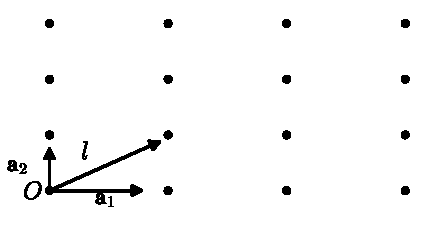
\includegraphics[width=0.72\textwidth]{fig_1.pdf}
\caption*{图 1\quad （原书此图无图注。）}
\end{figure}
\begin{figure}[H]
\centering
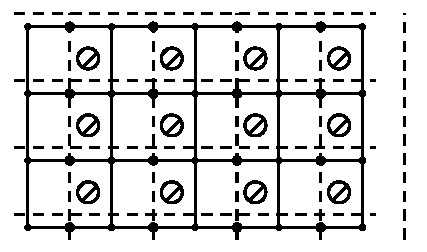
\includegraphics[width=0.72\textwidth]{fig_2.pdf}
\caption*{图 2\quad 可供选择的晶胞。}
\end{figure}
图 2 中看到的那样。或许不那么显而易见的是，晶胞的形状还可以在一定程度上加以改变。例如，假设结构中某一点具有中心对称性（因而在所有等价点处也都是如此）。这一点便很适合选作晶胞的中心，晶胞自身也具有中心对称性。系统地做到这一点的办法，是构造一个 Wigner–Seitz 原胞（Wigner–Seitz cell），也就是从选定的中心向最近邻的等价格点，画出各平移矢量的垂直平分面。全部平分面之内的体积显然是一个晶胞——它就是其中各点离选定中心比离任何其他格点都近的那个区域。

晶胞可以含有一个或多个原子。自然，如果只含一个原子，我们就把它置于格点中心，并说我们有一个 Bravais 格子（Bravais lattice）。如果每个晶胞含几个原子，那么我们就有了一个带基元的格子（lattice with a basis）。在后面的大部分内容中，我们将不加特别声明地假定结构是 Bravais 格子。这只是为简单起见；实际上只有少数几种单质固体——例如碱金属——才具有这种结构。

晶体学（crystallography）这门科学，关注的是对所有可能类型的晶体结构进行清点和分类，并确定实际晶体的实际结构。

\begin{figure}[H]
\centering
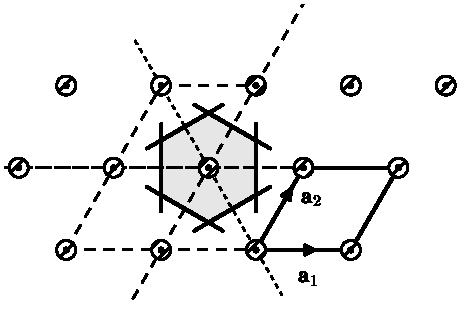
\includegraphics[width=0.72\textwidth]{fig_3.pdf}
\caption*{图 3\quad Wigner–Seitz 原胞。}
\end{figure}

结构按其对称性质分类，例如绕轴旋转的不变性、对平面反射的不变性等等。这些对称性常常对简化理论计算十分重要，并且在讨论定义固体宏观性质所需要的参数数目时，可以发挥很大的威力。然而，要充分利用这套理论，需要群论（group theory）这门数学，它会使我们偏离正题太远。如果我们主要局限于非常简单的固体，那么大多数对称性质无须正式的代数分析，单凭观察就能发现。无论如何，关于晶体学、以及关于群论及其在固体理论中的应用，都有许多优秀的著作。

在这些书中，各类 Bravais 格子等等都有详细的铺陈。我们在这里只考虑一个例子，它体现了本学科的许多原理，而且作为一种某些元素实际上采取的结构，也极为重要。这就是体心立方（body-centred cubic，B.C.C.）结构，如图 4 所示。

\begin{figure}[H]
\centering
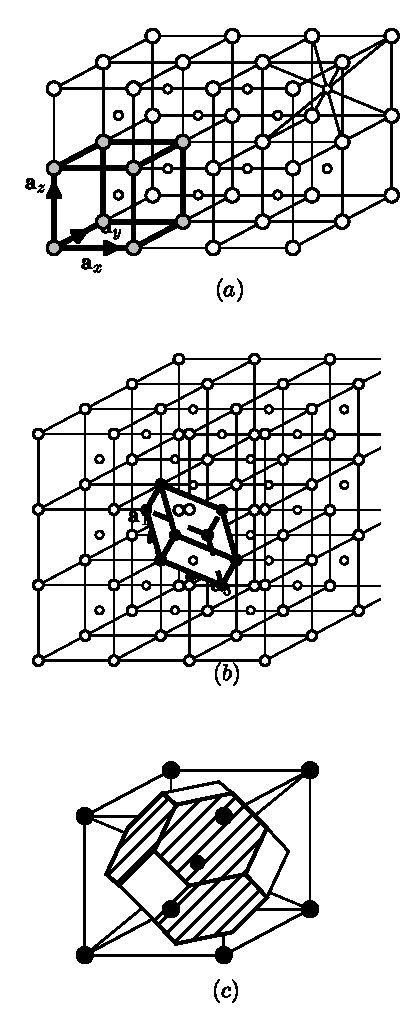
\includegraphics[width=0.6\textwidth]{fig_4.pdf}
\caption*{图 4\quad 体心立方格子。(a)立方晶胞。(b)Bravais 格子的生成矢。(c)Wigner–Seitz 原胞。}
\end{figure}

\begin{figure}[H]
\centering
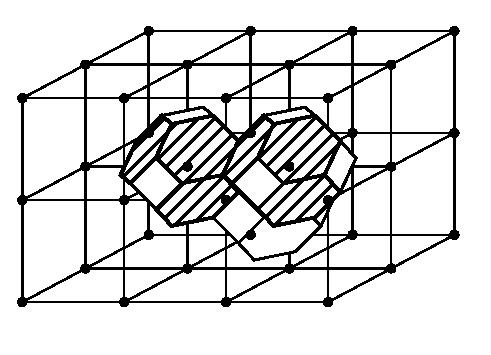
\includegraphics[width=0.72\textwidth]{fig_5.pdf}
\caption*{图 5\quad B.C.C. 格子 Wigner–Seitz 原胞的堆垛。}
\end{figure}

乍一看，这是一个每个立方晶胞含两个原子的格子，或者说是两个相互穿插的简立方亚格子，由
\begin{equation*}
\left.
\begin{aligned}
\boldsymbol{l} &= l_x\mathbf{a}_x + l_y\mathbf{a}_y + l_z\mathbf{a}_z, \\
\boldsymbol{l}' &= \left(l_x + \tfrac{1}{2}\right)\mathbf{a}_x + \left(l_y + \tfrac{1}{2}\right)\mathbf{a}_y + \left(l_z + \tfrac{1}{2}\right)\mathbf{a}_z,
\end{aligned}
\right\}
\tag{1.2}
\end{equation*}
定义，其中 $l_x$、$l_y$、$l_z$ 均为整数。但如果写下
\begin{equation*}
\left.
\begin{aligned}
\mathbf{a}_1 &= \tfrac{1}{2}\left(-\mathbf{a}_x + \mathbf{a}_y + \mathbf{a}_z\right), \\
\mathbf{a}_2 &= \tfrac{1}{2}\left(\mathbf{a}_x - \mathbf{a}_y + \mathbf{a}_z\right), \\
\mathbf{a}_3 &= \tfrac{1}{2}\left(\mathbf{a}_x + \mathbf{a}_y - \mathbf{a}_z\right),
\end{aligned}
\right\}
\tag{1.3}
\end{equation*}
我们便能由
\begin{equation*}
\boldsymbol{l} = l_1\mathbf{a}_1 + l_2\mathbf{a}_2 + l_3\mathbf{a}_3
\tag{1.4}
\end{equation*}
（$l_1$、$l_2$、$l_3$ 为整数）生成两个亚格子的全部格点。我们发现，落在立方体的中心还是顶角上，视 $(l_1+l_2+l_3)$ 为奇数还是偶数而定。

因此（图 4(b)），这其实是一个 Bravais 格子。我们可以不用立方晶胞，而改用 Wigner–Seitz 原胞（图 4(c)）；它的构造方法是，沿从中心到角点的对角线在半程处把立方体的各个角截去。这个图形显然具有与立方体相同的对称性——例如，原来的矢量 $\mathbf{a}_x$、$\mathbf{a}_y$、$\mathbf{a}_z$ 都是四重对称轴。它还（或许比原来的立方体更清楚地）表明，矢量 $\mathbf{a}_1$、$\mathbf{a}_2$、$\mathbf{a}_3$，即立方体的对角线，是三重旋转对称轴，因为它们穿过原胞的六边形面。设想一下这些多面体如何能堆砌成原来的格子（图 5），是一次很好的练习。

\section{周期函数}

要为一个晶体结构定义物理模型，我们需要给空间中的某个函数 $f(\mathbf{r})$ 赋值——局域电子密度、静电势等等，它们应能被辨认为原子的一种排列（例如图 6）。我们关于平移对称性的断言意味着，这必须是一个\emph{多重周期函数}（multiply periodic function）
\begin{equation*}
f(\mathbf{r}+\boldsymbol{l}) = f(\mathbf{r})
\tag{1.5}
\end{equation*}
对空间中所有的点 $\mathbf{r}$、对所有的格平移（lattice translations）都成立。

\begin{figure}[H]
\centering
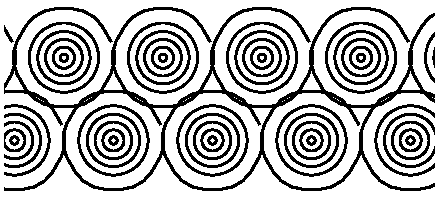
\includegraphics[width=0.72\textwidth]{fig_6.pdf}
\caption*{图 6\quad 多重周期函数。}
\end{figure}

\begin{figure}[H]
\centering
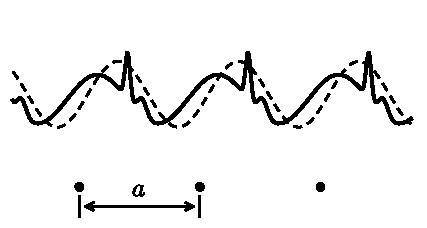
\includegraphics[width=0.72\textwidth]{fig_7.pdf}
\caption*{图 7\quad （原书此图无图注。）}
\end{figure}

在一维情形，我们对周期函数再熟悉不过了。例如，如图 7 那样，可以有
\begin{equation*}
f(x+l) = f(x),
\tag{1.6}
\end{equation*}
其中 $l$ 取 $l_1 a$ 的形式，$l_1$ 为整数，而 $a$ 是函数的周期。我们还知道，任何这类函数都可以表示成 Fourier 级数，
\begin{equation*}
f(x) = \sum_n A_n e^{2\pi i n x/a},
\tag{1.7}
\end{equation*}
其中 $n$ 是整数。让我们把它写成
\begin{equation*}
f(x) = \sum_g A_g e^{igx},
\tag{1.8}
\end{equation*}
其中的量 $g$ 属于倒格子长度（reciprocal lattice lengths）\footnote{在这个定义中把因子 $2\pi$ 包括进来是方便的；虽然在晶体学中惯例是把 $2\pi$ 明确地留在指数上。}的集合
\begin{equation*}
g_n = n\,\frac{2\pi}{a}.
\tag{1.9}
\end{equation*}

大家熟知，(1.8) 中的系数由
\begin{equation*}
A_g = \frac{1}{a}\int_{\text{cell}} f(x)\, e^{-igx}\, dx,
\tag{1.10}
\end{equation*}
定义；在这个例子里，积分范围譬如取 $0 < x \leqslant a$——它只需是晶格的一个晶胞。(1.8) 蕴含 (1.6) 这一初等证明，可以由如下条件导出：对任何 $g$ 值，
\begin{equation*}
e^{igl} = 1
\tag{1.11}
\end{equation*}
对所有平移 $l$ 成立。当 $g$ 取其一个允许值 $g_n$ 而 $l = l_1 a$ 时，这不过是说
\begin{equation*}
gl = n\,\frac{2\pi}{a}\, l_1 a = n l_1\, 2\pi = \text{integer} \times 2\pi
\tag{1.12}
\end{equation*}
罢了。(1.10) 的推导同样可以由这同一个关系得出。我们在这里不关心数学上病态的函数，尽可以放心地随意使用朴素的 Fourier 理论。

把这个定理推广到具有三条正交轴的结构相当容易。设这些轴为 $\mathbf{a}_x$、$\mathbf{a}_y$、$\mathbf{a}_z$，那么，只要
\begin{equation*}
f(\mathbf{r}+\boldsymbol{l}) \equiv f(\mathbf{r}+l_x\mathbf{a}_x+l_y\mathbf{a}_y+l_z\mathbf{a}_z) = f(\mathbf{r}),
\tag{1.13}
\end{equation*}
便有
\begin{equation*}
f(\mathbf{r}) = \sum_{g_x,g_y,g_z} A(g_x,g_y,g_z) \exp\left\{ i(g_x x + g_y y + g_z z)\right\},
\tag{1.14}
\end{equation*}
其中 $g_x$ 等等各自都是从集合 $2\pi n/a_x$ 等等中取的一个倒格子长度。证明可以这样做：先把 $f(\mathbf{r})$ 沿 $x$ 方向展开成 Fourier 级数，然后证明该级数的每个系数都是 $y$ 的周期函数，因而可以再展开成一个级数——对 $z$ 亦照此办理。

让我们把 (1.14) 改写成
\begin{equation*}
f(\mathbf{r}) = \sum_{\boldsymbol{g}} A_{\boldsymbol{g}} e^{i\boldsymbol{g}\cdot\mathbf{r}},
\tag{1.15}
\end{equation*}
其中 $\boldsymbol{g}$ 是分量为 $(g_x,g_y,g_z)$ 的矢量。这种矢量具有 (1.11) 所表达的性质，也就是说，对任何一个这样的矢量
\begin{align*}
\boldsymbol{g}\cdot\boldsymbol{l} &= \left(g_x l_x \mathbf{a}_x + g_y l_y \mathbf{a}_y + g_z l_z \mathbf{a}_z\right) \\
&= \frac{2\pi n_x}{a_x} l_x \mathbf{a}_x + \frac{2\pi n_y}{a_y} l_y \mathbf{a}_y + \frac{2\pi n_z}{a_z} l_z \mathbf{a}_z \\
&= 2\pi \times \text{integer},
\tag{1.16}
\end{align*}
无论 $\boldsymbol{l}$ 取什么值。于是，
\begin{equation*}
e^{i\boldsymbol{g}\cdot\boldsymbol{l}} = 1
\tag{1.17}
\end{equation*}
对一切格矢 $\boldsymbol{l}$、对一切倒格矢（reciprocal lattice vector）$\boldsymbol{g}$ 都成立。

显然，这个条件足以使级数 (1.15) 表示一个像 (1.5) 那样具有晶格周期性的函数：
\begin{align*}
f(\mathbf{r}+\boldsymbol{l}) &= \sum_{\boldsymbol{g}} A_{\boldsymbol{g}}\, e^{i\boldsymbol{g}\cdot(\mathbf{r}+\boldsymbol{l})} = \sum_{\boldsymbol{g}} A_{\boldsymbol{g}}\, e^{i\boldsymbol{g}\cdot\mathbf{r}}\, e^{i\boldsymbol{g}\cdot\boldsymbol{l}} \\
&= \sum_{\boldsymbol{g}} A_{\boldsymbol{g}}\, e^{i\boldsymbol{g}\cdot\mathbf{r}} = f(\mathbf{r}).
\tag{1.18}
\end{align*}
人们不难设计出一个证明，说明它也是必要条件，也就是说，级数 (1.15) 中只能含有 $g$ 值满足条件 (1.17) 的那些项。

剩下的只是为非正交格子构造倒格矢。这很容易做到：取基矢的倒格子三矢组（reciprocal triad），即
\begin{equation*}
\mathbf{b}_1 = \frac{\mathbf{a}_2\wedge\mathbf{a}_3}{\mathbf{a}_1\cdot\mathbf{a}_2\wedge\mathbf{a}_3}, \qquad
\mathbf{b}_2 = \frac{\mathbf{a}_3\wedge\mathbf{a}_1}{\mathbf{a}_1\cdot\mathbf{a}_2\wedge\mathbf{a}_3}, \qquad
\mathbf{b}_3 = \frac{\mathbf{a}_1\wedge\mathbf{a}_2}{\mathbf{a}_1\cdot\mathbf{a}_2\wedge\mathbf{a}_3},
\tag{1.19}
\end{equation*}
并写出
\begin{align*}
\boldsymbol{g} &= g_1\mathbf{b}_1 + g_2\mathbf{b}_2 + g_3\mathbf{b}_3 \\
&= 2\pi n_1\mathbf{b}_1 + 2\pi n_2\mathbf{b}_2 + 2\pi n_3\mathbf{b}_3,
\tag{1.20}
\end{align*}
其中 $n_1$ 等等为整数。

由初等矢量分析即可验证：$\mathbf{b}_1\cdot\mathbf{a}_1 = 1$ 等等，以及 $\mathbf{b}_1\cdot\mathbf{a}_2 = 0$ 等等；于是
\begin{align*}
\boldsymbol{g}\cdot\boldsymbol{l} &= \left(g_1\mathbf{b}_1 + g_2\mathbf{b}_2 + g_3\mathbf{b}_3\right)\cdot\left(l_1\mathbf{a}_1 + l_2\mathbf{a}_2 + l_3\mathbf{a}_3\right) \\
&= g_1 l_1 + g_2 l_2 + g_3 l_3 \\
&= 2\pi \times \text{integer}.
\tag{1.21}
\end{align*}
因此，集合 (1.20) 中的每一个矢量都满足条件 (1.17)。

我们还可以把公式 (1.10) 加以推广，用来求级数 (1.15) 中的每个系数。它必须是一个体积分，我们把它写作
\begin{equation*}
A_{\boldsymbol{g}} = \frac{1}{v_{\text{cell}}} \int_{\text{cell}} f(\mathbf{r})\, e^{-i\boldsymbol{g}\cdot\mathbf{r}}\,\mathrm{d}\mathbf{r}.
\tag{1.22}
\end{equation*}

%（以下为 §1.2 的收尾段落，印于书页 9 顶部，接式 (1.22) 之后）
证明只需把整个级数乘以 $\exp(-i\boldsymbol{g}\cdot\mathbf{r})$，然后积分。若 $\boldsymbol{g}$ 具有 (1.20) 的形式，则 $\exp(i\boldsymbol{g}\cdot\mathbf{r})$ 在一个晶胞上的积分显然为零，除非 $\boldsymbol{g}=0$。

\section{倒格子的性质}

由 (1.20) 定义的矢量，即
\begin{equation*}
\boldsymbol{g} = n_1\cdot 2\pi\mathbf{b}_1 + n_2\cdot 2\pi\mathbf{b}_2 + n_3\cdot 2\pi\mathbf{b}_3,
\tag{1.23}
\end{equation*}
生成一个点阵，其晶胞由矢量 $2\pi\mathbf{b}_1$、$2\pi\mathbf{b}_2$、$2\pi\mathbf{b}_3$ 张成。这就是我们原来正格子（direct lattice）的倒格子（reciprocal lattice）。它是一个不变的几何客体，其性质是固体理论的基础。它的几个初等几何性质很容易推导。

(i) \emph{倒格子的每一个矢量都垂直于正格子的一族点阵面（lattice planes）。}

任取一个倒格矢 $\boldsymbol{g}$ 和一个格矢 $\boldsymbol{l}$，考虑关系式 (1.21)：
\begin{align*}
\boldsymbol{g}\cdot\boldsymbol{l} &= 2\pi(n_1 l_1 + n_2 l_2 + n_3 l_3) \\
&= 2\pi N,
\tag{1.24}
\end{align*}
其中 $N$ 是整数。这告诉我们，矢量 $\boldsymbol{l}$ 在 $\boldsymbol{g}$ 方向上的投影长度为
\begin{equation*}
d = \frac{2\pi N}{|\boldsymbol{g}|}.
\tag{1.25}
\end{equation*}
但是，具有这一性质的格点有无穷多个。例如，设 $\boldsymbol{l}'$ 是由整数
\begin{equation*}
l'_1 = l_1 - mn_3, \qquad l'_2 = l_2 - mn_3, \qquad l'_3 = l_3 + m(n_1+n_2),
\tag{1.26}
\end{equation*}
所代表的格点，其中 $m$ 是整数（译注：原书第三式误印作 $l_1+m(n_1+n_2)$，按上下文应为 $l_3$）。显然
\begin{equation*}
\boldsymbol{g}\cdot\boldsymbol{l}' = \boldsymbol{g}\cdot\boldsymbol{l} = 2\pi N.
\tag{1.27}
\end{equation*}
于是 $\boldsymbol{l}'$ 在 $\boldsymbol{g}$ 上的投影与 $\boldsymbol{l}$ 相同，因而必定也位于与 $\boldsymbol{g}$ 垂直、距原点为 $d$ 的平面上。这样，若这个平面上有一个格点，其上就有无穷多个格点；我们便构造出了一个\emph{点阵面}。正格子与倒格子之间的这种关系，当然是三维几何中人所共知的点与平面对偶性的一个特例。

(ii) \emph{若 $\boldsymbol{g}$ 的分量没有公因子，则 $|\boldsymbol{g}|$ 与垂直于 $\boldsymbol{g}$ 的点阵面的间距成反比。}

这由式 (1.25) 可得（见图 8）。若 $(n_1, n_2, n_3)$ 没有公因子，则总能找到一个格矢 $\boldsymbol{l}''$，其分量满足
\begin{equation*}
\boldsymbol{g}\cdot\boldsymbol{l}'' = 2\pi(N+1).
\tag{1.28}
\end{equation*}
这意味着，包含 $\boldsymbol{l}''$ 的点阵面位于距原点
\begin{equation*}
d'' = \frac{2\pi(N+1)}{|\boldsymbol{g}|}
\tag{1.29}
\end{equation*}
处——亦即它与包含 $\boldsymbol{l}$ 的点阵面相距 $2\pi/|\boldsymbol{g}|$。

\begin{figure}[H]
\centering
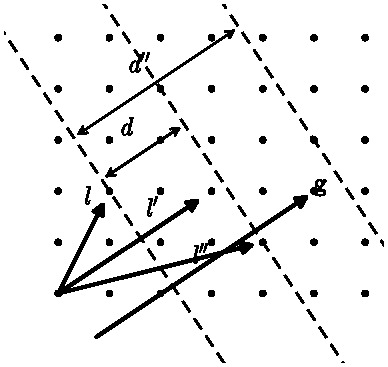
\includegraphics[width=0.72\textwidth]{fig_8.pdf}
\caption*{图 8\quad （原书此图无图注。）}
\end{figure}

从这两个初等几何结果可以看出，表征点阵诸平面最简单的方式就是用它们的法线，把它们表示为倒格矢。正格子中最显著的平面，是格点最密集的那些平面。由于格点在空间中的密度是常数，最显著的平面必定是相隔最远的那些平面，即具有最小倒格矢的那些平面。

用相应的倒格矢来标示点阵面，等价于经典结晶学中所用的米勒指数（Miller indices）。设有一个点阵面，法线为 $\boldsymbol{g}$，其上所有的点 $\boldsymbol{l}$ 都满足 (1.24)。取 $l_2 = l_3 = 0$ 的点，则得 $l_1 = N/n_1$，于是这个平面沿 $\mathbf{a}_1$ 轴的截距长度为
\begin{equation*}
d_1 = \left(\frac{N}{n_1}\right) a_1.
\tag{1.30}
\end{equation*}
类似地，这个平面与 $\mathbf{a}_2$ 轴相交于距原点
\begin{equation*}
d_2 = \left(\frac{N}{n_2}\right) a_2
\tag{1.31}
\end{equation*}
处。该平面沿各轴的截距，以相应基矢的长度为单位来量度，与整数 $n_1$、$n_2$、$n_3$ 成反比。除去公因子之后，这些整数就是这个点阵面的米勒指数，写成 $(n_1, n_2, n_3)$ 的形式。

显然，格点密集的面——即米勒指数小的面——最容易在天然晶体中出现，无论是在生长时还是解理之后。研究这类晶面的几何曾是经典结晶学的精髓，而其
\begin{figure}[H]
\centering
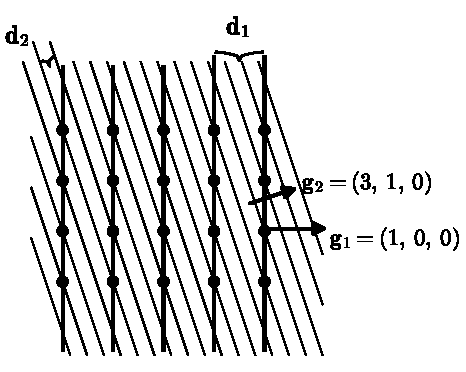
\includegraphics[width=0.72\textwidth]{fig_9.pdf}
\caption*{图 9\quad 具有大米勒指数的晶面，其间距比主对称面的间距更小。}
\end{figure}
关键性的发现是：可以找到单独一组矢量 $\mathbf{a}_1$、$\mathbf{a}_2$、$\mathbf{a}_3$，使得宏观晶体上所有观察到的晶面都能用小的米勒指数来表示。

应当提到两种记号约定。符号 $(1\bar{1}\bar{1})$ 代表 $(1,-1,-1)$ 这组平面；为简洁起见，把负号写在数字上方。带花括号的符号 $\{110\}$ 代表在对称性上与 $(110)$ 等价的各组不同的平面。因此，对立方结构而言，它可以包括 $(101)$、$(011)$、$(\bar{1}\bar{1}0)$、$(1\bar{1}0)$，等等。

(iii) \emph{倒格子晶胞的体积与正格子晶胞的体积成反比。}

这用初等矢量分析即可得出。倒格子晶胞由 $2\pi\mathbf{b}_1$、$2\pi\mathbf{b}_2$、$2\pi\mathbf{b}_3$ 张成。利用 (1.19)，其体积为
\begin{align*}
(2\pi)^3(\mathbf{b}_1\cdot\mathbf{b}_2\wedge\mathbf{b}_3)
&= (2\pi)^3
\frac{(\mathbf{a}_2\wedge\mathbf{a}_3)\cdot\{(\mathbf{a}_3\wedge\mathbf{a}_1)\wedge(\mathbf{a}_1\wedge\mathbf{a}_2)\}}
{(\mathbf{a}_1\cdot\mathbf{a}_2\wedge\mathbf{a}_3)^3} \\
&= (2\pi)^3
\frac{(\mathbf{a}_2\wedge\mathbf{a}_3)\cdot[\{\mathbf{a}_3\cdot(\mathbf{a}_1\wedge\mathbf{a}_2)\}\mathbf{a}_1 - \{\mathbf{a}_1\cdot(\mathbf{a}_1\wedge\mathbf{a}_2)\}\mathbf{a}_3]}
{(\mathbf{a}_1\cdot\mathbf{a}_2\wedge\mathbf{a}_3)^3} \\
&= \frac{(2\pi)^3}{(\mathbf{a}_1\cdot\mathbf{a}_2\wedge\mathbf{a}_3)} \\
&= \frac{8\pi^3}{v_c},
\tag{1.32}
\end{align*}
其中 $v_c$ 是由 $\mathbf{a}_1$、$\mathbf{a}_2$、$\mathbf{a}_3$ 张成的晶胞的体积。

这里出现因子 $8\pi^3$，是由于我们对倒格子的定义方式。更常见的约定是写成
\begin{equation*}
e^{i\boldsymbol{g}\cdot\boldsymbol{l}} \equiv \exp(2\pi i\,\mathbf{K}_g\cdot\mathbf{R}_l),
\tag{1.33}
\end{equation*}
其中 $\mathbf{R}_l$ 是格矢，而矢量 $\mathbf{K}_g$ 定义为晶胞体积为 $1/v_c$ 的另一个倒格子的矢量。这种记法的缺点是因子 $2\pi$ 总是在指数中冒出来；它也同自由电子波函数的惯用符号
\begin{equation*}
\psi = e^{i\mathbf{k}\cdot\mathbf{r}}
\tag{1.34}
\end{equation*}
不相协调。

(iv) \emph{正格子正是它自己的倒格子的倒格子。}

这已隐含在名称之中，也可以通过构造例如矢量 $(\mathbf{b}_1\wedge\mathbf{b}_2)/(\mathbf{b}_1\cdot\mathbf{b}_2\wedge\mathbf{b}_3)$ 并证明它与 $\mathbf{a}_3$ 全同来验证。考察 (1.32) 的推导过程也能看出这一点。

(v) \emph{倒格子的晶胞不必是平行六面体。}事实上，我们几乎总是在同倒格子的 Wigner--Seitz 胞（Wigner--Seitz cell）打交道。它叫做布里渊区（Brillouin zone）。

作为倒格子诸性质的一个例子，考虑一种重要且常见的结构——面心立方（face-centred cubic）格子（f.c.c. 结构）。它由四个相互穿插的简单立方格子搭成；随便看其中哪一个，都会看到它的晶胞每个面的中心各有一个原子，同时立方体的角上也分布着格点（图 10(a)）。

乍一看，这像一个带基元的格子：由 $(\mathbf{a}_x,\mathbf{a}_y,\mathbf{a}_z)$ 生成的立方晶胞里有四个原子。

但是，如果改取立方体各个面的半对角线
\begin{equation*}
\left.
\begin{aligned}
\mathbf{a}_1 &= (0, \tfrac{1}{2}a, \tfrac{1}{2}a), \qquad
\mathbf{a}_2 = (\tfrac{1}{2}a, 0, \tfrac{1}{2}a), \\
\mathbf{a}_3 &= (\tfrac{1}{2}a, \tfrac{1}{2}a, 0),
\end{aligned}
\right\}
\tag{1.35}
\end{equation*}
\begin{figure}[H]
\centering
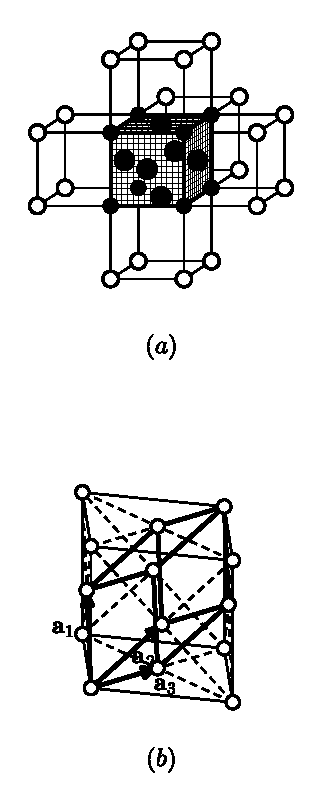
\includegraphics[width=0.58\textwidth]{fig_10.pdf}
\caption*{图 10\quad 面心立方格子。(a) 四个相互穿插的子晶格。(b) 作为 Bravais 格子。}
\end{figure}

那么用这些矢量的倍数的组合就能到达任何一个格点（图 10(b)）。因此，f.c.c. 格子确实是一个 Bravais 格子，$\mathbf{a}_1$、$\mathbf{a}_2$、$\mathbf{a}_3$ 就是它的生成矢。

现在我们本可以用代数方法构造出倒格子来，但利用上面指出的几何性质更为容易。例如，显然存在垂直于立方体棱边的重要点阵面。相对沿 $\mathbf{a}_x$、$\mathbf{a}_y$、$\mathbf{a}_z$ 方向的通常笛卡儿轴而言，这些面的米勒指数必为 (100)、(010)、(001) 等，即它们构成 $\{100\}$ 组。还可以看出，这些面彼此相距 $\tfrac{1}{2}a$。于是，它们对应于长度为
\begin{equation*}
|\boldsymbol{g}| = 2\pi/\tfrac{1}{2}a
\end{equation*}
沿倒格子空间中直角笛卡儿轴方向的倒格矢。我们的倒格子必须包含由这些矢量生成的整个简单立方格子。

还有一种重要的点阵面垂直于立方晶胞的对角线。这种面在三条轴上的截距相等，故其指数必属 $\{111\}$ 组。这些面
\begin{figure}[H]
\centering
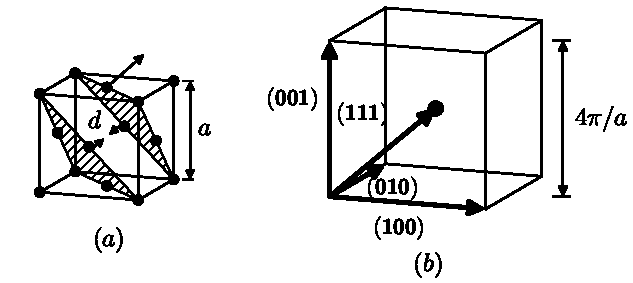
\includegraphics[width=0.72\textwidth]{fig_11.pdf}
\caption*{图 11\quad (a) f.c.c. 格子的 {111} 面。(b) 相应的倒格子晶胞。}
\end{figure}
彼此相隔的距离等于立方体整条对角线的三分之一，即 $a/\sqrt{3}$。因此，相应的倒格矢有三个相等的分量，总长为 $2\pi\sqrt{3}/a$；它必是
\begin{equation*}
\boldsymbol{g}' = \frac{2\pi}{a}(1, 1, 1).
\tag{1.36}
\end{equation*}
在倒格子空间中，它显然沿立方晶胞对角线的方向——但长度只有对角线的一半。于是，它生成简单立方格子的各个体心。

其余的点阵面现在都可以如法研究——例如 $\{110\}$ 组面，它们垂直于基本立方体各面的对角线——不过与它们相应的倒格矢全都已经包含在由 $\{100\}$ 面和 $\{111\}$ 面生成的那些点之中。因此，f.c.c. 格子的倒格子是 b.c.c.（当然，反之亦然）。

f.c.c.格子的布里渊区就是这个倒格子的Wigner–Seitz原胞。这个图形我们已经在图 4(c)中见过——一个兼有正方形面与六边形面的多面体。正方形面的中心对应于正格子诸立方晶面法线的方向；六边形面的中心则是诸对角面法线的方向。

还有一点颇有意思：f.c.c.结构是一种“密堆积”（close-packed）结构。依次叠合一层层(111)面就可以把它构造出来，每一层都是一个六边形网络，就像由刚性球排成的那样。这也是金属常常采取这种结构的原因之一：金属的内聚并不依赖于强方向性的键，而在很大程度上是一种体积效应。

\section{Bloch 定理}

我们已经学会了如何表示具有晶格周期性的函数。但对于一种物理理论来说这些还不够；我们还需要考虑结构的各种激发，它们会破坏严格的平移对称性。这类激发有若干种，其中最重要的是格波（lattice waves），即原子绕其平衡位置的振动；以及电子态（electron states），即电子在静态晶格的场中的运动。在第10章我们还将考虑自旋波（spin waves），即定域在晶体各原子上的那些自旋的激发。

所有这些激发都以一个动力学方程——或一个Schrödinger方程，或一个自旋交换哈密顿量——为特征，它们\emph{在晶格平移下不变}。于是，若 $\mathcal{V}(\mathbf{r})$ 是位于 $\mathbf{r}$ 处的电子所感受到的势，则对一切 $\mathbf{l}$ 都有 $\mathcal{V}(\mathbf{r}+\mathbf{l})=\mathcal{V}(\mathbf{r})$。电子的波函数 $\psi(\mathbf{r})$ 必须满足Schrödinger方程
\begin{equation*}
\left(-\frac{\hbar^{2}}{2m}\nabla^{2}+\mathcal{V}(\mathbf{r})-\mathcal{E}\right)\psi=0,
\tag{1.37}
\end{equation*}
在把作用于 $\psi$ 的算符中的 $\mathbf{r}$ 换成 $\mathbf{r}+\mathbf{l}$ 之后，这个方程保持不变。

在格波和自旋波的情形，形式体系要更复杂一些，但原理相同。设
\begin{equation*}
(u_1,\,u_2,\,\dots,\,u_{\mathbf{n}},\,\dots)
\end{equation*}
是位于 $1,2,\dots,\mathbf{n},\dots$ 各格点上的原子的位移（或自旋位移，或自旋偏离算符，或随便什么东西）。运动方程（或哈密顿量）将把这些变量（或算符）包含在内，其方式是：如果我们作一个晶格平移 $\mathbf{l}$——也就是说，把公式里原先出现 $u_{\mathbf{n}}$ 的地方统统换成 $u_{\mathbf{n}+\mathbf{l}}$——我们将看不出任何差别。换言之，晶格的所有晶胞都等价而且不可分辨。这颇像所谓“宇宙学原理”（cosmological principle）：无论我们从哪一点观察，宇宙看起来本质上都是一样的。

为了把这个性质形式化，我们采用如下记号。令 $\mathcal{H}(\mathbf{0})$ 和 $|0\rangle$ 表示晶格平移之前的哈密顿算符和波函数；令 $\mathcal{H}(\mathbf{l})$ 和 $|\mathbf{l}\rangle$ 表示平移 $\mathbf{l}$ 之后的同样一些数学对象。于是，对电子而言 $|0\rangle\equiv\psi(\mathbf{r})$，$|\mathbf{l}\rangle\equiv\psi(\mathbf{r}+\mathbf{l})$。对格波而言，若 $|0\rangle$ 表示位于 $\mathbf{n}$ 处的原子正经历某一特定运动的态，则 $|\mathbf{l}\rangle$ 就表示位于 $(\mathbf{n}+\mathbf{l})$ 处的原子正作同一运动的态。

平移不变性的表述便是
\begin{equation*}
\mathcal{H}(\mathbf{l})=\mathcal{H}(\mathbf{0}).
\tag{1.38}
\end{equation*}
现在，本征态必须满足如下形式的方程\footnote{在格波的经典运动方程的情形，频率 $\omega$ 的平方扮演能量的角色，而“哈密顿量”则是在我们假定所处理的是对平衡的小偏离时导出的那组联立线性微分方程的矩阵。参看 §2.1。}
\begin{equation*}
\mathcal{H}(\mathbf{0})\,|0\rangle=\mathcal{E}\,|0\rangle.
\tag{1.39}
\end{equation*}
这个方程与
\begin{equation*}
\mathcal{H}(\mathbf{l})\,|\mathbf{l}\rangle=\mathcal{E}\,|\mathbf{l}\rangle,
\tag{1.40}
\end{equation*}
完全相同，后者只不过是把算符与态函数中的所有变量作一次形式上的重新标记而已。但由式 (1.38)，这意味着
\begin{equation*}
\mathcal{H}(\mathbf{0})\,|\mathbf{l}\rangle=\mathcal{E}\,|\mathbf{l}\rangle,
\tag{1.41}
\end{equation*}
也就是说，态函数 $|\mathbf{l}\rangle$ 也是 $|0\rangle$ 所满足的那个方程的解。由于 $|\mathbf{l}\rangle$ 未必与 $|0\rangle$ 恒同，看上去我们似乎只要把碰巧找到的任何一个解加以平移，就能生成运动方程的数不清的解。当然，所有这些解在能量上都是简并的。

这显然是荒谬的；新解必定都以某种方式与我们原来的解等价。有两种情形需要考虑：

(i) 设 $|0\rangle$ 确实是\emph{非简并}的（这种情况实际上绝不会发生，因为一切晶格除平移不变性之外还具有镜面对称性）。那么唯一的可能是：每个新态 $|\mathbf{l}\rangle$ 都是 $|0\rangle$ 的某个倍数，从而在物理上与它不可分辨。必定存在某个数 $\lambda_1$，使得
\begin{equation*}
|\mathbf{a}_1\rangle=\lambda_1|0\rangle
\tag{1.42}
\end{equation*}
这是沿 $\mathbf{a}_1$ 方向走一步的结果。归一化要求
\begin{equation*}
|\lambda_1|^{2}=1,
\tag{1.43}
\end{equation*}
于是可以取
\begin{equation*}
\lambda_1=e^{ik_1},
\tag{1.44}
\end{equation*}
其中 $k_1$ 为实数。类似地，对其余两个基本方向上的单位平移，可以取
\begin{equation*}
|\mathbf{a}_2\rangle=e^{ik_2}|0\rangle;\qquad|\mathbf{a}_3\rangle=e^{ik_3}|0\rangle,
\tag{1.45}
\end{equation*}
于是一般平移必须导致如下关系
\begin{align*}
|\mathbf{l}\rangle&\equiv|l_1\mathbf{a}_1+l_2\mathbf{a}_2+l_3\mathbf{a}_3\rangle\notag\\
&=e^{ik_1}|(l_1-1)\mathbf{a}_1+l_2\mathbf{a}_2+l_3\mathbf{a}_3\rangle\notag\\
&=e^{ik_1 l_1}|0+l_2\mathbf{a}_2+l_3\mathbf{a}_3\rangle\notag\\
&=e^{i(k_1 l_1+k_2 l_2+k_3 l_3)}|0\rangle
\tag{1.46}
\end{align*}
这里我们沿 $\mathbf{a}_1$ 方向走 $l_1$ 步、沿 $\mathbf{a}_2$ 方向走 $l_2$ 步，如此等等，每走一步都乘上相应的因子。

我们按如下形式定义一个矢量 $\mathbf{k}$：
\begin{equation*}
\mathbf{k}=k_1\mathbf{b}_1+k_2\mathbf{b}_2+k_3\mathbf{b}_3,
\tag{1.47}
\end{equation*}
其中 $\mathbf{b}_1,\mathbf{b}_2,\mathbf{b}_3$ 是 $\mathbf{a}_1,\mathbf{a}_2,\mathbf{a}_3$ 的倒三基矢（reciprocal triad），如式 (1.19) 中那样。关系式 (1.46) 便成为
\begin{equation*}
|\mathbf{l}\rangle=e^{i\mathbf{k}\cdot\mathbf{l}}|0\rangle,
\tag{1.48}
\end{equation*}
这正是我们想要证明的结果：

\emph{对于任何一个满足Schrödinger方程（或其经典或量子的对应形式）的波函数/态函数，都存在一个矢量 $\mathbf{k}$，使得平移一个格矢 $\mathbf{l}$ 等价于乘上相位因子 $\exp(i\mathbf{k}\cdot\mathbf{l})$。}

每个不同的态函数可以有不同的波矢（wave-vector）$\mathbf{k}$，但每一个都必须满足这个条件。晶格具有平移不变性这个强的初始前提，对元激发的形式强加了一条强的限制条件。

但我们还需要在更一般的情形下给出证明。

(ii) 设 $|0\rangle$ 是简并的。为简单起见，设它是二重简并的，于是肯定存在两个能量相同而又彼此不同的态 $|0\rangle_1$ 和 $|0\rangle_2$。那么，晶格平移 $\mathbf{a}_1$ 至多能产生这两个态本身的线性组合。于是
\begin{equation*}
\left.\begin{aligned}
|\mathbf{a}_1\rangle_1&=\mathsf{T}_1^{11}\,|0\rangle_1+\mathsf{T}_1^{12}\,|0\rangle_2,\\
|\mathbf{a}_1\rangle_2&=\mathsf{T}_1^{21}\,|0\rangle_1+\mathsf{T}_1^{22}\,|0\rangle_2,
\end{aligned}\right\}
\tag{1.49}
\end{equation*}
诸数 $\mathsf{T}_1^{11}$ 等之所以这样书写，是因为它们是矩阵 $\mathsf{T}_1$ 的元素；为了保持归一化，$\mathsf{T}_1$ 必须是幺正矩阵（unitary matrix）。为简洁起见，把这对方程写成
\begin{equation*}
\left(\,|\mathbf{a}_1\rangle\right)=\mathsf{T}_1\left(\,|0\rangle\right).
\tag{1.50}
\end{equation*}
但 $|0\rangle_1$ 和 $|0\rangle_2$ 既然是简并的，就不是唯一定义的。我们原本可以从任何另外两个态出发，只要它们是这两个态的线性组合。例如，我们也许可以从
\begin{equation*}
\left.\begin{aligned}
|0\rangle_1&=\mathsf{S}^{11}\,|0\rangle_1+\mathsf{S}^{12}\,|0\rangle_2,\\
|0\rangle_2&=\mathsf{S}^{21}\,|0\rangle_1+\mathsf{S}^{22}\,|0\rangle_2,
\end{aligned}\right\}
\tag{1.51}
\end{equation*}
出发，其中诸数 $\mathsf{S}^{11}$ 等是另一个（任意的）幺正矩阵 $\mathsf{S}$ 的元素。

现在我们这样选取 $\mathsf{S}$，使矩阵 $\mathsf{S}\mathsf{T}_1\mathsf{S}^{-1}$ 成为对角矩阵。按标准的代数理论，这总是做得到的。例如，设它约化为如下形式
\begin{equation*}
\mathsf{S}\mathsf{T}_1\mathsf{S}^{-1}=
\begin{pmatrix}
e^{ik_1} & 0\\
0 & e^{ik_1'}
\end{pmatrix}.
\tag{1.52}
\end{equation*}
很容易验证，态 $|0\rangle_1$ 和 $|0\rangle_2$ 现在在平移之下的变换方式，恰好就像它们是非简并的一样，即如式 (1.42–1.45) 中那样：
\begin{equation*}
|\mathbf{a}_1\rangle_1=e^{ik_1}|0\rangle_1,\qquad|\mathbf{a}_1\rangle_2=e^{ik_1'}|0\rangle_2.
\tag{1.53}
\end{equation*}
态 $|0\rangle_1$ 有一个波矢，其在 $\mathbf{a}_1$ 方向上的分量为 $k_1$；态 $|0\rangle_2$ 对同一平移方向则有一个分量为 $k_1'$（一般说来与之不同）的波矢。

但是其他方向的平移又如何呢？考虑 $\mathbf{a}_2$。对初始态 $|0\rangle_1$ 和 $|0\rangle_2$，将有另一个矩阵 $\mathsf{T}_2$ 确定这一平移的结果，即像式 (1.49) 和 (1.50) 中那样符号式地写成
\begin{equation*}
\left(\,|\mathbf{a}_2\rangle\right)=\mathsf{T}_2\left(\,|0\rangle\right).
\tag{1.54}
\end{equation*}
现在我们也可以把这个矩阵 $\mathsf{T}_2$ 化成对角形式，正如式 (1.52) 中那样，只要选好一组适当的起始函数。乍一看，这似乎与我们用来使 $\mathsf{T}_1$ 对角化的那组函数不相容。但请考虑如下两种可供选择的约化：
\begin{equation*}
\left(\,|\mathbf{a}_1+\mathbf{a}_2\rangle\right)=
\left\{\begin{aligned}
\mathsf{T}_2(\,|\mathbf{a}_1\rangle)&=\mathsf{T}_2\mathsf{T}_1(\,|0\rangle),\\
\mathsf{T}_1(\,|\mathbf{a}_2\rangle)&=\mathsf{T}_1\mathsf{T}_2(\,|0\rangle).
\end{aligned}\right\}
\tag{1.55}
\end{equation*}
矩阵 $\mathsf{T}_1$ 和 $\mathsf{T}_2$ 由此彼此对易。矩阵代数中有一条定理告诉我们：这时存在一个幺正矩阵 $\mathsf{S}$，使得 $\mathsf{T}_1$ 和 $\mathsf{T}_2$ \emph{二者}都能\emph{同时}约化为对角形式。于是，态 $|0\rangle_1$ 和 $|0\rangle_2$ 不会被平移 $\mathbf{a}_2$ 混合，而只是被乘上相位因子
\begin{equation*}
|\mathbf{a}_2\rangle_1=e^{ik_2}|0\rangle_1,\qquad|\mathbf{a}_2\rangle_2=e^{ik_2'}|0\rangle_2.
\tag{1.56}
\end{equation*}
对平移 $\mathbf{a}_3$ 也有类似的结果，于是我们基本上回到了与式 (1.45) 实质相同的情形：对 $|0\rangle_1$ 和 $|0\rangle_2$ 中的每一个都存在一个波矢，使得
\begin{equation*}
|\mathbf{l}\rangle=e^{i\mathbf{k}\cdot\mathbf{l}}|0\rangle.
\tag{1.57}
\end{equation*}
把这一论证推广到两个以上能量简并的态，显然是轻而易举的。

这样，定理便在一般情形下得证，其含义是：波函数的任何一个简并解都可以表示成一些同能量解的线性组合，其中每一个都必须满足这类条件，尽管并非全都取同一个 $\mathbf{k}$ 值。

这就是\emph{Bloch定理}。其实，还存在一个一般的群论证明，它是下述定理的一条推论：“在复数域中，Abel群的任何表示都可以约化为若干一维表示之和”。晶体的平移群是Abel群——也就是说，群的所有元素彼此对易。这来自一个明显的事实：比如平移 $(\mathbf{a}_1+\mathbf{a}_2)$ 与 $(\mathbf{a}_2+\mathbf{a}_1)$ 是同一回事——我们可以沿许多不同的路径到达一个格点，但结果完全一样。矩阵 $\mathsf{T}_1$、$\mathsf{T}_2$ 等等正是这些平移的表示，因而可以约化为对角形式。

\section{约化到一个布里渊区}

Bloch定理的普遍性如此之强，以致在这个阶段我们很难把握它。对电子波而言，它意味着我们可以用波矢 $\mathbf{k}$ 来标记每一个波函数，并写成
\begin{equation*}
\psi_{\mathbf{k}}(\mathbf{r}+\mathbf{l})=e^{i\mathbf{k}\cdot\mathbf{l}}\psi_{\mathbf{k}}(\mathbf{r}).
\tag{1.58}
\end{equation*}
我们注意到，普通的自由电子波满足这个条件：
\begin{equation*}
\psi_{\mathbf{k}}(\mathbf{r})=e^{i\mathbf{k}\cdot\mathbf{r}}.
\tag{1.59}
\end{equation*}
这是意料之中的，因为我们处理的仍然是在周期势中Schrödinger方程的解；只不过这个势碰巧处处为零。空晶格检验（empty-lattice test）在固体理论中往往非常有用。

有时为了方便，人们试图让具有给定 $\mathbf{k}$ 值的电子波函数尽可能看起来像自由电子波。我们令
\begin{equation*}
\psi_{\mathbf{k}}(\mathbf{r})=e^{i\mathbf{k}\cdot\mathbf{r}}u_{\mathbf{k}}(\mathbf{r})
\tag{1.60}
\end{equation*}
并指望 $u_{\mathbf{k}}$ 将近乎恒定。事实上，由式 (1.58) 立刻可以证明，函数 $u_{\mathbf{k}}(\mathbf{r})$ 必须是周期的，即
\begin{equation*}
u_{\mathbf{k}}(\mathbf{r}+\mathbf{l})=u_{\mathbf{k}}(\mathbf{r}).
\tag{1.61}
\end{equation*}
Bloch定理有时就表述成这种形式。

定理中出现的因子 $\exp(i\mathbf{k}\cdot\mathbf{l})$，与我们研究周期函数时遇到的因子 $\exp(i\mathbf{g}\cdot\mathbf{l})$ 相类似。波矢 $\mathbf{k}$ 显然与倒格矢 $\mathbf{g}$ 具有相同的量纲；它属于倒格子空间。如果某个态碰巧具有波矢 $\mathbf{g}$，那它就应该是一个周期函数：
\begin{align*}
\psi_{\mathbf{g}}(\mathbf{r}+\mathbf{l})&=e^{i\mathbf{g}\cdot\mathbf{l}}\psi_{\mathbf{g}}(\mathbf{r})\notag\\
&=\psi_{\mathbf{g}}(\mathbf{r}),
\tag{1.62}
\end{align*}
因为
\begin{equation*}
e^{i\mathbf{g}\cdot\mathbf{l}}=1
\tag{1.63}
\end{equation*}
对一切 $\mathbf{l}$ 成立。

再设态 $\psi_{\mathbf{k}}$ 具有满足下式的波矢 $\mathbf{k}$：
\begin{equation*}
\mathbf{k}=\mathbf{g}+\mathbf{k}',
\tag{1.64}
\end{equation*}
其中 $\mathbf{g}$ 是某个倒格矢，而 $\mathbf{k}'$ 是另一个矢量。于是由式 (1.58) 和 (1.63)，
\begin{align*}
\psi_{\mathbf{k}}(\mathbf{r}+\mathbf{l})&=e^{i(\mathbf{g}+\mathbf{k}')\cdot\mathbf{l}}\psi_{\mathbf{k}}(\mathbf{r})\notag\\
&=e^{i\mathbf{g}\cdot\mathbf{l}}e^{i\mathbf{k}'\cdot\mathbf{l}}\psi_{\mathbf{k}}(\mathbf{r})=e^{i\mathbf{k}'\cdot\mathbf{l}}\psi_{\mathbf{k}}(\mathbf{r}).
\tag{1.65}
\end{align*}
这就是说，态 $\psi_{\mathbf{k}}$ 满足Bloch定理，仿佛它具有波矢 $\mathbf{k}'$ 似的。原来的标记 $\mathbf{k}$ 并不唯一；每一个态都拥有一大群可能的波矢，它们彼此之间相差倒格子的矢量。这当然不与定理矛盾，因为定理只不过断言每个态必须至少有\emph{一个}波矢。

这样我们就面临一个问题：如何唯一地定义一个给定态的波矢？可以拿式 (1.60) 作指导，试着选取 $\mathbf{k}$ 使 $u_{\mathbf{k}}(\mathbf{r})$ 尽可能接近常数——但这是任意的，而且正如我们以后会看到的，甚至会引人误入歧途。正确的做法如下：

考虑在一维情形（参看式 (1.8)–(1.12)）会发生些什么：倒格子的类似物是倒格子长度（reciprocal lattice lengths）的集合
\begin{equation*}
g_n=n\frac{2\pi}{a}.
\tag{1.66}
\end{equation*}
一个态可以被赋予集合
\begin{equation*}
k=n\frac{2\pi}{a}+k',
\tag{1.67}
\end{equation*}
中的任何一个波数；也就是说，$k$ 只是在模 $(2\pi/a)$ 的意义下确定的。图 12 中所有的 $\mathbf{k}$ 点都彼此等价。

\begin{figure}[H]
\centering
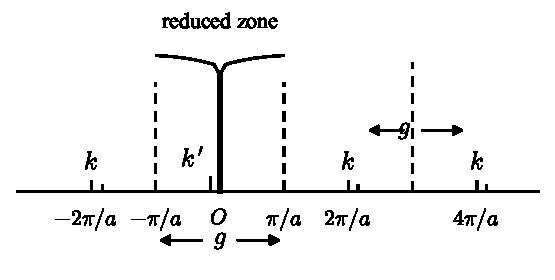
\includegraphics[width=0.72\textwidth]{fig_12.pdf}
\caption*{图 12\quad 诸点 $k$ 在一维倒格子中全都约化为 $k'$。}
\end{figure}

很自然地取 $k'$ 作为所有这些点的代表，且使 $|k'|$ 尽可能小。换句话说，我们总是选取落在范围
\begin{equation*}
-\frac{\pi}{a}<k\leqslant\frac{\pi}{a}.
\tag{1.68}
\end{equation*}
之内的值来作为波数。

显然，这个范围对我们的一维系统来说就等价于一个布里渊区；它是倒格子的一个晶胞。在三维情形我们如法炮制——我们选取波矢，使它落在倒格子空间的第一布里渊区内。这件事总是可能的，由初等几何即可明白。我们在式 (1.64) 中这样选取 $\mathbf{g}$ 的值，使 $|\mathbf{k}'|$ 尽可能小——也就是说，使它离倒格子的原点尽可能地近。这意味着 $|\mathbf{k}'|$ 所在之处离原点要比离倒格子的任何其他格点都近——这就等于说它落在该格子的Wigner–Seitz原胞内，也就是落在布里渊区内。显然，我们可以把倒格子空间中的任何一点 $\mathbf{k}$ \emph{约化}为布里渊区中的一点，于是任何态都可以在简约区图式（reduced zone scheme）中获得一个标记。

于是任何态都可以用它的简约波矢（reduced wave-vector）来表征。但可能有许多态具有同一个简约波矢而能量各不相同。因此，采用简约区图式使我们无法给每个态指定一个互不相同的 $\mathbf{k}$ 值。

\begin{figure}[H]
\centering
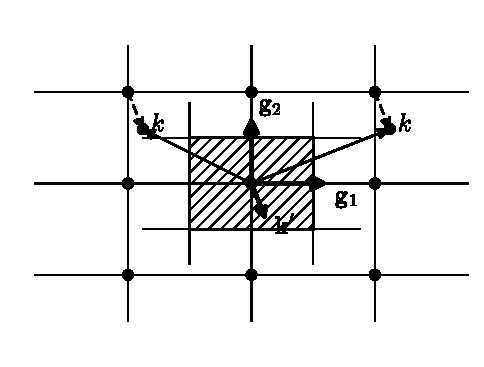
\includegraphics[width=0.72\textwidth]{fig_13.pdf}
\caption*{图 13\quad 诸波矢 $\mathbf{k}$ 全都约化为位于布里渊区中的 $\mathbf{k}'$。}
\end{figure}

看一看自由电子态在空晶格中会发生些什么，是很有意思的。设
\begin{align*}
\psi&=e^{i\mathbf{k}\cdot\mathbf{r}}\notag\\
&=e^{i(\mathbf{k}-\mathbf{g})\cdot\mathbf{r}}e^{i\mathbf{g}\cdot\mathbf{r}}\notag\\
&=e^{i\mathbf{k}'\cdot\mathbf{r}}\left(e^{i\mathbf{g}\cdot\mathbf{r}}\right),
\tag{1.69}
\end{align*}
其中 $\mathbf{k}'$ 是实际波矢 $\mathbf{k}$ 的约化值。这具有式 (1.60) 的形式，因为 $\exp(i\mathbf{g}\cdot\mathbf{r})$ 是晶格中的周期函数；但它是平面波的一种极其生硬人为的表示。如果在一维情形下能量由
\begin{equation*}
\mathcal{E}(\mathbf{k})=\frac{\hbar^{2}k^{2}}{2m},
\tag{1.70}
\end{equation*}
给出，那么在简约区中它将表现为 $\mathbf{k}'$ 的多值函数。在图 14 中，抛物线的 $AB$ 段经平移一个倒格矢被移到 $A'B'$ 处，如此等等。显然，在这种情形下，其中每个态都用它的“真实”波矢 $\mathbf{k}$ 来表示的扩展区图式（extended zone scheme）要更自然。

\section{边界条件：态的计数}

以上这一切都假定了完全的平移对称性，而这将要求晶格为无限。这在数学上相当麻烦，因为那样一来，原子和有待处理的态都会有无限多个。我们唯一的办法，是先处理一个原子数目有限的系统，然后令这个数目趋于无穷而取极限。我们也许会像对待真实表面那样引入边界，例如要求波函数在边界上必须为零。但这样做同样不便，因为此时系统的严格定态将不得不计及来自边界的所有反射，结果都会成为驻波。传导电子通常在极短的距离内就会被杂质或热振动非相干地散射开；要用这类函数去表示传导电子的态，在数学上笨拙，而且在本质上是不物理的。

\begin{figure}[H]
\centering
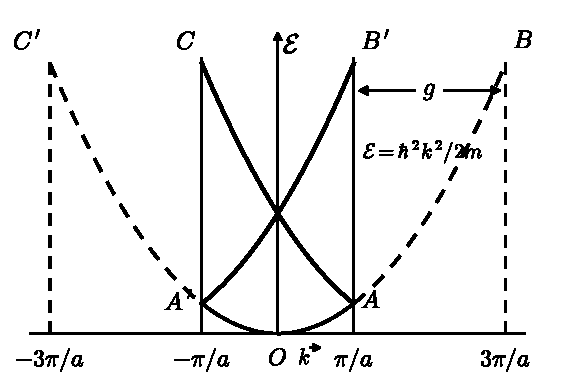
\includegraphics[width=0.72\textwidth]{fig_14.pdf}
\caption*{图 14\quad 简约区中自由电子的能量。}
\end{figure}

有一个数学上的手法，能圆满地解决态的计数问题，却又不会引入任何来自边界的直接物理效应。这就是采用循环（cyclic）边界条件，即 Born–von Kármán 边界条件。

在一维情形，设这个“晶体”含有 $L$ 个晶胞，它们首尾相接连成一个环。这一做法对电子波函数的后果，可以用如下条件来表达：
\begin{equation*}
\psi(x+La)=\psi(x),
\tag{1.71}
\end{equation*}
这就保证了在接合点处没有不连续。

但我们的一维 Bloch 条件给出
\begin{equation*}
\psi_k(x+La)=e^{ikLa}\psi_k(x),
\tag{1.72}
\end{equation*}
于是必须有
\begin{equation*}
e^{ikLa}=1,
\tag{1.73}
\end{equation*}
即
\begin{equation*}
k=\frac{2\pi m}{La},
\tag{1.74}
\end{equation*}
其中 $m$ 为整数。

在一维的简约区中，我们有 $-\pi/a<k\leqslant\pi/a$，因此落在范围
\begin{equation*}
-\frac{1}{2}L<m\leqslant\frac{1}{2}L
\tag{1.75}
\end{equation*}
之内的那些整数，将给出所有本质上不同的简约波数值。这样的值恰好有 $L$ 个（这里当然要分别处理 $L$ 为奇数和 $L$ 为偶数的不同情形——一个琐碎的细节），并且相邻两值相隔 $(1/L)(2\pi/a)$。由于假定 $L$ 非常大，这个分布实际上是连续的，并且在倒格子空间中具有恒定的密度。

在三维情形，我们把这一论证加以推广，宣称宏观系统在三个维度上都是循环的。我们把它取为沿晶格三个基矢方向尺寸分别为 $L_1\mathbf{a}_1$、$L_2\mathbf{a}_2$、$L_3\mathbf{a}_3$ 的晶体，并写下
\begin{equation*}
\psi(\mathbf{r}+L_1\mathbf{a}_1)=\psi(\mathbf{r}),\quad
\psi(\mathbf{r}+L_2\mathbf{a}_2)=\psi(\mathbf{r}),\quad
\psi(\mathbf{r}+L_3\mathbf{a}_3)=\psi(\mathbf{r}),
\tag{1.76}
\end{equation*}
正如式 (1.71) 一样。

对于波矢为 $\mathbf{k}$ 的 Bloch 态，这些条件意味着
\begin{equation*}
e^{i\mathbf{k}\cdot(L_1\mathbf{a}_1)}
=e^{i\mathbf{k}\cdot(L_2\mathbf{a}_2)}
=e^{i\mathbf{k}\cdot(L_3\mathbf{a}_3)}=1,
\tag{1.77}
\end{equation*}
而这只有当 $\mathbf{k}$ 取如下形式时方能实现：
\begin{align*}
\mathbf{k} &= k_1\mathbf{b}_1+k_2\mathbf{b}_2+k_3\mathbf{b}_3\\
&= \frac{2\pi m_1}{L_1}\mathbf{b}_1+\frac{2\pi m_2}{L_2}\mathbf{b}_2+\frac{2\pi m_3}{L_3}\mathbf{b}_3,
\tag{1.78}
\end{align*}
其中 $m_1$、$m_2$、$m_3$ 为整数，而矢量 $\mathbf{b}_1$、$\mathbf{b}_2$、$\mathbf{b}_3$ 当然就是 $(\mathbf{a}_1,\mathbf{a}_2,\mathbf{a}_3)$ 的倒格子三矢组（reciprocal triad），如式 (1.19) 中那样。

但这一结果显然可与倒格矢的定义相类比：
\begin{equation*}
\mathbf{g}=n_1\cdot 2\pi\mathbf{b}_1+n_2\cdot 2\pi\mathbf{b}_2+n_3\cdot 2\pi\mathbf{b}_3,
\tag{1.79}
\end{equation*}
其中 $n_1$、$n_2$、$n_3$ 为整数。把倒格子晶胞的生成矢量沿 $\mathbf{b}_1$ 方向分成 $L_1$ 份、沿 $\mathbf{b}_2$ 方向分成 $L_2$ 份、沿 $\mathbf{b}_3$ 方向分成 $L_3$ 份，便得到式 (1.78) 中 $\mathbf{k}$ 的允许值（allowed values）。于是，宛如生出一阵细密的疹点，点子均匀地布满倒格子空间，如图 15 所示。

要计算这些点的密度，只需注意到：让整数 $m_1$、$m_2$、$m_3$ 取遍
\begin{equation*}
0\leqslant m_1<L_1,\quad
0\leqslant m_2<L_2,\quad
0\leqslant m_3<L_3.
\tag{1.80}
\end{equation*}
即可铺满倒格子的一个晶胞。

但这并不是我们自然会选来作为 $\mathbf{k}$ 矢量基本区的晶胞。或许改取如下范围更好：
\begin{equation*}
-\frac{1}{2}L_1<m_1<\frac{1}{2}L_1,\quad
-\frac{1}{2}L_2<m_2<\frac{1}{2}L_2,\quad
-\frac{1}{2}L_3<m_3<\frac{1}{2}L_3,
\tag{1.81}
\end{equation*}
以与式 (1.75) 类比。这将给出一个以原点为中心的平行六面体晶胞。然而，晶胞的最佳选择是倒格子的 Wigner–Seitz 原胞，也就是我们的老朋友——布里渊区。

\begin{figure}[H]
\centering
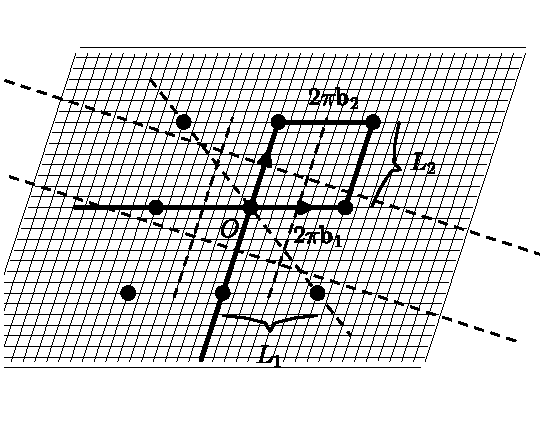
\includegraphics[width=0.72\textwidth]{fig_15.pdf}
\caption*{图 15\quad 布里渊区与倒格子的平行六面体晶胞覆盖相同的面积，且恰含 N 个“允许的 k 矢量”。}
\end{figure}

由于布里渊区的体积与平行六面体晶胞相同，它必定恰好含有同样数目的 $\mathbf{k}$ 的“允许值”。由式 (1.80) 或式 (1.81)，这个数目显然就是 $L_1\times L_2\times L_3=N$，而这正是我们整块宏观晶体中晶胞的数目。这是一个极其重要的定理：\emph{一块晶体中有多少个晶胞，一个布里渊区中就恰有多少个允许的波矢。}

我们已经证明过（式 (1.32)），一个区的体积为 $8\pi^3/v_c$。若体积为 $V$ 的晶体中有 $N$ 个晶胞，则
\begin{equation*}
v_c=V/N.
\tag{1.82}
\end{equation*}
于是，每个允许的 $\mathbf{k}$ 矢量在 $\mathbf{k}$ 空间中占据的体积便是
\begin{equation*}
\frac{1}{N}\,\frac{8\pi^3}{v_c}=\frac{8\pi^3}{V}.
\tag{1.83}
\end{equation*}
因此，\emph{倒格子空间单位体积内有 $V/8\pi^3$ 个允许的 $\mathbf{k}$ 矢量。}

实际上 $N$ 非常大，以致这一分布被当作连续分布来处理。我们常把对 $\mathbf{k}$ 矢量的求和写成一个积分
\begin{equation*}
\sum_{\mathbf{k}}\rightarrow\int d\mathbf{k}\equiv\frac{V}{8\pi^3}\iiint d^3k,
\tag{1.84}
\end{equation*}
这里用单个积分作为求和之极限的简明记号。然而，重要的是要记住：当我们真正要在 $\mathbf{k}$ 空间中做具体求积时，必须计入权重因子 $V/8\pi^3$。为简单起见，我们通常将假定 $V=1$，这时 $N$ 就是单位体积晶体中的晶胞数，而 $1/N$ 就是一个晶胞的体积。

结果 (1.83) 实际上不依赖于任何所假定的区结构；它在辐射理论中以及在自由电子情形下早已为人熟知。但就许多目的而言，布里渊区恰好含有 $N$ 个允许点这一事实更为有用。它表明这个区在本质上是不变的，仅依赖于晶体结构；增大整块晶体的尺寸，只会使 k 空间中的态密度（density of states）增大。

不过，必须承认，Born–von Kármán 条件在物理上是无法实现的。在二维情形，画在环面（torus）表面上的晶胞网络沿两个方向都是循环的；但对三维晶格来说，无论怎样施展拓扑上的扭曲，都无法使三个条件同时满足。尽管如此，它作为一种数学技巧用起来极为出色，而且可以用一些繁冗的数学来为它提供证明。事实是：在大量子数的渐近极限下，态密度对边界条件的具体形式非常不敏感。只要我们并不打算讨论边界效应本身，循环边界条件就远远是最方便的选择。

 % 本文件由 scripts/assemble.py 自动装配，勿手改（改 parts/ 后重跑）
% 第2章 格波

% 第2章 LATTICE WAVES

\chapter{格波}

\epigraphbook{那些井然有序的运动，那规整齐一的步伐，虽不给耳朵任何声息，却向理解之心敲出最为盈满和谐的音律。}{Sir Thomas Browne}

\section{晶格动力学}

最简单的固体大概要数固态氩：它是中性原子的规则排列，原子带着结合紧密的封闭电子壳层，靠 van der Waals 力维系在一起，这种力主要作用在晶格中最近邻的原子之间。这类晶体的物理学，就是原子在各自理想化平衡位置附近的热运动。

要讨论这种运动，最初等的观念是 \emph{Einstein 模型}（Einstein model）：每个原子都在其邻居的力场所形成的势阱中，像一个简谐振子那样振动。这个力场绝不会严格是一个具有球对称性的二次势阱，但就平均而言，这是一种合理的近似。于是，晶体的激发谱由间距为 $\hbar\nu_E$ 的能级组成，其中 $\nu_E$ 是 \emph{Einstein 频率}（Einstein frequency），即每个原子在其势阱中的振荡频率。

这个模型在某些只需对热振动作极粗略处理的场合是有用的——尤其是在相对高温时，此时各原子彼此独立地振动这一假设是站得住脚的。但我们一眼就能看出：若两个或更多的原子一致地运动，它们之间那种趋于把每个原子拉回平衡位置的力便会减弱，因而激发一个量子所需的能量可能要小得多。相邻原子的运动有一种相互关联的趋势。

要得到整个晶格的谱，我们必须把局域的力放进来，并对运动作完整的描述。若不是晶格具有平移不变性，这将是一个无法解决的问题。这些激发必须满足 Bloch 定理，正如 §1.4 中所证明的那样。\emph{晶格动力学}（lattice dynamics）的理论，为第 1 章中建立起来的整套数学机器提供了最初等的例子。

让我们先定义\emph{晶格位移}（lattice displacements）：$\mathbf{u}_{sl}$ 是这样一个矢量，它给出第 $l$ 个晶胞中第 $s$ 个原子离开其平衡位置的位移。设此原子的质量为 $M_s$，则系统的动能定义为
\begin{equation*}
\text{K.E.} = \sum_{sl} \frac{1}{2} M_s \left| \dot{\mathbf{u}}_{sl} \right|^2.
\tag{2.1}
\end{equation*}
我们在这里作相当普遍的假设：晶格是带基元的格子（lattice with a basis），因此标记 $s$ 遍取晶胞中的一个或多个原子。

至于势能一项，我们本需要把原子间的力定义出来。但我们可以相当普遍地假设，存在一个函数 $\mathcal{V}(\mathbf{u}_{sl})$，它用所有原子的位置——也就是说，用它们在某一时刻离开平衡晶格格点的实际位移——来表达整个晶体的势能。我们还可以进一步假设：当所有 $\mathbf{u}_{sl}$ 为零时，这个函数取极小，因为完整晶格想必是一个稳定平衡的组态。我们利用微振动理论，把 $\mathcal{V}$ 在这一点附近按 $\mathbf{u}_{sl}$ 的笛卡儿分量 $u_{sl}^{j}$ 展开成幂级数：
\begin{equation*}
\mathcal{V} = \mathcal{V}_0 + \sum_{slj} u_{sl}^{j} \left[ \frac{\partial \mathcal{V}}{\partial u_{sl}^{j}} \right]_0
+ \frac{1}{2} \sum_{ss',\,ll',\,jj'} u_{sl}^{j} u_{s'l'}^{j'} \left[ \frac{\partial^2 \mathcal{V}}{\partial u_{sl}^{j} \, \partial u_{s'l'}^{j'}} \right]_0 + \ldots
\tag{2.2}
\end{equation*}
常数项在当前的讨论里无关紧要；线性项的系数必须为零，因为我们处在平衡点附近；于是第一个重要的项必然是位移的二次项——即所谓的\emph{谐和项}（harmonic term）。

由这两个函数，即式 (2.1) 与式 (2.2)，用经典力学中通常的 Lagrange 程序，我们得到各分量的运动方程
\begin{equation*}
M_s \ddot{u}_{sl}^{j} = - \sum_{s'l'} \left[ \frac{\partial^2 \mathcal{V}}{\partial u_{sl}^{j} \, \partial u_{s'l'}^{j'}} \right]_0 u_{s'l'}^{j'}
\tag{2.3}
\end{equation*}
它对晶胞中所有的格点 $s$、对晶格中所有的晶胞 $l$、以及位移矢量的每一个笛卡儿分量 $j = x, y, z$ 都成立。

这些方程当然代表了数目极其庞大的耦合微分方程。但让我们考察一下右边的系数。令
\begin{equation*}
\left[ \frac{\partial^2 \mathcal{V}}{\partial u_{sl}^{j} \, \partial u_{s'l'}^{j'}} \right]_0 \equiv \mathsf{G}_{sl;s'l'}^{jj'}.
\tag{2.4}
\end{equation*}
这些系数构成一个笛卡儿张量的分量，于是我们可以把式 (2.3) 用矢量形式写得更简洁些：
\begin{equation*}
M_s \ddot{\mathbf{u}}_{sl} = - \sum_{s'l'} \mathsf{G}_{sl;s'l'} \cdot \mathbf{u}_{s'l'}.
\tag{2.5}
\end{equation*}

这个方程可以作如下解释：右边求和中的每一项，都是第 $l'$ 个晶胞中第 $s'$ 个格点上的原子因位移 $\mathbf{u}_{s'l'}$ 而\emph{作用在第 $l$ 个晶胞中第 $s$ 个原子上的力}。倘若我们知道整个晶格的势能可以由原子对之间的力构造出来，那就可以直接用原子间力常数把它写出来。

但无论这些力的物理图像如何，有一点是必需的：它们不能依赖于 $l$ 和 $l'$ 在晶格中的绝对位置。张量 $\mathsf{G}$ 必须只是它们相对位置的函数：
\begin{equation*}
\mathsf{G}_{sl;s'l'} = \mathsf{G}_{ss'}(\boldsymbol{h}), \quad \text{其中}\ \ \boldsymbol{h} = \boldsymbol{l}' - \boldsymbol{l}.
\tag{2.6}
\end{equation*}
我们的运动方程现在读作
\begin{equation*}
M_s \ddot{\mathbf{u}}_{sl} = - \sum_{s'\boldsymbol{h}} \mathsf{G}_{ss'}(\boldsymbol{h}) \cdot \mathbf{u}_{s,\,l+\boldsymbol{h}}.
\tag{2.7}
\end{equation*}

这些方程具有满足 Bloch 定理所要求的平移不变的形式；把标记从 $l$ 换成譬如 $l''$，只不过是原封不动地重复同一组方程。现在假设我们已经找到了一个解——一组描述各个 $l$ 值的 $\mathbf{u}_{sl}$ 的时间函数。这些函数必须满足 Bloch 条件 (1.48) 或 (1.57)。于是存在一个波矢\footnote{我们用这个符号表示格波的波矢，而用 $\boldsymbol{k}$ 表示电子波的波矢。当然，二者都是同一倒格子空间中的矢量。}$\boldsymbol{q}$，使得
\begin{equation*}
\mathbf{u}_{sl}(t) = e^{i\boldsymbol{q}\cdot\boldsymbol{l}} \mathbf{u}_{s,o}(t),
\tag{2.8}
\end{equation*}
其中 $\mathbf{u}_{s,o}(t)$ 是碰巧被选作格矢 $\boldsymbol{l}$ 原点的那一晶胞处的位移。注意：在每一个晶胞里，格点 $s$ 上的原子都以相同的振幅沿相同的方向运动；逐胞不同的只是相位。

动力学方程的每一个解，都有一个使式 (2.8) 得以满足的 $\boldsymbol{q}$ 值。要弄清哪个解带哪个波矢，我们必须回到式 (2.7)。把式 (2.8) 代入，得
\begin{equation*}
M_s \ddot{\mathbf{u}}_{s,o}\, e^{i\boldsymbol{q}\cdot\boldsymbol{l}} = - \sum_{s'\boldsymbol{h}} \mathsf{G}_{ss'}(\boldsymbol{h}) \cdot \mathbf{u}_{s',o}\, e^{i\boldsymbol{q}\cdot\boldsymbol{h}} e^{i\boldsymbol{q}\cdot\boldsymbol{l}}.
\tag{2.9}
\end{equation*}
因子 $\exp i\boldsymbol{q}\cdot\boldsymbol{l}$ 可以消去。为了表明原点的选取完全任意，而我们处理的乃是具有确定 $\boldsymbol{q}$ 值的一个解，让我们写
\begin{equation*}
\mathbf{u}_{s,o} = \mathbf{U}_{s,\boldsymbol{q}}.
\tag{2.10}
\end{equation*}

于是只剩下
\begin{align*}
M_s \ddot{\mathbf{U}}_{s,\boldsymbol{q}} &= - \sum_{s'} \Bigl\{ \sum_{\boldsymbol{h}} \mathsf{G}_{ss'}(\boldsymbol{h})\, e^{i\boldsymbol{q}\cdot\boldsymbol{h}} \Bigr\} \cdot \mathbf{U}_{s',\boldsymbol{q}} \\
&= - \sum_{s'} \mathsf{G}_{ss'}(\boldsymbol{q}) \cdot \mathbf{U}_{s',\boldsymbol{q}},
\tag{2.11}
\end{align*}
其中
\begin{equation*}
\mathsf{G}_{ss'}(\boldsymbol{q}) \equiv \sum_{\boldsymbol{h}} \mathsf{G}_{ss'}(\boldsymbol{h})\, e^{i\boldsymbol{q}\cdot\boldsymbol{h}}
\tag{2.12}
\end{equation*}
——它是力张量（force tensor）$\mathsf{G}$ 的一个 Fourier 变换。

新方程组 (2.11) 相对而言容易求解。关键在于它的数目是有限的。设每个晶胞含 $n$ 个原子，晶格共有 $N$ 个晶胞。原来的方程组 (2.3) 或 (2.5) 将有 $3nN$ 个——这里对矢量的三个笛卡儿分量是分别计算的。而新方程组 (2.11) 只有 $3n$ 个——$n$ 个 $s$ 值的每一个各有 3 个分量方程。

这是平移不变性的一个极有威力的例证。所有晶胞在结构上本质同一，这意味着我们只需要关于其中一个晶胞的信息，就能计算整个集合的动力学。诚然，若想为每个 $\boldsymbol{q}$ 值（边界条件恰好允许 $N$ 个不同的值）求得解，我们得分别计算；但在实践中我们只关心这类解的一个有限样本，其余的可以靠插值得到。

接下来的步骤是初等的。如同在通常的振动理论中那样，我们假设 $\mathbf{U}_{s,\boldsymbol{q}}$ 含有时间因子 $\exp(i\nu t)$。于是必须求解由 $3n$ 个方程组成的方程组
\begin{equation*}
\sum_{s'j'} \Bigl\{ \mathsf{G}_{ss'}^{jj'}(\boldsymbol{q}) - \nu^2 M_s \delta_{ss'} \delta_{jj'} \Bigr\} U_{s',\boldsymbol{q}}^{j'} = 0,
\tag{2.13}
\end{equation*}
其未知对象是 $\mathbf{U}_{s,\boldsymbol{q}}$ 的各分量。这是一个本征值方程；令矩阵 $\{\ \}$ 的行列式为零，得到一个关于 $\nu^2$ 的方程，求出它的根，便得到全部 $3n$ 个解。实际上，我们所做的无非是求出晶胞内 $n$ 个原子的 $3n$ 个简正模（normal mode）振动，只是假定它们通过力张量 $\mathsf{G}_{ss'}(\boldsymbol{q})$ 相互作用。这个张量不同于原来的原子间力张量 $\mathsf{G}_{ss'}(\boldsymbol{h})$，而且对每个 $\boldsymbol{q}$ 值都不相同；对给定的 $s$ 和 $s'$，它把晶格中每个晶胞的格点 $s$ 上的\emph{所有} $s$ 类原子（即每个晶胞中位于格点 $s$ 上的那些原子）与格点 $s'$ 上的\emph{所有}原子之间的相互作用总括起来，并计及它们之间的相对相位。

\section{格波的性质}

要理解格波的物理性质，研究几个简单的例子是有益的。其中最简单的当属\emph{线性链}（linear chain）。

假设我们有一维“晶格”，每个晶胞一个原子，且只有最近邻力。运动方程很容易写出来。势能（参见式 (2.2)）具有如下形式：
\begin{equation*}
\mathcal{V} = \sum_{l} \frac{1}{2} \alpha \left( u_{l} - u_{l+a} \right)^2,
\tag{2.14}
\end{equation*}
其中 $\alpha$ 是力常数（force constant）。运动方程（参见式 (2.5)）变为
\begin{equation*}
M \ddot{u}_{l} = - \alpha \left( 2u_{l} - u_{l+a} - u_{l-a} \right)
\tag{2.15}
\end{equation*}

\begin{figure}[H]
\centering
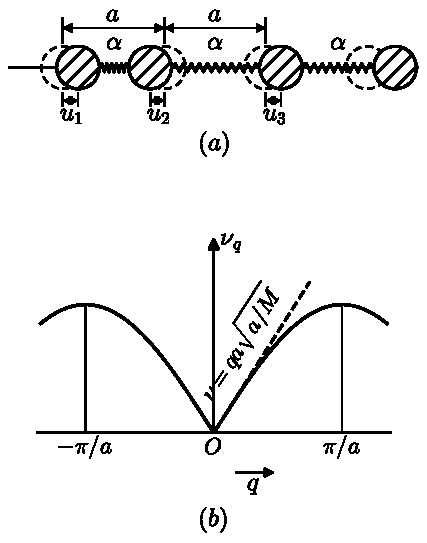
\includegraphics[width=0.72\textwidth]{fig_16.pdf}
\caption*{图 16\quad 线性链的振动频率}
\end{figure}

通过代换
\begin{equation*}
u_{l} = U_{q}\, e^{iql},
\tag{2.16}
\end{equation*}
它变换成与式 (2.11) 类比的方程，即
\begin{align*}
M \ddot{U}_{q} &= - \left( 2\alpha - \alpha e^{iqa} - \alpha e^{-iqa} \right) U_{q} \\
&= - 2\alpha \left( 1 - \cos qa \right) U_{q},
\tag{2.17}
\end{align*}
其中 $a$ 是链中原子的间距。这是一个简谐振子的方程，其频率为
\begin{equation*}
\nu_{q} = \sqrt{\left( \frac{\alpha}{M} \right)}\, 2 \sin \left( \frac{qa}{2} \right).
\tag{2.18}
\end{equation*}

这个众所周知的结果体现了理论的许多要点。（i）一切可能的振动，由如下范围内的 $q$ 值给出：
\begin{equation*}
- \frac{\pi}{a} < q \leqslant \frac{\pi}{a}.
\tag{2.19}
\end{equation*}
这正是我们的布里渊区（Brillouin zone）。任何落在这个范围之外的 $q$ 值都只是精确地重复同一运动：
\begin{equation*}
u_{l} = U\, e^{i(q+\sigma)l} \equiv U\, e^{iql}.
\tag{2.20}
\end{equation*}
把波矢取在布里渊区之外是相当不自然的（尽管并非没有意义！）。不过，假如我们当初用了大于 $\pi/a$ 的 $|q|$ 值，其实也会得到正确的结果。在式 (2.18) 中，$\nu_q$ 是 $q$ 的周期函数，所以凡在布里渊区内约化到同一点的那些 $q$ 值都具有相同的频率。

恰好有 $N$ 个不同的解，对应于布里渊区中 $N$ 个允许的 $q$ 值。这与原晶格的 $N$ 个自由度正相一致。

（ii）对于小的 $q$ 值（即 $qa \ll 1$），
\begin{equation*}
\nu_{q} \sim \sqrt{\left( \frac{\alpha}{M} \right)}\, aq.
\tag{2.21}
\end{equation*}

频率与波数成正比，这对应于连续介质中普通弹性波的一个众所周知的性质：若扰动的波长远大于晶格常数，那么这条原子链在经典力学中的行为就像一根“重弹性绳”。

然而在大的 $q$ 值处，波的速度不再是常数；到了 $q = \pi/a$，即波长等于 $2a$ 时，函数 $\nu_q$ 弯折下来趋于一条水平切线。这表现出\emph{色散}（dispersion）性质。

现在考虑一个更复杂的情形：一条原子线性链，间距和力常数都与前面相同，但两种不同的质量 $M_1$ 与 $M_2$ 交替排列。现在我们的晶胞含两个原子。与式 (2.11) 类比的方程要比式 (2.17) 复杂：
\begin{equation*}
\left.
\begin{aligned}
M_1 \ddot{U}_{1} &= - 2\alpha U_{1} + 2\alpha \cos qa \cdot U_{2}, \\
M_2 \ddot{U}_{2} &= - 2\alpha U_{2} + 2\alpha \cos qa \cdot U_{1}.
\end{aligned}
\right\}
\tag{2.22}
\end{equation*}

为求频率 $\nu$，我们必须求解行列式方程
\begin{equation*}
\begin{vmatrix}
2\alpha - M_1 \nu^2 &\quad - 2\alpha \cos qa \\
- 2\alpha \cos qa &\quad 2\alpha - M_2 \nu^2
\end{vmatrix} = 0,
\tag{2.23}
\end{equation*}
它有两个根
\begin{equation*}
\nu_{\pm}^{2} = \alpha \left( \frac{1}{M_1} + \frac{1}{M_2} \right) \pm \alpha \sqrt{\left\{ \left( \frac{1}{M_1} + \frac{1}{M_2} \right)^{2} - \frac{4 \sin^{2} qa}{M_1 M_2} \right\}}.
\tag{2.24}
\end{equation*}
把这两个根作为 $q$ 的函数描画出来，就如图 18 所示。

\begin{figure}[H]
\centering
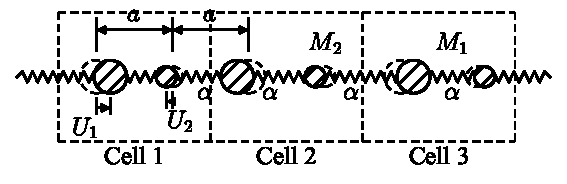
\includegraphics[width=0.72\textwidth]{fig_17.pdf}
\caption*{图 17\quad 双原子线性链}
\end{figure}

\begin{figure}[H]
\centering
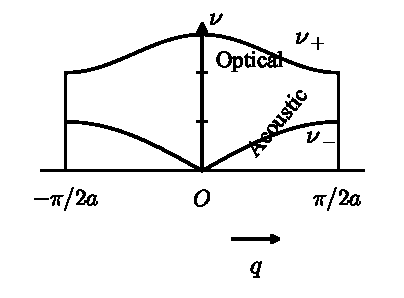
\includegraphics[width=0.72\textwidth]{fig_18.pdf}
\caption*{图 18\quad 双原子链的振动频率}
\end{figure}

与单原子链一样，这里有一个根 $\nu_{-}$，它在 $q = 0$ 附近趋于与 $q$ 成正比。我们称之为\emph{声学支}（acoustic mode），因为它是把链当作弹性连续体时的长波长振动的对应物。这种情形下求出的声速正是这种介质中正常的声速——我们把这个证明留作读者的练习。

但还有另一个分支 $\nu_{+}$，在 $q = 0$ 附近满足
\begin{equation*}
\nu_{+}^{2} \sim 2\alpha \left( \frac{1}{M_1} + \frac{1}{M_2} \right)
\tag{2.25}
\end{equation*}
这个分支与声学支相隔甚远，但随着 $q$ 的增大，两个分支的频率有相互靠近的趋势。这叫做\emph{光学支}（optical mode）。我们容易验证：在 $q = 0$ 的情形，轻、重两类原子各自的子晶格（sublattice）都在作刚体式的整体运动，且两者彼此反向；或者可以这样说，每个晶胞里的双原子分子都在振动，仿佛与邻居无关。如果像在离子晶体中那样，两类原子带有异号电荷，这就给出一个振荡的偶极矩，因而是光学活性的。

\begin{figure}[H]
\centering
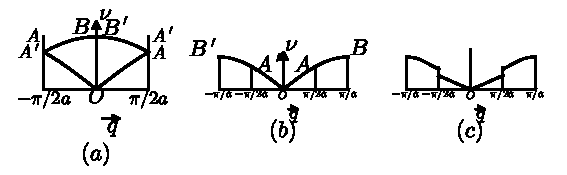
\includegraphics[width=0.72\textwidth]{fig_19.pdf}
\caption*{图 19\quad 振动频率：(a) 按双原子链处理的单原子线性链；(b) 单原子线性链，显示区边界；(c) 按单原子链处理的双原子线性链}
\end{figure}

研究从图 16 的单原子链到图 18 的双原子链的转变，是很有启发性的。假设我们在第一种情形下一开始就取一个含两个原子的晶胞，而无视这两个原子质量相同的事实。容易证明：此时光学支与声学支将在 $q = \pi/2a$ 处相接，如图 19(a) 所示。与图 16 相比，我们似乎把模的数目加倍了。然而，晶胞长度加倍之后，布里渊区的尺寸显然减半了。通过平移 $\pi/a$（即对我们这个加倍后的晶胞而言的一个倒格矢），可以把图 19(a) 展开成图 19(b)。这时“声学”支与“光学”支便连续相接。图 19(a) 的简约区是虚假地只及应有大小的一半。

我们可以换一种说法。交替改变链上原子的质量，其效果是在 $\pm \pi/2a$ 处引入新的区边界。频率跨越这条边界不再连续；出现了一个隙。我们可以用图 19(c) 来表示——这是处理双原子链的另一种方式。在下一章里我们会经常遇到这个现象。

下一个要考虑的情形，该是具有最近邻相互作用的二维或三维 Bravais 格子。然而这时方程已经复杂得难以轻松地一般求解。每一个维度都给位移矢量引入一个额外的笛卡儿分量，因此在三维情形我们必须求解一个关于 $\nu^2$ 的三次方程。

在这种情形下，只要过渡到长波极限，这三个根就可以在物理上加以辨认。实际上我们处理的是一个弹性连续体，其结构过于细微，在长波的动力学中无足轻重。众所周知，在这样的连续体中可以传播三种不同类型、速度各不相同的声波。

\begin{figure}[H]
\centering
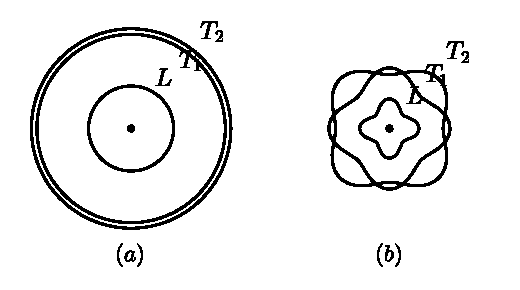
\includegraphics[width=0.72\textwidth]{fig_20.pdf}
\caption*{图 20\quad 恒定频率面：(a) 各向同性介质；(b) 真实晶体}
\end{figure}

这三个\emph{声学支}的本质差别在于它们的\emph{偏振}（polarization）性质。例如在各向同性连续体中，有一个模是\emph{纵}偏振的——每个原子的位移矢量都沿着波的传播方向。另外两个模速度相同，是\emph{横}偏振的——原子在垂直于波矢的平面内运动。一般说来，纵模的速度比横模高，因此 $\boldsymbol{q}$ 空间中的恒定频率面看上去就像图 20(a) 那样。

晶体固体在宏观弹性性质上通常不是各向同性的，所以这幅图像会引人误解。给定类型的波，其速度将依赖于传播方向。于是（图 20(b)）横支的恒定频率面可能离球面很远。这样，除了特殊的对称方向之外，两个横模将不再简并，它们的频率面可能以复杂的样式相互交截。的确，把模形式上分成横模与纵模是有点误导的：在这样的介质中，实际的偏振矢量（即方程 (2.11) 或 (2.13) 的解矢量 $\mathbf{U}_{\boldsymbol{q}}$ 的方向）未必严格地平行或垂直于 $\boldsymbol{q}$。

由此，格波的长波行为就确定下来了。对沿给定方向的 $\boldsymbol{q}$，我们必须有 $\nu$ 与 $q$ 之间的一个关系，其形式如图 21 所勾勒——在 $q = 0$ 附近是线性关系，斜率等于相应的宏观声速。但随着 $q$ 增大，我们逼近布里渊区的边界，就必定出现色散。

\begin{figure}[H]
\centering
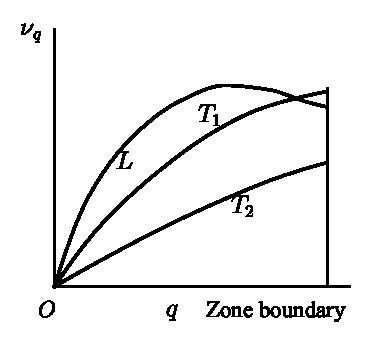
\includegraphics[width=0.72\textwidth]{fig_21.pdf}
\caption*{图 21\quad 格波在给定方向上的色散}
\end{figure}

此后的确切行为会相当复杂。一般地说，$\nu_{\boldsymbol{q}}$ 会像线性情形那样弯折下来，但不一定弯到水平切线。唯一的规则是：$\nu_{\boldsymbol{q}}$ 作为倒格子空间中 $\boldsymbol{q}$ 的函数，其根的整体图样是连续的，并且具有倒格子的周期性。察看式 (2.8) 与式 (2.12) 即可明白这一点。与线性情形一样，若 $\boldsymbol{g}$ 是一个倒格矢，则波矢 $\boldsymbol{q}' = \boldsymbol{q} + \boldsymbol{g}$ 的解与波矢 $\boldsymbol{q}$ 的解完全相同，所以 $\nu_{\boldsymbol{q}}$ 以 $\boldsymbol{g}$ 为周期。它是 $\boldsymbol{q}$ 空间中的连续函数，因为它是一个本征值方程的解，该方程的矩阵是对称的，而其系数本身就是 $\boldsymbol{q}$ 空间中的连续周期函数。

这意味着，当我们把像图 20(b) 那样的图形扩展到整个区时，它必定构成这种图样的一部分，如图 22 所草示。只要知道力常数，这样的图是能够计算出来的——尽管在实践中更常见的做法是：先用中子或 X 射线衍射（参见 §2.8）测定各方向上的色散曲线，再反过来寻找能与之拟合的原子力常数。

在带基元的三维晶格这一更复杂的情形，我们还会发现横光学支与纵光学支，它们各有自己的色散曲线和能量面。所有这些情形，原则上都涵盖在我们的普遍方程 (2.13) 之中。

%（以下为 §2.2 收尾的插图，印于书页 37 顶部，随图移归上一部分 A）
\begin{figure}[H]
\centering
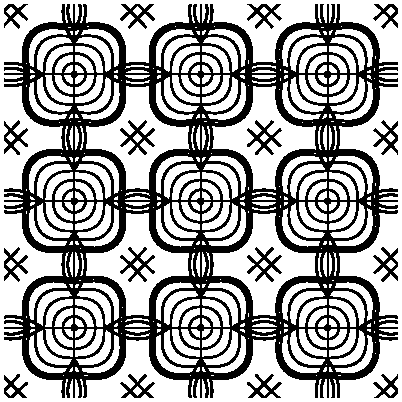
\includegraphics[width=0.72\textwidth]{fig_22.pdf}
\caption*{图 22\quad 重复区图式（repeated zone scheme）下晶格频率函数的一支 $\nu_{\mathbf{q}}$}
\end{figure}

\section{晶格求和}

在长波极限下，晶格简正模方程的解与宏观连续介质弹性波方程的解之间的等价性，为把原子力常数同固体中观测到的弹性常数联系起来提供了一个便利的方法。原则上这是一个比较简单的纲领，尽管在实践中它可能涉及繁冗的计算。

有一个主要的困难之处。在一个常见的情形中，我们对原子间力了解得非常清楚：在离子晶体中，固体内聚能的主要部分来自异号电荷离子之间的 Coulomb 力。例如，对于位于诸点 $\mathbf{R}_l$ 处的一组离子，总静电能必定由
\begin{equation*}
\mathcal{E} = \frac{1}{2}\sum_{ij} \frac{\pm e^2}{|\mathbf{R}_i - \mathbf{R}_j|}
\tag{2.26}
\end{equation*}
给出，正负号取决于 $\mathbf{R}_i$ 与 $\mathbf{R}_j$ 两处电荷的相对符号。

此式可以改写成
\begin{equation*}
\mathcal{E} = -\frac{1}{2}N\alpha\,\frac{e^2}{a},
\tag{2.27}
\end{equation*}
其中 $a$ 是一个晶格常数，系数 $\alpha$ 现在是无量纲的，依赖于正、负离子在晶格中的排布方式。这样，\emph{Madelung 常数} $\alpha$ 作为表征某一特定类型晶体结构的参量（而不管其尺度大小），就有了一定的意义。

\begin{figure}[H]
\centering
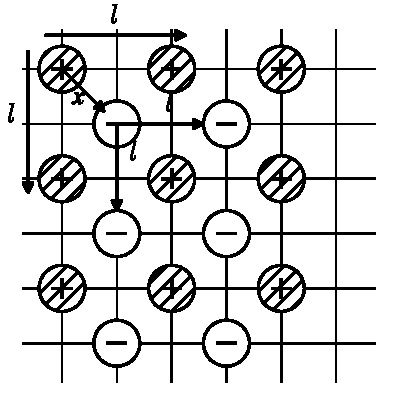
\includegraphics[width=0.72\textwidth]{fig_23.pdf}
\caption*{图 23\quad （原书此图无图注）}
\end{figure}

例如，设我们的离子晶体由两套子晶格组成——正离子位于一组格点 $\boldsymbol{l}$ 上，负离子位于 $\boldsymbol{l}+\mathbf{x}$ 上。我们需要计算
\begin{equation*}
\alpha = a\sum_{\boldsymbol{l}}\left\{\frac{1}{|\boldsymbol{l}|} - \frac{1}{|\boldsymbol{l}+\mathbf{x}|}\right\}
\tag{2.28}
\end{equation*}
（第一项中除去 $\boldsymbol{l}=0$）。麻烦在于，这个和式中的两项分开来各自发散；在距离 $\boldsymbol{l}$ 处，有待计入的点的数目是 $l^2$ 的量级。

这个级数是条件收敛的，而且即使如此，收敛也很慢。计算这类和式的问题变得十分严峻。最好的直接方法是 Evjen 方法，即从原点向外逐个处理各层壳，使每一壳的总静电电荷恰好为零。

这个困难并不只限于内聚能的计算。在计算诸如式 (2.12) 那样的表达式——原子之间力张量的 Fourier 变换——时也会出现。在那里，我们同样要对所有格点求和，而对 Coulomb 力来说收敛很慢。任何计算离子晶体晶格动力学的尝试都必然碰上这个困难。

有一个非常漂亮的方法，称为 \emph{Ewald 方法}（Ewald's method），可以用它解决这个问题。也许这只是一个技巧，算不上固体理论的一条基本原理，但它实在精巧，值得稍作题外的讨论。它还演示了晶格上周期函数理论的某些内容。

先考虑函数
\begin{equation*}
\frac{2}{\sqrt{\pi}}\sum_{\boldsymbol{l}} e^{-|\boldsymbol{l}-\mathbf{r}|^2\rho^2} = F(\mathbf{r},\rho).
\tag{2.29}
\end{equation*}
这个函数在 $\mathbf{r}$ 中是周期的，具有晶格的周期性。因此，按式 (1.15)，可以把它展开成 Fourier 级数
\begin{equation*}
F(\mathbf{r},\rho) = \sum_{\boldsymbol{g}} F_{\boldsymbol{g}}\, e^{i\boldsymbol{g}\cdot\mathbf{r}},
\tag{2.30}
\end{equation*}
其中
\begin{equation*}
F_{\boldsymbol{g}} = \frac{1}{V}\int \frac{2}{\sqrt{\pi}}\sum_{\boldsymbol{l}} e^{-|\boldsymbol{l}-\mathbf{r}|^2\rho^2}\, e^{-i\boldsymbol{g}\cdot\mathbf{r}}\, d\mathbf{r},
\tag{2.31}
\end{equation*}
如式 (1.22)（积分遍及整个晶体）。

现在我们在级数的每一项中引入一个因子 $\exp(i\boldsymbol{g}\cdot\boldsymbol{l})=1$。这样一来，
\begin{align*}
F_{\boldsymbol{g}} &= \frac{1}{V}\,\frac{2}{\sqrt{\pi}}\sum_{\boldsymbol{l}}\int e^{-|\boldsymbol{l}-\mathbf{r}|^2\rho^2}\, e^{-i\boldsymbol{g}\cdot(\mathbf{r}-\boldsymbol{l})}\, d\mathbf{r} \\
&= \frac{N}{V}\,\frac{2}{\sqrt{\pi}}\int e^{-r^2\rho^2-i\boldsymbol{g}\cdot\mathbf{r}}\, d\mathbf{r},
\tag{2.32}
\end{align*}
因为和式中的每一项现在都相同，只不过各自取晶格中不同的点 $\boldsymbol{l}$ 为原点来计算。由于积分收敛很快，而所有格点又彼此等价，这一步是显而易见的。

式 (2.32) 中的积分很容易算出。它给出
\begin{equation*}
F_{\boldsymbol{g}} = \frac{2\pi}{v_c}\,\frac{1}{\rho^3}\, e^{-g^2/4\rho^2}.
\tag{2.33}
\end{equation*}
把式 (2.33) 代入式 (2.29) 和 (2.30)，得到的关系式在纯数学中称为 \emph{$\theta$ 函数变换}（theta-function transformation）（在纯数学中通常只对简单立方格子证明这个关系；我们的结果更为普遍）
\begin{equation*}
\frac{2}{\sqrt{\pi}}\sum_{\boldsymbol{l}} e^{-|\boldsymbol{l}-\mathbf{r}|^2\rho^2} = \frac{2\pi}{v_c}\sum_{\boldsymbol{g}}\frac{1}{\rho^3}\, e^{-g^2/4\rho^2}\, e^{i\boldsymbol{g}\cdot\mathbf{r}}.
\tag{2.34}
\end{equation*}
但是考虑恒等式
\begin{equation*}
\frac{2}{\sqrt{\pi}}\int_0^\infty e^{-z^2\rho^2}\, d\rho = \frac{1}{|z|}.
\tag{2.35}
\end{equation*}
把它用到式 (2.34) 的左端，我们有
\begin{equation*}
\sum_{\boldsymbol{l}}\frac{1}{|\boldsymbol{l}-\mathbf{r}|} = \sum_{\boldsymbol{l}}\frac{2}{\sqrt{\pi}}\int_0^\infty e^{-|\boldsymbol{l}-\mathbf{r}|^2\rho^2}\, d\rho.
\tag{2.36}
\end{equation*}
我们把对哑变量 $\rho$ 的积分在某个任意点 $G$ 处分成两部分，并在第一部分中用式 (2.34) 代换被积函数：
\begin{align*}
\sum_{\boldsymbol{l}}\frac{1}{|\boldsymbol{l}-\mathbf{r}|} &= \frac{2\pi}{v_c}\int_0^G \sum_{\boldsymbol{g}}\frac{1}{\rho^3}\, e^{-g^2/4\rho^2}\, e^{i\boldsymbol{g}\cdot\mathbf{r}}\, d\rho + \sum_{\boldsymbol{l}}\frac{2}{\sqrt{\pi}}\int_G^\infty e^{-|\boldsymbol{l}-\mathbf{r}|^2\rho^2}\, d\rho \\
&= \frac{\pi}{v_c}\,\frac{1}{G^2}\sum_{\boldsymbol{g}} e^{i\boldsymbol{g}\cdot\mathbf{r}}\,\frac{e^{-g^2/4G^2}}{g^2/4G^2} + \sum_{\boldsymbol{l}}\frac{1}{|\boldsymbol{l}-\mathbf{r}|}\,\mathrm{erfc}\{G|\boldsymbol{l}-\mathbf{r}|\},
\tag{2.37}
\end{align*}
其中第二项含有\emph{余误差函数}（complementary error function），当自变量取大值时它迅速趋于零。

具体做法是选取一个 $G$ 值，使得对 $\boldsymbol{l}$ 的级数和对 $\boldsymbol{g}$ 的级数都迅速收敛；容易看出，这两个级数都比原来的级数 (2.36) 收敛得好得多。从“物理上”讲，这就好像我们分两步在 $\mathbf{r}$ 处建立起电荷。第一步，我们作一个球对称的 Gaussian 分布，其在半径 $z$ 处的电荷密度正比于 $\exp(-G^2z^2)$。点电荷晶格与这个电荷云在长距离上的静电相互作用，给出式 (2.37) 中的第一项。然后我们再作修正：在 $\mathbf{r}$ 处放一个点电荷，同时减去 Gaussian 分布。这个对象是电中性的，它与晶格的长程相互作用可以忽略，只贡献一个对邻近格点迅速收敛的和。

不过事情还没有完，因为上面的和式全部取正号，而且当 $\mathbf{r}=0$ 时它包含了原点处的电荷对自身的作用。这会表现为第二个求和中 $\boldsymbol{l}=0$ 那一项在 $\mathbf{r}=0$ 附近的一个发散贡献。我们从左端的级数中减去 $1/r$，这等价于把右端对 $\boldsymbol{l}$ 求和中的第一项去掉，而在 $r\to 0$ 的极限下代之以下式
\begin{align*}
\frac{1}{r}\,\mathrm{erf}\,Gr - \frac{1}{r} &= \frac{2}{\sqrt{\pi}}\,\frac{1}{r}\left\{\int_{Gr}^{\infty} e^{-z^2}\, dz - \frac{\sqrt{\pi}}{2}\right\} \\
&= -\frac{2}{\sqrt{\pi}}\,\frac{1}{r}\int_0^{Gr} e^{-z^2}\, dz \\
&\to -2G/\sqrt{\pi}.
\tag{2.38}
\end{align*}
于是
\begin{equation*}
\sum_{\boldsymbol{l}\neq 0}\frac{1}{|\boldsymbol{l}|} = \frac{\pi}{v_c}\,\frac{1}{G^2}\sum_{\boldsymbol{g}}\frac{e^{-g^2/4G^2}}{g^2/4G^2} + \sum_{\boldsymbol{l}\neq 0}\frac{1}{|\boldsymbol{l}|}\,\mathrm{erf}\{G|\boldsymbol{l}|\} - \frac{2G}{\sqrt{\pi}}.
\tag{2.39}
\end{equation*}
式 (2.37) 和 (2.39) 都还含有一个奇异性；$\boldsymbol{g}=0$ 的项是发散的。但当我们像式 (2.28) 那样计算 Madelung 常数时，是从一个级数中减去另一个级数，两个奇异性便相互抵消。这说白了就是：每一套子晶格各自的平均势如果单独计算将是无穷大，但晶体的总电荷为零。

从这里我们可以看到这一变换的某种物理意义。考虑一个更复杂的情形。设有一个格波，在晶格的每个格点上产生一个偶极子，
\begin{equation*}
\mathbf{p}(\boldsymbol{l}) = \mathbf{p}\, e^{i\mathbf{q}\cdot\boldsymbol{l}}.
\tag{2.40}
\end{equation*}
由初等静电学可知，这组电荷分布在 $\mathbf{r}$ 处产生的 Coulomb 场，就是这些偶极子所产生的势的梯度：
\begin{align*}
\mathbf{E}(\mathbf{r}) &= \nabla\left\{\sum_{\boldsymbol{l}} \mathbf{p}(\boldsymbol{l})\cdot\nabla\left(\frac{1}{|\boldsymbol{l}-\mathbf{r}|}\right)\right\} \\
&= \nabla(\mathbf{p}\cdot\nabla)\left\{\sum_{\boldsymbol{l}} \frac{e^{i\mathbf{q}\cdot\boldsymbol{l}}}{|\boldsymbol{l}-\mathbf{r}|}\right\}.
\tag{2.41}
\end{align*}
对格点的这个和式是式 (2.36) 稍微复杂一点的版本。用我们上面在 $\mathbf{q}=0$ 的特殊情形中用过的同一套论证就可以把它求出来；结果是
\begin{equation*}
\sum_{\boldsymbol{l}} \frac{e^{i\mathbf{q}\cdot\boldsymbol{l}}}{|\boldsymbol{l}-\mathbf{r}|} = \frac{\pi}{v_c}\,\frac{1}{G^2}\sum_{\boldsymbol{g}} \frac{e^{i(\mathbf{q}+\boldsymbol{g})\cdot\mathbf{r}}\, e^{-|\mathbf{q}+\boldsymbol{g}|^2/4G^2}}{|\mathbf{q}+\boldsymbol{g}|^2/4G^2} + \sum_{\boldsymbol{l}} \frac{e^{i\mathbf{q}\cdot\boldsymbol{l}}}{|\boldsymbol{l}-\mathbf{r}|}\,\mathrm{erf}\{G|\boldsymbol{l}-\mathbf{r}|\},
\tag{2.42}
\end{equation*}
它可以逐项微商，正是式 (2.41) 所需要的。事实上，当离子之间存在 Coulomb 力时，我们在这里得到的就是计算力张量系数（如式 (2.12)）所需的那类公式。

但是考虑第一个求和中 $\boldsymbol{g}=0$ 那一项对电场的贡献：
\begin{equation*}
\mathbf{E}_0(\mathbf{r}) = \frac{-4\pi}{v_c}\, e^{-q^2/4G^2}\,\frac{(\mathbf{p}\cdot\mathbf{q})}{q^2}\,\mathbf{q}.
\tag{2.43}
\end{equation*}
除了因子 $\exp(-q^2/4G^2)$ 之外，这正是宏观电场 $\overline{\mathbf{E}}(\mathbf{r})$，即与下述宏观极化波
\begin{equation*}
\mathbf{p}(\mathbf{r}) = \mathbf{p}\, e^{i\mathbf{q}\cdot\mathbf{r}}
\tag{2.44}
\end{equation*}
相联系的场——此时把晶体当作连续介质看待。于是我们可以把式 (2.41) 表成
\begin{equation*}
\mathbf{E}(\mathbf{r}) = \overline{\mathbf{E}}(\mathbf{r}) + \frac{4\pi}{v_c}\left(1-e^{-q^2/4G^2}\right)\frac{(\mathbf{p}\cdot\mathbf{q})}{q^2}\,\mathbf{q} + \sum_{\boldsymbol{g}\neq 0}\{\,\} + \sum_{\boldsymbol{l}}\{\,\},
\tag{2.45}
\end{equation*}
其中我们不必费神写出对 $\boldsymbol{g}$ 和对 $\boldsymbol{l}$ 求和的所有各项，只须注意它们全都迅速收敛（$\mathbf{r}=0$ 的邻域除外；在该邻域可以采用式 (2.39) 中用过的办法消除原点处偶极子的自能）。在这个表达式中，我们把在 $\mathbf{q}=0$ 附近表现很坏的宏观场 $\overline{\mathbf{E}}(\mathbf{r})$ 分离了出来，其余各项则对一切 $\mathbf{q}$ 值都迅速收敛于一个确定的局部场（local field）（参见 §8.2）。

这个局部场在离子晶体的晶格动力学中是重要的，因为它可能使离子本身发生极化。由此产生的感生偶极子分布又反过来对作用于离子上的力作出贡献，因此必须包括在有效力张量（式 (2.4)）之中：点电荷之间的中心成对力不足以解释实验事实。从这个方向入手，理论公式显得相当繁复，但它们可以从一个简单的物理模型导出：把每个离子换成一个质量较大、电荷设为 $e^+$ 的“芯”，它连着一个无重量、由电荷为 $e^-$ 的价电子组成的“壳层”。这个\emph{壳层模型}（shell model）中的各种电荷和弹性常数，不仅提供了足以把晶格谱（lattice spectrum）拟合到实验上的可调参数，而且解析地表示了晶体中真实的\emph{非中心}（noncentral）多体原子间力。

在共价晶体或金属晶体中，晶格求和（lattice sums）的收敛问题容易安排，因为正离子的长程 Coulomb 场很快被价电子屏蔽掉（参见第 5 章）。但晶格谱的计算会因其他类型的多体力而变得复杂，例如共价键对弯曲（§4.2）、或传导电子气对压缩（§6.11）的抵抗。在非导电晶体中，还必须计入电磁场与极性晶格振动在\emph{极化激元}（polariton）模式中的动力学耦合（§8.3）。

\section{晶格比热}

格波存在的一个重要后果是它们的热激发，它表现为对固体比热的一个贡献。要计算这个贡献，我们其实应当用量子力学的算符来代替经典坐标 $\mathbf{u}_{sl}$ 及其相应的动量。我们在 §2.1 中所做的全部工作，只不过是证明这些坐标可以经过正则变换变到一组新坐标，在新坐标中运动方程就是一群独立简谐振子的运动方程。因此，激发必然属于 Bose–Einstein 类型；一个简正模可以被赋予任意数目的量子，每个量子的能量为 $\hbar\nu_{\mathbf{q}}$，其中 $\nu_{\mathbf{q}}$ 是相应的经典频率。

统计力学理论于是告诉我们，平均而言，第 $q$ 个模中将会有
\begin{equation*}
\bar{n}_{\mathbf{q}} = \frac{1}{e^{\hbar\nu_{\mathbf{q}}/kT}-1}
\tag{2.46}
\end{equation*}
个量子，它们贡献的能量为
\begin{equation*}
\bar{\mathcal{E}}_{\mathbf{q}} = \left(\bar{n}_{\mathbf{q}} + \frac{1}{2}\right)\hbar\nu_{\mathbf{q}},
\tag{2.47}
\end{equation*}
其中计入了零点能（zero-point energy），不过我们暂时把它丢开不算。于是，系统的平均总能量由下式给出：
\begin{equation*}
\bar{\mathcal{E}} = \sum_{\mathbf{q}} \frac{\hbar\nu_{\mathbf{q}}}{e^{\hbar\nu_{\mathbf{q}}/kT}-1},
\tag{2.48}
\end{equation*}
其中求和遍及所有的模（即遍及所有不同的波矢以及所有的偏振）。

由于 $\mathbf{q}$ 矢量在倒格子空间中以密度 $V/8\pi^3$ 分布，我们可以把这个和式写成一个积分；我们还可以通过对温度求微商来计算比热：
\begin{equation*}
C_V = \frac{1}{V}\,\frac{\partial\bar{\mathcal{E}}}{\partial T} = \frac{1}{kT^2}\,\frac{1}{8\pi^3}\sum_{\text{polarizations}} \iiint \frac{(\hbar\nu_{\mathbf{q}})^2\, e^{\hbar\nu_{\mathbf{q}}/kT}}{(e^{\hbar\nu_{\mathbf{q}}/kT}-1)^2}\, d^3q.
\tag{2.49}
\end{equation*}
在形式上，我们可以通过引入\emph{晶格谱}（lattice spectrum）来简化此式。让我们定义 $\mathcal{D}(\nu)$，使得 $\mathcal{D}(\nu)\,d\nu$ 为频率落在 $\nu\to\nu+d\nu$ 范围内的模的分数。对一个每晶胞含 $n$ 个原子的结构，总共有 $3nN$ 个模。于是
\begin{equation*}
C_V = 3nNk \int \frac{(\hbar\nu/kT)^2\, e^{\hbar\nu/kT}}{(e^{\hbar\nu/kT}-1)^2}\,\mathcal{D}(\nu)\, d\nu.
\tag{2.50}
\end{equation*}
但这只不过把问题推回到对 $\mathcal{D}(\nu)$ 的计算上去，而后者可能需要对晶格模的运动方程求出完整的解。采用如下两条假设，我们可以得到一个粗糙的公式。

(i) 只须考虑声学支，并且它们全都具有相同的恒定声速，即
\begin{equation*}
\nu_{\mathbf{q}} = sq.
\tag{2.51}
\end{equation*}

(ii) 限制 $\mathbf{q}$ 允许值范围的布里渊区，可以用倒格子空间中一个同体积的球来代替。

第二个假设意味着，格波存在一个最大波数，即 \emph{Debye 波数}（Debye wave-number）$q_D$。\emph{Debye 球}是布里渊区的一个近似；如果要它恰好容纳 $N$ 个点（$\mathbf{q}$ 空间中点的密度为 $V/8\pi^3$），就必须有
\begin{equation*}
N = \frac{V}{8\pi^3}\,\frac{4}{3}\pi q_D^3,
\tag{2.52}
\end{equation*}
即
\begin{equation*}
q_D = \left(\frac{6\pi^2}{v_c}\right)^{1/3}.
\tag{2.53}
\end{equation*}
在正格子中我们也常常作类似的近似，把 Wigner–Seitz 原胞换成一个半径为 $r_s$ 的 \emph{Wigner–Seitz 球}，其体积与原胞相同：
\begin{equation*}
\frac{4}{3}\pi r_s^3 = v_c.
\tag{2.54}
\end{equation*}
于是
\begin{equation*}
q_D = \left(\frac{9\pi}{2}\right)^{1/3}\frac{1}{r_s}, \qquad \lambda_D = \frac{2\pi}{q_D} \sim 2.6\, r_s.
\tag{2.55}
\end{equation*}
换句话说，声学支的\emph{截止波长}（cut-off wavelength）略大于一个晶胞的平均直径。晶格不能传播波长更短的波。

由这两条假设，晶格谱取如下形式：
\begin{align*}
\mathcal{D}(\nu)\, d\nu &= 4\pi q^2\, dq \,\Big/ \frac{4}{3}\pi q_D^3 \\
&= \frac{3\nu^2}{\nu_D^3}\, d\nu,
\tag{2.56}
\end{align*}
其中 $\nu_D$ 是 \emph{Debye 频率}，$sq_D$。比热公式变成
\begin{align*}
C_V &= 3Nk \int_0^{\nu_D} \frac{(\hbar\nu/kT)^2\, e^{\hbar\nu/kT}}{(e^{\hbar\nu/kT}-1)^2}\,\frac{3\nu^2}{\nu_D^3}\, d\nu \\
&= 3Nk\left(\frac{T}{\Theta}\right)^3 3\int_0^{\Theta/T} \frac{z^4 e^z}{(e^z-1)^2}\, dz,
\tag{2.57}
\end{align*}
其中我们已令 $z=\hbar\nu/kT$，而
\begin{equation*}
k\Theta = \hbar\nu_D
\tag{2.58}
\end{equation*}
定义了 \emph{Debye 温度}（Debye temperature）$\Theta$。

\begin{figure}[H]
\centering
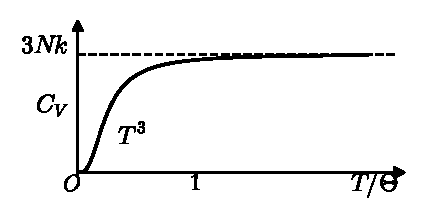
\includegraphics[width=0.72\textwidth]{fig_24.pdf}
\caption*{图 24\quad 比热的 Debye 定律}
\end{figure}

这就是著名的 \emph{Debye 比热公式}。它的结构非常简单。

(i) 当 $T/\Theta$ 大时，积分上限很小，可以把被积函数展开，得到
\begin{equation*}
\int_0^{\Theta/T} \frac{z^4}{z^2}\, dz = \frac{1}{3}\left(\frac{\Theta}{T}\right)^3.
\tag{2.59}
\end{equation*}
于是
\begin{equation*}
C_V = 3Nk,
\tag{2.60}
\end{equation*}
这就是 \emph{Dulong–Petit 定律}。

(ii) 在低温下，积分的上限 $\Theta/T$ 在一切实际场合都可以取作无穷大。这时积分趋于一个常数 $(4\pi^4/15)$，因而
\begin{equation*}
C_V \sim \frac{12\pi^4}{5}\, Nk \left(\frac{T}{\Theta}\right)^3,
\tag{2.61}
\end{equation*}
这就是众所周知的\emph{比热的 $T^3$ 定律}，在低温下成立。

Debye 公式对大多数固体都很有效，Debye 温度已作为固体的一个物理参数被列成表格。它是表征晶格动力学运动的最方便的标度温度：$k\Theta$ 代表在晶格诸模中能够激发的最大量子的能量；$\Theta$ 也应当通过如下关系与晶体中的平均声速相联系：
\begin{equation*}
k\Theta = \hbar q_D\, s.
\tag{2.62}
\end{equation*}

然而，我们在推导这个公式时作了非常粗暴的假设。我们为晶格谱（图 25(a)）假定了一个非常特殊的形式。关系式 $\mathcal{D}(\nu)\propto\nu^2$ 在 $\nu=0$ 附近应当成立，那时材料表现得像一个弹性连续介质，但在
\begin{figure}[H]
\centering
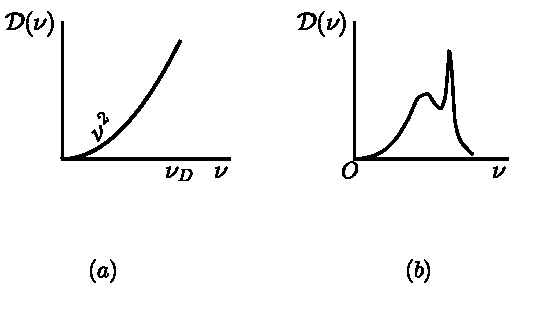
\includegraphics[width=0.72\textwidth]{fig_25.pdf}
\caption*{图 25\quad (a) Debye 谱。(b) 真实的晶格谱}
\end{figure}
$\nu_D$ 处的陡峭截止却并没有根据。精确计算（例如图 25(b)）表明，谱分布在很宽的范围上，带有几个峰，对应于不同偏振的模具有极不相同的速度。高频处往往还有一个相当显著的峰，它源于区边界附近的强色散。$\nu_{\mathbf{q}}$ 随 $\mathbf{q}$ 变化的曲线趋于平坦（参见 §2.2 中的图 22），使得频率相差 $d\nu$ 的诸曲面之间包进了更大的 $\mathbf{q}$ 空间体积。

如果格子是带基元的格子（lattice with a basis），我们还应当计入光学支的贡献。这些模的频率几乎不依赖于波数，因此 \emph{Einstein 模型}（Einstein model）——每个模都具有同一频率——可能更为合适，即
\begin{align*}
C_V &= 3Nk\,\frac{(\hbar\nu_E/kT)^2\, e^{\hbar\nu_E/kT}}{(e^{\hbar\nu_E/kT}-1)^2} \\
&= 3Nk\,\frac{(\Theta_E/T)^2\, e^{\Theta_E/T}}{(e^{\Theta_E/T}-1)^2},
\tag{2.63}
\end{align*}
其中 $\Theta_E$ 是 \emph{Einstein 温度}（Einstein temperature），由下式定义：
\begin{equation*}
k\Theta_E = \hbar\nu_E.
\tag{2.64}
\end{equation*}

然而应当指出，如果把式 (2.57) 中的 $N$ 取作晶体中原子的总数而不是晶胞的数目，我们仍然可以用单独一个 Debye 项来表示复杂晶体的比热。如果我们忽略晶胞内原子彼此之间在位置和质量上的差异，得到的结果正是如此。Debye 公式丝毫不涉及真实的晶体结构，所以这未必是一个坏的近似。实际上，我们正是
利用一个人为扩大的布里渊区——扩展区图式（图 26(a)）——并忽略由此产生的带隙：正如 §2.2 中图 19(c)（原书第 34 页）中那样，这些带隙来自晶胞内各原子之间质量的不同以及动力学相互作用的不同。

\section{晶格谱}

简正模频率分布的实际计算是一个数值计算问题。归根到底，除了对 q 空间中一组密集分布
的 q 值网格求解方程组 (2.13)，再数出有多少个 $\nu_{\mathbf{q}}$ 值落入每个区间
$d\nu$ 之外，别无他法。

但是有一条重要的原理，即 van Hove 定理（van Hove's theorem），它支配着函数
$\mathcal{D}(\nu)$ 及其奇点的性质。这一定理的完整证明超出了本书的范围，但其一般论证
既有意义又重要。

为简单起见，我们考虑谱中的一支。频率落在区间 $d\nu$ 内的模所占的比例等于
\begin{equation*}
\mathcal{D}(\nu)\,d\nu = \frac{v_c}{8\pi^3} \int\!\!\!\int\!\!\!\int d^3 q,
\tag{2.65}
\end{equation*}
其中积分遍及 q 空间中 $\nu \leqslant \nu_{\mathbf{q}} \leqslant \nu + d\nu$
的壳层体积。

我们引入矢量
\begin{equation*}
\mathbf{v}_{\mathbf{q}} \equiv \nabla_{\mathbf{q}}\,\nu_{\mathbf{q}}
\equiv \left( \frac{\partial\nu_q}{\partial q_x},\,
\frac{\partial\nu_q}{\partial q_y},\,
\frac{\partial\nu_q}{\partial q_z} \right),
\tag{2.66}
\end{equation*}
即频率函数在 q 空间中的梯度。这个矢量具有速度的量纲（在 Debye 模型中它就是声速），
并且在所有涉及波的能量传播的问题中都扮演重要角色。事实上，它就是波矢为 $\mathbf{q}$
的波包在晶格这种色散介质中的群速（group velocity）。

我们可以用式 (2.66) 来对式 (2.65) 作一个形式上的简化。令我们在其中积分的 q 空间壳层
内的体积元是一个柱体：其底面是频率面 $\nu_{\mathbf{q}} = \nu$ 上的面元 $dS_\nu$，
高为
\begin{equation*}
dq_\perp = \frac{d\nu}{\left| \partial\nu_{\mathbf{q}}/\partial q \right|}
\tag{2.67}
\end{equation*}
沿曲面法向量出。这个方向正是 $\mathbf{v}_{\mathbf{q}}$ 的方向，于是
\begin{equation*}
\mathcal{D}(\nu)\,d\nu = \frac{1}{8\pi^3 N} \int\!\!\int dS_\nu\, dq_\perp
\tag{2.68}
\end{equation*}

\begin{figure}[H]
\centering
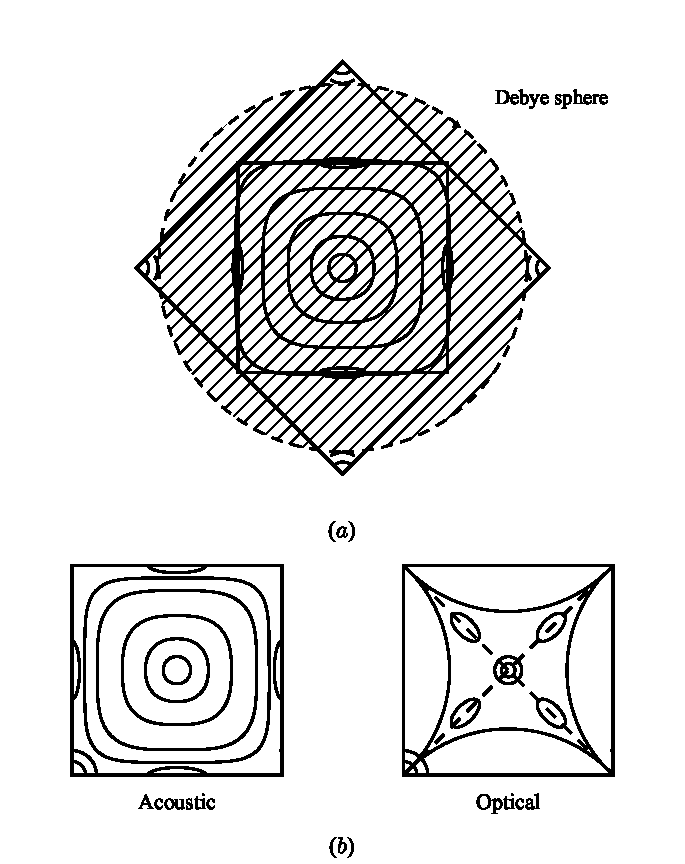
\includegraphics[width=0.72\textwidth]{fig_26.pdf}
\caption*{图 26\quad 声学与光学频率面：(a) 扩展区图式；(b) 分处于两个区中。}
\end{figure}
由此得
\begin{equation*}
\mathcal{D}(\nu) = \frac{1}{8\pi^3 N} \int \frac{dS_\nu}{v_q},
\tag{2.69}
\end{equation*}
其中 $v_q$ 就是矢量 $\mathbf{v}_{\mathbf{q}}$ 的模。

在晶格模谱和电子态谱的理论中我们经常用到这个公式。就其本身而言，它能告诉我们的并不
多，只是关于 $\mathcal{D}(\nu)$ 之奇点的性质。这些奇点必定出现在临界点（critical
point）处，即 $\mathbf{v}_{\mathbf{q}}$ 为零之处，也就是说函数
$\nu_{\mathbf{q}}$ 局部“平坦”之处。

设 $\mathbf{q}_c$ 是一个临界点。由于 $\nu_{\mathbf{q}}$ 是 $\mathbf{q}$
的连续函数，可以在该点附近把它展成 Taylor 级数。线性项因
$\mathbf{v}_{\mathbf{q}} = \mathbf{0}$ 而消失，二次项则可通过主轴变换化为平方和。
于是可以写出
\begin{equation*}
\nu_{\mathbf{q}} = \nu_c + \alpha_1 \xi_1^2 + \alpha_2 \xi_2^2
+ \alpha_3 \xi_3^2 + \ldots,
\tag{2.70}
\end{equation*}
其中 $\boldsymbol{\xi} = \mathbf{q} - \mathbf{q}_c$
是离开临界点的矢距，以局部主轴为参照；系数 $\alpha_1, \alpha_2, \alpha_3$
取决于 $\nu_{\mathbf{q}}$ 对 $\mathbf{q}$ 的局部二阶导数。

例如，设 $\alpha_1, \alpha_2, \alpha_3$ 全为负，则 $\nu$
位于一个局部极大附近。等频面 (2.70) 是椭球面；由初等解析几何可知，
围绕 $\mathbf{q}_c$ 的等值面 $\nu$ 所包围的体积为
\begin{equation*}
\frac{4}{3}\pi\,
\frac{(\nu_c - \nu)^{\frac{3}{2}}}{|\alpha_1 \alpha_2 \alpha_3|^{\frac{1}{2}}},
\tag{2.71}
\end{equation*}
于是由式 (2.65) 出发，对 $\nu$ 求导一次即得
\begin{equation*}
\mathcal{D}(\nu) =
\frac{1}{4\pi^2 N\,|\alpha_1 \alpha_2 \alpha_3|^{\frac{1}{2}}}
(\nu_c - \nu)^{\frac{1}{2}}.
\tag{2.72}
\end{equation*}
此式对 $\nu < \nu_c$ 成立；当 $\nu > \nu_c$ 时，$\mathbf{q}_c$
的邻域对 $\mathcal{D}(\nu)$ 没有贡献。因此，这一奇点并不破坏
$\mathcal{D}(\nu)$ 的连续性，但其斜率 $\partial\mathcal{D}(\nu)/\partial\nu$
不连续，且当 $\nu$ 从下方趋于 $\nu_c$ 时趋于 $-\infty$。

系数 $\alpha_1, \alpha_2, \alpha_3$ 还有其他的可能组合。例如，若一正两负，
我们就得到指标为 1 的鞍点（saddle-point of index 1）。此时，用完全相同的解析几何
方法可以得出，$\nu_c$ 邻域内谱的形状为
\begin{equation*}
\mathcal{D}(\nu) = \left\{
\begin{array}{ll}
C + O(\nu - \nu_c) & (\nu < \nu_c), \\[6pt]
C - \dfrac{1}{4\pi^2 N\,|\alpha_1 \alpha_2 \alpha_3|^{\frac{1}{2}}}
(\nu - \nu_c)^{\frac{1}{2}} + O(\nu - \nu_c) & (\nu > \nu_c),
\end{array}
\right.
\tag{2.73}
\end{equation*}
仍然只是斜率上的一次不连续——一侧带有一条竖直切线——叠加在由区的其他区域产生的光滑
函数 $C + O(\nu - \nu_c)$ 之上。

\begin{figure}[H]
\centering
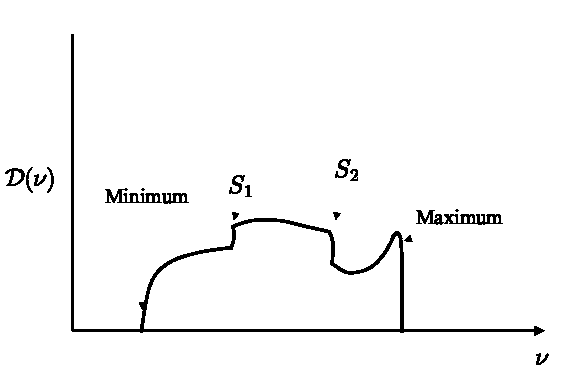
\includegraphics[width=0.72\textwidth]{fig_27.pdf}
\caption*{图 27\quad 不同类型的 van Hove 奇点。}
\end{figure}
事实上，临界点共有四种类型，如图 27 所示，其中 $S_1$ 和 $S_2$
分别指指标为 1 和指标为 2 的鞍点（后者有两个 $\alpha$
为正、一个为负，其表现犹如反过来的式 (2.73)）。极小的情形显然与极大的情形类似。

这些奇点并不十分严重——但却是必不可少的。van Hove 定理实质上断言：\emph{谱必定至少
各含一个 $S_1$ 型与 $S_2$ 型的临界点，且 $\mathcal{D}(\nu)$
的斜率在上端必趋于 $-\infty$}。这一证明需要若干泛函拓扑方面的定理，超出了本书当前的
范围。不过，这一论证可以在二维情形中得到说明（在二维中，鞍点产生对数奇点，而极值点
产生 $\mathcal{D}(\nu)$ 的有限跃变）。

关键在于，函数 $\nu_{\mathbf{q}}$ 是倒格子空间中 $\mathbf{q}$
的连续周期函数。设在区内某点 $m$ 处它有一个极小，则在倒格子的每个对应点处它都有类似
的极小。同样，如果它在区内某点 $M$ 处取极大值，那么这就是一个临界点，对应于重复区图
式中环绕 $M$ 的山丘的峰顶。\footnote{若极大值位于区的角上，我们也许会觉得积分似乎只应
包含落在区内的那一部分。但来自其他角的贡献会自动补足，凑成像式 (2.72)
那样的完整一项。我们也可以通过平移积分区域使之包含一个完整的峰来保证这一点。倒格子的
\emph{任何}一个晶胞都是可取的积分区域；Brillouin 区只不过是约定俗成的选择。}于是，
整个倒格子空间中将有这样一种峰的分布。

现在考虑一条联结两个极大 $M$、$M$ 的路径。函数 $\nu_{\mathbf{q}}$
必定沿这条路径变化；在路径上的某点 $X$ 处，它取得该路径上的极小值。现在让这条路径在
区内移动，就会生成一系列点 $X, X, X$。这些点构成另一条连续路径；由于 $m$ 与 $m$
是 $\nu_{\mathbf{q}}$ 的绝对极小点，这条路径必定经过这些点。

\begin{figure}[H]
\centering
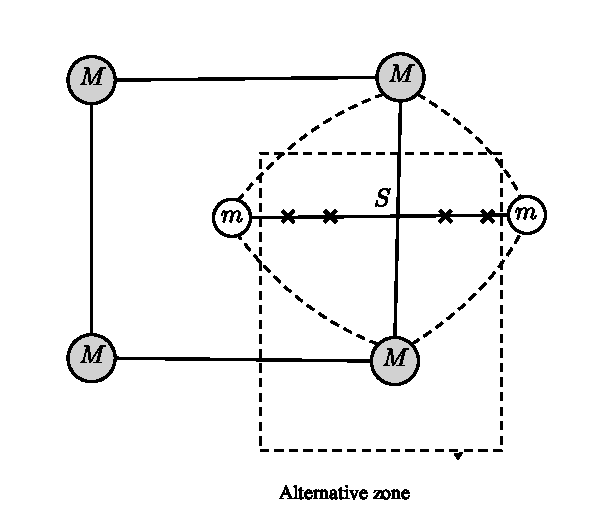
\includegraphics[width=0.72\textwidth]{fig_28.pdf}
\caption*{图 28\quad 寻找鞍点。}
\end{figure}
但现在我们有了一条从两个极小之间穿过的路径 $mm$。在这条路径上必至少有一个极大
$S$。这个点就是一个鞍点——对诸如 $MM$ 的路径而言它是极小，而对诸如 $mm$
的路径而言它是极大。于是，我们的函数 $\nu_{\mathbf{q}}$ 至少有一个 $S$
型的临界点。

在一般的三维问题中，谱有三个声学支，论证更为复杂。区的原点 $\mathbf{q} = 0$
是所有三支的绝对极小——但函数 $\nu_{\mathbf{q}}$ 在该处不能展成 Taylor
级数，而且速度并不为零。横波的两支也不是彼此分立的，因此必须把
$\nu_{\mathbf{q}}$ 当作 $\mathbf{q}$ 的双值函数来处理。不过，上述形式的定理对
总谱仍然成立。当然，实际的临界点可能远多于这个最少数目。

\section{理想晶体的衍射}

如果晶体中的所有原子都严格处在它们“名下”的格点上，那么与晶体相联系的所有可测物理量
都将是严格的周期函数。例如，一个电子的势能将满足条件
\begin{equation*}
\mathcal{V}(\mathbf{r} + \mathbf{l}) = \mathcal{V}(\mathbf{r}).
\tag{2.74}
\end{equation*}

设有一束快速电子射入晶体。由于被这个势散射，电子将从一个电子态跃迁到另一个电子态。
在微扰论的 Born 近似中，初态 $\Psi_{\mathbf{k}}$ 与末态 $\Psi_{\mathbf{k}'}$
之间的跃迁速率正比于矩阵元
\begin{equation*}
\mathcal{M}_{\mathbf{k}'\mathbf{k}} \equiv \int \Psi_{\mathbf{k}'}^{*}(\mathbf{r})\,
\mathcal{V}(\mathbf{r})\, \Psi_{\mathbf{k}}(\mathbf{r})\, \mathrm{d}\mathbf{r}.
\tag{2.75}
\end{equation*}
的平方。

我们取这些态为平面波态
\begin{equation*}
\Psi_{\mathbf{k}} = e^{i\mathbf{k}\cdot\mathbf{r}}.
\tag{2.76}
\end{equation*}
我们又由式 (1.15) 知道，势可以展成 Fourier 级数
\begin{equation*}
\mathcal{V}(\mathbf{r}) = \sum_{\mathbf{g}} \mathcal{V}_{\mathbf{g}}\,
e^{i\mathbf{g}\cdot\mathbf{r}}.
\tag{2.77}
\end{equation*}
于是
\begin{align*}
\mathcal{M}_{\mathbf{k}'\mathbf{k}}
&= \int e^{-i\mathbf{k}'\cdot\mathbf{r}} \sum_{\mathbf{g}}
\mathcal{V}_{\mathbf{g}}\, e^{i\mathbf{g}\cdot\mathbf{r}}\,
e^{i\mathbf{k}\cdot\mathbf{r}}\, \mathrm{d}\mathbf{r} \\
&= \sum_{\mathbf{g}} \mathcal{V}_{\mathbf{g}} \int
e^{i(\mathbf{k}+\mathbf{g}-\mathbf{k}')\cdot\mathbf{r}}\, \mathrm{d}\mathbf{r} \\
&= \left\{ \begin{array}{ll}
\mathcal{V}_{\mathbf{g}} & \text{若}\quad \mathbf{k}+\mathbf{g}-\mathbf{k}' = 0, \\
0 & \text{其余情形}. \\
\end{array} \right\}
\tag{2.78}
\end{align*}

如果 $\mathbf{k}$ 是固定的——也就是说，入射电子束是单色的且方向高度确定——那么我们
只能在满足
\begin{equation*}
\mathbf{k}' = \mathbf{k} + \mathbf{g},
\tag{2.79}
\end{equation*}
的方向上观察到衍射束，其中 $\mathbf{g}$
是晶体的倒格矢之一。

在这种情形下我们还必须坚持：衍射束的能量与入射能量相同，即两个波矢长度相等。这就给
散射角加上了一个条件。若 $2\theta$ 是 $\mathbf{k}$ 与 $\mathbf{k}'$
之间的夹角，则
\begin{equation*}
|\mathbf{g}| = 2|\mathbf{k}|\sin\theta.
\tag{2.80}
\end{equation*}
为了在倒格子空间中满足这些几何条件，我们作出 \emph{Ewald 球}（Ewald
sphere）（图 29(b)），其半径 $OP$ 等于入射波矢。若把倒格子的原点放在 $P$，则矢量
$\mathbf{g}$ 必定把我们带到 $Q$ 点，$OQ$ 即波矢 $\mathbf{k}'$。因此，只要晶体
相对于入射束的取向恰好使倒格子的一个格点落在球面上，就会发生衍射。

\begin{figure}[H]
\centering
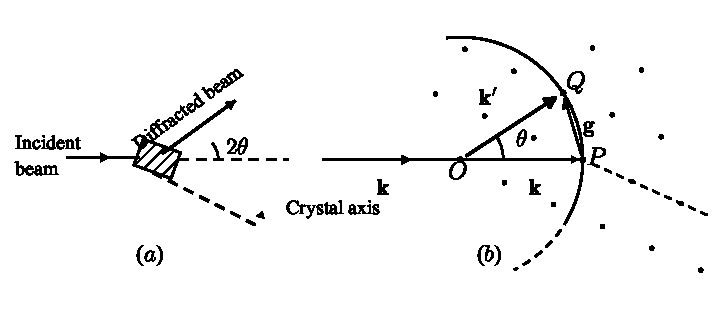
\includegraphics[width=0.72\textwidth]{fig_29.pdf}
\caption*{图 29\quad (a) X 射线衍射；(b) Ewald 作图法。}
\end{figure}
我们可以换一种方式来表述这一点。正如 §1.3 中所指出的，倒格矢的长度正比于它所垂直的
晶面族的面间距 $d$ 的倒数，即
\begin{equation*}
|\mathbf{g}| = \frac{2\pi n}{d},
\tag{2.81}
\end{equation*}
其中 $n$ 是整数（$\mathbf{g}$ 在倒格子三矢组（reciprocal triad）
各轴上分量的最大公约数）。于是，若 $\lambda$ 是入射电子的波长，则式 (2.80) 与
(2.81) 给出
\begin{equation*}
n\lambda = 2d\sin\theta.
\tag{2.82}
\end{equation*}
这就是所谓的 \emph{Bragg 反射定律}（Bragg reflection law）。它很容易通过考察从相继
各晶面上反射的束之间的相位关系推出：要发生相干衍射，附加路径 $ABC$
必须是波长的整数倍（图 30）。

散射矩阵元的大小取决于 $\mathcal{V}_{\mathbf{g}}$。对电子而言，这似乎就是局域势的
各 Fourier 分量——但当我们处理极慢电子时这种看法会导致误解，我们将在 §3.6
再回到这一点。同样的理论也适用于 X 射线的衍射，只是 X 射线响应的是晶体中的局域电子
密度。由于电子密度同样是一个像 (2.74) 那样的周期函数，衍射图样在定性上是相同的。本节
的理论自然进而引出 X 射线晶体结构分析那令人赞叹的复杂性与种种成就。

在中子的情形，散射主要来自原子核：它在空间中的行为像一个 $\delta$
函数型的势，而且随元素不同而有相当大的变化。事实上，由于同一元素的不同同位素可能具有
差别很大的中子
散射截面，并且在晶体中随机混在一起，所以总会有一些\emph{非相干}（incoherent）
散射，它给衍射图样添上一片弥漫的背景。即使晶体中只存在一种同位素，这种情形也可能发生，
因为中子对原子核的自旋取向是敏感的。

\begin{figure}[H]
\centering
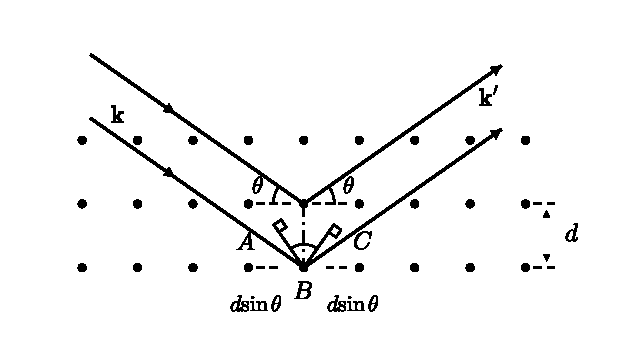
\includegraphics[width=0.72\textwidth]{fig_30.pdf}
\caption*{图 30\quad Bragg 衍射。}
\end{figure}
\begin{figure}[H]
\centering
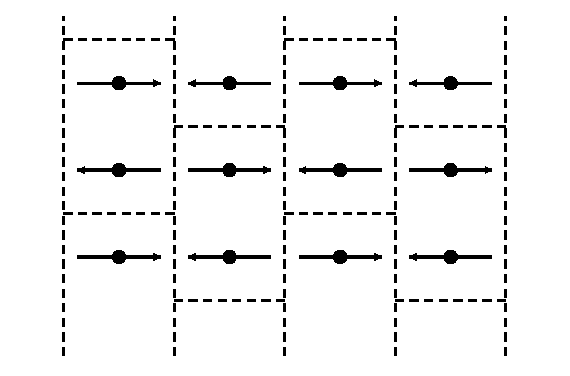
\includegraphics[width=0.72\textwidth]{fig_31.pdf}
\caption*{图 31\quad 反铁磁排列，显示出加倍了的晶胞。}
\end{figure}
中子衍射在分析\emph{反铁磁}（antiferromagnetic）晶体时特别有用。在这类晶体中，原子
具有永久原子磁矩，它们以如下方式极化并排列：一个子晶格上的所有原子磁矩指向一个方向，
另一子晶格上的所有原子磁矩指向相反的方向。我们将在 §§10.6、10.11
中讨论这种系统的磁性质。

这里我们只指出：中子带有磁矩，对每个原子处的局域磁场敏感，因而能够区分磁矩取向不同的
原子。其结果是结构的周期单元变大了，这意味着有效布里渊区的尺寸变小了。新的倒格矢被
引入（可对照图 19），于是衍射图样中出现了新的线，称为磁超格线（magnetic
superlattice lines）。

晶体衍射的这一初等\emph{几何理论}（geometrical
theory）忽略了若干实际上的复杂因素，例如下一节要讨论的热振动的效应。我们还必须考虑
入射束与衍射束在穿过较厚样品时与一层层原子持续相互作用的问题。由此产生若干复杂的效应，
例如\emph{初级消光}（primary extinction）和\emph{摆动效应}（pendulum
effect，即“Pendellösung”），对它们的解释要用到 X 射线衍射的\emph{动力学理论}
（dynamical theory）。其要点是：X
射线（或电子、或中子）在晶体中传播时经受速度色散，在接近相干衍射条件时尤其如此（参见
§3.3）。处在不同色散面上的两束或更多的束可以同时被激发，并在穿过样品时相互干涉。在
\emph{低能电子衍射}（low energy electron diffraction，L.E.E.D.）
的情形，这类效应完全支配着实验现象（参见 §6.9）。

\section{含晶格振动的晶体衍射}

现在考虑更一般的情形：势未必是周期的。设它是各个原子势叠加的结果：
\begin{equation*}
\mathcal{V}(\mathbf{r}) = \sum_{\boldsymbol{l}} \mathcal{V}_a(\mathbf{r} - \mathbf{R}_{\boldsymbol{l}}),
\tag{2.83}
\end{equation*}
其中 $\mathbf{R}_{\boldsymbol{l}}$
是本应处在格点 $\boldsymbol{l}$ 上的那个原子（或离子）的实际位置，而
$\mathcal{V}_a$ 是单个原子的势场。为记号简单起见，我们假定是 Bravais 格子。

于是我们可以像式 (2.75) 那样，计算从态 $\Psi_{\mathbf{k}}$ 散射到态
$\Psi_{\mathbf{k}'}$ 的矩阵元：
\begin{align*}
\mathcal{M}_{\mathbf{k}'\mathbf{k}}
&= \int e^{-i\mathbf{k}'\cdot\mathbf{r}} \sum_{\boldsymbol{l}}
\mathcal{V}_a(\mathbf{r} - \mathbf{R}_{\boldsymbol{l}})\,
e^{i\mathbf{k}\cdot\mathbf{r}}\, \mathrm{d}\mathbf{r} \\
&= \sum_{\boldsymbol{l}} \int e^{i(\mathbf{k}-\mathbf{k}')\cdot\mathbf{r}}\,
\mathcal{V}_a(\mathbf{r} - \mathbf{R}_{\boldsymbol{l}})\, \mathrm{d}\mathbf{r} \\
&= \sum_{\boldsymbol{l}} e^{i(\mathbf{k}-\mathbf{k}')\cdot\mathbf{R}_{\boldsymbol{l}}}
\int e^{i(\mathbf{k}-\mathbf{k}')\cdot(\mathbf{r}-\mathbf{R}_{\boldsymbol{l}})}
\mathcal{V}_a(\mathbf{r} - \mathbf{R}_{\boldsymbol{l}})\, \mathrm{d}\mathbf{r}.
\tag{2.84}
\end{align*}

求和中的每个积分名义上遍及整个空间——至少遍及整个晶体。但我们预计原子势
$\mathcal{V}_a(\mathbf{r})$ 的作用范围非常有限，所以积分结果几乎不会依赖于计量它所
用的中心 $\mathbf{R}_{\boldsymbol{l}}$。我们引入\emph{散射矢量}（scattering vector）
\begin{equation*}
\mathbf{K} = \mathbf{k}' - \mathbf{k};
\tag{2.85}
\end{equation*}
于是矩阵元变为
\begin{equation*}
\mathcal{M}_{\mathbf{k}'\mathbf{k}} = \mathcal{V}_a(\mathbf{K}) \cdot
\frac{1}{N} \sum_{\boldsymbol{l}} e^{-i\mathbf{K}\cdot\mathbf{R}_{\boldsymbol{l}}},
\tag{2.86}
\end{equation*}
其中我们把原子势的 Fourier 变换定义为\footnote{我们引入 $N = 1/v_c$
——宏观单位体积晶体中的晶胞数——以使 $\mathcal{V}_a(\mathbf{K})$
具有能量的量纲。式 (2.84) 中用到的平面波态 (2.76)
显然也是按这个宏观单位体积归一化的。}
\begin{equation*}
\mathcal{V}_a(\mathbf{K}) \equiv \frac{1}{v_c} \int
\mathcal{V}_a(\mathbf{r})\, e^{-i\mathbf{K}\cdot\mathbf{r}}\, \mathrm{d}\mathbf{r}.
\tag{2.87}
\end{equation*}

把式 (2.86) 分解成一个\emph{原子因子}（atomic factor）和一个\emph{结构因子}
（structure factor）是极为有用的。我们先考虑理想晶格的结构因子，即令
\begin{equation*}
\mathbf{R}_{\boldsymbol{l}} = \boldsymbol{l}
= l_1\mathbf{a}_1 + l_2\mathbf{a}_2 + l_3\mathbf{a}_3
\tag{2.88}
\end{equation*}
对所有格点都成立。

把散射矢量写成
\begin{equation*}
\mathbf{K} = K_1\mathbf{b}_1 + K_2\mathbf{b}_2 + K_3\mathbf{b}_3,
\tag{2.89}
\end{equation*}
其中 $\mathbf{b}_1, \mathbf{b}_2, \mathbf{b}_3$
是倒格子三矢组 (1.19)。于是结构因子变为
\begin{align*}
\sum_{\boldsymbol{l}} e^{-i\mathbf{K}\cdot\boldsymbol{l}}
&= \sum_{l_1,l_2,l_3} e^{-i(K_1 l_1 + K_2 l_2 + K_3 l_3)} \\
&= \Bigl( \sum_{0 \leqslant l_1 < L_1} e^{-iK_1 l_1} \Bigr)
   \Bigl( \sum_{0 \leqslant l_2 < L_2} e^{-iK_2 l_2} \Bigr)
   \Bigl( \sum_{0 \leqslant l_3 < L_3} e^{-iK_3 l_3} \Bigr) \\
&= \left( \frac{1 - e^{-iK_1 L_1}}{1 - e^{-iK_1}} \right)
   \left( \frac{1 - e^{-iK_2 L_2}}{1 - e^{-iK_2}} \right)
   \left( \frac{1 - e^{-iK_3 L_3}}{1 - e^{-iK_3}} \right),
\tag{2.90}
\end{align*}
其中，如同式 (1.76) 中那样，$L_1, L_2, L_3$
是沿晶体块体各边的晶胞数。

式 (2.90) 中的每个因子只是 1 的量级，并且随 $\mathbf{K}$ 的变化剧烈起伏。对
$\mathbf{K}$ 的一段取值区间作任何平均都会给出零——除非平均区间包含了所有分母的零点，
即
\begin{equation*}
e^{-iK_1} = e^{-iK_2} = e^{-iK_3} = 1,
\tag{2.91}
\end{equation*}
这只有在 $K_1, K_2, K_3$ 各自都是 $2\pi$
的整数倍时才成立。但根据式 (1.20)，这正是 $\mathbf{K}$
应与倒格矢之一重合的条件。

当 $\mathbf{K}$ 真的等于某个倒格矢时，式 (2.90)
中每一项的分子和分母都变为零。不过这时我们回到原来的求和式，注意到每一项都具有
$\exp(-i\mathbf{g}\cdot\boldsymbol{l})$ 的形式，恰好等于 1，于是求和正好是
$N$。这样我们就得到重要的规则
\begin{equation*}
\frac{1}{N} \sum_{\boldsymbol{l}} e^{-i\mathbf{K}\cdot\boldsymbol{l}}
= \delta_{\mathbf{K}\,\mathbf{g}},
\tag{2.92}
\end{equation*}
其中 $\delta$ 记号在 $\mathbf{K}$ 不是集合 $\{\mathbf{g}\}$
中的矢量时为零。

把式 (2.92) 代回式 (2.86)，便得
\begin{equation*}
\mathcal{M}_{\mathbf{k}'\mathbf{k}}
= \mathcal{V}_a(\mathbf{g})\, \delta_{\mathbf{k}'-\mathbf{k},\,\mathbf{g}},
\tag{2.93}
\end{equation*}
这正是我们先前的结果 (2.78)。

但现在假设晶体的晶格模被激发了。每个原子都偏离其理想格点：
\begin{align*}
\mathbf{R}_{\boldsymbol{l}} &= \boldsymbol{l} + \mathbf{u}_{\boldsymbol{l}} \\
&= \boldsymbol{l} + \sum_{\mathbf{q}>}
\left( \mathbf{U}_{\mathbf{q}}\, e^{i\mathbf{q}\cdot\boldsymbol{l}}
+ \mathbf{U}_{\mathbf{q}}^{*}\, e^{-i\mathbf{q}\cdot\boldsymbol{l}} \right),
\tag{2.94}
\end{align*}
其中 $\mathbf{U}_{\mathbf{q}}$ 如式 (2.8) 与 (2.10)
中那样，是波矢为 $\mathbf{q}$ 的模的矢量振幅。求和只遍及 $\mathbf{q}$
取值范围的一半，这样我们就可以把复共轭项 $\mathbf{U}_{\mathbf{q}}^{*} =
\mathbf{U}_{-\mathbf{q}}$ 明写出来，使位移为实。

把式 (2.94) 代入式 (2.86) 的结构因子中：
\begin{align*}
\frac{1}{N} \sum_{\boldsymbol{l}} e^{-i\mathbf{K}\cdot\mathbf{R}_{\boldsymbol{l}}}
&= \frac{1}{N} \sum_{\boldsymbol{l}} \exp\bigl[ -i\mathbf{K}\cdot
\bigl\{ \boldsymbol{l} + \sum_{\mathbf{q}>}
(\mathbf{U}_{\mathbf{q}}\, e^{i\mathbf{q}\cdot\boldsymbol{l}}
+ \mathbf{U}_{\mathbf{q}}^{*}\, e^{-i\mathbf{q}\cdot\boldsymbol{l}}) \bigr\} \bigr] \\
&= \frac{1}{N} \sum_{\boldsymbol{l}} \bigl[ e^{-i\mathbf{K}\cdot\boldsymbol{l}}
\prod_{\mathbf{q}>} \exp\bigl\{ -i\mathbf{K}\cdot
(\mathbf{U}_{\mathbf{q}}\, e^{i\mathbf{q}\cdot\boldsymbol{l}}
+ \mathbf{U}_{\mathbf{q}}^{*}\, e^{-i\mathbf{q}\cdot\boldsymbol{l}}) \bigr\}
\bigr].
\tag{2.95}
\end{align*}

这是严格的。让我们把宗量正比于 $\mathbf{U}_{\mathbf{q}}$
的那个指数函数展开——假定它是小位移：
\begin{align*}
&\exp \bigl\{ -i\mathbf{K}\cdot
(\mathbf{U}_{\mathbf{q}}\, e^{i\mathbf{q}\cdot\boldsymbol{l}}
+ \mathbf{U}_{\mathbf{q}}^{*}\, e^{-i\mathbf{q}\cdot\boldsymbol{l}}) \bigr\} \\
&\qquad = 1 - i\mathbf{K}\cdot
(\mathbf{U}_{\mathbf{q}}\, e^{i\mathbf{q}\cdot\boldsymbol{l}}
+ \mathbf{U}_{\mathbf{q}}^{*}\, e^{-i\mathbf{q}\cdot\boldsymbol{l}})
- |\mathbf{K}\cdot\mathbf{U}_{\mathbf{q}}|^2 \ldots
\tag{2.96}
\end{align*}

代入式 (2.95) 后显然可见，把乘积展开时，会出现一个形如 (2.90)
的项，给出理想晶体结构的衍射图样；
其后是所有与 $\mathbf{K}\cdot\mathbf{U}_{\mathbf{q}}$
呈线性关系的项之和，即形如
\begin{align*}
\frac{1}{N} \sum_{\boldsymbol{l}} e^{-i\mathbf{K}\cdot\boldsymbol{l}}
\sum_{\mathbf{q}} \left( -i\mathbf{K}\cdot\mathbf{U}_{\mathbf{q}} \right)
e^{i\mathbf{q}\cdot\boldsymbol{l}}
&= \frac{1}{N} \sum_{\mathbf{q}} \left( -i\mathbf{K}\cdot\mathbf{U}_{\mathbf{q}} \right)
\sum_{\boldsymbol{l}} e^{i(\mathbf{q}-\mathbf{K})\cdot\boldsymbol{l}} \\
&= \sum_{\mathbf{q}} \left( -i\mathbf{K}\cdot\mathbf{U}_{\mathbf{q}} \right)
\delta_{\mathbf{K}-\mathbf{q},\,\mathbf{g}}
\tag{2.97}
\end{align*}
的项——最后一步用了式 (2.92)。正如我们将在 §2.9
中看到的，式 (2.96) 中的模平方项也很重要，因为它的符号不变。

为了理解这一结果，让我们考虑两种情形。在图 32(a) 中，$\mathbf{K}$
位于布里渊区之内。也就是说，我们在这样的态的区域中寻找被散射的电子（或 X
射线、中子）：其中 $\mathbf{k}'$ 与初态 $\mathbf{k}$ 相差不超过半个倒格矢。按惯例，波矢
$\mathbf{q}$ 被限制在一个布里渊区内，于是式 (2.97)
中剩下的唯一一项就是 $\mathbf{q} = \mathbf{K}$ 的那一项。换言之，这一跃迁的矩阵元为
\begin{equation*}
\mathcal{M}_{\mathbf{k}'\mathbf{k}} = -i\{(\mathbf{k}'-\mathbf{k})\cdot
\mathbf{U}_{\mathbf{q}}\}\, \mathcal{V}_a(\mathbf{k}'-\mathbf{k}),
\tag{2.98}
\end{equation*}
其中
\begin{equation*}
\mathbf{q} = \mathbf{k}' - \mathbf{k}.
\tag{2.99}
\end{equation*}

\begin{figure}[H]
\centering
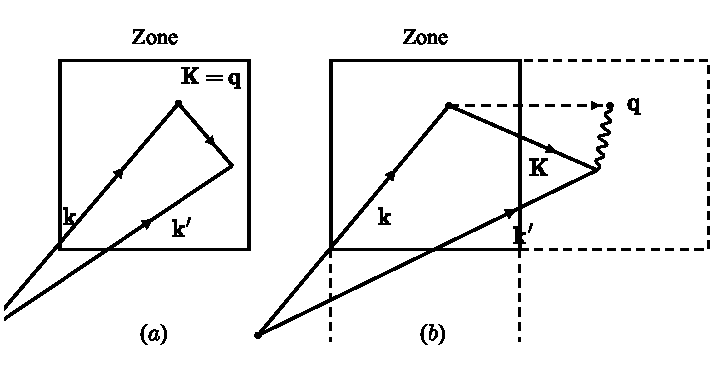
\includegraphics[width=0.72\textwidth]{fig_32.pdf}
\caption*{图 32\quad (a) 正常过程；(b) 倒逆过程（Umklapp 过程）。}
\end{figure}

如果 $\mathbf{K}$ 并\emph{不}落在第一布里渊区内（图 32(b)），式 (2.97)
的求和式中仍然会剩下一项。也就是说，仍然存在一个 $\mathbf{q}$
值满足 $\mathbf{K} - \mathbf{q} = \mathbf{g}$，即满足
\begin{equation*}
\mathbf{q} = \mathbf{k}' - \mathbf{k} - \mathbf{g}.
\tag{2.100}
\end{equation*}

布里渊区作为倒格子的一个晶胞，可以重复铺排而恰好盖满矢量 $\mathbf{K}$ 的整个空间；$\mathbf{K}$ 的任何一个值都可以唯一地由一个 $\mathbf{g}$ 值——倒格子的一个平移矢——和一个 $\mathbf{q}$ 值构造出来，$\mathbf{q}$ 是一个被限制在该格子一个晶胞之内的矢量。用 §1.5 的语言来说，$\mathbf{q}$ 就是 $\mathbf{K}$ \emph{约化}（reduced）到第一布里渊区后的值。

因此，在这两种情形下式 (2.98) 都成立，其中 $\mathbf{q}$ 由 (2.99) 或 (2.100) 给出，视何者适用而定；如果我们把 $\mathbf{g}=0$ 也包括进倒格矢的完全集合之中，则关系式 (2.100) 恒成立。无论我们选取哪个方向，总会有一些散射，只不过其振幅将取决于碰巧具有满足这些条件的正确波矢的那些晶格振动的振幅。

\section{声子}

一个散射过程能否发生，并不单由矩阵元异于零所决定；还有能量条件需要满足。在理想晶格的情形，整个系统是静态的，因此初态和末态的电子（X 射线、中子）具有相同的能量。

的确，晶格处于不断的运动之中。(2.94) 中的矢量 $\mathbf{U}_{\mathbf{q}}$ 应当含有形如 $\exp(i\nu_{\mathbf{q}}t)$ 的时间因子，其中 $\nu_{\mathbf{q}}$ 是波矢为 $\mathbf{q}$ 的简正模的频率。实际上，$\mathbf{U}_{\mathbf{q}}$ 是三个这类矢量之和，它们的振幅、方向和频率各不相同，对应于该波矢的三个不同的声学模。但我们一次只取其中一个，并且记住，入射束与散射束的态 $\Psi_{\mathbf{k}}$ 和 $\Psi_{\mathbf{k}'}$ 必须具有能量 $\mathcal{E}(\mathbf{k})$ 和 $\mathcal{E}(\mathbf{k}')$，从而带有形如 $\exp\{i\mathcal{E}(\mathbf{k})t/\hbar\}$ 与 $\exp\{i\mathcal{E}(\mathbf{k}')t/\hbar\}$ 的时间因子。当我们对时间求平均时，将会遇到如下形式的积分
\begin{equation*}
\int \exp[i\{\mathcal{E}(\mathbf{k})-\mathcal{E}(\mathbf{k}')+\hbar\nu_{\mathbf{q}}\}t/\hbar]\,dt,
\end{equation*}
除非
\begin{equation*}
\mathcal{E}(\mathbf{k})-\mathcal{E}(\mathbf{k}')+\hbar\nu_{\mathbf{q}}=0.
\tag{2.101}
\end{equation*}
否则它们恒为零。换言之，衍射是\emph{非弹性}的；束流获得了与之相互作用的那个晶格模的一个能量量子。

其实这还不完全，因为晶格振动中还会出现共轭的时间依赖 $\exp(-i\nu_{\mathbf{q}}t)$，从而给出电子损失能量 $\hbar\nu_{\mathbf{q}}$ 的衍射。在这两种情形下，我们上面勾画的论证都可以借助于标准的时间依赖微扰理论而变得完全严格。

条件 (2.100) 与 (2.101) 可以给出一种非常直观的解释。我们说，入射电子（或 X 射线、中子）与晶格相互作用而消灭（或产生）了一个\emph{声子}（phonon），其波矢为 $\mathbf{q}$，能量为 $\hbar\nu_{\mathbf{q}}$。我们用图 33$(a)$ 或 $(b)$ 那样的图形来表示这些过程。条件 (2.101) 就是该过程中的能量守恒规则。

如果我们考察对第一区中 $(\mathbf{k}'-\mathbf{k})$ 的一切值都成立的条件 (2.99)，就会发现它看上去像一条动量守恒定律。乘以 $\hbar$，便得
\begin{equation*}
\hbar\mathbf{k}'=\hbar\mathbf{k}+\hbar\mathbf{q}.
\tag{2.102}
\end{equation*}
电子的动量吸收了被消灭的那个声子的\emph{晶体动量}（crystal momentum）$\hbar\mathbf{q}$。这正是为“声子”这个名称辩护的论证——声子是一种具有“类粒子”性质的量子化声激发，与“光子”相类比。

\begin{figure}[H]
\centering
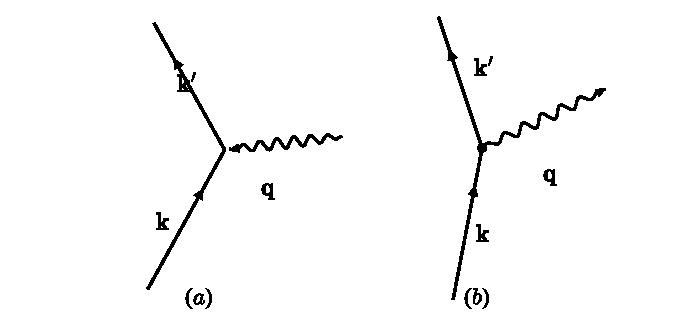
\includegraphics[width=0.72\textwidth]{fig_33.pdf}
\caption*{图 33\quad 电子散射过程：(a) 声子吸收；(b) 声子发射。}
\end{figure}

但在一般情形下，这条“动量守恒规则”并不成立；正如 (2.100) 所表明的，除声子的动量之外，电子还可以获得或失去动量 $\hbar\mathbf{g}$。我们称这样的过程为倒逆过程（Umklapp process），或 U 过程（U-process）。特殊情形 (2.102) 则可称为正常过程（Normal process），或 N 过程（N-process）。

这个结果其实并不令人惊讶。额外的动量 $\hbar\mathbf{g}$ 只不过是传给了作为整体的晶体。在构造晶格振动态时，我们忽略了理想晶格质心的运动——晶格振动正是相对于它来度量的。可以查验，只要把与这个自由度相联系的运动包括进来，基本的动量守恒定律总体上仍然得到满足。一个倒逆过程可以看成是在产生（或消灭）一个声子的同时发生了一次 Bragg 反射；后一过程中的动量显然传给了作为整体的晶体。

非弹性衍射现象是研究晶体晶格动力学的一种极有价值的工具。沿特定方向衍射的束流与具有确定波矢 $\mathbf{q}$ 的晶格模相联系。我们可以考察衍射粒子能量的变化，从而测出 $\hbar\nu_{\mathbf{q}}$。通过朝不同方向观察，并把晶体转到不同的取向，就可以把整个函数 $\nu_{\mathbf{q}}$ 测绘出来。当然，它有若干个不同偏振的分支，但通过系统分析可以把它们分开。中子对局部磁矩的敏感性（§2.6）意味着，对极化中子束被磁振子（magnons）非弹性衍射的情形也有一个类似的理论（见 §10.10），从而给出关于磁振子色散性质的类似信息。

然而，这个实验只有用“热”中子才切实可行；这种中子在能量约为 0.1 eV 时，其波长与晶格间距同数量级。由声子能量引起的频移——其数量级为 $k\Theta$ 或更小，也许 0.01 eV——很容易观察到。对于电子和 X 射线，束流的能量必须高得多——几十或几百电子伏——因此衍射过程中微小的能量变化无法被探测到。

晶体动量的选择定则 (2.102) 依赖于晶格的长程序。当这种有序不存在时，比如在液体或玻璃中，我们会观察到什么？弹性衍射将依赖于矩阵元 (2.86) 的平方，后者正比于结构因子的平方：
\begin{align*}
S(\mathbf{K}) &\equiv \left|\frac{1}{N}\sum_{\mathbf{l}} e^{-i\mathbf{K}\cdot\mathbf{R}_{\mathbf{l}}}\right|^{2}\\
&= \frac{1}{N^{2}}\sum_{\mathbf{l}\mathbf{l}'} e^{-i\mathbf{K}\cdot(\mathbf{R}_{\mathbf{l}}-\mathbf{R}_{\mathbf{l}'})}\\
&= \frac{1}{N}\int P(\mathbf{R})\,e^{-i\mathbf{K}\cdot\mathbf{R}}\,\mathrm{d}\mathbf{R}.
\tag{2.103}
\end{align*}
衍射图样依赖于对关联函数（pair correlation function）$P(\mathbf{R})$——即在相距 $\mathbf{R}$ 处找到两个原子的概率——的 Fourier 变换。在液体中，这正是我们熟悉的体系的径向分布函数（radial distribution function）。

对这个论证作一个简单的推广即可证明，非弹性衍射的振幅 $S(\mathbf{K},\nu)$ 必定是含时关联函数（time-dependent correlation function）$P(\mathbf{R},t)$ 的双重 Fourier 变换，$P(\mathbf{R},t)$ 度量的是这样的概率：已知在时刻 0 有一个原子（可能就是同一个）位于原点 0，在时刻 $t$ 于点 $\mathbf{R}$ 处找到一个原子的概率。例如，中子衍射可以测量波矢为 $\mathbf{K}$ 的密度涨落的频谱——这个物理量恰好只有在相当完善的晶格中才相当尖锐。类似地，极化中子会被自旋密度（spin density）涨落所衍射，这些涨落由类似的关联函数或它们在空间或动量、时间或能量上的 Fourier 变换所定义。

\section{德拜–沃勒因子}

(2.97) 中那些对应于含一个声子的散射过程的项，并不是结构因子 (2.95) 中可能出现的一切。容易看出，类似 (2.96) 的那些因子的乘积，以及指数展开中更高阶的项，会产生包含形如 $\mathbf{U}_{\mathbf{q}}\exp(i\mathbf{q}\cdot\mathbf{l})$ 的因子的各种乘积的贡献。对每一个这样的因子，我们都称相应的声子被产生或消灭了，因此这些项属于多声子过程（multiphonon processes）。

总的来说，随着阶数升高，这些过程的速率迅速下降，对非弹性衍射背景的贡献并不很大。然而，有一类重要的项来自展开式 (2.96) 中的平方项 $-|\mathbf{K}\cdot\mathbf{U}_{\mathbf{q}}|^{2}$，它们平均之后并不给出小的贡献。考察 (2.95) 与 (2.96) 即可发现，无论是弹性还是非弹性散射，矩阵元的平方都应当乘以
\begin{equation*}
e^{-2W}=\prod_{\mathbf{q}}\left\{1-|\mathbf{K}\cdot\mathbf{U}_{\mathbf{q}}|^{2}\right\},
\tag{2.104}
\end{equation*}
现在 $\mathbf{q}$ 则重新取遍整个布里渊区。

这个量称为 Debye–Waller 因子（Debye–Waller factor）。把它写成这种形式，是因为我们可以利用一条标准的代数定理
\begin{equation*}
\lim_{N\to\infty}\prod_{n=1}^{N}\left(1-\frac{1}{N}a_{n}\right)=\exp\left\{-\lim_{N\to\infty}\frac{1}{N}\sum_{n=1}^{N}a_{n}\right\},
\tag{2.105}
\end{equation*}
把乘积变换成求和。于是
\begin{equation*}
e^{-2W}=\exp\left\{-\sum_{\mathbf{q}}\frac{1}{2}\,|\mathbf{K}\cdot\mathbf{U}_{\mathbf{q}}|^{2}\right\},
\tag{2.106}
\end{equation*}
即
\begin{equation*}
W=\frac{1}{2}\sum_{\mathbf{q}}|\mathbf{K}\cdot\mathbf{U}_{\mathbf{q}}|^{2}.
\tag{2.107}
\end{equation*}
要计算这个和，我们需要知道第 $\mathbf{q}$ 个晶格模的振幅 $\mathbf{U}_{\mathbf{q}}$。它将是温度的函数。我们知道，该模中的平均能量由 (2.47) 给出：
\begin{equation*}
\bar{\mathcal{E}}_{\mathbf{q}}=\left(\bar{n}_{\mathbf{q}}+\frac{1}{2}\right)\hbar\nu_{\mathbf{q}},
\end{equation*}
其中 $\bar{n}_{\mathbf{q}}$ 是该模中声子的平均数，由 Bose–Einstein 公式 (2.46) 给出。

在经典处理中，我们可以把每个简谐振子模的能量算成其动能与势能之和。众所周知，这两者相等——于是由 (2.1) 和 (2.8) 得
\begin{align*}
\bar{\mathcal{E}}&=\sum_{s\mathbf{l}}M_{s}\,|\dot{\mathbf{u}}_{s\mathbf{l}}|^{2}\\
&=\sum_{s\mathbf{q}}NM_{s}\,|\dot{\mathbf{U}}_{s\mathbf{q}}|^{2}\\
&=\sum_{s\mathbf{q}}NM_{s}\,\nu_{\mathbf{q}}^{2}|\mathbf{U}_{s\mathbf{q}}|^{2}.
\tag{2.108}
\end{align*}
如果每个晶胞只有一个原子，质量为 $M$，则
\begin{align*}
|\mathbf{U}_{\mathbf{q}}|^{2}&=\bar{\mathcal{E}}_{\mathbf{q}}/NM\nu_{\mathbf{q}}^{2}\\
&=(\bar{n}_{\mathbf{q}}+\tfrac{1}{2})\hbar/NM\nu_{\mathbf{q}}.
\tag{2.109}
\end{align*}
我们知道 $\mathbf{U}_{\mathbf{q}}$ 在晶格谱每一支上的偏振，所以原则上能够精确计算出 Debye–Waller 因子。

为了看出它应当有怎样的行为，让我们假定一个三个模都具有相同速度的 Debye 模型。对任一偏振，平均而言我们应得
\begin{equation*}
|\mathbf{K}\cdot\mathbf{U}_{\mathbf{q}}|^{2}=\tfrac{1}{3}K^{2}|\mathbf{U}_{\mathbf{q}}|^{2},
\tag{2.110}
\end{equation*}
但若计入三个不同的偏振，因子 $\frac{1}{3}$ 便消去了。\footnote{有一条有用的规则：在这个模型中，三个模对每个 $\mathbf{q}$ 值都是简并的。因此可以随意选取偏振矢量，只要它们相互正交。于是可以取一个模的 $\mathbf{U}_{\mathbf{q}}$ 平行于 $\mathbf{K}$，另外两个垂直于 $\mathbf{K}$。这就给出了我们所需要的结果。}

由 (2.46)、(2.56) 和 (2.109) 得
\begin{align*}
W&=\frac{1}{2}K^{2}\frac{\hbar}{NM}\frac{1}{8\pi^{3}}\iiint\frac{\bar{n}_{\mathbf{q}}+\frac{1}{2}}{\nu_{\mathbf{q}}}\,d^{3}q\\
&=\frac{1}{2}\frac{\hbar^{2}K^{2}}{M}\int_{0}^{\nu_{D}}\left\{\frac{1}{e^{\hbar\nu/kT}-1}+\frac{1}{2}\right\}\frac{3\nu^{2}}{\hbar\nu\,\nu_{D}^{3}}\,d\nu\\
&=\frac{3}{2}\frac{\hbar^{2}K^{2}T^{2}}{Mk\Theta^{3}}\int_{0}^{\Theta/T}\left\{\frac{1}{e^{z}-1}+\frac{1}{2}\right\}z\,dz,\quad\text{正如式 (2.57) 中那样。}
\tag{2.111}
\end{align*}
高温下积分的上限很小，被积函数中的指数因子可以按 $z$ 的幂展开。结果是
\begin{equation*}
W\to\frac{3}{2}\frac{\hbar^{2}K^{2}T}{Mk\Theta^{2}}.
\tag{2.112}
\end{equation*}
于是，正比于矩阵元 $\mathcal{M}_{\mathbf{k}'\mathbf{k}}$ 的平方的 X 射线衍射图样，其强度将被如下因子所削减：
\begin{equation*}
e^{-2W}\sim\exp(-3\hbar^{2}K^{2}T/Mk\Theta^{2}).
\tag{2.113}
\end{equation*}
这个因子相当强地依赖于温度，也依赖于散射矢量的大小。如果我们对每个模的平均能量采用经典统计，即 $\bar{\mathcal{E}}_{\mathbf{q}}=kT$，也会得到这个结果。

在低于 Debye 温度的温度下，公式要更复杂一些，但我们注意到，在极低温下 $W$ 将趋于一个常数。这源于积分中的 $\frac{1}{2}$ 项——一项来自晶格的零点运动（zero-point motion）的贡献。这并不是一个可以忽略的效应：
\begin{equation*}
W\to\frac{3}{8}\frac{\hbar^{2}K^{2}}{Mk\Theta}\quad\text{当}\ T\to 0\ \text{时},
\tag{2.114}
\end{equation*}
它是 $W$ 在 $T\sim\Theta$ 处取值的 $\frac{1}{4}$。零点\emph{能}在物理上也许无足轻重，但与之相联系的\emph{运动}却可以被直接观察到。

非常类似的论证可以解释 Mössbauer 效应（Mössbauer effect）。原子核 γ 发射的谱中可能包含一条极窄的谱线，看不出它被原子在晶体中绕其平衡位置的热运动所展宽。这其实是一个简单的经典现象。以匀速 $v$ 运动的源所发射的频率为 $\omega$ 的辐射，会经受大小为 $\omega v/c$ 的 Doppler 频移。但设想这个源由一个束缚原子携带，该原子以频率 $\nu_{\mathbf{q}}$、振幅 $\mathbf{U}_{\mathbf{q}}$ 往复振动。由于速度现在随时间变化，我们观察到的发射辐射是调频的。正如调频（FM）广播的初等理论那样，谱现在分裂成位于 $\omega$、$\omega\pm\nu$、$\omega\pm2\nu$ 等频率处的若干条线。对于小的振动振幅，未发生改变的那条谱线在谱中所占的份额近似为 $1-\frac{1}{2}(\mathbf{k}\cdot\mathbf{U}_{\mathbf{q}})^{2}$，其中 $\mathbf{k}$ 是 γ 光子的波矢。像 (2.104–7) 那样把所有可能振动模的贡献合并起来，我们发现这条谱线的相对强度是一个有限量，由一个正像 Debye–Waller 因子一样的公式给出。

用固体理论的标准语言，我们可以说，γ 射线的发射传给原子的冲量有一部分被声子的产生所吸收，声子的能量则表现为谱线的展宽。但有有限比例的动量传给了作为整体的晶体，不伴随声子的产生（或吸收），因而只有无穷小的能量损失（或获得）。正如我们对 X 射线衍射的分析那样，Debye–Waller 因子度量的正是这类弹性即无反冲（recoilless）事件所占的比例。这条极锐的谱线当然极其有用：可以用来探测分子与固体中的磁场，检验相对论理论，等等。

(2.111) 的推导还顺带给了我们另一个有趣的结果。由 (2.1) 和 (2.8) 显然可见，在 Debye 温度以上，每个原子绕其格点振动的均方振幅由下式给出：
\begin{align*}
\frac{1}{N}\sum_{\mathbf{l}}|\mathbf{u}_{\mathbf{l}}|^{2}&=\sum_{\mathbf{q}}|\mathbf{U}_{\mathbf{q}}|^{2}\\
&\approx\frac{9\hbar^{2}T}{Mk\Theta^{2}}
\tag{2.115}
\end{align*}
于是在温度 $T$ 下，每个原子偏离其平衡位置的均方根位移将是，比如说，晶胞平均半径 $r_{s}$ 的一个分数 $x$，其中
\begin{equation*}
x=\sqrt{\frac{9\hbar^{2}T}{Mk\Theta^{2}r_{s}^{2}}}.
\tag{2.116}
\end{equation*}
Lindemann 熔化公式（Lindemann melting formula）正是基于这个观念。它认为，当 $x$ 达到某个标准值 $x_{m}$ 时，固体就必须熔化。于是，熔化温度 $T_{m}$ 便与固体的其他原子常数通过下式相联系：
\begin{equation*}
T_{m}=\frac{x_{m}^{2}}{9\hbar^{2}}\,Mk\Theta^{2}r_{s}^{2}.
\tag{2.117}
\end{equation*}
看来在大多数固体中 $x_{m}$ 处于 0.2–0.25 的范围内。

这条规则可以用来在已知 $T_{m}$ 的情形下近似地估计 Debye 温度。它也为估计像 $W$ 这类依赖于原子振动振幅的量的数值提供了一条便捷的捷径。例如，我们可以证明，(2.112) 可以写成
\begin{equation*}
W\approx x_{m}^{2}\,\frac{T}{T_{m}}\,\frac{K^{2}}{q_{D}^{2}},
\tag{2.118}
\end{equation*}
其中 $q_{D}$ 是 Debye 波数 (2.53)。

\section{非谐性与热膨胀}

在本章开始时，我们把晶体的势能展开成了晶格位移的 Taylor 级数。但这个级数——式 (2.2)——在二阶项处被截断了。还会有更进一步的项，例如
\begin{equation*}
\mathcal{V}^{(3)}=\frac{1}{3!}\sum_{\substack{ss's''\\ ll'l''\\ jj'j''}}u_{s\mathbf{l}}^{j}\,u_{s'\mathbf{l}'}^{j'}\,u_{s''\mathbf{l}''}^{j''}\left[\frac{\partial^{3}\mathcal{V}}{\partial u_{s\mathbf{l}}^{j}\,\partial u_{s'\mathbf{l}'}^{j'}\,\partial u_{s''\mathbf{l}''}^{j''}}\right]_{0},
\tag{2.119}
\end{equation*}
如此等等。这些系数的实际计算是一个非常复杂的问题，因为它们既涉及几何因子，又涉及原子间势的三阶导数。

有若干重要的物理现象与非谐项（anharmonic terms）相联系。其中最熟知的是热膨胀（thermal expansion）。要从 (2.119) 这类表达式直接导出它并不容易，但一般的物理图像却相当简单。随着温度升高，晶格振动的振幅增大，因而位移 $\mathbf{u}_{s\mathbf{l}}$ 等的均方根平均值增大。非谐项对晶体的自由能有贡献，于是自由能不再必然在围绕所假定的“平衡”位形（其中每个 $\mathbf{u}_{s\mathbf{l}}$ 均为零）的振动下取极小。整个晶体于是会膨胀（或收缩），直至找到总自由能取极小的那个体积。

由于缺乏关于非谐项的充分知识而无法作“第一性原理”的计算，我们可以唯象地假定晶格诸模的频率是体积的函数。为简单起见，设体积变化 $\Delta V$ 使每个模的频率产生相同的相对变化：
\begin{equation*}
\frac{\Delta\nu}{\nu}=-\gamma\,\frac{\Delta V}{V}.
\tag{2.120}
\end{equation*}
于是，晶体总自由能作为体积的函数便可写成
\begin{equation*}
F=\frac{1}{2}\,\frac{1}{\kappa}\left(\frac{\Delta V}{V}\right)^{2}+kT\sum_{\mathbf{q}}\ln\left(2\sinh\frac{\hbar\nu_{\mathbf{q}}}{2kT}\right).
\tag{2.121}
\end{equation*}
第一项是与作为弹性连续介质的固体的压缩率（compressibility）$\kappa$ 相联系的势能。第二项是诸晶格模自由能之和，由 Bose–Einstein 振子的常规统计力学给出。

对体积求微商，并利用 (2.120)，我们得到自由能取极小的条件：
\begin{align*}
\frac{1}{\kappa}\left(\frac{\Delta V}{V}\right)&=\sum_{\mathbf{q}}\gamma\hbar\nu_{\mathbf{q}}\,\tfrac{1}{2}\coth\frac{\hbar\nu_{\mathbf{q}}}{2kT}\\
&=\gamma\bar{\mathcal{E}}(T),
\tag{2.122}
\end{align*}
其中 $\bar{\mathcal{E}}$ 是温度 $T$ 下诸晶格模中的能量，如 (2.48) 所示。这样我们便得到了 Grüneisen 公式（Grüneisen formula）：温度 $T$ 下的体膨胀（dilatation）正比于平均热能量密度，即
\begin{equation*}
\frac{\Delta V}{V}=\kappa\gamma\bar{\mathcal{E}}(T).
\tag{2.123}
\end{equation*}
热膨胀系数（thermal expansion coefficient）作为体膨胀对温度的导数，正比于比热 $C_{V}$。

把这个公式与实验比较，可以定出 Grüneisen 常量（Grüneisen constant）$\gamma$，其值通常约为 2。它是刻画非谐性效应的一个方便的无量纲参量。在 Debye 模型中，我们可以把 (2.120) 写成
\begin{equation*}
\gamma=-\frac{\partial\ln\Theta}{\partial\ln V}
\tag{2.124}
\end{equation*}
的形式，它表明了体积对 Debye 温度的影响。说实话，作为热膨胀的一个模型，这实在过于简化了。体膨胀对不同模的影响方式并不相同；纵模的 $\gamma$ 值通常远大于横模的 $\gamma$ 值，因此在 (2.122) 中必须把它们作为单独的贡献分别计入。

非谐性的另一个效应表现在弹性常数上，弹性常数随体积和温度而变化。这些是复杂的现象，没有初等理论可循；它们依赖于若干个不同的参量。

\section{声子–声子相互作用}

从形式上看，非谐项最重要的效应，是它破坏了各个晶格模的动力学独立性。例如，假设我们把代换 (2.8) 与 (2.10) 代入 (2.119)。对于 Bravais 格子，可以写出
\begin{align*}
\mathcal{V}^{(3)} &= \sum_{ll'l''}\mathsf{A}_{ll'l''}\colon \mathbf{u}_l\,\mathbf{u}_{l'}\,\mathbf{u}_{l''}\\
&= \sum_{ll'l''}\sum_{\mathbf{q}\mathbf{q}'\mathbf{q}''}\mathsf{A}_{ll'l''}\colon \mathbf{U}_{\mathbf{q}}\mathbf{U}_{\mathbf{q}'}\mathbf{U}_{\mathbf{q}''}\exp\bigl\{i(\mathbf{q}\cdot\mathbf{l}+\mathbf{q}'\cdot\mathbf{l}'+\mathbf{q}''\cdot\mathbf{l}'')\bigr\},
\tag{2.125}
\end{align*}
这里我们对三阶系数张量、以及它与各个晶格位移矢量的标积，都使用了非常紧凑的记号。

这一项本应计入运动方程之中。我们可以像 (2.6) 中那样应用平移不变性原理，来说明这类项的性质。(2.125) 中张量的系数只应依赖于格点 $\mathbf{l}$、$\mathbf{l}'$ 和 $\mathbf{l}''$ 的相对位置。于是
\begin{equation*}
\mathsf{A}_{ll'l''}=\mathsf{A}(\mathbf{h}',\mathbf{h}'')\quad\text{其中}\quad \mathbf{h}'=\mathbf{l}'-\mathbf{l},\ \mathbf{h}''=\mathbf{l}''-\mathbf{l}:
\tag{2.126}
\end{equation*}
把它代入 (2.125)，便得到
\begin{align*}
\mathcal{V}^{(3)} &= \sum_{l\mathbf{h}'\mathbf{h}''}\sum_{\mathbf{q}\mathbf{q}'\mathbf{q}''}\mathsf{A}(\mathbf{h}',\mathbf{h}'')\colon \mathbf{U}_{\mathbf{q}}\mathbf{U}_{\mathbf{q}'}\mathbf{U}_{\mathbf{q}''}\,e^{i(\mathbf{q}+\mathbf{q}'+\mathbf{q}'')\cdot\mathbf{l}}\,e^{i\mathbf{q}'\cdot\mathbf{h}'}e^{i\mathbf{q}''\cdot\mathbf{h}''}\\
&= \sum_{\mathbf{q}\mathbf{q}'\mathbf{q}''}\Bigl\{\sum_{\mathbf{h}'\mathbf{h}''}\mathsf{A}(\mathbf{h}',\mathbf{h}'')\,e^{i\mathbf{q}'\cdot\mathbf{h}'}e^{i\mathbf{q}''\cdot\mathbf{h}''}\Bigr\}\colon \mathbf{U}_{\mathbf{q}}\mathbf{U}_{\mathbf{q}'}\mathbf{U}_{\mathbf{q}''}\sum_{l}e^{i(\mathbf{q}+\mathbf{q}'+\mathbf{q}'')\cdot\mathbf{l}}\\
&= \sum_{\mathbf{q}\mathbf{q}'\mathbf{q}''}N\,\delta_{\mathbf{q}+\mathbf{q}'+\mathbf{q}'',\,\mathbf{g}}\,\mathsf{A}(\mathbf{q}',\mathbf{q}'')\colon \mathbf{U}_{\mathbf{q}}\mathbf{U}_{\mathbf{q}'}\mathbf{U}_{\mathbf{q}''}.
\tag{2.127}
\end{align*}
我们看到，模间耦合系数的张量就是非谐项张量的一个 Fourier 变换。尤其值得注意的是，对 $\mathbf{l}$ 的求和引入了一个形如 (2.92) 的因子，只有当
\begin{equation*}
\mathbf{q}+\mathbf{q}'+\mathbf{q}''=\mathbf{g},
\tag{2.128}
\end{equation*}
时它才不为零，这里 $\mathbf{g}$ 照例是倒格矢或零。于是，相互耦合的各个过程，其晶体动量就要满足一个条件。

我们可以这样来理解。假设我们把非谐项当作对晶格模运动的微扰，这些运动受方程 (2.11) 支配。通过一个正则变换，这些方程可以约化为一组独立简谐振子的运动方程。众所周知，这类方程在量子力学中用一个哈密顿量来表示，而这个哈密顿量又可以再变换成一个含有各模中量子的产生算符与湮没算符的表达式。

事实上，我们发现可以写出
\begin{equation*}
\mathbf{U}_{\mathbf{q}}=-i\left(\frac{\hbar}{2NM\nu_{\mathbf{q}}}\right)^{1/2}\mathbf{e}_{\mathbf{q}}\,(a_{\mathbf{q}}-a^{*}_{-\mathbf{q}}),
\tag{2.129}
\end{equation*}
其中 $\mathbf{e}_{\mathbf{q}}$ 是谱中某一支内波矢为 $\mathbf{q}$ 的模在偏振方向上的单位矢量，而 $a_{\mathbf{q}}$、$a^{*}_{\mathbf{q}}$ 是该模中一个声子的湮没算符与产生算符。当然，偏振矢量由本征值方程 (2.13) 对频率 $\nu_{\mathbf{q}}$ 的解来确定。

用这些算符来表示，由谐和项导出的哈密顿量约化成非常简单的形式
\begin{equation*}
\mathcal{H}_0=\sum_{\text{偏振}}\sum_{\mathbf{q}}\hbar\nu_{\mathbf{q}}\,(a_{\mathbf{q}}a^{*}_{\mathbf{q}}+a^{*}_{\mathbf{q}}a_{\mathbf{q}}),
\tag{2.130}
\end{equation*}
其本征态就是声子态，譬如 $|n_{\mathbf{q}}\rangle$，即第 $\mathbf{q}$ 个模中有 $n_{\mathbf{q}}$ 个量子。把 (2.129) 代入非谐项 (2.127)，就得到一个非常复杂的表达式，其中含有算符 $a_{\mathbf{q}}$、$a_{\mathbf{q}'}$ 等的乘积。例如，有一项包含（在挪动了一些正负号之后）
\begin{equation*}
\delta_{\mathbf{q}-\mathbf{q}'-\mathbf{q}'',\,\mathbf{g}}\,a^{*}_{\mathbf{q}}a_{\mathbf{q}'}a_{\mathbf{q}''}.
\tag{2.131}
\end{equation*}
当把这一项作为微扰作用到 $\mathcal{H}_0$ 的本征态上时，会引起这样的跃迁：在态 $\mathbf{q}$ 中产生一个声子，同时在态 $\mathbf{q}'$ 和 $\mathbf{q}''$ 中各消灭一个声子。相应的选择定则是
\begin{equation*}
\mathbf{q}'+\mathbf{q}''=\mathbf{q}-\mathbf{g}.
\tag{2.132}
\end{equation*}

这与式 (2.100) 相类似。若 $\mathbf{g}$ 为零，我们就说晶体动量守恒：动量 $\hbar\mathbf{q}'$ 和 $\hbar\mathbf{q}''$ 被消灭，凑出了动量 $\hbar\mathbf{q}$。当 $\mathbf{g}$ 不为零时，晶体动量不再守恒——但它只能改变 $\hbar\mathbf{g}$ 这么多。于是，\emph{声子–声子相互作用}可以像外束 X 射线的散射那样，用 N 过程和倒逆过程（U 过程）来描述。显然还有一些别的过程，其中一个声子被消灭、两个声子被产生——即 (2.131) 的共轭过程（译注：原文印作 (2.130)）。

可以证明，真实过程必须满足能量守恒；对 (2.132) 的情形，必须有
\begin{equation*}
\hbar\nu_{\mathbf{q}'}+\hbar\nu_{\mathbf{q}''}=\hbar\nu_{\mathbf{q}}.
\tag{2.133}
\end{equation*}
这一论证的依据是晶格模的时间依赖性。

显然，声子–声子相互作用实际的系数非常复杂：它们由非谐系数导出，还同偏振矢量等混杂在一起。不同偏振的模之间真实跃迁的规则也很复杂，因为这类跃迁要求能量条件与晶体动量条件同时得到满足。同样清楚的是，还可以有更高阶的声子–声子相互作用，例如 $n$ 个声子被消灭而 $n'$ 个声子被产生。这类项既可能来自晶格势能 Taylor 展开中的 $n+n'$ 阶项，也可能来自微扰级数中的更高阶项。它们必须满足类似 (2.128) 的选择定则——晶体动量的总改变必须是 $\hbar\mathbf{g}$，这里 $\mathbf{g}$ 为零或倒格矢。声子–声子相互作用过程在晶格热传导理论中十分重要，我们将在 §7.10 再回到这一点。

对于\emph{量子晶体}（quantum crystals）——特别是固态氦——上述晶格动力学的研究路线需要修正；在这类晶体中，原子的零点运动（zero-point motion）与晶格间距相当。由一串阶数越来越高的系数所定义、相继描述越来越复杂的声子相互作用过程的含时微扰级数，不再绝对收敛：我们甚至会发现，在平衡晶格间距处对势能求导而算得的二阶谐和力常数 (2.4) 取\emph{负}值。要修补这套代数，我们必须求助于\emph{多体理论}（many-body theory）的标准技巧之一。例如，我们可以走一走\emph{图形方法或簇展开}（diagrams or cluster expansions）的路子，在把微扰级数中各种无穷多项的组合求和之后，对所有相互作用系数进行重整化。或者，循着更直接的物理直觉，仿照 Hartree 方法的精神，为原子设立试探波函数，并对参数寻找变分条件。两种做法的结果大体相同。系统的行为相当正常：有声子谱、有声子–声子相互作用等等，只是有效力常数和更高阶的系数必须\emph{自洽地}（self-consistently）确定。于是，应把 (2.4) 换成大致如下的形式
\begin{equation*}
\mathsf{G}_{ll'}=\left\langle\left|\,\frac{\partial^2\mathcal{V}}{\partial\mathbf{u}_l\,\partial\mathbf{u}_{l'}}\,\right|\right\rangle,
\tag{2.134}
\end{equation*}
其中势能对原子位移的导数，要在某个与力常数的这些取值相一致的声子态 $|\;\rangle$ 中作为\emph{期望值}（expectation value）来求值。

\section{非完整格子的振动}

真实的晶体绝不可能是完美的，也不可能是无限延伸的；我们必须考虑缺陷和表面对晶格振动的影响。这个课题是没有尽头的，会通向诸如完全无序系统（如液体和玻璃）的动力学这类棘手的问题。不过，如果我们只限于讨论孤立的缺陷——例如质量不同的替位原子（substitutional atoms）——那么如今已能理解其中不少有趣的物理现象。

论证的要点通常被淹没在一大堆琐碎的细节之中。为了降低代数运算表面上的复杂性，让我们采用一种抽象的矩阵记法；例如，\emph{完美的}（Bravais）格子振动的一般方程在这种记法下便写成
\begin{equation*}
\mathsf{L}(\nu^2)\,u=0
\tag{2.135}
\end{equation*}
它代表诸如
\begin{equation*}
M\nu^2\mathbf{u}_l-\sum_{l'}\mathsf{G}_{ll'}\cdot\mathbf{u}_{l'}=0.
\tag{2.136}
\end{equation*}
这些方程本质上与 (2.5) 相同；列矩阵 $u$ 代表频率为 $\nu$ 的模中各位移 $\mathbf{u}_l$ 的全体，此时原子间相互作用力为 $\mathsf{G}_{ll'}$。动力学矩阵（dynamical matrix）$\mathsf{L}$ 具有晶格的平移对称性。按 §2.1 的论证，在每个声子频率 $\nu=\nu_{\mathbf{q}}$ 处 (2.135) 都有一个根：因为这时我们能为相应的声子态求得一个（归一化的）偏振矢量 $\mathbf{U}_{\mathbf{q}}$
\begin{equation*}
\mathbf{u}_l=\mathbf{U}_{\mathbf{q}}\,e^{i\mathbf{q}\cdot\mathbf{l}}
\tag{2.137}
\end{equation*}
而这只需解本征矢方程 (2.13) 即可。

现在假设我们改变了 $\mathbf{l}=0$ 处（其实是任选的一个格点）原子的质量，改变量为 $\delta M$，并且（或者）改变了该原子与晶体中近邻的相互作用，改变量为 $\delta\mathsf{G}_{ll'}$。我们的动力学方程 (2.136) 这时就应读作
\begin{equation*}
M\nu^2\mathbf{u}_l-\sum_{l'}\mathsf{G}_{ll'}\cdot\mathbf{u}_{l'}+\delta M\,\nu^2\mathbf{u}_0+\sum_{l'}\delta\mathsf{G}_{ll'}\cdot\mathbf{u}_{l'}=0,
\tag{2.138}
\end{equation*}
我们把它符号式地记为
\begin{equation*}
\mathsf{L}u+\delta\mathsf{L}u=0.
\tag{2.139}
\end{equation*}
这样，物理系统的这些改变就可以表示为原先完美晶体的动力学矩阵的一种微扰。

在线性链的特殊情形（参照 (2.15)），这些方程多少可以直接看出解来。但 Green 函数法（Green function method）适用面更广，而且也复杂不了多少。诀窍是把 (2.138) 改写成代数上等价的形式
\begin{equation*}
(\mathbf{1}+\mathsf{R}\,\delta\mathsf{L})\,u=0,
\tag{2.140}
\end{equation*}
其中预解式（resolvent）即 Green 函数 $\mathsf{R}$ 是动力学矩阵 $\mathsf{L}$ 的逆矩阵。只要 $\mathsf{R}$ 存在而且算得出来，我们就有了解决 (2.140) 所代表的线性方程的头绪。

预解式必须是 $\nu^2$ 的函数，满足抽象关系式
\begin{equation*}
\mathsf{R}(\nu^2)\,\mathsf{L}(\nu^2)=\mathbf{1}.
\tag{2.141}
\end{equation*}
很容易验证，本征矢 (2.137) 恰好给出这一问题的一组完全解：利用 (2.13) 诸解的标准正交性等性质，我们发现矩阵 $\mathsf{R}(\nu^2)$ 可以表示为
\begin{equation*}
\mathsf{R}_{ll'}(\nu^2)=\frac{1}{NM}\sum_{\mathbf{q}}\frac{\mathbf{U}^{*}_{\mathbf{q}}\mathbf{U}_{\mathbf{q}}}{\nu^2-\nu^2_{\mathbf{q}}}\,e^{i\mathbf{q}\cdot(\mathbf{l}-\mathbf{l}')}.
\tag{2.142}
\end{equation*}
这里我们同样出于简单，假定对所有波矢 $\mathbf{q}$ 的求和已扩展到把声子偏振的各种模式都包括进来。这个公式还使用了并矢（dyadic）约定，以顾及动力学矩阵的笛卡尔张量特征；不过，这仍然只是我们本应为例如一维链写下的那类公式的一个相当平凡的推广。

原则上，我们可以对 $(\mathbf{l}-\mathbf{l}')$ 的一切取值算出 (2.142)。实际上这并不必要，因为我们假定微扰 $\delta\mathsf{L}$ 高度局域（localized）在缺陷格点的邻域内。例如，考虑同位素杂质（isotopic impurity）的情形，此时 (2.138) 中只有质量发生了变化。把 (2.142) 代入 (2.140)，便得到一个只含 $\mathbf{u}_0$——即该格点上的矢量位移——的方程。其中只出现 $\mathsf{R}_{00}(\nu^2)$ 的求和，即
\begin{equation*}
\Bigl\{\mathbf{1}+\frac{\delta M}{M}\,\frac{\nu^2}{N}\sum_{\mathbf{q}}\frac{\mathbf{U}^{*}_{\mathbf{q}}\mathbf{U}_{\mathbf{q}}}{\nu^2-\nu^2_{\mathbf{q}}}\Bigr\}\cdot\mathbf{u}_0=0.
\tag{2.143}
\end{equation*}
笛卡尔张量 $\{\;\}$ 的 $3\times3$ 行列式为零，这一条件加在 $\nu^2$ 上，从而给出非完整晶格某一简正模的振动频率。更复杂的情形——几个格点上的力常数都有变化——显然会给出类似的方程，只是行列式的阶数更高。

遗憾的是，这些方程很难求解：即便是同位素替代这种初等情形，算起来也十分繁复。但为了理解究竟会发生什么，让我们撇开诸如 $\mathbf{u}_0$ 的矢量性这类几何特征，把 (2.143) 当作一个标量方程来处理。简正模的频率是如下形式方程的根
\begin{equation*}
1+\left(\frac{\delta M}{M}\right)\frac{1}{N}\sum_{\mathbf{q}}\frac{\nu^2}{\nu^2-\nu^2_{\mathbf{q}}}=0.
\tag{2.144}
\end{equation*}

\begin{figure}[H]
\centering
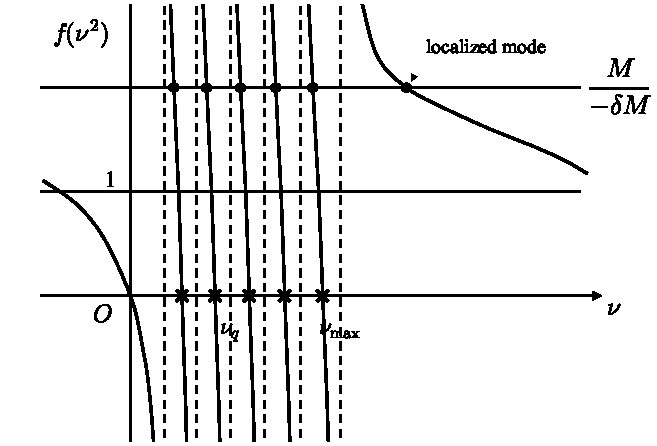
\includegraphics[width=0.72\textwidth]{fig_34.pdf}
\caption*{图 34\quad 对含同位素杂质的晶格的模，式 (2.143) 的图解求法。}
\end{figure}

这些根可以用作图法求得（图 34）。我们要找的是函数
\begin{equation*}
f(\nu^2)\equiv\frac{1}{N}\sum_{\mathbf{q}}\frac{\nu^2}{\nu^2-\nu^2_{\mathbf{q}}}
\tag{2.145}
\end{equation*}
与水平线 $(-M/\delta M)$ 相交的那些点。

例如，设 $\delta M$ 为负。(2.144) 的每个根必定位于 $f(\nu^2)$ 的某个极点 $\nu^2_{\mathbf{q}}$ 的上方；受扰系统的各简正模在频率上与完美晶体的各简正模交错排布。由于 $\nu_{\mathbf{q}}$ 的取值构成一个稠密的\emph{带}，其间隔像 $1/N$ 那样趋于零，新解中的大多数与原有的解无从区分。但是再看一眼图 34 就会注意到，最高的那个根并不受这种约束，它可以离开带的顶端 $\nu_{\max}$ 一段有限的距离。当 $\nu$ 大于 $\nu_{\max}$ 时，求和 (2.145) 可以近似地用对谱密度（spectral density）(2.65) 的一个积分来表示，即
\begin{equation*}
\bar{f}(\nu^2)=\int^{\nu^{\max}}\frac{\nu^2\mathcal{D}(\nu')}{\nu^2-\nu'^2}\,d\nu'.
\tag{2.146}
\end{equation*}
在这个函数等于 $(-M/\delta M)$ 的频率处，就出现一个与缺陷相联系的特殊模。

这个特殊模必定是\emph{局域}的。这来自一条普遍定理：\emph{晶格的振荡运动在简正模频谱之外的频率处，其波数为虚数}。以 §2.2 的线性链模型为例。若把 $q=i\kappa$ 代入 (2.16)，我们便解出了 (2.15)，其频率由 (2.18) 的类比式给出，即
\begin{equation*}
\nu_{\kappa}=\sqrt{\left(\frac{\alpha}{M}\right)}\;2\sinh\left(\frac{\kappa a}{2}\right),
\tag{2.147}
\end{equation*}
对 $\nu_{\kappa}$ 的任何取值它都能得到满足。当然，作为完美晶格的简正模，这个解析解在物理上是不允许的，因为位移振幅 $u_l$ 会沿链像 $\exp(\pm\kappa l)$ 那样指数式地增长或衰减，从而不能满足循环边界条件。然而在非完整晶体中，可以把缺陷邻域的条件安排成使振动振幅向四面八方衰减，于是在样品远处的边界上变得可以忽略。从物理上讲，图 34 中的杂质原子比晶体中周围的原子来得轻，它作独立“Einstein”振荡时的固有频率会比较高。观察到的就是位于扩展声子模带之上的一个简正模，其中只有少数几个近邻原子随杂质协同运动（图 35(a)）。

缺陷位置上局域振动的其他种种例子都可以类似地理解。例如，如果我们把某个原子周围的弹簧常量加硬一些，就会观察到同样的效应。另一方面，比平常更重一些的原子具有较低的 Einstein 频率，因此我们应当能看到一个局域模从某个正常频带之\emph{下}脱离出来——例如从双原子晶体的光学支中脱离出来。

说来也怪，表面模（surface modes）的理论竟循着同样的路数。当然，我们可以从经典弹性理论中搬用关于连续介质自由表面上 Rayleigh 波与 Love 波的标准讨论，或许还要对表面平面内波矢的大小加上一个 Debye 限制。但这些波对应于那些局域在表面上、并朝晶体内部指数式衰减的振动模。虽然离散晶格中相应的问题看上去非常复杂，

\begin{figure}[H]
\centering
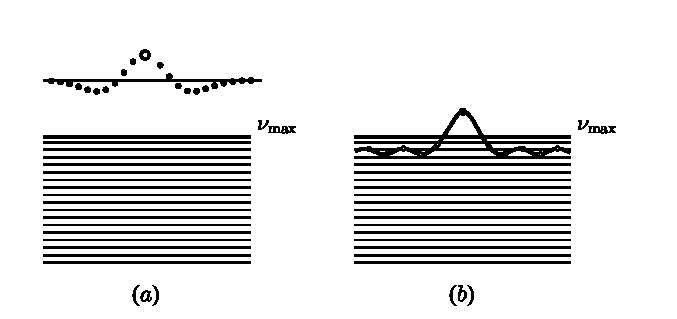
\includegraphics[width=0.72\textwidth]{fig_35.pdf}
\caption*{图 35\quad (a) 轻杂质在声子带之上的局域模。(b) 重杂质在声子带之内的共振模。}
\end{figure}

但若把系统处理成一列晶格平面——它们从表面平面处的一个重大缺陷（例如劲度为零的弹簧常量）出发，沿一维向晶体内部延伸——还是能学到许多东西。这样一来，这类模应当出现在双原子晶体中、声子谱的光学支与声学支之间的带隙里。表面模可能对微小晶粒的比热有可检测的贡献，并且在某些电子器件中很重要。

局域杂质模的特征频率可以通过红外波段的光吸收直接观测（见 §8.4）。而且，有意思的是，如果杂质的固有振动频率落在某个声子带之\emph{内}，也会产生一条有所展宽的吸收线——例如在 (2.143) 的简单同位素情形中取 $\delta M$ 为正。这是\emph{共振}（resonance）的一个例子；在峰频率处，振动振幅在杂质格点上要比晶体其余部分大得多，但它并不随距离指数式地消衰，因此不是严格局域的（图 35(b)）。不出所料，在这个频率上杂质对入射声子的散射也非常强烈。

事实上，共振的理论只不过是局域态理论的一种解析延拓。共振频率是 (2.144) 的解，只是把其中的求和 $f(\nu^2)$ 换成 $\bar{f}(\nu^2)$ 的积分 (2.146) 的主部；而共振的\emph{宽度}则由同一积分的虚部给出，只不过现在要在 $\nu<\nu_{\max}$ 的情形下取值。这类关系的证明通常是在“球对称势中量子力学粒子的 Schrödinger 方程之解”的语境下给出的，但这一论证普遍适用于连续介质和规则晶格中的波。

 % 本文件由 scripts/assemble.py 自动装配，勿手改（改 parts/ 后重跑）
% 第3章 电子态

% 第3章 Electron States
\chapter{电子态}

\epigraphbook{谱写部落歌谣的方法有六十九种，\\而其中每一种都无一不是对的。}{KIPLING}

\section{自由电子}

考察固体 Na。每个原子含有 11 个电子，但其中 10 个电子处于紧紧束缚在原子核上的状态，构成一个净正电荷为 $+|e|$ 的离子。在自由原子中，剩下的那个电子在围绕此离子的一个轨道（orbital）上运动。当诸原子聚集成固体时，这些轨道相互交叠并发生相互作用。可以论证，这种交叠是如此广泛，以致于把每个电子都定域在各自原子上的量子化方案必然失效，必须代之以另一种方案：每个电子的波函数是它在所有离子的势中运动的薛定谔方程（Schrödinger equation）的解。于是，我们一开始就区分两类电子：一类是芯电子（core electrons），它们被处理成几乎完全定域化的；另一类是价电子（valence electrons）或传导电子（conduction electrons），假定它们进入 Bloch 态——即延展于整个晶体之中的状态。

在本章中我们将采用单电子模型（one-electron model），即忽略价电子之间因库仑排斥而生的任何相互作用。这些关联（correlation）与交换（exchange）效应将在第 5 章中讨论。芯内部各电子之间、或芯电子与价电子之间的这类效应，通常被当作每个价电子在晶体中运动时所感受到的势 $\mathcal{V}(\mathbf{r})$ 的一部分来处理。于是，$\mathcal{V}(\mathbf{r})$ 被认为是按离子的 Hartree 势或 Hartree--Fock 势计算出来的。

如果假定 $\mathcal{V}(\mathbf{r})$ 是一个常数，就可以做一个极大的简化。这时电子便自动落入平面波态（plane-wave states）
\begin{equation*}
|{\bf k}\rangle=\psi_{\bf k}=e^{i{\bf k}\cdot{\bf r}},
\tag{3.1}
\end{equation*}
其能量为
\begin{equation*}
\mathcal{E}({\bf k})=\frac{\hbar^{2}k^{2}}{2m}.
\tag{3.2}
\end{equation*}

正如在 §1.5 中所见，这些态满足 Bloch 定理。等能面是 ${\bf k}$ 空间中的球面。${\bf k}$ 的允许值在此空间中以 $V/8\pi^{3}$ 的密度分布。但对每一个 ${\bf k}$ 值，实际上有两个电子态，自旋相反。如果实空间中单位体积内有 $ZN$ 个电子（即每个原子 $Z$ 个电子，每个晶胞 1 个原子，单位体积内有 $N$ 个晶胞），那么为了满足 Pauli 原理，我们需要把态一直填充到波数 $k_{F}$，$k_{F}$ 满足
\begin{align*}
\frac{4}{3}\pi k_{F}^{3}\,\frac{2}{8\pi^{3}}&=ZN,\\
\text{即}\quad k_{F}&=(3\pi^{2}ZN)^{1/3}.
\tag{3.3}
\end{align*}

\begin{figure}[H]
\centering
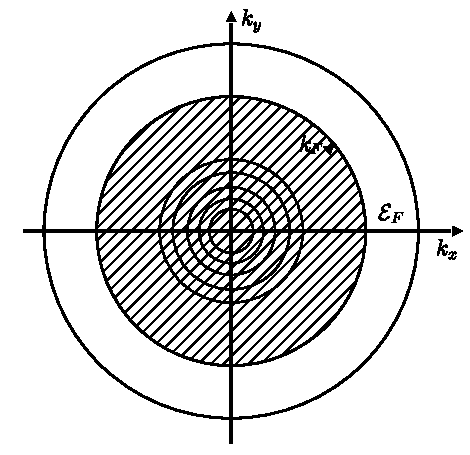
\includegraphics[width=0.72\textwidth]{fig_36.pdf}
\caption*{图 36\quad 自由电子的费米面。}
\end{figure}

我们说费米面（Fermi surface）是一个半径为 $k_{F}$ 的球面。费米能（Fermi energy）或费米能级（Fermi level）是相应于这一分布顶端的能量，
\begin{equation*}
\mathcal{E}_{F}=\frac{\hbar^{2}k_{F}^{2}}{2m}.
\tag{3.4}
\end{equation*}

我们注意到，费米球的半径与 Debye 球的半径相当。把式 (3.3) 与式 (2.53) 相比较，得
\begin{equation*}
k_{F}=\left(\frac{Z}{2}\right)^{1/3}q_{D}.
\tag{3.5}
\end{equation*}

这意味着费米能级上电子的波长与原子间距相当（参看式 (2.55)）：
\begin{equation*}
\lambda_{F}=\frac{2\pi}{k_{F}}\sim\left(\frac{2}{Z}\right)^{1/3}2.6\,r_{s},
\tag{3.6}
\end{equation*}
其中 $r_{s}$ 是 Wigner--Seitz 球的半径。

\section{价电子的衍射}

我们刚刚证明的结果使自由电子模型（free-electron model）露出了破绽：费米能级上的电子所处的态，其波长与晶格间距相当。因此必定存在强的衍射效应，即使 $\mathcal{V}(\mathbf{r})$ 与常数势没有非常显著的差别。让我们把这个势当作作用在自由电子态上的微扰来处理。令
\begin{equation*}
\mathcal{E}({\bf k})=\mathcal{E}_{\bf k}^{0}+\langle{\bf k}|\mathcal{V}|{\bf k}\rangle+\sum_{{\bf k}'}\frac{|\langle{\bf k}|\mathcal{V}|{\bf k}'\rangle|^{2}}{\mathcal{E}_{\bf k}^{0}-\mathcal{E}_{{\bf k}'}^{0}},
\tag{3.7}
\end{equation*}
其中
\begin{equation*}
\mathcal{E}_{\bf k}^{0}\equiv\hbar^{2}k^{2}/2m,
\tag{3.8}
\end{equation*}
并且对势在未微扰态 (3.1) 之间的矩阵元采用了 Dirac 记号。

但 $\mathcal{V}(\mathbf{r})$ 必须具有晶格的周期性。如 §2.6 中所证明，除非 $({\bf k}-{\bf k}')$ 是一个倒格矢（reciprocal lattice vector），否则它的矩阵元为零。由式 (2.78) 立即得到
\begin{equation*}
\mathcal{E}({\bf k})=\mathcal{E}_{\bf k}^{0}+\mathcal{V}_{0}+\sum_{{\bf g}\neq{\bf 0}}\frac{|\mathcal{V}_{\bf g}|^{2}}{\mathcal{E}_{\bf k}^{0}-\mathcal{E}_{\bf k-{\bf g}}^{0}},
\tag{3.9}
\end{equation*}
其中 $\mathcal{V}_{\bf g}$ 是 $\mathcal{V}$ 对应于倒格矢 ${\bf g}$ 的 Fourier 分量（如式 (1.15)）。

问题在于——这样一个展开究竟有多好？有两个条件必须满足：(i) 当 ${\bf g}$ 增大时，Fourier 分量 $\mathcal{V}_{\bf g}$ 应当迅速趋于零；(ii) 在被微扰所混合的诸未微扰态之间，不得存在如下形式的简并
\begin{equation*}
\mathcal{E}_{\bf k}^{0}=\mathcal{E}_{\bf k-{\bf g}}^{0}
\tag{3.10}
\end{equation*}
目前，先把条件 (i) 搁置，留待以后研究。

简并条件 (3.10) 等价于写成
\begin{equation*}
|{\bf k}|=|{\bf k}-{\bf g}|;
\tag{3.11}
\end{equation*}
从几何上看，这意味着 ${\bf k}$ 位于倒格矢 ${\bf g}$ 的垂直平分面上。也就是说——\emph{当 ${\bf k}$ 位于（或接近）区边界时，简单的微扰展开式 (3.9) 便不再有效}。这个公式只能在未微扰态的球面未触及区的边界时使用——实际上，即使对单价金属，它也很少有效。

\begin{figure}[H]
\centering
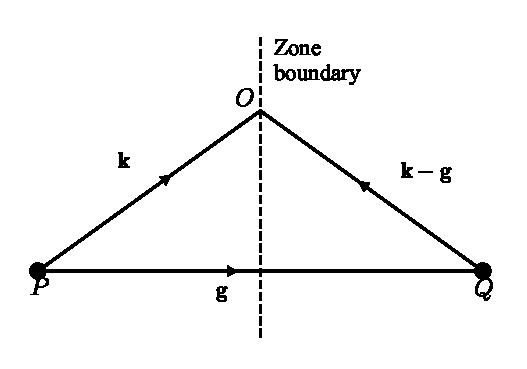
\includegraphics[width=0.72\textwidth]{fig_37.pdf}
\caption*{图 37\quad （原书此图无图注。）}
\end{figure}

注意，图 37 正是波矢为 ${\bf k}$ 的电子相干 Bragg 衍射到方向 ${\bf k}'={\bf k}-{\bf g}$ 的 Ewald 作图（图 29(b)）。在每一种情形下，几何条件都是：$OPQ$ 应构成一个等腰三角形，且以倒格矢 ${\bf g}$ 为底边 $PQ$。于是我们从代数上证实：晶体内的价电子受到来自晶格的衍射作用，恰好像它们是从晶体外部入射进来的一样。

为了求出区边界邻域内的解，我们必须显式地考察微扰方程。晶格的周期性意味着势只能混合相差一个倒格矢 ${\bf g}$ 的波，因此我们是假定波函数可以展开成级数
\begin{equation*}
\psi_{\bf k}=\sum_{\bf g}\alpha_{\bf k-{\bf g}}e^{i({\bf k}-{\bf g})\cdot{\bf r}}.
\tag{3.12}
\end{equation*}
若把它代入薛定谔方程
\begin{equation*}
\left\{-\frac{\hbar^{2}}{2m}\nabla^{2}+\mathcal{V}(\mathbf{r})\right\}\psi_{\bf k}=\mathcal{E}({\bf k})\psi_{\bf k},
\tag{3.13}
\end{equation*}
并用展开式中的某一项去乘遍整个方程，便得到系数 $\alpha$ 的线性方程组：
\begin{equation*}
\{\mathcal{E}_{\bf k-{\bf g}}^{0}-\mathcal{E}({\bf k})\}\alpha_{\bf k-{\bf g}}+\sum_{{\bf g}'}\mathcal{V}_{{\bf g}-{\bf g}'}\alpha_{\bf k-{\bf g}'}=0
\tag{3.14}
\end{equation*}
其中 ${\bf g}$ 取一切值（包括 ${\bf g}={\bf 0}$ 和 ${\bf g}'={\bf 0}$）。众所周知，只须假定除 $\alpha_{\bf k}$ 之外所有 $\alpha_{\bf k-{\bf g}}$ 都很小，便可由此得到简单的微扰公式 (3.9)。实际上，这时我们取
\begin{equation*}
\alpha_{\bf k-{\bf g}}\approx\frac{\mathcal{V}_{-{\bf g}}}{\mathcal{E}_{\bf k}^{0}-\mathcal{E}_{\bf k-{\bf g}}^{0}}.
\tag{3.15}
\end{equation*}

当 ${\bf k}$ 位于某条区边界附近时——比如说平分矢量 ${\bf G}$ 的那条边界——恰恰就是这个假定失效了。波 $\exp\{i({\bf k}-{\bf G})\cdot{\bf r}\}$ 的系数变得与原来未微扰态的系数同等重要。实际上，此时电子已被晶格作了 Bragg 反射，就好像它是一束从外部入射的电子束一样。条件 (3.11) 等价于 §2.6 中的式 (2.79) 和 (2.80)。为了构成一个定态，我们必须把入射束和衍射束放在同等的地位上处理。

作为近似，让我们忽略 (3.14) 中除这两个系数之外的所有系数。把能量原点移动 $\mathcal{V}_{0}$ 之后，得到
\begin{equation*}
\left.\begin{aligned}
\{\mathcal{E}_{\bf k}^{0}-\mathcal{E}({\bf k})\}\alpha_{\bf k}+\mathcal{V}_{\bf G}\alpha_{\bf k-{\bf G}}&=0,\\
\mathcal{V}_{-{\bf G}}\alpha_{\bf k}+\{\mathcal{E}_{\bf k-{\bf G}}^{0}-\mathcal{E}({\bf k})\}\alpha_{\bf k-{\bf G}}&=0.
\end{aligned}\right\}
\tag{3.16}
\end{equation*}

方程组的行列式是 $\mathcal{E}({\bf k})$ 的一个二次式，其解为
\begin{equation*}
\mathcal{E}^{\pm}({\bf k})=\tfrac{1}{2}(\mathcal{E}_{\bf k}^{0}+\mathcal{E}_{\bf k-{\bf G}}^{0})\pm\tfrac{1}{2}\sqrt{(\mathcal{E}_{\bf k}^{0}-\mathcal{E}_{\bf k-{\bf G}}^{0})^{2}+4|\mathcal{V}_{\bf G}|^{2}}
\tag{3.17}
\end{equation*}
（注意到 $\mathcal{V}_{-{\bf G}}=\mathcal{V}_{\bf G}^{*}$）。这样，态 $e^{i{\bf k}\cdot{\bf r}}$ 与 $e^{i({\bf k}-{\bf G})\cdot{\bf r}}$ 组合成另外两个态 $\psi^{+}$ 和 $\psi^{-}$，其能量分别为 $\mathcal{E}^{+}$ 和 $\mathcal{E}^{-}$。

为简单起见，让我们考虑在一维情形下会发生什么。在 $k=0$ 附近，两个未微扰能量之差大得很，以致我们可以忽略 $4|\mathcal{V}_{\bf G}|^{2}$。我们得到
\begin{equation*}
\mathcal{E}({\bf k})\sim\mathcal{E}_{\bf k}^{0},
\tag{3.18}
\end{equation*}
因而 $\psi^{-}$ 沿着自由电子抛物线。在 $k=\frac{1}{2}G$ 处，也就是区边界处，两个未微扰波具有相同的能量：于是
\begin{equation*}
\mathcal{E}^{-}(\tfrac{1}{2}G)=\mathcal{E}_{\frac{1}{2}G}^{0}-|\mathcal{V}_{\bf G}|.
\tag{3.19}
\end{equation*}
（译注：原书此式右端误印为“$+$”，按式 (3.17) 及上下文“$\psi^{-}$ 的能量被压低”应为“$-$”。）态 $\psi^{-}$ 的能量比自由电子抛物线低了一个量 $|\mathcal{V}_{\bf G}|$。我们在图 38 中的 $A$ 点看到这一点。

\begin{figure}[H]
\centering
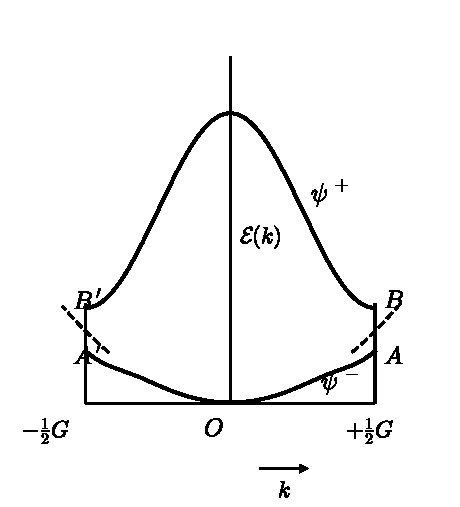
\includegraphics[width=0.72\textwidth]{fig_38.pdf}
\caption*{图 38\quad 一维情形的电子能量：简约区图式。}
\end{figure}

在区边界处，态 $\psi^{+}$ 具有能量
\begin{equation*}
\mathcal{E}^{+}(\tfrac{1}{2}G)=\mathcal{E}_{\frac{1}{2}G}^{0}+|\mathcal{V}_{\bf G}|,
\tag{3.20}
\end{equation*}
因而它的能量被抬高到自由电子抛物线之上。若把 $k$ 限制在区之内，我们发现随着 $k$ 的减小，这个态的能量趋于 $\mathcal{E}_{\bf k-{\bf G}}^{0}$。这样，区内的能量便落入两个\emph{能带}（band），中间隔着宽度为 $2|\mathcal{V}_{\bf G}|$ 的带隙（gap）$AB$。

把图 38 与 §1.5 中的图 14 加以比较是有启发性的。那个颇为人为的自由电子简约区图式（reduced zone scheme），已经被周期性晶格势分裂成若干个能带。我们也可以用另一种方式来表示这个结果：把 $\psi^{+}$ 这一支画到第二个区中去——即采用扩展区图式（extended zone scheme）（图 39）。这样更清楚地表明，各个能量是如何由自由电子抛物线经微扰而得出的——只是在区边界处引入了不连续性。这同我们在 §2.2 的图 19(c) 中观察到的现象一样，在那里，两种不同质量的引入使晶格的振动谱发生了分裂。

\begin{figure}[H]
\centering
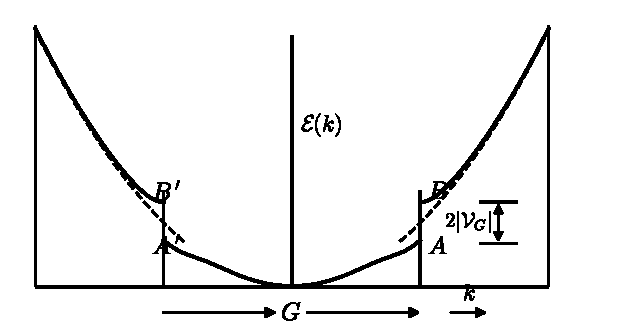
\includegraphics[width=0.72\textwidth]{fig_39.pdf}
\caption*{图 39\quad 一维情形的电子能量：扩展区图式。}
\end{figure}

为了理解所发生的事情，让我们计算 $k=\frac{1}{2}G$ 处的波函数。假定 $\mathcal{V}_{\bf G}$ 为负。由式 (3.12) 和 (3.16) 我们得到
\begin{align*}
\psi^{-}&=(e^{i\frac{1}{2}Gr}+e^{-i\frac{1}{2}Gr})/\sqrt{2}\\
&=\sqrt{2}\cos\tfrac{1}{2}Gr
\tag{3.21}
\end{align*}
以及
\begin{equation*}
\psi^{+}=\sqrt{2}\,i\sin\tfrac{1}{2}Gr.
\tag{3.22}
\end{equation*}

因此，$|\psi^{-}|^{2}$ 是这样一个函数：它在 $r=0$ 附近很大，而且也在
格点处。它对应于电子集中分布在原子上的状态。但这正是我们所预期的。$\mathcal{V}_{G}$ 的\emph{负}值对应于在每个原子邻域内为负的周期势——一个\emph{吸引}电子的势。这样，$\psi^{-}$ 由于与原子的势阱相配合，能量被降低；类似地，$\psi^{+}$ 的能量被升高，因为它使电子密度在正势区域变大。仿照原子轨道的称谓，我们说 $\psi^{-}$ 是 $s$ 型的，$\psi^{+}$ 是 $p$ 型的。

顺便指出，展开式 (3.12) 使 $\psi_{\mathbf{k}}$ 能够满足 Bloch 定理 (1.58)。我们可以写成
\begin{align*}
\psi_{\mathbf{k}} &= e^{i\mathbf{k}\cdot\mathbf{r}}\sum_{\mathbf{g}}\alpha_{\mathbf{k}-\mathbf{g}}e^{-i\mathbf{g}\cdot\mathbf{r}}\notag \\
&= e^{i\mathbf{k}\cdot\mathbf{r}}u_{\mathbf{k}}(\mathbf{r}), \tag{3.23}
\end{align*}
其中 $u_{\mathbf{k}}(\mathbf{r})$ 是晶格中的周期函数，正如 (1.60) 中那样。

\begin{figure}[H]
\centering
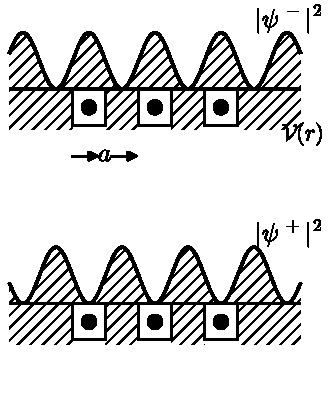
\includegraphics[width=0.72\textwidth]{fig_40.pdf}
\caption*{图 40\quad 周期势，以及 $s$ 型与 $p$ 型态中的电子密度。}
\end{figure}

我们还注意到，图 39 中 $A$ 与 $A'$ 两处的波函数是完全相同的；二者均由 (3.21) 给出。类似地，$\psi^{+}(\frac{1}{2}G)$ 与 $\psi^{+}(-\frac{1}{2}G)$ 除相差一个常数外也相同，因此 $B$ 与 $B'$ 两点在图 38 与图 39 的区图式中是等价的。这是 §1.5 中所讨论的那些原理的一个实例，在那里已经证明：一个态的波矢量在相差一个倒格矢的意义下是任意的。

\section{近自由电子模型}

一维情形的这些原理可以推广到三维。如果我们沿着 k 空间中某个特定方向考察 $\mathcal{E}(\mathbf{k})$ 的行为，就会发现它沿着一条自由电子抛物线变化，而在穿过布里渊区边界时发生跳跃式的不连续（图 41）。每个不连续的大小将取决于势中相应 Fourier 分量的强弱。如果区边界是倒格矢 $\mathbf{G}$ 的垂直平分面，那么不连续的大小将是 $2|\mathcal{V}_{\mathbf{G}}|$ 的量级。每当一条等能线穿过区边界时，同样会出现这种不连续。于是（图 42），本应穿过 $O$ 点的自由电子球被分裂成双曲面的一叶——在区内 $S$ 处，由 (3.17) 的一个根生成——以及边界之外另一支的一叶 $S'$。

\begin{figure}[H]
\centering
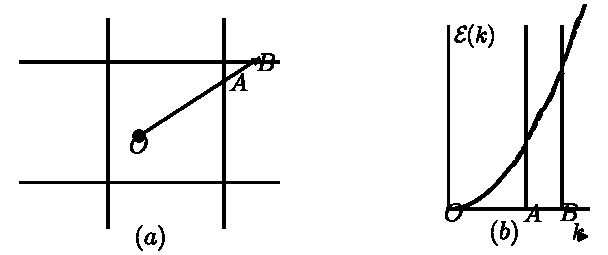
\includegraphics[width=0.72\textwidth]{fig_41.pdf}
\caption*{图 41\quad 沿 k 空间中的 $OAB$ 线，在区边界处 $\mathcal{E}(\mathbf{k})$ 出现不连续。}
\end{figure}

\begin{figure}[H]
\centering
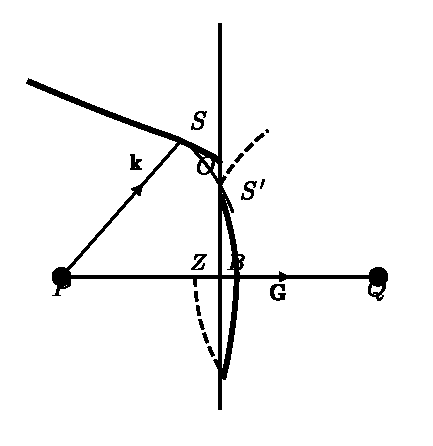
\includegraphics[width=0.72\textwidth]{fig_42.pdf}
\caption*{图 42\quad 区边界处等能线的不连续。}
\end{figure}

这意味着函数 $\mathcal{E}(\mathbf{k})$ 在第一布里渊区内部是连续的——但在任何一点越过区边界时，能量都有一个跳跃。这使该理论最引人注目的推论之一成为可能：\emph{对某些能量值，可能不存在电子态}。能谱可以出现能隙。电子能级分成了若干\emph{能带}。这是一条基本性质，它衍生出金属和半导体的许多性质。它是 Bragg 衍射的一个后果。电子波函数被“拉”得与晶格具有相同的周期性，并在能量上分裂开来。

目前我们关心的是求出 $\mathcal{E}(\mathbf{k})$ 的问题。上一节的计算提示了如下的方法：——用方程组 (3.14) 求展开式 (3.12) 中系数的解；把所有与能被 $\mathbf{k}$ 附近的区边界所混合的波的系数相对应的项分离出来，对能量 $\mathcal{E}(\mathbf{k})$ 求解久期行列式（secular determinant）；再用形如 (3.9) 的微扰展开修正势的其他 Fourier 分量的效应。

这称为\emph{近自由电子}（nearly-free-electron，N.F.E.）方法。要使它有效，Fourier 分量 $\mathcal{V}_{\mathbf{g}}$ 的级数应当迅速收敛。可是乍看起来这一点似乎不大可能。$\mathcal{V}(\mathbf{r})$ 是离子阵列的势。我们知道，离子核心附近的场非常强——$\mathcal{V}(\mathbf{r})$ 在每个格点处都有一个向下延伸的长而尖的尖峰。这意味着它具有波长非常短的 Fourier 分量，因此当 $\mathbf{g}$ 为第一区尺度的许多倍时，$\mathcal{V}_{\mathbf{g}}$ 仍可能很大。或者我们也可以说，$\psi_{\mathbf{k}}(\mathbf{r})$ 在离子核心内部必须表现得像原子轨道一样，带有对应于高动能的多次振荡。这同样意味着，在表示式 (3.12) 中我们需要许多项，一直用到非常短的波长。

正是这些论证曾使这一方法作为能带结构的实用计算方案而遭到忽视。但现在看来，通过引入赝势（pseudo-potential）的观念，可以使它在形式上有效。这将由 §3.6 展开。

N.F.E. 模型作为说明函数 $\mathcal{E}(\mathbf{k})$ 在 k 空间中行为的手段非常有用。考虑一个矩形点阵——二维情形——它的倒格子也是矩形的，如图 43 所示。第一布里渊区很容易构造——就是矩形 $RR'R''R'''$。$\mathcal{E}(\mathbf{k})$ 在此区内部必须连续，而且在勾画这个晶胞的任何一条线上都可能出现不连续。

但再考虑中央区之外 $\mathcal{E}(\mathbf{k})$ 不连续点的轨迹。它们可以是倒格子中任一矢量的垂直平分线。因此，图中任何一条线上都可能有不连续——例如 $\mathbf{g}_{3}$ 的垂直平分线就是一条穿过区角隅的对角线。我们最初那张关于不连续的图（图 41）是不对的——它没有画出可能发生的一切，即便是方格子情形也不例外。因此，在图 43 中的 $X_{1},X_{2},X_{3},X_{4}$ 等点处，$\mathcal{E}(\mathbf{k})$ 都可能有跳跃和能隙。

\begin{figure}[H]
\centering
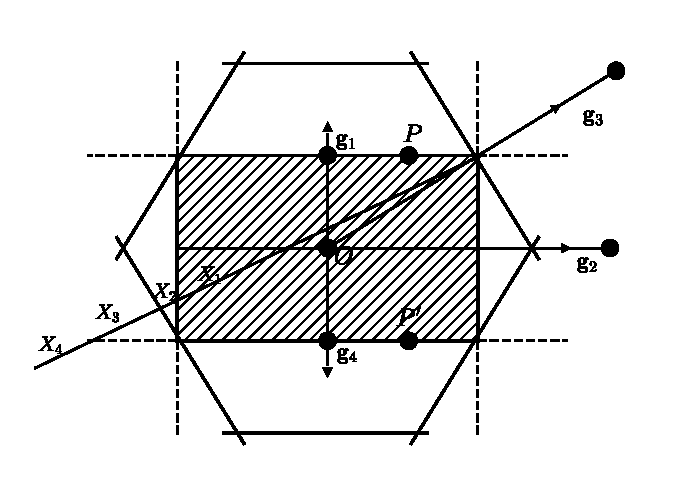
\includegraphics[width=0.72\textwidth]{fig_43.pdf}
\caption*{图 43\quad 在矩形倒格子中，$\mathcal{E}(\mathbf{k})$ 的不连续将出现在 $X_{1}$、$X_{2}$、$X_{3}$、$X_{4}$ 处。}
\end{figure}

这看起来似乎表明 $\mathcal{E}(\mathbf{k})$ 是一个远比实际情形复杂的函数。例如，假定我们试着画出由 N.F.E. 模型得出的一些等能线。它们看上去将如图 44 那样（把注意力限定在这些平面组以内的区域）。我们可以先画出自由电子圆，再按图 42 所示的方式加入不连续，从而把它们构造出来。或者更确切地说，我们应当对该点处相互混合的那些波的能量求解久期行列式。于是在 $P$ 点有与 $P'$ 处的波的混合，因为在自由电子方案中这两点能量相同，且相差一个倒格矢。类似地，为求 $Q$ 点的解，我们需要考虑这样一个 $3\times 3$ 行列式，它描述波矢本应为 $OQ$、$OQ'$ 和 $OQ''$ 的那些波（在自由电子模型中）的混合。

现在的意思是，在 $P$ 与 $P'$ 两点我们将求解的是完全相同的方程。两点的能级相同。我们将其中的较低者归属于第一区内部；在每种情形下，较高的能级都属于区边界之外的等能线。同样，在 $Q$、$Q'$ 和 $Q''$ 处方程也是同一个，并给出三个能量根。我们可以把其中的最低者，在这些点的每一处，归属于图 44 中各边界以内的区域。于是这三个点能量全部相同。我们可以考察这些点的邻域，并类似地证明：$A$ 与 $A'$、$B$ 与 $B'$、$C$ 与 $C'$ 都是在此意义下等价的点对；$A$ 与 $A'$ 是同一波函数的两套可互换的标记，借助倒格子平移即可相互还原。

\begin{figure}[H]
\centering
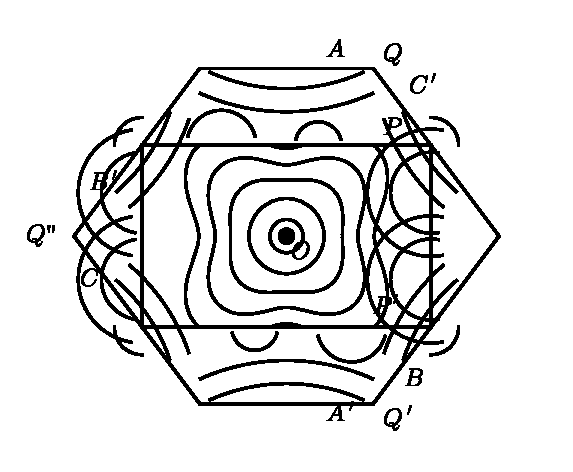
\includegraphics[width=0.72\textwidth]{fig_44.pdf}
\caption*{图 44\quad 矩形区中的等能线。}
\end{figure}

现在看一看，当我们用倒格矢把第一区之外的那些碎块零料平移过去时会发生什么。它们完美地拼合起来，构成单一的区——在 Brillouin 扩展区图式中，这些部分本来都被说成属于\emph{第二区}。而且，边界上的等价点恰好匹配，使等能线连续起来。\emph{简约区中的能量是 $\mathbf{k}$ 的连续函数}。

我们表示能面的方案于是就像图 46 那样，每条能带配一个区。我们可以把这些等能线想成不同曲面的等高线；把它们一层层堆叠起来，就可以把 $\mathcal{E}(\mathbf{k})$ 表示成简约区中 $\mathbf{k}$ 的多值函数，而不必像扩展区图式中那样让 $\mathcal{E}(\mathbf{k})$ 成为单值函数。

我们还可以再进一步。可以证明（我们的 N.F.E. 模型就能提供一个证明），在每条能带之内 $\mathcal{E}(\mathbf{k})$ 是连续的，且导数也连续。图 45 中画出的那些内部边界在能面上并不显现；等能线平滑地从它们上面越过。现在让我们回想，基本区本身就是倒格子的晶胞，通过倒格子平移可以把它重复排列，产生布满全空间的图案。而且，像 $P$ 与 $P'$ 这样原本等价、因而代表同一状态和相同能量的点，现在相互重合，于是 $\mathcal{E}(\mathbf{k})$ 跨越这些边界也是连续的。可以证明，等能线从一个晶胞到下一个晶胞平滑地衔接。于是，\emph{给定能带中的能量是 $\mathbf{k}$ 的具有倒格子周期的连续函数}。我们把它称为重复区图式（repeated zone scheme）。这与我们在 §2.2 中就恒定晶格频率曲面所观察到的原理如出一辙。

\begin{figure}[H]
\centering
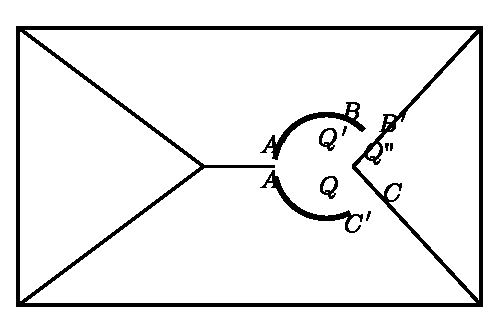
\includegraphics[width=0.72\textwidth]{fig_45.pdf}
\caption*{图 45\quad 约化成单一的区。}
\end{figure}

\begin{figure}[H]
\centering
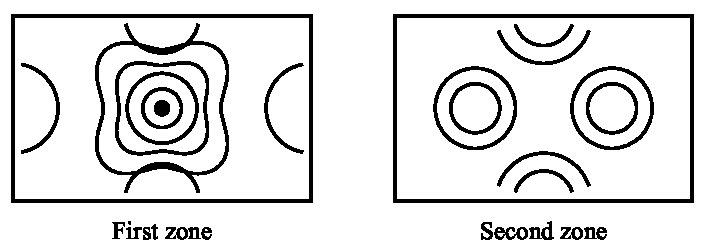
\includegraphics[width=0.72\textwidth]{fig_46.pdf}
\caption*{图 46\quad 对应于图 44 的简约区图式。}
\end{figure}

这一原理的一个有趣应用，是 Harrison 的方法：在重复区图式中构造价为 $Z$ 的金属的费米面。设 N.F.E. 方案中的微扰势非常小。此时能量面必定是球面。我们算出体积恰为一个区的 $\frac{1}{2}Z$ 倍的球面的半径，并以原点为中心把它画出。再围绕倒格子的每一点画出同样的球面，于是便得到一幅具有重复区图式周期性的图案（图 48）。

现在，我们可以从这幅图案中挑出各种能够连续拼合的部分，组成在每个区中都重复的曲面。这些分立的图形，每一个便构成费米面的一个分支，即费米面在第 1、第 2、第 3……区中的部分（图 49）。当作球面画出时，这些曲面在各部分相接处看似带有尖点，但与势的 Fourier 分量相联系的态的混合会把棱角磨圆，给出光滑的几何对象。正如我们将在第 9 章看到的那样，所得的曲面往往与实验上可观察到的曲面相当相像，而且对于研究复杂金属中的费米面，它们肯定提供了宝贵的指引。

\begin{figure}[H]
\centering
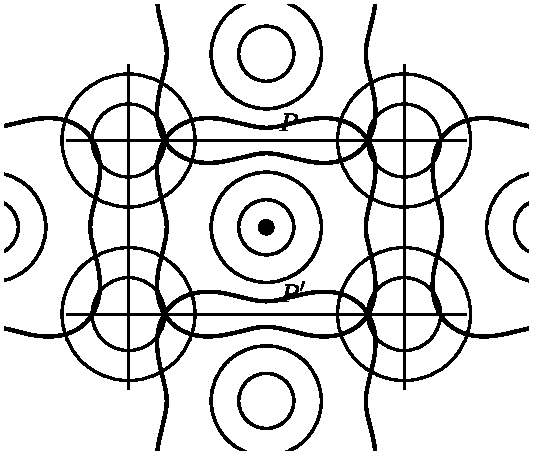
\includegraphics[width=0.72\textwidth]{fig_47.pdf}
\caption*{图 47\quad 对应于图 46 的重复第一区。}
\end{figure}

\begin{figure}[H]
\centering
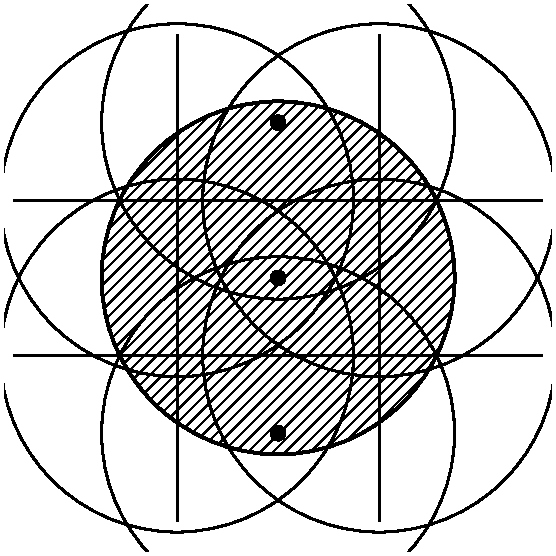
\includegraphics[width=0.72\textwidth]{fig_48.pdf}
\caption*{图 48\quad 自由电子费米面的 Harrison 作图。}
\end{figure}

这些代数公式和几何构图也出现在动力学衍射理论（dynamical theory of diffraction）中（§2.6）。在非常接近衍射条件 (3.11) 时，穿过晶格的快电子束或 X 射线束就不再能表示成带单一波矢 $\mathbf{k}$ 的简单平面波。各种衍射波必须像 (3.12) 那样包括进波函数之中，从而改变了
%（句子未完，下接书页 91 / p105 页首 "excitation."——应续作“……从而改变了激发的速度”，由下一部分的 B-TAIL 续译。）

\begin{figure}[H]
\centering
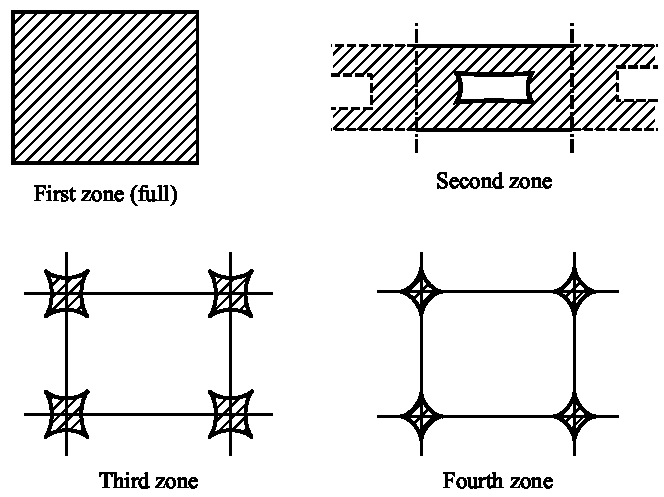
\includegraphics[width=0.72\textwidth]{fig_49.pdf}
\caption*{图 49\quad 对应于图 48 的简约区：第一区（满）、第二区、第三区、第四区。}
\end{figure}

\begin{figure}[H]
\centering
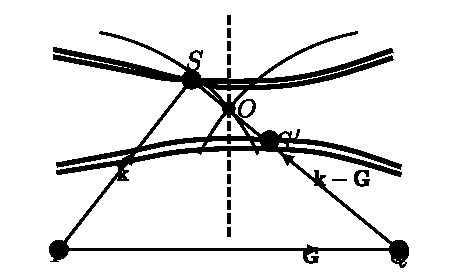
\includegraphics[width=0.72\textwidth]{fig_50.pdf}
\caption*{图 50\quad X 射线或快电子动力学衍射的色散面。}
\end{figure}
速度。例如，在简单的区边界附近，至少必须把两支波组合起来，得到一个类似于式 (3.17) 的二次方程，它给出电子或光子能量作为 $\mathbf{k}$ 的函数的两个根。

这些根生成了图 50 中的\emph{色散面}。原先以倒格点 $P$ 与 $Q$ 为中心、半径为 $\nu/c$ 的“自由光子”球面本应在区边界上的 $O$ 点相交（参看图 29 与图 37），如今则分裂成两个双曲面。因此，图中诸如 $S$ 或 $S'$ 这样的点代表一个频率为 $\nu$ 的电磁扰动，它以两支平面波的组合形式在晶体中传播，其波矢为 $SP$ 与 $SQ$，或 $S'P$ 与 $S'Q$。为了与这个频率的入射 X 射线相匹配，色散面两个分支的波束都被激发，从而导致 §2.6 中提到过的干涉效应。除了尺度上的差别——X 射线或快电子的波矢通常远大于倒格子的典型矢量——图 50 其实与图 42 完全相同。

\section{紧束缚法}

N.F.E. 方法着眼于原子芯以外的波函数，它们看上去非常像平面波；而在芯区内，它们则像原子轨道。这提示了一种截然不同的电子波函数构造方案：我们试着把各自局域在特定原子上的原子轨道组合起来，用以表示一个贯穿整个晶体的状态。

设 $\phi_a(\mathbf{r}-\mathbf{l})$ 是中心位于 $\mathbf{l}$ 处的自由原子的一个原子轨道。于是我们可以构造一个满足 Bloch 条件 (1.58) 的函数
\begin{equation*}
\phi_{\mathbf{k}}(\mathbf{r})=\sum_{l}e^{i\mathbf{k}\cdot\mathbf{l}}\phi_a(\mathbf{r}-\mathbf{l}).
\tag{3.24}
\end{equation*}
这个函数看起来像一列强局域化的原子轨道，乘上一个波动的相位因子 $\exp(i\mathbf{k}\cdot\mathbf{l})$。在每个原子内部，局域轨道占主导，应当是局域 Schr\"odinger 方程的一个很好的解。

作为一级近似，让我们对这个波函数计算能量的期望值
\begin{equation*}
\mathcal{E}(\mathbf{k})=\frac{\displaystyle\int\phi_{\mathbf{k}}^{*}\left\{-\frac{\hbar^{2}}{2m}\nabla^{2}+\mathcal{V}(\mathbf{r})\right\}\phi_{\mathbf{k}}\,\mathrm{d}\mathbf{r}}{\displaystyle\int\phi_{\mathbf{k}}^{*}\phi_{\mathbf{k}}\,\mathrm{d}\mathbf{r}}.
\tag{3.25}
\end{equation*}

\begin{figure}[H]
\centering
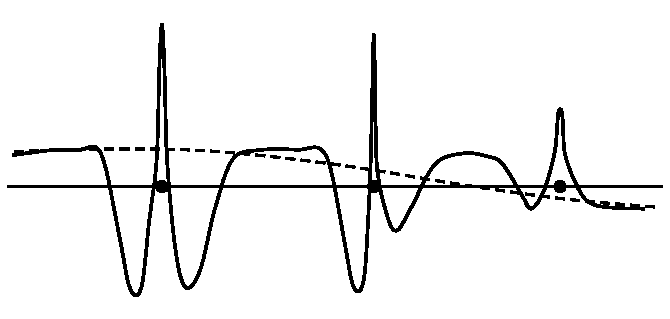
\includegraphics[width=0.72\textwidth]{fig_51.pdf}
\caption*{图 51\quad 固体中的波函数}
\end{figure}

如果相邻晶胞中轨道的交叠不太大，我们或许可以把分母中的归一化因子取为 1。分子可以写成
\begin{align*}
\mathcal{E}(\mathbf{k})&\approx\sum_{ll'}e^{i\mathbf{k}\cdot(\mathbf{l}-\mathbf{l}')}\int\phi_a^{*}(\mathbf{r}-\mathbf{l}')\left\{-\frac{\hbar^{2}}{2m}\nabla^{2}+\mathcal{V}(\mathbf{r})\right\}\phi_a(\mathbf{r}-\mathbf{l})\,\mathrm{d}\mathbf{r}\\
&=\sum_{\mathbf{h}}e^{i\mathbf{k}\cdot\mathbf{h}}\mathcal{E}_{\mathbf{h}},
\tag{3.26}
\end{align*}
其中
\begin{equation*}
\mathcal{E}_{\mathbf{h}}=\frac{1}{v_c}\int\phi_a^{*}(\mathbf{r}+\mathbf{h})\left\{-\frac{\hbar^{2}}{2m}\nabla^{2}+\mathcal{V}(\mathbf{r})\right\}\phi_a(\mathbf{r})\,\mathrm{d}\mathbf{r}.
\tag{3.27}
\end{equation*}
我们利用晶格势的周期性，使各个积分只依赖于轨道所居格点的相对位置 $\mathbf{h}=\mathbf{l}-\mathbf{l}'$。

现在设 $\phi_a(\mathbf{r})$ 满足方程
\begin{equation*}
\left\{-\frac{\hbar^{2}}{2m}\nabla^{2}+v_a(\mathbf{r})\right\}\phi_a(\mathbf{r})=\mathcal{E}_a\phi_a(\mathbf{r}),
\tag{3.28}
\end{equation*}
其中 $v_a(\mathbf{r})$ 现在是位于 $\mathbf{r}=\mathbf{0}$ 处的孤立原子的势。

\begin{figure}[H]
\centering
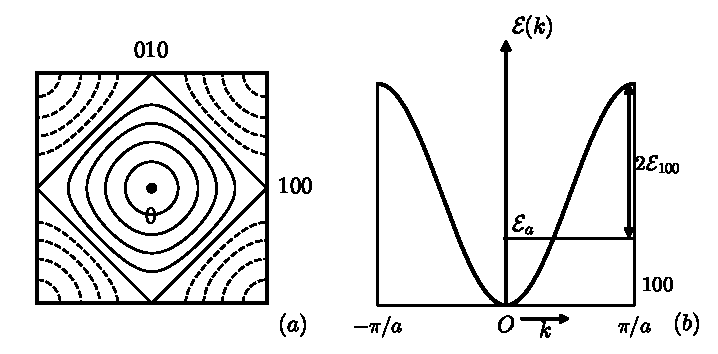
\includegraphics[width=0.72\textwidth]{fig_52.pdf}
\caption*{图 52\quad (a)等能线；(b)紧束缚法得到的沿立方轴的 $\mathcal{E}(k)$}
\end{figure}

如果我们略去各种交叠积分，便得到
\begin{equation*}
\left.\begin{aligned}
\mathcal{E}_{0}&\approx\mathcal{E}_a,\\
\mathcal{E}_{\mathbf{h}}&\approx\frac{1}{v_c}\int\phi_a^{*}(\mathbf{r}+\mathbf{h})\left\{\mathcal{V}(\mathbf{r})-v_a(\mathbf{r})\right\}\phi_a(\mathbf{r})\,\mathrm{d}\mathbf{r}.
\end{aligned}\right\}
\tag{3.29}
\end{equation*}
显然，$\phi_a(\mathbf{r}+\mathbf{h})$ 与 $\phi_a(\mathbf{r})$ 之间必须有某种交叠，$\mathcal{E}_{\mathbf{h}}$ 才不至于为零——而 $\mathbf{h}$ 处原子附近的高势会增强这种交叠。但是我们可以预期，除了近邻以外，$\mathcal{E}_{\mathbf{h}}$ 都应当非常小。

考虑一个简单立方晶格，取 $\mathbf{h}=(a,0,0)$ 等等。于是，当 $\phi_a(\mathbf{r})$ 具有立方对称性时，
\begin{equation*}
\mathcal{E}(\mathbf{k})\approx\mathcal{E}_a+2\mathcal{E}_{100}(\cos ak_x+\cos ak_y+\cos ak_z),
\tag{3.30}
\end{equation*}
这个情形下的区当然是一个立方体，能面如图 52 所示。由式 (3.29) 易见 $\mathcal{E}_{100}$ 本质上是负的。我们得到一条宽度为 $12|\mathcal{E}_{100}|$ 的能带，其最低能量为 $\mathcal{E}_a+6\mathcal{E}_{100}$。

沿立方轴方向我们看到，$\mathcal{E}(\mathbf{k})$ 在 $k=0$ 处有一个极小，而在区边界 $\mathbf{k}=(\pi/a,0,0)$ 处有一个极大。这与 N.F.E. 模型的曲线（图 36）表面上有几分相似，但带底的曲率依赖于 $\mathcal{E}_{100}$。整条能带的结构依赖于诸如式 (3.29) 那样的积分，它们对原子芯之外轨道的细节以及晶格间距都非常敏感。显然，如果原子轨道高度局域化，或者晶格间距变大，能带将趋于变得非常窄。

这种\emph{紧束缚法}演示了一条重要的原理。设想我们取 $N$ 个原子，并让它们彼此相距很远。每个原子上将有各不相同的原子能级 $\phi_a,\phi_b,\phi_c$；而在整个集合中，对单个电子来说，这些将是 $N$ 重简并的状态。

\begin{figure}[H]
\centering
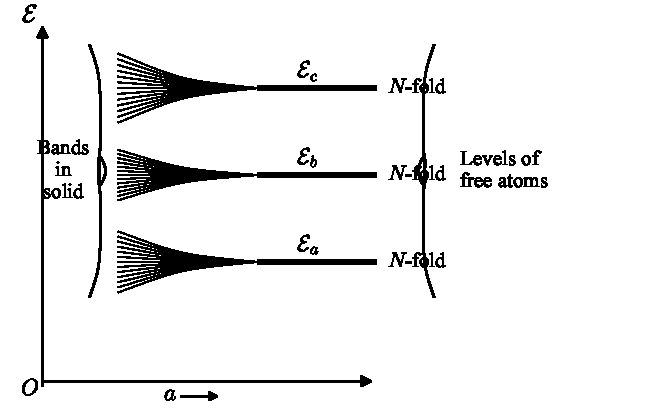
\includegraphics[width=0.72\textwidth]{fig_53.pdf}
\caption*{图 53\quad 原子彼此靠拢时，原子能级展宽成带}
\end{figure}

但当我们把原子聚到一起时，轨道发生交叠——于是我们发现，$N$ 重简并被劈裂成一个态带。每一条原子能级都将产生一个完整的、含 $N$ 个态的能带——因此我们可以谈及由相应原子态产生的 3s 带、4p 带等等。这种分类在过渡金属的情形下特别贴切：原子的 d 态在每个芯内都相当紧致，因而它们组合成一个相对较窄且界定清晰的 d 带。

然而，从图 53 可以清楚地看到，不同的能带可能展宽到彼此相交。这时就必须修改我们在此讨论的简单方案。我们必须假定波函数是\emph{原子轨道的线性组合}（L.C.A.O.）
\begin{equation*}
\psi_{\mathbf{k}}=\sum_{lj}e^{i\mathbf{k}\cdot\mathbf{l}}\beta_j\phi_a^{(j)}(\mathbf{r}-\mathbf{l}),
\tag{3.31}
\end{equation*}
其中 $\phi_a^{(j)}(\mathbf{r}-\mathbf{l})$ 是 $\mathbf{l}$ 处原子上一组互不相同的原子轨道之一。

然后我们必须把它用作试探波函数来估算能量，并通过适当选取系数 $\beta_j$ 而使能量取极小。显而易见，我们将得到一组组线性方程，其系数中含有诸如式 (3.26) 中 $\mathcal{E}_{\mathbf{h}}$ 那样的表达式。这些表达式又涉及如式 (3.29) 那样的积分，只是其中的两个原子轨道也许对应于两个不同格点上的不同原子能级。

L.C.A.O. 方法在量子化学中被广泛用于构造\emph{分子}波函数，但它用于固体中 Bloch 函数的定量计算并不真正令人满意。我们不仅在三中心积分和非正交基函数上遇到计算困难；而且，用诸如式 (3.31) 那样的表达式去表示半导体或金属中的价电子态，还存在着根本性的异议。

当我们构成固体时，每个原子都与其近邻的势相交叠。让我们以一种简单化的想法（图 54 与图 55）假定：各别的原子势可以叠置起来，在以原子核为中心的主势阱之间的间隙区域中形成一个较低而且恒定的势。显然，式 (3.31) 中所用的那些单个原子轨道已不复存在，因为它们此时将位于原子球之间势垒的能量之上。原则上，试图用全然不同的势 $v_a(\mathbf{r})$（它满足无关的边界条件：当 $r\to\infty$ 时 $\phi_a(\mathbf{r})$ 迅速趋于零）的本征态来表示势 $\mathcal{V}(\mathbf{r})$ 中的 Bloch 函数，并不是一个好方法。所有的节点都错置了位置，而且不容易挪动。

\begin{figure}[H]
\centering
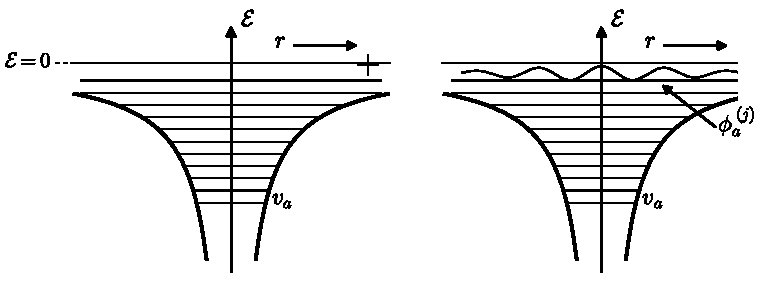
\includegraphics[width=0.72\textwidth]{fig_54.pdf}
\caption*{图 54\quad 自由原子的束缚原子轨道}
\end{figure}

\begin{figure}[H]
\centering
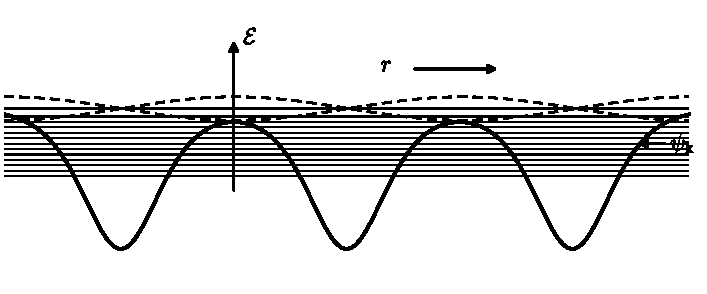
\includegraphics[width=0.72\textwidth]{fig_55.pdf}
\caption*{图 55\quad 晶体的 Bloch 态}
\end{figure}

无论如何，这组函数是\emph{不完备}的，因为它缺少 Schr\"odinger 方程在连续谱中、高于 $v_a(\mathbf{r})$ 能量零点的所有散射波本征态。虽然式 (3.31) 在原子芯内部可以与 $\psi_{\mathbf{k}}$ 匹配得相当好，但它谈不上能表示间隙区域中的 Bloch 态——在那里它必须表现得像自由电子平面波的简单组合（见 §3.6）。

不过，这个方法确实给出了一条重要的形式原理。

在式 (3.26) 中我们看到，$\mathbf{k}$ 空间中的能量可以展开成 Fourier 级数
\begin{equation*}
\mathcal{E}(\mathbf{k})=\sum_{l}e^{i\mathbf{k}\cdot\mathbf{l}}\mathcal{E}_l.
\tag{3.32}
\end{equation*}
可以证明，这种形式的展开总是可能的——也就是说，L.C.A.O. 方法如果精确而彻底地进行下去，将会给出这种形式的能量——尽管系数 $\mathcal{E}_l$ 不再是像式 (3.27) 或 (3.29) 那样的简单积分，而且当 $\mathbf{l}$ 很大时也许收敛得不太快。

现在请记住，正格矢 $\mathbf{l}$ 本身就是倒格子 $\mathbf{g}$ 的倒格矢（§1.3 (iv)）。式 (3.32) 正是如下这类公式
\begin{equation*}
\mathcal{V}(\mathbf{r})=\sum_{\mathbf{g}}e^{i\mathbf{r}\cdot\mathbf{g}}\mathcal{V}_{\mathbf{g}}
\tag{3.33}
\end{equation*}
的对偶（译注：原书此式编号误印为“(3.23)”。）；只要 $\mathcal{V}(\mathbf{r})$ 具有周期性 $\mathcal{V}(\mathbf{r}+\mathbf{l})=\mathcal{V}(\mathbf{r})$，这类公式便成立。于是，\emph{每条能带中的能量函数在倒格子中必须是周期的}；
\begin{equation*}
\mathcal{E}(\mathbf{k}+\mathbf{g})=\mathcal{E}(\mathbf{k}).
\tag{3.34}
\end{equation*}

这个性质我们在上一节中已经注意到。(3.32) 这种表示式有时颇为方便；它使 $\mathcal{E}(\mathbf{k})$ 自动满足这个条件。如果把系数 $\mathcal{E}_l$ 当作可调参数来处理，往往就能用这个公式拟合观测到的费米面。作为内插公式，它的“物理”论证比 N.F.E. 方案略逊一筹——在后一方案中，Fourier 分量 $\mathcal{V}_{\mathbf{g}}$ 可以取作参数——但它更便于计算，因为它把能量直接表示成简单解析函数之和。

\section{元胞法}

L.C.A.O. 方法所受的非议之一，可以通过使用被构造得满足 Bloch 条件 (1.58) 的函数来避免；也就是说，当波函数移动通过晶格平移 $\mathbf{l}$ 时（例如从晶胞的一个面移动到另一个面），它改变一个因子 $\exp(i\mathbf{k}\cdot\mathbf{l})$。另一种做法是，对公式
\begin{equation*}
\psi_{\mathbf{k}}(\mathbf{r})=e^{i\mathbf{k}\cdot\mathbf{r}}u_{\mathbf{k}}(\mathbf{r}),
\tag{3.35}
\end{equation*}
中的函数 $u_{\mathbf{k}}(\mathbf{r})$ 建立微分方程，同时（由式 (1.61)）知道它必须是正格子中的周期函数。

在一维情形，这看上去是个简单的方案。例如，可以选取一个 $\mathcal{E}$ 值，积分方程，看条件是否满足，再改变 $\mathcal{E}$，如此等等。但在三维情形，它是笨拙的。条件 (3.34) 必须在晶胞的整个面上成立——这就意味着要在无穷多个点上成立。于是，人们在晶胞内构造各种球谐函数的解，并寻找在晶胞边界上有限个点处相匹配的线性组合。这还可以改进：在晶胞表面上定义一个平均匹配误差，并通过改变系数使其极小。这一步骤在数学上很繁琐，但原理上足够明了；它曾为某些固体给出过相当好的能带结构，但在新理论概念方面却少有贡献。

元胞法看上去简单而直接。晶胞是一个定义明确的几何概念，Bloch 条件也很容易写下。但是整个想法并不很对头。我们不应当人为地设立晶胞边界，偏偏在势最为平坦、波函数最接近自由电子波函数的区域制造匹配间断。匹配条件只能任意地定义，而有时表面上看去合理的做法竟给出完全错误的结果，甚至连空晶格这种初等情形也不例外。

这种一般性的元胞方法有一个前身，有时颇为有用。这就是 \emph{Wigner--Seitz 方法}。我们注意到，F.C.C. 或 B.C.C. 格子的晶胞——即 Wigner--Seitz 原胞——是一个近似于球体的规则多面体。姑且假定它是一个球，体积与晶胞相同，即半径为 $r_s$（参看式 (2.54)）。

考虑 $\mathbf{k}=0$ 的态。它必须满足
\begin{equation*}
\psi_{\mathbf{k}}(\mathbf{r}+\mathbf{l})=\psi_{\mathbf{k}}(\mathbf{r});
\tag{3.36}
\end{equation*}
即它必须逐个晶胞地周期。这意味着它在晶胞边界上应当有水平切线；我们可以说它必须满足条件
\begin{equation*}
\left.\frac{\partial\psi_{\mathbf{k}}}{\partial r}\right]_{r=r_s}=0
\tag{3.37}
\end{equation*}
于 Wigner--Seitz 球面上。这样一来，如果势在球内是球对称的，我们只需在这个边界条件下求解一个径向方程，于是能量 $\mathcal{E}(0)$ 便可唯一地确定（图 56）。

\begin{figure}[H]
\centering
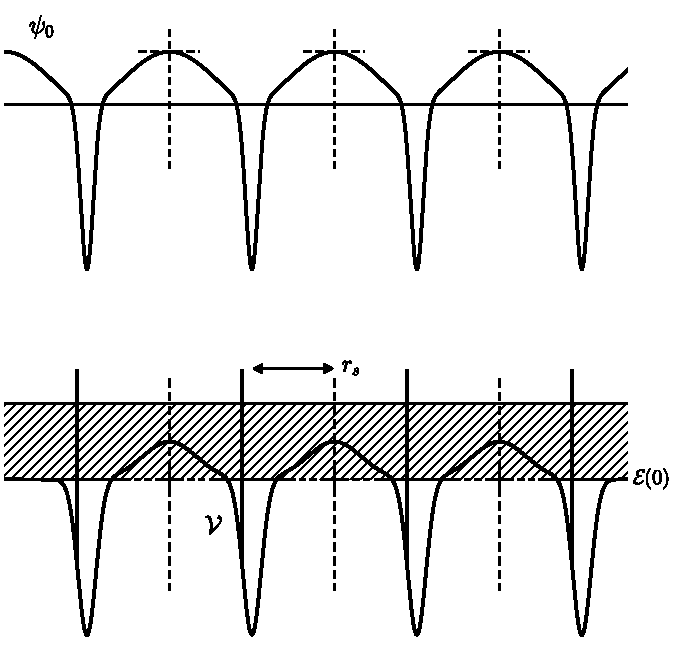
\includegraphics[width=0.72\textwidth]{fig_56.pdf}
\caption*{图 56\quad Wigner--Seitz 方法}
\end{figure}

这是确定单价金属导带底位置的一个巧妙办法，在计算金属内聚能（§4.3）时可以相当有把握地使用它。我们还可以再前进一步，写下方程
\begin{equation*}
-\frac{\hbar^2}{2m}\left\{\nabla^2+2i\mathbf{k}\cdot\nabla\right\}u_{\mathbf{k}}+\mathcal{V}(\mathbf{r})\,u_{\mathbf{k}}
=\left\{\mathcal{E}(\mathbf{k})-\frac{\hbar^2 k^2}{2m}\right\}u_{\mathbf{k}}\tag{3.38}
\end{equation*}
(3.35) 中的周期函数 $u_{\mathbf{k}}(\mathbf{r})$ 必须满足这个方程；而且我们还可以进而坚持要求 $u_{\mathbf{k}}$ 在 $r=r_s$ 处具有水平切线。这样一来，从 $\mathcal{E}(0)$ 量起的函数 $\mathcal{E}(\mathbf{k})$ 就会给出某种不同于自由电子公式的结果，从而带上几分能带形状的特征。

但在这个方法里，我们完全忽略了固体的结构。答案只依赖于原子体积，而不依赖于晶格的实际几何构形。对于液体——其中每个原子的环境是无序的——我们应当得到与同样密度的固态金属完全相同的结果；那些我们在前面几节里不厌其详地讨论过的美丽衍射效应，在这里根本就进不来。

\section{正交化平面波}

现在我们转向几种真正行之有效的能带结构计算方法。例如，紧束缚法（§3.4）受到的那些根本性诘难，可以通过如下做法来化解：(a) 在原子轨道的 Bloch 和 (3.31) 中有意加入像 (3.12) 那样的平面波项；(b) 从后一个和里剔除所有那些在原子势相互重叠时实际上已经消失的虚构轨道（图 54 和图 55）。Herring 在引入\emph{正交化平面波}（orthogonalized plane wave，OPW）概念时所做的正是这两件事。

考虑一组由\emph{芯态}（core states）——也就是在离子中早已被占据的轨道——构成的 Bloch 函数。由 (3.24) 可以写出
\begin{equation*}
b_{l\mathbf{k}}=\sum_l e^{i\mathbf{k}\cdot\mathbf{l}}\,b_l(\mathbf{r}-\mathbf{l}).\tag{3.39}
\end{equation*}
像 $b_l(\mathbf{r})$ 这样的一个芯轨道是高度局域化的，因此上式不过是简并单电子态的一种组合，其中每一个态对应于电子局域在一个特定原子上。实际上，它是整个晶体的 Schrödinger 方程的解，对应于某一芯能级 $\mathcal{E}_l$。它可以形成一条窄带，在晶体中这条带是全满的。

较高的那些态既然是同一个 Schrödinger 方程的解，就\emph{必须与} $b_{l\mathbf{k}}$ \emph{正交}：
\begin{equation*}
\langle\psi_{\mathbf{k}},b_{l\mathbf{k}}\rangle=0.\tag{3.40}
\end{equation*}
此外我们知道，在原子之间的区域，$\psi_{\mathbf{k}}$ 必须看起来像一列自由电子波。让我们试着取
\begin{equation*}
\chi_{\mathbf{k}}=e^{i\mathbf{k}\cdot\mathbf{r}}-\sum_l\beta_l\,b_{l\mathbf{k}}\tag{3.41}
\end{equation*}
作为其中一个较高态的波函数的一种可能形式。只要适当选取系数 $\beta_l$，就能使它满足正交化条件 (3.40)。也就是说，我们把 $\chi_{\mathbf{k}}$ 做成一个\emph{正交化平面波}（O.P.W.）
\begin{equation*}
\chi_{\mathbf{k}}=e^{i\mathbf{k}\cdot\mathbf{r}}-\sum_l\langle b_{l\mathbf{k}},e^{i\mathbf{k}\cdot\mathbf{r}}\rangle\,b_{l\mathbf{k}}.\tag{3.42}
\end{equation*}

对于较高的态，这是一个很好的猜测：在间隙区域里它看起来像 $\exp(i\mathbf{k}\cdot\mathbf{r})$——那里每个 $b_{l\mathbf{k}}$ 都很小（芯态高度局域化）——而在芯区内部，它又与所有芯态正交，因而是较高原子轨道的一个不错的候选者。举例来说，设芯态是 $2s$ 和 $2p$，各有一个节面：于是 $\chi_{\mathbf{k}}$ 将多出一个节面，正像 $3s$ 或 $3p$ 轨道那样。

现在我们用 O.P.W. 作为波函数的基态，尝试
\begin{equation*}
\psi_{\mathbf{k}}=\sum_{\mathbf{g}}\alpha_{\mathbf{k}-\mathbf{g}}\,\chi_{\mathbf{k}-\mathbf{g}}\tag{3.43}
\end{equation*}
作为 Schrödinger 方程的解，做法与 (3.12) 相同。我们用变分原理把能量期望值极小化，从而确定系数 $\alpha_{\mathbf{k}-\mathbf{g}}$。这套手续如今已为大家所熟悉，不必再显式写出了。

这种近似过程在初始阶段收敛得惊人地快。单个 O.P.W. 往往就足以在 k 空间的大片区域上代表波函数；取 3 项或 4 项便能给出相当好的图像，甚至到布里渊区最偏远的角落也不例外。这个方法已经成功地用于若干金属和半导体，而且并不局限于“被空白区域包围的球对称势”这种情形。

为什么会这样？下面这个归功于 Phillips 和 Kleinman 的论证非常有说服力。

假定 (3.43) 在 $\alpha_{\mathbf{k}-\mathbf{g}}$ 取某组确定值时就是严格的波函数。写下函数
\begin{equation*}
\phi=\sum_{\mathbf{g}}\alpha_{\mathbf{k}-\mathbf{g}}\,e^{i(\mathbf{k}-\mathbf{g})\cdot\mathbf{r}},\tag{3.44}
\end{equation*}
\begin{figure}[H]
\centering
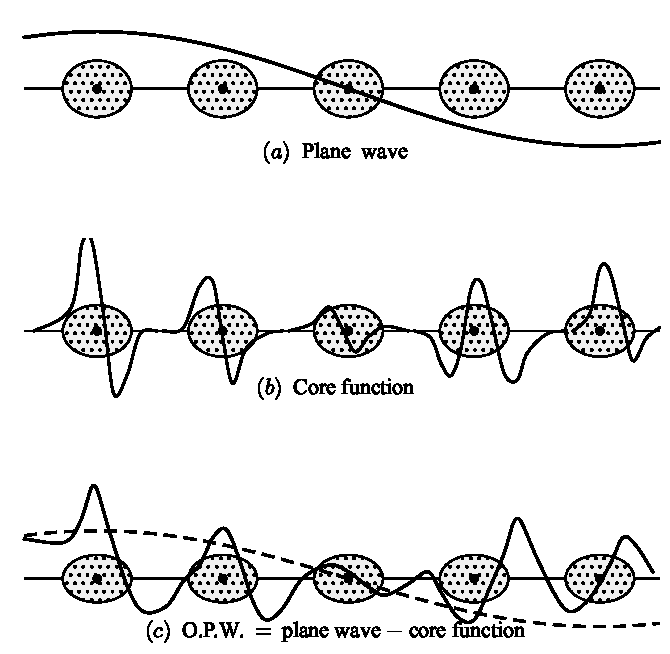
\includegraphics[width=0.72\textwidth]{fig_57.pdf}
\caption*{图 57\quad 正交化平面波的合成。(a)平面波；(b)芯函数；(c)O.P.W.＝平面波－芯函数}
\end{figure}
——即由简单平面波按同样的系数组合而成的函数。于是 (3.42) 与 (3.43) 可以写成（略去指标 $\mathbf{k}$，它自始至终不变）
\begin{equation*}
\psi=\phi-\sum_l\langle b_l,\phi\rangle\,b_l.\tag{3.45}
\end{equation*}
把它代入 Schrödinger 方程 $\mathcal{H}\psi=\mathcal{E}\psi$，即
\begin{equation*}
\mathcal{H}\phi-\sum_l\langle b_l,\phi\rangle\,\mathcal{H}b_l=\mathcal{E}\phi-\mathcal{E}\sum_l\langle b_l,\phi\rangle\,b_l,\tag{3.46}
\end{equation*}
亦即
\begin{equation*}
\mathcal{H}\phi-\sum_l\langle b_l,\phi\rangle\,\mathcal{E}_l b_l+\mathcal{E}\sum_l\langle b_l,\phi\rangle\,b_l=\mathcal{E}\phi,\tag{3.47}
\end{equation*}
这里用到 $b_l$ 也是 $\mathcal{H}$ 的本征态、其能量为 $\mathcal{E}_l$ 这一事实。于是
\begin{equation*}
\mathcal{H}\phi+\sum_l(\mathcal{E}-\mathcal{E}_l)\,b_l\langle b_l,\phi\rangle=\mathcal{E}\phi.\tag{3.48}
\end{equation*}

我们可以把它看成一个新的 Schrödinger 方程
\begin{equation*}
(\mathcal{H}+\mathcal{V}_R)\phi=\mathcal{E}\phi,\tag{3.49}
\end{equation*}
式中我们对一个算符作如下形式定义：
\begin{equation*}
\mathcal{V}_R\phi\equiv\sum_l(\mathcal{E}-\mathcal{E}_l)\,b_l\langle b_l,\phi\rangle.\tag{3.50}
\end{equation*}
我们的“平滑化”波函数 $\phi$ 现在满足一个新方程，其“哈密顿量”是
\begin{equation*}
\mathcal{H}+\mathcal{V}_R=-\frac{\hbar^2}{2m}\nabla^2+\mathcal{V}+\mathcal{V}_R.\tag{3.51}
\end{equation*}
这就好比我们要在一个\emph{赝势}（pseudo-potential）
\begin{equation*}
\Gamma=\mathcal{V}+\mathcal{V}_R.\tag{3.52}
\end{equation*}
中求本征函数的平面波解。

§3.2 的那套形式手续现在可以拿来使用了。系数 $\alpha_{\mathbf{k}-\mathbf{g}}$ 必须满足与 (3.14) 相仿的方程，只不过其中要用 $\Gamma$ 的 Fourier 分量来代替真实晶格势 $\mathcal{V}$ 的 Fourier 分量。

当然，这些方程只是把 (3.43) 取作试探波函数、对能量期望值中的系数 $\alpha_{\mathbf{k}-\mathbf{g}}$ 作变分所得方程的另一种写法。但结果表明（这一点可以上升为一条普遍原理来论证）：除了头几个倒格矢之外，$\Gamma$ 的 Fourier 分量都很小。函数 $\phi$ 可以称为\emph{赝波函数}（pseudo-wave-function），它所满足的方程 (3.49) 中的有效势相对较弱。这样我们又回到了一个简单的 N.F.E. 模型。

把 $\Gamma$ 当作一个小的局域势来处理，这个论证并不严格。符号 $\mathcal{V}_R$ 代表的是一个非局域算符
\begin{equation*}
\mathcal{V}_R(\mathbf{r},\mathbf{r}')=\sum_l(\mathcal{E}-\mathcal{E}_l)\,b_l(\mathbf{r})\,b_l^{*}(\mathbf{r}'),\tag{3.53}
\end{equation*}
它通过下式起作用：
\begin{equation*}
\mathcal{V}_R\phi=\int\mathcal{V}_R(\mathbf{r},\mathbf{r}')\,\phi(\mathbf{r}')\,d\mathbf{r}'.\tag{3.54}
\end{equation*}
这告诉我们，比如说，$\mathcal{V}_R$ 作用在不同角动量的函数上时必定有所不同；我们应当写成
\begin{equation*}
\mathcal{V}_R=\mathcal{V}_s+\mathcal{V}_p+\mathcal{V}_d+\dots,\tag{3.55}
\end{equation*}
其中 $\mathcal{V}_s$ 只作用在具有 $s$ 对称性的函数上，如此等等。

问题的实质在于：$\mathcal{V}$ 是原子的吸引势，因而是负的，尤其在 $r=0$ 附近更是如此；而 $\mathcal{V}_R$ 含有 $\mathcal{E}-\mathcal{E}_l$ 和芯轨道的平方，因而是正的。两者之间有部分抵消，使 $\mathcal{V}_{\mathrm{eff}}$ 的数值减小。这种抵消虽然永远不会完全，但可以通过适当选取芯函数而得到改善。
实际上，构造 $\mathcal{V}_R$ 的整个过程并不是唯一的。可以证明：\emph{哈密顿量 $(\mathcal{H}+\mathcal{V}_R)$ 的价电子本征值，对于任何形如下式的算符都是相同的}
\begin{equation*}
\mathcal{V}_R\phi=\sum_l\langle F_l,\phi\rangle\,b_l,\tag{3.56}
\end{equation*}
\emph{其中诸 $F_l$ 是完全任意的函数}。要看出这一点，请注意算符 $\mathcal{V}_R$ 总是把 $\phi$ 投影到芯态所张的流形上，而我们正在寻找的价电子本征函数与这个流形正交——因此，把算符 $\mathcal{V}_R$ 加到哈密顿量上，对价电子本征函数空间中的本征值问题毫无影响。

于是，只要明智地选取函数 $F_l$，我们就可以设法获得良好的抵消。例如，若取
\begin{equation*}
F_l=-\mathcal{V}b_l,\tag{3.57}
\end{equation*}
便得到
\begin{equation*}
\Gamma\phi=\mathcal{V}\phi-\sum_l\langle b_l,\mathcal{V}\phi\rangle\,b_l,\tag{3.58}
\end{equation*}
这表明我们可以从 $\mathcal{V}$ 中减去任何能展开成芯函数之和的部分。这就解释了为什么在许多情况下 $\Gamma$ 结果相当小。

这样，抵消原理虽然不是一个严格的定理，却为\emph{赝势概念}提供了依据：\emph{金属和半导体中的价电子，其行为就好像它们与晶格的离子并没有强烈的相互作用一样}。这就是 §3.3 的 N.F.E. 模型在经验上取得成功的原因——不仅在于它给出了费米面的漂亮图像（如图 49），也在于它能处理复杂得多的现象，例如电阻率和声子谱的理论（参见 §§6.12、6.13）。无论从哪方面看，这都是自 1930 年代初 Bloch 的工作以来固体理论中最富成果的进展之一。

然而，从理论的角度看，这种基于 O.P.W. 形式体系的“解析”赝势并不完全令人满意：它过于强烈地依赖能量和角动量；它不是真正的局域势；它的定义不唯一；它也无法优雅地处理 $d$ 带（见 §3.10）。它所确立的要点——N.F.E. 模型远比乍看之下的样子要好——几乎同样可以从下一节要讨论的“muffin-tin”方法得到，而无须引入像 (3.44) 中函数 $\phi$ 那样的赝平面波（Ψ.P.W.）。

\section{增广平面波}

L.C.A.O. 方法和元胞法之所以受到诘难，是由于金属中的势在离子实之间相当平坦。我们索性假定它是一个 \emph{muffin-tin 势}（muffin-tin potential，蛋盒势）——在每个格点周围半径 $R_s$ 以内球对称，而在间隙区域为常数。再假定 $R_s$ 小于 Wigner--Seitz 半径 $r_s$，使这些球互不相交。于是，在每个球内部我们都可以用球谐函数把 Schrödinger 方程严格解出，
\begin{figure}[H]
\centering
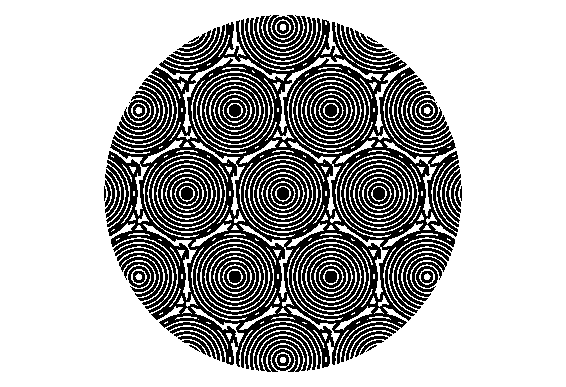
\includegraphics[width=0.72\textwidth]{fig_58.pdf}
\caption*{图 58\quad muffin-tin 势}
\end{figure}
而在球与球之间的体积中我们也能求出严格解——平面波。只要在每个球面上把这些解匹配起来，就能构造出遍及整个晶体的 Schrödinger 方程的解。

实际的做法如下：设 $\mathcal{E}$ 是我们这个态的能量。在每个球内部，Schrödinger 方程的解具有如下形式：
\begin{equation*}
\phi(\mathbf{r})=\sum_{lm}C_{lm}\,\mathcal{R}_l(r,\mathcal{E})\,Y_{lm}(\theta,\phi),\tag{3.59}
\end{equation*}
其中 $Y_{lm}(\theta,\phi)$ 是对应于矢量 $\mathbf{r}$ 的方向 $(\theta,\phi)$ 的球谐函数，而 $\mathcal{R}_l$ 是径向方程（采用原子单位）
\begin{equation*}
-\frac{1}{r^2}\frac{\partial}{\partial r}\left(r^2\frac{\partial\mathcal{R}_l}{\partial r}\right)+\left\{\frac{l(l+1)}{r^2}+\mathcal{V}(r)\right\}\mathcal{R}_l=\mathcal{E}\,\mathcal{R}_l\tag{3.60}
\end{equation*}
的解。

现在我们来选取系数 $C_{lm}$，使得 $\phi(\mathbf{r})$ 在球面 $r=R_s$ 上恰好与单一平面波 $\exp(i\mathbf{k}\cdot\mathbf{r})$ 相匹配。利用平面波按球谐函数展开的标准公式，容易证明，只要取
\begin{equation*}
C_{lm}=(2l+1)\,i^{\,l}\left\{j_l(kR_s)\big/\mathcal{R}_l(R_s,\mathcal{E})\right\}Y_{lm}^{*}(\theta',\phi')\tag{3.61}
\end{equation*}
即可做到这一点，其中 $\theta'$、$\phi'$ 给出 $\mathbf{k}$ 的方向，$j_l$ 是球 Bessel 函数。把 (3.61) 代入 (3.59)，我们就定义了一个\emph{增广平面波}（augmented plane wave，A.P.W.）$\phi_{\mathbf{k}}(\mathbf{r})$，它在间隙区域中等于 $\exp(i\mathbf{k}\cdot\mathbf{r})$，而在以 $\mathbf{l}$ 为中心的球内则满足
\begin{equation*}
\phi_{\mathbf{k}}(\mathbf{r})=e^{i\mathbf{k}\cdot\mathbf{l}}\,\phi_{\mathbf{k}}(\mathbf{r}-\mathbf{l})\tag{3.62}
\end{equation*}

遗憾的是，就整个晶格的势而言，这个函数仍然不是我们 Schrödinger 方程的解。的确，我们并没有对能量 $\mathcal{E}$ 与波矢 $\mathbf{k}$ 之间的关系作任何特别的假定。但我们知道，最终的波函数可以由 A.P.W. 构造出来——而且根据 Bloch 定理，它必定取如下形式
\begin{equation*}
\psi_{\mathbf{k}}(\mathbf{r})=\sum_{\mathbf{g}}\alpha_{\mathbf{k}-\mathbf{g}}\,\phi_{\mathbf{k}-\mathbf{g}}(\mathbf{r}),\tag{3.63}
\end{equation*}
其中系数 $\alpha_{\mathbf{k}-\mathbf{g}}$ 有待确定。

下一步是把 (3.63) 用作试探函数，对能量作变分估计。容易证明，这些系数必须满足形如
\begin{equation*}
\left\{(\mathbf{k}-\mathbf{g})^2-\mathcal{E}\right\}\alpha_{\mathbf{k}-\mathbf{g}}+\sum_{\mathbf{g}'}\Gamma_{\mathbf{gg}'}\,\alpha_{\mathbf{k}-\mathbf{g}'}=0,\tag{3.64}
\end{equation*}
的方程，其中 $\Gamma_{\mathbf{gg}'}$ 是一个含有 $\phi_{\mathbf{k}-\mathbf{g}}$、$\phi_{\mathbf{k}-\mathbf{g}'}$ 以及与周期势相联系的哈密顿算符的积分。

这些积分的显式公式，其推导会使我们过于深入方法的细节；结果为
\begin{align*}
\Gamma_{\mathbf{gg}'}=\frac{4\pi R_s^2}{v_c}\Big\{&-\left[(\mathbf{k}-\mathbf{g}')\cdot(\mathbf{k}-\mathbf{g})-\mathcal{E}\right]\frac{j_1\left(|\mathbf{g}-\mathbf{g}'|\,R_s\right)}{|\mathbf{g}-\mathbf{g}'|}\\
&+\sum_{l=0}^{\infty}(2l+1)\,P_l(\cos\theta_{\mathbf{gg}'})\,j_l\left(|\mathbf{k}-\mathbf{g}|\,R_s\right)j_l\left(|\mathbf{k}-\mathbf{g}'|\,R_s\right)\\
&\qquad\qquad\times\frac{\mathcal{R}'_l(R_s,\mathcal{E})}{\mathcal{R}_l(R_s,\mathcal{E})}\Big\}\tag{3.65}
\end{align*}
（其中 $\theta_{\mathbf{gg}'}$ 是 $(\mathbf{k}-\mathbf{g})$ 与 $(\mathbf{k}-\mathbf{g}')$ 之间的夹角，$\mathcal{R}'_l$ 是径向函数 $\mathcal{R}_l$ 的导数）。这一手续的实质，是让球外区域给出一个像 (3.65) 中第一主项那样的贡献；其余部分则来自梯度算符对每个 A.P.W. 在各个球面上的斜率不连续所起的作用。

能带结构问题现在就归结为求线性方程组 (3.64) 的解——只有当久期行列式为零时，解才可能存在。现在假定我们选定一个 $\mathbf{k}$ 值。所有系数都将依赖于 $\mathcal{E}$——或像 (3.64) 中那样显式地依赖，或通过 (3.65) 隐式地依赖。我们可以对给定的 $\mathcal{E}$ 值算出行列式，然后改变 $\mathcal{E}$，直到找出一个根为止。这个 $\mathcal{E}$ 值就是我们对 $\mathcal{E}(\mathbf{k})$ 的估计。

A.P.W. 方法是计算金属能带结构的一种稳妥实用的程序。它需要大量计算，但确实行之有效。例如，结果对原子势半径 $R_s$ 的选取并不十分敏感，而且在存在 $d$ 带时依然适用（见 §3.10）。然而，这里有趣的一点是，兜了一圈之后，我们最终回到了在结构上与 N.F.E. 法相似的那些公式。(3.64) 与式 (3.14) 完全相同，只不过我们用一个更复杂的表达式取代了原子势的 Fourier 分量，即
\begin{equation*}
\mathcal{V}_{\mathbf{g}-\mathbf{g}'}\rightarrow\Gamma_{\mathbf{gg}'}.
\end{equation*}
换言之，$\Gamma_{\mathbf{gg}'}$ 正是某个有效原子势的 Fourier 分量。倘若它碰巧不怎么依赖 $\mathcal{E}$ 和 $\mathbf{k}$，而只是 $|\mathbf{g}-\mathbf{g}'|$ 的函数，那么我们就可以直接用 N.F.E. 方法构造出费米面等等。

遗憾的是，A.P.W. 赝势分量 (3.65) 通常并不像我们希望的那样小。这一点由“空格子检验”（empty lattice test）即可看出：在 $\mathcal{V}(\mathbf{r})\equiv 0$ 的“晶格”中求解 $\mathcal{E}(\mathbf{k})$ 时，(3.65) 中函数 $R_l$ 的径向导数在 $r=R_s$ 处并不自动为零，因此即使真实势的 Fourier 分量 $\mathcal{V}_{\mathbf{g}-\mathbf{g}'}$ 为零，系数 $\Gamma_{\mathbf{gg}'}$ 也不趋于零。这样一来，仅仅为了得到平庸的结果 $\mathcal{E}(\mathbf{k})=k^2$，就得做大量的计算。因此，A.P.W. 方法在实践上的成功，并不能直接求助于 §3.6 的赝势概念来论证。这一点将在 §3.8 中进一步讨论。

\section{Green 函数法}

有一种技术在原理上看起来截然不同，推演出来的结果却颇为相似：它从任意势 $\mathcal{V}(\mathbf{r})$ 中波函数的标准积分方程出发：
\begin{equation*}
\psi(\mathbf{r})=-\frac{1}{4\pi}\int\frac{\exp(i\kappa\,|\mathbf{r}-\mathbf{r}'|)}{|\mathbf{r}-\mathbf{r}'|}\,\mathcal{V}(\mathbf{r}')\,\psi(\mathbf{r}')\,d\mathbf{r}',\tag{3.66}
\end{equation*}
其中
\begin{equation*}
\kappa^2=\mathcal{E}\tag{3.67}
\end{equation*}
因而当 $\mathcal{E}>0$ 时 $\kappa$ 为实数，当 $\mathcal{E}<0$ 时 $\kappa$ 为虚数。

这个方程说的是：波函数被势散射到自身之中，达到自洽；来自各个不同点 $\mathbf{r}'$、强度为 $\mathcal{V}(\mathbf{r}')\psi(\mathbf{r}')$ 的小波，重新合成为 $\psi(\mathbf{r})$。现在假定我们有一个 muffin-tin 势，即
\begin{equation*}
\mathcal{V}(\mathbf{r})=\sum_l v_a(\mathbf{r}-\mathbf{l}).\tag{3.68}
\end{equation*}
代入 (3.66)，得
\begin{equation*}
\psi(\mathbf{r})=-\frac{1}{4\pi}\sum_l\int\frac{\exp(i\kappa\,|\mathbf{r}-\mathbf{r}'|)}{|\mathbf{r}-\mathbf{r}'|}\,v_a(\mathbf{r}'-\mathbf{l})\psi(\mathbf{r}')\,d\mathbf{r}',\tag{3.69}
\end{equation*}
式中积分仅遍及 $\mathbf{l}$ 周围的元胞，因为 $v_a(\mathbf{r}-\mathbf{l})$ 在其他地方为零。

我们要找的是一个 Bloch 函数。利用这一性质，可以把 $\psi(\mathbf{r}')$ 的原点移到 $\mathbf{r}'-\mathbf{l}$ 处，再把它重新记作 $\mathbf{r}''$。于是
\begin{align*}
\psi_{\mathbf{k}}(\mathbf{r})&=-\frac{1}{4\pi}\sum_l\int\frac{\exp(i\kappa\,|\mathbf{r}-\mathbf{r}'|)}{|\mathbf{r}-\mathbf{r}'|}\,v_a(\mathbf{r}'-\mathbf{l})\,e^{i\mathbf{k}\cdot\mathbf{l}}\psi_{\mathbf{k}}(\mathbf{r}'-\mathbf{l})\,d\mathbf{r}'\\
&=-\frac{1}{4\pi}\int\left\{G(\kappa,\mathbf{k};\mathbf{r}-\mathbf{r}'')\right\}v_a(\mathbf{r}'')\psi_{\mathbf{k}}(\mathbf{r}'')\,d\mathbf{r}''.\tag{3.70}
\end{align*}
这实际上就是说，$\mathbf{r}$ 处的波函数是所有其他元胞（位于 $\mathbf{l}$ 等处）散射出的小波各带适当相位因子后的贡献之和。由于所有元胞全同，我们得以引入\emph{结构 Green 函数}（structural Green function），或称 Greenian：
\begin{equation*}
G(\kappa,\mathbf{k};\mathbf{r}-\mathbf{r}'')\equiv\sum_l\frac{\exp(i\kappa\,|\mathbf{r}-\mathbf{r}''+\mathbf{l}|)}{|\mathbf{r}-\mathbf{r}''+\mathbf{l}|}\,e^{i\mathbf{k}\cdot\mathbf{l}},\tag{3.71}
\end{equation*}
它给出从 $\mathbf{r}''$ 以及所有其他元胞中各等价点散射来的波在 $\mathbf{r}$ 处的效果（图 59b）。这样一来，我们只需在单个元胞中积分，便能得出整个波函数。

\begin{figure}[H]
\centering
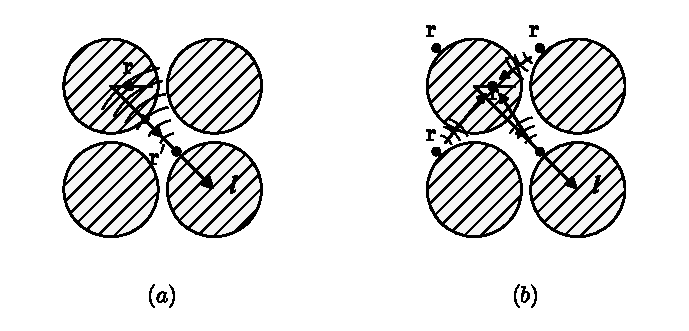
\includegraphics[width=0.72\textwidth]{fig_59.pdf}
\caption*{图 59\quad 普通的 Green 函数（(a)）描述从 $\mathbf{r}'$ 到 $\mathbf{r}$ 的传播；现以结构 Green 函数（(b)）取代之，后者把来自晶格中所有等价点 $\mathbf{r}''$ 的波组合起来}
\end{figure}

论证的下一步是构造一个泛函，使它经变分后给出积分方程 (3.70)。容易证明，这个泛函就是
\begin{align*}
\Lambda&=N\int\psi_{\mathbf{k}}^{*}(\mathbf{r})\,v_a(\mathbf{r})\,\psi_{\mathbf{k}}(\mathbf{r})\,d\mathbf{r}\\
&\quad+\frac{1}{4\pi}\iint\psi_{\mathbf{k}}^{*}(\mathbf{r})\,v_a(\mathbf{r})\,G(\kappa,\mathbf{k};\mathbf{r}-\mathbf{r}'')\,v_a(\mathbf{r}'')\psi_{\mathbf{k}}(\mathbf{r}'')\,d\mathbf{r}\,d\mathbf{r}''.\tag{3.72}
\end{align*}
积分只需遍及单个元胞——而且由于势在每个原子球以外处处为零，每重积分都可以限制在 $r,r''\leqslant R_s$ 的范围内。

现在我们在每个元胞内部假设一个与 (3.59) 同形的试探波函数
\begin{equation*}
\psi_{\mathbf{k}}(\mathbf{r})=\sum_{lm}C_{lm}\,\mathcal{R}_l(r)\,Y_{lm}(\theta,\phi).\tag{3.73}
\end{equation*}
显然，(3.72) 最终将成为系数 $C_{lm}$ 的一个二次函数
\begin{equation*}
\Lambda=\sum_{lm;\,l'm'}\Lambda_{lm;l'm'}\,C_{lm}\,C_{l'm'}^{*}\tag{3.74}
\end{equation*}
变分条件给出一组线性方程，其行列式 $|\Lambda_{lm;l'm'}|$ 必须为零。这个行列式是波矢 $\mathbf{k}$ 和能量 $\mathcal{E}=\kappa^2$ 的函数。行列式的根给出 $\mathcal{E}(\mathbf{k})$ 各支所要求的关系。

这个行列式的具体形式颇有意思。它的各项为
\begin{equation*}
\Lambda_{lm;l'm'}=A_{lm;l'm'}+\kappa\,\delta_{ll'}\,\delta_{mm'}\,\frac{n'_l-n_l L_l}{j'_l-j_l L_l}.\tag{3.75}
\end{equation*}
系数 $A_{lm;l'm'}$ 就其起源而言是结构性的。它们来自
Green 函数 (3.71) 沿 $\mathbf{r}$ 和 $\mathbf{r}''$ 方向的球谐函数展开。这些系数依赖于 $\kappa$ 和 $\mathbf{k}$——但除此之外只依赖于晶格结构。实际公式非常复杂，因为其中要涉及各种宗量的 Clebsch–Gordan 系数以及球 Bessel 函数 $j_l$ 和 $n_l$。要计算晶格和，Ewald 方法（§2.3）也很有用（从分母的形式便可以猜到这一点）。不过，一旦针对给定结构编成了数表，系数 $A_{lm;l'm'}$ 就不必再重新计算。

原子势是通过径向函数 $\mathcal{R}_l$ 在球面上的对数导数 $L_l$ 进来的——正如 (3.66) 中那样。之所以如此，是因为尝试函数 (3.73) 在原子球内部满足 Schrödinger 方程，于是我们可以在 (3.70) 与 (3.72) 的被积函数中写出
\begin{equation*}
v_a(\mathbf{r})\,\psi_{\mathbf{k}}(\mathbf{r})=\left(\nabla^2+\mathcal{E}\right)\psi_{\mathbf{k}}(\mathbf{r})\tag{3.76}
\end{equation*}
随后使用 Green 定理，便得到一个面积分，其中出现 Green 函数的导数（它们在 (3.75) 中表现为 $n_l$ 与 $j_l$）以及径向函数的导数。在这个方法中，假定每个原子的 muffin-tin 势是球对称的，这一点至关重要。

由以上讨论可以清楚地看到，Green 函数方法（也称为 Korringa、Kohn 与 Rostoker 方法，即 KKR 方法）与 A.P.W. 方法非常相似。在 A.P.W. 方法中，我们按需要把展开做到任意多的球谐函数项，然后要求解一个久期行列式，以求出来自不同倒格矢的贡献。在 KKR 方法中，我们对格矢求和（实际上，经过对 $G(\kappa,\mathbf{k};\mathbf{r}-\mathbf{r}'')$ 作 Fourier 变换，是对倒格矢求和），但得到的久期行列式是按不同球谐函数的贡献写出的。两种方法都需要高速计算机，而且两者都工作得相当好。KKR 方法的优点是：结构性质与原子性质在行列式的各项中是分离开的，因此可以分别计算、快速合并。A.P.W. 的优点则是：它对原子球以外的波函数给出更好的图像。

\section{模型赝势}

我们在 §3.6 中已经看到，每个原子势对电子的作用，看起来不过是一个弱赝势（pseudo-potential）的作用。这个重要原理，如何体现在基于 muffin-tin 点阵的能带结构技术之中呢？

原子势并不显式地出现在 A.P.W. 和 KKR 公式 (3.65) 与 (3.75) 之中——它们只依赖于 $\mathcal{R}_l$ 在原子球面上的梯度。这个量同样出现在球形势散射的分波理论（partial wave theory）中（见 §5.5）。我们把每个径向解 $\mathcal{R}_l(r,\mathcal{E})$ 与同能量 $\mathcal{E}=\kappa^2$、同角动量 $l$ 的自由电子波匹配起来，从而定义一个\emph{相移}（phase shift）$\eta_l(\mathcal{E})$，它通过下列公式与 $\mathcal{R}_l$ 的对数导数相联系：
\begin{equation*}
L_l\equiv\frac{\mathcal{R}'_l(R_s,\mathcal{E})}{\mathcal{R}_l(R_s,\mathcal{E})}=\left.\frac{j'_l(\kappa r)-\tan\eta_l(\mathcal{E})\cdot n'_l(\kappa r)}{j_l(\kappa r)-\tan\eta_l(\mathcal{E})\cdot n_l(\kappa r)}\right|_{r=R_s}.\tag{3.77}
\end{equation*}
球 Bessel 函数 $j_l$ 与 $n_l$（连同其导数 $j'_l$ 与 $n'_l$）当然正是径向 Schrödinger 方程 (3.60) 在 muffin-tin 势阱之外的自由空间解。

知道了所有分波在所有能量下的相移，我们便得到了关于原子势所需的全部信息；例如在 (3.75) 中，久期行列式的对角元就只含 $\kappa\cot\eta_l(\mathcal{E})$。这十分自然；相移还给出每个原子的散射截面，从而给出晶格对该能量电子的衍射图样。我们可以预期每个原子的行为，就好像它有一个 $t$ 矩阵即\emph{散射振幅}（scattering amplitude），对沿 $\theta$ 角的散射，取标准的分波形式
\begin{equation*}
t_a(\theta)=-\left(\frac{4\pi N}{\kappa}\right)\sum_l(2l+1)\sin\eta_l\exp(i\eta_l)\,P_l(\cos\theta).\tag{3.78}
\end{equation*}
一个很深的势当然可能产生很大的相移——但在 (3.77) 与 (3.78) 中，我们显然可以忽略每个 $\eta_l$ 中 $\pi$ 的所有整数倍。起作用的只是其余部分——而这个余项可以令散射变得非常弱。在分波理论中，当势阱加深时，截面 $|t_a(\theta)|^2$ 并不会急剧增大；随着束缚态的引入它只是起伏波动，很少大于几个电子波长。换言之，Born 近似——其中从 $\mathbf{k}$ 散射到 $\mathbf{k}'$ 的截面正比于 $|\langle\mathbf{k}'|v_a|\mathbf{k}\rangle|^2$——当 $v_a(\mathbf{r})$ 是一个非常深的势时并不成立。这时我们必须用分波公式 (3.78) 取代势的矩阵元。

这正是 §3.2 的简单 N.F.E. 纲要不收敛的原因。我们是在用微扰论去描述晶体中每个原子的散射。但是，为描写波函数在原子内部快速振荡所需要的高阶 Fourier 系数，与芯区之外 Bloch 态的总体衍射图样基本无关。$\mathcal{R}_l$ 的每个节点都给 $\eta_l$ 增加 $\pi$，但对 (3.65)、(3.75) 或 (3.78) 几乎没有影响。因此，O.P.W. 赝势 (3.50) 正是一个解析手段：通过减去正交化的芯态来消去这些内部节点。剩下的弱赝势 $\Gamma$ 只是一个算符，其矩阵元在原子芯之外给出的波函数，与原来的原子势 $v_a$ 所给出的基本相同。

\begin{figure}[H]
\centering
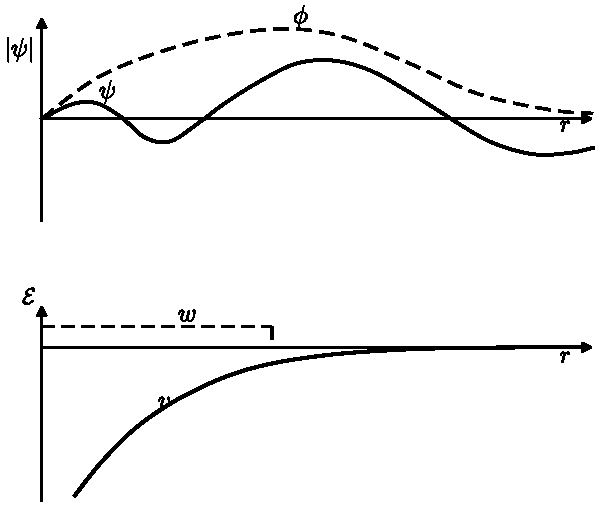
\includegraphics[width=0.72\textwidth]{fig_60.pdf}
\caption*{图 60\quad 模型势 $w$ 连同原子内部的波函数 $\phi$，重现了真实势 $v$ 连同真实波函数 $\psi$ 的效果。}
\end{figure}

对赝势概念的这种诠释，为整个能带结构问题提示了一条替代路线：\emph{把每个原子势 $v_a$ 换成一个弱势 $w_a$，它对传导电子具有相同的散射振幅。}直觉上很清楚，原来晶体中的 $\mathcal{E}(\mathbf{k})$ 将与这个假想材料中的能带结构完全相同，而在后者中 N.F.E. 形式体系如今应当是收敛的。我们所要做的，只是把 (3.14) 中的 $\mathcal{V}_{\mathbf{g}'-\mathbf{g}}$，或
(3.64) 中的 $\Gamma_{\mathbf{gg}'}$，换成我们的\emph{模型势}（model potential）$w_a$ 的相应 Fourier 分量。

这一方案会遇到非局域性、能量依赖性和任意性等困难——这些困难在 (3.56) 那类解析赝势中就已被发现。对给定的能量 $\mathcal{E}$ 和角动量 $l$，存在无穷多个局域势 $w_l(\mathbf{r},\mathcal{E})$，在其中求解径向 Schrödinger 方程 (3.60)，都能在原子芯之外精确重现真实的径向函数 $\mathcal{R}_l$。但同一个模型势通常不能同时适用于不同的 $l$ 值或不同的能量，因此我们必须引入一些算符，把波函数中各个角动量分量分离出来，正如 (3.55) 中那样。实践中，\emph{模型赝势}（model pseudo-potential）中每个 $w_l(\mathbf{r},\mathcal{E})$ 的函数形式，与其说是出于深刻的解析理由，不如说主要是为了计算上的方便。

\begin{figure}[H]
\centering
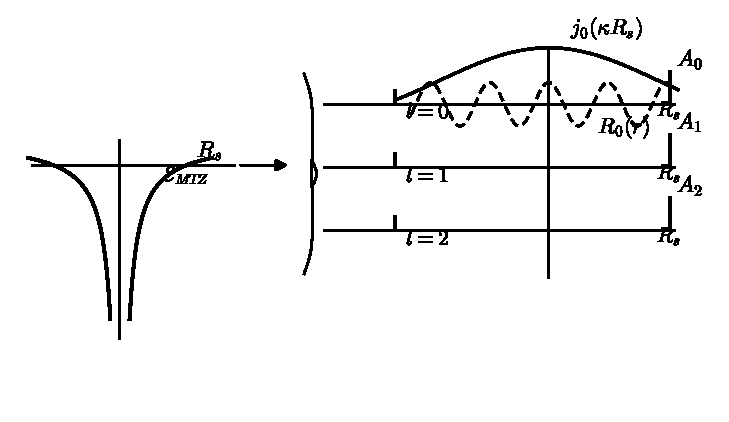
\includegraphics[width=0.72\textwidth]{fig_61.pdf}
\caption*{图 61\quad 用于 KKR 矩阵元的模型赝势。}
\end{figure}

在 muffin-tin 点阵中，一个显然的选择是在原子球面上放一个 $\delta$ 函数奇点，对每个 $l$ 值取适当的强度，使之重现散射相移 $\eta_l(\mathcal{E})$（图 61）。利用平面波和球 Bessel 函数的标准解析性质，我们得到如下形式的“赝势”矩阵元：
\begin{equation*}
\Gamma^{\mathrm{KKR}}_{\mathbf{gg}'}=-\frac{4\pi N}{\kappa}\sum_l(2l+1)\tan\eta'_l\,\frac{j_l(|\mathbf{k}-\mathbf{g}|R_s)\,j_l(|\mathbf{k}-\mathbf{g}'|R_s)}{\left\{j_l(\kappa R_s)\right\}^2}\,P_l(\cos\theta_{\mathbf{gg}'}),\tag{3.79}
\end{equation*}
其中
\begin{equation*}
\cot\eta'_l\equiv\cot\eta_l-n_l(\kappa R_s)\big/j_l(\kappa R_s).\tag{3.80}
\end{equation*}
这个公式与 (3.78)——单个孤立原子的散射振幅——十分相似；在区边界附近，当 $|\mathbf{k}-\mathbf{g}|\sim|\mathbf{k}-\mathbf{g}'|\sim\kappa$ 时，在小相移极限下它便趋于后者。

说来也怪，带这些矩阵元的一组 N.F.E. 方程，其实可以从 KKR 方程的久期行列式出发，经过一连串矩阵变换，从角动量表象 (3.64) 变换到倒格子表象而得到。这个公式与 A.P.W. 矩阵元 (3.65) 之间也有代数上的联系——而后者本身是不能从一组简单的局域势导出的。

实践中，对一个给定晶体计算 muffin-tin 势的分布是相当复杂的过程，屏蔽、关联和交换效应在其中起着重要作用（见第 5 章）。非常方便的做法是：在最初阶段——可以说，在把原子聚拢来构成晶格之前——就把每个原子芯内的深势替换为一个模型赝势 $w$。如果让这个赝势在芯外的行为如同价电子所看到的 Coulomb 函数 $-Ze^2/r$，我们甚至可以计算自由原子的光谱能级，并调整 $w$ 的参数去拟合观测值。这一步骤绕开了自洽原子势等许多理论计算，它就是图 62 中勾画的 Heine–Abarenkov 赝势和 Shaw 赝势的基础。在 $w^{\mathrm{HA}}$ 中，‘芯’的内部（半径可任意选取）被做成平坦的，但可以升高或降低，以便对每个角动量都给出正确的电子本征态；在 $w^{\mathrm{S}}$ 中，则为每个 $l$ 值选取一个半径 $R_l$，使得势在‘芯的边缘’处没有急剧的不连续。然而，困难在于要在 Bloch 态的能量 $\mathcal{E}$ 处选取这些参数，而这个能量未必落在光谱能级的集合之内。

\begin{figure}[H]
\centering
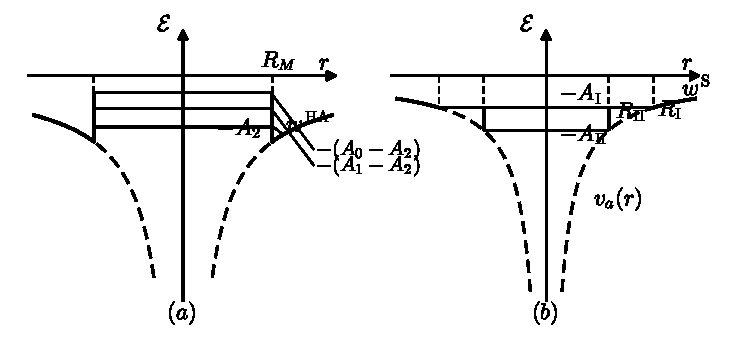
\includegraphics[width=0.72\textwidth]{fig_62.pdf}
\caption*{图 62\quad 模型赝势：(a) Heine–Abarenkov 模型；(b) Shaw 模型。}
\end{figure}

\section{共振能带}

在紧束缚法（§3.4）的早期应用中，人们注意到 $d$ 轨道如此紧缩在原子芯内部，以至于只通过与近邻的重叠产生很窄的带。在\emph{过渡元素}（transition elements）中，这些内层 $d$ 态并未全部填满，而且离 $s$ 或 $p$ ‘价’态非常近——后者本身组合成一条普通的导带。狭窄的‘d 带’的态密度足以容纳每原子至多 10 个电子，它位于‘s-p 带’之内，并在两者相交处与之\emph{杂化}（hybridize）（图 63）。这种情形当然非常重要，因为伴随着磁性现象。

\begin{figure}[H]
\centering
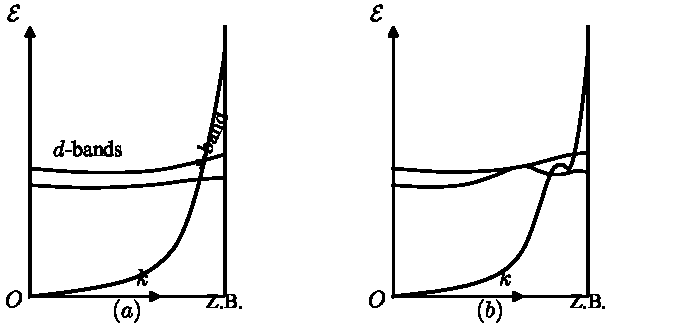
\includegraphics[width=0.72\textwidth]{fig_63.pdf}
\caption*{图 63\quad (a) $d$ 带穿过 $s$ 带；(b) $s$–$d$ 杂化。}
\end{figure}

建立一种内插方案，或者说带可调参数的\emph{模型哈密顿量}（model Hamiltonian），并不困难：其中 $d$ 带用一个 L.C.A.O. 表达式（如 (3.31)）配上适当的赝势分量的矩阵来表示。杂化的程度则由进一步添加的、连接这两个子矩阵的任意矩阵元来确定。

但是，一个像样的定量分析必须顾及 §3.4 中强调的那一点（见图 54）：在我们构成晶体的过程中，原子轨道本身会因势的重叠而被破坏。然而这种破坏并不总是彻底的；在原来 $d$ 轨道的能量附近，仍然可能观察到\emph{虚束缚态}（virtual bound states）。在晶格动力学理论（§2.12）中，我们提到过\emph{共振}（resonance）——一种强烈集中于杂质附近、但在整个晶体中都具有有限振幅的激发。

类似地，电子波函数在共振能量处可以在 muffin-tin 势阱内具有很大的振幅，却并不严格地局域于其中。考察径向 Schrödinger 方程 (3.60) 可知，当 $l\neq0$ 时这种情况很容易发生：‘离心势’ $l(l+1)/r^2$ 提供了一道势垒，电子可以从它的虚态穿过这道势垒隧穿而出（图 64）。

\begin{figure}[H]
\centering
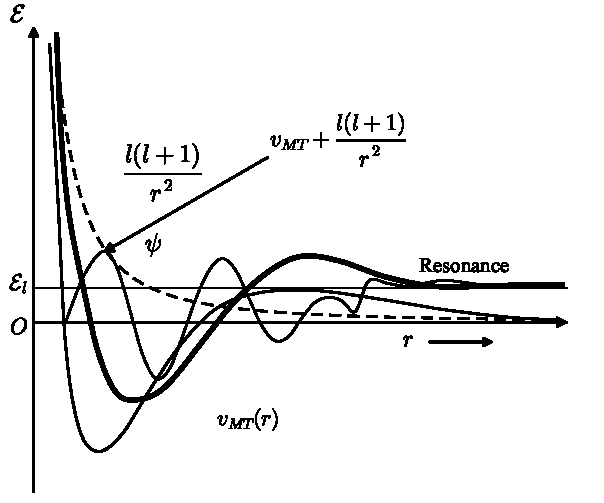
\includegraphics[width=0.72\textwidth]{fig_64.pdf}
\caption*{图 64\quad 虚态波函数穿透离心势垒的隧穿。}
\end{figure}

这类共振的存在——不仅来自 $d$ 态，有时甚至来自自由原子的 $p$ 态——是 §3.6 解析赝势形式体系的隐患之一。例如，我们是否应当把这样的态当作‘芯’的一部分来进行正交化，就不清楚。要理解这一局面，必须再一次转向一般散射理论——共振在那里是人们熟悉的现象。在共振能量 $\mathcal{E}_l$ 附近，第 $l$ 个分波的相移按如下公式经过 $\pi/2$：
\begin{equation*}
\tan\eta_l(\mathcal{E})\approx\frac{W_l}{\mathcal{E}-\mathcal{E}_l}.\tag{3.81}
\end{equation*}
把这个公式塞进比如 A.P.W. 或 KKR 程序里，我们只管摇动手柄，就能得到一个能带结构。其结果是在 $\mathcal{E}(\mathbf{k})$ 中产生以 $\mathcal{E}_l$ 为中心的复杂结构，正如紧束缚图像中那样（图 63）。但是，这条\emph{共振能带}（resonance band）在导带中的位置和宽度，如今由 $\mathcal{E}_l$ 的数值——相对于 muffin-tin 零点计量——以及共振的宽度 $W_l$ 决定，而这两者都无法从 L.C.A.O. 模型准确地推出来。

现在若把 (3.81) 代入 KKR 赝势 (3.79)，我们会发现 $\Gamma_{\mathbf{gg}'}$ 在 $\mathcal{E}_l$ 附近出现奇点，把 N.F.E. 方程的收敛性完全破坏掉。这并不是该方法的人为假象。赝势矩阵元强烈的能量依赖性——哪怕在能量上离共振能级相当远——是许多固体的电子能带结构物理的一个本质特征，而在计算中它并不总是得到充分的考虑。

\section{晶体对称性与自旋–轨道相互作用}

在电子能带结构的计算中，晶体结构的对称性十分重要。要正经地讨论它需要群论——这个题目太大，我们在这里无法展开。基本的定理，笼统地说，就是\emph{布里渊区中的能量函数具有晶体的完整点群}。任何使晶体保持不变的操作——比如绕一根轴转动晶体——也同样把函数 $\mathcal{E}(\mathbf{k})$ 变换到它自身。

这可以用来对布里渊区中各点对应的能级和波函数进行分类和化简。为看清楚这是如何发生的，考虑一个具有正方形区的正方格子。取某个像 $\mathbf{k}$ 那样的一般点。假定我们试图把波函数作 A.P.W. 或 O.P.W. 展开，形式为
\begin{equation*}
\psi_{\mathbf{k}}=\sum_{\mathbf{g}}\alpha_{\mathbf{k}-\mathbf{g}}\,\phi_{\mathbf{k}-\mathbf{g}}\tag{3.82}
\end{equation*}
正如 (3.43) 或 (3.63) 那样。我们或许会决定，求和中只需包括图 65($a$) 所示那一组倒格矢。但这样一来，所有矢量 $(\mathbf{k}-\mathbf{g})$ 的大小和方向各不相同，因此所有系数 $\alpha_{\mathbf{k}-\mathbf{g}}$ 也各不相同，彼此之间没有任何明显的关系。我们无法避免去求解一个复杂程度最高的行列式方程。

但假定我们要找的是区对称轴上像 $\Delta$ 这样的某一点处的解。显然，(3.82) 中将会有许多系数相同。
例如，$(\mathbf{g}_5$ 与 $\mathbf{g}_8)$、$(\mathbf{g}_2$ 与 $\mathbf{g}_4)$、$(\mathbf{g}_6$ 与 $\mathbf{g}_7)$ 这些对相对于 $\Delta$ 是对称放置的，因此在展开式中具有相同的系数。于是不必用 8 个各自独立的系数，我们可以假定只有 5 个。这样，行列式的次数较低，求解起来也就更容易。

在对角线上像 $\Sigma$ 这样的点处，情形也一样。在 $X$ 和 $M$ 处还会有进一步的化简，因为这两个点位于倒格矢的中点上，从而可以利用系数之间另外一些等价关系。实际上，区中的点对称性越高，待解方程的次数就越低。\emph{在一定计算量之下，我们在高对称点上能得到比区中任意点处更精确的 $\mathcal{E}(\mathbf{k})$ 值。}

群论告诉我们的还不止这些。它会为我们生成那些具有相同系数的函数——或者，在更复杂的
\begin{figure}[H]
\centering
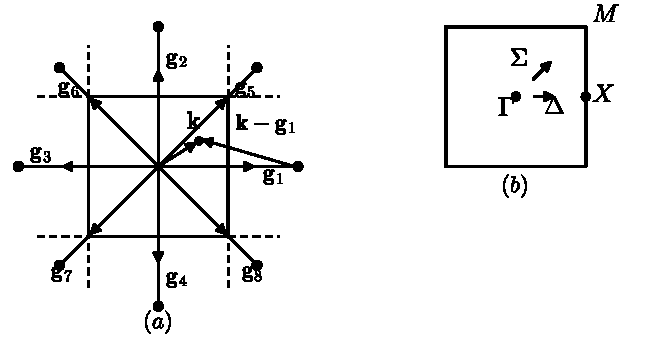
\includegraphics[width=0.72\textwidth]{fig_65.pdf}
\caption*{图 65\quad ($a$) 倒格子空间中的一般点 $\mathbf{k}$；($b$) 正方区中的对称点和对称线。}
\end{figure}
情形下，是乘上像 $1/\sqrt{3}$ 这样一个数后的相同系数。它还告诉我们，在哪些点上可以预期能级之间出现简并。例如，在点 $M$ 处，设有四个 O.P.W. 或 A.P.W. 在能量上简并（对应于图 65 中的 $\mathbf{k}$、$(\mathbf{k}-\mathbf{g}_5)$、$(\mathbf{k}-\mathbf{g}_1)$ 和 $(\mathbf{k}-\mathbf{g}_2)$）。它们会被与晶格势相联系的微扰所劈裂——但可以证明，一个二重简并总会保留下来。当我们画等能面时，这一信息极有帮助。

有一类问题中群论至关重要。在重原子中我们知道存在很强的\emph{自旋–轨道相互作用}（spin–orbit interaction）——一个形如 $\lambda\mathbf{L}\cdot\mathbf{S}$ 的算符，其中 $\mathbf{S}$ 是电子的自旋算符，$\mathbf{L}$ 是轨道角动量算符。在自由原子中，它的作用是消除某些具有同一空间波函数、但电子自旋相反的状态之间的简并。例如，原子的 $P$ 态分裂成 $P_{\frac{3}{2}}$ 和 $P_{\frac{1}{2}}$ 两个态，分别对应于总角动量 $j=\frac{3}{2}$ 和 $j=\frac{1}{2}$。

在构造能带时我们所作的假定是：自旋无关紧要；我们只用一个空间波函数，并且对每个 $\psi_{\mathbf{k}}$ 假定可以把两个自旋相反的电子放进具有这个波函数的两个态里。自旋–轨道相互作用可能解除这些态之间的简并。然而要注意，\emph{时间反演对称性}（time reversal symmetry）这条基本量子原理，总会在任何 Bloch 态 $\psi_{\mathbf{k}}(\mathbf{r})$ 与其复共轭 $\psi_{\mathbf{k}}^*(\mathbf{r})$ 之间保留 \emph{Kramers 简并}（Kramers degeneracy）——后者描写的是电子的波矢和自旋两者都反转了的态。对“无自旋”粒子，这意味着 $\mathcal{E}(\mathbf{k})=\mathcal{E}(-\mathbf{k})$，与晶格的点群对称性无关。

在区中的一般点上，$\psi_{\mathbf{k}}$ 本身不简并；此时若晶格势具有反演中心，自旋–轨道相互作用并不把自旋相反的态分开。这是因为，在态 $\psi_{\mathbf{k}}(\mathbf{r})$ 中反转自旋，等价于考察 $\psi_{\mathbf{k}}(-\mathbf{r})$，而后者具有相同的能量。

但是区中有一些特殊点，自旋–轨道效应在这些点上可能相当重要。最有趣的情形是区的中心，一个具有立方对称性的点。在紧束缚模型中，我们可以用 $p$ 轨道来构造一条‘p 带’。但原子有三个简并的 $p$ 态，所以我们有三条这样的带——比如说，对应于原子的 $p_x$、$p_y$ 和 $p_z$ 轨道。这三条带在 $\mathbf{k}=0$ 处简并；在该点上它们恰好被立方对称性互相变换。每条带的每个态又是二重自旋简并的，所以总共有六重简并。

当我们引入自旋–轨道相互作用时，发现这个六重简并被劈裂成一个四重能级和一个二重能级。实际上，现在我们应当用原子态 $p_{\frac{3}{2}}$——它是四重简并的——和 $p_{\frac{1}{2}}$——它是二重简并的——来构造我们的能带。有趣的是看看当我们沿某个任意方向离开 $\mathbf{k}=0$ 时会发生什么。如果
存在反演对称性，那么每条能级仍然是二重简并的，如图 66($b$) 所示。我们可以说，$j=\frac{3}{2}$ 的带再次分裂成 $m_j=\pm\frac{3}{2}$ 的带（比如说，沿传播方向计量）和 $m_j=\pm\frac{1}{2}$ 的带。如果没有反演对称性，它们还会像图 66($c$) 那样进一步分裂；通过自旋–轨道相互作用，电子自旋变得对晶体势沿传播方向所含的“螺旋”成分敏感了。

\begin{figure}[H]
\centering
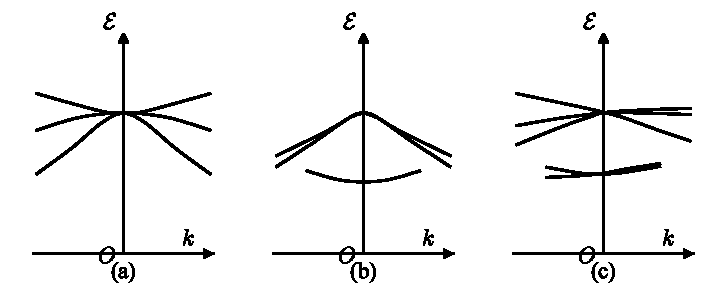
\includegraphics[width=0.72\textwidth]{fig_66.pdf}
\caption*{图 66\quad 自旋–轨道相互作用对区中心附近 $p$ 型能级的影响：($a$) 6 个能级在 $\mathbf{k}=0$ 处简并；($b$) 在具有反演对称性的晶格中，自旋–轨道相互作用使所有态保持二重简并；($c$) 没有反演对称性时，简并被完全解除。}
\end{figure}

这些效应在诸如 Ge 或 InSb 这类半导体的价带顶部十分重要。在前一种情形，图 66($b$) 成立；在后一种情形，不存在反演中心，区中心处的简并当我们沿任意方向离开时就解除。劈裂的实际符号和大小，可以从自由原子能级中相应效应的符号和大小推测出来。

要作定量计算，方便的办法是把自旋–轨道相互作用 $\lambda\mathbf{L}\cdot\mathbf{S}$ 当作微扰来处理。在区中心附近，它主要作用在 Bloch 函数的周期部分 $u_{\mathbf{k}}$ 上，后者满足方程 (3.38)。事实上，我们可以利用这个方程与普通 Schrödinger 方程的相似性，把附加项
\begin{equation*}
-\frac{i\hbar^2}{m}\,\mathbf{k}\cdot\nabla=\frac{\hbar}{m}\,\mathbf{k}\cdot\mathbf{p}\tag{3.83}
\end{equation*}
当作状态 $u_{\mathbf{0}}$ 上的一个附加微扰（对小的 $\mathbf{k}$ 值），从而不必完整算出整个能带结构，就能细致地计算自旋–轨道劈裂。这就是所谓的 \emph{$\mathbf{k}\cdot\mathbf{p}$ 方法}（$\mathbf{k}\cdot\mathbf{p}$ method）。

 % 本文件由 scripts/assemble.py 自动装配，勿手改（改 parts/ 后重跑）
% 第4章 固体的静态性质

% 第4章 STATIC PROPERTIES OF SOLIDS

\chapter{固体的静态性质}

\epigraphbook{停住吧，你们这永远运转的天球……}{MARLOWE}

\section{固体的类型：能带图像}

我们已经花了相当长的篇幅讨论电子结构理论，因为它决定了固体的类型及其宏观性质。

考虑一条完全填满的能带，其上方存在一个能隙。这就是基态；由对称性可知，它必然处于这样的状态：没有电流在流动。要产生电流，可以施加一个电场，它把一些电子激发到代表净电流的态上。但如果存在能隙，就需要有限的激发能才能把电子抬升、越过能隙进入上面一条能带。这份能量无法由小的恒定电场提供，所以这种固体将是\emph{绝缘体}（insulator）。

\begin{figure}[H]
\centering
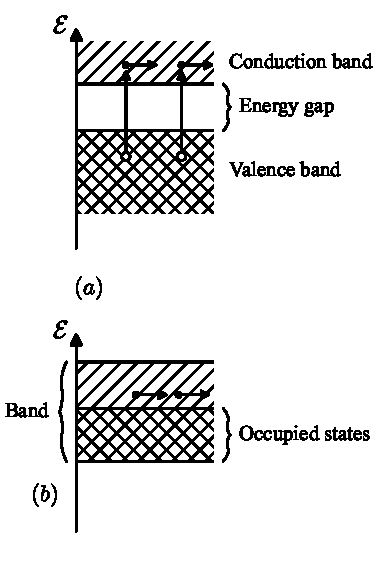
\includegraphics[width=0.72\textwidth]{fig_67.pdf}
\caption*{图 67\quad (a) 半导体中载流子的激发。(b) 金属中传输电流的电子。}
\end{figure}

但假定能隙 $\mathcal{E}_{\mathrm{gap}}$ 很小。在温度 $T$ 下，将会有一个小而非零的电子密度，它们被热涨落激发到上面的能带中去——这一密度由形如 $\exp(-\mathcal{E}_{\mathrm{gap}}/kT)$ 的 Boltzmann 因子刻画。这些电子很容易传输电流，于是材料将具有可观察的电导率，并且随温度升高迅速增大。这时我们就说，我们得到的是\emph{半导体}（semiconductor）。

如果一条能带并未填满，例如在一价金属中，那么尽管系统的真实基态在 $\psi_{\mathbf{k}}$ 与 $\psi_{-\mathbf{k}}$ 之间是对称的、因而同样不载流，但在占据能级顶端之上能量距离为无穷小处，就存在着载流的态。此时电导率很高，而且对温度的依赖不大——温度只是在它支配电子散射机制这一点上才起作用。这样我们便得到了典型的\emph{金属}。

要判断一个具有给定结构的固体究竟是金属、半导体，还是实质上的绝缘体，我们回顾一下（§1.6）：一个布里渊区所包含的“允许的 k 矢量”——即彼此不同的电子波函数——恰与晶体中晶胞的数目一样多。而每个被允许的空间波函数可以容纳 2 个自旋相反的电子。于是，若单位体积中有 $N$ 个晶胞，则每条能带有 $2N$ 个电子态，即每条能带在每个晶胞摊到 2 个电子态。数一数每个晶胞中的电子数，我们就能对固体可能具有的性质作出若干估计。

(i) 每个晶胞有\emph{一个}自由电子的固体总是金属。典型的是一价金属——碱金属 Li、Na、K、Rb、Cs，以及贵金属（noble metals）Cu、Ag、Au。它们都恰好只有一条半满的能带，或者说半满的区。

(ii) 每个晶胞有\emph{奇数}个电子的固体总是金属。于是，在 Al、Ga、In、Tl 中每个原子有 3 个电子，只够填满一条半的能带。

但注意，As、Sb、Bi 每个原子有 5 个电子，它们结晶成的结构每个晶胞含 2 个原子，所以这条规则用不上。事实上，它们是半金属（semi-metal）：10 个电子几乎恰好填满 5 条能带，但第 5 条能带并未完全填满，还有少许\emph{交叠}进入第 6 条能带，因此不论温度如何，总有少量电子可以传导电流。

(iii) 每个晶胞有\emph{偶数}个电子的固体则不一定是绝缘体。这是因为各条能带在能量上可以交叠。让较低的能带留着不填满、而让一部分电子进入上面的能带，在能量上可能是有利的。

\begin{figure}[H]
\centering
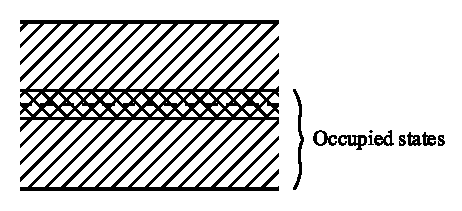
\includegraphics[width=0.72\textwidth]{fig_68.pdf}
\caption*{图 68\quad 相互交叠的能带。}
\end{figure}

\begin{figure}[H]
\centering
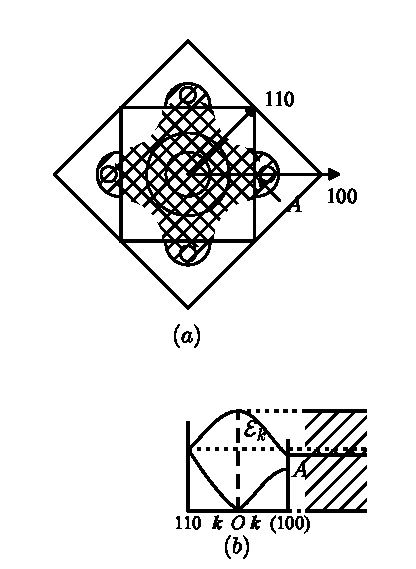
\includegraphics[width=0.72\textwidth]{fig_69.pdf}
\caption*{图 69\quad 二价金属的交叠能带：(a) 扩展区图式；(b) 简约区中能量随 k 的变化。}
\end{figure}

在一维情形这不会发生：各条能带彼此完全分开（见图 38）。但在真实金属中，我们可能遇到图 69 所描绘的情况。虽然在任何特定地点越过区边界时都可能有能隙，但第 2 条能带的最低部分（例如在 $A$ 处）可能位于第 1 条能带最高部分之下，于是电子在 $A$ 处“溢出”区的边界，而区的角隅则空着。

这一点在扩展区图式的近自由电子（N.F.E.）模型中很容易看清（参见 §3.3）。一个容纳 $2N$ 个态的球面会在若干处与区边界相交。如果势（或赝势）相应的 Fourier 分量很小，其效果只不过是：当球面的各部分穿过每条区边界时把它们截断
\begin{figure}[H]
\centering
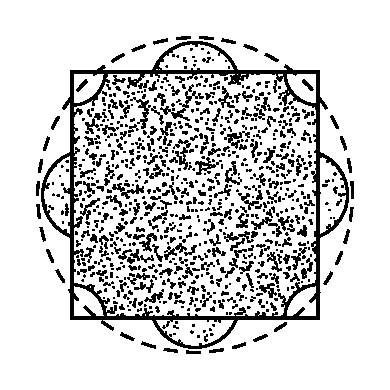
\includegraphics[width=0.72\textwidth]{fig_70.pdf}
\caption*{图 70\quad 被区边界截断的自由电子球。}
\end{figure}
——而费米面的其余部分实际上保持不变。对于通常的电学性质而言，费米面的这些碎片可以在简约区和重复区中重新连接起来，这一事实无关紧要。

(iv) 结果发现，所有\emph{二价}元素都是金属：能隙还不够大，不足以把电子都容纳在单一区内。但其中一些（Sr、Ba）是劣导体，其交叠可能很小。

(v) \emph{四价}元素或者是金属，或者是半导体。有趣的情形是 Sn，它在一种相中是金属，在另一种相中是半导体。晶体结构的改变会改变区的形状，从而改变出现足够大的能隙以容纳全部电子的可能性。在周期表第 IV 族中有一段有趣的递变：从 C——作为金刚石，它形成的半导体能隙如此之大，以致在实践中成了绝缘体——到 Si 和 Ge 这两种半导体，到既为金属又为半导体的 Sn，再到金属 Pb。所有这些元素的能带结构都可以用 N.F.E. 模型表示；半导体就是能隙很大且没有交叠的“金属”。

\begin{figure}[H]
\centering
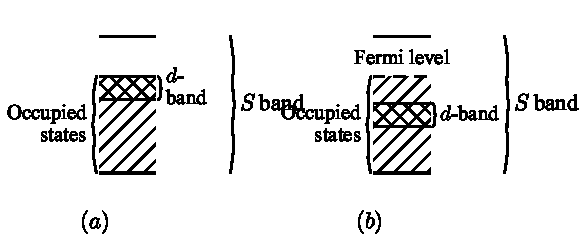
\includegraphics[width=0.72\textwidth]{fig_71.pdf}
\caption*{图 71\quad (a) 过渡金属。(b) 贵金属。}
\end{figure}

(vi) \emph{过渡元素}（transition elements），例如铁族的 Cr、Mn、Fe、Co、Ni，以及周期表中位置更高的其他各族，其特征在于内层 $d$ 壳层未满。例如在原子 Fe 中，尽管外层 $4s$ 态里还有另外 2 个电子，$3d$ 壳层的 10 个态中只有 6 个被填充。当原子聚到一起构成固体或液体时，这些外层价电子进入一条宽的“$s$ 能带”，与普通金属中的 N.F.E. 导带没有太大差别。在某些方面（见 §10.5），$d$ 电子的表现仍好像定域在各自的原子实中：对稀土族（rare earth group）的 $4f$ 电子来说，这实际上是一个极好的近似。但 $d$ 轨道实际上必须在原子之间相互交叠，以形成一条窄的“$d$ 能带”，每个原子至多可容纳 10 个电子。正如我们在 §3.10 中看到的，这条能带与 $s$ 能带交叉并杂化；严格说来，这种复杂的能带结构是与原先原子 $d$ 能级处的共振相联系的，不能分解成分开的 $s$ 能带与 $d$ 能带。

尽管如此，比如说，下述说法仍然是自然的：两条能带都不满，故材料呈金属性，导电主要依靠“$s$ 电子”（图 71(a)）。在贵金属中，$d$ 态实际上是满的，但它们在价电子的普通 N.F.E. 能带之内、费米能级以下几电子伏处生成一条共振 $d$ 能带（图 31(b)）。这对那些本会是简单一价金属的材料有显著影响（见 §9.4）。

\section{固体的类型：键图像}

用能带模型，我们所能轻松走到的程度也就到此为止了。但让我们再来看一看半导体 Si 和 Ge。它们具有“金刚石结构”（diamond structure），与 F.C.C.（面心立方）相像（见 §1.3），只不过
\begin{figure}[H]
\centering
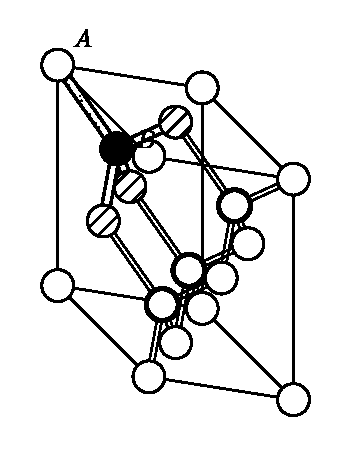
\includegraphics[width=0.72\textwidth]{fig_72.pdf}
\caption*{图 72\quad 金刚石结构中的四面体键。}
\end{figure}
每个晶胞有两个原子。取一个以 $A$ 为角隅的 F.C.C. 格子，在沿立方体主对角线 $1/4$ 处的 $B$ 点放上另一个原子。让这个新原子作为第二个 F.C.C. 格子的角隅，与第一个相互贯穿。

这种结构与 F.C.C. 格子有相同的布里渊区。现在每个晶胞有 8 个电子，所以需要填满 4 条能带。如果从紧束缚模型的观点来看这 4 条能带，就会发现它们来自自由原子的 4 个轨道——Si 中的 $3s$ 轨道和三个 $3p$ 轨道；Ge 中的 $4s$ 与 $4p$ 轨道。当原子聚到一起时，这些轨道交叉并组合，形成 4 条能量范围大致相同的能带（我们在 §3.11 中注意到，若不是自旋–轨道相互作用，其中三条在区中心应当是简并的）。再上面一条能带与这些\emph{价带}（valence bands）之间隔着约 1 eV 量级的能隙。

但这种 $s$ 轨道与 $p$ 轨道的组合在化学键理论中是众所周知的。人们知道，这些波函数可以组合起来，给出四个轨道波函数，每一个都指向一个四面体的顶点。人们还知道，诸如 CH$_4$ 之类分子的四面体对称性与\emph{共价键}（covalent bond）的形成相联系，即通过在这些 $s$-$p$ 杂化轨道中共享电子对而成键。再看图 72，我们看到 $B$ 处的原子恰好有 4 个最近邻，排在四面体的顶点上。它们每一个又同样与其近邻相连，如此等等：换言之，\emph{整个晶体就像一个巨大的共价键合的分子}。

能带结构计算证实了这一点。用少数几个 O.P.W.（正交化平面波）配上合适的赝势系数，就能与实验能带结构符合得相当好。所得的波函数倾向于把电子密度集中到“键”上。我们示意地把电子结构表示成图 73 的样子。每个 Ge 或 Si 离子与近邻共享 8 个电子。这些电子其实并不定域在键上。像金属中的自由电子一样，它们的波函数扩展到整个晶体。但在相邻离子之间的区域中，总有一团高度集中的电子云，等效于一对自旋相反的电子。

\begin{figure}[H]
\centering
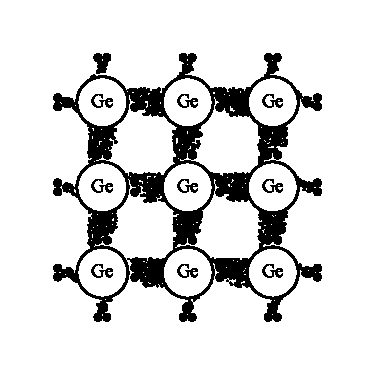
\includegraphics[width=0.72\textwidth]{fig_73.pdf}
\caption*{图 73\quad Ge 的电子结构（示意图）。}
\end{figure}

然而要注意，这在某种程度上是一个自我实现的预言。在配位数低的格子中，muffin-tin 近似（§3.7）并不适用，电子的势能在间隙区域内并非处处均匀。在任何自洽计算的尝试（参见 §5.2）中，电子电荷都会自动沿相邻原子球之间的连线聚集，那里正是间隙势最低之处。如果我们一开始就要解释这类晶体结构何以出现，那么一般的化学论证看来是必不可少的。

现在有趣的是把这幅图像稍加改动：把 Ge 换成 InSb。我们记得 In 和 Sb 与 Ge 处在周期表的同一横行，所以它们具有相同的闭壳层基础芯。但 In 只有 3 个外层电子，Sb 有 5 个。它同样形成一种类金刚石
\begin{figure}[H]
\centering
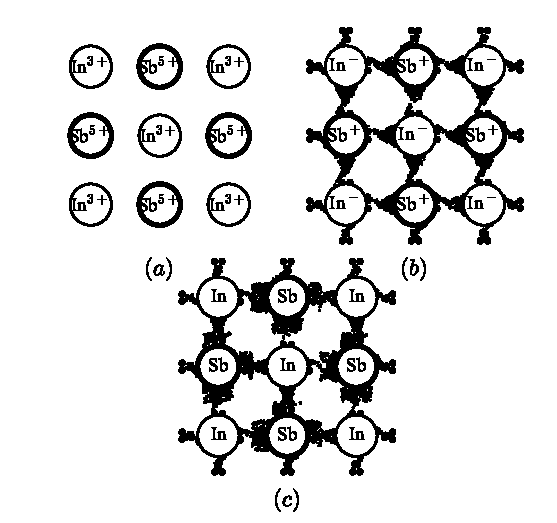
\includegraphics[width=0.72\textwidth]{fig_74.pdf}
\caption*{图 74\quad 锑化铟（示意图）。(a) 裸离子。(b) 带有对称的键。(c) 被离子上残余电荷极化的键电子。}
\end{figure}
的晶格，只不过现在 In 占据全部 $A$ 位，而 Sb 占据全部 $B$ 位。示意地，我们得到如图 74(a) 那样的离子排列。

在许多方面它与 Ge 结构如此相像，以至于我们可以把每原子 8 个电子放入同样的“键-带”轨道，如图 74(b)。但这会留下一些残余电荷：Sb 上的电荷没有被它周围平均 4 个电子完全中和，而 In 上则多出一点额外的负电荷。不过，这些效应很容易通过让电荷云向 Sb 略微收缩、并离开 In 来容纳，如图 74(c)。这种化合物是半导体，基本能带结构与 Ge 相仿，尽管结果表明其能隙较小。它是典型的 \emph{III–V 族金属间化合物}（intermetallic compound）。

现在转到 ZnS，它是一种 \emph{II–VI 族化合物}——Zn 有 2 个电子，S 有 6 个。它形成的晶体与 InSb 完全相似——事实上，这就叫作\emph{闪锌矿}（zinc-blende）结构——而且也是半导体。但现在，电子对 $\mathrm{S}^{6+}$ 离子的静电吸引又因\emph{电子亲和势}（electron affinity）而增强：这个离子所能看到的 8 个电子倾向于收得更紧，力图构成一个完整的闭壳层，而让 $\mathrm{Zn}^{2+}$ 离子几乎不含电子。

\begin{figure}[H]
\centering
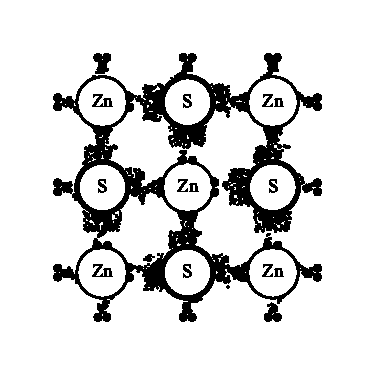
\includegraphics[width=0.72\textwidth]{fig_75.pdf}
\caption*{图 75\quad 硫化锌（示意图）。}
\end{figure}

这一过程在比如 CuCl 中走到了彻底的地步。Cu 原子完全失去它的电子，这个电子拿去构成 $\mathrm{Cl}^{-}$ 闭壳层。于是我们得到实际上相互独立的离子 $\mathrm{Cu}^{+}$ 和 $\mathrm{Cl}^{-}$，没有任何自由电子剩下。它将结晶成如图 76 那样的正负交替的晶格。但此时的内聚已不再与键相联系。它本质上来自离子间的静电吸引，可以按 §2.3 的方法计算。最近邻的四面体排列现在无关紧要了——要点是围绕一个负离子尽可能多地挤入正离子，反之亦然。\emph{离子型固体}倾向于结晶成 NaCl 和 CsCl 那样的结构。

对于这种晶体中的价电子，谈论“能带结构”究竟还有多大意义，是一个微妙的问题。这些电子的波函数紧紧定域在各自的离子上，不表现出诸如自由载流子“空穴”迁移率（参见 §6.6）那样的“Bloch 函数”性质；“能隙”大致就相当于金属原子的第二电离势。当然，被激发到这个隙之上的电子，其行为会更像普通导带中可迁移的载流子。

实际上，离子型固体与共价型固体之间并没有截然的分界。在 III–V 或 II–VI 族化合物中总存在某种程度的离子性。即便是离子晶体，也能表现出与半导体相似的性质。

\begin{figure}[H]
\centering
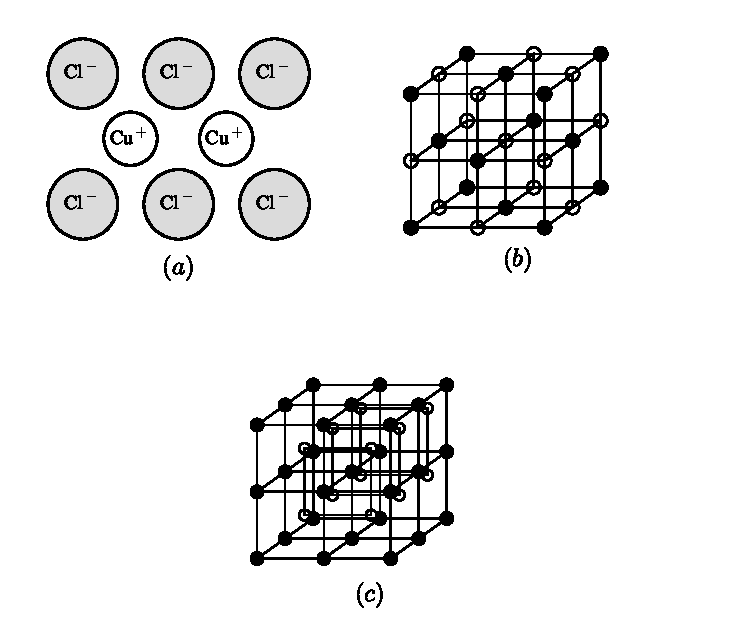
\includegraphics[width=0.72\textwidth]{fig_76.pdf}
\caption*{图 76\quad (a) 氯化铜（示意图）。(b) NaCl 结构。(c) CsCl 结构。}
\end{figure}

这并没有穷尽固体的分类。还有\emph{分子型晶体}（molecular crystals），其构造单元是稳定的中性分子，例如 CH$_4$，靠彼此间的 van der Waals 引力凝聚在一起。还有一类特殊的\emph{氢键型结构}（hydrogen-bonded structures），其中分子基团之间的力通过一个共享的质子来传递。这些固体通常由分子的化学性质所支配。除了可作为简单晶体范式的稀有气体固体之外，它们往往结构复杂，其性质超出了本书的范围。

\section{内聚性}

固体理论的一个主要目标，是说明固体何以是其所是——也就是说，要证明把一大堆，比如说，Na 原子放进一个盒子里，它们会凝聚成一块金属钠晶体。这个目标过于雄心勃勃；但我们还是可以研究固体能量学的某些侧面。特别是，我们可以尝试计算固体的内聚能（cohesive energy）——从分离原子集合体的能级量起的能量——并将它与实验相比较，或者与由同样原子构成的其他假想固体（点阵常数不同，或晶体晶格不同）的能量相比较。

例如，注意到分子晶体的内聚能很小——量级为每分子 0·1 eV——我们就证实了 van der Waals 力之弱。氢键型晶体（典型如 H$_2$O）的内聚要高一些——比如每分子 0·5 eV。这两类固体的熔点都很低。金属则更够得上典型的“固体”，内聚能介于每原子 1 至 5 eV 之间；而离子型和共价型固体结合得非常牢固，能量达每原子 10 eV 的量级。

着手计算内聚能所依循的原理，从前几章已可看出。例如对离子晶体，我们先为该结构算出 Madelung 常数（式 (2.27)），从而把静电力的贡献确定为
\begin{equation*}
\mathcal{E}=-\frac{1}{2}N\alpha\frac{e^{2}}{a}.
\tag{4.1}
\end{equation*}
这个能量显然趋于使固体塌缩，即使点阵常数 $a$ 减小。但这个力受到离子实之间排斥的对抗——这种排斥常用如下形式的势来代表：
\begin{equation*}
\phi(R)=B\exp(-R/\rho)
\tag{4.2}
\end{equation*}
其中 $R$ 为离子间的距离。

把这两项拼在一起、把固体的总能量估计为 $a$ 的函数，是一个不足道的计算。它可以同总内聚能以及固体压缩系数的实验值相比较。遗憾的是，对给定的一对离子，参数 $B$ 与 $\rho$ 不可能从第一性原理以任何高精度算出；我们至多只能导出一组经验值，它们或多或少地与对各种不同晶体——其中离子按一切可能的组合配成对——的观测相一致。这个唯象方案于是可以解释为给出若干元素的离子半径（ionic radii）。

共价固体的内聚能是一个复杂得多的问题。原则上，可以通过计算能带结构、再求出每个电子态能量的贡献而把它找出来。实际上，更容易的做法是证实：晶体的总能量相当接近各共价键能量之和，而晶格谱可以由在声子模中弯曲和/或拉伸这些键所需的力导出。就金刚石而言，这种符合是极好的。如果我们懂得了共价键的能量学，那么在理解半导体内聚能的道路上，我们就已经走了很远了。

既然共价固体的内聚几乎完全依赖于键的化学饱和性，结构就不一定非要具有晶体序不可。在一种没有长程序的网络中，常常也能让每个原子以非常接近正确的几何组态获得正确数目的近邻。例如，普通的硅石玻璃（silica glass）就是这样的集合体：每个 Si 原子都位于一个由氧构成的四面体的中心，而每个氧原子几乎正好位于两个 Si 原子的连线上（图 77）。这个网络在化学上和动力学上都显然是稳定的，但应当如何从能带的观点描述它的内聚，却不清楚。

\begin{figure}[H]
\centering
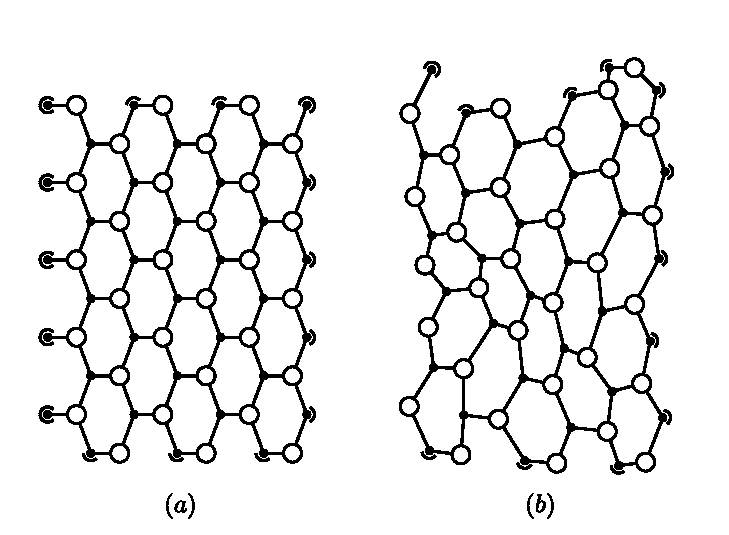
\includegraphics[width=0.72\textwidth]{fig_77.pdf}
\caption*{图 77\quad 共价键网络：(a) 晶态；(b) 玻璃态。这是 SiO$_2$ 的二维类似物。}
\end{figure}

金属内聚（metallic cohesion）则是一个微妙得多的现象。大体上我们可以说，把每个电子从它在特定原子上的定域中解放出来，就增大了其位置坐标的不确定度；于是按 Heisenberg 原理，动量的散布便减小。这降低了电子的平均动能，从而把系统结合在一起。但是，总内聚能的计算属于整个金属理论中最难做对、也最难在原则上验证的问题之列。为了计入电子气体中的关联与交换这类复杂的多体效应（见 §5.8），切分这块“蛋糕”的办法有很多种。

在最简单的分析中，我们考虑两个方向相反的主要贡献。当原子彼此接近、相互交叠时，每个电子能够在更大的区域内运动，在其中它的平均势能较低。另一方面，当我们压缩电子气体时，费米能被推高，从而增大了电子的平均动能。在金属密度下，这两种力处于平衡。

\begin{figure}[H]
\centering
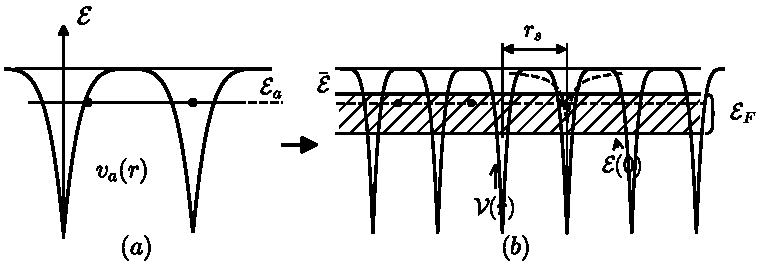
\includegraphics[width=0.72\textwidth]{fig_78.pdf}
\caption*{图 78\quad 内聚的 Wigner–Seitz 模型：(a) 单原子气体；(b) 金属。}
\end{figure}

为了说明这个论证，设想我们从诸如 Na 这样的碱金属的自由原子出发。每个原子有一个价电子处在原子势 $v_{a}(r)$ 的最低束缚态 $\mathcal{E}_{a}$ 上；在离子实之外，这个势的行为应当如同库仑势 $-e^{2}/r$。固体金属中的传导电子所感受到的晶体势 $\mathcal{V}(\mathbf{r})$ 显然会比这类函数的单纯叠加复杂得多，因为它现在还必须把“其他”传导电子等等的贡献包括进来。然而，作为一种粗糙近似，让我们假定：所选的这个电子凭其静电排斥，暂时把所有其他价电子都从它恰好所处的那个 Wigner–Seitz 原胞（§3.5）的整个范围中排除出去；而晶体中所有其余原胞这时都含有电子，恰好把它们静电中和。换句话说，原子交叠的效应和电子关联等等的效应，都通过取 $\mathcal{V}(\mathbf{r})$ 在每个原胞中等于 $v_{a}(r)$（对 $r\leqslant r_{s}$）来模拟（图 78）。

在原子球的实际边界处，这显然是一个糟糕的近似。尽管如此，其净效果是晶体中电子的平均势能大幅降低。更精确地说，运用 Wigner–Seitz 元胞近似可以证明：导带底 $\mathcal{E}(0)$ 必定位于比这个势垒的能量稍低之处——即位于 $-e^{2}/r_{s}$ 以下的某个能级上。于是当 $r_{s}$ 减小时我们正在赢得势能。

排斥项的理论对自由电子气体来说是不足道的。由 §3.1 的公式我们容易证明：能量态密度（density of states in energy）——单位能量间隔内的电子态数目——由下式给出：
\begin{equation*}
\mathcal{N}(\mathcal{E}_{F})=\frac{3}{2}\frac{n}{\mathcal{E}_{F}}
\tag{4.3}
\end{equation*}
其中 $n$ 是费米能为 $\mathcal{E}_{F}$ 的电子的密度。由此可得
\begin{equation*}
\mathcal{N}(\mathcal{E})\propto\mathcal{E}^{1/2},
\tag{4.4}
\end{equation*}
从而每个电子的平均能量为
\begin{equation*}
\bar{\mathcal{E}}_{\text{kin.}}=\frac{3}{5}\mathcal{E}_{F},
\tag{4.5}
\end{equation*}
它按 $1/r_{s}^{2}$ 变化。

把这两项合并起来，如图 79 那样，我们看到在某个 $r_{s}$ 值处出现一个极小；这个值应当就是实际金属中的原子半径，并且应当给出总内聚能的合理估计。由这个粗糙论证得到的结果至少数量级是对的，说明这个一般性解释在原则上站得住脚。

\begin{figure}[H]
\centering
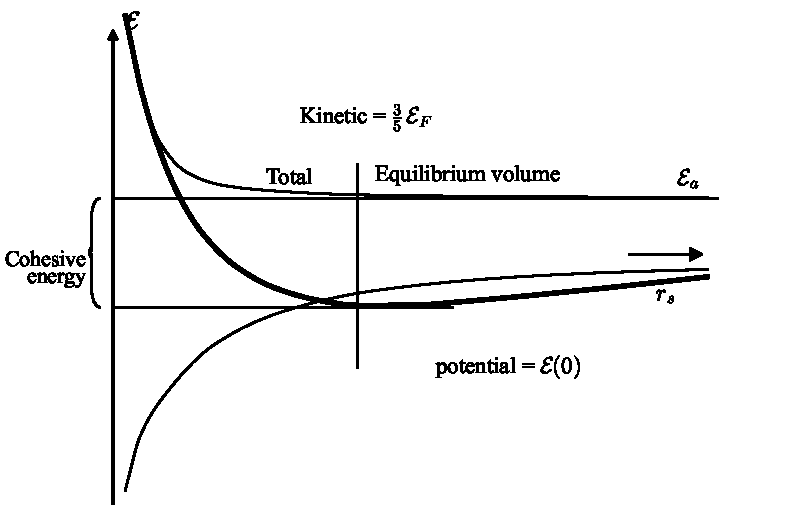
\includegraphics[width=0.72\textwidth]{fig_79.pdf}
\caption*{图 79\quad 金属内聚的诸贡献，表为原子间距的函数。}
\end{figure}

然而有意思的是，所有碱金属的内聚能都非常接近 $\frac{2}{5}\mathcal{E}_{F}$。由这个经验事实，我们从式 (4.5) 推断：金属中的费米能级与能带所由导出的那个原子能级的能量近似重合。这正是 L.C.A.O. 理论中半满能带所应有的结果，如式 (3.30)。对金属内聚的另一种解释则是：电子得以成对地进入 Bloch 态，两电子自旋相反，而不必像它们各自束缚于分立的原子轨道时那样付出静电能量的代价。

内聚力的性质影响固体的弹性和塑性。共价固体刚硬而脆，因为键的方向性阻碍剪切运动，使一个原子无法从另一个原子旁边滑过——正如位错穿过晶格的迁移那样。离子晶体则更具塑性，只要它们是完善的纯晶体（不过普通晶体可能由于生长中带入的缺陷而是脆性的）。静电力没有方向性，因此除了受离子大小的阻碍之外，它们允许离子四处移动。金属是最具塑性的固体，允许位错自由运动，因为电子气体的费米能倾向于使离子彼此保持距离，而内聚能主要是堆积密度的函数。对严格晶格规则性的局域偏离很容易被容纳下来。

\section{刚性能带模型与态密度}

为什么许多金属会以不同的相出现，具有不同的晶体结构，并且随温度变化而从一个相转变到另一个相？与晶体热激发相联系的能量很小——量级为每原子 0·1 eV。不同结构的能量差必定很小。的确，我们上面基于 Wigner–Seitz 公式和紧束缚（tight-binding）公式的粗糙论证，无法区分密度相同而晶体结构不同的相。有意思的是，金属熔化时密度变化不大；上述论证对结构如此不敏感，以至于它们对液态金属同样适用——液态金属可以十分简单地描述为一种无规堆积的球形离子集合体，靠自由电子构成的“胶”黏结在一起。

不过，有一个现象体现了一条关于固体结构能量的原理。考虑下表：

%TAB{}: 代表性合金相的晶体结构与电子/原子比（原书此表未编号）
\begin{table}[H]
\centering
\caption*{合金的晶体结构、代表性合金与电子/原子比}
\begin{tabular}{lccc}
\toprule
结构 & 体心立方 & “$\gamma$ 黄铜” & 六角密堆积 \\
\midrule
合金 & AgZn & Ag$_5$Zn$_8$ & AgZn$_3$ \\
 & Cu$_3$Al & Cu$_9$Al$_4$ & — \\
 & Cu$_5$Sn & Cu$_{31}$Sn$_8$ & Cu$_3$Sn \\
\midrule
电子/原子 & $\frac{3}{2}=1\cdot5$ & $\frac{21}{13}=1\cdot615$ & $\frac{7}{4}=1\cdot75$ \\
\bottomrule
\end{tabular}
\end{table}

每一列指的是一个合金系列，各系列中的合金都具有相同的基本晶体结构，并且各自形成一个成分或多或少确定的稳定相。它们有什么共同之处？在底行我们给出电子数对原子数之比，它对每一列都是常数。例如在 Cu$_9$Al$_4$ 中，Cu 原子提供 9 个电子，4 个 Al 原子每个提供 3 个电子，合计 13 个原子 21 个电子。

这个现象所例示的，就是人们常在合金的刚性能带（rigid band）理论基础上讨论的 Hume–Rothery 定则（Hume–Rothery rules）。其论证是：把组元元素的价电子统统倒入单一的近自由电子（N.F.E.）能带中，这个能带类似于普通纯金属的能带（§3.3）。例如对 Cu$_{31}$Sn$_{8}$，这个假想金属每原子将拥有 1·615 个电子。

我们现在假定合金的布里渊区结构依赖于基本晶格，而不太依赖于占据格点的实际离子。结果表明，对“$\gamma$ 黄铜”结构，这个区的形状和大小恰好使它同一个容纳每原子 1·615 个传导电子的自由电子球相切。于是可以预期，在这些固体中费米面会在相当大的面积上接触区边界，但多半还没有破入下一个区。由于正好在区边界之内的态比具有同一波矢的自由电子能量更低，金属若取这种结构便可在内聚能上获益。关于许多纯金属和复杂合金相之晶体结构的这个解释非常利落，常被算作金属电子理论的一项胜利。遗憾的是，把近自由电子（N.F.E.）模型用于诸如 Cu、Ag、Au 这样的金属是有异议的，因为在纯金属中费米面本来就接触区边界（见 §9.4）。刚性能带模型本身的理论地位也存在一些疑问（见 §5.3），尽管在个别情形中有“区边界效应”的有力证据。

实际上，我们是说：结构使得费米能级落在一大段能量范围的顶端附近，在那里能量态密度很高。这个函数对自由电子气体已由式 (4.3) 给出。要计算实际金属的 $\mathcal{N}(\mathcal{E})$，我们必须求出布里渊区中逐级能量面之间所包围的体积。这个问题在形式上与 §2.5 中晶格谱的计算完全相同。

\begin{figure}[H]
\centering
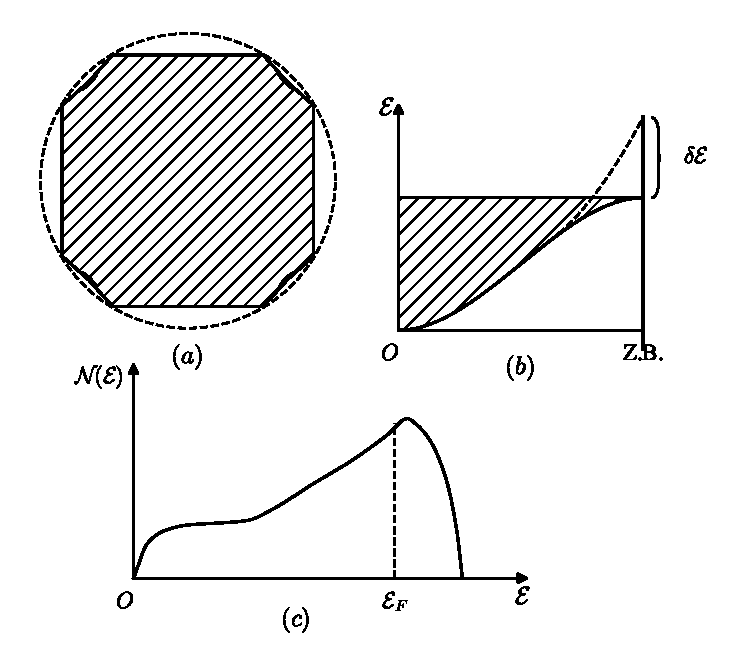
\includegraphics[width=0.72\textwidth]{fig_80.pdf}
\caption*{图 80\quad (a) 费米面接触区边界。(b) 能量降到自由电子值之下。(c) 费米能级靠近态密度的极大。}
\end{figure}

仿照式 (2.66)–(2.69) 的论证，我们可以写出
\begin{equation*}
\mathcal{N}(\mathcal{E})=\frac{1}{4\pi^{3}N\hbar}\int\frac{dS}{|\mathbf{v}_{\mathbf{k}}|},
\tag{4.6}
\end{equation*}
为此我们暂时定义一个具有速度量纲的矢量
\begin{equation*}
\mathbf{v}_{\mathbf{k}}=\frac{1}{\hbar}\nabla_{\mathbf{k}}\mathcal{E}(\mathbf{k}),
\tag{4.7}
\end{equation*}
即能量函数在 $k$ 空间中的梯度。出现在式 (4.6) 中的是这个矢量的模，须在能量为 $\mathcal{E}$ 的能量面上积分。

由于 $\mathcal{E}(\mathbf{k})$ 像 $\nu_{q}$ 一样是倒格子空间中的连续函数，具有倒格子的周期性，van Hove 定理（van Hove's theorem）的论证对它适用。的确，由于 $\mathcal{E}(\mathbf{k})$ 通常在区中心（即 $\nu_{q}$ 中声学支所在的区域）没有特殊的重根，$\mathcal{E}(\mathbf{k})$ 中的奇点必定包括所有四种类型的临界点——极大点、极小点以及两类鞍点。

一般地说，金属的态密度与自由电子值相去不远，只有过渡金属（transition metals）例外：狭窄的 $d$ 带（或几条 $d$ 带）必须能容纳每原子 10 个电子——所以其能量态密度必定远高于普通的 $s$ 带。既有证据表明这一点，也有证据表明 $d$ 电子对金属的内聚有贡献，正如我们从这个模型所预期的。

\section{电子的费米统计}

到目前为止，我们一直假定电子系统处于零温度；按照 Pauli 原理，我们把能级逐一填充，直到把全部电子用完为止，最后填到能量为 $\mathcal{E}_{F}$ 的费米能级。但我们从统计力学知道，电子服从费米–狄拉克统计（费米–狄拉克 statistics）；能量为 $\mathcal{E}$ 的能级被占据的概率是
\begin{equation*}
f^{0}(\mathcal{E})=\frac{1}{e^{(\mathcal{E}-\zeta)/kT}+1},
\tag{4.8}
\end{equation*}
其中 $\zeta$ 是费米势（Fermi potential），即化学势，或每个电子的自由能；只要电子气体处于热力学平衡，它在整个材料中就必须是常数。

设有 $\mathcal{N}(\mathcal{E})\,d\mathcal{E}$ 个态处在能量间隔 $d\mathcal{E}$ 内。若 $n$ 是电子的总密度（每单位晶体体积），则必须有
\begin{equation*}
n=\int_{0}^{\infty}f^{0}(\mathcal{E})\,\mathcal{N}(\mathcal{E})\,d\mathcal{E}.
\tag{4.9}
\end{equation*}
这两个方程定出 $\zeta$ 的值，从而定出整个分布。

在绝对零度下这是不足道的：容易看出，若 $\mathcal{E}<\zeta$，则 $f^{0}(\mathcal{E})$ 等于 1；而当 $\mathcal{E}>\zeta$ 时它为零。于是有
\begin{equation*}
n=\int_{0}^{\zeta}\mathcal{N}(\mathcal{E})\,d\mathcal{E}=\int_{0}^{\mathcal{E}_{F}}\mathcal{N}(\mathcal{E})\,d\mathcal{E},
\tag{4.10}
\end{equation*}
这就是费米能级定义的数学表述：
\begin{equation*}
\zeta=\mathcal{E}_{F}\quad\text{当}\quad T=0.
\tag{4.11}
\end{equation*}

要把 $\zeta$ 表为 $T$ 的函数，原则上需要知道 $\mathcal{N}(\mathcal{E})$。但在金属中分布是高度简并（degenerate）的，即 $kT\ll\mathcal{E}_{F}$。这时我们可以采用如下的数学技巧：——

设有如下形式的积分需要求值：
\begin{equation*}
I=\int_{0}^{\infty}g(\mathcal{E})\,f^{0}(\mathcal{E})\,d\mathcal{E},
\tag{4.12}
\end{equation*}
其中 $g(\mathcal{E})$ 是能量的某个函数。分部积分。我们得到
\begin{equation*}
I=\left[G(\mathcal{E})f^{0}(\mathcal{E})\right]_{0}^{\infty}-\int_{0}^{\infty}G(\mathcal{E})\frac{\partial f^{0}}{\partial\mathcal{E}}\,d\mathcal{E},
\tag{4.13}
\end{equation*}
其中
\begin{equation*}
G(\mathcal{E})\equiv\int_{0}^{\mathcal{E}}g(\mathcal{E})\,d\mathcal{E}.
\tag{4.14}
\end{equation*}
第一项在两个极限下都为零（只要把能量原点取得足够低，就可以令 $g(0)=0$）。

剩下的积分比较容易对付；由于 $\partial f^{0}/\partial\mathcal{E}$ 在 $\mathcal{E}=\zeta$ 处有一个对称的峰，它在那一带的行为宛如一个宽度为 $kT$ 的 $\delta$ 函数（delta-function）。于是，我们把 $G(\mathcal{E})$ 在这一点作 Taylor 展开：
\begin{equation*}
G(\mathcal{E})=G(\zeta)+(\mathcal{E}-\zeta)G'(\zeta)+\tfrac{1}{2}(\mathcal{E}-\zeta)^{2}G''(\zeta)+\dots,
\tag{4.15}
\end{equation*}
并代入式 (4.13)。我们得到
\begin{equation*}
I=G(\zeta)\int_{0}^{\infty}\left(-\frac{\partial f^{0}}{\partial\mathcal{E}}\right)d\mathcal{E}+G'(\zeta)\int_{0}^{\infty}(\mathcal{E}-\zeta)\left(-\frac{\partial f^{0}}{\partial\mathcal{E}}\right)d\mathcal{E}+\dots.
\tag{4.16}
\end{equation*}
但是
\begin{equation*}
\int_{0}^{\infty}\left(-\frac{\partial f^{0}}{\partial\mathcal{E}}\right)d\mathcal{E}=f^{0}(0)-f^{0}(\infty)=1,
\tag{4.17}
\end{equation*}
所以一级近似是
\begin{equation*}
I\approx G(\zeta)=\int_{0}^{\zeta}g(\mathcal{E})\,d\mathcal{E},
\tag{4.18}
\end{equation*}
这正是我们在 $T=0$ 时本应得到的结果。

\begin{figure}[H]
\centering
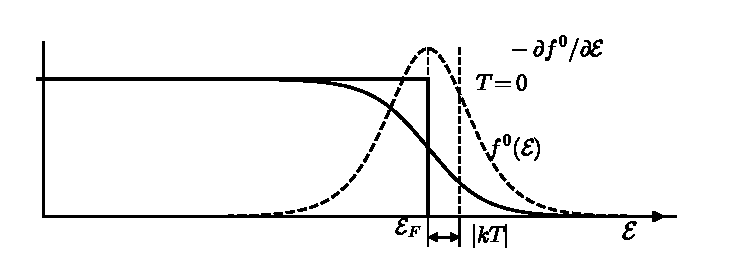
\includegraphics[width=0.72\textwidth]{fig_81.pdf}
\caption*{图 81\quad 费米–狄拉克函数及其导数：$T=0$ 时与有限温度下的情形。}
\end{figure}

式 (4.16) 中的普遍项含有积分
\begin{align*}
F_{n}&=\frac{1}{n!}\int_{0}^{\infty}(\mathcal{E}-\zeta)^{n}\left(-\frac{\partial f^{0}}{\partial\mathcal{E}}\right)d\mathcal{E}\\
&=\frac{(kT)^{n}}{n!}\int_{0}^{\infty}\left(\frac{\mathcal{E}-\zeta}{kT}\right)^{n}\frac{\exp\{(\mathcal{E}-\zeta)/kT\}}{\left[\exp\{(\mathcal{E}-\zeta)/kT\}+1\right]^{2}}\,d\!\left(\frac{\mathcal{E}-\zeta}{kT}\right)\\
&=\frac{(kT)^{n}}{n!}\int_{-\infty}^{\infty}\frac{z^{n}\,dz}{(e^{z}+1)(1+e^{-z})}\\
&=\left\{\begin{array}{ll}
2c_{n}(kT)^{n} & \text{当 } n \text{ 为偶数},\\
0 & \text{当 } n \text{ 为奇数},
\end{array}\right\}
\tag{4.19}
\end{align*}
其中系数 $c_{n}$ 很容易求出，是一些可求和的级数。实践中我们很少超过第二项，
\begin{equation*}
2c_{2}=\frac{1}{6}\pi^{2}.
\tag{4.20}
\end{equation*}
于是
\begin{equation*}
\int_{0}^{\infty}g(\mathcal{E})\,f^{0}(\mathcal{E})\,d\mathcal{E}\approx\int_{0}^{\zeta}g(\mathcal{E})\,d\mathcal{E}+\frac{\pi^{2}}{6}(kT)^{2}\left[\frac{\partial g(\mathcal{E})}{\partial\mathcal{E}}\right]_{\mathcal{E}=\zeta}+\dots.
\tag{4.21}
\end{equation*}

例如，为了计算 $\zeta$ 随温度的变化，我们利用式 (4.9) 和式 (4.10)：
\begin{align*}
\int_0^{\mathcal{E}_F} \mathcal{N}(\mathcal{E})\,d\mathcal{E} &= \int_0^{\infty} \mathcal{N}(\mathcal{E})f^0(\mathcal{E})\,d\mathcal{E} \\
&= \int_0^{\zeta} \mathcal{N}(\mathcal{E})\,d\mathcal{E} + \frac{\pi^2}{6}(kT)^2\left[\frac{\partial \mathcal{N}(\mathcal{E})}{\partial \mathcal{E}}\right]_{\mathcal{E}=\zeta} + \ldots,
\tag{4.22}
\end{align*}
它具有近似解（可通过关于 $\zeta$ 求微商来检验）
\begin{equation*}
\zeta \approx \mathcal{E}_F - \frac{\pi^2}{6}(kT)^2\left[\frac{\partial}{\partial \mathcal{E}}\ln \mathcal{N}(\mathcal{E})\right]_{\mathcal{E}=\mathcal{E}_F}.
\tag{4.23}
\end{equation*}

\begin{figure}[H]
\centering
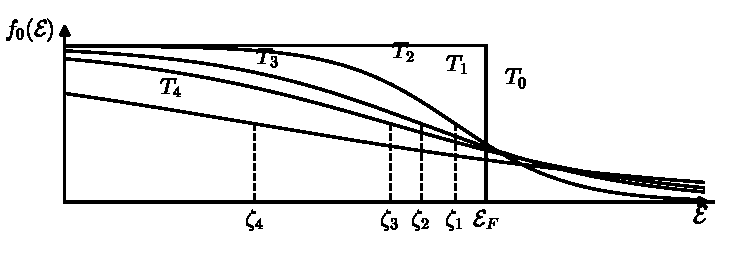
\includegraphics[width=0.72\textwidth]{fig_82.pdf}
\caption*{图 82\quad 高温下，费米–狄拉克 函数变为经典 Boltzmann 分布。}
\end{figure}

我们注意到 $\zeta<\mathcal{E}_F$，只有 $T=0$ 时例外——但当 $kT\ll\mathcal{E}_F$ 时，例如常温下的金属，这一修正很小。随着温度升高，$\zeta$ 的值不得不下降，因为 费米–狄拉克 函数在电子气的简并温度（degeneracy temperature）以上——即当 $kT>\mathcal{E}_F$ 时——必须趋于经典分布
\begin{equation*}
f^0(\mathcal{E})\propto e^{-\mathcal{E}/kT}
\tag{4.24}
\end{equation*}
从式 (4.8) 的形式显然可见，这只对 $\zeta$ 以上的能量才成立；若要它对带中所有能量都成立，$\zeta$ 的值就必须位于 $\mathcal{E}=0$ 之下。

\section{半导体中载流子的统计}

在半导体中，态密度函数有一个很大的间隙。实际上，能量的积分范围被分成两段——一段到价带（valence band）顶 $\mathcal{E}_v$ 为止，另一段从导带（conduction band）底 $\mathcal{E}_c$ 起继续向上。于是，与式 (4.9) 和式 (4.10) 相当的条件是
\begin{equation*}
\int_0^{\mathcal{E}_v} \mathcal{N}(\mathcal{E})\,d\mathcal{E} = \int_0^{\mathcal{E}_v} f^0(\mathcal{E})\mathcal{N}_v(\mathcal{E})\,d\mathcal{E} + \int_{\mathcal{E}_c}^{\infty} f^0(\mathcal{E})\mathcal{N}_c(\mathcal{E})\,d\mathcal{E},
\tag{4.25}
\end{equation*}
其中 $\mathcal{N}_c(\mathcal{E})$ 与 $\mathcal{N}_v(\mathcal{E})$ 分别是导带与价带中的态密度。

我们可以把它写成
\begin{equation*}
\int_0^{\mathcal{E}_v} \{1-f^0(\mathcal{E})\}\mathcal{N}_v(\mathcal{E})\,d\mathcal{E} = \int_{\mathcal{E}_c}^{\infty} f^0(\mathcal{E})\mathcal{N}_c(\mathcal{E})\,d\mathcal{E},
\tag{4.26}
\end{equation*}
这不过是说，被激发到导带中的电子数等于价带中留下的空穴（hole）数：
\begin{equation*}
n_h = n_e.
\tag{4.27}
\end{equation*}

式 (4.26) 中的统计函数可以改写成一种有趣的形式。让我们注意
\begin{align*}
1-f^0(\mathcal{E}-\zeta) &= 1 - \frac{1}{\exp\{(\mathcal{E}-\zeta)/kT\}+1} \\
&= \frac{1}{\exp\{-(\mathcal{E}-\zeta)/kT\}+1} \\
&= f^0(\mathcal{E}_h+\zeta_h),
\tag{4.28}
\end{align*}
其中
\begin{equation*}
\mathcal{E}_h+\zeta_h = -(\mathcal{E}-\zeta).
\tag{4.29}
\end{equation*}

换言之，在电子的费米能级（Fermi level）之下距离 $|\mathcal{E}-\zeta|$ 处的能级 $\mathcal{E}$ 上找到一个空穴的概率，与在费米能级之上距离 $|\mathcal{E}-\zeta|$ 处找到一个电子的概率相同。空穴与电子一样遵从 费米–狄拉克 统计——只不过仿佛它们的能量是\emph{向下}量的。为方便起见，我们把所有电子能量都从 $\mathcal{E}_c$ 量起；用变量 $\mathcal{E}_e$ 表示 $\mathcal{E}-\mathcal{E}_c$。空穴能量则从价带顶量起：$\mathcal{E}_h=-(\mathcal{E}-\mathcal{E}_v)$。电子的费米能级位于某一点 $\mathcal{E}_e=-\zeta_e$ 处；空穴的费米能级则相应于 $\mathcal{E}_h=-\zeta_h$。于是我们的公式 (4.26) 便读作
\begin{equation*}
\int_0^{\infty} f^0(\mathcal{E}_h+\zeta_h)\mathcal{N}_v(\mathcal{E}_h)\,d\mathcal{E}_h = \int_0^{\infty} f^0(\mathcal{E}_e+\zeta_e)\mathcal{N}_c(\mathcal{E}_e)\,d\mathcal{E}_e.
\tag{4.30}
\end{equation*}

这两个函数还须满足的进一步条件是：$\zeta_e$ 与 $\zeta_h$ 事实上应当对应于同一个总的费米势（over-all Fermi potential）$\zeta$。既然它们是从彼此相距 $\mathcal{E}_{\mathrm{gap}}$ 的能量原点分别量起的，我们便有\footnote{这里看来最方便的做法，是把 $\zeta_e$ 和 $\zeta_h$ 定义成通常均为正的量。}
\begin{equation*}
\zeta_e+\zeta_h = \mathcal{E}_{\mathrm{gap}}.
\tag{4.31}
\end{equation*}

正如我们马上就要证明的，$\zeta$ 倾向于落在间隙之中，因此 $\zeta_e$ 与 $\zeta_h$ 都是正的，而且比 $kT$ 大得多。于是，在 $\mathcal{E}_e$ 与 $\mathcal{E}_h$ 为正的范围内，电子和空穴的 Fermi 函数实际上已无法与经典分布区分：
\begin{equation*}
f^0(\mathcal{E}_e+\zeta_e) \approx \exp\{-(\mathcal{E}_e+\zeta_e)/kT\}.
\tag{4.32}
\end{equation*}

\begin{figure}[H]
\centering
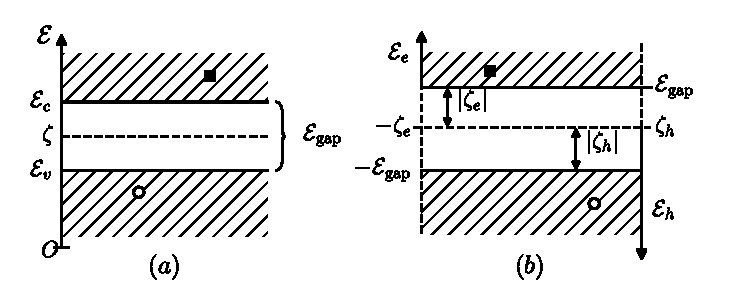
\includegraphics[width=0.72\textwidth]{fig_83.pdf}
\caption*{图 83\quad (a) 半导体的绝对能量图式。(b) “电子”与“空穴”能量图式。}
\end{figure}

这在一定程度上简化了式 (4.30) 中积分的计算。按照 van Hove 定理（§2.5），导带底附近态密度的形式必定是
\begin{equation*}
\mathcal{N}_c(\mathcal{E}_e) = \frac{1}{2\pi^2}\left(\frac{2m_e}{\hbar^2}\right)^{3/2}\mathcal{E}_e^{1/2}.
\tag{4.33}
\end{equation*}
这实际上就是\emph{有效质量}（effective mass）为 $m_e$ 的自由电子气的结果，但一般说来这个参量是
\begin{equation*}
m_e = (m_1 m_2 m_3)^{1/2},
\tag{4.34}
\end{equation*}
其中 $m_1$、$m_2$、$m_3$ 是在 $\mathbf{k}$ 空间中围绕 $\mathcal{E}(\mathbf{k})$ 的极小值、以局部主轴为参照展开能量时的展开系数：
\begin{equation*}
\mathcal{E}_e = \frac{\hbar^2 k_1^2}{2m_1} + \frac{\hbar^2 k_2^2}{2m_2} + \frac{\hbar^2 k_3^2}{2m_3}.
\tag{4.35}
\end{equation*}
其证明与式 (2.70)–(2.72) 完全相同。

把式 (4.32) 与式 (4.33) 代入 (4.30)，我们得到
\begin{align*}
n_e &= \int_0^{\infty} \exp\{-(\mathcal{E}_e+\zeta_e)/kT\}\,\frac{1}{2\pi^2}\left(\frac{2m_e}{\hbar^2}\right)^{3/2}\mathcal{E}_e^{1/2}\,d\mathcal{E}_e \\
&= \frac{1}{2\pi^2}\left(\frac{2m_e}{\hbar^2}\right)^{3/2} e^{-\zeta_e/kT}(kT)^{3/2}\int_0^{\infty} e^{-z}z^{1/2}\,dz \\
&= 2\left(\frac{m_e kT}{2\pi\hbar^2}\right)^{3/2} e^{-\zeta_e/kT}.
\tag{4.36}
\end{align*}

在简单的模型中——例如忽略自旋–轨道分裂（§3.11）时——价带顶也将具有与式 (4.33) 相同函数形式的态密度，只是改由一个具有质量量纲的类似参量 $m_h$ 刻画。对于“在温度 $T$ 下激发的空穴”的总数，将有类似的公式：
\begin{equation*}
n_h = 2\left(\frac{m_h kT}{2\pi\hbar^2}\right)^{3/2} e^{-\zeta_h/kT},
\tag{4.37}
\end{equation*}

令 $n_e$ 与 $n_h$ 相等，并利用 (4.31)，就可以把二者分别求出。例如，将 (4.36) 与 (4.37) 相乘，得
\begin{equation*}
n_e n_h = 4\left(\frac{kT}{2\pi\hbar^2}\right)^3 (m_e m_h)^{3/2} e^{-\mathcal{E}_{\mathrm{gap}}/kT},
\tag{4.38}
\end{equation*}
此式与费米能级的位置无关，因此只要费米能级保持在带隙之内，它就相当普遍地成立。对此式取平方根，得
\begin{equation*}
n_e = n_h = 2\left(\frac{kT}{2\pi\hbar^2}\right)^{3/2}(m_e m_h)^{3/4} e^{-\mathcal{E}_{\mathrm{gap}}/2kT},
\tag{4.39}
\end{equation*}
这表明载流子（carrier）密度确实按 Boltzmann 因子变化，就好像需要能量 $\frac{1}{2}\mathcal{E}_{\mathrm{gap}}$ 才能把一个电子激活到导带中去。

由 (4.36)、(4.37) 和 (4.39)，容易分别算出 $\zeta_e$ 与 $\zeta_h$；由对称性显然可知，若 $m_e=m_h$，$\zeta$ 将落在间隙正中。只要 $\mathcal{E}_g\gg kT$，这些公式就对载流子全部由热激发产生的\emph{本征半导体}（intrinsic semiconductor）成立。

在本书中，我们把讨论主要限于纯净、有序的固体；但应当提到，大多数半导体并不很纯——实际上，我们几乎总是在掺入杂质、经过\emph{掺杂}（doped）的状态下使用它们。标准的情形是\emph{施主}（donor）杂质——一个以替位方式掺入 Ge 晶体的 As 原子。由 §4.2 的论证显然可知，只要让 As 的第 5 个电子被释放到晶体的导带之中，这种替换就可以在不损害晶格键结构的情况下实现。这样我们便制得一个 \emph{n 型}（n-type）样品；我们增加了几个电子，却没有在价带中产生任何空穴。

若每单位体积中有 $N_d$ 个这样的\emph{施主原子}，则必有
\begin{equation*}
n_e - n_h = N_d
\tag{4.40}
\end{equation*}
以此作为条件，从中求出 $n_e$、$n_h$、$\zeta_e$、$\zeta_h$ 随 $T$ 变化的函数关系。特别是，若通过添加大量施主使材料重度掺杂，电子将占压倒性的优势。这时费米能级必定落在这些\emph{多数载流子}（majority carriers）所占据的能量范围内——即靠近导带底。掺杂足够多时，这种载流子气可以达到金属的密度，从而即使在常温下分布也变成简并的。

\begin{figure}[H]
\centering
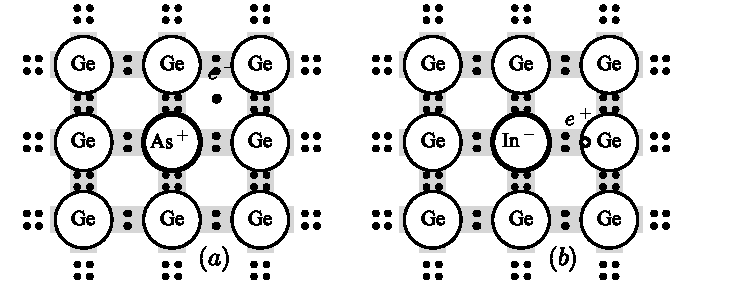
\includegraphics[width=0.72\textwidth]{fig_84.pdf}
\caption*{图 84\quad (a) Ge 中的施主。(b) Ge 中的受主。}
\end{figure}

这类杂质还有一种对偶的情形。如果我们用 In——每个原子只有 3 个电子——来代替 Ge，键就不能完全填满；价带中留下一个空穴。晶体中密度为 $N_a$ 的\emph{受主}（acceptor）杂质造成一个 \emph{p 型}（p-type）样品，其中
\begin{equation*}
n_e - n_h = -N_a.
\tag{4.41}
\end{equation*}

一般地，施主与受主可能同时存在，于是在\emph{补偿}（compensated）样品中有
\begin{equation*}
n_e - n_h = N_d - N_a.
\tag{4.42}
\end{equation*}
不过，这些杂质也会把局域的杂质能级引入能隙之中（见 §6.4）；因此，当温度低到这些能级可能被相当大比例的过剩载流子占据时，统计理论就变得更复杂了。

\section{电子比热}

金属中的电子必然对比热有所贡献。为了计算这一贡献，让我们利用式 (4.21) 计算电子分布的平均能量，因为我们假定系统是高度简并的：
\begin{align*}
\overline{\mathcal{E}} &= \int \mathcal{E}f^0(\mathcal{E})\mathcal{N}(\mathcal{E})\,d\mathcal{E} \\
&= \int_0^{\zeta} \mathcal{E}\mathcal{N}(\mathcal{E})\,d\mathcal{E} + \frac{\pi^2}{6}(kT)^2\left[\frac{\partial}{\partial \mathcal{E}}\{\mathcal{E}\mathcal{N}(\mathcal{E})\}\right]_{\mathcal{E}=\zeta} + \ldots.
\tag{4.43}
\end{align*}

我们对温度求微商，同时注意到（参见式 (4.22)）$\zeta$ 是 $T$ 的函数：
\begin{align*}
C_{\mathrm{el.}} &= \frac{\partial \overline{\mathcal{E}}}{\partial T} = \zeta\mathcal{N}(\zeta)\frac{d\zeta}{dT} + \frac{\pi^2}{3}k^2T\left[\mathcal{N}(\mathcal{E}) + \zeta\frac{\partial \mathcal{N}(\mathcal{E})}{\partial \mathcal{E}}\right]_{\mathcal{E}=\zeta} + O(T^2) \\
&= \frac{\pi^2}{3}k^2T\mathcal{N}(\mathcal{E}_F) + \zeta\mathcal{N}(\zeta)\left[\frac{d\zeta}{dT} + \frac{\pi^2}{3}\frac{k^2T}{\mathcal{N}(\mathcal{E})}\frac{\partial \mathcal{N}(\mathcal{E})}{\partial \mathcal{E}}\right]_{\mathcal{E}=\zeta} \\
&= nk\,\frac{\pi^2}{3}kT\,\frac{\mathcal{N}(\mathcal{E}_F)}{n}
\tag{4.44}
\end{align*}
其中最后一步由式 (4.22) 得出。$T^2$ 等更高阶的项都可以忽略。

这是一个十分重要的结果。把式 (4.44) 与经典粒子气体的比热——譬如说 $\frac{3}{2}nk$——作一比较，量子结果要小得多。对自由电子，态密度式 (4.3) 为 $\frac{3}{2}n/\mathcal{E}_F$，于是
\begin{equation*}
C_{\mathrm{el.}}/C_{\mathrm{classical}} = \frac{\pi^2}{3}\frac{kT}{\mathcal{E}_F}.
\tag{4.45}
\end{equation*}
在普通金属中、普通温度下，这个因子约为 $1/100$。它说明了为什么金属的总比热可以由 §2.4 的晶格项相当准确地给出，也说明了为什么 Dulong–Petit 定律在高温下成立。

我们还注意到 $C_{\mathrm{el.}}$ 与 $T$ 成线性。在极低温度下，这一线性项——通常写作
\begin{equation*}
C_{\mathrm{el.}} = \gamma T,
\tag{4.46}
\end{equation*}
——可以与晶格项区分开来，后者按 $T^3$ 更快地趋于零。测量 $\gamma$ 可以直接给出关于 $\mathcal{N}(\mathcal{E}_F)$——费米能级处的态密度——的信息。例如，在过渡金属中观察到很大的 $\gamma$ 值，正如 §4.4 中所讨论的。

我们可以这样理解这条线性定律。看看 费米分布（图 85）；温度的作用是使少数电子被激发到更高的能级。但这一效应只在 $\mathcal{E}_F$ 附近 $kT$ 量级的能量范围内才是明显的。我们可以说，大约有 $kT\,\mathcal{N}(\mathcal{E}_F)$ 个电子各获得约 $kT$ 的能量。于是，整个固体获得的能量为
\begin{equation*}
\delta\overline{\mathcal{E}} \sim k^2T^2\mathcal{N}(\mathcal{E}_F).
\tag{4.47}
\end{equation*}
与此相应，
\begin{equation*}
C_{\mathrm{el.}} = \frac{\partial \delta\overline{\mathcal{E}}}{\partial T} \sim 2k^2T\mathcal{N}(\mathcal{E}_F).
\tag{4.48}
\end{equation*}
除一个数值因子外，这基本上就是我们的结果 (4.44)。

\begin{figure}[H]
\centering
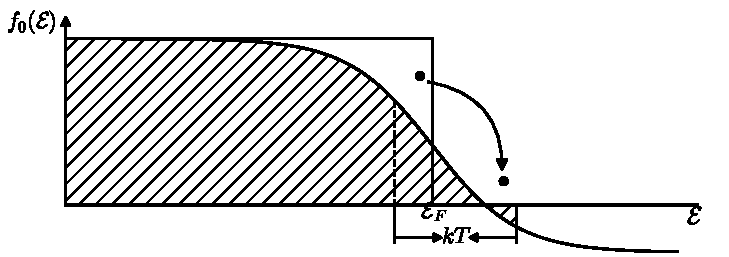
\includegraphics[width=0.72\textwidth]{fig_85.pdf}
\caption*{图 85\quad 金属中电子的热激发。}
\end{figure}

实际上，我们要说的是：处在分布深处的电子几乎觉察不到温度的存在。它们的处境由 Pauli 原理决定；这一原理坚持要它们填满所有的能级，却不允许它们侵占彼此的状态。这并不比下面这件事更令人奇怪：离子实束缚态深处的电子不必算作对固体比热的一种单独贡献——至少在温度还没有高到足以把这些电子热激发起来之前是如此。

 % 本文件由 scripts/assemble.py 自动装配，勿手改（改 parts/ 后重跑）
% 第5章 电子间相互作用

% 第5章 Electron–Electron Interaction
\chapter{电子间相互作用}

\epigraphbook{“这整个事情就是一个糊弄我们高贵轻信的低劣骗局”\\——Sam 说}{NORMAN LINDSAY，\emph{The Magic Pudding}}

\section{微扰表述}

第 3 章所讲述的电子结构理论是一种\emph{单电子模型}（one-electron model）：每个电子都被当作一个独立的粒子，在一个完全确定的势中运动，而传导电子之间的相互作用则被略去。但我们知道，这些相互作用是强的，而且是长程的——它们就是电荷之间的库仑力（Coulomb force），以及与波函数的反对称性相联系的所谓交换力（exchange force）。

我们天真地假定，这些相互作用可以靠一次 Hartree 或 Hartree--Fock 自洽计算来料理妥当：这种计算按照价电子的电荷分布（当然，也包括离子实各闭壳层中的电子）来调整原子势。但要把这件事做得妥当并不容易——我们也许不得不退而依靠某种假设，例如 Wigner 和 Seitz（§4.3）所用的那一个：电子看到的是它恰好置身其中的那个晶胞里一个带单电荷的离子的势，而相邻的晶胞则是电中性的。

因此，近年来人们在一团经由各自库仑势相互作用的电子气的这个\emph{多体问题}（many-body problem）上耗费了大量精力，如今相互作用的基本效应已被理解得相当清楚。这理论的许多部分是用复杂的形式语言表述的；其主要结果却出人意料地简单，而且可以用初等的论证推导出来。

我们考虑一个自由电子气，它受到一个随时间变化的微扰。设在时刻 $t$、位于 $\mathbf{r}$ 处的电子感受到的势为
\begin{equation*}
\delta\mathcal{U}(\mathbf{r},t)=\mathcal{U}\,e^{i\mathbf{q}\cdot\mathbf{r}}e^{i\omega t}e^{\alpha t}.
\tag{5.1}
\end{equation*}
我们施加了一个频率为 $\omega$、波矢为 $\mathbf{q}$ 的振荡，它以时间常数 $\alpha$ 缓慢增长。

作用在态 $|\mathbf{k}\rangle=\exp i\{\mathbf{k}\cdot\mathbf{r}+\mathcal{E}(\mathbf{k})t/\hbar\}$ 上时，它把别的态混入进来，于是波函数变成
\begin{equation*}
\psi_{\mathbf{k}}(\mathbf{r},t)=|\mathbf{k}\rangle+b_{\mathbf{k}+\mathbf{q}}(t)\,|\mathbf{k}+\mathbf{q}\rangle,
\tag{5.2}
\end{equation*}
其中系数可以用微扰论算到一级：
\begin{align*}
b_{\mathbf{k}+\mathbf{q}}(t)&=\frac{\langle\mathbf{k}+\mathbf{q}\,|\,\delta\mathcal{U}\,|\,\mathbf{k}\rangle}{\mathcal{E}(\mathbf{k})-\mathcal{E}(\mathbf{k}+\mathbf{q})+\hbar\omega-i\hbar\alpha}\\
&=\frac{\mathcal{U}\,e^{i\omega t}e^{\alpha t}}{\mathcal{E}(\mathbf{k})-\mathcal{E}(\mathbf{k}+\mathbf{q})+\hbar\omega-i\hbar\alpha}.
\tag{5.3}
\end{align*}
这可以直接由 $\psi_{\mathbf{k}}$ 的含时 Schrödinger 方程看出：未微扰的哈密顿量——正好就是动能算符，其本征值为 $\mathcal{E}(\mathbf{k})$——被式 (5.1) 所增广，而式 (5.1) 被认为是小的。

现在考虑电子波函数的这一变化所引起的电荷密度的改变。我们假定所处理的是\emph{凝胶}（jellium），即电子在其上运动的一种均匀带正电的介质。
\begin{align*}
\delta\rho(\mathbf{r},t)&=e\sum_{\mathbf{k}}\left\{\left|\psi_{\mathbf{k}}(\mathbf{r},t)\right|^{2}-1\right\}\\
&=e\sum_{\mathbf{k}}\left[\left\{e^{-i\mathbf{k}\cdot\mathbf{r}}+b_{\mathbf{k}+\mathbf{q}}^{*}(t)\,e^{-i(\mathbf{k}+\mathbf{q})\cdot\mathbf{r}}\right\}\left\{e^{i\mathbf{k}\cdot\mathbf{r}}+b_{\mathbf{k}+\mathbf{q}}(t)\,e^{i(\mathbf{k}+\mathbf{q})\cdot\mathbf{r}}\right\}-1\right]\\
&\approx e\sum_{\mathbf{k}}\left\{b_{\mathbf{k}+\mathbf{q}}(t)\,e^{i\mathbf{q}\cdot\mathbf{r}}+b_{\mathbf{k}+\mathbf{q}}^{*}(t)\,e^{-i\mathbf{q}\cdot\mathbf{r}}\right\},
\tag{5.4}
\end{align*}
这里是舍去了 $|b|^{2}$ 项的结果。此处的求和遍及所有被占据的电子态。

由于 $\delta\rho$ 按其定义是实的，我们发现波 (5.1) 产生两类电荷扰动：一类随波一同行进，另一类则与波有 $180^{\circ}$ 的相位差。如果我们假定实际上遇到的是实微扰，也就是说，如果在 (5.1) 上加上它的复共轭
\begin{equation*}
\delta\mathcal{U}^{*}(\mathbf{r},t)=\mathcal{U}\,e^{-i\mathbf{q}\cdot\mathbf{r}}e^{-i\omega t}e^{\alpha t},
\tag{5.5}
\end{equation*}
那么我们发现电荷密度的变化就跟随总微扰，而不引入任何额外的 Fourier 分量，即
\begin{align*}
\delta\rho=e\sum_{\mathbf{k}}\bigg\{&\frac{\mathcal{U}}{\mathcal{E}(\mathbf{k})-\mathcal{E}(\mathbf{k}+\mathbf{q})+\hbar\omega-i\hbar\alpha}\\
&+\frac{\mathcal{U}}{\mathcal{E}(\mathbf{k})-\mathcal{E}(\mathbf{k}-\mathbf{q})-\hbar\omega+i\hbar\alpha}\bigg\}e^{i\mathbf{q}\cdot\mathbf{r}}e^{i\omega t}e^{\alpha t}+\text{复共轭}.
\tag{5.6}
\end{align*}

为了把这一点弄得稍微更一般些，让我们引入 $f_{0}(\mathbf{k})$，作为未微扰金属中 $|\mathbf{k}\rangle$ 被占据的概率——例如它可以是费米--狄拉克（Fermi--Dirac）函数 (4.8)。在 (5.6) 的第二项中把标记 $\mathbf{k}$ 换写成 $\mathbf{k}-\mathbf{q}$，我们便可以把求和写成如下形式
\begin{equation*}
\delta\rho=e\mathcal{U}\sum_{\mathbf{k}}\left\{\frac{f^{0}(\mathbf{k})-f^{0}(\mathbf{k}+\mathbf{q})}{\mathcal{E}(\mathbf{k})-\mathcal{E}(\mathbf{k}+\mathbf{q})+\hbar\omega-i\hbar\alpha}\right\}e^{i\mathbf{q}\cdot\mathbf{r}}e^{i\omega t}e^{\alpha t}+\text{复共轭},
\tag{5.7}
\end{equation*}
其中求和现在遍及所有态 $|\mathbf{k}\rangle$，无论“被占据的”还是“未被占据的”。

这一电荷分布经由库仑相互作用产生一个作用于电子的势能场。若把它记作 $\delta\Phi(\mathbf{r},t)$，则按泊松（Poisson）方程必有
\begin{equation*}
\nabla^{2}(\delta\Phi)=-4\pi e\,\delta\rho.
\tag{5.8}
\end{equation*}
我们可以假定 $\delta\Phi$ 与 $\delta\rho$ 具有同样的空间和时间变化，即写成
\begin{equation*}
\delta\Phi(\mathbf{r},t)=\Phi\,e^{i\mathbf{q}\cdot\mathbf{r}}e^{i\omega t}e^{\alpha t}+\text{复共轭}.
\tag{5.9}
\end{equation*}
把 (5.7)、(5.8) 与 (5.9) 联立，便得
\begin{equation*}
-q^{2}\Phi=-4\pi e^{2}\mathcal{U}\sum_{\mathbf{k}}\frac{f^{0}(\mathbf{k})-f^{0}(\mathbf{k}+\mathbf{q})}{\mathcal{E}(\mathbf{k})-\mathcal{E}(\mathbf{k}+\mathbf{q})+\hbar\omega-i\hbar\alpha},
\tag{5.10}
\end{equation*}
即
\begin{equation*}
\Phi=\left\{\frac{4\pi e^{2}}{q^{2}}\sum_{\mathbf{k}}\frac{f^{0}(\mathbf{k})-f^{0}(\mathbf{k}+\mathbf{q})}{\mathcal{E}(\mathbf{k})-\mathcal{E}(\mathbf{k}+\mathbf{q})+\hbar\omega-i\hbar\alpha}\right\}\mathcal{U}.
\tag{5.11}
\end{equation*}

这就是与原来的势 $\delta\mathcal{U}$ 所感生的电荷重新分布相联系的势（能）。但这个新的势 $\delta\Phi$ 其实本来就应该被算作电子分布所受微扰的一部分。为了使计算自洽，我们所假设的微扰 $\delta\mathcal{U}$ 本应已经把 $\delta\Phi$ 包含在内。换言之
\begin{equation*}
\delta\mathcal{U}(\mathbf{r},t)=\delta\mathcal{V}(\mathbf{r},t)+\delta\Phi(\mathbf{r},t),
\tag{5.12}
\end{equation*}
其中 $\delta\mathcal{V}(\mathbf{r},t)$ 是我们自以为施加了的那个真实外势。

如果我们假定 $\delta\mathcal{V}$ 具有如下形式
\begin{equation*}
\delta\mathcal{V}=\mathcal{V}\,e^{i\mathbf{q}\cdot\mathbf{r}}e^{i\omega t}e^{\alpha t}+\text{复共轭},
\tag{5.13}
\end{equation*}
那么由 (5.12) 和 (5.11) 得
\begin{equation*}
\mathcal{U}=\mathcal{V}+\left\{\frac{4\pi e^{2}}{q^{2}}\sum_{\mathbf{k}}\frac{f^{0}(\mathbf{k})-f^{0}(\mathbf{k}+\mathbf{q})}{\mathcal{E}(\mathbf{k})-\mathcal{E}(\mathbf{k}+\mathbf{q})+\hbar\omega-i\hbar\alpha}\right\}\mathcal{U}
\tag{5.14}
\end{equation*}
或
\begin{equation*}
\mathcal{U}=\frac{\mathcal{V}}{\epsilon(\mathbf{q},\omega)},
\tag{5.15}
\end{equation*}
其中
\begin{equation*}
\epsilon(\mathbf{q},\omega)\equiv 1+\frac{4\pi e^{2}}{q^{2}}\sum_{\mathbf{k}}\frac{f^{0}(\mathbf{k})-f^{0}(\mathbf{k}+\mathbf{q})}{\mathcal{E}(\mathbf{k}+\mathbf{q})-\mathcal{E}(\mathbf{k})-\hbar\omega+i\hbar\alpha}
\tag{5.16}
\end{equation*}
（求和中分母的正负号是为了方便而作了更换）。

换句话说，作用于电子的有效势 $\mathcal{U}$ 并不是外加的势 $\mathcal{V}$，而是要除以一个\emph{介电常数}（dielectric constant）$\epsilon(\mathbf{q},\omega)$；它是外加微扰的波长和频率的函数。我们是对单个 Fourier 分量导出这个结果的，但由于我们在 (5.2)、(5.4) 等处已把方程线性化，所以可以把不同 Fourier 分量的效应加起来。于是，若把 $\delta\mathcal{V}$ 用 Fourier 积分表示为
\begin{equation*}
\delta\mathcal{V}(\mathbf{r},t)=\iint\mathcal{V}(\mathbf{q},\omega)\,e^{i\mathbf{q}\cdot\mathbf{r}}e^{i\omega t}\,\mathrm{d}\mathbf{q}\,\mathrm{d}\omega,
\tag{5.17}
\end{equation*}
就可以由下式算出电子所感受到的有效势：
\begin{equation*}
\delta\mathcal{U}(\mathbf{r},t)=\iint\frac{\mathcal{V}(\mathbf{q},\omega)}{\epsilon(\mathbf{q},\omega)}\,e^{i\mathbf{q}\cdot\mathbf{r}}e^{i\omega t}\,\mathrm{d}\mathbf{q}\,\mathrm{d}\omega.
\tag{5.18}
\end{equation*}

公式 (5.16) 被称为 \emph{Lindhard 表达式}（Lindhard's expression）。在本章下面几节中我们将证明，它孕育着对一系列物理现象的种种富有成果的描述的种子。

\section{静态屏蔽}

让我们考虑 $\omega=0$ 的静态微扰的效应。先考察 $\epsilon(\mathbf{q},0)$ 在 $q=0$ 附近的形式。在 (5.16) 中我们可以近似地写
\begin{equation*}
\mathcal{E}(\mathbf{k}+\mathbf{q})-\mathcal{E}(\mathbf{k})\approx\mathbf{q}\cdot\nabla_{\mathbf{k}}\mathcal{E}(\mathbf{k})
\tag{5.19}
\end{equation*}
并且，注意到 $f^{0}(\mathbf{k})$ 只是 $\mathcal{E}(\mathbf{k})$ 的函数，
\begin{equation*}
f^{0}(\mathbf{k})-f^{0}(\mathbf{k}+\mathbf{q})\approx-\mathbf{q}\cdot\frac{\partial f^{0}}{\partial\mathcal{E}}\,\nabla_{\mathbf{k}}\mathcal{E}(\mathbf{k}).
\tag{5.20}
\end{equation*}

(5.16) 中的求和可以写成一个积分（记住，原则上它现在遍及所有态，既包括占据的也包括空的）：
\begin{align*}
\epsilon(\mathbf{q},0)&\to 1+\frac{4\pi e^{2}}{q^{2}}\int\frac{\left\{\mathbf{q}\cdot\nabla_{\mathbf{k}}\mathcal{E}(\mathbf{k})\right\}}{\left\{\mathbf{q}\cdot\nabla_{\mathbf{k}}\mathcal{E}(\mathbf{k})\right\}}\left(-\frac{\partial f^{0}}{\partial\mathcal{E}}\right)\mathrm{d}\mathbf{k}\\
&=1+\frac{4\pi e^{2}}{q^{2}}\int\left(-\frac{\partial f^{0}}{\partial\mathcal{E}}\right)\mathcal{N}(\mathcal{E})\,\mathrm{d}\mathcal{E}\\
&=1+\frac{\lambda^{2}}{q^{2}},
\tag{5.21}
\end{align*}
其中
\begin{equation*}
\lambda^{2}=4\pi e^{2}\mathcal{N}(\mathcal{E}_{F})
\tag{5.22}
\end{equation*}
因为 $\left(-\partial f^{0}/\partial\mathcal{E}\right)$ 只是能量的函数，而且按 (4.13)--(4.18)，它实际上就是费米能级处的一个 $\delta$ 函数。

这个结果表明，当 $q\to 0$ 时 $\epsilon\to\infty$。看一眼 (5.15) 便知，这意味着对固定的 $\mathcal{V}$，当 $q\to 0$ 时 $\mathcal{U}\to 0$。换言之，\emph{长波长的外场几乎完全被电子的流动所屏蔽}。

用更初等的论证——在 Thomas--Fermi 近似中——也能得到同样的结果。设在某点 $\mathbf{r}$ 处有一个微扰势 $\delta\mathcal{U}$。于是电子的费米分布将相对于 $\delta\mathcal{U}$ 为零之处的分布被抬高这一数量。但这意味着，除非电子从这一区域流走，否则费米能级 $\zeta$ 就会改变。事实上这必定发生，因为 $\zeta$ 作为化学势，在整个体积内处处相同。

\begin{figure}[H]
\centering
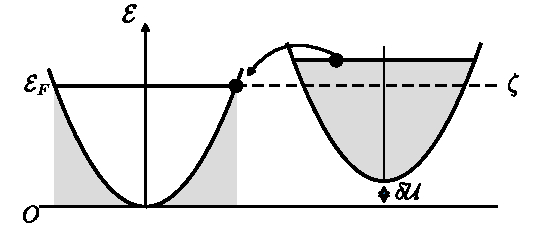
\includegraphics[width=0.72\textwidth]{fig_86.pdf}
\caption*{图 86\quad 微扰对费米分布的效应。}
\end{figure}

如果 $\delta\mathcal{U}$ 很小，我们就从分布的顶部削去这样厚的一层；也就是说，局域电子密度改变了
\begin{equation*}
\delta n(\mathbf{r})=-\mathcal{N}(\mathcal{E}_{F})\,\delta\mathcal{U}(\mathbf{r}).
\tag{5.23}
\end{equation*}
但电子密度的改变对应于局域电荷密度的改变，而后者又转而产生一个势 $\delta\Phi(\mathbf{r})$。它必须满足泊松方程
\begin{align*}
\nabla^{2}(\delta\Phi)&=-4\pi e^{2}\,\delta n(\mathbf{r})\\
&=4\pi e^{2}\mathcal{N}(\mathcal{E}_{F})\,\delta\mathcal{U}(\mathbf{r})\\
&=\lambda^{2}\delta\mathcal{U}.
\tag{5.24}
\end{align*}
这就是 (5.11) 在作 Fourier 变换之前的等价形式，只是用 $\mathcal{N}(\mathcal{E}_{F})$ 代替了对 $\mathbf{k}$ 的求和：我们便回到了 (5.21)。

注意，对\emph{经典气体}（classical gas）——例如半导体中的载流子——我们可以论证 (5.23) 应当代之以下式
\begin{align*}
\delta n(\mathbf{r})&\approx n_{0}\exp\left\{-\delta\mathcal{U}(\mathbf{r})/kT\right\}-n_{0}\\
&\approx-\frac{n_{0}}{kT}\,\delta\mathcal{U},
\tag{5.25}
\end{align*}
其中 $n_{0}$ 是载流子的局域平均密度。这可以由 (4.32) 之类的公式得到。我们得到与 (5.24) 同类型的公式，只是现在
\begin{equation*}
\lambda^{2}=\frac{4\pi e^{2}n_{0}}{kT}.
\tag{5.26}
\end{equation*}
自由电子气的态密度可以写成
\begin{equation*}
\mathcal{N}(\mathcal{E}_{F})=\frac{3}{2}\,\frac{n}{kT_{F}},
\tag{5.27}
\end{equation*}
其中 $T_{F}$ 是气体的\emph{费米温度}（Fermi temperature）（即 $\mathcal{E}_{F}/k$）。于是，\emph{屏蔽参数}（screening parameter）$\lambda$ 的量子理论公式 (5.22) 在“电子具有非常高的有效温度 $\sim T_{F}$”这一假设之下，就等价于经典的 \emph{Debye--Hückel 公式} (5.26)。在 (5.21) 的推导中直接取 $f^{0}$ 为 Boltzmann 分布，同样可以直接得到 (5.26)。

\section{被屏蔽的杂质与中性赝原子}

固体中微扰场的一个典型例子是带电杂质周围的静电场。如果在金属晶格中用一个 Zn 离子替换一个 Cu 离子，我们就在原先只有一个电荷的地方放进了电荷 $+2|e|$。我们把这一杂质当作中性背景中一个净电荷 $+|e|$ 来处理，并计算它对自由电子气的效应。

计算这个问题最简单的办法，是在 (5.24) 中假定 $\delta\mathcal{U}$ 和 $\delta\Phi$ 相同，只是杂质的最中心处除外。方程
\begin{equation*}
\nabla^{2}(\delta\mathcal{U})=\lambda^{2}(\delta\mathcal{U})
\tag{5.28}
\end{equation*}
具有如下形式的解
\begin{equation*}
\delta\mathcal{U}=\frac{e^{2}}{r}\exp(-\lambda r),
\tag{5.29}
\end{equation*}
其中我们让势在 $r=0$ 附近表现得如同点电荷的势。这是一个典型的结果：我们得到一个\emph{被屏蔽的库仑势}（screened Coulomb potential），它随距离按指数律衰减，\emph{屏蔽半径}（screening radius）为 $1/\lambda$。按照我们的一般屏蔽原理，在这个半径的几倍之外，电子就“看不见”这个杂质了。在金属中，这个半径是原子间距的量级；在半导体中它则要大得多。

让我们从介电表述出发来得到这个结果。“外”场 $\delta\mathcal{V}(\mathbf{r})$ 是一个裸库仑势
\begin{equation*}
\delta\mathcal{V}(\mathbf{r})=\frac{e^{2}}{r}.
\tag{5.30}
\end{equation*}
这个函数在单位体积的三维盒子中的 Fourier 变换式 (5.17) 是众所周知的：
\begin{equation*}
\mathcal{V}(\mathbf{q})=\frac{4\pi e^{2}}{q^{2}}.
\tag{5.31}
\end{equation*}

\begin{figure}[H]
\centering
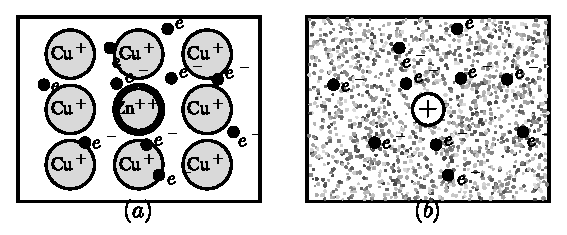
\includegraphics[width=0.72\textwidth]{fig_87.pdf}
\caption*{图 87\quad (a) 单价金属中的二价杂质换成为 (b) 连续媒质中的点电荷。}
\end{figure}

我们注意到它在 $q=0$ 处是奇异的，这正对应于库仑势的无限“程长”。

由 (5.15) 和 (5.21)，屏蔽势为
\begin{align*}
\mathcal{U}(\mathbf{q})&=\frac{4\pi e^{2}}{q^{2}\left(1+\lambda^{2}/q^{2}\right)}\\
&=\frac{4\pi e^{2}}{\lambda^{2}+q^{2}}.
\tag{5.32}
\end{align*}
众所周知，这正是我们在 (5.29) 中已经导出的势 $\delta\mathcal{U}(\mathbf{r})$ 的 Fourier 变换式 (5.18)。$\epsilon(\mathbf{q},0)$ 在 $q\to 0$ 处的奇异性抵消了 $\mathcal{V}(\mathbf{q})$ 的奇异性，从而除去了裸库仑势 (5.30) 的长程部分。

这一形式体系也可以用来处理电子--电子相互作用对纯金属中势分布的影响。原则上，我们可以算出自洽屏蔽势 $\mathcal{U}_{s}(\mathbf{r})$ 的矩阵元——诸如在 N.F.E.（近自由电子）能带结构计算（§5.3；译注：疑为 §3.3 之误印）中我们会需要的那样——办法是把裸离子势 $\mathcal{V}_{b}(r)$ 的相应 Fourier 分量除以介电函数，如 (5.18) 那样。

对于真实的深芯势，这种做法并不适用。但是，假如我们循着赝势方法的思路，用在 §3.9 中定义的模型赝势 $w_{b}(r)$ 来表示每个裸离子的场，那么，只要离子实不相互交叠，我们就可以把屏蔽之前的总“势”写成离子赝势的叠加，即
\begin{equation*}
\mathcal{V}_{b}(\mathbf{r})=\sum_{l}w_{b}(\mathbf{r}-\mathbf{R}_{l}).
\tag{5.33}
\end{equation*}
按 (2.86) 和 (5.18)，相应的自洽势具有 Fourier 分量
\begin{equation*}
\mathcal{U}_{s}(\mathbf{K})=\frac{1}{N}\sum_{l}e^{i\mathbf{K}\cdot\mathbf{R}_{l}}\,\frac{w_{b}(\mathbf{K})}{\epsilon(K,0)},
\tag{5.34}
\end{equation*}
其中现在的 $w_{b}(\mathbf{K})$ 是赝势 $w_{b}$ 的 Fourier 变换或矩阵元。在规则晶格中，结构因子 (2.92) 只不过挑出倒格矢，于是这个公式就给出了 N.F.E. 形式体系（例如 (3.64)）中系数 $\Gamma$ 的屏蔽赝势矩阵元。

适当地选取结构因子，我们还可以把 (5.34) 用作传导电子被对晶体序的偏离所散射的净矩阵元的估计——例如被声子（§6.12）散射，甚至在液态金属中也如此。在这类情形下，把这个公式改写成某个实空间函数的 Fourier 变换（与 (5.33) 类似）是有启发意义的：线性屏蔽近似使我们得以把屏蔽与叠加这两个操作互换次序，从而给出
\begin{equation*}
\mathcal{U}_{s}(\mathbf{r})\doteq\sum_{l}w_{s}(\mathbf{r}-\mathbf{R}_{l}),
\tag{5.35}
\end{equation*}
其中每个原子中心 $\mathbf{R}_{l}$ 现在似乎都携带着一个被屏蔽的离子赝势 $w_{s}(r)$，其 Fourier 变换为 $w_{b}(\mathbf{K})/\epsilon(K,0)$（图 88）。

\begin{figure}[H]
\centering
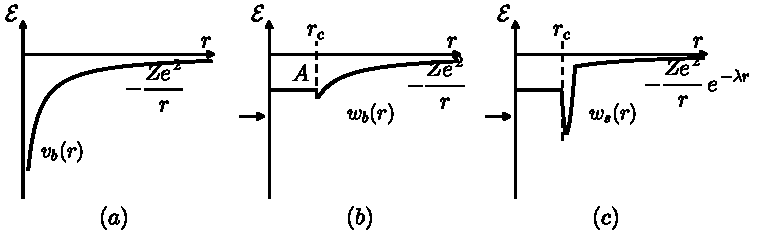
\includegraphics[width=0.72\textwidth]{fig_88.pdf}
\caption*{图 88\quad (a) 裸离子势；(b) 裸离子赝势；(c) 被屏蔽的赝势。}
\end{figure}

如我们所见，屏蔽的主要后果是把长程库仑势变成屏蔽库仑函数 (5.29)。由 (5.7) 或 (5.23)，我们不难证明，每个离子现在都携带着一团电子电荷云，其密度随距离按指数律衰减，程长为 $\lambda$（译注：按式 (5.29)，衰减的程长应为 $1/\lambda$）。从远处看，这团电荷云必定恰好含有足以中和价电荷 $+Z|e|$ 的负电荷。换言之，我们造就了一种\emph{中性赝原子}（neutral pseudo-atom），在许多金属体系中可以把它当作一个单一实体来对待。例如在热振动中（图 89），离子偏离其格点的位移产生一个电场，使电子气极化，从而引起进一步的电荷转移：在线性响应近似之内，所有这些效应都只需把赝原子作为一个整体挪动，便可自洽地计入。

\begin{figure}[H]
\centering
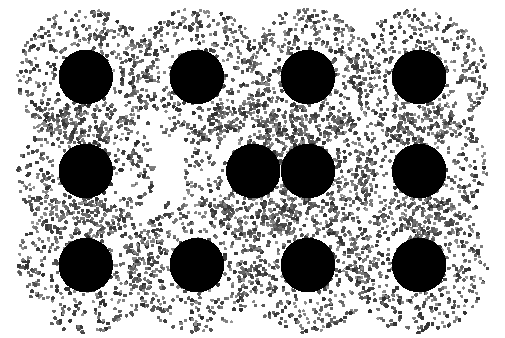
\includegraphics[width=0.72\textwidth]{fig_89.pdf}
\caption*{图 89\quad 中性赝原子。}
\end{figure}

然而要注意，相邻离子的屏蔽云必定总是相互交叠的，而且它们加起来差不多就是间隙区域中假定的自由电子密度。在真正的“原子性”聚集体（例如固态氩）中，电子定域在原子轨道上，这些轨道一旦被迫相互接触，就倾向于强烈地彼此排斥。金属中的屏蔽云无非是由传导电子气的无数\emph{非定域}（non-localized）态所贡献的\emph{平均}电荷密度的一种局域堆积而已。

赝原子方法不过是消除裸离子势在芯区深处和长程处的发散的一种近似手段。尽管如此，对于简单金属来说，它在直观上是可靠的，并且对许多可观测的量给出极好的“零级”估计（见 §§6.12、6.13）。

\section{屏蔽中的奇点：Kohn 效应}

介电常数的公式 (5.21) 只是一个近似。如果想研究短距离上的屏蔽，我们就需要对大的 $\mathbf{q}$ 值算出 (5.16) 中的和。这依赖于能量面 $\mathcal{E}(\mathbf{k})$ 的细致结构。对于绝对零度下的自由电子模型，通过对 $\mathbf{k}$ 空间作直接积分来求出这个和并不十分困难。结果如下：
\begin{equation*}
\epsilon(\mathbf{q},0)=1+\frac{4\pi e^{2}}{q^{2}}\,\frac{n}{\frac{2}{3}\mathcal{E}_{F}}\left\{\frac{1}{2}+\frac{4k_{F}^{2}-q^{2}}{8k_{F}q}\ln\left|\frac{2k_{F}+q}{2k_{F}-q}\right|\right\},
\tag{5.36}
\end{equation*}
其中 $k_{F}$ 是费米球的半径。

\begin{figure}[H]
\centering
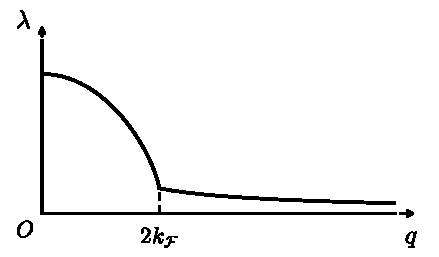
\includegraphics[width=0.72\textwidth]{fig_90.pdf}
\caption*{图 90\quad 屏蔽参数随波数的变化。}
\end{figure}

如果按 (5.21) 的形式把它写出来，那么我们看到 $\lambda$ 变成了 $q$ 的函数，当 $q\to 0$ 时趋于 (5.22)。有效屏蔽长度（effective screening length）$1/\lambda$ 随 $q$ 的增大而趋于增大。要让电子分布把短波长的势屏蔽掉，变得越来越困难。

这个公式有趣之处在于 $q=2k_{F}$ 处发生的情况，在那里对数项是奇异的。这是真实的效应。它来源于 (5.16) 中和式的形式，其中含有 $f^{0}(\mathbf{k})-f^{0}(\mathbf{k}+\mathbf{q})$。因此，我们只需考虑这样的 $\mathbf{k}$ 值：$|\mathbf{k}\rangle$ 被占据而 $|\mathbf{k}+\mathbf{q}\rangle$ 为空，或者相反。当 $q$ 小时，它们位于覆盖球面的两个区域中（图 91(a)）。随着 $q$ 增大，这些区域稳步扩张，于是和随之增大。但最终会到达这样一个 $q$ 值，此时整个球面对和都有贡献。这发生在
\begin{equation*}
q=q_{c}=2k_{F}.
\tag{5.37}
\end{equation*}

越过这一点之后，对 $\mathbf{k}$ 的求和中不再添入新项，于是和的函数形式发生改变，尽管其中每一项都仍然是 $\mathbf{q}$ 的连续函数。不过，在我们到达 $2k_{F}$ 之前球面上最后少数几个点的贡献很小，所以这个奇异性并不严重。介电函数本身保持连续，但 $\partial\epsilon/\partial q$ 在 $q=q_{c}$ 处有一个对数型的无穷大。这一论证可以推广到费米面不是球面的情形：任何具有 (5.16) 那般普遍形式之和，对于恰好张跨费米面的那些 $\mathbf{q}$ 值都会有类似的奇异性。

\begin{figure}[H]
\centering
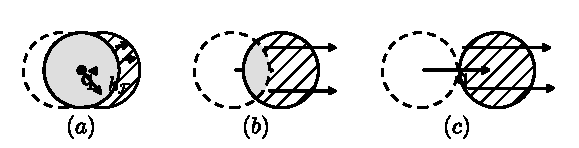
\includegraphics[width=0.72\textwidth]{fig_91.pdf}
\caption*{图 91\quad 对介电常数有贡献的费米球区域：(a) 小 $q$；(b) $q<2k_{F}$；(c) $q>2k_{F}$。}
\end{figure}

\begin{figure}[H]
\centering
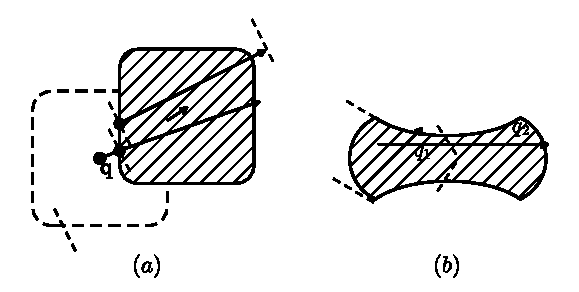
\includegraphics[width=0.72\textwidth]{fig_92.pdf}
\caption*{图 92\quad (a) 当 $\mathbf{q}$ 联接费米面上切线彼此平行的两点时出现 Kohn 异常；(b) 对给定的 $\mathbf{q}$ 方向，$q_{c}$ 可能有几个不同的值。}
\end{figure}

如果固定 $\mathbf{q}$ 的方向，我们预期 $q_{c}$ 出现在费米面在该方向上的极端卡钳口径（caliper dimension）处。如果我们能测出 $q_{c}$ 随方向的变化，就可以把费米面测绘出来——尽管（图 92(b)）对某一给定方向可能存在好几个 $q_{c}$ 值，对应于“直径”的极小值以及极大值。

这就是晶格谱中 \emph{Kohn 效应}（Kohn effect）的起源。波矢为 $q$ 的声子由于离子的运动而建立起具有 (5.16) 型分量的势。电子移动过来把这个场屏蔽掉。于是离子之间就通过这个被屏蔽的场相互作用，这个场将与 $\epsilon(\mathbf{q})$ 成反比。这样，离子之间的力将
%JOIN%
受到修正，而且这种振动模式的晶格频率将依赖于 $\epsilon(\mathbf{q})$（见 §6.11）。于是，$\epsilon$ 中的奇异性将反映在声子频率上。

在固体中传播的任何其他波动系统中，只要它们与传导电子有相互作用，也很可能观察到同样的效应，例如自旋波（§10.10）。原则上，这为研究费米面提供了一种普遍方法——尽管在实践中这一效应未必探测得到。

\section{Friedel 求和规则}

$\epsilon(\mathbf{q},0)$ 中的奇异性还有另一个有趣的后果。假设我们把式 (5.36) 代入点电荷屏蔽势的公式。按照式 (5.18) 与 (5.31)，应当得到

\begin{equation*}
\mathcal{U}(\mathbf{r}) = 4\pi e^2 \int \left\{ q^2 + \frac{4\pi e^2 n}{\frac{2}{3}\mathcal{E}_F} \left[ \frac{1}{2} + \frac{4k_F^2 - q^2}{8k_F q} \ln\left| \frac{2k_F + q}{2k_F - q} \right| \right] \right\}^{-1} e^{-i\mathbf{q}\cdot\mathbf{r}} \,\mathrm{d}\mathbf{q}
\tag{5.38}
\end{equation*}

此即距离 $r$ 处的势。不必真的完成这个计算，我们也很容易相信：$q = 2k_F$ 处的奇异性将作为一项特殊贡献显现在 $\mathcal{U}(\mathbf{r})$ 中；它将不再是光滑的指数函数，而会含有波数为 $2k_F$ 的振荡。

让我们不从式 (5.38) 出发来推导这一效应，而是循着 Friedel 提出的另一条颇为不同的论证路线。考虑一个球对称势 $\mathcal{U}(\mathbf{r})$。我们知道，在这种势存在时，Schrödinger 方程有一个形如下式的解

\begin{equation*}
\psi_{k,l} \sim \frac{1}{r} \sin\left( kr - \tfrac{1}{2}l\pi + \eta_l \right) P_l(\cos\theta)
\tag{5.39}
\end{equation*}

它在远处成立。式中 $P_l(\cos\theta)$ 是 $l$ 阶的普通球谐函数。我们现在考虑的不是散射问题，而是一个“自由”电子的定态；这个空间中除了位于中心的势 $\mathcal{U}(\mathbf{r})$ 之外空无一物。

像 (5.39) 这类解的存在——与 $\mathcal{U}(\mathbf{r}) = 0$ 时的对应解相比，其相位移动了一个量 $\eta_l$——正是求解这类势的散射问题的\emph{分波法}（partial wave method）的核心（参见 §3.9）。众所周知，像 (5.39) 这样的函数可与表示初态的平面波 $\exp(i\mathbf{k}\cdot\mathbf{r})$ 相匹配，而散射部分便可以计算出来。\emph{微分散射截面}由下式给出

\begin{equation*}
\sigma(\theta) = \frac{1}{k^2} \left| \sum_{l=0}^{\infty} (2l+1)\, e^{i\eta_l} \sin\eta_l \, P_l(\cos\theta) \right|^2 .
\tag{5.40}
\end{equation*}

但还是回到我们的定态 (5.39)。假设我们取它们作为体系的基本本征态，并像对待平面波态那样，按能量递增的次序把它们逐个填满。为了便于计数状态，方便的办法是换用另一类边界条件——明显的规则是在 $r = R$ 处 $\psi_k = 0$，就好像我们有一个半径为 $R$ 的大球，原子置于中心。于是 $k$ 的“允许”值必须满足

\begin{equation*}
kR - \tfrac{1}{2}l\pi + \eta_l = \text{integer} \times \pi .
\tag{5.41}
\end{equation*}

倘若我们的球是空的，使得所有相移（phase shift）$\eta_l$ 都为零，那么 $k$ 的“允许”值就应当是集合

\begin{equation*}
k_n = \frac{\left(n + \tfrac{1}{2}l\right)\pi}{R} .
\tag{5.42}
\end{equation*}

当然，对每一个 $n$ 值有许多不同的 $l$ 值，而对每个 $l$ 又有 $(2l+1)$ 个不同的波函数。但是可以证明——事实上，由关于本征值分布的一个普遍定理即可推出——能量小于 $\mathcal{E}_F$（即波矢小于 $k_F$）的态的总数，在这种方案下与 §1.6 中所用的更常见的立方盒情形相同。

\begin{figure}[H]
\centering
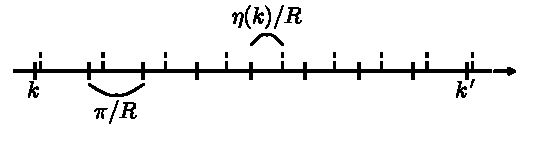
\includegraphics[width=0.72\textwidth]{fig_93.pdf}
\caption*{图 93\quad （译注：原书本图未附图注文字；图中沿 $k$ 轴标出"允许"值，相移使其移动一个量 $\eta(k)/R$，相邻间隔为 $\pi/R$。）}
\end{figure}

但原子位于中心时，各 $\eta_l$ 不为零，所以 $k$ 的“允许”值并不恰好落在 $k_n$ 处；它们将移动一个量 $\eta_l/R$。而 $\eta_l$ 又随 $k$ 变化。由图 93 容易看出，在 $k$ 轴上的两点 $k$ 与 $k'$ 之间，新的集合将含有

\begin{equation*}
\{\eta_l(k) - \eta_l(k')\}/\pi
\end{equation*}

个新的允许值。

现在假设（这是合理的）$\eta_l$ 在 $k = 0$ 处趋于零。把各个能级填充到同一费米波矢 $k = k_F$ 所需的新电子总数必为

\begin{equation*}
Z = \frac{2}{\pi} \sum_l (2l+1)\, \eta_l(k_F)
\tag{5.43}
\end{equation*}

这里对给定的 $l$ 计入了 $(2l+1)$ 个态，再加上电子的 2 个自旋态。我们已把这个数取作 $Z$，即杂质与溶剂金属之间的价电子数之差，因为恰好需要这么多的额外电子聚集在杂质附近来中和它的电荷。

这就是 \emph{Friedel 求和规则}（Friedel sum rule）。它依据两条普遍原理：杂质的电荷必须在有限距离内被过剩的电子所中和；在远离杂质处，费米波矢 $k_F$ 必须与纯净完整晶体中的相同。

这个公式为计算杂质的散射截面提供了一种极有用的方法。我们选取某个函数，例如带一个可调参数 $\lambda$ 的屏蔽 Coulomb 势 (5.29)。我们算出诸相移，并求出使它们满足 (5.43) 的 $\lambda$ 值。利用这些 $\eta_l$ 值，便可由分波公式 (5.40) 求得散射截面。这一步骤给出相当好的结果，而且对函数 $\mathcal{U}(\mathbf{r})$ 的形状不很敏感。原则上，它肯定比——比如说——在 Born 近似中使用 (5.38) 的矩阵元要好。传导电子太慢，那种做法并不成立。

但现在来考虑与像 (5.39) 那样带相移的波相联系的电子密度。在距原子很远的 $r$ 处，我们将发现多余电荷

\begin{align*}
\delta\rho &= e \sum_l (2l+1) \int_0^{k_F} \left\{ |\psi_{k,l}(\eta_l)|^2 - |\psi_{k,l}(0)|^2 \right\} \frac{2R}{\pi}\, \mathrm{d}k \\
&= \frac{e}{2\pi^2} \sum_l (2l+1) \int_0^{k_F} \left\{ \sin^2\left(kr - \tfrac{1}{2}l\pi + \eta_l\right) - \sin^2\left(kr - \tfrac{1}{2}l\pi\right) \right\} \frac{1}{r^2}\, \mathrm{d}k \\
&= \frac{e}{2\pi^2} \sum_l (2l+1) \int_0^{k_F} \sin\left(2kr - l\pi + \eta_l\right) \sin\eta_l \, \frac{1}{r^3}\, \mathrm{d}(kr) \\
&\sim \frac{e}{2\pi^2} \sum_l (2l+1) \left(-1\right)^l \sin\eta_l \, \frac{\cos(2k_F r + \eta_l)}{r^3}
\tag{5.44}
\end{align*}

这里对半径为 $R$ 的球中的波函数 (5.39) 使用了归一化因子 $(2\pi R)^{-\frac{1}{2}}$，并略去了在 $r$ 很大时更快趋于零的各项。

这就是与 (5.38) 中的奇异性相联系的振荡电荷密度。它仅以 $1/r^3$ 的方式趋于零，因此绝非可忽略的效应。有趣的是，杂质附近的电荷并不是简单地堆积起来；存在 $\delta\rho$ 为负的区域，在那里电子实际上被驱赶出去。这一点在与杂质间相互作用以及合金中 Knight 位移（Knight shift）有关的现象中具有重要意义（见 §10.2）。

实际情况是：这份局域电荷并不是束缚在杂质周围的一两个电子的电荷。它来自费米气体中的快电子被吸引向杂质——它们倾向于在邻近处稍作逗留，并在那里挤得更紧。电子波长的陡峭截断于是引起干涉效应，在散射中心四周投下电荷的晕环。

\begin{figure}[H]
\centering
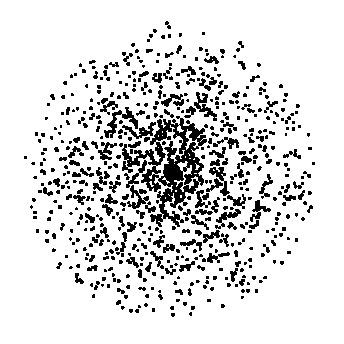
\includegraphics[width=0.72\textwidth]{fig_94.pdf}
\caption*{图 94\quad 杂质周围的电荷晕}
\end{figure}

当\emph{过渡金属}溶入“正常”金属时，我们必须考虑未满的 d 壳层。正如 §3.10 中所见，自由原子的 d 轨道表现为一个\emph{共振}；在其中，如式 (3.81) 那样，\emph{d 相移}在宽度为 $W$ 的能量区间内迅速通过 $\pi/2$。由 Friedel 求和规则 (5.43) 可知，当我们穿越共振时，最多可达 10 个电子的电荷迅速在杂质上积累起来。但杂质上的总电荷必须自行稳定以求中和它的核电荷；离子中“d 电子”的数目必须与自由原子中的大致相同。这意味着溶剂金属的费米能级必须位于共振区之内。

自由原子 d 壳层中的电子总是磁极化的：按照 Hund 规则，它们的自旋排列成与 Pauli 原理相容的最大磁矩。例如在 Mn 中，全部 5 个 d 电子可以取相同的自旋。当原子溶入另一金属时，这种倾向可能延续下来，尽管自旋极化已不能再归因于一个定态原子能级。

例如，假设杂质恰好拥有过剩的“向上”自旋电子。对于另一个自旋相同的电子来说，遇到这个原子时，它看到的是一个位于费米能级之下的共振，并被吸引进去（图 95）。于是“向上”自旋密度得到增强，极化态得以稳定。反之，对“向下”自旋的电子，d--d 交换相互作用把共振的能量推高，从而耗减杂质内向下自旋的密度。净效果必须补偿离子的总电荷；但在合适的溶剂中，我们还可能观察到一种动力学的多电子磁矩，其方向缓慢涨落，而大小与自由原子的磁矩相当。这一过程解释了过渡金属稀合金的许多特殊的电学和磁学性质（见 §10.6）。

\begin{figure}[H]
\centering
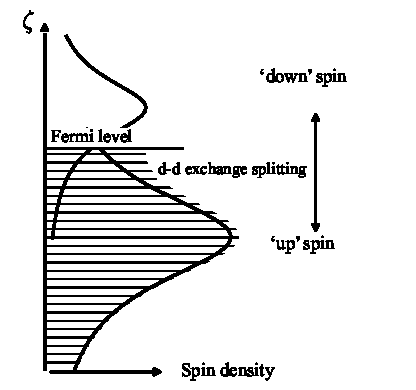
\includegraphics[width=0.72\textwidth]{fig_95.pdf}
\caption*{图 95\quad 磁性杂质处电子的共振，杂质极化沿"向上"方向}
\end{figure}

\section{半导体的介电常数}

金属的宏观介电常数当 $\mathbf{q} \to 0$ 时趋于无穷，因为金属具有高电导率。这个结果由 (5.16) 和 (5.21) 得出。然而在半导体或绝缘体中，电导率很小；除载流子的热激发之外，它可取为零。静态介电常数 $\epsilon(\mathbf{q},0)$ 在长波下应保持有限。

这源于已满态与空态之间的能隙。形如 (5.16) 的求和中的分母在 $\mathbf{q} = \mathbf{0}$ 处并不为零，而是保持有限。

要计算一个实际半导体的 $\epsilon(\mathbf{q},0)$，需要能带结构的细致模型。我们不能使用 §5.1 的简单理论，因为未微扰的电子态 $|\mathbf{k}\rangle$ 已不再是简单的平面波。不过很容易证明：只需把微扰波 $\exp(i\mathbf{q}\cdot\mathbf{r})$ 的矩阵元的平方引入求和 (5.16)，便得到正确的公式

\begin{equation*}
\epsilon(\mathbf{q},\omega) = 1 + \frac{4\pi e^2}{q^2} \sum_{\mathbf{k},\mathbf{g}} \frac{\left| \langle \mathbf{k}|\, e^{i\mathbf{q}\cdot\mathbf{r}}\, |\mathbf{k}+\mathbf{q}+\mathbf{g}\rangle \right|^2 \left\{ f^0(\mathbf{k}) - f^0(\mathbf{k}+\mathbf{q}+\mathbf{g}) \right\}}{\mathcal{E}(\mathbf{k}+\mathbf{q}+\mathbf{g}) - \mathcal{E}(\mathbf{k}) - \hbar\omega + i\hbar\alpha} .
\tag{5.45}
\end{equation*}

我们必须计入倒格矢 $\mathbf{g} \neq \mathbf{0}$ 的那些项，因为 Bloch 函数之间 $\exp(i\mathbf{q}\cdot\mathbf{r})$ 的矩阵元在二者的波矢相差 $\mathbf{q}+\mathbf{g}$ 时并不为零。这里的情形与 §2.7 的衍射理论本质上相同。

我们不打算精确求值 (5.45)，但可以按下面的办法得到一个粗略近似。让我们采用简约区图式。于是，当 $|\mathbf{k}\rangle$ 是一个已满态时，可用的空态全都在下一个带中；若 $\mathbf{q}$ 很小，$|\mathbf{k}+\mathbf{q}+\mathbf{g}\rangle$ 这时指的是一个几乎竖直地处在 $|\mathbf{k}\rangle$ “正上方”的态。假定能量分母对所有的 $\mathbf{k}$ 值都相同：我们把它取为带隙宽度

\begin{equation*}
\mathcal{E}(\mathbf{k}+\mathbf{q}+\mathbf{g}) - \mathcal{E}(\mathbf{k}) \approx \mathcal{E}_{\mathrm{gap}} .
\tag{5.46}
\end{equation*}

现在我们要对每个 $\mathbf{k}$ 值计算

\begin{equation*}
\sum_{\mathbf{g}} \left| \langle \mathbf{k}|\, e^{i\mathbf{q}\cdot\mathbf{r}}\, |\mathbf{k}+\mathbf{q}+\mathbf{g}\rangle \right|^2
\tag{5.47}
\end{equation*}

为此可以利用下面的定理：——

\begin{equation*}
\sum_n \left( \mathcal{E}_n - \mathcal{E}_s \right) \left| \langle n|\, e^{i\mathbf{q}\cdot\mathbf{r}}\, |s\rangle \right|^2 = \frac{\hbar^2 q^2}{2m},
\tag{5.48}
\end{equation*}

它对 哈密顿量 $\mathcal{H}$ 的本征态 $|n\rangle$ 与 $|s\rangle$ 之间 $\exp(i\mathbf{q}\cdot\mathbf{r})$ 的矩阵元成立，此 哈密顿量的动能项为 $-(\hbar^2/2m)\nabla^2$。这个定理的证明（它是众所周知的\emph{振子强度求和规则}（sum rule for oscillator strengths）的推广）来自把双对易子

\begin{equation*}
\left[ \left[ \mathcal{H},\, e^{i\mathbf{q}\cdot\mathbf{r}} \right],\, e^{-i\mathbf{q}\cdot\mathbf{r}} \right]
\tag{5.49}
\end{equation*}

的期望值在态 $|s\rangle$ 中展开。

如果我们取 $|s\rangle$ 实际上就是我们的态 $|\mathbf{k}\rangle$，并且像 (5.46) 那样，假设对求和中唯一重要的那些态 $|n\rangle$ 有

\begin{equation*}
\mathcal{E}_n - \mathcal{E}_s = \mathcal{E}(\mathbf{k}+\mathbf{q}+\mathbf{g}) - \mathcal{E}(\mathbf{k}) \approx \mathcal{E}_{\mathrm{gap}}
\tag{5.50}
\end{equation*}

那么我们就得到

\begin{equation*}
\sum_{\mathbf{g}} \left| \langle \mathbf{k}|\, e^{i\mathbf{q}\cdot\mathbf{r}}\, |\mathbf{k}+\mathbf{q}+\mathbf{g}\rangle \right|^2 \approx \frac{1}{\mathcal{E}_{\mathrm{gap}}} \, \frac{\hbar^2 q^2}{2m} .
\tag{5.51}
\end{equation*}

把 (5.46) 和 (5.51) 代入 (5.45)，并把满带中 $n$ 个电子各自的贡献加起来（同时也计入 $|\mathbf{k}\rangle$ 为空而 $|\mathbf{k}+\mathbf{q}+\mathbf{g}\rangle$ 为满的那些项），便得

\begin{align*}
\epsilon(\mathbf{q},0) &\approx 1 + \frac{4\pi e^2}{q^2}\, \frac{n}{\mathcal{E}_{\mathrm{gap}}}\, \frac{\hbar^2 q^2}{2m}\, \frac{2}{\mathcal{E}_{\mathrm{gap}}} \\
&= 1 + \frac{4\pi n e^2 \hbar^2}{m\left(\mathcal{E}_{\mathrm{gap}}\right)^2} \\
&= 1 + \left( \frac{\hbar\omega_p}{\mathcal{E}_{\mathrm{gap}}} \right)^2 ,
\tag{5.52}
\end{align*}

其中我们定义了\emph{等离体频率}（plasma frequency）

\begin{equation*}
\omega_p = \left( \frac{4\pi n e^2}{m} \right)^{\frac{1}{2}}
\tag{5.53}
\end{equation*}

——这个参量的物理意义稍后即将显现。

公式 (5.52) 表明，静态介电常数在 $\mathbf{q} = \mathbf{0}$ 处趋于一个常数。这应当就是固体观测到的宏观介电常数。能隙越小，介质越容易极化，即 $\epsilon$ 值越大。当然，我们不能把所取的 $\mathcal{E}_{\mathrm{gap}}$ 值等同于导带底与价带顶之间的光学间隙；它更像是简约区中竖直方向上相互对着的那些态之间的平均能量距离。

于是，半导体中杂质周围的静电场并不像金属中那样受到屏蔽：它只是简单地缩减为 $e^2/\epsilon r$，其中 $\epsilon$ 是静态介电常数。这使得束缚电子态得以在杂质周围形成——这就是\emph{杂质能级}（impurity levels），我们将在 §6.4 中再次讨论。当然，如果介质中存在残余载流子密度 $n_0$，那么在远处我们仍会看到杂质受到经典屏蔽，正如 Debye--Hückel 公式 (5.26)、(5.29) 所给出的那样。

\section{等离体振荡}

现在我们考虑时间相关的效应，其中“外”微扰场的频率 $\omega$ 不为零。这里会出现几个重要现象。最明显的一个是：(5.16) 或 (5.45) 中的 $\hbar\omega$ 恰好与被微扰所混合的一对态之间的能量差相合，也就是说，对占据能级中的某个 $\mathbf{k}$ 值，

\begin{equation*}
\mathcal{E}(\mathbf{k}+\mathbf{q}+\mathbf{g}) - \mathcal{E}(\mathbf{k}) = \hbar\omega .
\tag{5.54}
\end{equation*}

这时 $\epsilon(\mathbf{q},\omega)$ 中出现奇异性——或者说虚部 $i\hbar\alpha$ 变为占优。这恰恰对应于电子的光学吸收（或发射），即电子从态 $|\mathbf{k}\rangle$ 跃迁到态 $|\mathbf{k}+\mathbf{q}+\mathbf{g}\rangle$。我们把这称为体系的一种\emph{单粒子激发}（single-particle excitation）。这些效应我们在 §8.5 中再来讨论。

但假设 $\hbar\omega$ 很大——远大于 (5.16) 分母中的任何一个能量差。我们可以把求和改写成如下形式：

\begin{equation*}
\epsilon(\mathbf{q},\omega) = 1 + \frac{4\pi e^2}{q^2} \sum_{\mathbf{k}} \frac{2f^0(\mathbf{k}) \left\{ \mathcal{E}(\mathbf{k}) - \mathcal{E}(\mathbf{k}+\mathbf{q}) \right\}}{(\hbar\omega)^2 - \left\{ \mathcal{E}(\mathbf{k}) - \mathcal{E}(\mathbf{k}+\mathbf{q}) \right\}^2} .
\tag{5.55}
\end{equation*}

于是可以把分母就取为 $(\hbar\omega)^2$，并把分子按 $\mathbf{q}$ 的幂展开。头几项为零，我们便得到

\begin{align*}
\epsilon(\mathbf{q},\omega) &= 1 + \frac{4\pi e^2}{q^2} \sum_{\mathbf{k}} \frac{f^0(\mathbf{k})}{(\hbar\omega)^2} \left( -q^2 \frac{\partial^2 \mathcal{E}}{\partial k^2} \right) \\
&= 1 - \frac{4\pi n e^2 \hbar^2}{\hbar^2 \omega^2 m} \\
&= 1 - \frac{\omega_p^2}{\omega^2} ,
\tag{5.56}
\end{align*}

其中 $\omega_p$ 是由 (5.53) 定义的等离体频率。

这是对自由电子导出的。但同样的结果也可以由 (5.45) 得到，后者可以改写成

\begin{equation*}
\epsilon(\mathbf{q},\omega) = 1 + \frac{4\pi e^2}{q^2} \sum_{\mathbf{k},\mathbf{g}} \frac{2f^0(\mathbf{k}) \left| \langle \mathbf{k}|\, e^{i\mathbf{q}\cdot\mathbf{r}}\, |\mathbf{k}+\mathbf{q}+\mathbf{g}\rangle \right|^2 \left\{ \mathcal{E}(\mathbf{k}) - \mathcal{E}(\mathbf{k}+\mathbf{q}+\mathbf{g}) \right\}}{(\hbar\omega)^2 - \left\{ \mathcal{E}(\mathbf{k}) - \mathcal{E}(\mathbf{k}+\mathbf{q}+\mathbf{g}) \right\}^2} .
\tag{5.57}
\end{equation*}

如果分母可以当作常数处理，即如果

\begin{equation*}
\hbar\omega \gg \mathcal{E}(\mathbf{k}) - \mathcal{E}(\mathbf{k}+\mathbf{q}+\mathbf{g})
\tag{5.58}
\end{equation*}

对所有被占据的 $\mathbf{k}$，以及对所有矩阵元不可忽略的 $\mathbf{g}$ 都成立，那么我们可以把求和规则 (5.48) 用于对 $\mathbf{g}$ 的求和，对被占据态中 $n$ 个电子的每一个都得到一项 $(4\pi e^2/m\omega^2)$。

公式 (5.56) 表明，当 $\omega \to \omega_p$ 时 $\epsilon \to 0$。而当 $\epsilon = 0$ 时，由 (5.15)，我们有

\begin{equation*}
\mathcal{U} = \frac{\mathcal{V}}{\epsilon} \to \infty .
\tag{5.59}
\end{equation*}

换言之，一个无穷小的“外场” $\mathcal{V}$ 会引起很大的有效场 $\mathcal{U}$：体系是自激发的。频率 $\omega_p$ 是电子气的一个固有振荡模式——称为\emph{等离体模式}（plasma mode）。

这个结果可以用一个初等的论证导出。设体积密度为 $n$ 的电子相对于晶格的固定正电荷背景整体移动一段距离 $\mathbf{x}$。这就建立起一个极化

\begin{equation*}
\mathbf{P} = ne\mathbf{x},
\tag{5.60}
\end{equation*}

它转而又产生一个电场

\begin{equation*}
\mathbf{E} = -4\pi\mathbf{P} .
\tag{5.61}
\end{equation*}

于是每个电荷的运动方程为

\begin{equation*}
m\ddot{\mathbf{x}} = e\mathbf{E} = -4\pi n e^2 \mathbf{x},
\tag{5.62}
\end{equation*}

它定义了频率为 $\omega_p$ 的简谐振荡。

等离体频率对应于相当大的能量，约为 10–20 eV，所以这些模式不会在热能量下被激发。但如果让电子穿过金属薄膜，就可以观察到相应于这些模式中一个或多个量子被激发的能量损失。有趣的是，即使在半导体中，$\omega_p$ 也只依赖于价带中的总电子密度。这是因为只要等离体能量比价带与导带之间的能量差高出相当多——通常后者在 5 eV 以下——条件 (5.58) 就会成立。另一方面，离子芯中的电子不作贡献；它们束缚得太紧。这些能级与导带中的态之间的能量差远大于 $\hbar\omega_p$。

我们可以把 $\epsilon(\mathbf{q},\omega)$ 展开到 $\mathbf{q}$ 的更高次幂，求出使 $\epsilon$ 为零的 $\omega$ 作为 $\mathbf{q}$ 的函数。对自由电子，结果是

\begin{equation*}
\omega(q) = \omega_p \left[ 1 + \frac{3}{10}\, \frac{q^2 v_F^2}{\omega_p^2} + \ldots \right],
\tag{5.63}
\end{equation*}

其中 $v_F$ 是费米面上电子的速度。这样，等离体振荡可以在各种波长下发生——这些模式中的量子可称为\emph{等离激元}（plasmon）。但色散定律 (5.63) 表明，频率对 $q$ 的依赖并不强；等离激元倾向于成为只在介质中缓慢移动的局域化振荡。

严格说来，$\epsilon(\mathbf{q},\omega)$ 是复数：(5.55) 和 (5.57) 表示的是它的实部（假定 $\alpha$ 很小）。虚部由下式给出

\begin{equation*}
\epsilon_2(\mathbf{q},\omega) = \frac{-4\pi^2 e^2}{q^2} \sum_{\mathbf{k}} \left\{ f^0(\mathbf{k}) - f^0(\mathbf{k}+\mathbf{q}) \right\} \delta\!\left\{ \mathcal{E}(\mathbf{k}+\mathbf{q}) - \mathcal{E}(\mathbf{k}) - \hbar\omega \right\},
\tag{5.64}
\end{equation*}

其中的 $\delta$ 函数来自积分 (5.16) 中位于实轴附近的极点

\begin{equation*}
\hbar\omega = \mathcal{E}(\mathbf{k}+\mathbf{q}) - \mathcal{E}(\mathbf{k})
\tag{5.65}
\end{equation*}

处。关于这个公式，有趣的一点是：当

\begin{equation*}
\omega \geqslant q v_F,
\tag{5.66}
\end{equation*}

时它为零；也就是说，此时 $\omega$ 大到仅凭波矢改变 $\mathbf{q}$ 已不能把单个粒子从费米分布中激发出来。这表明等离体模式在这个频率之上不会迅速耗散。

由 (5.56) 还可导出与等离体振荡相联系的另一个有趣现象。如果它表示金属实际的介电常数——如同用长波长的高频电
场所测得的那样——我们可以写出介质的一个\emph{复折射率}（complex refractive index）$\mathbf{N}$：
\begin{equation*}
\mathbf{N}^{2}=\epsilon(\mathbf{q},\omega)\approx 1-\frac{\omega_{p}^{2}}{\omega^{2}}. \tag{5.67}
\end{equation*}
若 $\omega<\omega_{p}$，则 $\epsilon$ 为负，$\mathbf{N}$ 为纯虚数，这引起光的\emph{全反射}。但若 $\omega>\omega_{p}$，则 $\epsilon$ 为正，$\mathbf{N}$ 为实数；当沿垂直于表面的方向观察时，金属就变成\emph{透明}的。当对电子引入散射机制之后，这个理论要稍作修改（见 §8.6），但在碱金属中确实观察到了\emph{紫外透明}现象。

\section{准粒子与内聚能}

当然，上述基于介电常数的分析只是一种近似。实质性的步骤在 §5.1 中已经完成：在那里假定势的每一个 Fourier 分量都可以独立地处理。这在使用术语上称为\emph{无规相位近似}（Random Phase Approximation），在对这个问题几乎所有更细致的分析中都不得不采用这一假定。

除了作一些一般性的评论之外，我们将不讨论这些更复杂的理论。结果发现，与 Coulomb 势相联系的电子之间的强长程相互作用，可以约化成类似式 (5.29) 的屏蔽相互作用。电子不仅在杂质周围形成电荷云、把远距离处的场屏蔽掉；每个电子还可以说都随身携带着自己的电荷云——实际上是一个“正”的云，对应于把“其他”电子有效地排除在它的邻域之外。

反过来，在晶体中到处运动的\emph{正电子}（positron）会把一个“负”的电荷云吸引到自己周围。因此，金属中\emph{正电子湮灭}（positron annihilation）的速率，由于正电子中心处电子概率密度的增强，要比未受扰动的均匀电子气情形略高一些。但是，多体效应并不会严重干扰对湮灭过程中所发射的两个 $\gamma$ 射线量子方向之间角关联的简单解释。由于认为正电子在湮灭之前已在晶格中静止下来，发射方向对相反方向的任何偏离，必定来自湮灭电子所提供的动量（图 96）。因此，角 $\theta$ 的分布给出了传导电子气中动量分布的一种量度，这或许会被证明是对金属与合金电子结构理论的一种有用检验。

\begin{figure}[H]
\centering
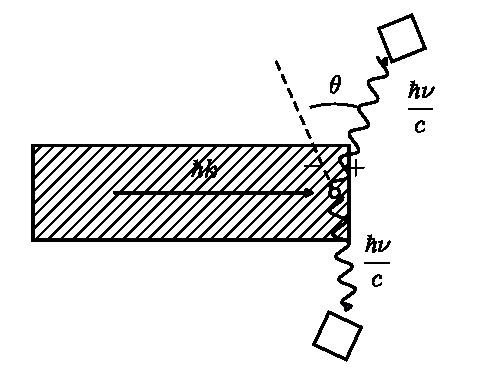
\includegraphics[width=0.72\textwidth]{fig_96.pdf}
\caption*{图 96\quad 正电子湮灭中的动量守恒}
\end{figure}

严格说来，一个带着正电荷晕的电子，需要用非常复杂的波函数才能得到对它的恰当描述。然而，它的行为确实非常像一个粒子，因为它携带着电子电荷 $e$。“其他”电子的效应，是改变这个量子态的能量与波矢之间的关系；例如，可以有
\begin{equation*}
\mathcal{E}(\mathbf{k})=\frac{\hbar^{2}k^{2}}{2m^{*}}, \tag{5.68}
\end{equation*}
其中 $m^{*}$ 并不完全等于普通的自由电子质量 $m$。结果发现，这些准粒子（quasi-particle）在费米能级附近是相当稳定的，但在远离费米面时便趋于瓦解和耗散。这一点对于输运理论以及费米面概念的形式论证十分重要。

准粒子图像实际上正是电子气的\emph{元激发}（elementary excitations）谱的一种表示。虽然我们不能对真实金属精确地算出这个谱，但对于处在正凝胶（§5.1）中的、具有相应密度的理想电子气，我们可以对它的性质作出相当好的估计。例如，这个模型的基态能量就告诉我们一些关于金属内聚能（cohesive energy）（§4.3）的信息。Wigner 和 Seitz 的粗糙假定——电子把它到访的原胞中的所有其他传导电子统统驱赶出去——可以换成对电子与其屏蔽云之间静电相互作用的直接计算，从而对金属键合中电子关联（electron correlation）的效应作出好得多的估计。

同样，我们应当预期两个准粒子之间的相互作用相当弱，多少就如同通过屏蔽的 Coulomb 相互作用那样。因此，我们的系统符合\emph{Fermi 液体}（Fermi liquid）的 Landau 模型：其中较低的诸能级用把一个或多个准粒子激发到更高的态来表示，就好像我们拥有一团极低温度下的由\emph{独立}费米子（fermions）组成的气体一样。但是，当我们把越来越多的粒子激发到费米能级之上时，就必须计及它们之间的相互作用。这些相互作用由下列形式的附加能量项表示：
\begin{equation*}
E_{2}=\frac{1}{2}\sum_{\mathbf{k},\sigma;\,\mathbf{k}',\sigma'}f(\mathbf{k},\sigma;\,\mathbf{k}',\sigma')\,\delta n(\mathbf{k},\sigma)\,\delta n(\mathbf{k}',\sigma') \tag{5.69}
\end{equation*}
其中 $\delta n(\mathbf{k},\sigma)$ 是当我们从基态过渡到系统的某个较高能级时，波矢为 $\mathbf{k}$、自旋为 $\sigma$ 的准粒子模式的占据数的变化。

Landau 模型的参数决定了传导电子气的谱，从而决定了诸如电子比热（§4.7）这样的一些性质。相互作用项 $f(\mathbf{k},\sigma;\mathbf{k}',\sigma')$ 的一个重要特点是：它确实依赖于两个电子的自旋的相对取向。在普通金属密度下，这种\emph{交换}（exchange）力有利于平行排列——这本质上是因为 Pauli 原理使两个自旋相同的电子不致占据空间同一点，从而增强了关联效应并稍稍降低了它们的相互静电势能。这个效应并不大，但显然在金属磁性的理论中起着重要作用（见 §§10.2--10.5）。

\section{Mott 转变}

还有一种本质上起因于电子之间作用力的定性效应，它并不常被观察到，但在原理上颇为重要。设想我们把大量的氢原子（或 Na 原子——或者任何每个原胞含有奇数个电子的原子阵列）缓慢地聚拢在一起。按照 §4.1 中阐述的原理，每个原子上的电子波函数将发生交叠，能带将会形成，固体就应当立即变成导体。而且看起来，无论原子相距多远，这都应当发生。

这是一个悖论性的结果，难以令人相信。实际上，很可能并非如此。§3.4 中曾提示，一组局域轨道（localized orbitals）$\phi_{a}(\mathbf{r}-\mathbf{l})$ 与一组 Bloch 函数 $\phi_{\mathbf{k}}(\mathbf{r})$ 形式上等价；但这种等价性只有在我们忽略 Pauli 原理和电子间相互作用时才成立。如果每个原子有两个电子，那么满带中所有态 $\phi_{\mathbf{k}}(\mathbf{r})$ 构成的行列式波函数，与所有局域原子轨道\footnote{严格说来，这里我们应当指的是 Wannier 函数（见 §6.2）。但是，假如我们假定当原子相距很远时紧束缚近似成立，论证也完全一样。}$\phi_{a}(\mathbf{r}-\mathbf{l})$ 构成的行列式相同。但如果每个原子只有一个电子，半满带中诸态的行列式就不等同于局域轨道的行列式。它倾向于把两个电子安放到某些原子上，而让另一些原子近乎空着——这样的电荷分布可能给系统的总 Coulomb 能贡献一些很大的正项。因此，作为系统的试探波函数，局域态的集合也许比离域（delocalized）的能带态集合更好。前一类波函数描述绝缘体，后一类描述导体。

为了区分这两者，我们可以采用如下的论证。设想从局域态阵列中取出一个电子。它将在身后留下一个空的离子，即一个正电荷。电子会被这个离子吸引，甚至可能在它那里形成一个束缚态，以致它实际上并不能自由地穿越晶体去传导电流。但假如已经有许多这样的电子存在，它们就会屏蔽离子的电荷，此时离子的势可以取为如下形式：
\begin{equation*}
-\frac{e^{2}}{r}\,e^{-\lambda r}, \tag{5.70}
\end{equation*}
如同式 (5.29) 一样。若已电离电子的密度为 $n$，则按照式 (5.22)，
\begin{equation*}
\lambda^{2}\approx\frac{4me^{2}n^{1/3}}{\hbar^{2}} \tag{5.71}
\end{equation*}
（利用了式 (3.3)、(3.4) 和 (4.3)）。

普通的 Coulomb 场是能够束缚一个电子的。最低的态——氢原子的基态——具有半径
\begin{equation*}
a_{H}=\frac{\hbar^{2}}{me^{2}}. \tag{5.72}
\end{equation*}
如果屏蔽半径 $1/\lambda$ 小于 $a_{H}$，那么连这个态也无法被束缚。因此，具有势 (5.70) 的电离原子能够重新俘获从它那里取走的电子，其条件是
\begin{gather*}
\lambda<a_{H}^{-1}, \\
\text{即}\quad n^{-1/3}>4a_{H}. \tag{5.73}
\end{gather*}
如果我们原子的平均间距大于 4 个原子单位，金属态就不能自我维持，系统应当变成绝缘体。而且，这是一种合作效应；每一个额外的自由电子都有助于使其余的电子松脱。即使我们没有把式 (5.73) 中的数字 4 算对，这个转变在原则上看来也会相当陡峭；把我们的氢或 Na 原子聚拢起来，我们应当会看到它们在某个确定的原子间距处突然从绝缘体转变为金属。

\emph{Mott 转变}（Mott transition）已经在某些过渡金属氧化物中观察到，它们在某个温度以上非常突然地变成导电的。这个理论也可以应用于半导体中的杂质中心，此时须对 $a_{H}$ 加以修正，即乘以半导体的体介电常数（如 §5.6 中那样；原书误印作 §5.5）（见 §6.4）。

上述论证其实与 \emph{Wigner 假说}密切相关：密度极低的电子气将倾向于“结晶”。令 $r_{0}$ 为一个电子所占据的球的平均半径，即
\begin{equation*}
\tfrac{4}{3}\pi r_{0}^{3}=1/n. \tag{5.74}
\end{equation*}
每个电子的势能，由于在它周围有一圈带正电的背景凝胶球，将是
\begin{equation*}
-e^{2}/2r_{0}. \tag{5.75}
\end{equation*}
的量级。但每个电子由于被限制在这个球的区域之内，还会有量级为
\begin{equation*}
\hbar^{2}/mr_{0}^{2} \tag{5.76}
\end{equation*}
的零点能（zero-point energy）。因此，当
\begin{gather*}
e^{2}/2r_{0}\geqslant\hbar^{2}/mr_{0}^{2}, \\
\text{即}\quad r_{0}\geqslant 2a_{H}. \tag{5.77}
\end{gather*}
时，势能将占上风。其中的数值因子，如同式 (5.73) 中的一样，不必当真；而且在什么样的条件下这个转变实际上可能被观察到，也完全不清楚。尽管如此，认识到第 4 章的简单能带理论以及本章的简单电子关联理论的这些局限性，是十分重要的。

 % 本文件由 scripts/assemble.py 自动装配，勿手改（改 parts/ 后重跑）
% 第6章 电子动力学

% 第6章 Dynamics of Electrons

\chapter{电子动力学}

\epigraphbook{自由是对必然性的认识。}{ENGELS}

\section{普遍原理}

到目前为止，我们讨论的都是固体的静态性质。但是许多最重要的物理现象，例如电导率和热导率，都是动力学效应——是外力和外场作用的结果。我们需要一套关于这类现象的理论，尤其是把它应用于传导电子（conduction electrons）的理论。

初等的原理非常简单。我们先要计算处于态 $|\mathbf{k}\rangle$ 的电子的\emph{速度}。这个态具有能量 $\mathcal{E}(\mathbf{k})$；在初等波力学中，我们给它配上一个随时间变化的因子，仿佛它具有频率

\begin{equation*}
\nu_{\mathbf{k}} = \frac{1}{\hbar}\,\mathcal{E}(\mathbf{k}).
\tag{6.1}
\end{equation*}

但在波动理论中，如果我们假定介质是色散性的，那么频率在此附近的波包，其\emph{群速}（group velocity）应为

\begin{equation*}
\mathbf{v}_{\mathbf{k}} = \nabla_{\mathbf{k}}\,\nu_{\mathbf{k}} = \frac{1}{\hbar}\,\frac{\partial\mathcal{E}(\mathbf{k})}{\partial\mathbf{k}}.
\tag{6.2}
\end{equation*}

\emph{“处于态 $|\mathbf{k}\rangle$ 中”的电子，其速度正是 $\mathcal{E}(\mathbf{k})$ 在 k 空间中的梯度。}

对自由电子，这套做法完全有效：

\begin{equation*}
\mathcal{E}(\mathbf{k}) = \frac{\hbar^2 k^2}{2m},
\tag{6.3}
\end{equation*}

即

\begin{equation*}
\mathbf{v}_{\mathbf{k}} = \frac{\hbar\mathbf{k}}{m} = \frac{\mathbf{p}}{m},
\tag{6.4}
\end{equation*}

其中 $\mathbf{p}$ 是动量。从初等波力学大家都知道，这正是把电子看作一个在空间中自由运动的波包时它所具有的速度。

再者，量 $\hbar\mathbf{k}$ 在衍射现象（§2.8）中的表现也非常像一个\emph{动量}。很自然可以假定，加速的动力学定律具有如下形式

\begin{equation*}
\hbar\dot{\mathbf{k}} = \mathbf{F},
\tag{6.5}
\end{equation*}

其中 $\mathbf{F}$ 是作用在电子上的力。我们得到一条牛顿式的定律；\emph{晶体动量（crystal momentum）的变化率等于力。}

式 (6.2) 和式 (6.5) 这两条原理确实成立，但需要加以论证。我们必须说明，晶体晶格的存在究竟是如何深刻地改变电子的传播性质的；并且对表述这些简单定律时所涉及的近似，也要有些了解。证明相当繁复，需要分几步论证。

\section{Wannier 函数}

回忆一下我们在 §3.4 中用原子轨道 $\phi_n$ 给出的 Bloch 函数定义：

\begin{equation*}
\psi_{\mathbf{k},n} = \frac{1}{\sqrt{N}}\sum_{\boldsymbol{l}} e^{i\mathbf{k}\cdot\boldsymbol{l}}\,\phi_n(\mathbf{r}-\boldsymbol{l}).
\tag{6.6}
\end{equation*}

这是个相当漂亮的公式，因为它展示了一个波 $\exp(i\mathbf{k}\cdot\boldsymbol{l})$ 叠加在一组组局域的原子轨道上，给出每个格点处的相位和振幅。

\begin{figure}[H]
\centering
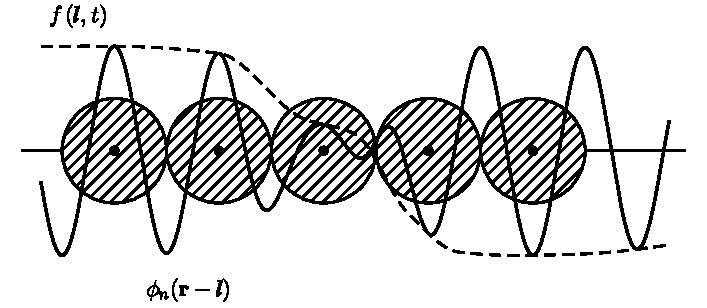
\includegraphics[width=0.72\textwidth]{fig_97.pdf}
\caption*{图 97\quad 叠加在原子轨道上的波。}
\end{figure}

为了表示动力学效应，我们可以试着按同一模式构造一个随时间变化的波函数

\begin{equation*}
\psi(\mathbf{r},t) \sim \sum_{\boldsymbol{l}} f(\boldsymbol{l},t)\,\phi_n(\mathbf{r}-\boldsymbol{l}),
\tag{6.7}
\end{equation*}

其中 $f(\boldsymbol{l},t)$ 将是一个包络函数（envelope function），表示叠加在局域原子轨道 $\phi_n(\mathbf{r}-\boldsymbol{l})$ 上的波在 $\boldsymbol{l}$ 附近处的强度。

但是紧束缚表述本身并不完全可行，原因在于正交化上的困难。事实上，式 (6.6) 所定义的函数并不是晶体势的 Schrödinger 方程的解。我们知道，需要取原子轨道的线性组合，例如

\begin{equation*}
\psi_{\mathbf{k}} = \frac{1}{\sqrt{N}}\sum_{\boldsymbol{l},m} e^{i\mathbf{k}\cdot\boldsymbol{l}}\,c_m\,\phi_m(\mathbf{r}-\boldsymbol{l}),
\tag{6.8}
\end{equation*}

其系数有待确定，以满足 Schrödinger 方程。因此，若不先解出 L.C.A.O.（原子轨道线性组合）问题——一件极其繁琐的准备工作——我们就无法使用 (6.7) 这种表示。

不过，我们仍然可以\emph{定义}出一些函数，使之具备我们本来希望局域原子轨道具有的那些性质。\emph{设存在一个函数 $a_n(\mathbf{r})$，使得第 $n$ 个能带中真正的 Bloch 函数由下式给出}

\begin{equation*}
\psi_{\mathbf{k},n} = \frac{1}{\sqrt{N}}\sum_{\boldsymbol{l}} e^{i\mathbf{k}\cdot\boldsymbol{l}}\,a_n(\mathbf{r}-\boldsymbol{l}).
\tag{6.9}
\end{equation*}

我们把这个新函数 $a_n$ 称为 \emph{Wannier 函数}（Wannier function）。它是位置的函数，但在一个布里渊区内与 $\mathbf{k}$ 无关。每一个电子能带都有一个不同的 Wannier 函数，正如紧束缚表述中每个原子轨道产生一个不同的能带一样。

式 (6.9) 很容易反演。如果我们已经用某种方法——例如 O.P.W.（正交化平面波）方法——解出了 Bloch 函数 $\psi_{\mathbf{k},n}$，那么就可以用一个合适的波因子去乘 (6.9)，并对一个区内所有 $\mathbf{k}$ 值求和：

\begin{align*}
\sum_{\mathbf{k}} e^{-i\mathbf{k}\cdot\boldsymbol{l}'}\,\psi_{\mathbf{k},n}(\mathbf{r}) &= \frac{1}{\sqrt{N}}\sum_{\mathbf{k},\boldsymbol{l}} e^{i\mathbf{k}\cdot(\boldsymbol{l}-\boldsymbol{l}')}\,a_n(\mathbf{r}-\boldsymbol{l}) \\
&= \sqrt{N}\sum_{\boldsymbol{l}} \delta_{ll'}\,a_n(\mathbf{r}-\boldsymbol{l}) \\
&= \sqrt{N}\,.\,a_n(\mathbf{r}-\boldsymbol{l}'). \tag{6.10}
\end{align*}

这里我们用到一个并未真正证明过、但不难类比式 (2.92) 推出的结果：

\begin{equation*}
\sum_{\mathbf{k}} e^{i\mathbf{k}\cdot(\boldsymbol{l}-\boldsymbol{l}')} = 0,
\tag{6.11}
\end{equation*}

其中求和遍及一个区内各允许值，除非 $\boldsymbol{l}-\boldsymbol{l}'=\mathbf{0}$。

我们可以把 (6.10) 写成

\begin{equation*}
a_n(\mathbf{r}-\boldsymbol{l}) = \frac{1}{\sqrt{N}}\sum_{\mathbf{k}} e^{-i\mathbf{k}\cdot\boldsymbol{l}}\,\psi_{\mathbf{k},n}(\mathbf{r}).
\tag{6.12}
\end{equation*}

容易证明，由 $\psi_{\mathbf{k},n}$ 与 $\psi_{\mathbf{k},n'}$（其中 $n$ 与 $n'$ 属于不同的\emph{能带}）的正交性可知，$a_n(\mathbf{r}-\boldsymbol{l})$ 与 $a_{n'}(\mathbf{r}-\boldsymbol{l})$ 正交。而且，中心处在不同\emph{格点}上的 Wannier 函数也总是正交的，即使它们属于同一能带。于是

\begin{align*}
\int a_n^{*}(\mathbf{r}-\boldsymbol{l})\,a_n(\mathbf{r}-\boldsymbol{l}')\,\mathbf{dr} &= \frac{1}{N}\sum_{\mathbf{k},\mathbf{k}'} e^{i\mathbf{k}\cdot\boldsymbol{l}}\,e^{-i\mathbf{k}'\cdot\boldsymbol{l}'} \int \psi_{\mathbf{k},n}^{*}\,\psi_{\mathbf{k}',n}\,\mathbf{dr} \\
&= \frac{1}{N}\sum_{\mathbf{k}} e^{i\mathbf{k}\cdot(\boldsymbol{l}-\boldsymbol{l}')} \\
&= \delta_{ll'} \tag{6.13}
\end{align*}

（我们用到了不同波矢的 Bloch 函数相互正交这一已知结果。）

\begin{figure}[H]
\centering
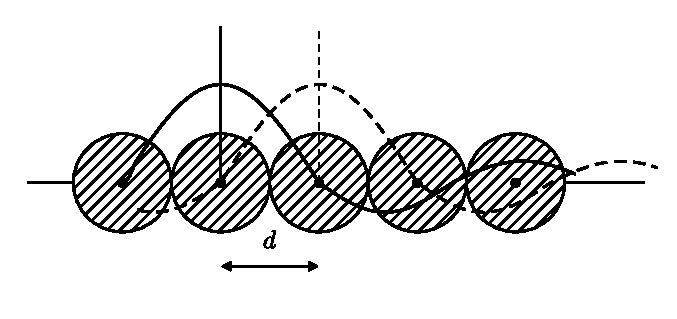
\includegraphics[width=0.72\textwidth]{fig_98.pdf}
\caption*{图 98\quad 相邻格点上的 Wannier 函数。}
\end{figure}

这样，Wannier 函数便是 Bloch 函数的一个幺正变换（unitary transformation），作为电子态的一种表示，二者在形式上等价。正如 §5.8 中所指出的，在绝缘体中——那里的电子被关联效应很好地局域化，束缚在自己的原子上——Wannier 函数或许实际上构成一种更合适的表示。然而在金属或半导体中，电子飞速穿越整个晶体，Bloch 态更适合用来描述那些粒子、准粒子、单电子激发、载流子，或者随便我们怎么称呼它们。

如果我们假定式 (1.60)

\begin{equation*}
\psi_{\mathbf{k}}(\mathbf{r}) = N^{-\frac{1}{2}}\,u(\mathbf{r})\,e^{i\mathbf{k}\cdot\mathbf{r}}
\tag{6.14}
\end{equation*}

并取周期函数 $u(\mathbf{r})$ 对一个能带中所有 Bloch 态都近似相同，那么容易证明：对于边长为 $d$ 的简立方晶格，原点处的 Wannier 函数为

\begin{equation*}
a(\mathbf{r}) = u(\mathbf{r})\,\frac{\sin(\pi x/d).\ \sin(\pi y/d).\ \sin(\pi z/d)}{(\pi x/d).\ (\pi y/d).\ (\pi z/d)}.
\tag{6.15}
\end{equation*}

这个函数在晶胞中心看起来像 $u(\mathbf{r})$，但它以逐渐衰减的振荡向外延伸得很远。这些振荡是保证正交性所必需的，却没有直接的物理意义。Wannier 函数对某些数学目的来说很方便，但无助于我们直接思考物理现象。

\section{Wannier 表象中的运动方程}

我们要为在晶格势加上外加场势中运动的电子求出含时 Schrödinger 方程的解。我们要求它满足

\begin{equation*}
(\mathcal{H}^0 + \mathcal{U})\,\psi(\mathbf{r},t) = i\hbar\,\frac{\partial\psi(\mathbf{r},t)}{\partial t},
\tag{6.16}
\end{equation*}

其中 $\mathcal{H}^0$ 是电子在完整晶格中的哈密顿量，$\mathcal{U}$ 是微扰势。

让我们试着构造一个类似 (6.7) 的解，但以 Wannier 函数作为局域函数：我们假设

\begin{equation*}
\psi(\mathbf{r},t) = \sum_{n,\boldsymbol{l}} f_n(\boldsymbol{l},t)\,a_n(\mathbf{r}-\boldsymbol{l}),
\tag{6.17}
\end{equation*}

其中每一个能带——也就是说，每一种局域 Wannier 函数——都有各自独立的包络函数。

把 (6.17) 代入 Schrödinger 方程，乘以 $a_{n'}^{*}(\mathbf{r}-\boldsymbol{l}')$，并对整个晶体积分，得到

\begin{equation*}
\sum_{n,\boldsymbol{l}} \int a_{n'}^{*}(\mathbf{r}-\boldsymbol{l}')\,(\mathcal{H}^0 + \mathcal{U})\,a_n(\mathbf{r}-\boldsymbol{l})\,f_n(\boldsymbol{l},t) = i\hbar\,\frac{\partial f_{n'}(\boldsymbol{l}',t)}{\partial t}
\tag{6.18}
\end{equation*}

（我们在右端用到了正交关系 (6.13)。）

但 Wannier 函数本身正是从无微扰晶体的方程的解导出的，即

\begin{equation*}
\mathcal{H}^0\,\psi_{\mathbf{k},n} = \mathcal{E}_n(\mathbf{k})\,\psi_{\mathbf{k},n}
\tag{6.19}
\end{equation*}

在第 $n$ 个能带中成立。把它应用于 (6.9) 与 (6.12)，得

\begin{align*}
\mathcal{H}^0\,a_n(\mathbf{r}-\boldsymbol{l}) &= \frac{1}{\sqrt{N}}\sum_{\mathbf{k}} e^{-i\mathbf{k}\cdot\boldsymbol{l}}\,\mathcal{H}^0\,\psi_{\mathbf{k},n} \\
&= \frac{1}{\sqrt{N}}\sum_{\mathbf{k}} e^{-i\mathbf{k}\cdot\boldsymbol{l}}\,\mathcal{E}_n(\mathbf{k})\,\psi_{\mathbf{k},n} \\
&= \frac{1}{N}\sum_{\mathbf{k}} e^{-i\mathbf{k}\cdot\boldsymbol{l}}\,\mathcal{E}_n(\mathbf{k})\sum_{\boldsymbol{l}'} e^{i\mathbf{k}\cdot\boldsymbol{l}'}\,a_n(\mathbf{r}-\boldsymbol{l}') \\
&= \sum_{\boldsymbol{l}'} \mathcal{E}_{n,\boldsymbol{l}-\boldsymbol{l}'}\,a_n(\mathbf{r}-\boldsymbol{l}'), \tag{6.20}
\end{align*}

其中我们\emph{定义}能量的 Fourier 变换，正如 (3.32) 中那样，即

\begin{equation*}
\mathcal{E}_{n,\boldsymbol{l}} \equiv \frac{1}{N}\sum_{\mathbf{k}} \mathcal{E}_n(\mathbf{k})\,e^{-i\mathbf{k}\cdot\boldsymbol{l}}.
\tag{6.21}
\end{equation*}

把 (6.20) 和 (6.21) 与 (3.27) 类比一番是相当有意思的。系数 $\mathcal{E}_{n,\boldsymbol{l}}$ 是晶格哈密顿量在第 $n$ 个能带中相距 $\boldsymbol{l}$ 的两个格点的 Wannier 函数之间的交叠积分（overlap integral）。Wannier 函数的正交性使这些结果严格成立，而对原子轨道来说它们只是近似的。

把 (6.20) 代入我们的运动方程 (6.18)，得

\begin{equation*}
\sum_{n,\boldsymbol{l}} \big\{\delta_{nn'}\,\mathcal{E}_{n,\boldsymbol{l}-\boldsymbol{l}'} + \mathcal{U}_{nn'}(\boldsymbol{l},\boldsymbol{l}')\big\}\,f_n(\boldsymbol{l},t) = i\hbar\,\frac{\partial f_{n'}(\boldsymbol{l}',t)}{\partial t},
\tag{6.22}
\end{equation*}

其中

\begin{equation*}
\mathcal{U}_{nn'}(\boldsymbol{l},\boldsymbol{l}') \equiv \int a_{n'}^{*}(\mathbf{r}-\boldsymbol{l}')\,\mathcal{U}(\mathbf{r})\,a_n(\mathbf{r}-\boldsymbol{l})\,\mathbf{dr}
\tag{6.23}
\end{equation*}

是微扰势在 Wannier 函数之间的一个矩阵元。

这些方程都是严格的。在作近似之前，我们还能再走一步。考虑下面这个形式化的论证：

\begin{align*}
\mathcal{E}_n(-i\nabla)\,f(\mathbf{r}) &= \sum_{\boldsymbol{l}} \mathcal{E}_{n,\boldsymbol{l}}\,e^{i\boldsymbol{l}\cdot(-i\nabla)}\,f(\mathbf{r}) \\
&= \sum_{\boldsymbol{l}} \mathcal{E}_{n,\boldsymbol{l}}\,\big[\,1 + \boldsymbol{l}\cdot\nabla + \tfrac{1}{2}(\boldsymbol{l}\cdot\nabla)^2\,\ldots\,\big]\,f(\mathbf{r}) \\
&= \sum_{\boldsymbol{l}} \mathcal{E}_{n,\boldsymbol{l}}\,\Big[\,f(\mathbf{r}) + \boldsymbol{l}\cdot\nabla f(\mathbf{r}) + \frac{1}{2}\Big\{l_x^2\,\frac{\partial^2 f(\mathbf{r})}{\partial x^2} + \ldots\Big\}\ldots\Big] \\
&= \sum_{\boldsymbol{l}} \mathcal{E}_{n,\boldsymbol{l}}\,f(\mathbf{r}+\boldsymbol{l}). \tag{6.24}
\end{align*}

在这一推演中，我们假定给定能带中的 $\mathcal{E}_n(\mathbf{k})$ 是 $\mathbf{k}$ 的连续解析函数，不靠近任何奇点或支点。我们利用 (6.21) 的逆关系来表达算符 $(-i\nabla)$ 的相应函数，即

\begin{equation*}
\mathcal{E}_n(\mathbf{k}) = \sum_{\boldsymbol{l}} \mathcal{E}_{n,\boldsymbol{l}}\,e^{i\mathbf{k}\cdot\boldsymbol{l}},
\tag{6.25}
\end{equation*}

并把指数按算符 $\nabla$ 的幂级数展开。这个级数结果就是 $f(\mathbf{r}+\boldsymbol{l})$ 的 Taylor 展开。只要 $f(\mathbf{r})$ 连续等等，结果 (6.24) 便成立。

把 (6.24) 代入 (6.22)，得

\begin{equation*}
\Big[\mathcal{E}_{n'}(-i\nabla)\,f_{n'}(\mathbf{r},t) - i\hbar\,\frac{\partial f_{n'}(\mathbf{r},t)}{\partial t}\Big]_{\mathbf{r}=\boldsymbol{l}'} + \sum_{n,\boldsymbol{l}} \mathcal{U}_{nn'}(\boldsymbol{l},\boldsymbol{l}')\,f_n(\boldsymbol{l},t) = 0.
\tag{6.26}
\end{equation*}

这个方程——在单个能带内仍然是严格的——支配着包络函数 $f_n(\mathbf{r},t)$ 的行为。它既有趣又有用，因为我们现在把这个包络函数当作 $\mathbf{r}$ 的连续函数来处理，就像一个穿越晶体传播的连续波，而不再只是把它看作仅在各格点上有定义的量。颇为笨拙的差分方程组 (6.22) 由此换成了一个微分方程。

而且，这个微分方程与含时 Schrödinger 方程颇为相似。例如，对自由电子我们有

\begin{equation*}
\mathcal{E}(\mathbf{k}) = \frac{\hbar^2 k^2}{2m},
\tag{6.27}
\end{equation*}

于是 (6.26) 变成

\begin{equation*}
\Big[-\frac{\hbar^2}{2m}\nabla^2 - i\hbar\,\frac{\partial}{\partial t}\Big]\,f_n(\mathbf{r},t) + \sum_{n,\boldsymbol{l}} \mathcal{U}_{nn'}(\boldsymbol{l},\mathbf{r})\,f_n(\boldsymbol{l},t) = 0,
\tag{6.28}
\end{equation*}

它就像普通的含时 Schrödinger 方程，其中 $f_n(\mathbf{r},t)$ 扮演着电子的普通波函数。

\section{等效哈密顿量：杂质能级}

为了最大限度地利用 (6.26)，通常要作若干近似。第一个近似是假定：只用出自单一能带的 Wannier 函数，就足以令人满意地表示运动电子。这意味着我们忽略 $n \neq n'$ 的所有矩阵元 $\mathcal{U}_{nn'}(\boldsymbol{l},\boldsymbol{l}')$。换言之，\emph{我们假定微扰不足以强到或陡峭到能引起带间跃迁。}这并不总是成立的。例如，高频电场可能引起向更高能带的光学跃迁；非常强的电场则可以导致 Zener 效应（Zener effect）（见 §6.8）。

我们还将假定，当 $\boldsymbol{l} \neq \boldsymbol{l}'$ 时 $\mathcal{U}_{nn}(\boldsymbol{l},\boldsymbol{l}')$ 可以忽略。这同样是假定\emph{微扰随晶格中的位置缓慢变化}，从而由不同格点上 Wannier 函数的正交性，(6.23) 为零。如果 $\mathcal{U}(\mathbf{r})$ 是变化迅速的函数——例如金属或半导体中杂质邻域的场——这个近似就容易导致严重的误差。

现在我们可以写出

\begin{equation*}
\mathcal{U}_{nn}(\boldsymbol{l},\boldsymbol{l}) = \big[\,\mathcal{U}(\mathbf{r})\,\big]_{\mathbf{r}=\boldsymbol{l}},
\tag{6.29}
\end{equation*}

即第 $l$ 个格点处微扰势的取值。我们的运动方程便等价于

\begin{equation*}
\Big\{\mathcal{E}_n(-i\nabla) - i\hbar\,\frac{\partial}{\partial t}\Big\}\,f_n(\mathbf{r},t) + \mathcal{U}(\mathbf{r})\,f_n(\mathbf{r},t) = 0
\tag{6.30}
\end{equation*}

并在每个格点处对 $\mathbf{r}$ 取值来计算。可以说，很自然的做法是在格点之间进行内插，把 $f_n(\mathbf{r},t)$ 当作位置的普通连续函数来处理，让它在局域势 $\mathcal{U}(\mathbf{r})$ 中扮演电子波函数的角色。

(6.30) 与我们的出发方程 (6.16) 之间的差别在于：我们无须显式地包含电子在纯粹的完整晶体晶格的场中运动时的哈密顿量 $\mathcal{H}^0$。这个算符被一个\emph{等效哈密顿量}（equivalent Hamiltonian）——即算符 $\mathcal{E}_n(-i\nabla)$——所取代。只要知道单一能带中的 $\mathcal{E}(\mathbf{k})$，就可以在完全不理会晶格势本身的情况下讨论缓慢微扰场的一切动力学效应；我们把电子当作自由的来处理，只是它的动能算符换成了 $\mathcal{E}_n(-i\nabla)$ 这一修正过的形式。

对普通的自由电子（即空晶格情形），我们已经在 (6.28) 中验证过，(6.30) 还原为普通的 Schrödinger 方程。如果像在半导体中那样，我们发现带底的能量仍是抛物型的，但形式为

\begin{equation*}
\mathcal{E}(\mathbf{k}) = \frac{\hbar^2 k^2}{2m^{*}},
\tag{6.31}
\end{equation*}

其中 $m^{*}$ 并非电子的普通质量，那么我们的等效哈密顿量就会与自由电子的相同，只是处处以 $m^{*}$ 代替 $m$。

这正是半导体中\emph{杂质能级}（impurity level）观念的核心。我们已经看到（§§4.6、5.5），像 Ge 中的 As 这样的杂质会产生一个有效场

\begin{equation*}
\mathcal{U}(\mathbf{r}) = \frac{-e^2}{\epsilon r},
\tag{6.32}
\end{equation*}

其中 $\epsilon$ 是介质的静态介电常数。如果这个场可以当作缓慢变化的场来处理，而且 (6.31) 足以恰当地描述导带底附近电子的能量，那么我们的等效 Schrödinger 方程就与氢原子的方程相同，只是以 $m^{*}$ 代替电子的质量，以 $e/\sqrt{\epsilon}$ 代替它的电荷。

这样，我们就可以搬用众所周知的氢原子能级理论。导带底算作动能的零点；在该零点之下将有位于

\begin{equation*}
W_n = -\frac{m^{*}e^{4}}{2\epsilon^{2}\hbar^{2}}\,\frac{1}{n^{2}}
\tag{6.33}
\end{equation*}

处的束缚态。但这是一个很小的能量。例如，若 $m^{*} = m/10$、$\epsilon = 10$，则该杂质能级的电离能（ionization energy）将为 $10^{-3}$ 里德伯（rydberg）。因此，它只比导带底低一点点，处在带隙之内。

我们还注意到，等效波函数（即包络函数 $f(\mathbf{r},t)$）的“Bohr 半径”被放大了 $(m\epsilon/m^{*})$ 倍，大约为 100 倍。正是这个大尺寸，使得我们用近似哈密顿量 (6.30) 去描述实际上在 $\mathbf{r}=0$ 附近变化很快的微扰 (6.32) 成为合理。

\begin{figure}[H]
\centering
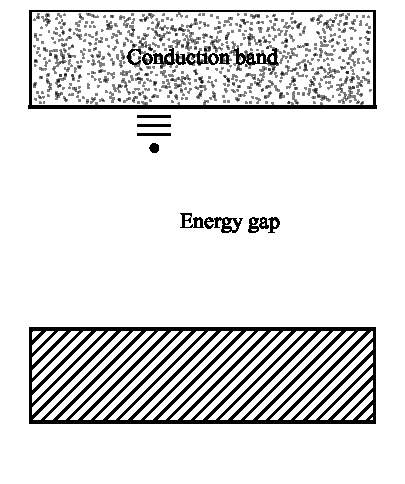
\includegraphics[width=0.72\textwidth]{fig_99.pdf}
\caption*{图 99\quad 杂质能级。}
\end{figure}

像 (6.33) 这样的能级确实已被观测到，不过理论的细节以及观测到的效应都比我们这里所述的更为复杂。例如，只有当相对浓度极低时，“杂质彼此互不影响”这一假定才是合理的。只要在 $10^{5}$ 个 Ge 或 Si 原子中所含的 As 或 Sb 原子不超过一个，邻近杂质上的电子态就必然开始交叠。虽然这些“原子”并非排列成规则晶格，但这样的集合类似于 §3.4 的紧束缚模型：各个“原子轨道”应当相互组合并展宽成一个窄带（图 100）。浓度更高时，交叠积分（参见式 (3.27)）超过杂质能级的电离能，于是这个带最终与导带底合并——事实上，杂质态本来就是从导带底引出来的。这个\emph{杂质带}（impurity band）的理论很有意思：它既是无序系统中电子态的一个极端例子，又是一个可以通过调节各种杂质的浓度来实现由绝缘导电到金属导电的 Mott 转变（§5.9）的体系。

\begin{figure}[H]
\centering
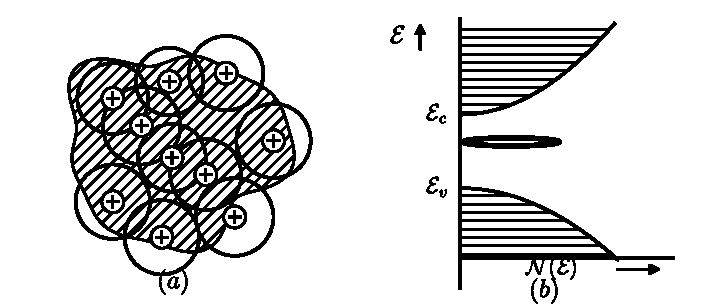
\includegraphics[width=0.72\textwidth]{fig_100.pdf}
\caption*{图 100\quad (a) 相互交叠的杂质态导致 (b) 禁带中的杂质带。}
\end{figure}

但是，在离子晶体中\emph{负离子空位}（negative ion vacancy）或 \emph{F 心}（F-centre）在这类类似的情形下，等效哈密顿量的形式体系就失效了。不难论证：在静电中性的晶格中缺少一个负离子，等价于一个局域的正电荷，它以库仑场 (6.32) 吸引一个电子。然而，传导电子的有效质量 $m^{*}$ 不够小，$\epsilon$ 也不够大，不足以支持使用类氢波函数（hydrogenic wave functions）。电子的大部分时间都待在空位的紧邻区域，在那里最好把它当作一个普通的裸粒子，在各相邻离子的静电场叠加而成的场中运动——这个势看起来就像一个没有中心奇点的平底方势阱（图 101）。这个\emph{点离子模型}（point-ion model）尽管简单，却为色心（colour centre）中电子态的理论（见 §8.5）提供了良好的定量基础；F 心就是其中最简单的例子。

\begin{figure}[H]
\centering
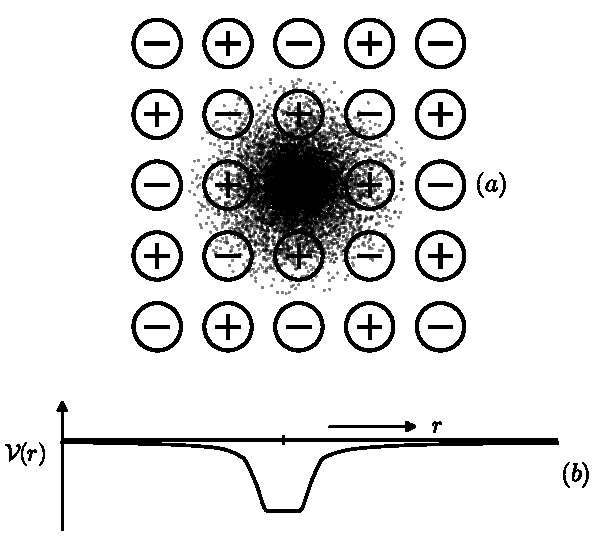
\includegraphics[width=0.72\textwidth]{fig_101.pdf}
\caption*{图 101\quad (a) F 心中的电子电荷云。(b) 点离子模型势阱。}
\end{figure}

\section{准经典动力学}

在任何涉及电子在晶格中运动的问题里，我们都可以着手去求解等效 Schrödinger 方程 (6.30)。但如果 $\mathcal{E}(\mathbf{k})$ 是 $\mathbf{k}$ 的一个复杂函数，这样做可能会导致相当棘手的数学。

应用对应原理（correspondence principle）可以避开其中大部分困难。众所周知，Schrödinger 方程的波包解与经典粒子遵循同样的轨迹，后者服从由相应的经典哈密顿量导出的运动方程。按照量子力学的Schrödinger 表述，波动方程中的哈密顿量\emph{算符}是这样得到的：在经典哈密顿量\emph{函数}中，用 $-i\hbar\nabla$ 代替经典动量变量 $\mathbf{p}$。把上述步骤反过来，我们可以在等效哈密顿量算符 $\mathcal{E}(-i\nabla)$ 中，把算符 $-i\nabla$ 换成动量变量 $\mathbf{p}/\hbar$，并把所得结果称为等效经典哈密顿量函数。于是，
\begin{equation*}
\mathcal{E}(-i\nabla)+\mathcal{U}(\mathbf{r})\;\rightarrow\;\mathcal{E}(\mathbf{p}/\hbar)+\mathcal{U}(\mathbf{r})=\mathcal{H}(\mathbf{r},\mathbf{p}). \tag{6.34}
\end{equation*}
我们的电子波包将表现得如同经典点粒子，服从由这个哈密顿量函数生成的运动方程。

Hamilton 方程可以符号式地写成
\begin{equation*}
\dot{\mathbf{r}}=\frac{\partial\mathcal{H}}{\partial\mathbf{p}},\quad \dot{\mathbf{p}}=-\frac{\partial\mathcal{H}}{\partial\mathbf{r}}. \tag{6.35}
\end{equation*}
其中第一式便成为一个关于速度的方程，
\begin{align*}
\mathbf{v}&=\frac{\partial\mathcal{H}}{\partial\mathbf{p}}=\frac{\partial}{\partial\mathbf{p}}\bigl\{\mathcal{E}(\mathbf{p}/\hbar)+\mathcal{U}(\mathbf{r})\bigr\}\\
&=\frac{\partial\mathcal{E}(\mathbf{p}/\hbar)}{\partial\mathbf{p}}\\
&=\frac{1}{\hbar}\frac{\partial\mathcal{E}(\mathbf{k})}{\partial\mathbf{k}}. \tag{6.36}
\end{align*}
用我们更常用的变量 $\mathbf{k}$ 表出。这正是式 (6.2)，至此终于得到证明。我们看到
\begin{equation*}
\hbar\mathbf{k}=\mathbf{p} \tag{6.37}
\end{equation*}
的确扮演着经典动量的角色；尽管它并不是一个唯一确定的变量，它却标记着波包恰好主要集中于其上的那个“态”。

Hamilton 方程中的第二式可以写成
\begin{equation*}
\hbar\dot{\mathbf{k}}=-\frac{\partial\mathcal{H}}{\partial\mathbf{r}}=-\nabla\mathcal{U}(\mathbf{r}). \tag{6.38}
\end{equation*}
但如果 $\mathcal{U}(\mathbf{r})$ 譬如说是电子在固定静电场中的势能，那么右端就简单地是作用在电子上的经典力。例如，在电场 $\mathbf{E}$ 中，我们有
\begin{equation*}
\hbar\dot{\mathbf{k}}=e\mathbf{E}. \tag{6.39}
\end{equation*}
这就证明了我们的第二条动力学定律 (6.5)。变量 $\hbar\mathbf{k}$ 之所以扮演动量的角色，在于恒力的效果是使 $\hbar\mathbf{k}$ 以恒定速率增大。这里再次看到，$\mathbf{k}$ 不唯一这一事实并无妨碍，因为进入这些方程的只是它的导数。

至于磁场 $\mathbf{H}$ 的效应，我们假定 \emph{Lorentz 力}（Lorentz force）方程成立，即
\begin{equation*}
\hbar\dot{\mathbf{k}}=e\Bigl(\mathbf{E}+\frac{1}{c}\,\mathbf{v}\wedge\mathbf{H}\Bigr), \tag{6.40}
\end{equation*}
其中 $\mathbf{v}$ 是波包的速度，由式 (6.36) 算得；$c$ 是光速。这个公式是从式 (6.39) 类比而来的，但它的正当推导要困难得多。人们相信，直到非常强的磁场它都成立得相当好（见 §9.8）。

\section{质量张量：电子与空穴}

让我们把运动学方程和动力学方程 (6.36) 与 (6.39) 结合起来，计算一个电子的\emph{加速度}，
\begin{align*}
\dot{\mathbf{v}}&=\frac{\partial}{\partial t}\biggl\{\frac{1}{\hbar}\frac{\partial\mathcal{E}(\mathbf{k})}{\partial\mathbf{k}}\biggr\}\\
&=\frac{1}{\hbar}\frac{\partial}{\partial\mathbf{k}}\biggl\{\frac{1}{\hbar}\frac{\partial\mathcal{E}(\mathbf{k})}{\partial\mathbf{k}}\biggr\}\cdot\frac{\hbar\,\partial\mathbf{k}}{\partial t}\\
&=\frac{1}{\hbar^{2}}\frac{\partial^{2}\mathcal{E}(\mathbf{k})}{\partial\mathbf{k}\,\partial\mathbf{k}}\cdot e\mathbf{E}. \tag{6.41}
\end{align*}
\begin{figure}[H]
\centering
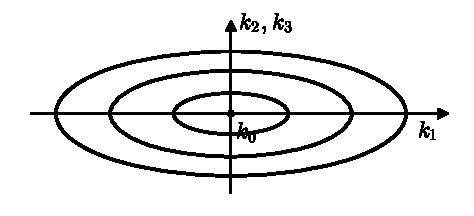
\includegraphics[width=0.72\textwidth]{fig_102.pdf}
\caption*{图 102\quad 质量沿"谷"的方向很大。}
\end{figure}

若把它与常规的 Newton 方程
\begin{equation*}
m\dot{\mathbf{v}}=e\mathbf{E}, \tag{6.42}
\end{equation*}
相比较，我们看到电子质量的等效物如今是一个张量的逆：
\begin{equation*}
\frac{1}{m}\;\rightarrow\;\frac{1}{\hbar^{2}}\frac{\partial^{2}\mathcal{E}(\mathbf{k})}{\partial\mathbf{k}\,\partial\mathbf{k}}. \tag{6.43}
\end{equation*}
这个张量是最接近于电子的动力学质量的等效物。例如，在半导体中，能量面可以具有 (4.35) 的形式，即
\begin{equation*}
\mathcal{E}(\mathbf{k})=\frac{\hbar^{2}k_{1}^{2}}{2m_{1}}+\frac{\hbar^{2}k_{2}^{2}}{2m_{2}}+\frac{\hbar^{2}k_{3}^{2}}{2m_{3}} \tag{6.44}
\end{equation*}
它参照某个局域主轴系写出。电场在不同方向上对电子加速的效果于是将大不相同。如果能量面沿 $k_{1}$ 方向拉长成椭球，即若 $m_{1}\gg m_{2}\sim m_{3}$，那么沿“谷”方向测得的质量就显得比横向方向大得多。在计算各种态对电子平均迁移率的贡献时，这一点很重要。施主杂质能级的简单类氢公式 (6.33) 也必须加以修正，以顾及每个谷的等效哈密顿量的各向异性，以及许多半导体导带底处同一能量诸谷的多重性。

\emph{逆质量张量}（inverse mass tensor）不一定是正定的。在（如贵金属 Cu、Ag、Au 中）费米面与区边界相接触之处，我们可以近似地把它表成 (6.44) 的形式，但取 $m_{3}$ 为\emph{负}，从而给出双曲型能量面（在 §3.3 的重复区图式中，可以让它们恰好穿过区边界）。从经典的观点看，$\mathbf{k}$ 空间中这样一点上电子的动力学行为会显得非常奇怪。

它们被来自区边界的强 Bragg 反射深刻地改变。实际上，电子倾向于沿着晶格平面传播，仿佛穿过一系列波导一般。

\begin{figure}[H]
\centering
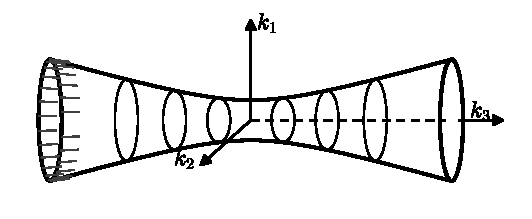
\includegraphics[width=0.72\textwidth]{fig_103.pdf}
\caption*{图 103\quad 双曲面状能量面（"颈"）。}
\end{figure}

\begin{figure}[H]
\centering
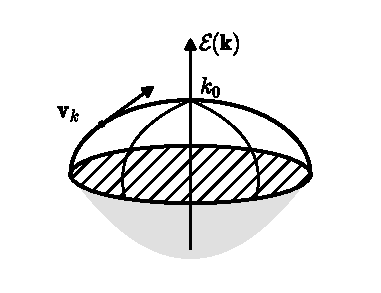
\includegraphics[width=0.72\textwidth]{fig_104.pdf}
\caption*{图 104\quad 近满带带顶处的"空穴袋"。}
\end{figure}

更常见的情形是像半导体或半金属中那样的\emph{近满带}（nearly full band）。由于 $\mathcal{E}(\mathbf{k})$ 在重复区中是连续的周期函数，被占据的态将几乎一直填充到 $\mathcal{E}(\mathbf{k})$ 的某个明确的极大值。若这个极大值出现在 $\mathbf{k}_{0}$ 处，那么作为 $\mathcal{E}(\mathbf{k})$ 的梯度的 $\mathbf{v}_{\mathbf{k}}$ 在 $\mathbf{k}=\mathbf{k}_{0}$ 处为零，而且在 $\mathbf{k}_{0}$ 附近的一切方向上，$\partial^{2}\mathcal{E}/\partial\mathbf{k}\,\partial\mathbf{k}$ 的主分量都是\emph{负}的。

具有\emph{负有效质量}（negative effective mass）的电子，其性质与寻常粒子相差太远，以至于更便当的做法是把论证反过来说，去讨论满带中少数\emph{空穴}（hole）的性质。我们在 §4.6 中已经指出，这种空穴的数目可以相当简单地用 费米–狄拉克 统计算出，只需把能量\emph{向下}量度；现在我们要证明，如果把空穴当作\emph{带正电}的粒子来处理，同一个能量约定将以经典上可理解的形式描述它们的动力学性质。

\begin{figure}[H]
\centering
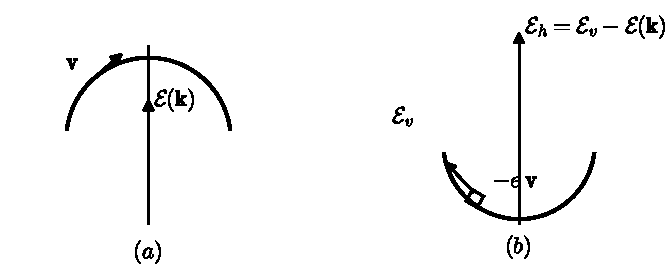
\includegraphics[width=0.72\textwidth]{fig_105.pdf}
\caption*{图 105\quad (a) 电子分布中的一个空隙。(b) 相应的"空穴"，能量标度已倒置。}
\end{figure}

我们首先注意到，“处于态 $\mathbf{k}$ 的空穴”必须由一个行列式来描述，这个行列式包含带中除态 $\psi_{\mathbf{k}}$ 之外的所有波函数。我们还可以更进一步，实际构造出这种行列式的波包。但需要注意的要点是，空穴的“速度”与那个缺失态的速度相同；波包将以与空穴两侧邻居相同的速率被携带着通过空间：
\begin{equation*}
\mathbf{v}_{\mathbf{k}}=\frac{1}{\hbar}\frac{\partial\mathcal{E}(\mathbf{k})}{\partial\mathbf{k}}. \tag{6.45}
\end{equation*}
现在来考虑与一个空穴相联系的电流。满带的电流为零。处于态 $\mathbf{k}$ 的一个电子的电流是 $-|e|\mathbf{v}_{\mathbf{k}}$。因此，缺了一个电子的满带，其电流必定是
\begin{equation*}
\mathbf{J}_{h}=0-(-|e|\mathbf{v}_{\mathbf{k}})=|e|\mathbf{v}_{\mathbf{k}}. \tag{6.46}
\end{equation*}
可见空穴的行为就像一个\emph{带正电的粒子}（positively charged particle）。

同样，空穴的动力学必定与它两侧各态的动力学相同。速度将以式 (6.41) 所定义的速率改变。若用电流来表述，我们有
\begin{align*}
|e|\dot{\mathbf{v}}&=|e|\,\frac{1}{\hbar^{2}}\frac{\partial^{2}\mathcal{E}(\mathbf{k})}{\partial\mathbf{k}\,\partial\mathbf{k}}\cdot(-|e|)\mathbf{E}\\
&=|e|\biggl\{-\frac{1}{\hbar^{2}}\frac{\partial^{2}\mathcal{E}(\mathbf{k})}{\partial\mathbf{k}\,\partial\mathbf{k}}\biggr\}\cdot|e|\mathbf{E}, \tag{6.47}
\end{align*}
这就是一个电荷为正、大小为 $|e|$ 的粒子的加速度方程，只是其质量为 $m^{*}$，其中
\begin{equation*}
\frac{1}{m^{*}}\sim-\frac{1}{\hbar^{2}}\frac{\partial^{2}\mathcal{E}(\mathbf{k})}{\partial\mathbf{k}\,\partial\mathbf{k}}. \tag{6.48}
\end{equation*}
但由于我们是在带顶附近，曲率的所有分量都是负的，所以 $m^{*}$ 现在是一个正量。于是，空穴的动力学性质未必各向同性，但它们基本上就是具有正质量的经典粒子的动力学性质。

\begin{figure}[H]
\centering
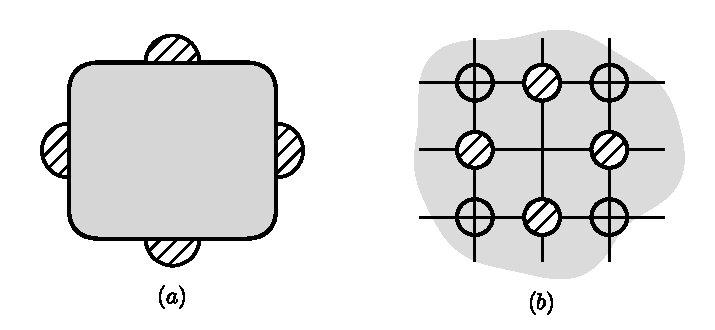
\includegraphics[width=0.72\textwidth]{fig_106.pdf}
\caption*{图 106\quad 小重叠的能带：(a) 扩展区图式；(b) 重复区图式。}
\end{figure}

价带带顶的空穴导电，当然是半导体的一个特征性质。在 Si 和 Ge 中，区中心的能量面被自旋–轨道相互作用所分裂（参看图 66），我们实际上可以观察到“轻”“重”两种空穴，它们对应于 $\mathcal{E}(\mathbf{k})$ 的两支，曲率不同而在极大值处相接触。

\begin{figure}[H]
\centering
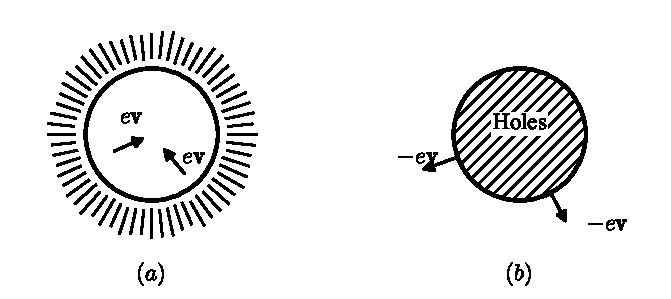
\includegraphics[width=0.72\textwidth]{fig_107.pdf}
\caption*{图 107\quad (a) 电子分布中的一个空球变成 (b) 一个"空穴球"。}
\end{figure}

显然，当我们离开极大值位置时，空穴的速度会增大，也就是说，随 $\mathcal{E}(\mathbf{k})$ 的减小而增大。同样方便的做法是把空穴的动能看成 $\mathcal{E}_{h}=\mathcal{E}_{v}-\mathcal{E}(\mathbf{k})$，即从价带顶这个原点向外增大。这就是 §4.6 中引入的约定。

对于每单位晶胞含偶数个电子的半金属（如 Bi），如果存在向更高能带的小重叠、有少量电子溢了出去，我们也会遇到类似的情形。这时在近满带中会留下等数目的空穴——它们将由费米面的若干碎片包住，这些碎片可以像 §3.3 中那样在重复区图式中拼合成闭合曲面。把这样一个空穴\emph{袋}（pocket）设想成少数几个带正电的粒子、其速度矢量由中心指向外，要比讨论一个电子的费米面（其速度矢量画成指向未占据空间区域的内部）来得容易。然而应当强调，把态分类为“空穴”和“电子”的做法可能失效——例如在图 103 的“颈”上。

空穴在离子晶体中能否像自由粒子那样运动，是值得怀疑的。相邻离子上价轨道之间的小重叠意味着价带非常窄（§3.4），有效质量相应地很大。这似乎允许空穴发生\emph{自陷}（self-trapping）——例如在 KCl 中，空穴定域在两个 Cl$^{-}$ 离子之间，这两个离子被拉近而形成一个稳定的 \emph{V 心}（V centre），只有靠热激发才能把空穴从中释放出来。这样的\emph{小极化子}（small polaron）（§8.3）对晶格的颗粒性如此敏感，以至于只能靠从一个晶胞到另一个晶胞的“跳跃”来移动。由于这个原因，“价带”的概念在离子晶体中没有什么意义（§4.2）。

\section{激子}

存在两种载流子，电荷相反，但其他方面的性质基本上相似——这一点处于半导体应用物理的核心。我们在 §4.6 中已经证明，如何通过掺入受主杂质把空穴的数目增加到任意想要的数量，做成 \emph{p} 型样品。

\begin{figure}[H]
\centering
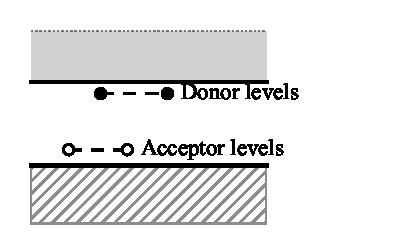
\includegraphics[width=0.72\textwidth]{fig_108.pdf}
\caption*{图 108\quad 半导体中的杂质能级。}
\end{figure}

对于施主杂质，我们在 §6.4 中已经看到：由于带电杂质对额外电子的吸引，会形成正好位于导带底之下的杂质能级。对于受主杂质有一个完全等效的理论：受主杂质带负电（因为它们必须再接纳第四个价电子以维持键结构），因此吸引的是空穴。其效果是在空穴动能零点之下不远处为空穴产生束缚态——也就是说，在价带顶之上不远处。这种\emph{受主能级}（acceptor level）的“电离能”可以完全像式 (6.33) 那样近似地算出——尽管这里又出现了同样的假设，即 $\mathcal{E}(\mathbf{k})$ 是像 (6.31) 倒置过来那样的简单二次函数，这可能又过于天真。

在一个\emph{补偿样品}（compensated sample）中，施主和受主杂质都有相当的数量，一些电子可以从施主能级“落下”去，同受主上的空穴湮灭。正如式 (4.42) 中指出的，载流子的净数目及其符号将是差 $N_{d}-N_{a}$。然而值得指出的是，“腾空”了的杂质并不是电中性的客体；施主将带正电，受主将带负电，因此它们会吸引或排斥余下的载流子。

假设我们有一块本征半导体，或者一块补偿得如此精心、以致电子和空穴的数目
由热激发公式 (4.39) 给出，而且几乎相等。这两种粒子电荷相反——所以它们彼此吸引。我们可以建立类氢的波函数，让电子和空穴绕着它们共同的质心旋转；这一对粒子的能量降低将具有与 (6.33) 相同的形式，只是 $m^{*}$ 如今应取为约化有效质量。

\begin{figure}[H]
\centering
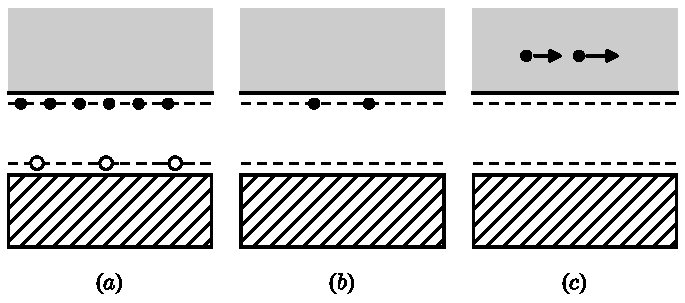
\includegraphics[width=0.72\textwidth]{fig_109.pdf}
\caption*{图 109\quad (a) 被电子和空穴占据的施主能级与受主能级。(b) 电子与空穴结合。(c) 多余的电子被热激发进入导带。}
\end{figure}

这意味着，我们有一个略低于导带底的电子能级，与一个恰好在价带之上的空穴能级相联系——事实上，是整整一系列这样的能级，对应于类氢态的不同量子数——确切地说，是整整一条\emph{激子态}（exciton state）的带，对应于电子–空穴对共同质心的运动动能的叠加（图 110、111(a)）。

思考激子的另一种方式是借助受激原子。原子或离子上的一个电子被提升到某个激发态，譬如说 $\phi_{e}(\mathbf{r})$。于是我们构造一个如下形式的 Bloch 函数
\begin{equation*}
\psi_{\mathbf{k}}=\sum_{l}e^{i\mathbf{k}\cdot l}\,\phi_{e}(\mathbf{r}-l) \tag{6.49}
\end{equation*}
以使这个激发能在晶体中传播（图 111(b)）。乍一看，这似乎不过是导带中的一个态。但我们据以导出这一论证的紧束缚法（§3.4）是单电子理论；它没有考虑电子–电子相互作用。激子态比 (6.49) 更复杂：这个运动的电子随身携带着价带中其他电子的一种局域极化——换句话说，它随身拖着自己的空穴。因此，要把这对电子–空穴分开成独立的载流子，还需要额外的一小份能量。

\begin{figure}[H]
\centering
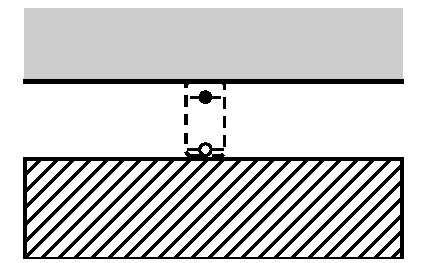
\includegraphics[width=0.72\textwidth]{fig_110.pdf}
\caption*{图 110\quad 激子态。}
\end{figure}

\begin{figure}[H]
\centering
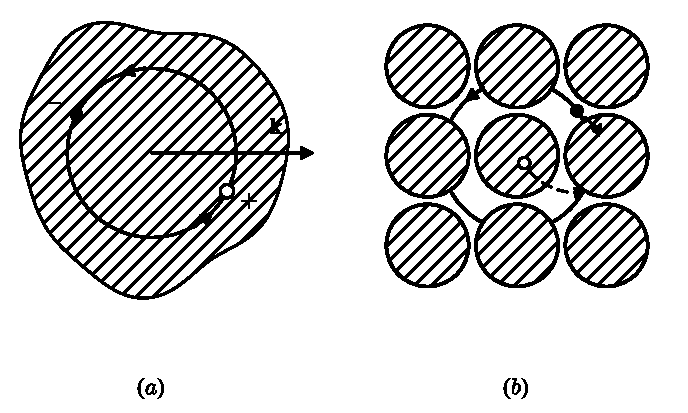
\includegraphics[width=0.72\textwidth]{fig_111.pdf}
\caption*{图 111\quad (a) Wannier 激子。(b) Frenkel 激子。}
\end{figure}

虽然激子的这两种描述实质上是等价的，但它们各自的实际适用范围不同。在半导体中，载流子很轻、介电常数很高，\emph{Wannier 激子}（Wannier exciton）的那种扩展的类氢轨道是较好的近似；在分子晶体（如固态氩或蒽）中，从\emph{Frenkel 激子}（Frenkel exciton）模型出发更为准确，这种激子的波函数大部分位于单个晶胞之内。在 NaCl 这类离子晶体中，激子的大小居中，用“一个电子从 Cl$^{-}$ 离子转移到邻近的 Na$^{+}$ 格点”来描述就相当不错。

在半导体和绝缘体的光学光谱中可以探测到激子谱线（§8.5）；但由于这种激发是电中性的，它对电导没有直接贡献。激子虽然是可移动的，并且原则上应当能够把能量输运着穿过晶体，但要在实验上演示这一现象并不容易。

\begin{figure}[H]
\centering
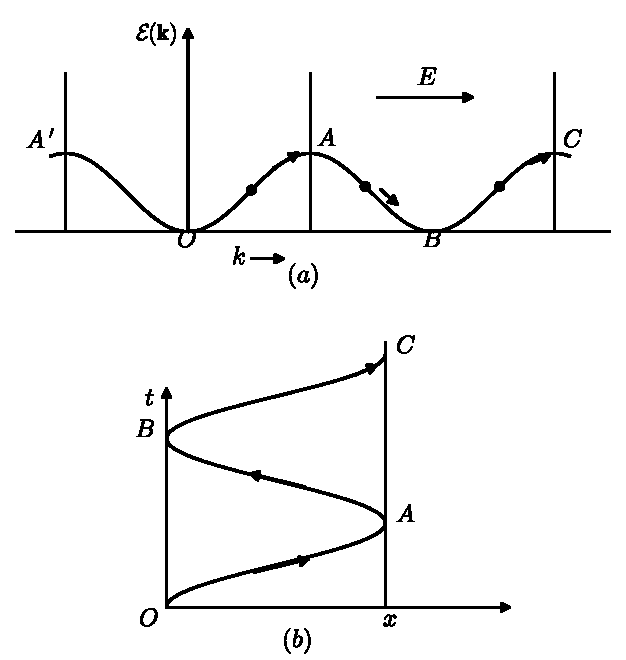
\includegraphics[width=0.72\textwidth]{fig_112.pdf}
\caption*{图 112\quad 电子在一维电场中运动。(a) $k$ 空间中的轨迹。(b) 实空间中的路径。}
\end{figure}

\section{Zener 击穿：隧穿}

§6.4 中阐述的等效哈密顿量理论，依赖于可以忽略带间跃迁这一假设。这只有在电场不太强时才成立；我们必须能够以不同能带的 Wannier 函数相互正交为理由，略去如下形式的矩阵元
\begin{equation*}
\mathcal{U}_{nn'}(l,l)=\int a^{*}_{n'}(\mathbf{r}-l)\,\mathcal{U}(\mathbf{r})\,a_{n}(\mathbf{r}-l)\,\mathrm{d}\mathbf{r}, \tag{6.50}
\end{equation*}
但如果 $\mathcal{U}(\mathbf{r})$ 随 $\mathbf{r}$ 快速变化，矩阵元 (6.50) 就未必定会为零。从纯数学的观点看，显然带间跃迁的概率将取决于 $\nabla\mathcal{U}$ 的大小。

我们想必能够由 §6.4 的表述出发来计算这个概率。但换一个更“物理的”角度来看待这一现象要容易些。让我们先考虑一个电子在弱电场中会遇到什么情况。如果电子是自由的，它就会被不断地加速，速度无限增大，一路前进，直到被散射，或者跑出样品。

但假定电子处在单一的一条简单能带中——我们可以设想一个一维模型，电场沿 $x$ 轴。代表点便稳稳地前进，从 $O$ 到 $A$。这与 $A'$ 等价——所以我们可以让它突然跳回那里——或者，采用 §3.3 的重复区图式，我们可以看到它沿周期曲线 $OABC$ 等等上下往复运动。

\begin{figure}[H]
\centering
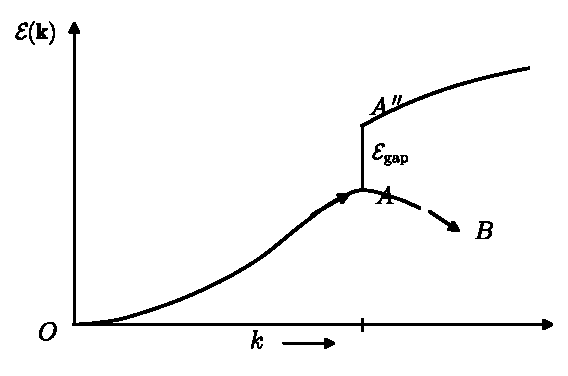
\includegraphics[width=0.72\textwidth]{fig_113.pdf}
\caption*{图 113\quad 电子不是继续走向 $B$，而是可能“跳”过带隙到达 $A''$。}
\end{figure}

在实空间中，电子从 $O$ 出发被加速，但当它接近 $A$ 时开始减慢，然后反向运动，直到它到达 $B$，再次被加速，如此往复。在 $A$ 处发生 Bragg 反射；电子不能进入 $A$ 以外的区域，因为它的能量将落入能隙之中。电子被限制在 $x$ 轴的一个有限范围内。

但现在假定还有另一条能带，其最低点 $A''$ 位于 $A$ 之上能量 $\mathcal{E}_{\mathrm{gap}}$ 处。电子总有这种可能：它从电场获得太多的能量，以至于从 $A$ 跃迁到 $A''$（译注：原文印作 to $A$ from $A''$，当为排印倒置）。

为看出这确实是可能的，设电场为恒定的。我们可以沿 $x$ 轴画出电子从电场获得的能量 $eEx$。设电子已到达较低能带顶部的 $A$ 点。那么通常它将被反射回去。但如果它能再走过一段距离
\begin{equation*}
d=\frac{\mathcal{E}_{\mathrm{gap}}}{eE}, \tag{6.51}
\end{equation*}
到达 $A''$ 点，它就已从电场获得了足以越过带隙的能量（图 114）。

\begin{figure}[H]
\centering
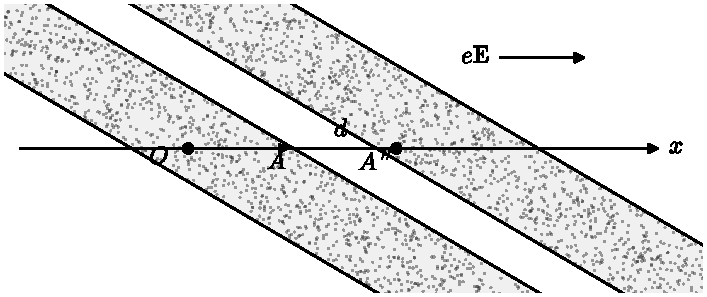
\includegraphics[width=0.72\textwidth]{fig_114.pdf}
\caption*{图 114\quad 被强电场倾斜的能带。}
\end{figure}

\begin{figure}[H]
\centering
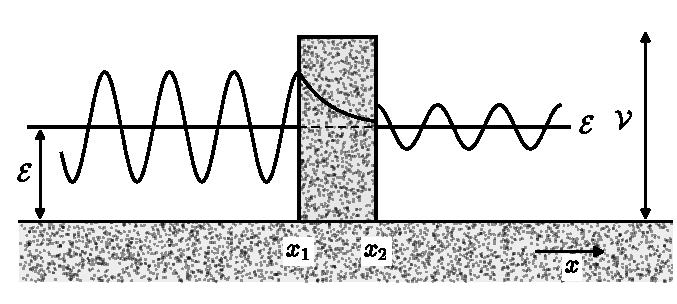
\includegraphics[width=0.72\textwidth]{fig_115.pdf}
\caption*{图 115\quad 穿过势垒的隧穿。}
\end{figure}

这本质上是一个\emph{隧穿}（tunnelling）问题。电子必须穿透一个禁戒区域。在传统的隧穿问题中，势垒是这样一个区域：势能 $\mathcal{V}$ 大于电子在自由空间中的总能量 $\mathcal{E}$，因而在势垒内部电子的动能将是负的。从量子力学上看，这意味着电子波函数获得一个实的指数因子
\begin{equation*}
\psi=\psi_{0}e^{-\beta x}, \tag{6.52}
\end{equation*}
其中
\begin{equation*}
\beta^{2}=\mathcal{V}-\mathcal{E}. \tag{6.53}
\end{equation*}
如果 $\mathcal{V}$ 是 $x$ 的函数，我们可以用 W.K.B. 方法导出跃迁概率，即透射与反射之比，其形式为
\begin{equation*}
P=\exp\Biggl\{-2\int_{x_{1}}^{x_{2}}\beta(x)\,\mathrm{d}x\Biggr\}, \tag{6.54}
\end{equation*}
其中 $x_{1}$ 和 $x_{2}$ 是势垒区域的边界，因子 2 来自把波函数平方以得到概率密度。

要把这一论证用到我们眼下的问题上，我们需要考虑能隙中电子波函数的性质。这是我们此前未曾考虑过的一点。偏微分方程
\begin{equation*}
-\frac{\hbar^{2}}{2m}\nabla^{2}\psi+\bigl\{\mathcal{V}(\mathbf{r})-\mathcal{E}\bigr\}\psi=0 \tag{6.55}
\end{equation*}
对任何 $\mathcal{E}$ 值都有解，即使当 $\mathcal{V}(\mathbf{r})$ 是满足
\begin{equation*}
\mathcal{V}(\mathbf{r}+l)=\mathcal{V}(\mathbf{r}), \tag{6.56}
\end{equation*}
的周期势时也是如此；只不过这些解不满足 Bloch 条件，因而不能作为本征函数去配合周期边界条件。

不过，我们并没有理由不采用 §3.2 中那样的势的 Fourier 分析，并尝试如下形式的解
\begin{equation*}
\psi=\sum_{\mathbf{g}}\alpha_{\mathbf{k}-\mathbf{g}}\,e^{i(\mathbf{k}-\mathbf{g})\cdot\mathbf{r}}, \tag{6.57}
\end{equation*}
只是让 $\mathbf{k}$ 的分量取复数值。我们将得到与 (3.14) 同样的系数线性方程组——只是必须把
\begin{equation*}
\mathcal{E}^{0}_{\mathbf{k}-\mathbf{g}}\equiv\frac{\hbar^{2}}{2m}(\mathbf{k}-\mathbf{g})^{2} \tag{6.58}
\end{equation*}
显式地写出来，因为它严格说来已不再是“未微扰能量”，而不过是 $(-\hbar^{2}/2m)\nabla^{2}$ 作用于 (6.57) 中各项的结果。

让我们考察一个一维模型中能隙附近的区域，即 $\mathbf{k}$ 位于与波矢
\begin{equation*}
\tfrac{1}{2}G=\frac{\pi}{a} \tag{6.59}
\end{equation*}
相应的区边界邻域的情形，此处晶面与电场垂直，其间距为 $a$。对自由电子，能量本应是
\begin{equation*}
\mathcal{E}^{0}=\frac{\hbar^{2}}{2m}\bigl(\tfrac{1}{2}G\bigr)^{2} \tag{6.60}
\end{equation*}
但正如 (3.16) 中那样，由于存在微扰 $\mathcal{V}_{G}$，我们必须求解行列式方程
\begin{equation*}
\biggl\{\frac{\hbar^{2}}{2m}k^{2}-\mathcal{E}\biggr\}\biggl\{\frac{\hbar^{2}}{2m}(k-G)^{2}-\mathcal{E}\biggr\}=|\mathcal{V}_{G}|^{2} \tag{6.61}
\end{equation*}
正如我们在 (3.19) 和 (3.20) 中看到的那样，若 $k$ 为实数，则此方程在能隙内没有 $\mathcal{E}$ 的根，也就是说，在
\begin{equation*}
\mathcal{E}^{0}-|\mathcal{V}_{G}|<\mathcal{E}<\mathcal{E}^{0}+|\mathcal{V}_{G}|. \tag{6.62}
\end{equation*}
的范围内无根。

但现在我们把 $\mathcal{E}$ 当作一个任意参量，转而求解 $k$。若写成
\begin{equation*}
k=\tfrac{1}{2}G+\kappa,\qquad\mathcal{E}=\mathcal{E}^{0}+\epsilon, \tag{6.63}
\end{equation*}
其中 $\kappa$ 和 $\epsilon$ 设为小量，则我们求得一个近似解
\begin{equation*}
\kappa^{2}\approx\frac{2m}{\hbar^{2}}\biggl[\frac{\epsilon^{2}-|\mathcal{V}_{G}|^{2}}{4\mathcal{E}^{0}}\biggr]. \tag{6.64}
\end{equation*}

显而易见，若 $|\epsilon|<|\mathcal{V}_{G}|$，则 $\kappa$ 将是纯虚数——也就是说，按 (6.62) 与 (6.63)，\emph{能量处在能隙内的电子，其波函数含有一个实的指数因子}。这完全是 Schrödinger 方程的一个正当的解——但通常在物理上无关紧要，因为在大晶体整个宽度上无法使它配合周期边界条件或其他简单边界条件。电子根本无法在固体中传播任何距离。周期系统中波函数的这种普遍性质，已经在频率位于声子谱之外的晶格振动的情形（§2.12）中指出过。

回到我们的隧穿问题，我们看到：令 (6.64) 中系数 $\beta$ 等于 $\kappa$ 的虚部，便可以用 (6.54) 来计算穿过禁戒区的透射。如果电场使电子能量在跨越禁戒区时线性增大，即 $\epsilon$ 正比于离开势垒中心（势垒总宽度为 $d$）的距离 $x$，那么我们有
\begin{equation*}
\beta(x)=\frac{|\mathcal{V}_{G}|}{2\mathcal{E}^{0}}\bigl(\tfrac{1}{2}G\bigr)\biggl(1-\frac{4x^{2}}{d^{2}}\biggr)^{\frac{1}{2}},
\end{equation*}
积分后得
\begin{align*}
P&=\exp-\biggl\{\frac{\pi d\,|\mathcal{V}_{G}|\,(\tfrac{1}{2}G)}{2\mathcal{E}^{0}}\biggr\}\\
&=\exp-\biggl\{\frac{\pi^{2}}{4}\,\frac{\mathcal{E}_{\mathrm{gap}}^{2}}{\mathcal{E}^{0}eEa}\biggr\}, \tag{6.65}
\end{align*}
这里用到了 (6.51)、(6.59)，以及 $2|\mathcal{V}_{G}|$ 即能隙宽度这一事实。

这个公式表明，如果电场 $E$ 强到电子在走过一个晶格间距 $a$ 内就能获得带隙能量的 $\mathcal{E}_{\mathrm{gap}}/\mathcal{E}^{0}$ 份额，就应当发生 Zener 击穿。然而，这一效应在实践中能否观察到尚不确定，因为它会被其他更复杂的现象所掩盖，例如\emph{雪崩击穿}（avalanche breakdown），即在由高能电子或空穴组成的电流中通过使杂质能级电离而令载流子倍增。

\begin{figure}[H]
\centering
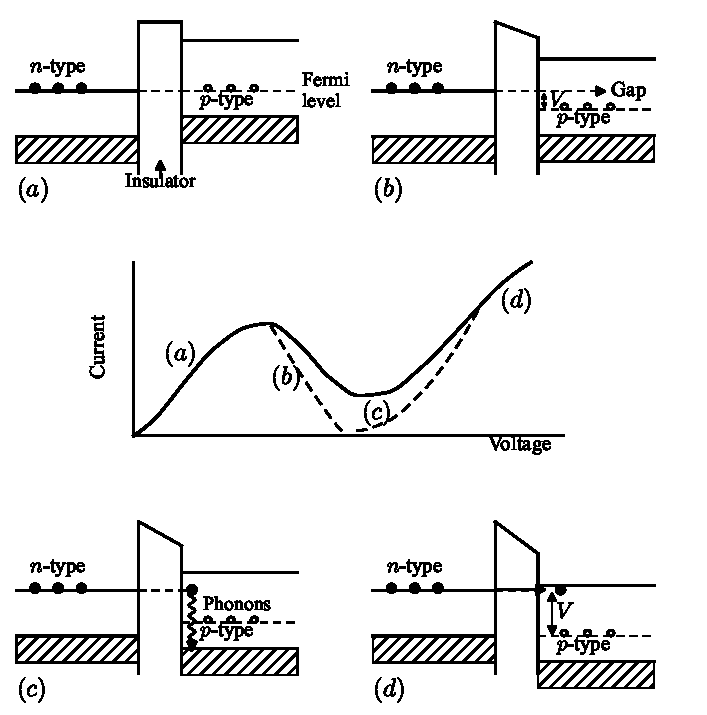
\includegraphics[width=0.72\textwidth]{fig_116.pdf}
\caption*{图 116\quad 隧道二极管特性：(a) 近零偏压；(b) 隧穿入带隙；(c) 声子辅助隧穿；(d) 少数载流子注入。}
\end{figure}

一个非常类似的效应出现在\emph{隧道二极管}或 \emph{Esaki 二极管}（Esaki diode）中：在分隔重掺杂 \emph{p} 型与 \emph{n} 型材料的一层薄绝缘膜两端加上外电场。隧穿速率主要由势垒的厚度和性质决定，但也受载流子所要进入的能带中可资利用的态密度的调制——而态密度对于电子被外加电场携带着越过禁戒区时所到达的确切能量颇为敏感。

例如在零偏压下（图 116(a)），势垒两侧的费米能级必须相同（§4.6），于是一个小的“正向”电压会使 \emph{n} 型区的电子隧穿过来，与 \emph{p} 型材料中的空穴相遇而复合，从而使电流得以流动。但势垒两侧更大的电压差会把载流子从一侧驱入另一侧的带隙之中，在那里它们无法传播（图 116(b)）。于是电流下降——但不降至零，因为载流子可以通过与声子的相互作用损失能量（\emph{声子辅助隧穿}（phonon-assisted tunnelling），图 116(c)）。与光子类似的一个效应在光学上表现为 \emph{Franz--Keldysh 效应}（Franz--Keldysh effect）。当然，在更大的电压下，隧穿之后态又变得可资利用了（图 116(d)），于是随着\emph{少数载流子}（minority carriers）的注入——即电子注入 \emph{p} 型材料、空穴注入 \emph{n} 型材料——电流再度上升。

超导体之间的结的行为与此类似，而且还表现出\emph{相干隧穿}（coherent tunnelling）现象，这将在 §11.10 中讨论。

\section{表面上的电子}

第 3 章中讨论的电子波函数被假定满足循环边界条件 (1.76)，仿佛深处大晶体内部。那么在表面附近会发生什么呢？

首先，我们需要对表面各层中原子、离子和电子密度的分布建立某种模型。我们一般可以假定势有一个抬升——即\emph{功函数}（work function）（图 117），说的是把一个电子从体材料的费米能级带到离表面相当远处所需的能量提升——但要计算所需爬越的势垒的确切形式却极其困难。即使所有化学杂质都已清除——这是一项艰巨的技术任务——仍可能有结构重排和电子密度的复杂移动，其起因是未饱和的化学键、镜像力等等。

\begin{figure}[H]
\centering
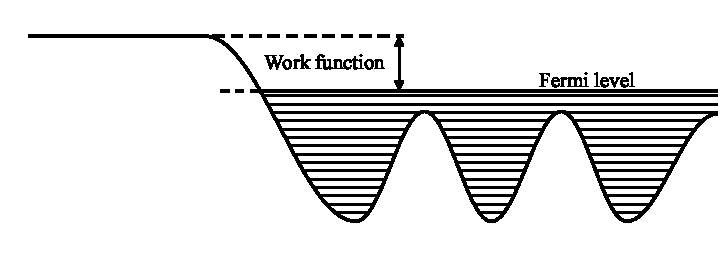
\includegraphics[width=0.72\textwidth]{fig_117.pdf}
\caption*{图 117\quad 表面处的功函数势垒。}
\end{figure}

然而，容易证明，普通 Bloch 态的分布几乎不受表面条件的影响。一个在晶体外呈指数衰减的波函数，可以同一个本来就近乎简并的内部波的组合相匹配，能量只需移动一个无穷小量。匹配的确切细节将依赖于势垒的精确形状，但这对体材料的能带结构等没有影响。

但要考虑能量处在带隙内的电子。如上一节所示，晶体\emph{内部} Schrödinger 方程的解同样由距离的指数函数 (6.52) 主导。设此函数是向晶体内部衰减的，然后我们成功地把它在振幅和梯度上同一个简单指数函数匹配起来——后者描写一个试图穿过表面势垒逃逸出去的电子。这样我们就构造出了一个满足有限性等一般条件的本征态，但它定域在晶体表面处（图 118）。

\begin{figure}[H]
\centering
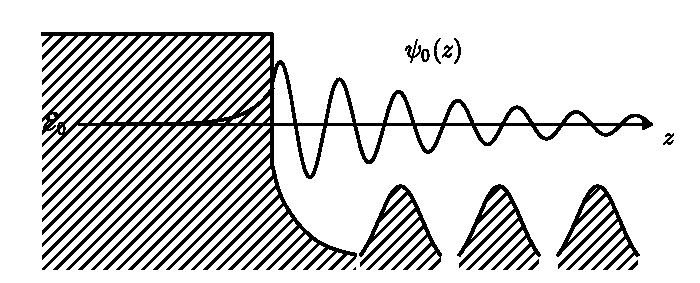
\includegraphics[width=0.72\textwidth]{fig_118.pdf}
\caption*{图 118\quad 表面态。}
\end{figure}

设在某一维模型的一个带隙中，我们已在能量 $\mathcal{E}_{0}$ 处发现了一个定域态 $\psi_{0}(z)$，这个一维模型代表的或许是当我们沿离开表面的 $z$ 方向逐层前进时的平均原子势或赝势。既然晶体在平行于表面的方向上想必仍是周期的，Bloch 定理 (1.58) 对该平面内的平移就必定仍然成立。因此，一维的定域态必定扩展成整整一条\emph{表面态}（surface states）或 \emph{Tamm 态}（Tamm states）的带，其形式为
\begin{equation*}
\psi_{\mathbf{k}}=\psi_{0}(z)\exp i(k_{x}x+k_{y}y), \tag{6.66}
\end{equation*}
其中 $k_{x}$ 和 $k_{y}$ 是在表面平面内量度的波矢的分量。例如在 N.F.E. 情形，我们应预期这条带的行为有如
\begin{equation*}
\mathcal{E}(\mathbf{k})\sim\mathcal{E}_{0}+(\hbar^{2}/2m)(k_{x}^{2}+k_{y}^{2}) \tag{6.67}
\end{equation*}
一直延伸到 $k_{x}$ 与 $k_{y}$ 的倒格子空间中某种二维区边界的类似物为止。

事实上，电子表面态在原理上与 §2.12 中讨论的晶格振动表面模式完全相同。只要对符号作适当的重新标注，我们甚至可以把 (2.138)–(2.145) 的代数演算诠释为在适当边界条件下描写紧束缚模型中的电子表面态。但这类态能够出现的确切能量依赖于模型的细节。即使在一维情形也很显然：势垒的形状及其相对于晶格中最近“原子”的位置，会对 $\psi$ 的局部曲率有举足轻重的影响，从而决定能否实现良好的匹配。在三维情形，情况更加复杂，因为匹配必须在整个表面上进行，而表面绝不会是电子势的一个简单的平面突变。原则上我们可以讨论这类态在给定带隙中出现的条件，但它们对结构细节、化学杂质和空间电荷场的敏感性，阻碍了对能谱及其他性质的定量计算。尽管理论上不可预测，人们还是发现表面态在实际半导体器件的物理中扮演着重要角色：它们可能造成陷阱、复合中心、短路沟道、附加电容以及其他不良效应。这类态在表面催化以及界面上的其他化学现象中也很重要。

真正的表面态只有在功函数势垒之下存在带隙时才能出现。在更高的能量处，与之相应的\emph{倏逝表面波}（evanescent surface waves）在时间上只是准驻定的，类似于共振（参见 §2.12）。这时的典型表面现象便是电子的发射——热发射或光激活发射（见 §8.5）——以及其逆过程：电子从外部射向表面。

高能电子穿过薄膜的衍射已在 §2.6、§3.3 中讨论过。\emph{低能电子衍射}（Low Energy Electron Diffraction, L.E.E.D.）现象则要难作定量解释得多。对于被表面反射回来的电子，晶体动量的法向分量不再是好量子数。衍射峰的基本条件是 (2.79) 的二维类似式，即
\begin{equation*}
\mathbf{k}'_{\parallel}=\mathbf{k}_{\parallel}+\mathbf{g}_{\parallel}, \tag{6.68}
\end{equation*}
其中初始波矢、末态波矢和倒格矢都用它们在平行于表面的平面——即 (6.66) 的 $(x,y)$ 平面——内的投影来表示。反射束的法向分量总可以调节得满足能量守恒条件 $|\mathbf{k}'|^{2}=|\mathbf{k}|^{2}$，因此无论入射束的能量或方向如何，衍射都是允许的。

但要计算衍射强度，我们需要把入射波和反射波同晶体内部 Schrödinger 方程全部解的一个组合相匹配，也就是同固体的\emph{复能带结构}（complex band structure）的所有分支相匹配。不同衍射束的相对强度将依赖于这些内部波函数中相应平面波的相对比例。例如，最强的峰必定出现在入射电子试图以普通 Bloch 态带隙中的能量进入晶体之时——也就是说，接近完整的三维 Bragg--von Laue 衍射条件 (2.79) 处。但在这一区域还可能出现对能量敏感的“共振”效应，此时倏逝表面波可以把电子“导入”不同的衍射束。杂质散射、吸收以及其他非弹性效应，是解释 L.E.E.D. 观测时额外的复杂因素。

\section{电子被杂质散射}

在 §5.2、§5.3 中已经证明，金属中带电杂质的势会受到屏蔽，取 (5.29) 的形式，
\begin{equation*}
\mathcal{U}(\mathbf{r})=\frac{Ze^{2}}{r}\,e^{-\lambda r}, \tag{6.69}
\end{equation*}
其中 $\lambda$ 由 (5.22) 给出。用初等的含时微扰理论容易证明，这个势给出微分散射截面
\begin{equation*}
\sigma(\theta)=\biggl(\frac{2mZe^{2}}{\hbar^{2}}\biggr)^{2}\frac{1}{(K^{2}+\lambda^{2})^{2}}, \tag{6.70}
\end{equation*}
其中 $K=2k_{F}\sin\tfrac{1}{2}\theta$。

对于在半导体中被散射的载流子，类似的结果应当同样成立：此时 $\lambda$ 由 (5.26) 给出，用 $m^{*}$ 代替 $m$，并再乘上一个因子 $1/\epsilon^{2}$ 以顾及介质的介电常数。这不过是等效哈密顿量原理的一次直接应用。

然而，对这些公式不应过分拘泥于字面。它们在求解散射问题时假定了 Born 近似；这对于处于费米能的电子被深势 (6.69) 散射的情形并不很好。更好的做法是使用分波法，
如在式 (5.40) 中那样，并辅以 Friedel 求和规则。再者，我们并不能保证电子波函数真的是简单的平面波——而且势太强，无法恰当地使用等效哈密顿量。最后，散射也不应全部归因于溶质原子与溶剂原子之间的电荷差异；还可能有来自芯势差异的散射——比方说，杂质离子与被它所替代的离子在有效势上有所不同。因此，把 Ag 掺入 Au 中时同样会有散射，尽管二者价数相同，原子体积也几乎完全一样。

由过渡金属杂质引起的散射以 $d$ 共振（§5.5）为主导。由 (3.81) 与 (5.40) 显然可见，散射截面必在 $d$ 相移通过 $\pi/2$ 的共振能量处经过极大值。然而要注意，这一共振可能依赖于杂质的磁极化方向相对于被散射电子自旋取向的关系，如图 95 所示。

在某些情形下，在被散射传导电子的自旋 $\mathbf{s}$ 与杂质处 $d$ 电子的总自旋 $\mathbf{S}$ 之间，还存在一个附加的微弱的\emph{s--d 交换}（s--d-exchange）相互作用。正如 §10.6 将要证明的，这个相互作用的哈密顿量应取如下形式
\begin{equation*}
\mathcal{H}_{s\text{-}d} = -(J/N)\,\mathbf{S}\cdot\mathbf{s}, \tag{6.71}
\end{equation*}
其中“交换”参量 $J$ 通常为负。这具有重要的物理后果，因为入射电子的自旋在被散射时可能被“翻转”。

在半导体中，还可能有来自中性杂质的散射——例如，一个电子已落入施主杂质能级，或者一个空穴驻留在受主能级上（§§6.4、6.7）。这时的散射计算是一个相当可观的问题，等同于计算慢电子被中性氢原子散射的问题。

\section{绝热原理}

现在我们要考虑传导电子与格波之间的相互作用。这乍看是一个极其复杂的动力学问题——直到我们发现它可以拿初等微扰论来处理。这样做的依据是 Born--Oppenheimer 定理，下面我们就来推导它。

让我们写下离子与电子整个系统的哈密顿算符。如同第 2 章那样，令 $\mathbf{u}_l$ 代表第 $l$ 个离子相对于第 $l$ 个格点的位置（为简单起见，我们假定每个晶胞只含一个原子）；令 $\mathbf{r}_i$ 代表第 $i$ 个电子的位置。总哈密顿量为
\begin{equation*}
\mathcal{H} = -\sum_{l}\frac{\hbar^{2}}{2M}\frac{\partial^{2}}{\partial\mathbf{u}_{l}^{2}} - \sum_{i}\frac{\hbar^{2}}{2m}\frac{\partial^{2}}{\partial\mathbf{r}_{i}^{2}} + \sum_{i<j}\frac{e^{2}}{|\mathbf{r}_{i}-\mathbf{r}_{j}|} + \mathcal{V}(\mathbf{u},\mathbf{r}) + G(\mathbf{u}). \tag{6.72}
\end{equation*}
头两项是离子和电子的动能算符。下一项是电子间相互作用。再下一项是电子在离子（处于其位移后的位置）场中的势能。最后，$G(\mathbf{u})$ 代表离子之间任何直接作用的势能。

让我们试着取如下的函数作为这个哈密顿量的一个本征函数：
\begin{equation*}
\Psi = \psi(\mathbf{u},\mathbf{r})\,\Phi(\mathbf{u}), \tag{6.73}
\end{equation*}
其中我们让 $\psi$ 满足电子在静态晶格——被冻结、第 $l$ 个离子位于 $\mathbf{u}_l$ 处——中的 Schr\"odinger 方程
\begin{equation*}
\biggl\{\sum_{i}-\frac{\hbar^{2}}{2m}\frac{\partial^{2}}{\partial\mathbf{r}_{i}^{2}} + \sum_{ij}\frac{e^{2}}{|\mathbf{r}_{i}-\mathbf{r}_{j}|} + \mathcal{V}(\mathbf{u},\mathbf{r})\biggr\}\,\psi(\mathbf{u},\mathbf{r}) = \mathcal{E}_{e}(\mathbf{u})\,\psi(\mathbf{u},\mathbf{r}). \tag{6.74}
\end{equation*}
这可以——事实上也必须——是一个多电子波函数；我们仍然假定能够求出它的本征值 $\mathcal{E}_{e}(\mathbf{u})$，例如把它们当作一组准粒子能级。但这些本征值将是 $\mathbf{u}_l$ 的函数；电子气的能量将依赖于离子的位置。

现在把算符 $\mathcal{H}$ 作用到这个波函数上：
\begin{align*}
\mathcal{H}\Psi &= -\sum_{l}\frac{\hbar^{2}}{2M}\frac{\partial^{2}}{\partial\mathbf{u}_{l}^{2}}\,\Psi + \mathcal{E}_{e}(\mathbf{u})\Psi + G(\mathbf{u})\Psi \\
&= \psi(\mathbf{u},\mathbf{r})\biggl\{-\sum_{l}\frac{\hbar^{2}}{2M}\frac{\partial^{2}}{\partial\mathbf{u}_{l}^{2}} + \mathcal{E}_{e}(\mathbf{u}) + G(\mathbf{u})\biggr\}\Phi(\mathbf{u}) \\
&\quad -\sum_{l}\frac{\hbar^{2}}{2M}\biggl\{2\frac{\partial\Phi}{\partial\mathbf{u}_{l}}\cdot\frac{\partial\psi}{\partial\mathbf{u}_{l}} + \Phi\frac{\partial^{2}\psi}{\partial\mathbf{u}_{l}^{2}}\biggr\}. \tag{6.75}
\end{align*}
倘若此表达式中的第二行可以忽略，我们便能令 $\Phi(\mathbf{u})$ 满足一个 Schr\"odinger 型方程，从而求解完整的本征值问题 $\mathcal{H}\Psi = \mathcal{E}\Psi$：
\begin{equation*}
\biggl\{-\sum_{l}\frac{\hbar^{2}}{2M}\frac{\partial^{2}}{\partial\mathbf{u}_{l}^{2}} + \mathcal{E}_{e}(\mathbf{u}) + G(\mathbf{u})\biggr\}\,\Phi(\mathbf{u}) = \mathcal{E}\,\Phi(\mathbf{u}). \tag{6.76}
\end{equation*}
这就是说，我们必须在离子之间的直接相互作用之外，再加上 $\mathcal{E}_{e}(\mathbf{u})$ 一项，它是电子系统的总能量作为离子位置的函数。这就是电子对晶格能量的\emph{绝热}（adiabatic）贡献。它是电子为了跟随晶格运动而不得不付出的能量改变。原则上，这一项将依赖于电子组态的细节，例如依赖于在金属温度下被激发的准粒子的数目——但实际上它对这类差别非常不敏感，通常可以假定电子处于基态来进行计算。

还有必要证明 (6.75) 中的非绝热项可以忽略。容易证明，它们对系统处于态 $\Psi$ 时的能量期望值几乎没有贡献。第一个这样的项为零：它将给出如下形式的积分
\begin{align*}
\int\psi^{*}\frac{\partial\psi}{\partial\mathbf{u}_{l}}\,\mathbf{dr} &= \frac{1}{2}\frac{\partial}{\partial\mathbf{u}_{l}}\int\psi^{*}\psi\,\mathbf{dr} \\
&= \frac{1}{2}\frac{\partial n_{e}}{\partial\mathbf{u}_{l}}, \tag{6.77}
\end{align*}
其中 $n_{e}$ 是电子的总数。第二项之所以小，是因为往最坏里说，电子也不过是被紧紧束缚在各自的离子上
\begin{equation*}
\psi(\mathbf{u}_{l},\mathbf{r}_{i}) = \psi(\mathbf{r}_{i}-\mathbf{u}_{l}), \tag{6.78}
\end{equation*}
这会给出如下形式的贡献
\begin{align*}
-\int\psi^{*}\frac{\hbar^{2}}{2M}\frac{\partial^{2}\psi}{\partial\mathbf{u}_{l}^{2}}\,\mathbf{dr} &= -\int\psi^{*}\frac{\hbar^{2}}{2M}\frac{\partial^{2}\psi}{\partial\mathbf{r}_{i}^{2}}\,\mathbf{dr} \\
&= -\frac{m}{M}\int\psi^{*}\frac{\hbar^{2}}{2m}\frac{\partial^{2}\psi}{\partial\mathbf{r}_{i}^{2}}\,\mathbf{dr}. \tag{6.79}
\end{align*}
这不过是电子动能的 $m/M$ 倍——与寻常的热能相比可以忽略不计，因为 $m/M$ 的量级为 $10^{-4}$ 或 $10^{-5}$。

我们刚才只是非常抽象地勾画了这一论证，它没有考虑非对角的非绝热项。特别是其中的第一项，含有 $\partial\psi/\partial\mathbf{u}_{l}$，当离子运动时能够在电子态之间引起跃迁。这恰恰就是\emph{电子--声子相互作用}（electron--phonon interaction），我们将在 §6.13 中讨论它。我们在 (6.77) 中所证明的只不过是它的对角元为零。若计入涉及此项非对角元的二阶微扰，我们将得到对晶格能量的贡献。

绝热原理之所以重要，是因为它使我们得以把离子的运动与电子的运动分开，而在电子与声子之间只留下一个残余的相互作用。它为我们证实了一个直观的观念：电子气的能量是固体总弹性能的一个重要组成部分——正如在讨论金属内聚性（§4.3）时所假定的那样。计入这个能量项之后，我们就可以把电子和格波当作近乎独立的实体来处理。

\section{声速的重整化}

绝热原理诱使我们作如下简单的论证。假设我们计算一个裸离子晶格的振动谱。那么加入电子会有什么影响？

碰巧，我们可以不费任何气力就得出一个结果。由点电荷组成的晶格的长波纵振动会引起体积变化和极化场，它们可以宏观地计算出来，一如 (5.60)--(5.62)。设正离子的密度为每单位体积 $N$ 个、质量为 $M$、电荷为 $Ze$，其位移的运动方程为
\begin{equation*}
M\ddot{\mathbf{x}} = -4\pi NZ^{2}e^{2}\mathbf{x}. \tag{6.80}
\end{equation*}
这就是说，对于波矢为 $\mathbf{q}$ 的纵波，其频率就是离子的等离体频率
\begin{equation*}
\Omega_{p} = \biggl(\frac{4\pi NZ^{2}e^{2}}{M}\biggr)^{\frac{1}{2}}, \tag{6.81}
\end{equation*}
而且几乎不依赖于 $q$。

现在假设我们把电子气倾注进去。如第 5 章所示，这会修正来自其他源的一切有效静电场。例如，波矢为 $\mathbf{q}$、频率为 $\omega$ 的外加场要除以在 (5.16) 中定义的介电函数 $\epsilon(\mathbf{q},\omega)$。这应当同样适用于源于离子等离体极化的力；(6.80) 的右端应当除以 $\epsilon(\mathbf{q},\omega)$，其中 $\mathbf{q}$ 是所考虑的振动的波矢，$\omega$ 是它的实际频率。这意味着观测到的频率将是
\begin{equation*}
\nu_{\mathbf{q}}^{2} = \frac{\Omega_{p}^{2}}{\epsilon(\mathbf{q},\nu_{\mathbf{q}})}. \tag{6.82}
\end{equation*}
实际上 $\nu_{\mathbf{q}}$ 很小，在 $\epsilon$ 中可以忽略（也就是说，离子等离体振动的频率与一切电子过程相比都很低）。对 $\epsilon(\mathbf{q},0)$ 采用近似 (5.21)，我们得到
\begin{equation*}
\nu_{\mathbf{q}}^{2} \approx \frac{4\pi NZ^{2}e^{2}}{M}\,\frac{q^{2}}{q^{2}+4\pi e^{2}\mathcal{N}(\mathcal{E}_{F})}, \tag{6.83}
\end{equation*}
亦即
\begin{equation*}
\nu_{\mathbf{q}} \rightarrow q\biggl(\frac{NZ^{2}}{M\mathcal{N}(\mathcal{E}_{F})}\biggr)^{\frac{1}{2}}. \tag{6.84}
\end{equation*}
换句话说，纵声学模的速度趋于一个常数；对于密度为 $NZ$ 的自由电子气，它就是简单地
\begin{equation*}
s = \biggl(\frac{mZ}{3M}\biggr)^{\frac{1}{2}}v_{F}, \tag{6.85}
\end{equation*}
其中 $v_{F}$ 照例是电子的费米速度。对大多数金属的声速而言，这个估计并不坏，对碱金属尤其好用。公式 (6.82) 表明 Kohn 效应（§5.4）是如何产生的。群速是 $\nu_{\mathbf{q}}$ 对 $q$ 的导数——而 $\epsilon(\mathbf{q},0)$ 的导数在 $q = 2k_{F}$ 处含有对数奇异性。

要对金属的晶格动力学作更系统的处理——对一切偏振方向、一切波长都成立——我们应当按如下步骤进行：(i) 计算完整晶体的电子能带结构；(ii) 计算同一晶体在离子按波矢为 $\mathbf{q}$ 的声子图样（如 (2.49) 那样）发生位移时的能带结构；(iii) 把这两个结构的总能量之差当作这种位移图样中“势能”的改变（如 (2.2) 那样），从而算出该模的频率 $\omega_{\mathbf{q}}$。

这个程序看上去令人生畏，因为绝热原理只有在每个结构都自洽地算出时才成立。但假设我们处理的是横声子模，其中局地原子体积保持不变。晶体内聚能的大部分（参看 §4.3）不发生变化，于是我们可以只集中于来自费米面畸变的小贡献——这样的畸变可以描述成电子被位移了的离子散射所产生的微扰（参看 §§2.7、6.13）。对于简单的 N.F.E. 金属，§5.3 的屏蔽赝势方案恰好精确地、完全自洽地描述了这类位移的效应。于是我们发现频率 $\omega_{\mathbf{q}}$ 与屏蔽离子赝势的各个 Fourier 分量 $w_{s}(\mathbf{q}+\mathbf{g})$ 之间有一个关系式。

这个关系已被颇为成功地用于解释用中子衍射（§2.8）在金属横向晶格谱中观测到的复杂色散曲线。我们甚至可以回到实空间表示，证明金属的动力学行为就好像“中性赝原子”（neutral pseudo-atoms）之间存在两两成对的弹性力——这种力也可以解释成裸金属离子的“赝电荷”云之间的屏蔽静电相互作用。但这个图像用于长波纵模时却会引人误入歧途，因为在那里体积效应占主导地位；对于过渡金属和共价键合的半导体（§4.2），它也完全不适用。

\section{电子–声子相互作用}

处理这个问题的最简单方式，是假定金属中的传导电子被晶格振动非弹性地衍射，其方式与我们为 X 射线、中子或快电子的非弹性衍射所假定的完全相同。这个处理乍一看实在太过天真，但可以求助于 §6.11 的绝热原理来为它辩护。我们径直接过 §§2.7、2.8 的全部理论。在 (2.86) 与 (2.97) 中我们得到过如下公式：从态 $\mathbf{k}$ 到态 $\mathbf{k}'$ 的跃迁矩阵元可以写成
\begin{equation*}
\mathcal{M}_{\mathbf{k}\mathbf{k}'} = i\mathcal{V}_{a}(\mathbf{K})\cdot(\mathbf{K}\cdot\mathbf{U}_{\mathbf{q}}), \tag{6.86}
\end{equation*}
其中 $\mathbf{K} = \mathbf{k}' - \mathbf{k}$；$\mathbf{q} = \mathbf{K}$ 或 $\mathbf{q} = \mathbf{K} - \mathbf{g}$，视我们遇到的是 N 过程还是 U 过程而定；$\mathbf{U}_{\mathbf{q}}$ 是波矢为 $\mathbf{q}$ 的晶格振动的矢量振幅；而 $\mathcal{V}_{a}(\mathbf{K})$ 是单个原子或离子的势对这个跃迁的矩阵元。

我们可以把它非常简单地表述如下。取 $\mathcal{M}_{\mathbf{k}\mathbf{k}'}$ 的模平方，再用常规微扰论算出一个散射概率。于是晶格中每个原子的行为就如同它具有一个平均的有效微分散射截面
\begin{equation*}
\overline{\sigma}(\mathbf{K}) = \sigma_{a}(\mathbf{K})\,N\,|\mathbf{K}\cdot\mathbf{U}_{\mathbf{q}}|^{2}, \tag{6.87}
\end{equation*}
其中 $\sigma_{a}(\mathbf{K})$ 是\emph{孤立的}（isolated）原子散射过矢量 $\mathbf{K}$ 的微分截面。

这个公式十分透明。它仿佛是说每个原子都能独立地散射电子——但散射量的多少依赖于它在晶格中与相邻原子相对位移的大小。因子 $|\mathbf{K}\cdot\mathbf{U}_{\mathbf{q}}|^{2}$ 对所有 $\mathbf{q}$ 的平均出现在 §2.9 讨论的 Debye--Waller 因子的理论之中；如 (2.107) 与 (2.118) 所示，它正是离子偏离其格点的均方位移，表示为晶格间距的分数。但当我们细致考察每一个过程——也就是说，当我们选定一个特定的 $\mathbf{K}$ 值时——就必须考虑来自具有确定波矢的一组晶格位移的散射；此时相邻离子位移之间的关联就变得重要起来，长波模引起的散射遂被削弱。

参看 (2.86) 与 (2.103)，我们可以把这一点看得更加清楚。因子 $N|\mathbf{K}\cdot\mathbf{U}_{\mathbf{q}}|^{2}$ 是结构因子平方的一个近似，而结构因子正比于 $S(\mathbf{K})$，即原子位置的对关联函数（pair correlation function）的 Fourier 变换；亦即
\begin{equation*}
\overline{\sigma}(\mathbf{K}) = \sigma_{a}(\mathbf{K})\,S(\mathbf{K}). \tag{6.88}
\end{equation*}
这个结果对液体和对固体同样成立；传导电子的散射依赖于液体中原子的径向分布函数。

等我们讨论电阻率等问题时，还要进一步考虑这个结构因子，并分析来自各个晶格频率的贡献。我们还需要计入电子被散射时的能量变化，一如 (2.101)。眼下我们只指出：绝热原理使我们得以证明 (6.87)，因为它允许我们假定晶格冻结在任一构型上，然后再计算电子在这个稍稍非周期的排布中的散射。离子运动的唯一动力学效应，就是我们方才提到的那个能量变化。

电子--声子相互作用的问题就这样主要归结为计算 $\sigma_{a}(\mathbf{K})$。假如原子只是一个被整体携带着走的浅势 $\mathcal{V}(\mathbf{r})$，那么由初等波力学，在 Born 近似下我们应当有
\begin{equation*}
\frac{\partial\sigma_{a}}{\partial\Omega} = \biggl(\frac{m}{2\pi\hbar^{2}N}\biggr)^{2}\,|\mathcal{V}_{a}(\mathbf{K})|^{2} \tag{6.89}
\end{equation*}
作为每单位立体角 $\Omega$ 的微分散射。在这个公式中
\begin{equation*}
\mathcal{V}_{a}(\mathbf{K}) = N\int\mathcal{V}_{a}(\mathbf{r})\,e^{-i\mathbf{K}\cdot\mathbf{r}}\,\mathbf{dr}; \tag{6.90}
\end{equation*}
它是离子势的 Fourier 变换，按晶体的一个晶胞归一化。

但是正如 §3.9 中所见，原子或离子的真实势对散射截面的 Born 近似来说太深了。分波公式 (3.78)，或某种类似的散射振幅精确公式，要合适得多。特别是，我们可以采用 §§3.6、3.9 的赝势形式体系，在与能带结构计算相同的框架内计算电子--声子相互作用。

这就提示我们，(6.89) 中 $\mathcal{V}_{a}$ 的 Fourier 分量应当换成原子赝势的相应分量。
但移动一个离子所引起的势的改变，必须把电子气电荷分布的移动所产生的任何效应都包括进来。如 §5.3 所见，这可以近似地加以照顾：把裸离子势的 Fourier 分量除以介电函数。

长话短说，正确的做法是使我们关于电子--声子相互作用的整个讨论从叠加的\emph{赝原子}（pseudo-atom）势 (5.35) 出发，而不是从叠加的“原子”势 (2.83) 出发。代替 (6.89)，我们得到
\begin{equation*}
\frac{\partial\sigma_{a}}{\partial\Omega} = \biggl(\frac{m}{2\pi\hbar^{2}N}\biggr)^{2}\,|w_{s}(K)|^{2}, \tag{6.91}
\end{equation*}
其中 $w_{s}(K)$ 是某个中性赝原子“势”的 Fourier 变换。这个公式在散射微扰级数的所有阶次上并不精确，而且在 $K$ 大时相当不确定，因为线性屏蔽在原子芯区内并不适用；但对于简单的 N.F.E. 金属，它是一个良好的自洽近似。

$w_{s}(K)$ 的行为对所有简单金属而言大体相同。如 §5.3 所见，\emph{裸}（bare）离子的赝势 $w_{b}(r)$ 包含价电荷 $Ze$ 的长程 Coulomb 场。因此，作 Fourier 变换后（参看 (5.31)），它必定表现如下
\begin{equation*}
w_{b}(K) \approx -\frac{4\pi ZNe^{2}}{K^{2}} + \mathcal{V}'(K) \tag{6.92}
\end{equation*}
其中当 $\mathbf{K} \rightarrow 0$ 时 $\mathcal{V}'(\mathbf{K})$ 保持有限，无论离子芯内部 $\mathcal{V}(\mathbf{r})$ 的形式如何。

(6.92) 中的奇异性当然在 $\mathbf{K} = \mathbf{0}$ 处被 $\epsilon(\mathbf{K})$ 的奇异性所抵消，一如 (5.32)。把这些不同的结果合在一起，我们可以写出
\begin{align*}
w_{s}(K) = \frac{w_{b}(K)}{\epsilon(K)} &\approx \frac{-4\pi ZNe^{2}/K^{2} + \mathcal{V}'(\mathbf{K})}{1 + 4\pi e^{2}\mathcal{N}(\mathcal{E}_{F})/K^{2}} \\
&\approx \frac{-\frac{2}{3}\mathcal{E}_{F} + (K^{2}/\lambda^{2})\,\mathcal{V}'(\mathbf{K})}{1 + (K^{2}/\lambda^{2})}, \tag{6.93}
\end{align*}
其中屏蔽参量 $\lambda$ 来自 (5.22)，或者更确切地说，来自 (5.21) 与 (5.36)。本质上，这就是 Bardeen 在 1937 年为碱金属中电子--声子相互作用的矩阵元导出的公式。我们现在看到，这个赝原子形状因子（图 119）在简单的
N.F.E. 金属的理论中占据核心地位。知道了 $w_{s}(K)$，我们原则上就可以计算能带结构（§3.9）、晶格谱（§6.12）、晶相与液相的电输运性质（§7.5），甚至超导转变温度（§11.1）。遗憾的是，(6.93) 中的芯贡献 $\mathcal{V}'(\mathbf{K})$ 既不是“局域的”（§3.6），也没有唯一的定义，因此这些性质之间的关联并不如我们所期望的那样完美。生活很少那么简单！

\begin{figure}[H]
\centering
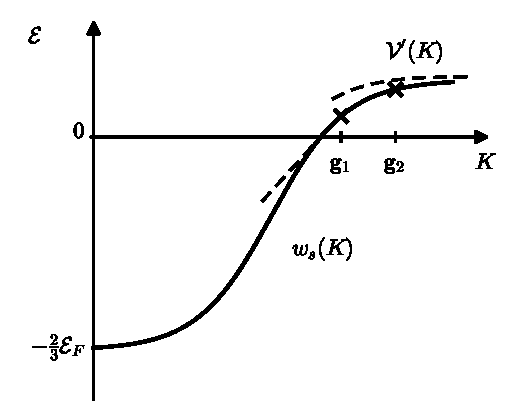
\includegraphics[width=0.72\textwidth]{fig_119.pdf}
\caption*{图 119\quad 赝原子形状因子。能带结构只依赖于它在倒格矢 $\mathbf{g}_1$、$\mathbf{g}_2$ 等处的取值。}
\end{figure}

\begin{figure}[H]
\centering
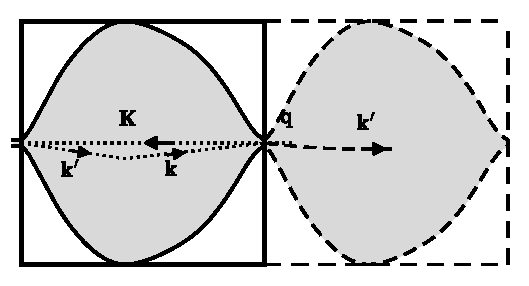
\includegraphics[width=0.72\textwidth]{fig_120.pdf}
\caption*{图 120\quad 在重复区图式中，U 过程可以化为 N 过程。}
\end{figure}

在这番讨论中有一点需要当心。假设我们要求两个电子态 $\mathbf{k}$ 与 $\mathbf{k}'$ 之间的电子--声子相互作用，而这两个态相距几乎恰好一个倒格矢。这时若用诸如 (6.89) 那样的自由电子公式来计算微分散射截面，就肯定错了。这两个态看似相差一个很大的波矢，其实在重复区图式上看彼此相当接近。由于二者都贴近某个区边界，正如 §§3.2、3.3 中指出的，每一个都是平面波的复杂混合。
就可以发现（出于自洽性的要求也必然如此）：当把 $\mathcal{V}_{a}(\mathbf{K})$ 作为在经过正确混合的波函数之间取的矩阵元来计算时，它的值在 $\mathbf{K} \rightarrow \mathbf{g}$ 时趋于零。

我们可以换一种说法。一个在单一简约区内标记时看似倒逆过程的跃迁，在重复区图式中可以显得像正常过程——而且此时矩阵元正比于 $\mathbf{q}\cdot\mathbf{U}_{\mathbf{q}}$，当声子波矢 $\mathbf{q}$ 趋于零时它也趋于零。

\section{形变势}

在半导体中，波函数十分复杂，方便的办法是采用一种唯象理论，把晶体当作连续的弹性介质来处理。这时晶格振动可以描述成弹性应变的波，例如
\begin{equation*}
\mathsf{W}_{ij}(\mathbf{r}) = \mathsf{W}_{ij}^{0}\,e^{i\mathbf{q}\cdot\mathbf{r}} \tag{6.94}
\end{equation*}
给出 $\mathbf{r}$ 处应变张量的笛卡尔分量。于是我们论证：局域应变使载流子的能量改变如下的数量
\begin{equation*}
\delta\mathcal{E}(\mathbf{r}) = \sum_{ij}\mathcal{E}_{ij}\,\mathsf{W}_{ij}(\mathbf{r}), \tag{6.95}
\end{equation*}
其中 $\mathcal{E}_{ij}$ 是\emph{形变势}（deformation potential）张量。

我们可以容易地算出一个电子散射的矩阵元。譬如说，如 (2.84) 中那样，
\begin{align*}
\mathcal{M}_{\mathbf{k}\mathbf{k}'} &= \int e^{-i\mathbf{k}'\cdot\mathbf{r}}\,\delta\mathcal{E}(\mathbf{r})\,e^{i\mathbf{k}\cdot\mathbf{r}}\,\mathbf{dr} \\
&= \bigl(\sum_{ij}\mathsf{W}_{ij}^{0}\,\mathcal{E}_{ij}\bigr)\delta_{\mathbf{k}-\mathbf{k}'+\mathbf{q}}, \tag{6.96}
\end{align*}
这是在单位体积的晶体中。

这种散射守恒晶体动量；这很自然，因为我们已经把晶格抹平了。散射概率正比于 $|\mathsf{W}^{0}|^{2}$，它与更精确的理论中 (6.88) 的结构因子属于同一类量。为了求出系数 $\mathcal{E}_{ij}$，我们可以设想让整个固体经受均匀应变 $\mathsf{W}^{0}$，并测量能隙宽度的改变。

对于金属，$\mathcal{E}_{ij}$ 的膨胀分量很容易确定。论证本质上就是 §5.2 中所用的那一套。一个变化的体膨胀 $\Delta(\mathbf{r})$ 使 $\mathbf{r}$ 附近的电子密度从 $n_{0}$ 变为 $n_{0}(1-\Delta)$。这会使费米能级改变
\begin{equation*}
\delta\zeta(\mathbf{r}) = \frac{n_{0}\Delta(\mathbf{r})}{\mathcal{N}(\mathcal{E}_{F})} = \frac{2}{3}\mathcal{E}_{F}\Delta(\mathbf{r}) \tag{6.97}
\end{equation*}
——在自由电子气中。对于密度的长波振荡，我们可以让少数电子从较稠密的区域回流出来，从而使费米能级恢复均匀。这个对局域电中性的小偏离产生一个电场，其势恰好使费米能级在整个晶体中恢复处处相同。这个场必定是 $-\delta\zeta(\mathbf{r})$，我们把它等同于 $\delta\mathcal{E}(\mathbf{r})$；也就是说，形变势张量的迹必为
\begin{equation*}
\sum_{i}\mathcal{E}_{ii} = -\frac{2}{3}\mathcal{E}_{F}. \tag{6.98}
\end{equation*}

\begin{figure}[H]
\centering
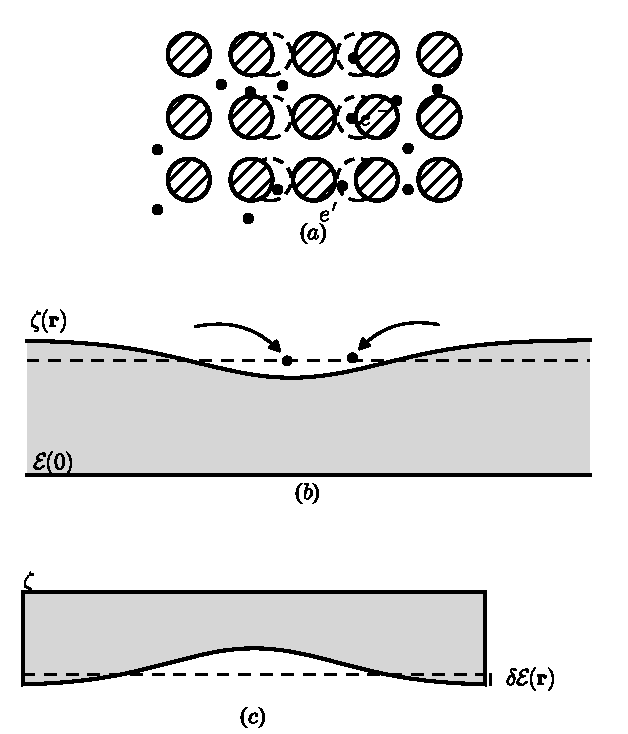
\includegraphics[width=0.72\textwidth]{fig_121.pdf}
\caption*{图 121\quad (a) 晶格中的密度波使电子密度发生变化。(b) 费米能级被升高或降低。(c) 电子回流以保持费米能级恒定，从而产生形变势。}
\end{figure}

这是对 (6.93) 中 $w_{s}(K)$ 在 $K \rightarrow 0$ 时的极限值的一个严格推导；它表明赝原子形状因子的这个特征是完全自洽的，而且对微扰论的所有阶次都精确。任何想在发生了形变的晶体中使用 muffin-tin 势（§3.7）的做法，也都必须把这个效应作为 muffin-tin 零点的改变考虑进去。

 % 本文件由 scripts/assemble.py 自动装配，勿手改（改 parts/ 后重跑）
% 第7章 输运性质

% 第7章 Transport Properties

\chapter{输运性质}

\epigraphbook{没有谁喊“一、二、三，预备——跑！”，\\ 它们喜欢什么时候开始跑就什么时候开始跑，喜欢什么时候停就什么时候停，\\ 所以很难说清这场比赛究竟什么时候才算结束。}{LEWIS CARROLL}

\section{Boltzmann 方程}

金属或半导体中的载流子会受到外场的影响，也会受到温度梯度的影响。它们还会遭受来自杂质、格波等的散射。这些效应必须相互达到平衡——我们必须考虑这样的情形：电子被电场加速，却又通过散射失去其多余的能量和动量。在本章中，我们将考虑“普通的”输运性质，也就是加上恒定场时所观察到的那些性质。

一般说来，处理这个问题远为最简单的途径，是建立输运方程（transport equation）即 Boltzmann 方程。我们研究一个量 $f_{\mathbf{k}}(\mathbf{r})$，它表示在空间中点 $\mathbf{r}$ 附近处于态 $\mathbf{k}$ 的载流子的局域浓度。严格地说，这个量只能借助细粒度分布、系综平均、密度矩阵等来定义。关于这一点已有相当多的文献——但它更多属于量子统计力学的形式理论，而不是固体理论。

现在考虑 $f_{\mathbf{k}}(\mathbf{r})$ 如何随时间变化。有三类效应：

（i）载流子会流入和流出区域 $\mathbf{r}$。设 $\mathbf{v}_{\mathbf{k}}$ 是态 $\mathbf{k}$ 中载流子的速度。那么，在时间间隔 $t$ 内，这个态中的载流子移动一段距离 $t\mathbf{v}_{\mathbf{k}}$。于是，根据 Liouville 关于相空间中所占据体积不变的定理，$t$ 时刻位于 $\mathbf{r}$ 附近的载流子数目，等于 $0$ 时刻位于 $\mathbf{r}-t\mathbf{v}_{\mathbf{k}}$ 附近的数目：
\begin{equation*}
f_{\mathbf{k}}(\mathbf{r},t)=f_{\mathbf{k}}(\mathbf{r}-t\mathbf{v}_{\mathbf{k}},0).\tag{7.1}
\end{equation*}
这意味着，由于扩散引起的分布的变化率为
\begin{equation*}
\left.\frac{\partial f_{\mathbf{k}}}{\partial t}\right]_{\text{diff.}}
=-\mathbf{v}_{\mathbf{k}}\cdot\frac{\partial f_{\mathbf{k}}}{\partial \mathbf{r}}
=-\mathbf{v}_{\mathbf{k}}\cdot\nabla f_{\mathbf{k}}.\tag{7.2}
\end{equation*}

（ii）外场会改变每个载流子的 $\mathbf{k}$ 矢量，其变化率为式 (6.40)，即
\begin{equation*}
\dot{\mathbf{k}}=\frac{e}{\hbar}\left(\mathbf{E}+\frac{1}{c}\mathbf{v}_{\mathbf{k}}\wedge\mathbf{H}\right).\tag{7.3}
\end{equation*}
我们可以把它看作载流子在 $\mathbf{k}$ 空间中的速度，于是，通过与式 (7.1) 类比，
\begin{equation*}
f_{\mathbf{k}}(\mathbf{r},t)=f_{\mathbf{k}-\dot{\mathbf{k}}t}(\mathbf{r},0);\tag{7.4}
\end{equation*}
也就是说，由于场（\emph{fields}）的作用，分布以下列速率变化：
\begin{align*}
\left.\frac{\partial f_{\mathbf{k}}}{\partial t}\right]_{\text{field}}
&=-\dot{\mathbf{k}}\cdot\frac{\partial f_{\mathbf{k}}}{\partial\mathbf{k}}\\
&=-\frac{e}{\hbar}\left(\mathbf{E}+\frac{1}{c}\mathbf{v}_{\mathbf{k}}\wedge\mathbf{H}\right)\cdot\frac{\partial f_{\mathbf{k}}}{\partial\mathbf{k}}\tag{7.5}
\end{align*}
（其中我们把 $\partial/\partial\mathbf{k}$ 写作 $\mathbf{k}$ 空间中的梯度——即算符 $\nabla_{\mathbf{k}}$）。

（iii）散射的效应更为复杂。但我们在此主要限于弹性散射。它使 $f_{\mathbf{k}}$ 获得一个变化率
\begin{equation*}
\left.\frac{\partial f_{\mathbf{k}}}{\partial t}\right]_{\text{scatt.}}
=\int\{f_{\mathbf{k}'}(1-f_{\mathbf{k}})-f_{\mathbf{k}}(1-f_{\mathbf{k}'})\}\,Q(\mathbf{k},\mathbf{k}')\,\mathrm{d}\mathbf{k}'.\tag{7.6}
\end{equation*}
由 $\mathbf{k}$ 散射到 $\mathbf{k}'$ 的过程使 $f_{\mathbf{k}}$ 减小。这一过程的概率既取决于 $f_{\mathbf{k}}$，即态 $\mathbf{k}$ 中载流子的数目，也取决于 $(1-f_{\mathbf{k}'})$，即末态中可供占用的空位数目。同时还存在逆过程，即从 $\mathbf{k}'$ 进入 $\mathbf{k}$ 的过程，它使 $f_{\mathbf{k}}$ 增大，其权重为 $f_{\mathbf{k}'}(1-f_{\mathbf{k}})$。我们对所有其他可能的态 $\mathbf{k}'$ 求和。不过，对于每一对 $\mathbf{k}$ 和 $\mathbf{k}'$，都存在一个基本跃迁概率 $Q(\mathbf{k},\mathbf{k}')$，它量度跃迁速率——比如说，在已知 $\mathbf{k}$ 被占据而 $\mathbf{k}'$ 为空的情形下。\emph{微观可逆性}（microscopic reversibility）原理告诉我们，同一个函数也给出从 $\mathbf{k}'$ 到 $\mathbf{k}$ 的跃迁速率，所以它是被积函数中的一个公共因子。

Boltzmann 方程说：在任一点、对任意的 $\mathbf{k}$ 值，$f_{\mathbf{k}}(\mathbf{r})$ 的净变化率为零，即
\begin{equation*}
\left.\frac{\partial f_{\mathbf{k}}}{\partial t}\right]_{\text{scatt.}}
+\left.\frac{\partial f_{\mathbf{k}}}{\partial t}\right]_{\text{field}}
+\left.\frac{\partial f_{\mathbf{k}}}{\partial t}\right]_{\text{diff.}}=0.\tag{7.7}
\end{equation*}

注意，这是一个\emph{定常态}（steady state），而不是\emph{平衡态}（equilibrium state）；平衡态我们记作 $f_{\mathbf{k}}^{0}$，它在没有场和温度梯度时成立。如果外场本身随时间变化，那么这三项之和必须等于 $f_{\mathbf{k}}$ 在此力作用下随时间的变化（见 §8.6）。

但我们假定，定态分布不会偏离平衡太远。我们写出
\begin{equation*}
g_{\mathbf{k}}=f_{\mathbf{k}}-f_{\mathbf{k}}^{0},\tag{7.8}
\end{equation*}
其中，如 §4.5 中那样，
\begin{equation*}
f_{\mathbf{k}}^{0}=\frac{1}{\exp\{(\mathcal{E}_{\mathbf{k}}-\zeta)/kT\}+1}=f^{0}(\mathcal{E}_{\mathbf{k}}).\tag{7.9}
\end{equation*}

这里我们必须稍稍小心一点：当温度逐点各不相同时，$f_{\mathbf{k}}^{0}$ 该如何定义？我们假定每一点都有一个明确确定的温度 $T(\mathbf{r})$，并写出
\begin{equation*}
g_{\mathbf{k}}(\mathbf{r})=f_{\mathbf{k}}(\mathbf{r})-f_{\mathbf{k}}^{0}\{T(\mathbf{r})\}.\tag{7.10}
\end{equation*}
如果难以确定 $T(\mathbf{r})$ 应当取什么，我们可以坚持要求最终解满足某个附加条件，例如
\begin{equation*}
\int g_{\mathbf{k}}(\mathbf{r})\,\mathrm{d}\mathbf{k}=0.\tag{7.11}
\end{equation*}

把式 (7.8) 代入式 (7.7)，并利用式 (7.2) 和式 (7.5)，Boltzmann 方程变为
\begin{equation*}
-\mathbf{v}_{\mathbf{k}}\cdot\frac{\partial f_{\mathbf{k}}}{\partial\mathbf{r}}
-\frac{e}{\hbar}\left(\mathbf{E}+\frac{1}{c}\mathbf{v}_{\mathbf{k}}\wedge\mathbf{H}\right)\cdot\frac{\partial f_{\mathbf{k}}}{\partial\mathbf{k}}
=-\left.\frac{\partial f_{\mathbf{k}}}{\partial t}\right]_{\text{scatt.}},\tag{7.12}
\end{equation*}
亦即
\begin{align*}
-\mathbf{v}_{\mathbf{k}}\cdot\frac{\partial f_{\mathbf{k}}^{0}}{\partial T}\nabla T
-\frac{e}{\hbar}\left(\mathbf{E}+\frac{1}{c}\mathbf{v}_{\mathbf{k}}\wedge\mathbf{H}\right)\cdot\frac{\partial f_{\mathbf{k}}^{0}}{\partial\mathbf{k}}\\
=-\left.\frac{\partial f_{\mathbf{k}}}{\partial t}\right]_{\text{scatt.}}
+\mathbf{v}_{\mathbf{k}}\cdot\frac{\partial g_{\mathbf{k}}}{\partial\mathbf{r}}
+\frac{e}{\hbar}\left(\mathbf{E}+\frac{1}{c}\mathbf{v}_{\mathbf{k}}\wedge\mathbf{H}\right)\cdot\frac{\partial g_{\mathbf{k}}}{\partial\mathbf{k}}.\tag{7.13}
\end{align*}

借助式 (7.9) 以及运动学关系式 (6.2)，我们可以把它写成
\begin{align*}
\left(-\frac{\partial f^{0}}{\partial\mathcal{E}}\right)
\mathbf{v}_{\mathbf{k}}\cdot\left\{-\frac{\mathcal{E}(\mathbf{k})-\zeta}{T}\nabla T
+e\left(\mathbf{E}-\frac{1}{e}\nabla\zeta\right)\right\}\\
=-\left.\frac{\partial f_{\mathbf{k}}}{\partial t}\right]_{\text{scatt.}}
+\mathbf{v}_{\mathbf{k}}\cdot\frac{\partial g_{\mathbf{k}}}{\partial\mathbf{r}}
+\frac{e}{\hbar c}(\mathbf{v}_{\mathbf{k}}\wedge\mathbf{H})\cdot\frac{\partial g_{\mathbf{k}}}{\partial\mathbf{k}}.\tag{7.14}
\end{align*}

这就是线性化的 Boltzmann 方程。我们略去了 $(\mathbf{E}\cdot\partial g_{\mathbf{k}}/\partial\mathbf{k})$ 这一项，它是 $E^{2}$ 量级的，对应于对 Ohm 定律的偏离。我们还可以去掉 $(\mathbf{v}_{\mathbf{k}}\cdot\mathbf{v}_{\mathbf{k}}\wedge\mathbf{H})$ 这一项，它恒等于零；于是磁场不出现在左端。

如果把式 (7.6) 代入式 (7.14)，我们就会看到，Boltzmann 方程是关于分布函数的“失衡”部分 $g_{\mathbf{k}}(\mathbf{r})$ 的一个线性积分微分方程。这个函数的值由电场的强度和温度梯度通过左端的驱动项来确定。本章其余部分将讨论在越来越复杂的条件下求这个方程的解。

具有批判眼光的读者读到此处，恐怕早已对这种以头脑简单的方式使用准经典概念来描述量子力学系统行为的做法感到反感了。难道真的能够以这样满不在乎的方式忽略电子波包之间的干涉吗？

要回答这类问题，我们需要一种更先进的技术，即使用密度矩阵和（或）Green 函数的技术。如 §5.1 中那样，外场被当作作用在我们多粒子系统平衡态上的一个小微扰，它激发出一个\emph{线性响应}（linear response），其大小量度相应的输运系数。例如，电导率张量可以抽象地用 \emph{Kubo 公式}表出：
\begin{equation*}
\sigma_{\mu\nu}=\frac{1}{kT}\int_{0}^{\infty}\langle j_{\mu}(t)\,j_{\nu}(0)\rangle\,\mathrm{d}t.\tag{7.15}
\end{equation*}
换言之，电导率取决于电流算符在零时刻的分量 $j_{\nu}(0)$ 与稍后某一时刻 $t$ 的分量 $j_{\mu}(t)$ 之间的\emph{时间关联}（time correlation）（对照 §2.8）；对全部时间积分，并把乘积的期望值对平衡系综取平均。当然，$j(t)$ 本身的平均值是零，但电流中\emph{涨落}（fluctuations）的衰减，恰恰取决于与它对外场响应所依赖的完全相同的系统特征——杂质散射，等等。

这类公式十分优雅，并且为涉及输运系数的各种定理提供了严格的基础——例如不可逆过程的 Onsager 关系（§7.9）。但是，要用散射截面等量把式 (7.15) 这样的表达式显式计算出来却格外微妙，至今只在少数简单的标准情形中完成过。所幸其结果几乎证实了由 Boltzmann 方法远为直接地得到的全部结论。

\section{电导率}

假定我们只有一个电场 $\mathbf{E}$，介质是“无限”的并保持恒温。方程变为
\begin{align*}
\left(-\frac{\partial f^{0}}{\partial\mathcal{E}}\right)\mathbf{v}_{\mathbf{k}}\cdot e\mathbf{E}
&=-\left.\frac{\partial f_{\mathbf{k}}}{\partial t}\right]_{\text{scatt.}}\\
&=\int(f_{\mathbf{k}}-f_{\mathbf{k}'})\,Q(\mathbf{k},\mathbf{k}')\,\mathrm{d}\mathbf{k}'\\
&=\int(g_{\mathbf{k}}-g_{\mathbf{k}'})\,Q(\mathbf{k},\mathbf{k}')\,\mathrm{d}\mathbf{k}'\tag{7.16}
\end{align*}
（由式 (7.6)）。这是关于未知函数 $g_{\mathbf{k}}$ 的一个简单的积分方程。

我们不直接求解这个方程，而是作如下的唯象假设：
\begin{equation*}
-\left.\frac{\partial f_{\mathbf{k}}}{\partial t}\right]_{\text{scatt.}}=\frac{1}{\tau}\,g_{\mathbf{k}}.\tag{7.17}
\end{equation*}
也就是说，我们引入一个\emph{弛豫时间}（relaxation time）$\tau$。如果撤去电场，那么任何失衡量 $g_{\mathbf{k}}$ 都将按
\begin{equation*}
-\frac{\partial g_{\mathbf{k}}}{\partial t}=\frac{g_{\mathbf{k}}}{\tau},
\end{equation*}
即
\begin{equation*}
g_{\mathbf{k}}(t)=g_{\mathbf{k}}(0)\,e^{-t/\tau}\tag{7.18}
\end{equation*}
而衰减到零。这个假设看起来是合理的——但需要论证，我们将在 §7.3 中给出。

把式 (7.17) 代入式 (7.16)，得到
\begin{equation*}
g_{\mathbf{k}}=\left(-\frac{\partial f^{0}}{\partial\mathcal{E}}\right)\tau\,\mathbf{v}_{\mathbf{k}}\cdot e\mathbf{E}.\tag{7.19}
\end{equation*}
为了计算电导率，我们需要相应的电流密度
\begin{align*}
\mathbf{J}&=2\int e\mathbf{v}_{\mathbf{k}}f_{\mathbf{k}}\,\mathrm{d}\mathbf{k}\\
&=2\int e\mathbf{v}_{\mathbf{k}}g_{\mathbf{k}}\,\mathrm{d}\mathbf{k}\quad\left(\text{由于}\int e\mathbf{v}_{\mathbf{k}}f_{\mathbf{k}}^{0}\,\mathrm{d}\mathbf{k}\equiv 0\right)\\
&=\frac{1}{4\pi^{3}}\iint e^{2}\tau\,\mathbf{v}_{\mathbf{k}}(\mathbf{v}_{\mathbf{k}}\cdot\mathbf{E})\left(-\frac{\partial f^{0}}{\partial\mathcal{E}}\right)\frac{\mathrm{d}S}{\hbar v_{\mathbf{k}}}\,\mathrm{d}\mathcal{E},\tag{7.20}
\end{align*}
这里利用式 (2.66) 和式 (4.6)，把对 $\mathbf{k}$ 空间一个体积的积分变换为对恒定能量面的积分。

按 §4.5，在金属中函数 $(-\partial f^{0}/\partial\mathcal{E})$ 的行为如同 费米能级处的一个 delta 函数；于是剩下的只是展布于 费米面上的一个积分。这样，
\begin{equation*}
\mathbf{J}=\frac{1}{4\pi^{3}}\frac{e^{2}\tau}{\hbar}\int\frac{\mathbf{v}_{\mathbf{k}}\mathbf{v}_{\mathbf{k}}\,\mathrm{d}S_{F}}{v_{\mathbf{k}}}\cdot\mathbf{E}.\tag{7.21}
\end{equation*}
我们将它与标准的宏观方程
\begin{equation*}
\mathbf{J}=\boldsymbol{\sigma}\cdot\mathbf{E},\tag{7.22}
\end{equation*}
相比较，其中 $\boldsymbol{\sigma}$ 是一个张量。用并矢（dyadic）记号，
\begin{equation*}
\boldsymbol{\sigma}=\frac{1}{4\pi^{3}}\frac{e^{2}\tau}{\hbar}\int\frac{\mathbf{v}_{\mathbf{k}}\mathbf{v}_{\mathbf{k}}\,\mathrm{d}S_{F}}{v_{\mathbf{k}}}.\tag{7.23}
\end{equation*}

要从 Kubo 公式 (7.15) 出发导出此式，我们可以把 $\tau$ 定义为态 $\mathbf{k}$ 中电流 $e\mathbf{v}_{\mathbf{k}}$ 的一个涨落的衰减时间。在系综平均中，这些涨落由 费米–狄拉克 分布支配，它在式 (7.23) 中以一个态密度因子代替 $1/kT$。

我们通常处理的是具有立方对称性的晶体，这时\emph{电导率张量}（conductivity tensor）约化为一个标量。考虑 $\mathbf{E}$ 和 $\mathbf{J}$ 都沿 $x$ 方向的情形，我们在被积函数中得到
\begin{equation*}
(\mathbf{v}_{\mathbf{k}}\mathbf{v}_{\mathbf{k}}\cdot\mathbf{E})_{x}=v_{x}^{2}E,\tag{7.24}
\end{equation*}
它是总速度的平方的贡献 $v^{2}E$ 的 $1/3$。于是
\begin{align*}
\sigma&=\frac{1}{4\pi^{3}}\frac{e^{2}\tau}{\hbar}\,\frac{1}{3}\int v\,\mathrm{d}S_{F}\\
&=\frac{1}{4\pi^{3}}\frac{e^{2}}{\hbar}\,\frac{1}{3}\int\Lambda\,\mathrm{d}S_{F},\tag{7.25}
\end{align*}
其中我们引入\emph{平均自由程}（mean free path）
\begin{equation*}
\Lambda=\tau v.\tag{7.26}
\end{equation*}
这就是计算电导率的基本公式。

观察一下由式 (7.8) 定义的分布函数 $f_{\mathbf{k}}$ 的形式（图 122）是很有意思的。由式 (7.19) 可见，$g_{\mathbf{k}}$ 只在 费米面处才大。在 $\mathbf{v}_{\mathbf{k}}\cdot e\mathbf{E}$ 为正的一侧——也就是电子被电场加速的那一侧——加上一小块；同时在另一侧减去同样大小的一块。

实际上，我们有
\begin{align*}
f_{\mathbf{k}}&=f_{\mathbf{k}}^{0}-\frac{\partial f_{\mathbf{k}}^{0}}{\partial\mathcal{E}(\mathbf{k})}\,\frac{\partial\mathcal{E}(\mathbf{k})}{\partial\mathbf{k}}\cdot\frac{e\tau}{\hbar}\mathbf{E}\\
&=f^{0}\left(\mathbf{k}-\frac{e\tau}{\hbar}\mathbf{E}\right),\tag{7.27}
\end{align*}
这由 Taylor 定理得到。这就好像整个 费米面在 $\mathbf{k}$ 空间中移动了一个数量 $(e\tau/\hbar)\mathbf{E}$。但这是一个稍微令人误解的概念。能带底部附近、深入 Fermi 球内部的那些态，实际上并不受电场影响。Pauli 原理使它们既不会被电场加速，也不会被杂质散射。

不过我们注意到，电导率是与温度无关的（也许除了 $\tau$ 随温度的变化之外）。同样的公式在 $T=0$ 时也成立，此时 费米分布的边缘是完全陡峭的。我们可以说，电导率可以根据一个\emph{坚硬 费米面}（hard Fermi surface）的位移计算出来。

\begin{figure}[H]
\centering
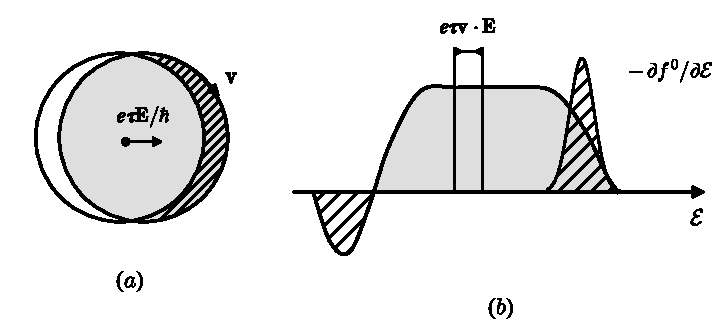
\includegraphics[width=0.72\textwidth]{fig_122.pdf}
\caption*{图 122\quad (a)移位的 费米面。(b)移位的 费米分布。}
\end{figure}

另一个值得注意之点是，式 (7.27) 可以写成
\begin{equation*}
f_{\mathbf{k}}=f^{0}(\mathcal{E}_{\mathbf{k}}-e\tau\,\mathbf{v}_{\mathbf{k}}\cdot\mathbf{E}),\tag{7.28}
\end{equation*}
就好像态 $\mathbf{k}$ 中的电子获得了大小为
\begin{equation*}
\delta\mathcal{E}_{\mathbf{k}}=e\tau\,\mathbf{v}_{\mathbf{k}}\cdot\mathbf{E}.\tag{7.29}
\end{equation*}
的能量。这正是经典图像中它应有的行为：假如它以速度 $\mathbf{v}_{\mathbf{k}}$ 在电场 $\mathbf{E}$ 中运动一段平均时间 $\tau$，就会得到这样一份能量。处理输运问题的\emph{分子运动论方法}（kinetic method）正是以这一论证为基础的。在与杂质两次碰撞之间获得的这份额外能量，等价于沿场方向的一个\emph{漂移速度}（drift velocity）$\delta\mathbf{v}$，它满足
\begin{equation*}
\delta\mathbf{v}\cdot\frac{\partial\mathcal{E}}{\partial\mathbf{v}}=e\mathbf{v}\cdot\mathbf{E}\,\tau,\tag{7.30}
\end{equation*}
即
\begin{equation*}
\delta\mathbf{v}=\frac{e\tau v}{mv}\,\mathbf{E},\tag{7.31}
\end{equation*}
这是对质量为 $m$ 的经典粒子而言的。

如果每单位体积有 $n$ 个粒子，则净电流密度为
\begin{equation*}
\mathbf{J}=ne\,\delta\mathbf{v},\tag{7.32}
\end{equation*}
而把式 (7.31)、(7.32) 与式 (7.22) 相比较，就得到
\begin{equation*}
\sigma=\frac{ne^{2}\tau}{m}.\tag{7.33}
\end{equation*}

很容易证明，对自由电子气而言，式 (7.25) 与式 (7.33) 给出相同的结果；但对金属来说，前者在原理上是好得多的公式。从线性响应理论的观点看，把它写成
\begin{equation*}
\sigma=\frac{1}{3}\,j_{F}^{2}\tau\,\mathcal{N}(\mathcal{E}_{F})\tag{7.34}
\end{equation*}
甚至还要更好，这表明电导率只取决于 费米能级处电子的性质，而不取决于金属中电子的总数。金属的高电导率应归因于 费米分布顶端的少数电子所携带的大电流 $j_{F}=ev_{F}$，而不是归因于可以被拉动而缓慢漂移的自由电子具有很高的总密度。

基本公式 (7.25) 还表明，如果自由 费米面的面积因与区边界的相互作用而减小，情况会怎样；它还把使 费米面上电子的有效速度降低的晶格效应考虑在内。这类效应在诸如 Bi 这样的金属中肯定可以观察到。

另一方面，分子运动论公式 (7.33) 则适用于半导体，其中 $n$ 是自由载流子的数目。习惯上写成
\begin{equation*}
\sigma=n\,|e|\,\mu,\tag{7.35}
\end{equation*}
其中
\begin{equation*}
\mu=\frac{|e|\tau}{m}\tag{7.36}
\end{equation*}
是载流子的\emph{迁移率}（mobility）。更一般地，人们假定电子和空穴分别对电流作出贡献，于是写成
\begin{equation*}
\sigma=n_{e}|e|\,\mu_{e}+n_{h}|e|\,\mu_{h},\tag{7.37}
\end{equation*}
并分别定义\emph{电子迁移率}（electron mobility）与\emph{空穴迁移率}（hole mobility）。

比如说，从式 (7.20) 出发推导式 (7.35) 并不困难：对 $f^{0}$ 采用类似式 (4.32) 的经典分布函数，并计算像式 (4.36) 那样的积分。这时要假定 $\tau$ 可以是能量的函数，于是求得其平均值（用以代入式 (7.36)）为
\begin{equation*}
\bar{\tau}=\frac{2}{3kT}\int\mathcal{E}\,\tau(\mathcal{E})\,e^{-\mathcal{E}/kT}\mathcal{N}(\mathcal{E})\,\mathrm{d}\mathcal{E}\;\bigg/\int e^{-\mathcal{E}/kT}\mathcal{N}(\mathcal{E})\,\mathrm{d}\mathcal{E},\tag{7.38}
\end{equation*}
其中 $\mathcal{N}(\mathcal{E})$ 是载流子所在的那个特定能带中的态密度。于是
\begin{equation*}
\mu_{e}=\frac{|e|\,\bar{\tau}_{e}}{m_{e}},\tag{7.39}
\end{equation*}
其中 $m_{e}$ 是电子的有效质量——空穴亦然。这些公式表明，迁移率可以是温度的函数；随着 $T$ 升高，分布展宽，平均弛豫时间随之改变。在金属中，$\tau$ 随能量的变化关系影响不大；重要的只是 $\tau(\mathcal{E}_{F})$ 的数值。

\section{弛豫时间的计算}

我们至今还没有求解积分方程 (7.16)。事实上，它最普遍的可能解应当写成
\begin{equation*}
g_{\mathbf{k}}=\left(-\frac{\partial f^{0}}{\partial\mathcal{E}}\right)e\mathbf{E}\cdot\boldsymbol{\Lambda}(\mathbf{k}),\tag{7.40}
\end{equation*}
其中 $\boldsymbol{\Lambda}(\mathbf{k})$ 是在 费米面上每一点 $\mathbf{k}$ 处定义的一个矢量。我们的初等解 (7.19) 相当于取
\begin{equation*}
\boldsymbol{\Lambda}(\mathbf{k})=\tau\,\mathbf{v}_{\mathbf{k}},\tag{7.41}
\end{equation*}
这表明 $\boldsymbol{\Lambda}$ 是电子的\emph{矢量平均自由程}（vector mean free path）。在一般情形下，$\boldsymbol{\Lambda}(\mathbf{k})$ 的大小可以变化，而且在 费米面上还可以偏离 $\mathbf{v}_{\mathbf{k}}$ 的方向。

有时人们假定可以写成
\begin{equation*}
\boldsymbol{\Lambda}(\mathbf{k})=\tau(\mathbf{k})\,\mathbf{v}_{\mathbf{k}},\tag{7.42}
\end{equation*}
其中 $\tau(\mathbf{k})$ 是一个在 费米面上变化的\emph{各向异性弛豫时间}（anisotropic relaxation time）。然而容易证明，这并不总是积分方程的完整解——而且也不存在计算函数 $\tau(\mathbf{k})$ 的直接方法。

事实上，唯一简单的解就是初等解 (7.19)。假设我们把它作为 $g_{\mathbf{k}}$ 代入 (7.16)，并且还假定散射是弹性的，即
\begin{equation*}
Q(\mathbf{k},\mathbf{k}')\,\mathrm{d}\mathbf{k}'=\delta(\mathcal{E}-\mathcal{E}')\,\mathcal{Q}(\mathbf{k},\mathbf{k}')\,\mathrm{d}\Omega'\,\mathrm{d}E,\tag{7.43}
\end{equation*}
其中 $\mathrm{d}\Omega'$ 是散射后 $\mathbf{k}'$ 的方向上的立体角元（$\mathbf{k}'$ 的大小现在由它必须与 $\mathbf{k}$ 具有相同能量 $\mathcal{E}'$ 这一要求所确定）。

在两边消去能量的 delta 函数之后，我们得到
\begin{equation*}
\mathbf{v}_{\mathbf{k}}\cdot\mathbf{E}=\tau\int(\mathbf{v}_{\mathbf{k}}-\mathbf{v}_{\mathbf{k}'})\cdot\mathbf{E}\,\mathcal{Q}(\mathbf{k},\mathbf{k}')\,\mathrm{d}\Omega'\tag{7.44}
\end{equation*}
积分在 费米面上进行。这是一个泛函关系，它对 $\mathcal{Q}(\mathbf{k},\mathbf{k}')$ 的形式施加了若干条件。容易证明：当我们有球形 费米面、$|\mathbf{v}_{\mathbf{k}}|$ 为常数，并且
\begin{equation*}
\mathcal{Q}(\mathbf{k},\mathbf{k}')=\mathcal{Q}(\theta);\tag{7.45}
\end{equation*}
也就是说，当散射概率仅是两个波矢之间夹角的函数时，关系式 (7.44) 便能够成立。这个证明只不过是球面三角学的一道练习题，我们把它留给读者。

如果这些条件得到满足，我们立刻得到
\begin{equation*}
\frac{1}{\tau}=\int(1-\cos\theta)\,\mathcal{Q}(\theta)\,\mathrm{d}\Omega'.\tag{7.46}
\end{equation*}
这表明，弛豫时间反比于一个对所有过程的散射概率的积分——但带上了因子 $(1-\cos\theta)$ 的权重，向大角散射倾斜。正如在 (7.44) 中所见，这个因子来自 $(\mathbf{v}_{\mathbf{k}}-\mathbf{v}_{\mathbf{k}'})\cdot\mathbf{E}$；重要的并不是电子被散射这件事，而是在此过程中电子速度沿电场方向的分量改变了多少。

我们可以借助数密度为 $N_{i}$ 的杂质的微分散射截面 $\sigma(\theta)$ 来表达散射概率：平均自由程 $\Lambda$ 由下式给出
\begin{equation*}
\frac{1}{\Lambda}=N_{i}\,2\pi\int_{0}^{\pi}(1-\cos\theta)\,\sigma(\theta)\sin\theta\,\mathrm{d}\theta.\tag{7.47}
\end{equation*}

\section{杂质散射}

现在，有了 (6.70)、(7.25) 和 (7.47)，我们就具备了从第一性原理出发计算含带电杂质的自由电子金属之电导率所需的材料。我们通常把它表示成\emph{电阻率}
\begin{align*}
\rho&=\frac{mv_{F}}{ne^{2}\Lambda}\\
&=\frac{mv_{F}}{ne^{2}}\,N_{i}\,2\pi\int_{0}^{\pi}(1-\cos\theta)\left(\frac{2mZe^{2}}{\hbar^{2}}\right)^{2}\frac{\sin\theta\,\mathrm{d}\theta}{(K^{2}+\lambda^{2})^{2}}\\
&=\frac{mv_{F}}{ne^{2}}\,N_{i}\,2\pi\left(\frac{2mZe^{2}}{\hbar^{2}\lambda^{2}}\right)^{2}\int_{0}^{1}\frac{8z^{3}\,\mathrm{d}z}{\left\{1+(2k_{F}/\lambda)^{2}z^{2}\right\}^{2}}.\tag{7.48}
\end{align*}
这里我们利用了散射的几何关系，即 $K=2k_{F}\sin\frac{1}{2}\theta$，并在被积函数中令 $z=\sin\frac{1}{2}\theta$。

(7.48) 中的积分作为 $(2k_{F}/\lambda)$ 的函数很容易算出——我们不打算写出精确的公式。要注意的要点是：一个带电杂质的行为就像一个半径为
\begin{equation*}
R\sim\left(\frac{2mZe^{2}}{\hbar^{2}\lambda^{2}}\right)\tag{7.49}
\end{equation*}
的几何障碍物；由 (5.22) 和 (3.6)，它与原子球的半径相当。我们还注意到，这一电阻与温度无关，而且应当按价差 $Z$ 的平方变化（\emph{Linde 定则}，Linde's rule）。

实际上，由 (7.48) 给出的电阻太大了。更好的做法是采用分波公式 (5.40) 来计算散射截面。对 $\theta$ 的积分可以做出来；我们得到
\begin{equation*}
\frac{1}{\Lambda}=N_{i}\,\frac{4\pi}{k_{F}^{2}}\sum_{l=1}^{\infty}l\sin^{2}(\eta_{l-1}-\eta_{l}).\tag{7.50}
\end{equation*}
然后可以确定各相移，使之满足 Friedel 求和规则 (5.43)。任何在 费米能级附近具有 $d$ 共振（§§5.5、6.10）的过渡金属杂质，显然必定产生很大的\emph{剩余电阻率}（residual resistivity），此时 $\eta_{2}\sim\pi/2$。对磁性杂质而言，依赖于自旋的 s--d 相互作用还会导致\emph{电阻极小}（resistance minimum），即 \emph{Kondo 效应}（Kondo effect），这将在 §10.6 中讨论。

要计算半导体中与带电杂质散射相联系的迁移率，我们可以采用与 (7.48) 本质上相同的论证。此时弛豫时间实际上是依赖于能量的：
\begin{equation*}
\frac{1}{\tau(\mathcal{E})}=N_{i}\,v\cdot 2\pi\left(\frac{Ze^{2}}{\epsilon\mathcal{E}}\right)^{2}\int_{0}^{1}\frac{\frac{1}{2}z^{3}\,\mathrm{d}z}{\left\{z^{2}+\lambda^{2}\hbar^{2}/8m^{*}\mathcal{E}\right\}^{2}},\tag{7.51}
\end{equation*}
其中 $\lambda$——现在由 (5.26) 给出——被假定远小于热激发所容许的 $k$ 值范围。

我们若把这个积分算出来，就会发现它随 $\mathcal{E}$ 只变化得很慢：$\tau$ 通过因子 $\mathcal{E}^{2}/v\propto\mathcal{E}^{\frac{3}{2}}m^{*\frac{1}{2}}$ 依赖于载流子的能量。当我们把它代入 (7.38) 时，实际上发现这相当于用平均值 $kT$ 代替 $\mathcal{E}$。于是，对于杂质散射，
\begin{equation*}
\mu\propto T^{\frac{3}{2}}m^{*\frac{3}{2}}.\tag{7.52}
\end{equation*}
（译注：按式 (7.51) 的 $\tau\propto\mathcal{E}^{3/2}m^{*1/2}$ 代入 (7.38)、(7.39)，
这类公式确实非常粗糙，但“迁移率应当随温度升高而增大”这一普遍的定性论证是可靠的。我们的意思是：载流子气越热，平均载流子就运动得越快，也就越不容易被带电杂质散射。

\section{“理想”电阻}

计算金属的所谓\emph{“理想”电阻}（'ideal' resistance）——即来源于晶格热振动之散射的电阻——是一个更为复杂的问题。我们只能把论证的主要线索勾画出来。

作为一级近似，我们可以利用 §6.14 中引入的形变势原理。电子感受到一个涨落势，其大小为
\begin{equation*}
\delta\mathcal{E}=\tfrac{2}{3}\mathcal{E}_{F}\,\Delta,\tag{7.53}
\end{equation*}
其中 $\Delta$ 是局域的、随热涨落的体膨胀。因此，电阻应当正比于密度的均方涨落；按照经典统计力学的一个熟知原理，它由下式给出
\begin{equation*}
\overline{\Delta^{2}}=NkT\beta,\tag{7.54}
\end{equation*}
其中 $\beta$ 是压缩率。

如果用声速 $s$ 和密度 $D$ 来表示，就有
\begin{equation*}
\overline{\Delta^{2}}=\frac{NkT}{Ds^{2}}=\frac{kT}{Ms^{2}},\tag{7.55}
\end{equation*}
其中 $M$ 是一个离子的质量。这个结果更为人们熟悉的形式是如下的一般关系
\begin{equation*}
\rho_{t}\propto\frac{T}{M\Theta^{2}}\tag{7.56}
\end{equation*}
它表明电阻正比于绝对温度。电阻随原子质量以及随 Debye 温度 $\Theta$（如 §2.4 中那样，$\Theta$ 与 $s$ 成正比）的变化，大体上与实验相符。

为了在这一结果上有所改进，我们可以采用 (6.87)，即晶格中每个离子的有效微分截面。由 (7.47) 我们得到平均自由程
\begin{equation*}
\frac{1}{\Lambda_{t}}=N\,2\pi\int_{0}^{\pi}\sigma_{a}(\theta)\,N|\mathbf{K}\cdot\mathbf{U}_{\mathbf{q}}|^{2}(1-\cos\theta)\sin\theta\,\mathrm{d}\theta,\tag{7.57}
\end{equation*}
其中 $\sigma_{a}(\theta)$ 是“自由原子”的微分散射截面。

假设我们只考虑 N 过程，即散射矢量 $\mathbf{K}$ 等于声子波矢 $\mathbf{q}$ 的过程。在 (2.109) 与 (2.110) 中已经算出因子 $|\mathbf{K}\cdot\mathbf{U}_{\mathbf{q}}|^{2}$。在高温下
\begin{align*}
N|\mathbf{K}\cdot\mathbf{U}_{\mathbf{q}}|^{2}&\approx\frac{kTK^{2}}{M\nu_{\mathbf{q}}^{2}}\\
&\approx\frac{kT}{Ms^{2}}\\
&\approx\frac{\hbar^{2}q_{D}^{2}\,kT}{Mk^{2}\Theta^{2}}\tag{7.58}
\end{align*}
——以 Debye 温度表出。实际上，这就是 (7.54) 与 (7.55) 中的 $\overline{\Delta^{2}}$。

由于 (7.58) 与 $\mathbf{K}$ 无关，也就是与散射角 $\theta$ 无关，我们可以把这个积分单独算出来，并写成
\begin{equation*}
\frac{1}{\Lambda_{t}}=N\bar{\sigma}_{a}\,\frac{\hbar^{2}q_{D}^{2}\,kT}{Mk^{2}\Theta^{2}},\tag{7.59}
\end{equation*}
其中
\begin{equation*}
\bar{\sigma}_{a}\equiv 2\pi\int\sigma_{a}(\theta)\,(1-\cos\theta)\sin\theta\,\mathrm{d}\theta,\tag{7.60}
\end{equation*}
即孤立原子的总散射截面，并以因子 $(1-\cos\theta)$ 计及沿场方向动量的变化。

利用 Lindemann 熔化公式 (2.117)，这个公式还可以进一步约化。我们得到
\begin{equation*}
\frac{1}{\Lambda_{t}}\approx N\bar{\sigma}_{a}\cdot\tfrac{2}{3}x_{m}^{2}\,\frac{T}{T_{m}},\tag{7.61}
\end{equation*}
其中 $x_{m}$ 是 (2.117) 中量级为 0.2 的常数，$T_{m}$ 是熔化温度。我们还可以再往前走一点，假定一个离子的散射截面与带电杂质的散射截面大体相同。对 (7.49) 稍作变换，就得到大致如下的结果
\begin{equation*}
\Lambda_{t}\sim 50a\,\frac{T_{m}}{T},\tag{7.62}
\end{equation*}
其中 $a^{3}$ 是一个晶胞的体积；金属中电子的平均自由程在熔点处应当具有晶格常数 50 倍的量级。这并不严格正确——但作为数量级的估计还是站得住脚的。

要得到电阻本身，我们应当把 (7.59) 或 (7.62) 与 (7.33) 结合起来，写成
\begin{equation*}
\rho_{t}=\frac{mv_{F}}{ne^{2}\Lambda_{t}},\tag{7.63}
\end{equation*}
这对自由电子气近似地成立。这些公式使我们粗糙的函数关系 (7.56) 有了具体的数字。

但在低温下情况要更复杂。(7.58) 这个结构因子是在经典统计的假设下算出来的。如果进入低温区，我们就必须把比如 $(kT/\hbar\nu_{\mathbf{q}})$ 换成由 (2.46) 给出的 $\bar{n}_{\mathbf{q}}$。\footnote{零点能并不进入这个公式；要证明这一点，需要对散射作细致的分析，把声子的发射过程与吸收过程区分开来。}我们得到
\begin{equation*}
N|\mathbf{K}\cdot\mathbf{U}_{\mathbf{q}}|^{2}\approx\frac{kT}{Ms^{2}}\left\{\frac{\hbar\nu_{\mathbf{q}}/kT}{\exp(\hbar\nu_{\mathbf{q}}/kT)-1}\right\}.\tag{7.64}
\end{equation*}

(7.57) 积分中的这个因子起到了在角度变量上设置切断的作用。当我们需要吸收或发射频率高得无法被热激发的声子时，散射概率迅速下降；也就是说，对于满足
\begin{equation*}
\hbar\nu_{\mathbf{q}}>kT.\tag{7.65}
\end{equation*}
的散射，我们实际上不予考虑。

对于 Debye 模型以及球形 费米面上的 N 过程，这种情况发生于如下的 $q$ 值和散射角 $\theta$，使得
\begin{equation*}
\frac{q}{2k_{F}}=\sin\tfrac{1}{2}\theta>\frac{q_{D}}{2k_{F}}\,\frac{T}{\Theta}.\tag{7.66}
\end{equation*}

如果我们假定 $\sigma_{a}(\theta)$ 并非随 $\theta$ 急剧变化的函数，因而可以作为一个常数提到积分之外，就能相当精确地计算平均自由程。于是 (7.57) 给出
\begin{equation*}
\frac{1}{\Lambda_{t}}=N\bar{\sigma}_{a}\,\frac{\hbar^{2}q_{D}^{2}\,kT}{Mk^{2}\Theta^{2}}\left(\frac{T}{\Theta}\right)^{4}\int_{0}^{\Theta/T}\frac{4z^{4}\,\mathrm{d}z}{(e^{z}-1)},\tag{7.67}
\end{equation*}
其中我们已令
\begin{equation*}
z=\frac{\hbar\nu_{\mathbf{q}}}{kT}=\left(\frac{q}{q_{D}}\right)\left(\frac{\Theta}{T}\right).\tag{7.68}
\end{equation*}

\begin{figure}[H]
\centering
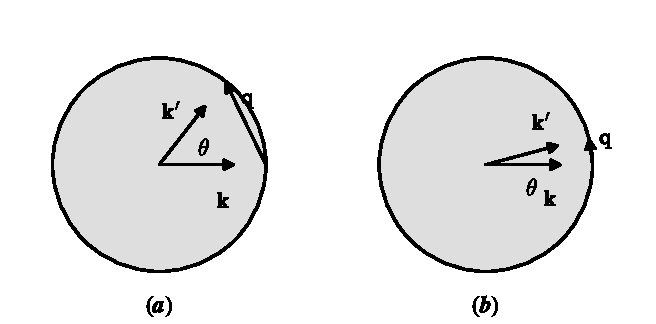
\includegraphics[width=0.72\textwidth]{fig_123.pdf}
\caption*{图 123\quad 电子--声子 N 过程：(a)高温下；(b)低温下。}
\end{figure}

在高温下，$\Theta/T$ 很小，积分趋于 $(\Theta/T)^{4}$，我们就回到了 (7.59)。在低温下，积分趋于一个常数 124.4，于是电阻正比于 $T^{5}$。“理想”电阻的这种强烈的温度依赖性是一种典型的量子效应，可与 Debye $T^{3}$ 比热定律相比拟。

我们可以看出发生了什么。有效散射截面是一个对角度的积分，带有因子
\begin{equation*}
(1-\cos\theta)\sin\theta\,\mathrm{d}\theta=8\sin^{3}\tfrac{1}{2}\theta\,\mathrm{d}(\sin\tfrac{1}{2}\theta)\tag{7.69}
\end{equation*}
因而对 (7.64) 所提示的切断非常敏感。如果取 (7.66) 作为切断角，我们就应当发现一个正比于
\begin{equation*}
\int_{0}^{(q_{D}/2k_{F})(T/\Theta)}8\sin^{3}(\tfrac{1}{2}\theta)\,\mathrm{d}(\sin\tfrac{1}{2}\theta)\propto\left(\frac{T}{\Theta}\right)^{4},\tag{7.70}
\end{equation*}
的因子，这正是 (7.67) 中出现的那一个。长波声子作为电阻的来源效果很差，因为它们只能把电子散射过一个小角——而这个角随温度成比例地减小。

把 (7.67) 与 (7.63) 结合起来得到的公式，就是所谓的 \emph{Bloch--Grüneisen 定律}（Bloch--Grüneisen law）。许多金属在低温下近似遵从它——但不应对它过分拘泥于字面，理由如下：

（i）我们假定了电子被弹性散射。这并不真实——但如果我们按照电子--声子的产生与湮没过程作一个形式上的分析，并计入电子失去或获得的能量，就得到几乎相同的结果。(7.67) 中的积分变为
\begin{equation*}
\int_{0}^{\Theta/T}\frac{4z^{5}\,\mathrm{d}z}{(e^{z}-1)(1-e^{-z})},
\end{equation*}
它在 $T$ 很小和很大时的渐近行为都与 (7.67) 相同。

（ii）Debye 谱的假设只是一种方便的过分简化。纵模与横模各自的贡献应当分别考虑。

（iii）函数 $\sigma_{a}(\theta)$ 不是常数，因此不能把它从 (7.57) 的积分号下提出来。计算 $\sigma_{a}(\theta)$ 的公式由 (6.89) 与 (6.93) 给出。特别是，当 $\theta$ 超过大约 $20^{\circ}$--$30^{\circ}$ 以后，$\sigma_{a}(\theta)$ 趋于减小——这也对电阻随温度的变化产生影响。

（iv）最严重的误差在于忽略了 U 过程。如 §2.7 所示，如果 $\mathbf{K}$ 越出了某个 Brillouin 区的边界，我们就应当写成
\begin{equation*}
\mathbf{q}=\mathbf{K}-\mathbf{g},\tag{7.71}
\end{equation*}
其中 $\mathbf{g}$ 是一个倒格矢。在我们的公式 (7.57) 中，并没有什么特殊理由使这样的 $\mathbf{K}$ 值无法达到；原子的散射截面作为角度的函数会一直延伸到 $\theta=\pi$，那将使 $K=2k_{F}$，大于 Debye 极限 $q_{D}$。

U 过程给电阻造成的困难只不过在于，它们会引起复杂的几何问题。即使在高温下，如果把 (7.71) 代入 (7.58)，我们也会发现“结构因子”不再与散射角无关：它包含一个额外的因子 $K^{2}/q^{2}$，这个因子可以远大于 1。我们可以在图 124(a) 中看到这一点，其中 $K$ 显然远大于 $q$。对于这样大的 $\theta$ 值，微分散射截面 $\sigma_{a}(\theta)$ 也许很小——但对电阻的贡献却被因子 $(1-\cos\theta)$ 重重地加权。

某些 U 过程所需要的很小的 $q$ 值，在我们考虑电阻随温度的变化时也很重要。正如 (7.66) 所表明的，直到温度降到很低，这些过程才被“冻结”。如果把图 124(a) 的矢量三角形在重复区图式中重新画出，这一点可以看得更清楚。这时，一个倒逆过程所要求的 $q$ 的最小值，显然就是一个区中的 费米面与其在相邻区中的重复像之间的最小距离。

\begin{figure}[H]
\centering
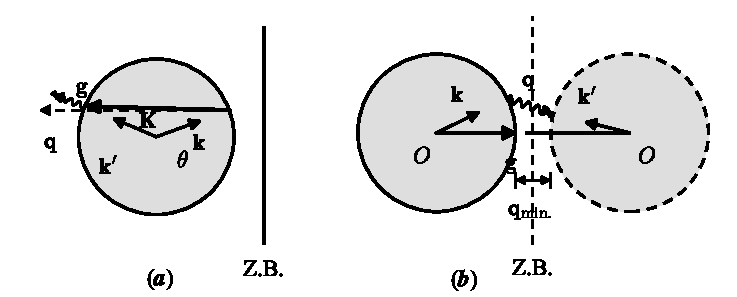
\includegraphics[width=0.72\textwidth]{fig_124.pdf}
\caption*{图 124\quad 电子--声子 U 过程：(a)在自由电子球上；(b)在重复区图式中。}
\end{figure}

如果 费米面朝区边界的方向鼓出，那么 $q$ 的最小值就减小——于是 (7.57) 中带因子 $K^{2}/q^{2}$ 的贡献将得到增强。的确，看起来几乎就好像：倘若 费米面碰到区边界，$\rho_{i}$ 中就会出现一个奇点——不过，正如 §6.13 中指出的，对于这样的过程，电子--声子相互作用的矩阵元自动为零。

U 过程对电阻的贡献没有简单的公式。不过，给出 (7.56) 和 (7.67) 的那些同样的普遍因素仍在起作用——尽管后一个表达式作为精确的理论结果并不成立。我们能够理解这一现象的全部物理特征，但必须依靠繁冗的数值计算才能得到答案。举一点为例：按照 (6.93)，原子在 $\mathbf{K}$ 值大（即 $\theta$ 大）时的有效截面依赖于 $\mathcal{V}'$ 的大小，即赝原子的“芯赝势”（'core pseudo-potential'）。这应当反映在电阻的大小上——但电阻对 $\mathcal{V}'$ 的敏感，既可能来自它使 费米面畸变、使区边界附近的波函数相混合的方式，也同样可能来自它对散射矩阵元的直接贡献。

\begin{figure}[H]
\centering
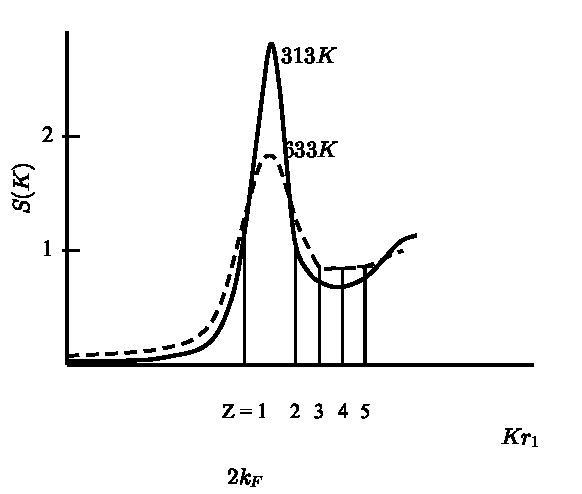
\includegraphics[width=0.72\textwidth]{fig_125.pdf}
\caption*{图 125\quad 液态金属的典型结构因子，图中标出不同价数下的 $2k_{F}$，以及温度依赖性。}
\end{figure}

对\emph{液态}金属的类似计算实际上要容易得多。假定一个 N.F.E. 模型是合理的，此时 (6.88)、(6.91)、(7.25) 和 (7.47) 引导我们得到公式
\begin{equation*}
\rho_{L}=\frac{3\pi}{4}\,\frac{1}{\hbar^{2}e^{2}v_{F}^{2}k_{F}^{4}}\,\frac{1}{N}\int_{0}^{2k_{F}}|w_{s}(K)|^{2}\,S(K)\,K^{3}\,\mathrm{d}K.\tag{7.72}
\end{equation*}
在这个表达式中，起实质性作用的要素是赝原子形状因子 $|w_{s}(K)|^{2}$ 和液体结构因子 $S(K)$，后者可以用中子或 X 射线衍射在实验上测定。事实上，大多数液态金属中原子的排列方式如此相似，以致在按原子半径标度之后，$S(K)$ 可以近似地用一条统一的标准曲线来表示（图 125）。在小的 $K$ 处，结构因子很小，因为原子分布在密度上近乎均匀——事实上，经典公式 (7.54) 在这里仍然成立。但第一
配位壳层——即径向分布函数 $P(R)$ 中的近邻壳层（参见式 (2.103)）——在 $S(K)$ 中给出一个峰，越过此峰后 $S(K)$ 便在 1 附近振荡。在这张图上，Fermi 球的直径 $2k_{F}$ 依赖于价数 $Z$，因此 (7.72) 中的积分上限在碱金属中达不到 $S(K)$ 的峰，而当 $Z=2$ 时则落入其后的谷中。

由于没有能够产生 Brillouin 区等等的长程序，N 过程与 U 过程之间的区分便失去意义。尽管如此，几何因子 $K^{3}$ 使被积函数的权重强烈地偏向 $2k_{F}$ 附近的值，于是“芯”赝势 $\mathcal{V}'$ 再一次成为占主导的效应。金属熔化时电阻的增大，可以归结为结构因子在大 $K$ 处的变化——即从仍正比于 $T$ 的电子--声子 U 过程，变为来自 $S(K)$ 峰附近的散射；此峰已达 1 的量级，而且在更高的温度下实际上还可能减小。

\section{载流子迁移率}

半导体中载流子被晶格振动的散射，就其一般原理而言是一个简单得多的问题。因为载流子通常被认为集中在 $\mathbf{k}$ 空间的一个小区域内，即 $\mathcal{E}(\mathbf{k})$ 的某个极小值附近，散射中 $\mathbf{k}$ 矢量的可能改变很小。这使我们能够利用 §6.13 的形变势（deformation potential）。散射概率正比于
\begin{equation*}
|\mathcal{M}_{\mathbf{k}'\mathbf{k}}|^{2}\,\mathcal{N}(\mathcal{E})=\Bigl|\sum_{ij}\mathsf{W}^{0}_{ij}\,\mathcal{E}_{ij}\Bigr|^{2}\mathcal{N}(\mathcal{E}),\tag{7.73}
\end{equation*}
其中 $\mathsf{W}^{0}_{ij}$ 是弹性波中应变某个分量的振幅，而 $\mathcal{E}_{ij}$ 是形变势张量的一个分量。

由于 $\mathbf{k}'-\mathbf{k}$ 很小，我们可以对弹性波诸模采用经典统计：如同 (7.54) 那样，
\begin{equation*}
\overline{|\mathsf{W}^{0}_{ij}|^{2}}\propto kT.\tag{7.74}
\end{equation*}
于是，正比于 (7.73) 之倒数的弛豫时间将按如下方式变化
\begin{equation*}
\frac{1}{\tau(\mathcal{E})}\propto T\mathcal{E}^{\frac{1}{2}}m^{*\frac{3}{2}},\tag{7.75}
\end{equation*}
因为态密度是能量和“有效质量”二者的函数（参见式 (4.33)）。把它代入 (7.38) 和 (7.39)，我们得到
\begin{equation*}
\mu\propto T^{-\frac{3}{2}}m^{*-\frac{5}{2}}.\tag{7.76}
\end{equation*}
小有效质量带来的“报酬”是非常高的。

然而，即使引入矩阵元等等，这个理论也仍然太简单。许多半导体的电子极小值不止一个——用行话说，有很多\emph{能谷}（many valleys）（§6.6）——而借助大波矢声子进行的谷间散射十分重要。关系式 (7.76) 在实践中并不很令人满意。

在半导体中，发射或吸收声子时载流子能量的变化不可忽略。它对低场下载流子迁移率的影响不大，但却是\emph{高场}（high-field）输运现象中的主导机制。例如，设想在一个薄的导电样品两端加上几伏的电动势。在两极之间运动的载流子必须把这些能量作为 Joule 热放出——实际上就是发射若干个声子。在金属中，电子--声子两次散射之间的平均自由程非常短（参见式 (7.62)），以致在这个机制失效之前，样品本身早就被气化了。然而在好的半导体中，相当温和的电场（例如 1000 V/cm）就能使能量转移过程过载，于是电子的能量分布可能不再像 (7.38) 所假设的那样处于晶格温度下的平衡。随之发生的\emph{热电子}（hot electron）现象在理论上相当复杂，因为它细致地依赖于电子--声子矩阵元、声学支与光学支的频谱以及固体的电子能带结构。不过，总的效果是偏离 Ohm 定律，趋向于载流子电流几乎与 $E$ 无关的状态。

这个关于电导的讨论还假定晶体动量 $\mathbf{k}$ 是电子态的一个好量子数。在某些情形下——例如在玻璃、非晶态半导体或补偿杂质带中（§§4.2、5.9、6.7）——最好把载流子描述为\emph{定域}（localized）在材料中的各个位置上。这时，导电只能通过热激活的\emph{跳跃}（hopping）从一个位置到另一个位置来实现，同时发射或吸收一个合适的声子以容许这一跃迁。

\section{普遍输运系数}

现在假定样品中除了电场之外还存在温度梯度。忽略尺寸和形状效应，Boltzmann 方程 (7.14) 就成为
\begin{equation*}
\left(-\frac{\partial f^{0}}{\partial\mathcal{E}}\right)\mathbf{v}_{\mathbf{k}}\cdot\left\{\frac{\mathcal{E}(\mathbf{k})-\zeta}{T}(-\nabla T)+e\left(\mathbf{E}-\frac{1}{e}\nabla\zeta\right)\right\}=-\left.\frac{\partial f_{\mathbf{k}}}{\partial t}\right]_{\text{scatt.}}\tag{7.77}
\end{equation*}
我们所做的一切，只是把 (7.16) 中的 $\mathbf{E}$ 换成一个更为复杂的、依赖于 $\mathbf{k}$ 的矢量函数。如果弛豫时间得以存在的条件仍然成立——正如 §7.3 中讨论过的——那么我们就知道解的形式：
\begin{equation*}
f_{\mathbf{k}}-f^{0}_{\mathbf{k}}=\left(-\frac{\partial f^{0}}{\partial\mathcal{E}}\right)\tau\mathbf{v}_{\mathbf{k}}\cdot\left[e\left(\mathbf{E}-\frac{1}{e}\nabla\zeta\right)+\frac{\mathcal{E}(\mathbf{k})-\zeta}{T}(-\nabla T)\right].\tag{7.78}
\end{equation*}
我们可以把它代入一个像 (7.20) 那样的积分中来计算电流，
\begin{align*}
\mathbf{J}&=\frac{1}{4\pi^{3}}\,\frac{e^{2}\tau}{\hbar}\iint\mathbf{v}_{\mathbf{k}}\mathbf{v}_{\mathbf{k}}\left(-\frac{\partial f^{0}}{\partial\mathcal{E}}\right)\frac{\mathrm{d}S}{v_{\mathbf{k}}}\,\mathrm{d}\mathcal{E}\cdot\left(\mathbf{E}-\frac{1}{e}\nabla\zeta\right)\\
&\quad+\frac{1}{4\pi^{3}}\,\frac{e^{2}\tau}{\hbar}\iint\mathbf{v}_{\mathbf{k}}\mathbf{v}_{\mathbf{k}}\left(\frac{\mathcal{E}-\zeta}{T}\right)\left(-\frac{\partial f^{0}}{\partial\mathcal{E}}\right)\frac{\mathrm{d}S}{v_{\mathbf{k}}}\,\mathrm{d}\mathcal{E}\cdot(-\nabla T).\tag{7.79}
\end{align*}
这表明，温度梯度 $\nabla T$ 即使单独作用也会产生电流——这正是存在温差电效应（thermo-electric effect）的证据。

但是，温度梯度最重要的效应是产生\emph{热}流。我们也许会把它看作一种能量通量，
\begin{equation*}
2\int f_{\mathbf{k}}\,\mathcal{E}(\mathbf{k})\,\mathbf{v}_{\mathbf{k}}\,\mathrm{d}\mathbf{k}.
\end{equation*}
（译注：按式 (7.78) 代入 (7.20)，第二项似应为 $e\tau/\hbar$；原书印作 $e^{2}\tau$。）
但这并不正确。“热”是“内能”减去“自由能”。电子的自由能是 $\zeta$，即它的化学势。因此，处于态 $\mathbf{k}$ 的电子所携带的热量是 $\mathcal{E}(\mathbf{k})-\zeta$。更严格的分析证实，热通量的总量（每单位体积）必须由下式计算：
\begin{equation*}
\mathbf{U}=2\int f_{\mathbf{k}}\{\mathcal{E}(\mathbf{k})-\zeta\}\,\mathbf{v}_{\mathbf{k}}\,\mathrm{d}\mathbf{k}.\tag{7.80}
\end{equation*}

在写下 $\mathbf{U}$ 的表达式之前，我们还可以注意到，(7.78) 中含有一个 $\nabla\zeta$ 项——这一项来自电子气温度的改变所引起的化学势变化（参见式 (4.23)）。但在电学性质的普通测量中，任何这类 $\zeta$ 的梯度都应当计入电路中所测得的诸电动势之内。我们将径直略去这一项，假定它的任何效应都已包含在 $\mathbf{E}$——即“观测到的”电场——之中。

由 (7.78)、(7.79) 和 (7.80)，我们可以构造出如下的普遍输运方程
\begin{align*}
\mathbf{J}&=e^{2}\mathsf{K}_{0}\cdot\mathbf{E}+\frac{e}{T}\,\mathsf{K}_{1}\cdot(-\nabla T),\tag{7.81a}\\
\mathbf{U}&=e\,\mathsf{K}_{1}\cdot\mathbf{E}+\frac{1}{T}\,\mathsf{K}_{2}\cdot(-\nabla T),\tag{7.81b}
\end{align*}
其中各系数（其实是张量，不过这只是为了抽象的普遍性而已）定义为
\begin{equation*}
\mathsf{K}_{n}\equiv\frac{1}{4\pi^{3}}\,\frac{\tau}{\hbar}\iint\mathbf{v}\mathbf{v}\,(\mathcal{E}-\zeta)^{n}\left(-\frac{\partial f^{0}}{\partial\mathcal{E}}\right)\frac{\mathrm{d}S}{v}\,\mathrm{d}\mathcal{E}.\tag{7.82}
\end{equation*}
这些系数可以借助我们关于 Fermi 函数对能量积分的普遍定理 (4.21) 来求值：
\begin{equation*}
\int\Phi(\mathcal{E})\left(-\frac{\partial f^{0}}{\partial\mathcal{E}}\right)\mathrm{d}\mathcal{E}=\Phi(\zeta)+\tfrac{1}{6}\pi^{2}(kT)^{2}\left[\frac{\partial^{2}\Phi(\mathcal{E})}{\partial\mathcal{E}^{2}}\right]_{\mathcal{E}=\zeta}+\cdots,\tag{7.83}
\end{equation*}
这里 $\Phi(\mathcal{E})$ 本身是能量面 $\mathcal{E}(\mathbf{k})=\mathcal{E}$ 上的一个积分。但这并不带来特殊的困难。

正如 (7.21) 中那样，我们有
\begin{equation*}
\mathsf{K}_{0}=\frac{1}{4\pi^{3}}\,\frac{\tau}{\hbar}\int\mathbf{v}\mathbf{v}\,\frac{\mathrm{d}S_{F}}{v}.\tag{7.84}
\end{equation*}
现在设想 $\mathsf{K}_{0}(\mathcal{E})$ 是 (7.84) 在某个能量为 $\mathcal{E}$（而非 费米能级处）的面上的取值。对于 $\mathsf{K}_{2}$，我们必须考虑 $\Phi(\mathcal{E})=(\mathcal{E}-\zeta)^{2}\mathsf{K}_{0}(\mathcal{E})$，它在 $\mathcal{E}=\zeta$ 处为零，于是在 (7.83) 的第二项中只剩下
\begin{equation*}
\mathsf{K}_{2}=\tfrac{1}{3}\pi^{2}(kT)^{2}\mathsf{K}_{0}(\zeta)\tag{7.85}
\end{equation*}
而 $\mathsf{K}_{1}$ 的表达式则化为
\begin{equation*}
\mathsf{K}_{1}=\tfrac{1}{3}\pi^{2}(kT)^{2}\left[\frac{\partial}{\partial\mathcal{E}}\,\mathsf{K}_{0}(\mathcal{E})\right]_{\mathcal{E}=\zeta},\tag{7.86}
\end{equation*}
这在原理上要更复杂一些。

(7.81a) 中 $\mathbf{E}$ 的系数当然就是电导率——即我们在等温条件（$\nabla T=0$）下应当测得的电流。我们只是重新确认了 (7.23)；我们写下
\begin{equation*}
\boldsymbol{\sigma}=e^{2}\mathsf{K}_{0},\tag{7.87}
\end{equation*}
而当张量由于具有立方对称性而约化为标量时，还有与之等价的关系式。我们实际上就是利用 (7.87) 用已知的电导率来表示 $\mathsf{K}_{0}$。

\section{热导率}

(7.81b) 是热流方程，其中温度梯度的系数就是我们应当称为电子气的热导率（thermal conductivity）的量。

实际上，这并不完全正确。我们做实验时并不会保持 $\mathbf{E}=\mathbf{0}$。更方便的做法是把样品接成开路，使 $\mathbf{J}=\mathbf{0}$。由 (7.81a)，这意味着沿导线将建立起一个电场
\begin{equation*}
\mathbf{E}=\frac{1}{e^{2}}\,\mathsf{K}_{0}^{-1}\mathsf{K}_{1}\,\frac{e}{T}\cdot\nabla T\tag{7.88}
\end{equation*}
把它代入 (7.81b)，我们得到
\begin{align*}
\mathbf{U}&=\frac{1}{T}\,\mathsf{K}_{1}\mathsf{K}_{0}^{-1}\mathsf{K}_{1}\cdot\nabla T-\frac{1}{T}\,\mathsf{K}_{2}\cdot\nabla T\\
&=\frac{1}{T}\,(\mathsf{K}_{2}-\mathsf{K}_{1}\mathsf{K}_{0}^{-1}\mathsf{K}_{1})\cdot(-\nabla T),\tag{7.89}
\end{align*}
我们应当把它与
\begin{equation*}
\mathbf{U}=\boldsymbol{\kappa}\cdot(-\nabla T)\tag{7.90}
\end{equation*}
中的热导率 $\kappa$ 等同起来。但对金属而言这一修正可以忽略，于是
\begin{equation*}
\kappa=\frac{1}{T}\,\mathsf{K}_{2}.\tag{7.91}
\end{equation*}
而根据 (7.85) 和 (7.87)，此式可以写成
\begin{equation*}
\kappa=\frac{\pi^{2}}{3}\,\frac{k^{2}}{e^{2}}\,T\sigma,\tag{7.92}
\end{equation*}
这个关系称为 Wiedemann--Franz 定律。它是一个老结果，而且非常容易理解。在电传导中，每个电子携带电荷 $e$，受力 $e\mathbf{E}$ 的作用；单位场强下的电流正比于 $e^{2}$。在热传导中，每个电子携带其热能 $kT$，受“热力”$k\nabla T$ 的作用；单位温度梯度下的热流正比于 $k^{2}T$。这两个输运系数之比必须具有 $k^{2}T/e^{2}$ 的量级；因子 $\frac{1}{3}\pi^{2}$ 来自如下事实：我们处理的只是 费米面上服从 费米统计的电子。

容易证明，这个定律是非常普遍的。倘若 (7.40) 成立——也就是说，倘若散射的效应只用一个在 费米面上变化的矢量平均自由程就能定义——这一定律便会成立。但它要求散射是\emph{弹性}的。

为了证明这一点，让我们考察热传导条件下实际分布函数的形式。由 (7.78)，
\begin{equation*}
f_{\mathbf{k}}-f^{0}_{\mathbf{k}}=\left(-\frac{\partial f^{0}}{\partial\mathcal{E}}\right)\left(\frac{\mathcal{E}-\zeta}{T}\right)\tau\,\mathbf{v}_{\mathbf{k}}\cdot(-\nabla T).\tag{7.93}
\end{equation*}
让我们看一看 费米分布的一个截面。如图 126 所示，在 $f^{0}$ 上加上一个像 (7.93) 那样的表达式，其效果是使 $\mathbf{v}_{\mathbf{k}}\cdot(-\nabla T)$ 为正的一侧的分布展宽，而在另一侧则使分布变窄。

我们可以把它解析地表示出来：
\begin{align*}
f_{\mathbf{k}}&=f^{0}_{\mathbf{k}}-(\tau\,\mathbf{v}_{\mathbf{k}}\cdot\nabla T)\,\frac{\partial f^{0}}{\partial T}\\
&=f^{0}(T-\tau\,\mathbf{v}_{\mathbf{k}}\cdot\nabla T).\tag{7.94}
\end{align*}
沿 $\nabla T$ 为负的方向运动的电子，即沿温度梯度下行方向运动的电子，要“热”出这样一个数量：
\begin{equation*}
\delta T=-\tau\,\mathbf{v}_{\mathbf{k}}\cdot\nabla T.\tag{7.95}
\end{equation*}
沿相反方向运动的电子，则比电子气的平均温度“冷”。

\begin{figure}[H]
\centering
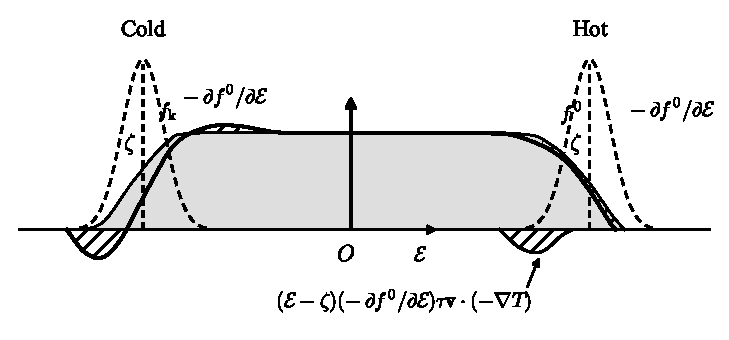
\includegraphics[width=0.72\textwidth]{fig_126.pdf}
\caption*{图 126\quad 热传导中的 费米分布。}
\end{figure}

的确，这正是我们按分子运动论的推理所应得出的结论。从方向 $\mathbf{v}$ 过来、到达温度为 $T$ 的区域的电子，已经走过了一段距离 $\tau v$。它们离开的那个区域——即它们上一次经受使其热化的碰撞的区域——将处于温度 $T+\delta T$。因此，这些电子要“热”出一个量 $\delta T$。

于是，在热传导实验中没有净的电子通量——没有净的电荷通量。之所以有热流，是因为有“热”电子向一个方向行进，同时有同等数目的“冷”电子向相反方向行进。图 127(a) 中粗略地画出了这一情形。右边有一些被激发到 费米能级以上的电子；左边则有一些凝聚入 费米面之内的电子。

现在考虑这个分布可以通过哪些散射方式而弛豫。我们可以把一个热电子沿 Fermi 球一直散射过去，使其方向反转。我们称之为\emph{水平过程}（horizontal process）。这类散射同样也是降低电导率的有效过程，如图 127(b) 所示。这类过程是弹性的——对它们而言 Wiedemann--Franz 定律成立。

但也存在\emph{竖直}跃迁：一个“热”电子失去它的全部多余能量，落到 费米能级以下。这类过程对电导率的影响很小——但在热传导中，它在削减热流方面与大角散射同等重要。

\begin{figure}[H]
\centering
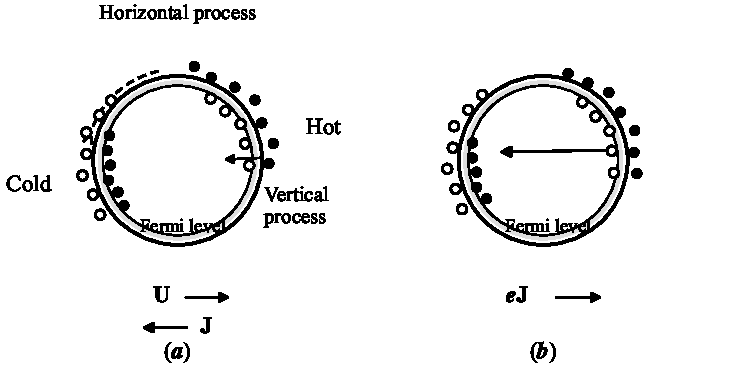
\includegraphics[width=0.72\textwidth]{fig_127.pdf}
\caption*{图 127\quad 电子分布与散射过程：(a) 热传导中；(b) 电传导中。}
\end{figure}

按定义，竖直跃迁是\emph{非弹性}的。杂质散射不会发生这种跃迁，由杂质散射引起的热阻服从 Wiedemann--Franz 定律。换言之，由于 $\rho$ 为常数，$\kappa\propto T$。在高温下的声子散射中，竖直跃迁也不十分重要，因为那时电子能够获得或失去的最大能量就是一个声子的最大能量，即 $k\Theta$。它小于 费米分布相对于 费米能级的展宽 $kT$：结果表明，在高温极限下，对“理想”电阻而言 Wiedemann--Franz 定律同样成立。由于 $\rho_{i}$ 正比于 $T$，我们发现 $\kappa_{i}$ 应当趋于一个常数。

但在低温下，电子平均获得或失去的能量就是该温度下声子的平均能量，即它必须具有 $kT$ 的量级。这恰好足以使电子穿过热层——恰好足以把一个“热”电子变成“冷”的。

对这种情形推导一个公式，显然需要仔细研究产生或吸收声子的各个具体过程。但是，如果我们假定现在所有散射过程在削减热流方面都同等有效，就可以大致看出会发生什么。也就是说，在像 (7.46) 那样计算“弛豫时间”时，我们现在略去因子 $(1-\cos\theta)$，正是这个因子顾及了电子速度沿场方向分量的变化。

但这个因子 $(1-\cos\theta)$ 在低温下曾在积分 (7.70) 中贡献了 $2\sin^{2}\frac{1}{2}\theta$。于是，在我们的“截止”近似中应当去掉一个因子 $(T/\Theta)^{2}$。在像 (7.67) 那样的计算中，“热导率弛豫时间”将得出为
\begin{equation*}
\frac{1}{\tau}\propto\frac{T^{3}}{M\Theta^{4}}\tag{7.96}
\end{equation*}
而不是电导率中所得到的 $T^{5}$ 定律。把它代入 (7.91)、(7.85) 和 (7.84)（即在把热导率与电导率相比较时总是要计入的、正比于 $T$ 的 Wiedemann--Franz 因子），我们得到
\begin{equation*}
\kappa_{i}\propto\frac{M\Theta^{4}}{T^{2}}.\tag{7.97}
\end{equation*}
这在实际中被观察到——在 Debye 温度以下，电子--声子过程给出如下形式的 Lorenz 比（Lorenz ratio）：
\begin{equation*}
\frac{\kappa_{i}}{\sigma_{i}T}\propto\left(\frac{T}{\Theta}\right)^{2}\tag{7.98}
\end{equation*}
而不是 Wiedemann--Franz 定律 (7.92) 所要求的常数值 $(\tfrac{1}{3}\pi^{2})(k/e)^{2}$。但在极低温度下，剩余电阻（§7.4）来自杂质的弹性散射，这个比值便回到 Lorenz 比 (7.92)。

当然，还必须考虑 U 过程对热阻率的贡献，但这又是一个复杂的计算问题。

\section{温差电效应}

普遍关系 (7.81) 表明，电流与热流之间存在交互效应。例如，设想在一个开路的样品中建立温度梯度。在 (7.81a) 中令 $\mathbf{J}=\mathbf{0}$（这里悄悄换成标量系数），我们得到
\begin{align*}
\mathbf{E}&=\frac{1}{eT}\,(\mathsf{K}_{0}^{-1}\mathsf{K}_{1})\,\nabla T\\
&=Q\nabla T;\tag{7.99}
\end{align*}
这时将观测到一个电动势。

为了演示并测量这个效应，必须用两种金属 $A$ 和 $B$ 组成一个闭合回路，两个接头处于不同的温度 $T_{1}$ 和 $T_{2}$，并在某个中间点（温度 $T_{0}$）接入一个伏特计。回路中的电动势定义为 $\mathbf{E}$ 沿导线全长的积分
\begin{align*}
\phi&=\int_{0}^{1}E_{B}\,\mathrm{d}x+\int_{1}^{2}E_{A}\,\mathrm{d}x+\int_{2}^{0}E_{B}\,\mathrm{d}x\\
&=\int_{2}^{1}Q_{B}\,\frac{\partial T}{\partial x}\,\mathrm{d}x+\int_{1}^{2}Q_{A}\,\frac{\partial T}{\partial x}\,\mathrm{d}x\\
&=\int_{T_{1}}^{T_{2}}(Q_{A}-Q_{B})\,\mathrm{d}T.\tag{7.100}
\end{align*}
回路中产生的电压看起来像是两个接头温度之差、以及两种金属的\emph{绝对温差电功率}（absolute thermo-electric power）$Q$ 之差的函数。这就是著名的 Seebeck 效应。

\begin{figure}[H]
\centering
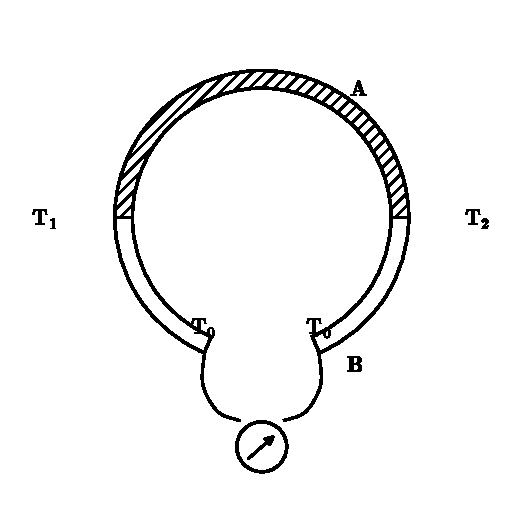
\includegraphics[width=0.72\textwidth]{fig_128.pdf}
\caption*{图 128\quad Seebeck 效应。}
\end{figure}

但是还有另一种现象，它与 (7.81) 中出现的量 $\mathsf{K}_{1}$ 相联系。设想我们使一个如图 129 那样的回路保持 $\nabla T=\mathbf{0}$。由 (7.81a)，我们有
\begin{equation*}
\mathbf{U}=e\,\mathsf{K}_{1}\,\mathbf{E},\qquad\mathbf{J}=e^{2}\mathsf{K}_{0}\,\mathbf{E},\tag{7.101}
\end{equation*}
于是
\begin{align*}
\mathbf{U}&=\frac{1}{e}\,\mathsf{K}_{0}^{-1}\mathsf{K}_{1}\,\mathbf{J}\\
&=\Pi\,\mathbf{J}.\tag{7.102}
\end{align*}
现在用电池在回路中驱动一个电流 $J$。在支路 $A$ 中将有一个热流 $\Pi_{A}J$；在支路 $B$ 中则将有另一个热流 $\Pi_{B}J$。在接头处，热的平衡必须重新建立；热通量 $(\Pi_{A}-\Pi_{B})J$ 将在一个接头处放出，而在另一个接头处吸收。一个接头将变热，另一个变冷。这就是 Peltier 效应。

正如从 (7.99) 和 (7.102) 所看到的，\emph{Peltier 系数}与绝对温差电功率有以下关系：
\begin{equation*}
\Pi=QT.\tag{7.103}
\end{equation*}
这并非偶然。它是温差电学的 \emph{Kelvin 关系}（Kelvin relations）之一，也是不可逆过程热力学的 Onsager 关系的一个特例。实质上，方程 (7.81) 若用 $\mathbf{J}$ 和 $\mathbf{U}/T$ 来表达，就必须具有一个对称的矩阵——这解释了为什么 $\mathsf{K}_{1}$ 作为系数出现了两次。还有另一种
\begin{figure}[H]
\centering
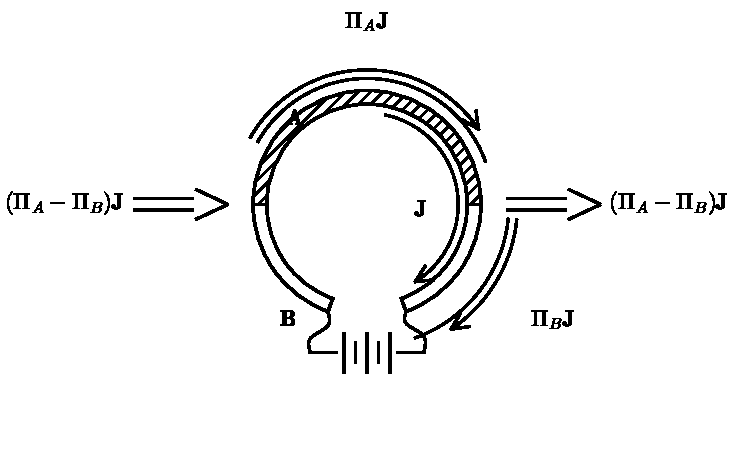
\includegraphics[width=0.72\textwidth]{fig_129.pdf}
\caption*{图 129\quad Peltier 效应。}
\end{figure}
温差电效应——\emph{Thomson 效应}（Thomson effect），它在同时载有热流和电流的回路中被观察到——不过这个效应的系数已经包含在普遍关系 (7.81) 之中。

至于温差电功率的实际数值，我们援引 (7.86) 和 (7.87)：
\begin{equation*}
Q=\frac{\pi^{2}}{3}\,\frac{k}{e}\,kT\left[\frac{\partial\ln\sigma(\mathcal{E})}{\partial\mathcal{E}}\right]_{\mathcal{E}=\zeta},\tag{7.104}
\end{equation*}
其中 $\sigma(\mathcal{E})$ 意指“在一个假想的、费米能级位于 $\mathcal{E}$ 处的金属中电导率所取的值”。把这个公式应用于各种情形下电导率的计算结果，在原则上足够容易（尽管在实践中往往复杂而不成功）。

例如，设想我们写出
\begin{equation*}
\sigma(\mathcal{E})=n(\mathcal{E})\,e\,\mu(\mathcal{E})\tag{7.105}
\end{equation*}
即以一个随能量变化的载流子密度和一个有效载流子迁移率来表述。于是我们有
\begin{equation*}
Q=\frac{\pi^{2}}{3}\,\frac{k}{e}\,kT\left[\frac{\mathcal{N}(\mathcal{E})}{n}+\frac{\partial\ln\mu(\mathcal{E})}{\partial\mathcal{E}}\right]_{\mathcal{E}=\zeta}.\tag{7.106}
\end{equation*}
第一项很容易理解。正如 §4.7 中所见，“每电子比热”是
\begin{equation*}
C_{\text{el.}}=\frac{\pi^{2}}{3}\,k^{2}T\,\frac{\mathcal{N}(\mathcal{E}_{F})}{n}.\tag{7.107}
\end{equation*}
因此，Peltier 系数 $QT$ 就是“每电子热”与电子电荷之比——正如 (7.100) 所提示的那样。

之所以出现迁移率的导数，是因为我们必须顾及电子电流按能量分布的方式。于是，如果 $\mu(\mathcal{E})$ 随能量增大，那么电流中有很高的比例是由能量较高的电子承载的，而这些电子按比例携带着较大的热流。

当然，对于金属，(7.105) 并不合理；应当像 (7.25) 那样用 费米面面积和平均自由程来表示电导率，或者像 (7.34) 那样用态密度、Fermi 电流和弛豫时间来表示。对于自由电子系统，两种作法的结果相同；但要正确解释金属或合金中的温差电现象，就必须小心选择模型，使得上述各种因素随能量的变化都能得到正确的评估。磁性杂质所产生的巨大温差电功率（§10.6）就是这类效应的一个极端例子。值得注意，电荷 $e$ 按惯例取负值，因此 $Q$ 应当为负——尤其是因为 $\mu(\mathcal{E})$ 倾向于随 $\mathcal{E}$ 而增大；较快的电子不那么容易被散射。

在半导体中，这类公式不能令人满意。我们必须回到各系数的定义 (7.82)，并且不能再像 (7.83) 那样利用 Fermi 函数的性质。特别地，$\mathsf{K}_{1}$ 的积分具有如下形式
\begin{equation*}
\int(\mathcal{E}-\zeta)\,f_{\mathbf{k}}\,\mathbf{v}_{\mathbf{k}}\,\mathrm{d}\mathbf{k},\tag{7.108}
\end{equation*}
其中将含有对应于 §4.6 中 $\zeta_{e}$ 的“热”——即载流子的能量，不是从最近的带边量起，而是从真正的 费米能级量起。于是，温差电功率中有一个形如下式的贡献
\begin{equation*}
Q_{e}\sim\frac{1}{T}\,\frac{\zeta_{e}}{e}\tag{7.109}
\end{equation*}
此外还有一项通常较小的、来自 $\mu(\mathcal{E})$ 行为的贡献。

如果我们的半导体主要含有“空穴”，那么就应当
也应当有类似的结果，只是改由 $\zeta_{h}$ 扮演“每个载流子所携带的热量”的角色，并且此时电荷为正。当两类载流子同时存在时，我们得到的将是一个平均的温差电功率（thermo-electric power），介于电子的负贡献与空穴的正贡献之间而取得平衡，各自按其在总电流中所占的份额加权。

有趣的是，不妨想一想：对于金属，在考虑“空穴球”时，我们有哪两种可供选择的处理办法。如同 §6.6，我们可以把它看作一个电子的 费米面，其 $e$ 为负，但具有一个奇特的性质：电子的面积、速度和弛豫时间全都随能量的增加而\emph{减小}，于是在式 (7.104) 中 $\partial\ln\sigma(\mathcal{E})/\partial\mathcal{E}$ 也是负的，从而 $Q$ 为正。更自然的做法是把它看作一个由“空穴”组成的球，空穴的数目和迁移率随其“能量”自中心向外而\emph{增加}，但它们携带的是正电荷。两种办法的结果相同。

\begin{figure}[H]
\centering
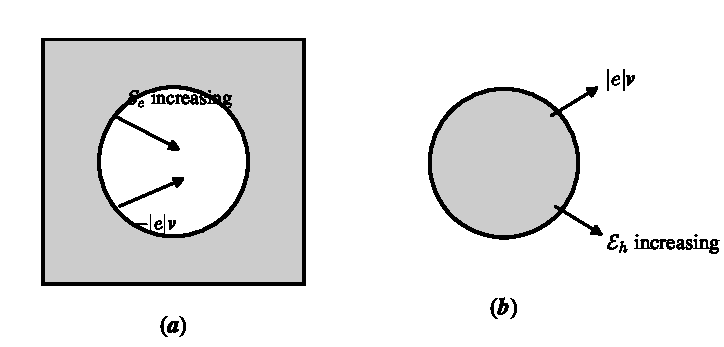
\includegraphics[width=0.72\textwidth]{fig_130.pdf}
\caption*{图 130\quad 计算温差电功率的两种可供选择的模型：(a)电子 费米面；(b)“空穴”费米面。}
\end{figure}

\section{晶格热传导}

在电绝缘体和半导体中，仍可能有经由格波的良好的热传导。这是一个极为复杂的课题，我们只对它作一点粗浅的研究。

设想我们把声子当作一种粒子气体来处理。初等分子运动论中已经证明，热导率为
\begin{equation*}
\kappa=\tfrac{1}{3}\,Cv\Lambda,\tag{7.110}
\end{equation*}
其中 $C$ 是比热，$v$ 是速度，$\Lambda$ 是载流子的平均自由程（mean free path）。

在高温下，我们可以认为声子具有其通常的比热 $3Nk$，如式 (2.60)；也可以认为它们以声速 $s$ 行进。但要计算 $\Lambda$，我们还须作某些粗略的近似。其中最简单的一种，与 §7.5 中估计电子平均自由程时所用的论证相仿。

让我们回忆一下，晶格的膨胀 $\Delta$ 会局部地改变声速，相对改变量为
\begin{equation*}
\frac{\delta s}{s}=\gamma\Delta,\tag{7.111}
\end{equation*}
其中 $\gamma$ 是 Grüneisen 常数。这个常数在式 (2.120) 中讨论热膨胀理论时已经定义过。

密度的局域热涨落将引起散射，其强度正比于这个量的均方。与式 (7.59) 直接比较，可以写出
\begin{equation*}
\frac{1}{\Lambda}\sim\frac{\gamma^{2}\overline{\Delta^{2}}}{a},\tag{7.112}
\end{equation*}
亦即
\begin{equation*}
\Lambda\sim\frac{Ds^{2}}{NkT}\,\frac{a}{\gamma^{2}},\tag{7.113}
\end{equation*}
其中 $a$ 是具有晶格常数量级的一个长度。于是，利用式 (7.110) 并略去数值因子，便得到
\begin{equation*}
\kappa\sim\frac{Ds^{3}}{\gamma^{2}T}\,a,\tag{7.114}
\end{equation*}
其中 $D$ 是密度。这个公式有意思之处在于，除了 $a$ 以外，式中出现的全是宏观量。

改写式 (7.113) 的另一种方式是用熔化温度来表示：如式 (7.62)，我们有
\begin{equation*}
\Lambda\sim\frac{20}{\gamma^{2}}\,\frac{T_{m}}{T}\,a.\tag{7.115}
\end{equation*}

这些公式在函数行为和数量级上是合理的；晶格热导率对绝对温度倒数的依赖关系已被很好地理解，尽管其余因子是相当粗糙的。

然而，这只在高于 Debye 温度的高温下才成立，而且实际情形远不像表面上那样简单。事实是，“密度的热涨落”与“携带热流的声子”并无本质区别，整个系统应当像 §2.10 中那样用声子--声子相互作用来分析。

于是我们得到一个非常特别的结果。设想只有晶体动量守恒的声子--声子 N 过程。设想我们建立起一个在模式 $\mathbf{q}$ 中含有 $n_{\mathbf{q}}$ 个声子的态——即一个具有净晶体动量
\begin{equation*}
\mathbf{P}=\sum_{\mathbf{q}}n_{\mathbf{q}}\hbar\mathbf{q}\tag{7.116}
\end{equation*}
的态。这时，声子--声子 N 过程并不改变 $\mathbf{P}$ 的值。因此，与 $\mathbf{P}$ 相联系的任何净热流都不会耗散：热导率必须为无穷大。

实际上，我们得到的是声子沿样品的\emph{对流}（convection）。正如在\emph{流动的气体}中那样，粒子之间的碰撞允许动量发生交换，并在气体内部建立起某种程度的局域平衡；除了通过与器壁的相互作用而间接起作用之外，它们并不会减慢热的质量输运。当然，对于气体中的\emph{热传导}，条件就完全不同了；我们刻意坚持不许粒子有任何质量输运，这时碰撞才变得重要起来，因为朝一个方向运动的“热”粒子把能量交给朝相反方向运动的“冷”粒子。但在声子气体中，“粒子”并没有净的守恒性，所以我们不能强加这样的条件。携带热量所需的额外声子在热端产生，流向冷端，并在那里被消灭。

晶体热导率之所以有限，是由于 U 过程（U-process）的存在。由于在这类过程中晶体动量不守恒，量 (7.116) 不能保持恒定，热流于是被耗散。这种情形下热阻的计算相当复杂，但其结果在高温下正与式 (7.114) 和 (7.115) 相合。这个非常朴素的近似方法结果证明是有道理的。

但在低温下，声子--声子 U 过程引起的电阻迅速降为零。我们回忆一下（§2.11）波矢所满足的几何条件
\begin{equation*}
\mathbf{q}+\mathbf{q}'=\mathbf{q}''+\mathbf{g},\tag{7.117}
\end{equation*}
以及频率所满足的能量条件
\begin{equation*}
\nu+\nu'=\nu''.\tag{7.118}
\end{equation*}
这样，$\mathbf{q}''$ 必须足够大，使其能量等于 $\mathbf{q}$ 与 $\mathbf{q}'$ 的能量之和；但要发生 U 过程，这些矢量之和必须越出第一 Brillouin 区，因此 $\mathbf{q}''$ 的长度不可能比 $\frac{1}{2}\mathbf{g}$ 小很多。在 Debye 模型中，这意味着
\begin{figure}[H]
\centering
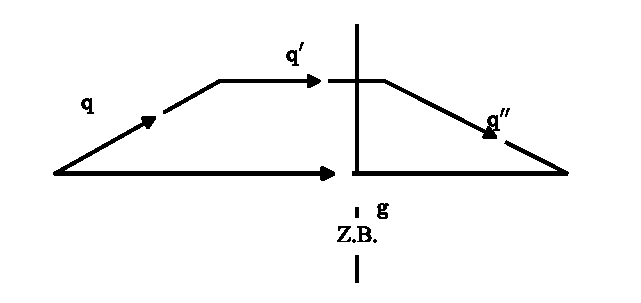
\includegraphics[width=0.72\textwidth]{fig_131.pdf}
\caption*{图 131\quad 声子--声子 U 过程。}
\end{figure}
\begin{equation*}
q''\geqslant\beta q_{D},\tag{7.119}
\end{equation*}
其中 $\beta$ 是一个分数，量级为 $\frac{1}{2}$ 或 $\frac{2}{3}$。换句话说，
\begin{equation*}
\hbar\nu''\geqslant\beta k\Theta.\tag{7.120}
\end{equation*}
形如式 (7.118) 的 U 过程出现的概率，正比于相应声子模式占据数的乘积
\begin{align*}
n_{\mathbf{q}}\,n_{\mathbf{q}'}&\approx\exp(-\hbar\nu/kT)\exp(-\hbar\nu'/kT)\\
&\approx\exp(-\hbar\nu''/kT)\\
&\approx\exp(-\beta\Theta/kT)\tag{7.121}
\end{align*}
在低温下它迅速趋于零。我们说倒逆散射被“冻结”了，热导率按
\begin{equation*}
\kappa\sim T^{n}\exp\left(\frac{\beta\Theta}{T}\right),\tag{7.122}
\end{equation*}
趋于无穷，其中 $n$ 是一个依赖于模型细节的指数。

实际发生的情形是：声子的平均自由程变得可以与晶体的尺寸相比拟。设想我们处理的是一根直径为 $D$ 的棒。于是在式 (7.110) 中可以取
\begin{equation*}
\Lambda=D,\tag{7.123}
\end{equation*}
从而
\begin{equation*}
\kappa\propto T^{3}D,\tag{7.124}
\end{equation*}
这是因为低温下比热服从 $T^{3}$ 定律（§2.4）。这个 $T^{3}$ \emph{尺寸效应}（size effect）在实验上有确凿的证据。

然而，还存在使声子受到散射的其他机制。即使在“完美”晶体中，原子也并非全都等价；对每一种化学元素来说，通常都是一些不同质量的同位素的混合。这些质量上的差别能够散射声子。我们很容易——比如用初等弹性理论——证明 \emph{Rayleigh 公式}：密度为 $D$ 的介质中一个点质量 $\delta M$ 对波数为 $q$ 的波的散射截面为
\begin{equation*}
\sigma(q)=\frac{q^{4}}{4\pi D^{2}}\,(\delta M)^{2}.\tag{7.125}
\end{equation*}
倘若晶体中每个原子的质量都可能偏离平均值这么多，那么声子的平均自由程将为
\begin{align*}
\Lambda(q)&=\frac{4\pi NM^{2}}{q^{4}(\delta M)^{2}}\\
&=\left(\frac{M}{\delta M}\right)^{2}\frac{4\pi a}{(aq)^{4}},\tag{7.126}
\end{align*}
其中 $N=1/a^{3}$。

$\Lambda(q)$ 随 $q$ 的强烈变化现在成了一个难题。自然的做法是把式 (7.110) 加以推广，写成
\begin{equation*}
\kappa=\frac{1}{3}\int C(q)\,v(q)\,\Lambda(q)\,\mathrm{d}\mathbf{q}\tag{7.127}
\end{equation*}
把各种模式的贡献加起来。但这会在 $q\to 0$ 处导致一个奇异性：在那里比热 $C(q)$ 和速度 $v(q)$ 实际上是常数，而 $\Lambda(q)\propto q^{-4}$；于是，对长波模式的分布利用类似于 (2.56) 的 Debye 谱，便得到
\begin{equation*}
\kappa\propto\int\frac{q^{2}\,\mathrm{d}q}{q^{4}}\sim\int_{0}\frac{\mathrm{d}q}{q^{2}}\to\infty\tag{7.128}
\end{equation*}

这一困难的解决是一个复杂的问题，但论证的实质是：即使在低温下，晶体中也总有强烈的声子--声子 N 过程在进行。这些过程本身并不产生热阻，但它们倾向于使各种模式彼此趋于平衡，因而不允许那些不受同位素强烈散射的长波模式携带过大的热流。

倘若声子--声子 N 过程确实非常强烈，我们就可以论证：式 (7.127) 中应当加以平均的量是 $1/\Lambda(q)$，这样积分才是有限的。在这种情形下，我们可以这样来估计用于分子运动论公式 (7.110) 中的平均自由程：假定在温度 $T$ 下只有一个“典型”的声子模式，其波矢为
\begin{equation*}
\overline{q}\sim\frac{T}{\Theta}\,q_{D}.\tag{7.129}
\end{equation*}
于是我们应当写出
\begin{equation*}
\Lambda\sim\Lambda(\overline{q})\propto T^{-4},\tag{7.130}
\end{equation*}
这将给出
\begin{equation*}
\kappa\propto\left(\frac{M}{\delta M}\right)^{2}\frac{1}{T}.\tag{7.131}
\end{equation*}
然而，更细致的分析——采用声子--声子相互作用的唯象模型——给出一种更复杂的行为：
\begin{equation*}
\kappa\propto\frac{M}{\delta M}\,\frac{1}{T^{1/2}}.\tag{7.132}
\end{equation*}
这与实验观测大致相符。

\section{声子曳引}

金属中的电子受声子散射。反过来，声子也受电子散射。一般说来，这种散射十分强烈，以致与电子气的热导率相比，晶格热传导就很难观察到了。

然而，在金属和半导体中，有一个由声子引起的重要电学效应。设想一根导线中流有电流。如式 (7.27) 所示，这可以描述为 费米面在 $\mathbf{k}$ 空间中的位移，位移量为 $(e\tau/\hbar)\mathbf{E}$。这个电子系统正在与声子相互作用。如果只有电子--声子相互作用，声子系统将力图与\emph{位移了的}电子系统达到平衡；也就是说，声子系统本身将倾向于在自己的动量空间中发生位移。

但声子系统的这样一种位移，对应于声子在真实空间中的“漂移”——也就是说，它对应于一个热流。设想声子的漂移速度与电子的漂移速度 (7.31) 相同。若 $C_{L}$ 是整个声子系统的比热，就会存在一个晶格热流
\begin{equation*}
\mathbf{U}_{L}\sim C_{L}T\,\delta\mathbf{v}.\tag{7.133}
\end{equation*}
但它又如式 (7.32) 那样伴随有一个电流。于是将有一个 Peltier 系数（参见式 (7.102)）
\begin{equation*}
\frac{U_{L}}{J}\sim\frac{C_{L}T}{ne},\tag{7.134}
\end{equation*}
亦即一个\emph{晶格温差电功率}（lattice thermo-electric power）
\begin{equation*}
Q_{L}\sim\frac{C_{L}}{ne}.\tag{7.135}
\end{equation*}

与普通的电子贡献 (7.106) 相比，这将是一个很大的效应；在后者中起作用的是电子的小得多的比热——如式 (7.107)——而不是晶格的比热。但当然，我们原本曾假定：除了电子--声子相互作用之外，声子不受任何其他机制的散射。在寻常温度下情况并非如此；那里存在着 §7.10 中讨论过的声子--声子 U 过程等等，它们使这个 \emph{Gurevitch 效应}（Gurevitch effect）大为减弱。

然而，在低温下，当声子--声子相互作用变得可以忽略时，\emph{声子曳引}（phonon drag）效应就很容易探测到了。在这种情况下，晶格比热按 $T^{3}$ 变化。对于单价金属，公式应当是
\begin{equation*}
Q_{L}\sim\frac{k}{e}\,\frac{4\pi^{4}}{5}\left(\frac{T}{\Theta}\right)^{3},\tag{7.136}
\end{equation*}
这是一个很大的\emph{负}温差电功率，其符号由电子电荷 $e$ 的符号决定。

但这并不总是实际观察到的情形，理由如下。“声子分布以电子的漂移速度一道被曳引”这一假设，依赖于电子--声子过程中晶体动量的守恒。考虑（图 132(a)）一个普通的 N 过程：电子由态 $\mathbf{k}$ 被散射到态 $\mathbf{k}'$，同时发射出一个声子。
\begin{figure}[H]
\centering
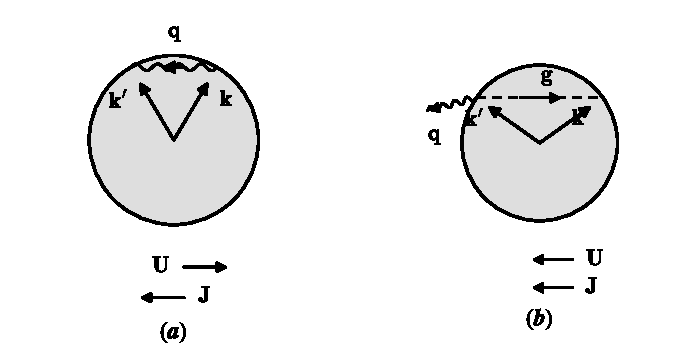
\includegraphics[width=0.72\textwidth]{fig_132.pdf}
\caption*{图 132\quad 电子对声子的曳引：(a)N 过程；(b)U 过程。}
\end{figure}
如果这一过程恰好使 $\mathbf{k}$ 沿场方向的分量反转，那么声子便沿该方向发射。于是，使电流减慢的这个过程，就产生了沿载流子运动方向运动的过剩声子。

现在考虑在电子--声子 U 过程中会发生什么。如图 132(b) 所示，声子倾向于沿与载流子电流\emph{相反}的方向被发射；矢量 $\mathbf{k}$、$\mathbf{k}'$ 与 $\mathbf{q}$ 之和必须给出大的倒格矢 $\mathbf{g}$。这样，声子分布就不随电子一道被“曳引”；它反而可能向相反的方向漂移。

因此，$Q_{L}$ 的实际符号可正可负，取决于在金属的“理想”电阻中 N 过程与 U 过程哪一种更为重要。这一效应显然非常敏感
% 注：本文件末句在原书 p259 末行处中断（sensitive to...），由 ch7_e（p260 起）直接续接，勿加标点。
于费米面的形状及其与区边界的距离，如 §7.5 中所讨论的那样。

应当指出，如果只有电子--声子 N 过程，那么式 (7.116) 的论证本来也适用：声子的曳引恰好抵偿电子的漂移，动量便不会有任何净的耗散。电导率将会增大，而且在没有剩余电阻时会趋于无穷。在实际金属中并未观察到这种现象，原因多半在于存在强烈的电子--声子 U 过程。

我们在这里给出的论证，也可以应用到半导体中的载流子上——如 §7.6 中那样，载流子会“曳引”与之相互作用的声子。这种效应在半导体中更大，因为只有波矢 $q$ 小的声子才散射载流子，而这些声子的平均自由程很长。在低温下，人们甚至能探测到温差电功率对样品尺寸的依赖。晶格温差电功率的符号与载流子的符号相同。

\section{Hall 效应}

让我们回到 Boltzmann 方程 (7.14)，只是现在除了电场之外还有磁场 $\mathbf{H}$。假定可以取一个弛豫时间，则该方程可写为
\begin{equation*}
e\mathbf{E}\cdot\mathbf{v}_{\mathbf{k}}\left(-\frac{\partial f^{0}}{\partial\mathcal{E}}\right)=\frac{g_{\mathbf{k}}}{\tau}+\frac{e}{\hbar c}\left(\mathbf{v}_{\mathbf{k}}\wedge\mathbf{H}\right)\cdot\frac{\partial g_{\mathbf{k}}}{\partial\mathbf{k}}.\tag{7.137}
\end{equation*}

这是关于 $\mathbf{k}$ 空间中函数 $g_{\mathbf{k}}$ 的一个微分方程。假设我们处理的是自由电子，对它们有
\begin{equation*}
\hbar\mathbf{k}=m\mathbf{v},\tag{7.138}
\end{equation*}
于是我们可以用速度而不用 $\mathbf{k}$ 来标记每个态。我们尝试如下形式的解
\begin{equation*}
g_{\mathbf{k}}=\left(-\frac{\partial f^{0}}{\partial\mathcal{E}}\right)\tau\,\mathbf{v}_{\mathbf{k}}\cdot e\mathbf{A},\tag{7.139}
\end{equation*}
其中 $\mathbf{A}$ 是一个有待确定的矢量。这当然是式 (7.19) 的类似式；在没有磁场时，$\mathbf{A}$ 结果就是 $\mathbf{E}$。

把式 (7.138) 和 (7.139) 代入式 (7.137)，得到
\begin{equation*}
\mathbf{v}\cdot\mathbf{E}=\mathbf{v}\cdot\mathbf{A}+\left(\frac{e\tau}{mc}\right)\left(\mathbf{v}\wedge\mathbf{H}\right)\cdot\mathbf{A},\tag{7.140}
\end{equation*}
显然，对 $\mathbf{v}$ 的一切值，下式都使它得到满足：
\begin{equation*}
\mathbf{E}=\mathbf{A}+\frac{e\tau}{mc}\,\mathbf{H}\wedge\mathbf{A}.\tag{7.141}
\end{equation*}

这是一个矢量方程，可以从中解出 $\mathbf{A}$。不难用初等几何证明（图 133），它的一个解是
\begin{equation*}
\mathbf{A}=\frac{\mathbf{E}-\dfrac{e\tau}{mc}\,\mathbf{H}\wedge\mathbf{E}}{1+\dfrac{e^{2}\tau^{2}}{m^{2}c^{2}}\,H^{2}}.\tag{7.142}
\end{equation*}
\begin{figure}[H]
\centering
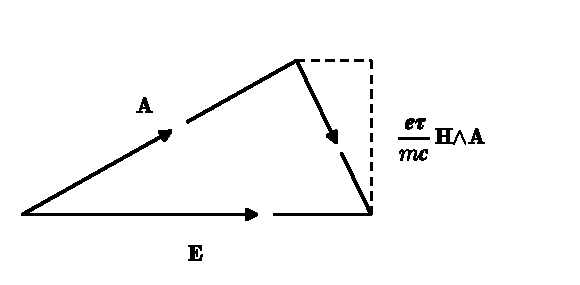
\includegraphics[width=0.72\textwidth]{fig_133.pdf}
\caption*{图 133\quad （原书此图无图注。）}
\end{figure}

但我们也可以直接从式 (7.141) 出发。取由式 (7.139) 给出的 $g_{\mathbf{k}}$，便容易看出电流就是简单地
\begin{equation*}
\mathbf{J}=\sigma_{0}\mathbf{A},\tag{7.143}
\end{equation*}
其中 $\sigma_{0}$ 是金属或半导体在没有磁场时的普通电导率；这由式 (7.19) 至 (7.23) 把 $\mathbf{E}$ 换成 $\mathbf{A}$ 即可得到。于是，由式 (7.141) 和 (7.143)
\begin{align*}
\mathbf{E}&=\frac{1}{\sigma_{0}}\mathbf{J}+\frac{e\tau}{mc}\,\mathbf{H}\wedge\frac{1}{\sigma_{0}}\mathbf{J}\\
&=\rho_{0}\mathbf{J}+\frac{e\tau}{mc}\,\rho_{0}\,\mathbf{H}\wedge\mathbf{J},\tag{7.144}
\end{align*}
其中 $\rho_{0}$ 是样品的普通电阻率。

这个方程表明，产生电流 $\mathbf{J}$ 所需的电场有两个分量。沿 $\mathbf{J}$ 的方向，即沿金属丝或金属带的长度方向，
\begin{equation*}
E_{\parallel}=\rho_{\parallel}J.\tag{7.145}
\end{equation*}
这告诉我们，样品的表观电阻不因磁场而改变；也就是说，\emph{没有磁致电阻（magneto-resistance）}。

但如果 $\mathbf{H}$ 垂直于 $\mathbf{J}$ 加上，就会有一个横向电场
\begin{equation*}
E_{H}=\frac{e\tau}{mc}\,\rho_{0}HJ.\tag{7.146}
\end{equation*}

这就是 \emph{Hall 效应（Hall effect）}。对自由电子，Hall 系数（Hall coefficient）为
\begin{align*}
R&=\frac{e\tau}{mc}\,\rho_{0}\\
&=\frac{1}{nec},\tag{7.147}
\end{align*}
这里我们用式 (7.33) 消去了弛豫时间。

这个结果——Hall 常数反比于载流子密度——用分子运动论的论证很容易理解。假定像式 (7.31) 中那样，载流子以速度 $\delta\mathbf{v}$ 漂移，那么它们将受到一个横越磁场方向的 Lorentz 力
\begin{equation*}
\frac{e}{c}\,\delta\mathbf{v}\wedge\mathbf{H}\tag{7.148}
\end{equation*}
的作用。恰好能够补偿这一侧向偏转的，正是一个横向电场
\begin{align*}
\mathbf{E}_{H}&=\frac{1}{c}\,\mathbf{H}\wedge\delta\mathbf{v}\\
&=\frac{1}{c}\,\mathbf{H}\wedge\frac{1}{ne}\mathbf{J}\tag{7.149}
\end{align*}
与 $1/n$ 成正比的原因在于：电流给定时，载流子密度越小，每个载流子就必须运动得越快，从而被磁场偏转得越厉害。

这个分子运动论的论证也告诉我们，为什么在这个简单情形下没有磁致电阻。横向的两个偏转效应恰好平衡，所以载流子在纵向电场的作用下沿金属丝行进时，就好像根本不存在磁场一样。

结果 (7.147) 实际上对任何球形的载流子集合都成立。假设我们在整个 费米面上写
\begin{equation*}
\hbar k_{F}=m^{*}v_{F}\tag{7.150}
\end{equation*}
这不过是用这个关系来定义参量 $m^{*}$。于是我们应当得到
\begin{equation*}
R=\frac{e\tau}{m^{*}c\sigma_{0}}\tag{7.151}
\end{equation*}
正如式 (7.146) 中那样。但这时（参照式 (7.25)）
\begin{align*}
\sigma_{0}&=\frac{e^{2}}{12\pi^{3}\hbar}\int\tau v_{F}\,\mathrm{d}S_{F}\\
&=\frac{e^{2}\tau}{12\pi^{3}}\int\frac{k_{F}\,\mathrm{d}S_{F}}{m^{*}}\\
&=\frac{e^{2}\tau}{m^{*}}\,\frac{1}{4\pi^{3}}\,\frac{4\pi}{3}\,k_{F}^{3}\\
&=\frac{ne^{2}\tau}{m^{*}},\tag{7.152}
\end{align*}
其中 $n$ 正是半径为 $k_{F}$ 的球内所包含的载流子数目。由式 (7.151) 和 (7.152) 便得到式 (7.147)，与 $\tau$ 和 $m^{*}$ 都无关。
\begin{figure}[H]
\centering
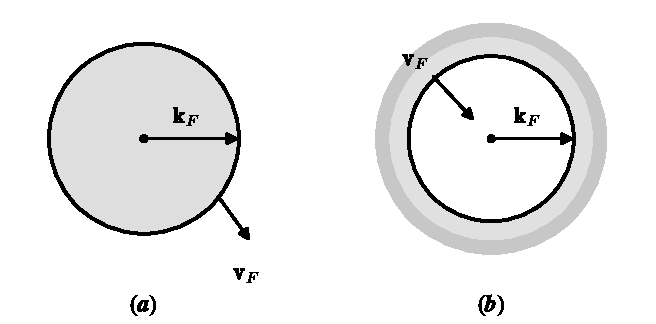
\includegraphics[width=0.72\textwidth]{fig_134.pdf}
\caption*{图 134\quad (a)“电子”球：$m^{*}$ 为正。(b)“空穴”球：$m^{*}$ 为负。}
\end{figure}

但请注意，假如我们有的一个 \emph{空穴球}（sphere of holes），我们就应当预期 $e$ 为正，也就是说，Hall 场的符号将与电子情形下得到的相反。这与上面的论证是一致的。假如我们把围绕球心的\emph{电子} 费米面拿来处理，式 (7.150) 仍然成立，但 $m^{*}$ 为负，因为此时电子速度指向球心。这个量在式 (7.151) 中仍是负的；然而在式 (7.152) 中，分母里出现的将是 $|m^{*}|$，因为正如式 (7.23) 中那样，我们实际计算的是
\begin{equation*}
\frac{e^{2}}{12\pi^{3}\hbar}\int\tau v_{F}^{2}\,\frac{\mathrm{d}S_{F}}{|v_{F}|}=\frac{e^{2}\tau}{12\pi^{3}}\int\frac{k_{F}\,\mathrm{d}S_{F}}{|m^{*}|}.\tag{7.153}
\end{equation*}
于是，$R$ 中将含有因子 $|m^{*}|/m^{*}=-1$，电荷的表观符号便反了过来。

这些公式即使在半导体的单一载流子带中也并不严格成立，因为 $\tau(\mathcal{E})$ 在被占据的各态之间可以变化。因此，修正因子依赖于散射机制 (7.50) 与 (7.73) 对能量的依赖关系，但它通常离 1 不远。把式 (7.147) 与式 (7.34) 结合起来，就给出 Hall 迁移率（Hall mobility）
\begin{equation*}
\mu_{H}=|R|\,\sigma c\tag{7.154}
\end{equation*}
即样品中多数载流子的 Hall 迁移率；其电荷的符号由 $R$ 的符号给出。

Hall 效应以及其他电流磁效应（galvanomagnetic phenomena）的理论，显然在很大程度上依赖于 Bloch 定理以及电子态的倒格子描述。在无序系统中，$\mathbf{k}$ 不再是好的量子数，通过 Boltzmann 方程进行的推导立刻变得可疑，我们就得转向某种更基本的理论，例如 Kubo 公式 (7.15)。然而事实是，目前还没有任何精确的理论可以取代简单的“电子球”公式 (7.147)——人们观察到，即使在电子平均自由程只有原子间距量级的情形下，这个公式在液态金属（§7.5）中也符合得非常好。不过，在局域态之间发生跳跃导电（hopping conduction）的极端情形下，是否还能观察到 Hall 效应，是很值得怀疑的。

\section{双带模型：磁致电阻}

现在假设我们有两类载流子，比如说，电子和空穴。对其中每一类单独而言，我们得到的都是同样的方程 (7.144)：
\begin{equation*}
\mathbf{E}=\frac{1}{\sigma_{1}}\mathbf{J}_{1}+\beta_{1}\,\mathbf{H}\wedge\frac{1}{\sigma_{1}}\mathbf{J}_{1},\tag{7.155}
\end{equation*}
其中
\begin{equation*}
\beta_{1}=\frac{e\tau_{1}}{m_{1}c}\tag{7.156}
\end{equation*}
而 $\sigma_{1}$ 是与第一类载流子相联系的电导率，这类载流子对电流的贡献为 $\mathbf{J}_{1}$。
\begin{figure}[H]
\centering
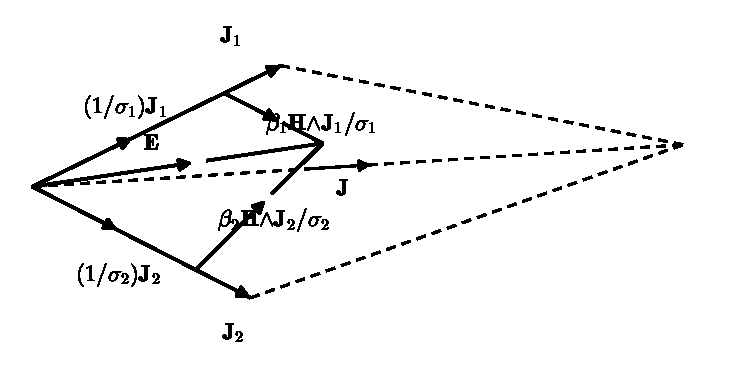
\includegraphics[width=0.72\textwidth]{fig_135.pdf}
\caption*{图 135\quad 来自两个载流子带的 Hall 效应贡献。}
\end{figure}
同样，对第二类载流子，
\begin{equation*}
\mathbf{E}=\frac{1}{\sigma_{2}}\mathbf{J}_{2}+\beta_{2}\,\mathbf{H}\wedge\frac{1}{\sigma_{2}}\mathbf{J}_{2}\tag{7.157}
\end{equation*}
表示它们的电流贡献与外加电场之间的关系。我们要求的是总电流
\begin{equation*}
\mathbf{J}=\mathbf{J}_{1}+\mathbf{J}_{2}.\tag{7.158}
\end{equation*}
对式 (7.155) 和 (7.157) 逐个使用形如式 (7.142) 的解，我们得到
\begin{equation*}
\mathbf{J}=\left(\frac{\sigma_{1}}{1+\beta_{1}^{2}H^{2}}+\frac{\sigma_{2}}{1+\beta_{2}^{2}H^{2}}\right)\mathbf{E}-\left(\frac{\sigma_{1}\beta_{1}}{1+\beta_{1}^{2}H^{2}}+\frac{\sigma_{2}\beta_{2}}{1+\beta_{2}^{2}H^{2}}\right)\mathbf{H}\wedge\mathbf{E},\tag{7.159}
\end{equation*}
这是一个相当复杂的公式\footnote{译注：原书式 (7.159) 第一括号中第二项的分母印作 $1+\beta_{2}^{2}H_{2}$，应为 $1+\beta_{2}^{2}H^{2}$。}，其几何表示见图 135。

要计算 Hall 系数，本应把这个公式反解出来，把 $\mathbf{E}$ 用 $\mathbf{J}$ 和 $\mathbf{H}\wedge\mathbf{J}$ 表出。但对弱的磁场，结果很容易得到：
\begin{align*}
R&=\frac{\sigma_{1}\beta_{1}+\sigma_{2}\beta_{2}}{(\sigma_{1}+\sigma_{2})^{2}}\\
&=\frac{\sigma_{1}^{2}R_{1}+\sigma_{2}^{2}R_{2}}{(\sigma_{1}+\sigma_{2})^{2}},\tag{7.160}
\end{align*}
其中 $R_{1}$ 和 $R_{2}$ 是相应的各类载流子单独存在时的 Hall 常数。这样，若 $R_{1}$ 与 $R_{2}$ 符号相反，我们看到的就是一个折中值。在半导体中，我们应当用相应载流子群的数目和迁移率来表出分电导率，即 $\sigma_{1}=n_{1}e\mu_{1}$，等等；这样一来，只有当某一类载流子明显占多数时，观测到的 Hall 迁移率 (7.154) 才会对应于某个确定的微观量。

磁致电阻则需要更细致的分析。我们要把 $\mathbf{J}$ 与 $\mathbf{E}$ 沿 $\mathbf{J}$ 方向的分量相比较。于是
\begin{align*}
\rho&=(\mathbf{J}\cdot\mathbf{E})/J^{2}\\
&=\frac{\dfrac{\sigma_{1}}{1+\beta_{1}^{2}H^{2}}+\dfrac{\sigma_{2}}{1+\beta_{2}^{2}H^{2}}}{\left(\dfrac{\sigma_{1}}{1+\beta_{1}^{2}H^{2}}+\dfrac{\sigma_{2}}{1+\beta_{2}^{2}H^{2}}\right)^{2}+\left(\dfrac{\sigma_{1}\beta_{1}H}{1+\beta_{1}^{2}H^{2}}+\dfrac{\sigma_{2}\beta_{2}H}{1+\beta_{2}^{2}H^{2}}\right)^{2}}.\tag{7.161}
\end{align*}
把它与没有磁场时的电阻
\begin{equation*}
\rho_{0}=\frac{1}{\sigma_{1}+\sigma_{2}}.\tag{7.162}
\end{equation*}
相比较，经过一点代数运算，就得到
\begin{equation*}
\frac{\Delta\rho}{\rho_{0}}\equiv\frac{\rho-\rho_{0}}{\rho_{0}}=\frac{\sigma_{1}\sigma_{2}(\beta_{1}-\beta_{2})^{2}H^{2}}{(\sigma_{1}+\sigma_{2})^{2}+H^{2}(\beta_{1}\sigma_{1}+\beta_{2}\sigma_{2})^{2}}.\tag{7.163}
\end{equation*}

这个公式本身并不十分重要；载流子能被当作分成两群、每群都具有如此简单性质的情形并不多见。尽管如此，它仍然展示了磁致电阻现象的主要特征。

首先，$\Delta\rho$ 本质上是正的，只有当 $\beta_{1}=\beta_{2}$ 时才为零。换句话说，当两群载流子在磁场中被偏转的量不同时——或者因为它们的质量不同、电荷不同，或者因为它们在被散射之前行经的距离不同——就不可能找到一个电场，使电流的这两个分量都保持沿同一方向行进。净电流作为各分量的矢量和，变小了；介质的表观电阻因而增大。

同样典型的是，$\Delta\rho$ 在弱场下正比于 $H^{2}$，但在强场下趋于\emph{饱和}（saturate）。不过后一效应与我们把载流子的能量面取为闭合曲面这一选择有关。正如我们在 §9.4 中将要看到的，有时可以找到一些特殊的晶向，使得 $\Delta\rho$ 并不饱和。

这类公式很容易推广到有许多不同类型载流子、各自分别对电流作出贡献的情形。换句话说，我们可以处理复杂的 费米面，其不同部分具有不同的 $\beta$ 值。因此，金属中磁致电阻的存在，就是 $\beta$ 在 费米面上多变——即有效质量取不同数值，或者也可能是 $\tau$ 有变化——的证据。但实际的公式是一个复杂的积分，其中含有 $\mathcal{E}(\mathbf{k})$ 在各处的各种局域导数，既不透明，也不便于用来从观测到的 $\Delta\rho$ 值推算 费米面的形状。

最简单的情形是半导体中载流子的一个“谷”（valley）（§6.6）；假如假定 $\tau$ 在每个能量面上为常数，这类载流子对电流磁效应的贡献可以相当容易地计算出来。式 (7.137) 中的 Lorentz 力算符显然是沿既垂直于 $\mathbf{v}$ 又垂直于 $\mathbf{H}$ 的方向取对 $\mathbf{k}$ 的导数。当电流沿谷轴方向时，形如式 (7.139) 的公式中的“Hall 质量”显然就是这个“横向”方向上的系数，比如说式 (6.44) 中的 $m_{i}$。但是，取不同取向的各个谷、连同逆质量张量 (6.48) 的各种非对角分量的贡献，
加起来，得到一个单一的 Hall 系数；假如晶体具有宏观立方对称性，这个系数必定是各向同性的。然而，这一对称性限制并不适用于磁致电阻：当晶体相对于电场和磁场的方向转动时，磁致电阻可以随之改变，从而给出关于半导体电子能带结构的重要信息。

上面的计算是针对\emph{横向磁致电阻}（transverse magneto-resistance）的——磁场垂直于电流方向。当磁场与载流导线平行时，还可以观察到\emph{纵向磁致电阻}（longitudinal magneto-resistance）。我们这个简单的双带模型不给出纵向磁致电阻，因为它假定每个能带都具有球对称性。纵向效应的公式要复杂得多，因为它们要求非球形的 费米面。在金属和半导体中也观察到这种效应。事实上，单晶样品电阻的改变，是电流方向和磁场方向相对晶体轴的取向的一个复杂函数。

在原理上不难、在实践上也并非不可能设想出其他依赖于环境磁场的输运“效应”。例如，热量沿温度梯度流动时，会产生一个类似于 Hall 效应的横向 \emph{Nernst 电场}（Nernst electric field）。按照晶体对称性对这些效应进行分类，并借助 Onsager 关系找出它们之间的相互联系，本身就是一项可观的理论研究；但只要弛豫时间近似成立，这些系数全都可以由 Boltzmann 方程导出。

关于式 (7.163)，还有一点值得注意。假设两群载流子具有相同的 $\tau$ 值，那么 $\Delta\rho/\rho_{0}$ 就只是 $\tau H$ 的函数。但此时 $\tau$ 本身将反比于电阻率 $\rho_{0}$，于是我们可以写出
\begin{equation*}
\frac{\Delta\rho}{\rho_{0}}=F\left(\frac{H}{\rho_{0}}\right),\tag{7.164}
\end{equation*}
其中 $F$ 是一个依赖于金属本身性质的函数。

这就是所谓的 \emph{Köhler 定则}（Köhler's rule）。它告诉我们：原则上，我们可以把不同样品的磁致电阻测量结果画在同一张基本图上；或者，利用在极低温度下 $\rho_{0}$ 很小的极纯样品，来研究超强磁场可能产生的效应。

但这条定则显然只是一个近似。两种不同类型的载流子具有相同的弛豫时间，或者甚至它们的弛豫时间之比保持不变——无论它们是被杂质还是被声子散射、在高温还是在低温——这些都绝不是必然的。这个定则所说的不过是：载流子的偏转正比于磁场与两次碰撞之间的时间的乘积。对 Köhler 定则的偏离，则表明不同类型的散射机制对不同群落的载流子有不同的影响。

 % 本文件由 scripts/assemble.py 自动装配，勿手改（改 parts/ 后重跑）
% 第8章 光学性质

\chapter{光学性质}

\epigraphbook{但是，轻些！那是什么光从那边的窗户透出来……}{Romeo and Juliet}

\section{宏观理论}

在本章中，我们讨论电磁波射入固体并在其中传播的问题。众所周知，有些固体是\emph{透明的}，另一些是\emph{不透明的}；有些固体表面\emph{强烈反射}，另一些则倾向于\emph{吸收}照射到其上的辐射。这些效应依赖于辐射的频率；因此我们把整个电磁波谱——从长波无线电波一直到软 X 射线——都包括进来。

电磁波是 Maxwell 方程组的解。我们把它写成如下形式
\begin{equation*}
\left.\begin{aligned}
\nabla\wedge\mathbf{H} &= \frac{\epsilon}{c}\,\frac{\partial\mathbf{E}}{\partial t} + \frac{4\pi\sigma}{c}\,\mathbf{E}, &\qquad \nabla\cdot\mathbf{E} &= 0,\\[4pt]
\nabla\wedge\mathbf{E} &= -\frac{\mu}{c}\,\frac{\partial\mathbf{H}}{\partial t}, &\qquad \nabla\cdot\mathbf{H} &= 0.
\end{aligned}\right\}\tag{8.1}
\end{equation*}
在本章中我们将不考虑任何磁效应：取 $\mu = 1$。

自由空间中的传播同固体中的传播这两者的差别，由两个系数表述——介电常数（dielectric constant）$\epsilon$ 和电导率 $\sigma$。前者给出因 $\mathbf{E}$ 随时间变化而引起的位移电流的大小；后者则是电场所产生的真实电流的一种量度。

从这些方程中消去磁场，得
\begin{equation*}
\nabla^2\mathbf{E} = \frac{\epsilon}{c^2}\,\frac{\partial^2\mathbf{E}}{\partial t^2} + \frac{4\pi\sigma}{c^2}\,\frac{\partial\mathbf{E}}{\partial t}\,.\tag{8.2}
\end{equation*}
这代表一个伴随耗散而传播的波。若选定频率 $\omega$，并写成
\begin{equation*}
\mathbf{E} = \mathbf{E}_0\exp\{i(\mathbf{K}\cdot\mathbf{r}-\omega t)\},\tag{8.3}
\end{equation*}
则波动方程要求
\begin{equation*}
-\mathbf{K}^2 = -\epsilon\,\frac{\omega^2}{c^2} - \frac{4\pi\sigma i\omega}{c^2}\,,\tag{8.4}
\end{equation*}
即
\begin{equation*}
K = \frac{\omega}{c}\left(\epsilon + \frac{4\pi\sigma i}{\omega}\right)^{\frac{1}{2}}.\tag{8.5}
\end{equation*}
这样，一般说来传播常数 $K$ 就是一个复数。而在自由空间中，我们应当简单地有
\begin{equation*}
K = \frac{\omega}{c},\tag{8.6}
\end{equation*}
正如一个以光速行进的波那样。在介质中，速度有所改变：我们说相速被一个\emph{复折射率}（complex refractive index）所除
\begin{equation*}
\mathsf{N} = \left(\epsilon + \frac{4\pi\sigma i}{\omega}\right)^{\frac{1}{2}}.\tag{8.7}
\end{equation*}
从宏观上观察到的光学性质的整个理论，都可以用 $\mathsf{N}$ 来表述。例如，设有一个频率为 $\omega$ 的扰动试图作为平面波沿 $z$ 方向传播，并设我们写出
\begin{equation*}
\mathsf{N} = \mathsf{n} + i\mathsf{k}\tag{8.8}
\end{equation*}
表示 $\mathsf{N}$ 的实部和虚部。于是传播常数变为
\begin{equation*}
K = \frac{\mathsf{n}\omega}{c} + \frac{i\mathsf{k}\omega}{c},\tag{8.9}
\end{equation*}
从而波 (8.3) 变为
\begin{equation*}
\mathbf{E} = \mathbf{E}_0\exp\left\{i\omega\left(\frac{\mathsf{n}z}{c} - t\right)\right\}\exp\left(-\frac{\mathsf{k}\omega z}{c}\right),\tag{8.10}
\end{equation*}
速度减小为 $c/\mathsf{n}$，而波在前进时受到\emph{阻尼}，每行进一个波长就衰减一个比例 $\exp(-2\pi\mathsf{k}/\mathsf{n})$。

波的这种阻尼当然与电磁能量的吸收相联系。为计算吸收，我们应当用 Maxwell 方程求出与 (8.10) 相伴随的电流。它就是 (8.1) 第一式的右端
\begin{equation*}
\begin{aligned}
\mathbf{J} &= \left(-\frac{i\omega\epsilon}{c} + \frac{4\pi\sigma}{c}\right)\mathbf{E}\\
&= -\frac{i\omega}{c}\,\mathsf{N}^2\mathbf{E}
\end{aligned}\tag{8.11}
\end{equation*}
依式 (8.7)。产生焦耳热的速率是下式的实部：
\begin{equation*}
\mathbf{J}\cdot\mathbf{E} = -\frac{i\omega}{c}\,\mathsf{N}^2 E^2.\tag{8.12}
\end{equation*}
于是，\emph{吸收系数}（absorption coefficient）——即每通过单位厚度材料所吸收的能量份额——由下式给出
\begin{equation*}
\eta = \frac{\mathrm{Re}(\mathbf{J}\cdot\mathbf{E})}{\mathsf{n}|\mathbf{E}|^2} = \frac{2\mathsf{k}\omega}{c}\,.\tag{8.13}
\end{equation*}
常被研究的另一种情形，是辐射入射到材料的平面表面上。一般说来，这是一个复杂的光学问题，但我们只需考虑
\begin{figure}[H]
\centering
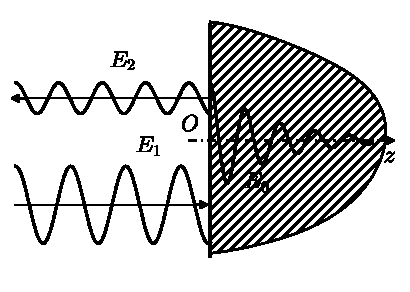
\includegraphics[width=0.72\textwidth]{fig_136.pdf}
\caption*{图 136\quad （原书此图无图注。）}
\end{figure}
垂直入射的情形。我们要构造 Maxwell 方程组的一个解，使其在介质内部具有 (8.10) 的形式，而在外部则与一个入射波和一个反射波相匹配。于是，对 $z > 0$ 我们写出
\begin{equation*}
E_x = E_0\exp\{i\omega(\mathsf{N}z/c - t)\},\tag{8.14}
\end{equation*}
而对于 $z < 0$，即在外部自由空间中，我们写出
\begin{equation*}
E_x = E_1\exp\{i\omega(z/c - t)\} + E_2\exp\{-i\omega(z/c + t)\},\tag{8.15}
\end{equation*}
分别对应于振幅为 $E_1$、向右行进的波和振幅为 $E_2$、向左行进的波。在边界上使二者匹配，得
\begin{equation*}
E_0 = E_1 + E_2.\tag{8.16}
\end{equation*}
但这些波还伴随有磁场，其磁矢量譬如说沿 $y$ 方向。用 Maxwell 方程组算出 $H_y$，得
\begin{equation*}
-\mathsf{N}E_0 = E_2 - E_1\tag{8.17}
\end{equation*}
此式是与外部的波相匹配而得到的。于是，反射波与入射波的复振幅之比为
\begin{equation*}
\frac{E_2}{E_1} = \frac{1-\mathsf{N}}{1+\mathsf{N}},\tag{8.18}
\end{equation*}
它对应于一个实的\emph{反射系数}（reflection coefficient）
\begin{equation*}
\mathsf{R} = \left|\frac{1-\mathsf{N}}{1+\mathsf{N}}\right|^2 = \frac{(\mathsf{n}-1)^2+\mathsf{k}^2}{(\mathsf{n}+1)^2+\mathsf{k}^2}\tag{8.19}
\end{equation*}
以复折射率 $\mathsf{N}$ 的实部和虚部即式 (8.8) 表出。

显然，对反射系数和吸收系数各作一次独立测量，便足以定出 $\mathsf{n}$ 和 $\mathsf{k}$ 的值。因此，它们就是人们通常引用的光学常数，其理论正是我们将在本章中讨论的。实际中的实验可能要复杂得多——例如相对表面成一定角度的反射，或穿过薄膜的透射——但从原则上讲，其结果都应当由这同样两个系数来描述。

然而，系数 $\mathsf{n}$ 和 $\mathsf{k}$ 并非彼此完全独立。它们由\emph{色散关系}（dispersion relations）联系起来。(8.11) 中的 $\mathsf{N}^2$ 这类量，就是\emph{广义极化率}（generalized susceptibility）$\alpha(\omega)$ 的一个例子，出现在如下关系中
\begin{equation*}
D(\omega) = \alpha(\omega)\,F(\omega)\tag{8.20}
\end{equation*}
它联系着广义的“位移” $D$ 与“力” $F$ 在某个频率 $\omega$ 处的 Fourier 分量。正如初等交流电路理论中那样，它必须是一个复量
\begin{equation*}
\alpha(\omega) = \alpha'(\omega) + i\alpha''(\omega)\tag{8.21}
\end{equation*}
以描述 $D$ 与 $F$ 之间的相位差。

但 (8.20) 只不过是
\begin{equation*}
D(t) = \int_{-\infty}^{\infty} A(t-t^{\prime})\,F(t^{\prime})\,dt^{\prime},\tag{8.22}
\end{equation*}
的 Fourier 变换；其中时刻 $t$ 的位移是系统对在所有其他时刻 $t^{\prime}$ 作用的力的\emph{线性响应}（linear response）的总和。但是在力施加\emph{之后}才可能有位移：响应函数受到\emph{因果性}（causality）这一严格条件的约束：
\begin{equation*}
A(t-t^{\prime}) \equiv 0 \qquad \text{当 } t^{\prime} > t \text{ 时}.\tag{8.23}
\end{equation*}
换言之，极化率的 Fourier 积分被完全确定为
\begin{equation*}
\alpha(\omega) = \int_{-\infty}^{\infty} A(t)\,e^{i\omega t}\,dt \equiv \int_0^{\infty} A(t)\,e^{i\omega t}\,dt.\tag{8.24}
\end{equation*}
其中不包含任何来自 $t$ 负值的贡献。

为赋予这类积分以意义，通常把 $\alpha(\omega)$ 当作\emph{复}变量 $\omega$ 的函数来处理，比如说让它带上一个无穷小的正虚部 $i\epsilon$。此外，(8.24) 的形式还意味着：这个函数在复 $\omega$ 平面上实轴上方没有奇点，并且在下半平面的所有方向上随 $|\omega|\to\infty$ 而趋于零。稍作一点泛函分析——把 Cauchy 定理应用于一条沿实轴行进、再经无穷大半圆返回的围道——便得到公式
\begin{equation*}
\alpha(\Omega) = \frac{1}{i\pi}\int_{-\infty}^{\infty}\frac{\alpha(\omega)}{\omega-\Omega}\,d\omega\tag{8.25}
\end{equation*}
其中积分取其主值，而频率变量为实数。

关于“负频率”的 Fourier 变换的定义意味着 $\alpha(-\omega)$ 是 $\alpha(\omega)$ 的复共轭。由 (8.25) 我们推出极化率 (8.21) 的实部与虚部之间的 \emph{Kramers--Kronig 关系}（Kramers--Kronig relations）
\begin{equation*}
\alpha'(\Omega) = \frac{2}{\pi}\int_0^{\infty}\frac{\omega\,\alpha''(\omega)\,d\omega}{\omega^2-\Omega^2} + \mathrm{const.},\tag{8.26}
\end{equation*}
以及
\begin{equation*}
\alpha''(\Omega) = -\frac{2\Omega}{\pi}\int_0^{\infty}\frac{\alpha'(\omega)\,d\omega}{\omega^2-\Omega^2}\,.\tag{8.27}
\end{equation*}
在我们这里的情形，$\mathsf{N}^2$ 的实部和虚部分别是
\begin{equation*}
\mathsf{N}^2 = (\mathsf{n}^2 - \mathsf{k}^2) + 2\mathsf{n}\mathsf{k}i,\tag{8.28}
\end{equation*}
于是我们得到如下条件
\begin{equation*}
\mathsf{n}^2(\omega) - \mathsf{k}^2(\omega) = \frac{2}{\pi}\int_0^{\infty}\frac{\omega'\,2\mathsf{n}(\omega^{\prime})\,\mathsf{k}(\omega^{\prime})\,d\omega^{\prime}}{\omega'^{2}-\omega^{2}} + \mathrm{const.},\tag{8.29}
\end{equation*}
以及
\begin{equation*}
2\mathsf{n}(\omega)\,\mathsf{k}(\omega) = -\frac{2\omega}{\pi}\int_0^{\infty}\frac{\left\{\mathsf{n}^2(\omega^{\prime}) - \mathsf{k}^2(\omega^{\prime})\right\}d\omega^{\prime}}{\omega'^{2}-\omega^{2}}\,.\tag{8.30}
\end{equation*}
由这些关系，假如我们比如说知道了吸收系数在所有频率上作为频率的函数，那么就能分别求出 $\mathsf{n}(\omega)$ 和 $\mathsf{k}(\omega)$。它们并不是某个特定模型的偶然结果；其证明仅仅依赖于因果性条件 (8.23)，是完全普遍的，适用于任何线性响应函数，例如介电函数（dielectric function）(5.16) 或表面阻抗 (8.106)。

\section{色散与吸收}

固体的最简单模型，是一组固定不动的、彼此独立的中性原子。电磁波对这样的系统会有什么影响？倘若读者对这一理论不太熟悉，我们就在一个简单的例子中把它勾画出来：设每个原子只含一个电子，该电子处于基态轨道 $\phi_0(\mathbf{r})$ 中，可以被激发到较高的轨道 $\phi_j(\mathbf{r})$。

设波中原子附近的电场由下式给出
\begin{equation*}
\mathbf{E}(t) = \mathbf{E}_x\left(e^{i\omega t} + e^{-i\omega t}\right),\tag{8.31}
\end{equation*}
其中忽略了随距离的变化，正如 (8.3) 中那样。我们采用含时微扰论，并设电子波函数在任一特定时刻可以写成
\begin{equation*}
\psi(\mathbf{r},t) = \phi_0\exp(-i\mathcal{E}_0 t/\hbar) + \sum_j c_j(t)\,\phi_j\exp(-i\mathcal{E}_j t/\hbar).\tag{8.32}
\end{equation*}
我们把 $e\mathbf{E}\cdot\mathbf{r}$ 当作作用在电子上的微扰势。把 (8.32) 代入含时 Schrödinger 方程，用 $\phi_j^{*}$ 乘遍各项再积分（译注：原文为“用 $\phi_0$ 相乘”，按式 (8.33) 应为 $\phi_j^{*}$），容易证明：较高态的系数必须近似满足微分方程
\begin{equation*}
i\hbar\frac{dc_j}{dt} = \int \phi_j^{*}\,e\mathbf{E}(t)\cdot\mathbf{r}\,\phi_0\,d\mathbf{r}\,e^{i(\mathcal{E}_j-\mathcal{E}_0)t/\hbar}\tag{8.33}
\end{equation*}
它有解
\begin{align*}
c_j(t) &= \frac{1}{i\hbar}\int_0^t e\mathbf{E}_x\,x_{j0}\left(e^{i\omega t}+e^{-i\omega t}\right)e^{i(\mathcal{E}_j-\mathcal{E}_0)t/\hbar}\\
&= e\mathbf{E}_x\,x_{j0}\left\{\frac{1-e^{i(\hbar\omega+\mathcal{E}_j-\mathcal{E}_0)t/\hbar}}{\hbar\omega+(\mathcal{E}_j-\mathcal{E}_0)} - \frac{1-e^{i(-\hbar\omega+\mathcal{E}_j-\mathcal{E}_0)t/\hbar}}{\hbar\omega-(\mathcal{E}_j-\mathcal{E}_0)}\right\},\tag{8.34}
\end{align*}
其中
\begin{equation*}
e\,x_{j0} \equiv \int \phi_j^{*}\,e\,x\,\phi_0\,d\mathbf{r},\tag{8.35}
\end{equation*}
也就是说，它是电子的电偶极矩沿场的电矢量方向、在态 $\phi_0$ 与 $\phi_j$ 之间的矩阵元。

现在，量子理论书中的通常做法是研究 $|c_j(t)|^2$，并证明：除了满足条件
\begin{equation*}
\hbar\omega = \hbar\omega_j \equiv (\mathcal{E}_j - \mathcal{E}_0).\tag{8.36}
\end{equation*}
的那些 $\omega$ 值之外，它都剧烈振荡。于是人们证明，将会发生一次从态 $\phi_0$ 到态 $\phi_j$ 的量子跃迁，其概率由矩阵元 (8.35) 的平方决定。

但现在我们改走另一条路：计算原子在这个含时态中的偶极矩之值。由 (8.32) 和 (8.34) 我们得到
\begin{align*}
\langle ex(t)\rangle &= \int \psi^{*}(\mathbf{r},t)\,ex\,\psi(\mathbf{r},t)\,d\mathbf{r}\\
&= \sum_j \left\{ex_{0j}\,c_j(t)\,e^{-i\omega_j t} + ex_{j0}\,c_j^{*}(t)\,e^{i\omega_j t}\right\}\\
&= \mathbf{E}_x\sum_j e^2\,|x_{0j}|^2\,\frac{1}{\hbar}\left\{\frac{1}{\omega_j-\omega}+\frac{1}{\omega_j+\omega}\right\}\left(e^{i\omega t}+e^{-i\omega t}\right)\tag{8.37}
\end{align*}
以及一些振荡迅速、与应用场不同相的项。

这样，原子的偶极矩正比于场。我们说\emph{原子极化率}（atomic polarizability）由下式给出
\begin{equation*}
\alpha(\omega) = \sum_j \frac{e^2|x_{0j}|^2}{\hbar}\,\frac{2\omega_j}{\omega_j^2-\omega^2}\,.\tag{8.38}
\end{equation*}
为讨论这类表达式的数量级，我们可以利用 Thomas--Reiche--Kuhn 求和规则——它是 (5.48) 的一个较简单的特例。这个规则是
\begin{equation*}
\frac{2m}{\hbar^2}\sum_j \hbar\omega_j\,|x_{0j}|^2 = 1\,;\tag{8.39}
\end{equation*}
为方便起见，定义第 $j$ 个跃迁的\emph{振子强度}（oscillator strength）
\begin{equation*}
f_j = \frac{2m}{\hbar^2}\,\hbar\omega_j\,|x_{0j}|^2,\tag{8.40}
\end{equation*}
并把 (8.38) 写成如下形式
\begin{equation*}
\alpha(\omega) = \frac{e^2}{m}\sum_j \frac{f_j}{\omega_j^2-\omega^2},\tag{8.41}
\end{equation*}
其中各个数 $f_j$ 在所有跃迁上相加为一。

现在，若把 $N$ 个这样的原子聚拢到每单位体积中，我们就得到一种介质，其介电常数有一个实部
\begin{align*}
\epsilon(\omega) &= 1 + 4\pi N\alpha(\omega)\\
&= 1 + \frac{4\pi N e^2}{m}\sum_j \frac{f_j}{\omega_j^2-\omega^2}\,.\tag{8.42}
\end{align*}
严格说来，我们应当把这个\emph{横}（transverse）介电常数，与第 5 章中讨论过的静电场的\emph{纵}（longitudinally）偏振波的介电常数区分开来。不过在长波极限下——即对通常的“光学”现象——这两个量是相同的，因为屏蔽或原子极化效应相对地说是局域的，并且主要依赖于每个离子或原子紧邻区域中电场的强度。
这是色散公式的原型。有趣的是，它恰好可以归结为 \S 5.7 中已经讨论过的情形。如果电子是“自由的”——也就是说，所有 $\omega_j$ 均为零，而各个 $f_j$ 之和为一——我们便可以像 (5.53) 那样写出
\begin{equation*}
\omega_p^2 = \frac{4\pi N e^2}{m}\tag{8.43}
\end{equation*}
来为我们这个每单位体积 $N$ 个电子的系统定义等离体频率（plasma frequency）；于是 (8.42) 就复现了 (5.67)，即导致紫外透明性现象的公式。然而要注意，横向光子实际上几乎不能直接激发纵向等离激元（plasmon）。要观察\emph{等离激元谱线}（plasmon lines），需要用高能电子去激发电子气，或者透过薄膜去观察，在后一种情形中可以观察到\emph{表面等离激元模}（surface plasmon modes）。

但在一般情况下，$\omega_j$ 的最低值应对应于光学或红外频率，$\epsilon$ 随 $\omega$ 的变化要更复杂一些。在低频下，我们可能得到静态介电常数
\begin{equation*}
\epsilon(0) = 1 + \sum_j f_j\,\frac{\omega_p^2}{\omega_j^2},\tag{8.44}
\end{equation*}
它明显大于 1。但 $\epsilon(0)$ 不会非常大，因为对大多数固体来说，$\omega_p$ 与自由原子的普通光学频率大致相当。

接着，随着 $\omega$ 增大，$\epsilon(\omega)$ 增大，直到在 $\omega = \omega_j$ 处出现一个奇点。此后，$\epsilon(\omega)$ 在某段频率范围内变为负值，直到靠近下一个共振频率时才重新变正。不过最终，$\epsilon(\omega)$ 将趋于公式 (5.67)：
\begin{equation*}
\epsilon(\omega) \to 1 - \frac{\omega_p^2}{\omega^2},\tag{8.45}
\end{equation*}
条件是 $\omega$ 大于所有 $\omega_j$。

在每一个 $\omega_j$ 附近，我们都有一段\emph{反常色散}（anomalous dispersion）区。特别地，若 $\epsilon$ 为负，则由 (8.7)，折射率 $\mathsf{N}$ 变为纯虚数；于是
\begin{equation*}
\mathsf{n} = 0,\quad \mathsf{k} = |\epsilon|^{\frac{1}{2}},\tag{8.46}
\end{equation*}
从而由 (8.19)，光将被固体表面\emph{完全反射}（total reflection）。实际上，晶体看起来会一直保持透明——尽管折射率非常高——直到 $\omega = \omega_j$ 处突然变得不透明且完全反射，然后在更高的频率上重新变为透明。

但这与我们的色散关系 (8.29) 和 (8.30) 不相容。还必须存在某种吸收，其量度是乘积 $2\mathsf{n}\mathsf{k}\omega$。的确，这正是我们在含时微扰处理中暂且搁置的那一方面——与原子跃迁 (8.36) 相联系的吸收。它作为频率 $\omega_j$ 处的一条锐线出现——想必是一个 delta 函数。为了满足色散关系 (8.29) 并在 (8.42) 中给出正确的色散项，我们必须有
\begin{equation*}
2\omega\,\mathsf{n}(\omega)\,\mathsf{k}(\omega) = \frac{\pi}{2}\,\frac{4\pi N e^2}{m}\sum_j f_j\,\delta(\omega-\omega_j);\tag{8.47}
\end{equation*}
\begin{figure}[H]
\centering
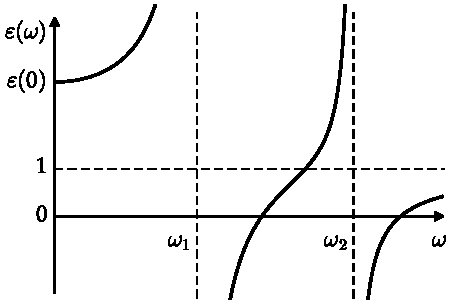
\includegraphics[width=0.72\textwidth]{fig_137.pdf}
\caption*{图 137\quad 光的色散。}
\end{figure}
这必定是复介电常数的虚部，后者取如下形式
\begin{equation*}
\epsilon(\omega) = 1 + \frac{4\pi N e^2}{m}\sum_j f_j\left\{\frac{1}{\omega_j^2-\omega^2} + \frac{i\pi}{2\omega}\,\delta(\omega^2-\omega_j^2)\right\}.\tag{8.48}
\end{equation*}
$\omega_j$ 附近的大折射率在这个频率上变成一条尖锐的吸收线。

实际上，我们永远不会看到一条无限锐的谱线。总会有某种展宽，来自杂质等因素，或者仅仅来自能级的自然辐射弛豫。正如标准量子理论所表明的，这类效应可以在分析中以唯象方式纳入：比如说在 (8.34) 中插入一个衰减因子 $\exp(-\frac{1}{2}\Gamma t)$，它对应于（振幅\emph{平方}的）量级为 $1/\Gamma$ 秒的衰减时间。

在代数推导中很容易追踪这样一个因子的作用：它相当于
\begin{figure}[H]
\centering
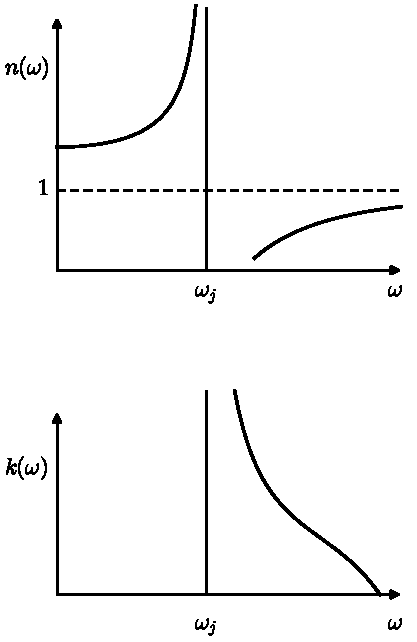
\includegraphics[width=0.72\textwidth]{fig_138.pdf}
\caption*{图 138\quad 折射率的实部和虚部。}
\end{figure}
\begin{figure}[H]
\centering
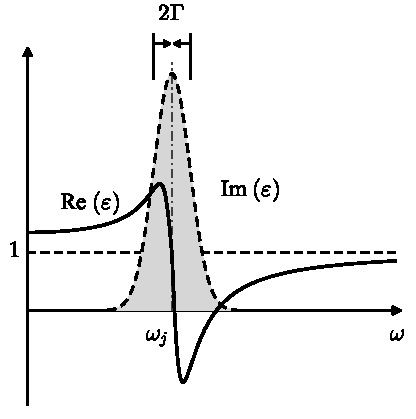
\includegraphics[width=0.72\textwidth]{fig_139.pdf}
\caption*{图 139\quad 色散曲线的展宽。}
\end{figure}
在 (8.37) 或 (8.38) 的 $\omega_j$ 上加一个 $\frac{1}{2}i\Gamma$。如果相对于 $\omega_j^2$ 略去 $\Gamma^2$，那么对于极化率的实部——从而也就是 $\epsilon(\omega)$ 的实部——我们会得到如下类型的项
\begin{equation*}
f_j\,\frac{\omega_j^2-\omega^2}{(\omega_j^2-\omega^2)^2+\omega^2\Gamma^2}\tag{8.49}
\end{equation*}
用以取代 $f_j/(\omega_j^2-\omega^2)$。这起到了消除 $\mathsf{n}$ 中奇点的作用，
并把色散函数在频率上铺展开来，形成宽度约为 $2\Gamma$ 的一段范围。

众所周知，弛豫对吸收线本身的影响，是把 delta 函数铺展成一个有限大小的函数，在 $\omega = \omega_j$ 附近其形式为
\begin{equation*}
\frac{\Gamma/2\pi}{(\omega_j-\omega)^2+\frac{1}{4}\Gamma^2} \approx \frac{2\Gamma\omega^2/\pi}{(\omega_j^2-\omega^2)^2+\Gamma^2\omega^2}\tag{8.50}
\end{equation*}
\begin{figure}[H]
\centering
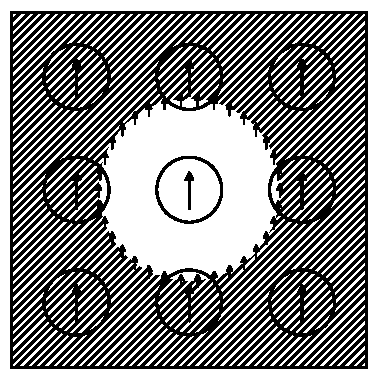
\includegraphics[width=0.72\textwidth]{fig_140.pdf}
\caption*{图 140\quad Lorentz 修正：用均匀极化介质中一个球形空腔的场，取代相邻原子上的偶极子在原子处产生的局域场。}
\end{figure}
实际上，(8.49) 与 (8.50) 可以合并成一个类似 (8.48) 的公式
\begin{align*}
\epsilon(\omega) &= 1 + \frac{4\pi N e^2}{m}\sum_j f_j\left\{\frac{\omega_j^2-\omega^2}{(\omega_j^2-\omega^2)^2+\omega^2\Gamma_j^2} + \frac{i\Gamma_j\omega}{(\omega_j^2-\omega^2)^2+\omega^2\Gamma_j^2}\right\}\\
&= 1 + \frac{4\pi N e^2}{m}\sum_j \frac{f_j}{(\omega_j^2-\omega^2)-i\omega\Gamma_j},\tag{8.51}
\end{align*}
它差不多就是最一般类型的色散公式。虽然它是针对独立原子模型算出的，却为任何吸收谱由一系列分立谱线组成的系统提供了一个唯象表达式。

在这个分析中，还应作一个进一步的修正。关系 (8.42) 意味着极化每个原子的\emph{局域}场（local field）与施加于晶体的\emph{宏观}场（macroscopic field）相同。严格说来这并不成立；原子并非处于一种绝对连续的
%JOIN%
介质，而是占据格子中的一个格点；在那里，它被“其他”同样极化了的原子所包围，却并不被它们贯穿（见 §2.3）。众所周知，在初等静电学和静磁学中，局域场必须有一个修正；如果包围原子的“空腔”多少近似球形，那么我们就得到局域场的 \emph{Lorentz 修正}（Lorentz correction）
\begin{equation*}
\mathbf{E}_{\mathrm{local}} = \mathbf{E}_{\mathrm{macroscopic}} + \frac{4}{3}\pi\mathbf{P},\tag{8.52}
\end{equation*}
其中 $\mathbf{P}$ 是平均极化。这就导致 \emph{Clausius–Mosotti 关系}（Clausius–Mosotti relation）
\begin{equation*}
\left(\frac{\epsilon-1}{\epsilon+2}\right) = \frac{4}{3}\pi N\alpha\tag{8.53}
\end{equation*}
以取代 (8.42)。结果是，观测到的介电常数和折射率将遵循一个比 (8.51) 更复杂的公式；例如，“完全”反射的频段就可能得以避免。

当介电极化是由于液体或固体分子上\emph{永久}偶极矩（permanent dipole moments）的排齐所致时，我们必须引入进一步的修正，例如 \emph{Onsager 局域场}（Onsager local field）模型，它把邻近原子矩取向的涨落考虑了进去。

\section{离子晶体中的光学模}

让我们回到格子的运动方程，如 §2.1 中那样。那里已经证明，第 $l$ 个晶胞中格点 $s$ 上的离子，其位移满足 (2.7)，即
\begin{equation*}
M_s \ddot{\mathbf{u}}_{sl} = -\sum_{s'\boldsymbol{h}} \mathsf{G}_{ss'}(\boldsymbol{h})\cdot\mathbf{u}_{s',\,l+\boldsymbol{h}}.\tag{8.54}
\end{equation*}
现在假设我们用形如 (8.3) 的电磁波来驱动这个系统。必须在 (8.54) 的右端加上一个力
\begin{equation*}
\boldsymbol{e}_s\,\mathbf{E}_0\exp\{i(\mathbf{K}\cdot\boldsymbol{l}-\omega t)\},\tag{8.55}
\end{equation*}
其中 $\boldsymbol{e}_s$ 是晶胞中格点 $s$ 上的离子所带的电荷。

要处理这样的非齐次项，我们只需要微分方程 (8.54) 的一个特解。显然，采用 (2.8) 的假设并令 $\boldsymbol{q}=\mathbf{K}$，随空间变化的因子即被消去；我们便得到波矢为 $\mathbf{K}$ 的模的振幅 $\mathbf{U}_{s\mathbf{K}}$ 所满足的方程
\begin{equation*}
M_s \ddot{\mathbf{U}}_{s\mathbf{K}} = -\sum \mathsf{G}_{ss'}(\mathbf{K})\cdot\mathbf{U}_{s'\mathbf{K}} + \boldsymbol{e}_s\,\mathbf{E}_0\,e^{-i\omega t}.\tag{8.56}
\end{equation*}
要看出这些方程之解的形式，让我们考虑 (2.22) 中那个双原子线性链的简单模型。实际上，我们所考虑的电磁波在原子的尺度上波长非常之大，
因此可以取 $\cos Ka \approx 1$。如果两个原子带有异号电荷——在典型的离子晶体中情形正是如此——那么我们就有
\begin{equation*}
\left.
\begin{aligned}
M_1 \ddot{U}_1 &= 2\alpha(U_2-U_1) + \boldsymbol{e}E_0\,e^{-i\omega t},\\
M_2 \ddot{U}_2 &= 2\alpha(U_1-U_2) - \boldsymbol{e}E_0\,e^{-i\omega t}.
\end{aligned}
\right\}
\tag{8.57}
\end{equation*}
这两个方程有解
\begin{equation*}
(U_1-U_2) = \frac{\boldsymbol{e}E_0(1/M_1+1/M_2)}{\omega_T^2-\omega^2}\,e^{-i\omega t},\tag{8.58}
\end{equation*}
其中 $\omega_T$ 是系统在 $\boldsymbol{q}=0$ 处的固有频率，即由 (2.25) 给出的值。我们可以算出与这种运动相联系的偶极矩，并把它表示成晶格的一个极化率
\begin{equation*}
4\pi N\alpha(\omega) = \frac{4\pi N\boldsymbol{e}^2(1/M_1+1/M_2)}{\omega_T^2-\omega^2}.\tag{8.59}
\end{equation*}
于是，一个纯粹经典的论证就把我们引到了一个类似于 (8.42) 的色散公式。(8.59) 的分子可以写成 $\Omega_p^{\prime 2}$，表明它非常像离子集合体的等离体频率 (6.81)。由于离子比电子重得多，它必定远小于 $\omega_p^2$。另一方面，$\omega_T$ 正是长波长晶格振动的频率，比原子或离子中任何电子跃迁的能量都小得多。因此，在很宽的频率范围内，我们可以写成
\begin{equation*}
\epsilon(\omega) \approx \epsilon(\infty) + \frac{\Omega_p^{\prime 2}}{\omega_T^2-\omega^2},\tag{8.60}
\end{equation*}
其中误差来自 (8.53) 那样的局域场效应。在这个公式中，$\epsilon(\infty)$ 表示在 $\omega \gg \omega_T$（即电子跃迁尚未被激发之前）由折射率的观测推出的介电常数。由此我们可以导出静态介电常数的 \emph{Born 方程}（Born equation）
\begin{equation*}
\epsilon(0) \approx \epsilon(\infty) + \Omega_p^{\prime 2}/\omega_T^2.\tag{8.61}
\end{equation*}
在三维离子晶体中，$\omega_T$ 将是一个\emph{横向}极化的光学支的频率，其偶极矩与横向电磁波强烈地相互作用。实际上，我们这里得到的是一个\emph{极化激元}（polariton）——光与晶体极化的一种混合模，它才是材料中真正的传播模。当 $\omega$ 扫过 $\omega_T$ 时，介电常数变为负值：正如 (5.67) 和 (8.46) 的情形，辐射将被晶体表面完全反射。\emph{剩余射线效应}（Reststrahlen effect）——晶体中电磁传播的一个禁区——将一直持续到譬如说 $\omega_L$ 处，在该处 (8.60) 重新变为正，即
\begin{equation*}
\omega_L^2 = \omega_T^2 + \Omega_p^{\prime 2}/\epsilon(\infty).\tag{8.62}
\end{equation*}
但介电常数的定义意味着（参见 (5.59)）：在这个频率上，无需任何外部激发，晶体内部就可以存在非常大的电场变化。这正是离子晶格中等离体振荡的类比，其中既有局域原子间力的贡献，也有长程静电场的贡献：$\omega_L$ 就是晶格谱中\emph{纵向}光学支的长波极限。由 (8.61) 和 (8.62) 我们得到与 (8.60) 相配的一个关系——\emph{Lyddane–Sachs–Teller 关系}（Lyddane–Sachs–Teller relation）
\begin{equation*}
\omega_L^2/\omega_T^2 = \epsilon(0)/\epsilon(\infty)\tag{8.63}
\end{equation*}
它对任何极性材料都相当普遍地成立。

实际上，(8.59) 和 (8.60) 的分母中应当含有一个虚项（参见 (8.51)），对应于耗散效应。例如，通过产生声子，电磁场的能量可能被吸收，而这些声子将通过力常数的非谐性（anharmonicity）与光学支相联系（§§2.11, 7.10, 8.4）。这类效应将是依赖于温度的，并且也应能被观察到，表现为谐和近似 (2.25) 或 (8.53) 中有效力常数 $\alpha$ 的变化。甚至还可能出现这样的情况：对某一组晶格位移而言，原子间力的平衡如此精妙，以致这种温度依赖使 $\omega_T^2$ 在某个临界温度 $T_c$ 以下取负值——这个事件我们在宏观上应当认作是向\emph{铁电相}（ferro-electric phase）的转变（§10.5），晶格结构从此带有永久的、内建的介电极化。

纵向光学支的频率比较低，这一点在\emph{极化子}（polaron）理论中很重要。离子晶体中的一个电子携带着静电场，使其周围的晶格极化。对于静止的电子，我们本可以用介电常数 $\epsilon(0)$；但晶格对运动电子的响应在动力学上受频率 $\omega_L$ 的限制，它描写介质介电极化的固有振荡。

这种情形与等离激元理论（§5.8）中的情形非常相似。如果电子的能量超过 $\hbar\omega_L$，就会产生一个光学声子，电子将被减速并受到强烈散射。即使电子运动得很慢，我们也必须考虑光学模中量子的虚激发与再吸收；
换言之，电子的行为就像一个被一团虚声子云包围着的粒子。这个复合客体的自能是速度的函数，因而载流子的有效“质量”会显著增大。

\emph{大极化子}（large polaron）的理想化哈密顿量，作为一个强相互作用的场论系统的模型，已被广泛研究过，但它在实践中并不是一个容易观察的对象。这个模型本身只在极化区域比晶格的一个晶胞多少大一些的时候才有效；否则，更合适的是自陷的\emph{小极化子}（small polaron）模型（§6.7）。

\section{光子–声子跃迁}

用场论的语言来说，晶体对红外的吸收被描写为一个\emph{光子}（photon）与一个或多个声子的相互作用。这类过程的选择定则，已经在 §§2.7、2.8 中以\emph{非弹性衍射}（inelastic diffraction）的名义导出过。例如在最简单的情形，衍射束波矢的\emph{改变}必须等于所发射声子的波矢，即
\begin{equation*}
\mathbf{k}-\mathbf{k}' = \mathbf{q}\tag{8.64}
\end{equation*}
同时辐射频率的改变必须等于声子的频率，
\begin{equation*}
\omega-\omega' = \nu\tag{8.65}
\end{equation*}
如 (2.101) 和 (2.102) 中那样。在某些特殊情形下，可以满足这些条件而不产生任何出射的衍射波；光子的全部能量和动量都转移给了晶体。

这里要注意的要点是，我们处理的是可见和红外波段的光，其波长比晶体的晶格常数大得多。因此，$|\mathbf{k}-\mathbf{k}'|$ 在布里渊区的尺度上必定极其微小。对于一切寻常的光学现象，我们可以取 $\mathbf{k}-\mathbf{k}'\approx 0$，而把注意力集中在区图式所允许的能量改变上；这一方面恰好与适用于 X 射线和中子的“衍射”观点互为补充——在后者中，动量的改变很大，但能量差却不容易探测。

我们这里考虑的过程，即一个光学声子的吸收或发射，因而在简约区图式中由 $\mathbf{q}=0$ 处一条近乎竖直的线来表示。如果光学频谱有好几个分支，那么原则上应当能观察到好几条不同的谱线，如图 141(b) 那样。但是这类过程的
强度将取决于电磁波与晶体耦合的矩阵元。正如 §8.3 中所见，对于大多数极性晶体的横向光学支，这种耦合强到如此程度，以致用弱相互作用的光子和声子来描述已不恰当，我们得到的将是剩余射线效应。但在某些化合物半导体中，可以找到偶极矩非常弱的光学支，在透过薄膜的透射光中能够观察到\emph{单声子吸收}（one-phonon absorption）。

\begin{figure}[H]
\centering
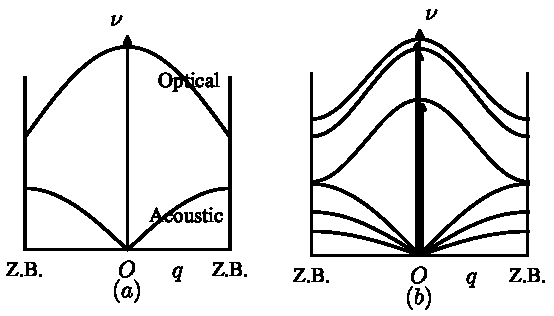
\includegraphics[width=0.72\textwidth]{fig_141.pdf}
\caption*{图 141\quad 光学模的吸收：(a) 一维图式；(b) 三维图式。}
\end{figure}

观察到光子的吸收（和发射）过程在布里渊区中是“竖直”的，这提示我们还可能有别的“竖直”跃迁，如图 142 所示。这是一个涉及一个声学支和一个光学支的跃迁。被吸收的光子，其能量显然由下式构成
\begin{equation*}
\hbar\omega = \hbar\nu_{\mathrm{optical}} - \hbar\nu_{\mathrm{acoustic}}.\tag{8.66}
\end{equation*}
实际上就是：一个光子和一个声学声子消失了；一个光学声子产生了。动量条件也同样得到满足。我们可以忽略光子的动量，简单地断言
\begin{equation*}
\hbar\mathbf{q}_{\mathrm{optical}} = \hbar\mathbf{q}_{\mathrm{acoustic}},\tag{8.67}
\end{equation*}
这正是“跃迁必须竖直”这句话所蕴含的意思。

\begin{figure}[H]
\centering
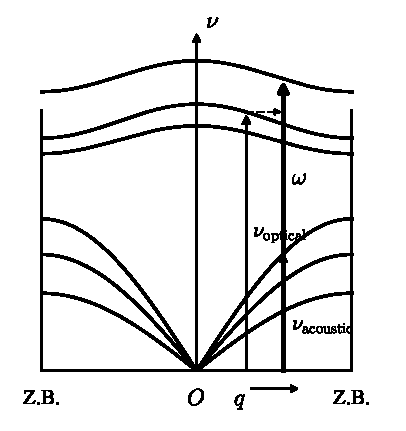
\includegraphics[width=0.72\textwidth]{fig_142.pdf}
\caption*{图 142\quad 多声子吸收。}
\end{figure}

这类过程为选择定则所允许，因此可以观察到。它们在远红外区给出整段整段的吸收带。这种吸收带的宽度和总体结构，显然
取决于从声学支到光学支可能发生的跃迁的种类及其间距。对这类过程作完整的讨论显然相当复杂，因为我们处理的是两个函数之差，而其中每一个函数都是布里渊区中 $\mathbf{q}$ 的函数。

这还没有穷尽一切可能的过程。我们可以把上述跃迁称为“差式”（difference）过程。同样还可能有\emph{求和带}（summation bands），其中由光子的能量产生\emph{两个}声子，但它们的动量大小相等、方向相反。在那种情形下
\begin{equation*}
\hbar\omega = \hbar\nu_{\mathrm{optical}} + \hbar\nu_{\mathrm{acoustic}},\tag{8.68}
\end{equation*}
并有
\begin{equation*}
\hbar\mathbf{q}_{\mathrm{optical}} = -\hbar\mathbf{q}_{\mathrm{acoustic}}.
\end{equation*}
要真正计算跃迁概率，我们需要知道偶极矩作为晶格位移的函数中的非线性项。例如，我们需要在如下表达式中的张量 $\mathbf{B}_{ss'}$
\begin{equation*}
\mathbf{M}_l = \sum_s \mathbf{A}_s\cdot\mathbf{u}_{sl} + \sum_{ss'} \mathbf{u}_{sl}\cdot\mathbf{B}_{ss'}\cdot\mathbf{u}_{s'l}\tag{8.69}
\end{equation*}
它给出第 $l$ 个晶胞中由位移 $\mathbf{u}_{sl}$ 产生的偶极矩。于是我们用 (2.8)、(2.10) 和 (2.129) 把每一位移用谱的各个分支的声子的湮没和产生算符表出。$\mathbf{B}_{ss'}$ 项对应于两个此类算符的乘积，它给出我们所寻求的双声子过程。跃迁的实际概率将包含如下形式的两个矩阵元的平方
\begin{equation*}
\left.
\begin{gathered}
\langle n_{\mathbf{q}}+1|a_{\mathbf{q}}^{*}|n_{\mathbf{q}}\rangle = (n_{\mathbf{q}}+1)^{\frac{1}{2}},\\
\text{或}\quad \langle n_{\mathbf{q}}-1|a_{\mathbf{q}}|n_{\mathbf{q}}\rangle = n_{\mathbf{q}}^{\frac{1}{2}},
\end{gathered}
\right\}
\tag{8.70}
\end{equation*}
对应于声子态的占据数增加或减少一个量子。由于 $n_{\mathbf{q}}$ 的平均值是温度的函数（如 (2.46) 那样），这些过程将是依赖于温度的。不过一般说来，非线性系数 $\mathbf{B}_{ss'}$ 很小，所以与单声子过程相比，这些带是弱的。

值得指出的是，对于任何一个分支，函数 $\nu_{\mathbf{q}}$ 都是 $\mathbf{q}$ 的连续周期函数，其周期为倒格子的周期（参见 §2.2）。由此可知，任何一对这类函数的和或差也具有同样的性质。于是，van Hove 定理（§2.5）适用于频率的分布；在观测谱中只可能出现图 27 所示的那四种类型的奇点（除非矩阵元引入额外的奇点）。

在式 (8.64)、(8.65) 中，我们写下了光作非弹性衍射的选择定则——即一个光子 $|\mathbf{k},\omega\rangle$ 变换为另一个光子 $|\mathbf{k}',\omega'\rangle$ 并发射一个声子 $|\mathbf{q},\nu\rangle$。这将表现为晶体所散射的一部分光的频移。这种一阶 Raman 效应显然等价于单声子吸收。晶体的二阶 Raman 谱含有来自双声子过程的谱带——如此等等。当涉及有限波矢的声学支时，我们称之为 Brillouin 散射。

动量选择定则 (8.64)、(8.67)、(8.68) 依赖于 Bloch 定理（见 §2.7）。若不存在完整的晶格平移对称性，跃迁便可以被允许到布里渊区中的任何一点。因此，晶格中的杂质或其他不完整性会诱发本来被禁止的红外吸收及类似的光学现象。这类效应的详细计算显然非常复杂，但由此可以直接观察到来自局域模（localized modes）的锐线以及来自共振（§2.12）的峰。

\section{带间跃迁}

当电子处于 Bloch 态、形成宽的能带时，电子从满态到空态的跃迁产生宽的吸收带。再者，对于光频，$\mathbf{K}$ 在布里渊区的尺度上很小，因此可以忽略光子的波矢，并假定所有跃迁都是“竖直的”（vertical），如图 143 所示。

\begin{figure}[H]
\centering
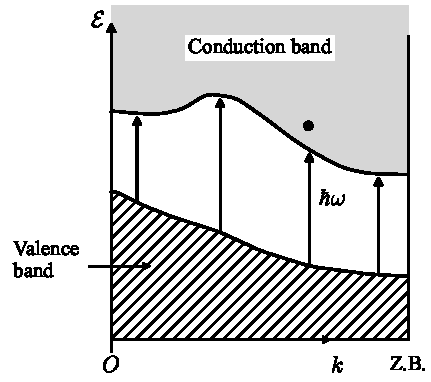
\includegraphics[width=0.72\textwidth]{fig_143.pdf}
\caption*{图 143\quad 半导体中的竖直带间跃迁。}
\end{figure}

我们已经在式 (5.45) 中写下了半导体介电常数的公式。在那里我们更关心的是所有波长下的静态行为；而现在我们关心的是 $\epsilon(\mathbf{q},\omega)$ 在长波极限下的频率依赖。由式 (5.57) 我们有

\begin{align*}
\epsilon(\mathbf{q},\omega) &= 1 + \frac{4\pi e^2}{q^2} \sum_{\mathbf{k}} \frac{\left|\langle\mathbf{k}|\,e^{i\mathbf{q}\cdot\mathbf{r}}\,|\mathbf{k}+\mathbf{q}+\mathbf{g}\rangle\right|^2 \left\{\mathcal{E}(\mathbf{k})-\mathcal{E}(\mathbf{k}+\mathbf{q}+\mathbf{g})\right\}}{(\hbar\omega)^2-\left\{\mathcal{E}(\mathbf{k})-\mathcal{E}(\mathbf{k}+\mathbf{q}+\mathbf{g})\right\}^2} \\
&\approx 1 + \frac{4\pi e^2}{m} \sum_{\mathbf{k}} \frac{f_{\mathbf{k}}}{\omega_{\mathbf{k}}^2-\omega^2},
\tag{8.71}
\end{align*}

其中 $f_{\mathbf{k}}$ 是一个振子强度，如同式 (8.40) 中那样，对应于价带中 $|\mathbf{k}\rangle$ 与导带中 $|\mathbf{k}+\mathbf{g}\rangle$（在简约区图式中正位于其上方）之间的跃迁，这两个态的能量差为 $\hbar\omega_{\mathbf{k}}$。但由于 $\mathbf{k}$ 是连续的，求和变成如下形式的积分

\begin{equation*}
\epsilon(0,\omega) \approx 1 + \frac{4\pi e^2}{m} \int \frac{f(\omega')\mathcal{N}_d(\omega')\,d\omega'}{\omega'^2-\omega^2},
\tag{8.72}
\end{equation*}

其中 $\mathcal{N}_d(\omega')\,d\omega'$ 是竖直能量差为 $\hbar\omega'$、落在 $d\omega'$ 范围内的能级数目，而 $f(\omega')$ 是该范围内跃迁的振子强度——即一个数量级为 1 的数。

介电常数实部的这个公式不如虚部那么有意思。借助色散关系 (8.29) 与 (8.30) 可以看出，吸收系数必具有如下形式

\begin{align*}
2\omega\,\mathsf{n}(\omega)\,\mathsf{k}(\omega) &= \frac{\pi}{2}\,\frac{4\pi e^2}{m} \int f(\omega')\,\mathcal{N}_d(\omega')\,\delta(\omega-\omega')\,d\omega' \\
&= \frac{2\pi^2 e^2}{m} f(\omega)\,\mathcal{N}_d(\omega).
\tag{8.73}
\end{align*}

我们本来也可以通过另一种途径得到同一结果：注意式 (5.45) 中的 $\epsilon(\mathbf{q},\omega)$ 带有一个由参数 $\alpha$ 支配的虚部，这个 $\alpha$ 在式 (5.1) 中是作为被电子系统屏蔽的微扰的衰减常数引入的。显然，这个参数所扮演的角色与式 (8.51) 中的线宽参数 $\Gamma_j$ 相同；后者实际上本质上就具有 (5.45) 与 (5.57) 的形式。于是，沿着从 (8.51) 到 (8.47) 的步骤往回追溯——实际上就是让每个跃迁的线宽趋于零——我们就回到了式 (8.73)。

式 (8.73) 中的函数 $\mathcal{N}_d(\omega)$ 是价带与导带能量之差的谱；由于这两个带各自都是倒格子中的连续周期函数，该谱只具有 §2.5 中指出的那些 van Hove 奇异性。其中最重要的是吸收带边（absorption band edge），对应于两带之间的最小竖直能量差 $\hbar\omega_0$。如式 (2.72) 所示，谱在该邻域内的行为必为

\begin{equation*}
\mathcal{N}_d(\omega) \propto (\omega-\omega_0)^{\frac{1}{2}}.
\tag{8.74}
\end{equation*}

然而应当注意，$\hbar\omega_0$ 未必就是价带顶与导带底之间的那个“能隙” $\mathcal{E}_{\mathrm{gap}}$。这两个点在 $\mathbf{k}$ 空间中未必恰好上下正对：两带之间的最小\emph{竖直}间隔可能要稍大一些。

\begin{figure}[H]
\centering
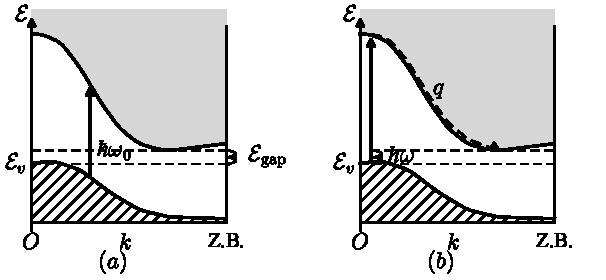
\includegraphics[width=0.72\textwidth]{fig_144.pdf}
\caption*{图 144\quad (a) 直接跃迁未必给出能隙；(b) 声子辅助跃迁。}
\end{figure}

不过，如果允许同时发射或吸收一个声子，便有可能观察到 $\hbar\omega\approx\mathcal{E}_{\mathrm{gap}}$ 的光学跃迁。这类\emph{间接}跃迁或\emph{声子辅助}跃迁（phonon-assisted transitions）很容易用二阶微扰论导出。过程分两步；例如，先通过吸收一个光子竖直地向上跃迁，然后通过发射或吸收一个波矢 $\mathbf{q}$ 足够大的声子，到达导带中相应的极小点。我们无须操心中间虚态中的能量守恒；总的条件将是

\begin{equation*}
\hbar\omega = \mathcal{E}_{\mathrm{gap}} \pm \hbar\nu_{\mathbf{q}},
\tag{8.75}
\end{equation*}

其中 $\nu_{\mathbf{q}}$ 是声子的频率。由于在能隙的尺度上 $\hbar\nu_{\mathbf{q}}$ 是个小能量（例如 0.03 eV），我们会发现吸收带似乎从 $\mathcal{E}_{\mathrm{gap}}$ 附近开始。但间接跃迁的概率比直接跃迁小得多，并且如式 (8.70) 所示，通过声子态的占据数而依赖于温度。

以上关于完整晶体中电子跃迁的讨论采用的是简单的单电子模型。然而在现实中，如图 144 那样的跃迁，其末态在导带中有一个电子之外，价带中还有一个空穴。如果这两个粒子没有立即彼此分飞开来，它们可以像 §6.7 中那样相互吸引而形成束缚态——Wannier 激子（exciton）能级——其总能量低于产生它们的那条带隙。换言之，光谱在基本吸收边之下显示出激子谱线。这一现象在离子晶体中特别显著（译注：原文作“in ionic and crystals”，疑有脱字）：其中的 Frenkel 激子虽然“小”且实际上不能移动，却具有很大的振子强度，对应于它们所源自的原子或分子激发态。
在这些材料中，电磁场与激子振幅之间的耦合可以强到足以产生极化激元（polariton）传播模式（参见 §8.3）。

杂质与不完整性的效应也使半导体和离子晶体的光学性质大大复杂化，同时也大大丰富起来。例如，人们可以观察到与带电杂质的类氢能级之间的跃迁相联系的各种吸收线（§6.4）。

色心（colour centre）中光学跃迁的理论因不完整性周围的晶格畸变而变得稍微复杂一些。由于这种畸变受到与光学活性电子的静电相互作用的影响，它必然依赖于系统的电子态。因此，不完整性的本征态必须同时用电子坐标和原子坐标来描写。但是，光学跃迁在被吸收或发射的频率的周期时间内发生，而晶格畸变到新电子态所要求的位形所需的时间却是一个动力学模的周期，比前者长得多。因此，从晶格的观点看，跃迁必须当作\emph{非绝热}的或\emph{突然}的来处理（参见 §6.11）。

这就是 Franck–Condon 原理的基础，如图 145 所示。设不完整性周围晶格的畸变可以用单一坐标 $u$ 来度量，例如离子向内或向外的“呼吸”式位移的振幅。当电子处于某态 $|a\rangle$ 时，晶格的势能在某个值 $u_a$ 处取极小，这与另一电子态 $|b\rangle$ 的平衡位移 $u_b$ 不同。从 $|a\rangle$ 到 $|b\rangle$ 的光吸收将在晶格畸变不变的情况下进行——即沿直线 $u=u_a$ “竖直地”进行。反之，发射则必须沿 $u_b$ 进行，它对应于初始电子态 $|b\rangle$ 中的平衡位移。显然，$\hbar\omega_{ab}\neq\hbar\omega_{ba}$。不过在实际上，我们还必须考虑每个势能极小点附近晶格模的热激发。声子发射会使谱线展宽，并且在高温下最终会把两个过程之间的差别抹平。

\begin{figure}[H]
\centering
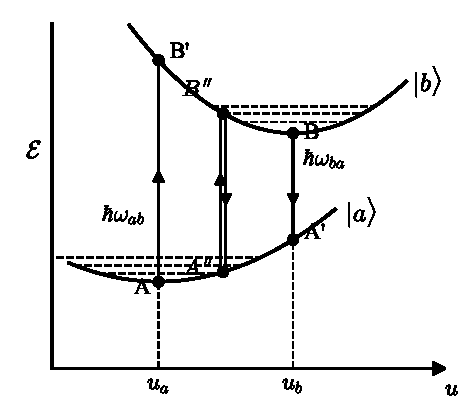
\includegraphics[width=0.72\textwidth]{fig_145.pdf}
\caption*{图 145\quad F 心处的光学跃迁，显示晶格畸变的效应：吸收 AB' 所需的能量高于发射 BA'。高温下，声子能级与两个方向的电子跃迁相结合（A'B'）。}
\end{figure}

带间光学跃迁当然在金属中也可以观察到——只是需要修正，以顾及电子未必完全填满一个带、或者可能分布于几个不同的布里渊区这一事实。这类跃迁的理论原则上遵循本节的论证——但该现象当然可能在一定程度上被电子系统的电导率所伴随的高反射率所掩盖（见 §8.6）。

另一种本质上等价于带间跃迁的现象是软 X 射线的发射。当固体中一个原子的最深能级之一上的电子被移走时，电子从其他各个能级向下跃迁，便发射出 X 射线。我们关心的是从金属价带出发的跃迁——直观上很显然，发射辐射的谱将显示出一个频带，反映出传导电子或价电子所占据的态带。

\begin{figure}[H]
\centering
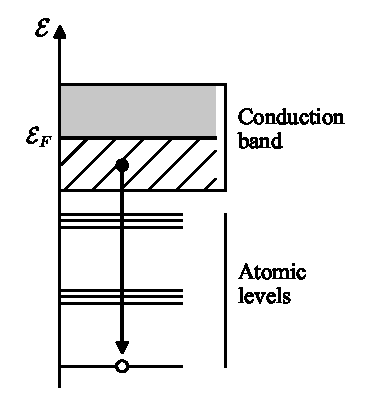
\includegraphics[width=0.72\textwidth]{fig_146.pdf}
\caption*{图 146\quad X 射线发射。}
\end{figure}

这个谱的实际形状将取决于带中态密度与相应跃迁矩阵元平方二者的乘积。众所周知，电子与电磁场之间的相互作用是通过电子的动量算符进行的（即通过电子运动产生的电流），因此必须研究如下形式的矩阵元

\begin{equation*}
\int \psi_{\mathbf{k}}^{*}(\mathbf{r})\, e^{i\mathbf{K}\cdot\mathbf{r}}\, \mathrm{grad}\,\phi_a(\mathbf{r})\,\mathrm{d}\mathbf{r},
\tag{8.76}
\end{equation*}

其中 $\phi_a$ 是失去电子的那个原子轨道，$\mathbf{K}$ 是 X 射线的波矢。与这类跃迁相联系的波长在原子距离的尺度上仍然是长的，所以这个波动因子可以忽略——而且，由于 $\phi_a(\mathbf{r})$ 是局域化的函数，不存在动量选择定则。

然而，这个矩阵元在整个带内可能有相当大的变化，视能级 $\phi_a$ 是 s 态还是 p 态而定，也视 $\psi_{\mathbf{k}}(\mathbf{r})$ 在原子内部更偏 s 型还是 p 型而定。还有来自电子间相互作用的效应。因此，发射谱的确切形状未必是态密度的直接量度，尽管它应当反映该函数的某些特征，特别是 费米能级处的锐利截止。

晶体对光或 X 射线的吸收伴随着电子被激发到更高的能级。在半导体或绝缘体中，这些激发电子通常是可以移动的，因而产生光电导（photoconductivity）。但是这样产生的载流子很容易被杂质和不完整性俘获（trapping），大量复杂的实验现象即为明证。

如果能量足够，电子可以穿越晶体表面被光电发射出去。关于光电效应的初等 Einstein 公式只告诉我们，它在表面之外具有的能量不能超过

\begin{equation*}
\mathcal{E}_{\max} = \hbar\omega - \phi_W
\tag{8.77}
\end{equation*}

因为它必须已经越过了功函数势垒 $\phi_W$（§6.9）。但能量较低的光电子必定来自晶体内 费米能量以下的能级。直接测量 $n(\mathcal{E},\omega)$——给定光子频率下发射电子的能量分布——应当能给出大量关于从占据带态到空带态的跃迁概率的信息，这类跃迁正是光吸收的成因。

为了解释这些观察结果，我们自然会构造一幅能级图（图 147），并按照图 143 的方式清点竖直的或直接的跃迁。原则上，若能同时控制 $\mathcal{E}$ 和 $\omega$，我们由此应当能获得比诸如式 (8.73) 的带间谱密度所给出的稍多一点关于能带结构的信息。实际上，许多晶体固体的光电发射谱并不符合这一模式，而似乎表现得如同

\begin{equation*}
n(\mathcal{E},\omega) \sim \rho_f(\mathcal{E})\,\rho_i(\mathcal{E}-\hbar\omega),
\tag{8.78}
\end{equation*}

仿佛在能量密度为 $\rho_i(\mathcal{E}-\hbar\omega)$ 的初态与能量为 $\rho_f(\mathcal{E})$ 的末态之间，“非直接”跃迁可以不加甄别地发生。实验在技术上很困难，但结论是明确的：尚不清楚这一与简单理论的分歧，究竟仅仅是像 L.E.E.D.（§6.9）中那样，由于发射表面附近晶体动量选择定则的失效所致，还是应归因于多电子效应。

\begin{figure}[H]
\centering
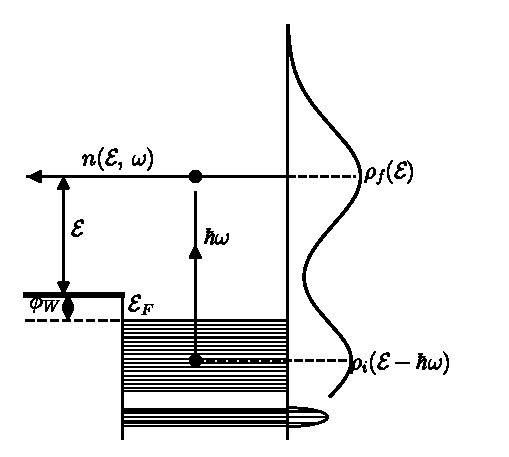
\includegraphics[width=0.72\textwidth]{fig_147.pdf}
\caption*{图 147\quad 光电发射。}
\end{figure}

\section{与传导电子的相互作用}

当固体是相对良好的导体时，光学性质会怎样？例如，假定我们在复折射率的公式 (8.7) 中忽略 $\epsilon$——这是一个对金属有效的假定。

于是我们有

\begin{equation*}
\mathsf{N}^2 = \frac{4\pi\sigma}{\omega}\, i,
\tag{8.79}
\end{equation*}

并且实部和虚部大小相等：

\begin{equation*}
\mathsf{n} + i\mathsf{k} = \left(\frac{2\pi\sigma}{\omega}\right)^{\frac{1}{2}}(1+i).
\tag{8.80}
\end{equation*}

其最显而易见的后果是，固体的反射本领变得非常高。由式 (8.19)，

\begin{equation*}
\mathsf{R} \approx 1 - 2\left(\frac{\omega}{2\pi\sigma}\right)^{\frac{1}{2}},
\tag{8.81}
\end{equation*}

这就是所谓的 Hagen--Rubens 关系。对完全反射性的偏离正比于

\begin{equation*}
\left(\frac{\omega}{2\pi\sigma}\right)^{\frac{1}{2}} \sim \left(\frac{2\omega}{\omega_p^2\tau}\right)^{\frac{1}{2}},
\tag{8.82}
\end{equation*}

其中 $\tau$ 是电导率的经典公式 (7.33) 中的弛豫时间，而 $\omega_p$ 则是电子气无处不在的等离体频率。我们知道，即使 $\omega$ 接近红外频率，这个比值也仍然相当小。

但这个初等的宏观理论假定 $\sigma$ 与频率无关。当场振荡得如此之快，以致电子来不及发生碰撞时——即当

\begin{equation*}
\omega\tau > 1.
\tag{8.83}
\end{equation*}

时——情况就不再如此。要研究这个区域，我们必须回到输运方程 (7.14)。

为了完整起见，也为了便于后面引用，让我们写下分布可以在空间和时间上变化的 Boltzmann 方程：

\begin{equation*}
e\mathbf{E}\cdot\mathbf{v}_{\mathbf{k}}\left(-\frac{\partial f^0}{\partial\mathcal{E}}\right) = \frac{g_{\mathbf{k}}}{\tau} + \mathbf{v}_{\mathbf{k}}\cdot\frac{\partial g_{\mathbf{k}}}{\partial\mathbf{r}} + \frac{\partial g_{\mathbf{k}}}{\partial t}.
\tag{8.84}
\end{equation*}

我们像 (7.17) 中那样假定一个弛豫时间。“失衡”分布 $g_{\mathbf{k}}$ 随时间的变化可以被显式地包括进来；正如从 (7.7) 所看到的，当 $\partial f_{\mathbf{k}}/\partial t$ 的所有其他贡献都被计入之后，剩下来的正是这一项。

现在设

\begin{equation*}
\mathbf{E} = \mathbf{E}_0\exp\{i(\mathbf{K}\cdot\mathbf{r}-\omega t)\},
\tag{8.85}
\end{equation*}

如 (8.3) 中那样，并设 $g_{\mathbf{k}}$ 出于“感应”（sympathy）也以同样的方式随空间和时间变化。于是，令

\begin{equation*}
g_{\mathbf{k}} = \left(-\frac{\partial f^0}{\partial\mathcal{E}}\right)\Phi(\mathbf{k})\exp\{i(\mathbf{K}\cdot\mathbf{r}-\omega t)\}.
\tag{8.86}
\end{equation*}

代入 (8.84)，得到

\begin{equation*}
e\mathbf{E}_0\cdot\mathbf{v}_{\mathbf{k}} = \frac{\Phi(\mathbf{k})}{\tau} + i\mathbf{K}\cdot\mathbf{v}_{\mathbf{k}}\,\Phi(\mathbf{k}) - i\omega\Phi(\mathbf{k}),
\tag{8.87}
\end{equation*}

其解为

\begin{equation*}
\Phi(\mathbf{k}) = \frac{e\tau\,\mathbf{v}_{\mathbf{k}}\cdot\mathbf{E}_0}{1-i\omega\tau+i\tau\mathbf{K}\cdot\mathbf{v}_{\mathbf{k}}}.
\tag{8.88}
\end{equation*}

我们的 Boltzmann 方程的线性性质使得这个初等的解成为可能。

对于电导率，如 (7.20)--(7.24) 中那样，我们有

\begin{align*}
\boldsymbol{\sigma}\cdot\mathbf{E}_0 &= \frac{e}{4\pi^3}\int \Phi(\mathbf{k})\,\mathbf{v}_{\mathbf{k}}\,\frac{dS_F}{\hbar v_{\mathbf{k}}} \\
&= \frac{e^2}{4\pi^3}\int \frac{\tau\,\mathbf{v}_{\mathbf{k}}\mathbf{v}_{\mathbf{k}}}{1-i\tau(\omega-\mathbf{K}\cdot\mathbf{v}_{\mathbf{k}})}\,\frac{dS_F}{\hbar v_{\mathbf{k}}}\cdot\mathbf{E}_0.
\tag{8.89}
\end{align*}

于是，电导率本身就有了实部和虚部；$\boldsymbol{\sigma}$ 的实部将对 $\mathsf{N}^2$ 的虚部作出贡献，而 $\boldsymbol{\sigma}$ 的虚部则看上去像是实介电常数的一部分。

对于普通的电磁波，其相速大于电子的 费米速度，我们可以略去 $\mathbf{K}\cdot\mathbf{v}_{\mathbf{k}}$ 项，它比 $\omega$ 小得多。为形式上简单起见，假定金属具有立方对称性，我们从 (8.89) 得到

\begin{align*}
\sigma(\omega) &= \frac{e^2}{12\pi^3}\int \frac{\tau v(1+i\omega\tau)}{1+\omega^2\tau^2}\,dS_F \\
&= \sigma(0)\frac{1+i\omega\tau}{1+\omega^2\tau^2},
\tag{8.90}
\end{align*}

其中 $\sigma(0)$ 是金属的普通静态电导率。

应当把这个公式代入 (8.7) 和 (8.19)。若取 $\epsilon=1$，即忽略离子的任何内部极化率，则由 (8.7)、(8.8)、(7.33) 和 (5.53)，我们得到 $\mathsf{N}^2$ 的实部和虚部

\begin{align*}
\mathsf{n}^2-\mathsf{k}^2 &= 1-\frac{4\pi\sigma(0)\,\omega\tau}{\omega(1+\omega^2\tau^2)} \\
&= 1-\frac{\omega_p^2\tau^2}{1+\omega^2\tau^2}
\tag{8.91}
\end{align*}

以及

\begin{align*}
2\mathsf{n}\mathsf{k} &= \frac{4\pi\sigma(0)}{\omega(1+\omega^2\tau^2)} \\
&= \frac{\omega_p^2\tau}{\omega(1+\omega^2\tau^2)},
\tag{8.92}
\end{align*}

其中，电子气的等离体频率再一次扮演了最重要的角色。

这个 \emph{Drude 理论}涵盖了三个不同的频率区域。

(i) $\omega\ll 1/\tau$。这是普通的低频区。$\mathsf{N}^2$ 的虚部远大于实部，因而金属强烈反射，Hagen--Rubens 关系 (8.81) 成立。吸收系数大体上与 $\omega$ 无关，而正比于电导率。$\mathsf{N}^2$ 的实部为负，其大小远大于 1。

(ii) $1/\tau\ll\omega\ll\omega_p$。这是\emph{弛豫区}（relaxation region），在此区域中 $\omega^2\tau^2$ 在 (8.91) 与 (8.92) 的分母里占了上风。吸收系数迅速下降，与 $1/\omega^2$ 成比例——而且说来奇怪，它与电导率成\emph{反}比。$\mathsf{N}^2$ 的虚部变得小于实部——但后者仍然很大且为负，如今具有如下形式

\begin{equation*}
\mathsf{n}^2-\mathsf{k}^2 = 1-\frac{\omega_p^2}{\omega^2}
\tag{8.93}
\end{equation*}

如 (5.67) 和 (8.45) 中那样。于是，金属仍然强烈反射，此时

\begin{equation*}
\mathsf{R} \approx 1-\frac{1}{\sqrt{\pi\sigma_0\tau}} \approx 1-\frac{2}{\omega_p\tau}.
\tag{8.94}
\end{equation*}

\begin{figure}[H]
\centering
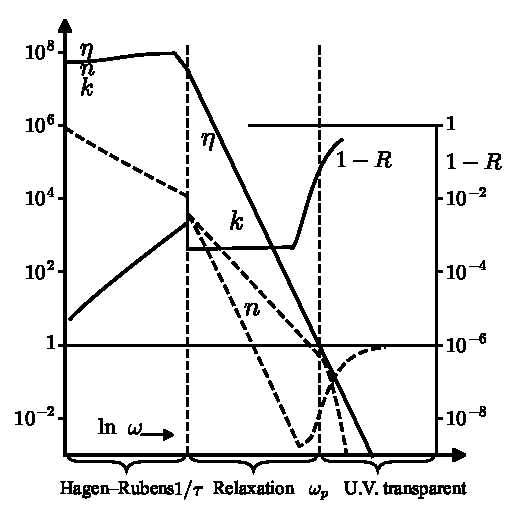
\includegraphics[width=0.72\textwidth]{fig_148.pdf}
\caption*{图 148\quad 金属光学性质的示意行为，图中示出介电常数的实部和虚部、反射系数以及吸收系数。注意频率采用对数标度。}
\end{figure}

(iii) $\omega_p\ll\omega$。$\mathsf{N}^2$ 的实部变为正数，反射本领降到零。这时金属应当显得或多或少是透明的，其吸收系数为

\begin{equation*}
\frac{2\omega\,\mathsf{n}(\omega)\,\mathsf{k}(\omega)}{c} \approx \frac{\omega_p^2}{\omega^2\tau c}.
\tag{8.95}
\end{equation*}

式 (8.91) 和 (8.92) 蕴含着 $\mathsf{n}$ 与 $\mathsf{k}$ 作为 $\omega$ 的函数之间的某些关系，而事实上这些关系并不总是得到遵守。但
这在某种程度上可以理解，只要认为积分 (8.89) 中的弛豫时间 $\tau$ 并非常数，而是在费米面上逐点变化的。这样，我们原则上可以区分出三种不同的积分
\begin{equation*}
\int \tau v\,dS_F,\quad \int \tau^2 v\,dS_F,\quad \int \frac{v}{\tau}\,dS_F, \tag{8.96}
\end{equation*}
它们对应于 $\tau(\mathbf{k})$ 在费米面上的三种不同类型的平均。没有理由认为这些不同的平均就应当全都相等。

我们还注意到，$\mathsf{N}^2$ 在高频下的实部依赖于积分
\begin{equation*}
\int v\,dS_F, \tag{8.97}
\end{equation*}
对自由电子而言，它正比于电子数目，反比于电子质量。而在态密度中出现的却是另一种类型的速度平均——调和平均
\begin{equation*}
\int \frac{dS_F}{v} \tag{8.98}
\end{equation*}
如 (4.6) 中那样。这两类平均之间的差别，可以提供关于电子速度在费米面上各向异性的信息。用一个与“光学质量”相联系的因子去“修正” (8.97) 的观测值并不明智；事后往往发现，这样得到的因子与为使 (8.98) 符合电子比热的自由电子公式所需要的“热质量”大不相同。“一切费米面都是球面”这一隐含假设，即便对一价金属也常常站不住脚。

\section{反常趋肤效应}

Hagen–Rubens 关系 (8.81) 还可能以另一种方式失效。由 (8.79) 给出的吸收系数非常高，电磁波进入金属后很快就被衰减掉了。由 (8.10) 与 (8.80) 得出的阻尼距离的数量级为
\begin{align*}
\delta &= \frac{c}{\mathsf{k}\omega} \\
&= \frac{c}{(2\pi\sigma\omega)^{\frac{1}{2}}}\,. \tag{8.99}
\end{align*}
这个现象在经典电动力学中早已众所周知，称为趋肤效应（skin effect）。我们把由 (8.99) 给出的 $\delta$ 称为经典趋肤深度（classical skin depth）$\delta_{\mathrm{cl}}$。

在高频下，$\delta$ 可以变得非常小。如果我们在低温下取一块纯度极高的金属，就会发现趋肤深度可以变得远小于电子平均自由程 $\Lambda$。电导率的普通理论这时不再有效；作用在载流子上的有效场，在载流子于两次碰撞之间所走过的距离上变化急剧。

为了处理这种情形，我们必须尝试求解 $g_{\mathbf{k}}$ 随空间变化的 Boltzmann 方程。如果忽略 $\mathbf{E}$ 与 $g_{\mathbf{k}}$ 的时间变化（这一现象很容易在远低于上述弛豫区起始处的频率下观察到），那么仿照 (8.84)，我们得到
\begin{equation*}
e\mathbf{E}(\mathbf{r})\cdot\mathbf{v}_{\mathbf{k}}\left(-\frac{\partial f^0}{\partial\mathcal{E}}\right) = \frac{g_{\mathbf{k}}}{\tau} + \mathbf{v}_{\mathbf{k}}\cdot\frac{\partial g_{\mathbf{k}}}{\partial\mathbf{r}} \tag{8.100}
\end{equation*}
作为待求解的 $g_{\mathbf{k}}$ 的微分方程。

求解 (8.100) 最直接的做法——它适用于涉及表面、薄膜、细丝等等的各类问题——是采用 Chambers 公式（Chambers formula）
\begin{equation*}
g(\mathbf{v},\mathbf{r}) = \frac{e}{v}\left(-\frac{\partial f^0}{\partial\mathcal{E}}\right)\int^{\mathbf{r}} \mathbf{v}\cdot\mathbf{E}(\mathbf{r}')\,e^{-s'/\tau v}\,ds'. \tag{8.101}
\end{equation*}
用完全形式化的办法证明这是微分方程的一个解并不十分困难；它只不过是方程 $dy/dx+\alpha y=f(x)$ 的通常求解公式的一个直接推广。

从物理上讲，它意味着在点 $\mathbf{r}$ 处、沿方向 $\mathbf{v}$ 的电子电流，取决于对该电流有贡献的那些电子此前走过的历史。积分并不是遍及整个空间，而只是沿通过 $\mathbf{r}$ 点、方向为 $\mathbf{v}$ 的轨道向回追溯到距离 $s'$ 处。这样，在 $\mathbf{r}'$ 点处电子受到力 $e\mathbf{E}(\mathbf{r}')$ 而加速。但由于弛豫过程，这份贡献随时间衰减；指数因子度量的正是这种效应沿轨道随距离的变化。这个半经典公式在原理上与 Kubo 公式 (7.15) 密切相关，在那里我们同样要对体系此前的历史作积分。

由 (8.101)，可以用通常的公式 (7.20) 计算总电流。但我们注意到，这个电流将是 $\mathbf{r}$ 的函数——同时也是函数 $g(\mathbf{v},\mathbf{r})$ 的边界条件的函数。于是，存在一个积分方程，把 $\mathbf{J}(\mathbf{r})$ 定义为电场分布 $\mathbf{E}(\mathbf{r})$ 的泛函。另一方面，这两个量又由如下比 (8.2) 更一般形式的 Maxwell 方程联系起来：
\begin{align*}
\nabla^2\mathbf{E} &= \frac{4\pi}{c^2}\frac{d\mathbf{J}}{dt} \\
&= \frac{4\pi i\omega}{c^2}\,\mathbf{J}(\mathbf{r}) \tag{8.102}
\end{align*}
（略去通常的位移电流）。这样一来，人们可以求解由 (8.101) 与 (8.102) 导出的积分微分方程，得出表面附近 $\mathbf{J}(\mathbf{r})$ 与 $\mathbf{E}(\mathbf{r})$ 的分布。

这个方程的精确解相当繁复，而且依赖于边界条件——它取决于电子在表面是被镜面反射，还是在表面受到无规散射。具体的公式并不如其物理诠释来得重要。事实是，并非所有电子都参与了电磁波的吸收和反射。只有在趋肤深度内跑完大半段平均自由程 $\Lambda$ 的那些电子，才能从
\begin{figure}[H]
\centering
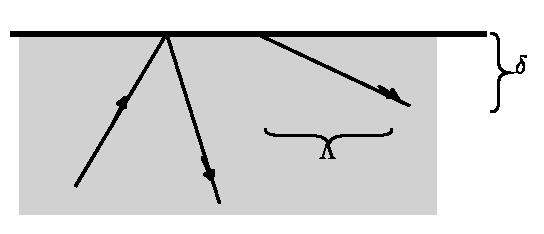
\includegraphics[width=0.72\textwidth]{fig_149.pdf}
\caption*{图 149\quad 只有处于趋肤深度内的电子才是“有效的”。}
\end{figure}
电场中汲取可观的能量。例如，若趋肤深度为 $\delta'$，则可以认为只有份额为 $\delta'/\Lambda$ 的电子对电导是\emph{有效}的。我们可以写出
\begin{equation*}
\sigma' = \frac{3}{2}\,\beta\,\frac{\delta'}{\Lambda}\,\sigma_0 \tag{8.103}
\end{equation*}
作为表观电导率——数 $\beta$ 不过是个“凑算因子”（fudge factor）。

但这样一来，按照 (8.99)，具有这一电导率的表面自身的趋肤深度就应为
\begin{align*}
\delta' &= \frac{c}{(2\pi\sigma'\omega)^{\frac{1}{2}}} \\
&= \frac{c}{\left(2\pi\,\frac{3}{2}\,\beta\,\frac{\delta'}{\Lambda}\,\sigma_0\,\omega\right)^{\frac{1}{2}}}\,, \tag{8.104}
\end{align*}
由此可解出 $\delta'$，进而解出 $\sigma'$。于是
\begin{equation*}
\sigma' = \left(\frac{9\beta^2}{8\pi}\right)^{\frac{1}{3}} \frac{1}{\omega^{\frac{1}{3}}} \left(\frac{c\sigma_0}{\Lambda}\right)^{\frac{2}{3}}; \tag{8.105}
\end{equation*}
有效电导率将表现得如同 $\omega^{-\frac{1}{3}}$，但却与电子平均自由程无关——它与普通静态电导率 $\sigma_0$ 中的相应因子相消了。这时我们就处于反常趋肤效应（anomalous skin effect）的条件下。实践上人们的做法是把金属表面做成共振腔的一部分，然后观察腔的共振性质所受到的影响。比如说，可以测量表面阻抗（surface impedance），按 §8.1 的记号，它就是
\begin{equation*}
\mathbf{Z}(\omega) = -4\pi i\omega\,\frac{E(z)}{(\partial E/\partial z)}\bigg]_{z=0} = \frac{4\pi c}{\mathsf{N}} \tag{8.106}
\end{equation*}
在反常极限下，金属表观光学性质的理论中还有其他一些变化可以推演出来，特别是当频率进入弛豫区时。例如，若表面是“粗糙”的，则电子在表面的实际散射会从反射波中额外吸收功率——这一贡献可与前一节中算出的（忽略这种散射时的）效应同样大小。

然而，反常趋肤效应最有意思的性质，是它对费米面几何形状的依赖。如上所述，只有那些几乎平行于表面运动的电子才对电导“有效”。如果样品是单晶，这些电子便来自环绕费米面的一条窄带。倘若费米面高度各向异性，那么在金属晶体的不同切面上、场的不同取向下测量，我们理应看到不同的表面阻抗值。

所要测量的几何性质，可以通过把“无效性概念”（ineffectiveness concept）(8.103) 加以推广而导出。我们假定只需考虑速度矢量与 $(x,y)$ 平面（它界定金属边界）的平行度相差 $\pm\beta\delta'/\Lambda$ 角之内的电子（取电场沿 $x$ 方向）。

在有效电子带的某个一般点 $P$ 处，速度 $\mathbf{v}$ 与 $\mathbf{E}$ 成 $\theta$ 角。带的该处宽度将为 $2\beta\delta'|\rho|/\Lambda$，其中 $|\rho|$ 是在 $\mathbf{v}$ 与 $z$ 轴所定平面内的曲率半径。带周长上长为 $ds$ 的一段元，于是对应于费米面上的一块面积
\begin{equation*}
dS = \frac{2\beta\delta'|\rho|}{\Lambda}\,ds, \tag{8.107}
\end{equation*}
并且显然会按照通常的公式 (7.23) 对 $x$ 方向的电导作出贡献：
\begin{align*}
d\sigma'_{xx} &= \frac{e^2}{4\pi^3\hbar}\,\tau v_x\,dS_x \\
&= \frac{e^2}{4\pi^3\hbar}\,\Lambda\cos\theta\,\frac{2\beta\delta'|\rho|}{\Lambda}\,\cos\theta\,ds. \tag{8.108}
\end{align*}
\begin{figure}[H]
\centering
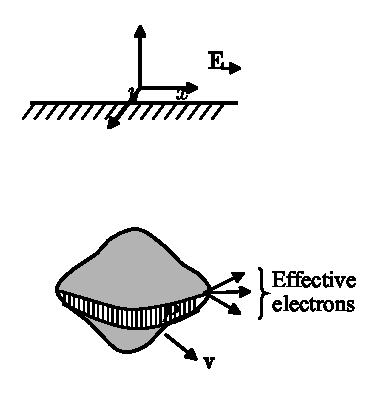
\includegraphics[width=0.72\textwidth]{fig_150.pdf}
\caption*{图 150\quad 费米面上由有效电子构成的带。}
\end{figure}
于是，金属的总表观电导率将为
\begin{align*}
\sigma' &= \frac{e^2\beta\delta'}{2\pi^3\hbar}\int |\rho|\cos^2\theta\,ds \\
&= \frac{e^2\beta\delta'}{2\pi^3\hbar}\oint |\rho_y|\,dk_y, \tag{8.109}
\end{align*}
其中 $\rho_y$ 表示费米面沿带的、平行于 $(x,z)$ 平面的截面的曲率半径，积分遍及带周围动量分量 $k_y$ 的取值范围。这就是我们代进 (8.104) 里的量，随后分别解出 $\delta'$ 与 $\sigma'$。更完整的分析表明
\begin{equation*}
\beta = \frac{8\pi}{3\sqrt{3}} \tag{8.110}
\end{equation*}
正是这个任意的“凑算因子”的合适数值。
这个结果的美妙之处在于，表面阻抗既不依赖于电子的平均自由程，也不依赖于电子的速度，而只依赖于绕一条明确定义的带积分出来的局部曲率。积分 (8.109) 对曲率半径大的区域特别敏感——也就是说，对费米面上相对平坦的部位特别敏感。因此，它提供的信息在一定程度上与其他种种“效应”互补，那些效应往往依赖于细枝末节以及费米面上互不相连的小块碎段。然而，要把一个给定费米面与一组沿不同取向的带算出的 (8.109) 型积分值之间的关系反演出来并非易事；通常不得不经过一番繁琐的试错手续。

\section{超声衰减}

高频弹性波因与金属中传导电子相互作用而衰减，其理论虽然算不上严格的“光学”性质，却最自然地放到本章来讨论。固体中的声波会产生电场，并以与电磁波大体相同的方式加速电子。但声速比光速小得多——甚至比电子的费米速度还要小——因而可以观察到某些特殊的效应。

在普通的低频区，衰减可以借助初等动理学理论（kinetic theory）来计算。一个由电子组成的气体，设其质量为 $m$、数密度为 $n$、平均速度为 $v_F$、平均自由程为 $\Lambda$，将具有黏度（viscosity）
\begin{equation*}
\eta = {\textstyle\frac{1}{3}}\,nm\Lambda v_F. \tag{8.111}
\end{equation*}
这个黏度可以作为一项纳入作用在介质体元上的力的普通经典方程。频率为 $\omega$ 的纵向弹性波的衰减常数便求出为
\begin{equation*}
\alpha = \frac{4}{5}\,\frac{\omega^2}{Ds^3}\,\eta, \tag{8.112}
\end{equation*}
其中 $D$ 是质量密度，$s$ 是声速。这些结果可以合并成各种不同的形式，例如按电导率 (7.33) 写成
\begin{equation*}
\alpha = \frac{4}{15}\,\frac{\omega^2 m v_F^2}{e^2 D s^3}\,\sigma, \tag{8.113}
\end{equation*}
如果金属非常纯，而在低温下进行测量，电子的弛豫时间会大为增长。然而，用超声波仍然难以进入 $\omega\tau>1$ 的弛豫区。
不过，正因为声速远小于费米速度，我们有可能使平均自由程长于声波的波长，即做到
\begin{equation*}
q\Lambda > 1. \tag{8.114}
\end{equation*}
为了讨论这种情形，我们回到 (8.89)，在那里我们针对在空间和时间上都作正弦变化的电场，构造了 Boltzmann 方程解的一个公式。实际上，我们求得了一个广义电导率
\begin{equation*}
\boldsymbol{\sigma}(\mathbf{q},\omega) = \frac{e^2}{4\pi^3}\int \frac{\tau\mathbf{v}\mathbf{v}}{1-i\tau(\omega-\mathbf{q}\cdot\mathbf{v})}\,\frac{dS_F}{\hbar v}. \tag{8.115}
\end{equation*}
在 §8.6 中讨论这个公式时，我们取了 $q=0$，理由是电磁波的速度如此之大，以致其波数可以取作近乎为零。但是，当电场是由
\begin{figure}[H]
\centering
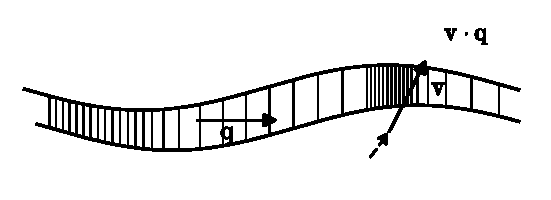
\includegraphics[width=0.72\textwidth]{fig_151.pdf}
\caption*{图 151\quad 冲浪共振。}
\end{figure}
声波产生时——声波比电子传播慢得多——这一项就必须保留。这时，电导率的实部主要来自费米面上 $\omega\sim\mathbf{q}\cdot\mathbf{v}$ 的区域。这等于换一种说法：电子速度在波传播方向上的分量等于声速。

这就是所谓的冲浪共振（surf-riding resonance）。恰好位于波峰上的电子，可以沿几乎垂直于波传播矢量的方向行进，从而继续从场中汲取能量。显然，费米面上只有少数电子能满足这一条件。如果我们把 $\omega$ 完全略去，它便在费米面上定出一条电子速度垂直于 $\mathbf{q}$ 的带——这条带与反常趋肤效应理论（§8.7）中定义的那条带形状完全相同。

在 $q\Lambda\gg1$ 的极限下计算 (8.115) 并不困难。带的有效宽度取决于当我们离开准确共振位置时 $\tau\mathbf{q}\cdot\mathbf{v}$ 增长的速率。$\tau$ 的值越大，带就变得越窄。正如 (8.107) 中那样，“有效”面积元正比于表面的局部曲率半径，反比于 $\Lambda$。
例如，用初等微分几何可以证明，在 $q\Lambda\gg1$ 的极限下有精确公式
\begin{equation*}
\sigma_{xx}(\mathbf{q},0) = \frac{e^2}{4\pi^3\hbar q}\oint |\rho_y|\,dk_y, \tag{8.116}
\end{equation*}
其中方向 $x$ 与 $y$ 都垂直于传播方向 $\mathbf{q}$，其余符号与 (8.109) 中完全相同。

这个公式的有趣之处在于它不依赖于 $\Lambda$。必须存在某种使电子最终受到散射的机制，这一点至关重要；但在这一极限下，
\begin{figure}[H]
\centering
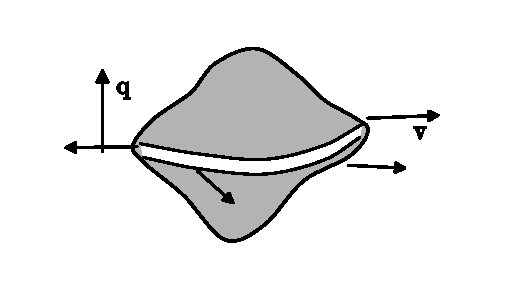
\includegraphics[width=0.72\textwidth]{fig_152.pdf}
\caption*{图 152\quad 与声子 $\mathbf{q}$ 相互作用的电子带。}
\end{figure}
散射的强弱却无关紧要。这正是我们在 §8.7 中已经遇到过的情形。事实上，人们可以用 (8.116) 作为出发点，完整地推导出反常趋肤效应的公式 (8.109)，连凑算因子 $\beta$ 的取值也包括在内。这实质上是把由 Maxwell 方程导出的关系 (8.102) 用 Fourier 分量表示出来，并且计入顾及电子在金属表面处行为的边界条件。

如果我们能单用 (8.116) 就建立起超声衰减的理论，那将是十分惬意的。测量沿各个方向穿过单晶传播的波的衰减，这一实验在技术上显然要比沿各种取向切出晶体表面、并在测量表面阻抗的同时保持它们清洁完好容易得多。

遗憾的是，这并不能给出关于费米面形状的直接信息。衰减确实会趋向一个与电子平均自由程无关的值——(8.113) 不再成立——但其数值大小取决于电子与格波耦合的细节。换句话说，电子因晶格位移或晶格应变而感受到的电场无法直接计算，而且在费米面上各处不同。
可以设想，需要在 (8.116) 的被积函数中插入一个形变势（deformation potential）——即 §6.14 中讨论过的那一类——但它要复杂得多；比如说，在多连通的费米面上，它远不像在简单的自由电子金属中那样容易用寥寥几个参数表达出来。

自由载流子引起的超声衰减也可以在半导体中出现。没有对称中心的离子型材料——例如 III–V 或 II–VI 族化合物（§4.2）——通常是压电性的（piezo-electric）。局部应变 $W_{ij}(\mathbf{r})$ 会产生一个局部电场
\begin{equation*}
\delta E_k(\mathbf{r}) = \sum_{ij}\beta_{ijk}\,W_{ij}(\mathbf{r}) \tag{8.117}
\end{equation*}
它是 (6.95) 的形变势之外的一项。这个由宏观声波携带的电场行波作用于载流子，在达到相当高的微波频率之前，它是主要的相互作用机制。此时现象的细节将取决于压电张量 $\beta_{ijk}$ 在声波偏振矢量上的投影分量。

在电导率相对较低的介质中，超声声子束把动量传递给载流子，由此产生的声电场（acousto-electric field）可以直接观测到。这显然是声子曳引效应（§7.11）的逆过程。一个密切相关的现象，是沿超声束施加直流电场而使声得到声电放大（acousto-electric amplification）。这可以看作微波激射（maser）作用的一种形式：来自电场的能量使载流子分布失去平衡，随后这一分布受激发而相干地发射声子。我们还可以注意到它与 Cerenkov 辐射的类似之处：电场使载流子获得一个超过声速的漂移速度 (7.31)，从而允许在能量与动量同时守恒的条件下直接产生声子。

上面的推导都建立在对 Boltzmann 方程的准经典处理之上。但同样的结果也可以从量子理论得到——有人也许会说，那样更严格。例如，考虑在从态 $\mathbf{k}$ 到态 $\mathbf{k}+\mathbf{q}$ 的跃迁中吸收一个频率为 $\omega$ 的声子的能量条件 (2.101)。它给我们
\begin{align*}
\hbar\omega &= \mathcal{E}(\mathbf{k}+\mathbf{q}) - \mathcal{E}(\mathbf{k}) \\
&\approx \mathbf{q}\cdot\frac{\partial\mathcal{E}(\mathbf{k})}{\partial\mathbf{k}} \\
&= \hbar\mathbf{q}\cdot\mathbf{v}_{\mathbf{k}}, \tag{8.118}
\end{align*}
它与 (8.115) 本质上相同。换句话说，“冲浪共振”无非是电子–声子相互作用的一个初级过程，正如 §§2.8、6.13 中所讨论的那样。

另外，(8.115) 还可以从一个完全不同的出发点导出。让我们把分母写成
\begin{equation*}
1-i\tau(\omega-\mathbf{q}\cdot\mathbf{v}) = \frac{i\tau}{\hbar}\bigl\{\mathcal{E}(\mathbf{k}+\mathbf{q}) - \mathcal{E}(\mathbf{k}) - \hbar\omega - i\hbar\alpha\bigr\}, \tag{8.119}
\end{equation*}
其中 $\alpha=-1/\tau$。我们认出，这正是 (5.16) 中以及第 5 章其他地方出现的那种求和的分母。稍加变换，并利用 (8.118)，我们发现可以写成
\begin{equation*}
\epsilon(\mathbf{q},\omega) \approx 1 + \frac{4\pi i\sigma_l(\mathbf{q},\omega)}{\omega} \tag{8.120}
\end{equation*}
当 $q$ 和 $\omega$ 都很小时。这里 $\sigma_l$ 指纵向电导率——即 $\boldsymbol{\sigma}$ 在声子传播方向上的分量。

换言之，我们重新导出了 (8.7)。正如在 §5.1 中计算的那样，电子气的复介电常数已经把电导率作为其虚部包含在内。在 (5.1) 中我们把 $-\alpha$ 取作微扰场的一个任意衰减常数——而把它认同为 $1/\tau$ 显然是恰当的。(5.16) 之中竟然凝聚了多得惊人的物理内容。

 % 本文件由 scripts/assemble.py 自动装配，勿手改（改 parts/ 后重跑）
% 第9章 费米面

\chapter{费米面}

\epigraphbook{你以这样一副可疑的形貌前来。}{Hamlet}

\section{强磁场}

一般说来，高温下金属的电子性质是对整个费米面上的速度、波函数、跃迁概率等量所作的复杂平均。除了由 Kohn 效应（§5.4）和正电子湮没（§5.8）得到的一些模糊而零碎的信息之外，要根据实验观测真正描绘出这个面，就得使用纯净的样品，并在低温下工作，使电子的散射不至于把现象弄模糊。当电子的弛豫时间非常短时，费米面是否还能恰当地说成“存在”，甚至都是可疑的。例如，平均自由程为 $\Lambda$ 的电子，其动量的不确定度约为 $\hbar/\Lambda$ 的量级；在高温下，这个不确定度很可能大到足以同倒格子空间中能量面的某些细致结构相比拟。

我们已经讨论过反常趋肤效应（§8.7）。关于费米面的几乎所有其他研究都有赖于强磁场的使用。磁场对一个电子态的作用由式 (6.40) 给出：
\begin{equation*}
\dot{\mathbf{k}}=\frac{e}{c\hbar}\,\mathbf{v}\wedge\mathbf{H}. \tag{9.1}
\end{equation*}
这意味着矢量 $\mathbf{k}$ 的变化是
\begin{itemize}
\item[(i)] 垂直于 $\mathbf{H}$ 的方向；
\item[(ii)] 垂直于 $\mathbf{v}$，而 $\mathbf{v}$ 本身又垂直于能量面。
\end{itemize}
因此，$\mathbf{k}$ 必然被限制在\emph{轨道}（orbit）上，即由费米面同垂直于 $\mathbf{H}$ 的平面相交所得的曲线。磁场只是驱使代表点沿这条轨道环行，而不改变能量。

如果电子不被散射，它环行一周所经历的时间为
\begin{equation*}
\frac{2\pi}{\omega_H}=\frac{c\hbar}{eH}\oint\frac{dk}{v_{\perp}}, \tag{9.2}
\end{equation*}
其中 $v_{\perp}$ 是 $\mathbf{v}$ 在垂直于 $\mathbf{H}$ 的平面内的分量，取在 $\mathbf{k}$ 点处。
相应的频率 $\omega_H$ 称为回旋频率（cyclotron frequency）。对于自由电子，由初等几何可得
\begin{equation*}
\oint\frac{dk}{v_{\perp}}=\frac{m}{\hbar}\oint\frac{dk}{k_{\perp}}=\frac{2\pi m}{\hbar}, \tag{9.3}
\end{equation*}
于是
\begin{equation*}
\omega_H=\frac{eH}{mc}. \tag{9.4}
\end{equation*}
\begin{figure}[H]
\centering
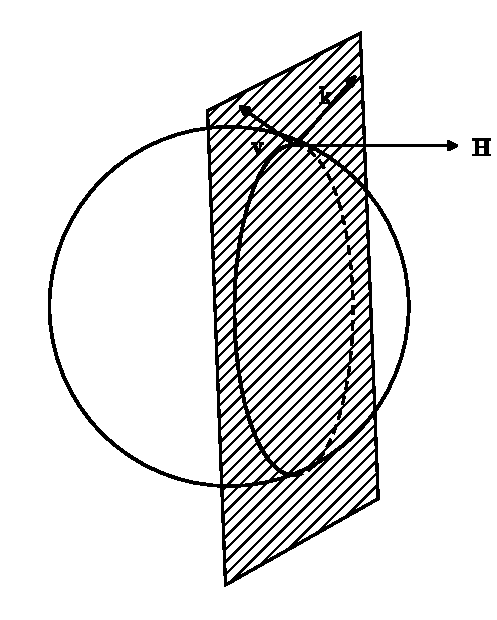
\includegraphics[width=0.72\textwidth]{fig_153.pdf}
\caption*{图 153\quad 磁场中电子的“轨道”。}
\end{figure}
\begin{figure}[H]
\centering
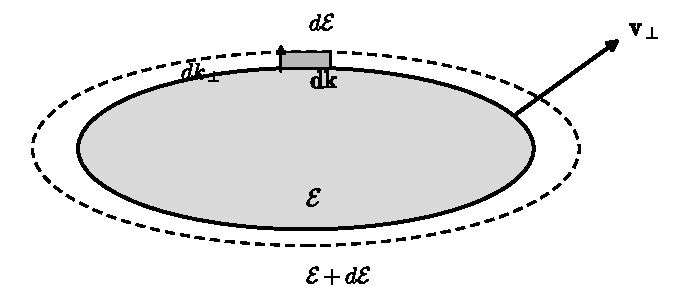
\includegraphics[width=0.72\textwidth]{fig_154.pdf}
\caption*{图 154\quad （原书此图无图注。）}
\end{figure}

习惯上还要再定义另一种“有效质量”——回旋质量（cyclotron mass）$m_H^{*}$，使得
\begin{equation*}
\omega_H=\frac{eH}{m_H^{*}c}. \tag{9.5}
\end{equation*}
应当注意，这个质量并不就是电子的动力学质量。它是轨道的属性，而不是某个特定电子态的属性。

回旋质量有一个有用的几何定义，它来自式 (6.2) 中隐含的一个事实：
\begin{equation*}
v_{\perp}=\frac{1}{\hbar}\frac{d\mathcal{E}}{dk_{\perp}}, \tag{9.6}
\end{equation*}
其中 $dk_{\perp}$ 是 $k$ 在轨道平面内、沿垂直于费米面方向的增量。由式 (9.2) 和式 (9.5) 可得（图 154）
\begin{align*}
m_H^{*}&=\frac{eH}{c}\,\frac{1}{2\pi}\,\frac{c\hbar}{eH}\oint\frac{dk}{v_{\perp}}\\
&=\frac{\hbar^{2}}{2\pi}\oint\frac{dk_{\perp}}{d\mathcal{E}}\,dk\\
&=\frac{\hbar^{2}}{2\pi}\frac{\partial\mathcal{A}}{\partial\mathcal{E}}, \tag{9.7}
\end{align*}
其中 $\mathcal{A}$ 是轨道在垂直于 $\mathbf{H}$ 的平面内所围的面积。

\section{回旋共振}

自然会想到：电子的这种周期运动可以通过与频率合适的电磁场发生共振而被探测到。唯一的条件是，电子在被散射之前至少要沿轨道环行一周。要为系统对沿磁场轴向传播的圆偏振电磁波的响应建立一个形式理论，是相当容易的。

例如，我们用一组新变量来标记 k 空间。一个点 $\mathbf{k}$ 按如下方式确定：
\begin{itemize}
\item[(i)] 能量 $\mathcal{E}(\mathbf{k})$；在磁场中它保持不变。
\item[(ii)] $\mathbf{k}$ 沿磁场方向的分量 $k_H$；它也保持不变。
\item[(iii)] 一个“相变量” $\phi$，由沿轨道的、与式 (9.2) 中出现的同一种积分来定义，即
\end{itemize}
\begin{equation*}
\phi=\omega_H\frac{c\hbar}{eH}\int^{\mathbf{k}}\frac{dk}{v_{\perp}}. \tag{9.8}
\end{equation*}
这是一个便利的变量，因为在磁场作用下它自动以恒定速率增大：
\begin{equation*}
\dot{\phi}=\omega_H, \tag{9.9}
\end{equation*}
且当环行一整圈时 $\phi=2\pi$。

我们可以把这些变量用作 Boltzmann 方程的坐标框架。可以把式 (7.10) 中的“失衡”部分 $g_{\mathbf{k}}$ 表示为 $(\mathcal{E},k_H,\phi)$ 的函数。如果像式 (8.84) 中那样假定一个弛豫时间，那么只需再添一项
\begin{equation*}
\left.\frac{\partial f}{\partial t}\right]_{\text{mag.}}=\dot{\phi}\,\frac{\partial g}{\partial\phi}=\omega_H\frac{\partial g}{\partial\phi} \tag{9.10}
\end{equation*}
就能把磁场对电子分布的影响包括进来。这与式 (7.137) 中所用的表达式等价，只是更为紧凑，在那里磁场被假定是小的。

我们取一个频率为 $\omega$ 的随时间变化的场，并忽略 $\mathbf{E}$ 随空间的变化。再仿照式 (8.86)，假定
\begin{equation*}
g(\mathcal{E},k_H,\phi)=\left(-\frac{\partial f^0}{\partial\mathcal{E}}\right)\Phi(k_H)\,e^{i(\phi-\omega t)}, \tag{9.11}
\end{equation*}
即电子分布（即便不是每一个单个电子）实际上以外场的频率被驱动沿轨道环行。于是我们的 Boltzmann 方程
\begin{equation*}
e\mathbf{E}\cdot\mathbf{v}\left(-\frac{\partial f^0}{\partial\mathcal{E}}\right)=\frac{g}{\tau}+\omega_H\frac{\partial g}{\partial\phi}+\frac{\partial g}{\partial t} \tag{9.12}
\end{equation*}
具有解
\begin{equation*}
\Phi(k_H)=\frac{e\tau\,\mathbf{v}\cdot\mathbf{E}}{1+i(\omega_H-\omega)\tau}, \tag{9.13}
\end{equation*}
和先前一样，偏离正比于场的强度，但除非外加频率与系统的固有回旋频率相同，它将带着相位差沿轨道跟随转动。

正如式 (8.90) 那样，金属的行为就好像它具有如下电导率：
\begin{equation*}
\sigma(\omega)=\sigma(0)\,\frac{1-i(\omega_H-\omega)\tau}{1+(\omega_H-\omega)^{2}\tau^{2}}. \tag{9.14}
\end{equation*}
观测材料的表面电阻、反射本领、吸收等，就会在频率 $\omega=\omega_H$ 处看到一条宽度为 $1/\tau$ 的回旋共振线。这一结果与式 (8.51) 中的光学共振理论之间的类似是显然的。对自由电子，通过对运动方程的简单分析不难得到这个结果——但我们在这里证明的结果要略微更普遍一些，尽管对于任意费米面它并不完全精确，因为在那里的假设 (9.11) 忽略了变量 $\phi$ 的高次谐波。

这一公式是对旋转方向与磁场中电子固有回旋运动\emph{相同}的圆偏振波束而言的。
显而易见，从几何上的考虑即可知道：偏振方向相反的波束，其公式将以 $+\omega$ 代替 $-\omega$；这样就不会发生共振。但考虑 $\sigma(\omega)$ 的\emph{虚部}，它对复折射率 (8.7) 的\emph{实部}有贡献，从而改变电磁波的相速。对于沿磁场方向传播的线偏振波束，两个圆偏振分量以不同的速度行进，因此当波穿过晶体时，偏振面便不断旋转。这就是众所周知的 Faraday 效应。

对半导体而言，这几乎就是描述回旋共振所需的全部理论。载流子无论电子还是空穴，都占据着 $\mathcal{E}(\mathbf{k})$ 函数的一些小口袋，它们位于能带的极小或极大处。在这些邻域内，能量面通常是椭球面（参见 §2.5）；可以证明，$\omega_H$ 在椭球的所有平行截面上都是相同的，因此能观测到式 (9.14) 所预言的谱线。当然，$\omega_H$ 随取向而变化，由此可以提供关于椭球各轴的信息。在区中心价带极大附近情形更为复杂，那里能级被自旋–轨道相互作用（§3.9）所分裂，但分析基本上仍循上述路线进行。

对金属来说，有两个似乎横亘在前的困难。为了分辨共振线，我们需要在高频下工作，使 $\omega\tau\gg 1$。在这些条件下，趋肤深度非常小——实际上我们已处在 §8.7 的反常区域。于是，磁场中电子的螺旋轨迹在真实空间中的半径，将远大于电场所能穿透的距离。

这提示我们应当把磁场垂直于金属表面施加，这样发生共振的电子就是趋肤层内的“有效”电子，能够吸收功率。但对这种情形作一分析就会发现，“共振”被抹平到几乎无法探测。把式 (9.14) 代入式 (8.7)，原则上可以看出这是如何发生的。正如式 (8.91) 那样，复折射率有很大的虚部，主要原因在于 $N^{2}$ 的实部很大且为负。金属的电导太高了；我们所能测量的只是其反射本领的微小亏损，如式 (8.94) 那样。要看到在半导体中很容易探测到的那种共振线，我们就必须工作在等离体频率 $\omega_p$ 之上，而这将需要极其巨大的磁场。

另一方面，假设我们手头有“好的”回旋材料，例如 4°K 的极纯 Na，在几千奥斯特的磁场中其 $\omega_H\tau\gg 1$。如果我们以非常低的频率工作——每秒不过几个周期——就可以使折射率 (8.7) 接近于实数，并观察电磁波穿过一块金属板的传播。这可由式 (9.14) 得出；令 $\omega\ll\omega_H$，我们得到
\begin{align*}
\mathsf{N}&=\left(\epsilon+\frac{4\pi i\sigma(\omega)}{\omega}\right)^{1/2}\\
&\approx\left(\frac{4\pi\sigma(0)}{\omega\omega_H\tau}\right)^{1/2}=\left(\frac{4\pi nec}{H\omega}\right)^{1/2}=\frac{\omega_p}{(\omega\omega_H)^{1/2}}. \tag{9.15}
\end{align*}
结果表明这是一个非常大的数，约为 $10^{10}$ 的量级。因此波在金属中仅以每秒几厘米的速度行进——一种以“人”的长度和时间尺度来衡量的现象。在式 (9.15) 中，重要的是 $\omega$ 与 $\omega_H$ 应当同号；式 (9.8) 和式 (9.11) 确立的约定意味着，我们所处理的是与电子回旋运动同相位旋转的圆偏振波。这样，一个螺旋波（helicon）模就把电子气的回旋激发与等离激元激发结合在一起。遗憾的是，从这种现象所能获得的信息是有限的，因为式 (9.15) 在一级近似上并不仅仅依赖于费米面的几何。在补偿半导体（§4.6）中，电子与空穴的螺旋波项彼此抵消，只剩下描述 Alfvén 波传播的高阶项——这是天体物理中另一种人们熟悉的磁–等离体现象。

事实证明，当磁场\emph{平行}于表面时可以探测到很强的共振。这就是 Azbel'–Kaner 共振，其成因如下。电子沿螺旋轨道回旋，其轴向（比如说沿 $x$ 方向）与表面平行。每回旋一周，它都进入趋肤深度一次，“看见”振荡的电场。如果它每次返回时都与场同相位，它就会从场中获得能量，从而观察到“共振”。

推导一个描述这种现象的公式并不困难。我们把普遍的动理学表达式 (8.101) 写成如下形式：
\begin{equation*}
\mathbf{J}(\mathbf{r},t)=\frac{e^{2}}{4\pi^{3}\hbar}\int\mathbf{v}\left\{\int_{-\infty}^{t}\mathbf{v}(\mathbf{r}',t')\cdot\mathbf{E}(\mathbf{r}',t')\,e^{-(t-t')/\tau}\,dt'\right\}\frac{dS_F}{v}. \tag{9.16}
\end{equation*}
这里我们已经对费米面积分，得到总电流。但我们仍然明显地保留了论证的主要特征
\begin{figure}[H]
\centering
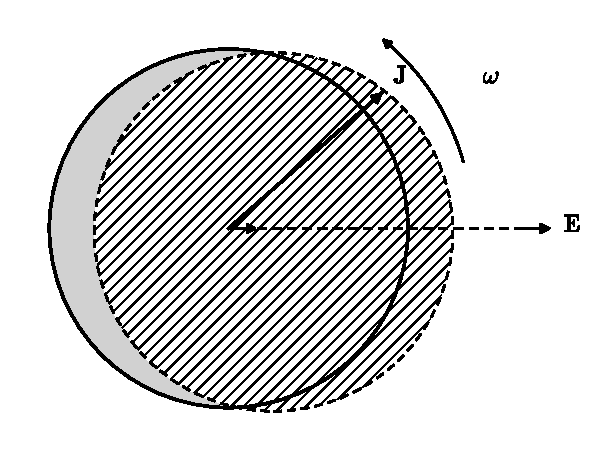
\includegraphics[width=0.72\textwidth]{fig_155.pdf}
\caption*{图 155\quad 电场使费米分布发生位移。这个位移被驱动沿费米面环行，并随时间衰减。}
\end{figure}
\begin{figure}[H]
\centering
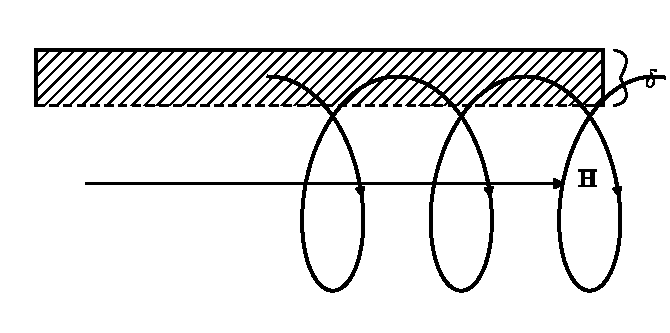
\includegraphics[width=0.72\textwidth]{fig_156.pdf}
\caption*{图 156\quad Azbel'–Kaner 共振。}
\end{figure}
——即速度为 $\mathbf{v}$ 的电子在时刻 $t$ 对 $\mathbf{r}$ 处电流的贡献，取决于场在早先时刻 $t'$ 于电子曾经过的点 $\mathbf{r}'$ 处所给予它的冲量；不过对这个冲量的记忆随时间消退，由一个以弛豫时间 $\tau$ 为特征的衰减因子支配。这种对电传导的描述，在精神上与 Kubo 公式 (7.15) 非常接近。

现在的轨迹是螺旋形的。电子沿一条弯曲路径到达 $\mathbf{r}$，沿这条路径，随时间的衰减仍由同一个指数因子支配。在一个周期内，该因子将为 $\exp(-2\pi/\omega_H\tau)$。电场只在电子处于趋肤深度内的短暂时刻起作用；每回旋一周，电子相对振荡场的相位就将增减一个量 $(2\pi\omega/\omega_H)$。于是，我们可以把式 (9.16) 中的时间积分化为第一次穿过趋肤深度所得的结果，再乘以随后历次穿过的衰减因子之和，即
\begin{equation*}
(1+e^{-w}+e^{-2w}+\ldots)=\frac{1}{1-e^{-w}}, \tag{9.17}
\end{equation*}
其中
\begin{equation*}
e^{-w}=\exp\left(-\frac{2\pi}{\omega_H\tau}-i\,\frac{2\pi\omega}{\omega_H}\right). \tag{9.18}
\end{equation*}
\begin{figure}[H]
\centering
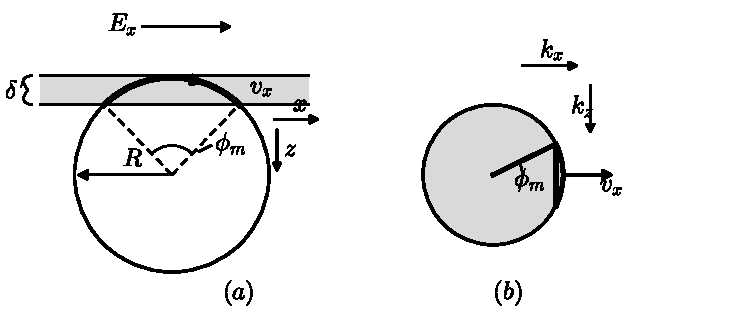
\includegraphics[width=0.72\textwidth]{fig_157.pdf}
\caption*{图 157\quad 电子在角 $\phi_m$ 内是“有效”的：(a) 在真实空间的螺旋路径上；(b) 在费米面上的轨道上。}
\end{figure}
我们可以估计电子的“有效性”：注意到每个电子停留在趋肤深度内的时间只有 $\phi_m/\omega_H$ 的量级，于是（图 157）
\begin{align*}
\phi_m^{2}&\approx\frac{\delta'}{R}\\
&\approx\frac{\delta'\omega_H}{v_x}, \tag{9.19}
\end{align*}
其中 $R$ 是真实空间中轨道的半径，而 $v_x$ 是电子在垂直于磁场的截面平面内、平行于表面方向的速度。

再者，大多数穿过趋肤深度的电子会打到金属表面上，在那里被散射而损失掉。只有在趋肤深度内平行于表面运动的电子才是有效的。用式 (8.107) 中那类论证，我们只计入属于下述费米面元面积的那些电子：
\begin{equation*}
dS=2\beta\phi_m|\rho_y|\,dk_y, \tag{9.20}
\end{equation*}
其中 $\rho_y$ 同样是轨道的曲率半径，取在厚度为 $dk_y$ 的切片上、速度平行于金属表面的那一点处。

把这些论证合在一起，我们得到一个本质上与式 (8.109) 相像的结果，即
\begin{equation*}
\sigma'=\frac{e^{2}\beta\delta'}{2\pi^{3}\hbar}\int\frac{|\rho_y|\,dk_y}{1-e^{-w}}. \tag{9.21}
\end{equation*}
把式 (9.21) 代入式 (8.104) 和式 (8.105)，表面电阻便可算出。

就我们目前的目的而言，有意义的是共振因子 (9.17)。它是振荡的，当
\begin{equation*}
\omega=n\omega_H \tag{9.22}
\end{equation*}
时出现峰值。

实践中，人们保持频率 $\omega$ 不变，而改变磁场。于是，由式 (9.5)，
\begin{equation*}
\frac{1}{H}=n\,\frac{e}{\omega m_H^{*}c} \tag{9.23}
\end{equation*}
就是 $H$ 变化时出现峰值的条件。值得注意的是，Azbel'–Kaner 共振并不像普通回旋共振 (9.14) 那样只有一个单一的峰。只要频率使得电磁场在电子相继两次出现于表面的时刻之间恰好经历整数个振荡周期，能量就仍会被馈入。每个共振的尖锐程度显然取决于式 (9.18) 中 $w$ 的实部的大小；要有强的效应，我们需要 $\omega_H\tau\gg 1$。

还有更进一层的复杂情况。$\omega_H$ 的值（或者等价地，$m_H^{*}$ 的值）依赖于轨道。对于一般的费米面，它在不同的轨道上并\emph{不}相同，即使这些轨道属于垂直于同一磁场的一组平行切片。这样，式 (9.21) 中的变量 $w$ 本身就是 $k_y$ 的函数；来自不同切片的贡献未必保持同相位。

共振曲线形状的精确计算到此变得非常复杂。但人们可以论证——而且这一论证还可以用形式的数学加以支持——主要贡献将来自那些 $m_H^{*}$ 作为 $k_y$ 的函数取平稳值（极大或极小）的截面。如果从每个这样的点出发、把 $m_H^{*}$ 作为 $\delta k_y$ 的函数展开，常数项就提供一个共振峰，而展开式的次一项（$(\delta k_y)^{2}$ 量级）并不能把它消除。来自费米面其他区域——那里 $m_H^{*}$ 随 $\delta k_y$ 线性变化——对积分的贡献则会失去相位而相互抵消。我们遇到的正是波动光学中的惯常论证，那里 Cornu 螺线是对求解很有用的一种几何构图。

\begin{figure}[H]
\centering
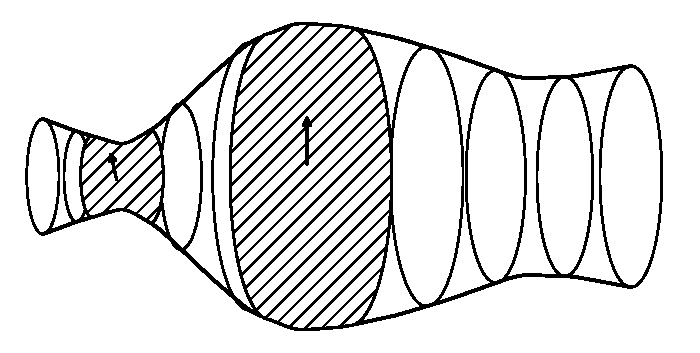
\includegraphics[width=0.72\textwidth]{fig_158.pdf}
\caption*{图 158\quad 极值轨道。}
\end{figure}

\section{强场磁致电阻}

§7.12 中讲述的电流磁效应（galvanomagnetic phenomena）理论，只在载流子位于球形等能面上的情形下才成立。当 $\omega_H\tau>1$ 时，用 $\mathbf{k}$ 的直角坐标分量来表示电子态在数学上变得笨拙，而且由此得到的公式在物理上也难以解释。更简单的做法是直接从以变量 $(\mathcal{E},k_H,\phi)$ 表出的 Boltzmann 方程出发来推导输运性质。我们现在要在恒定电场中寻找稳态解。于是，式 (9.12) 简化为
\begin{equation*}
e\mathbf{E}\cdot\mathbf{v}\left(-\frac{\partial f^{0}}{\partial\mathcal{E}}\right)=\frac{g}{\tau}+\omega_H\frac{\partial g}{\partial\phi}. \tag{9.24}
\end{equation*}
与式 (8.101) 类比，它具有积分
\begin{equation*}
g(\mathcal{E},k_H,\phi)=\frac{e}{\omega_H}\left(-\frac{\partial f^{0}}{\partial\mathcal{E}}\right)\int_{-\infty}^{\phi}\mathbf{v}(\mathcal{E},k_H,\phi)\exp\left\{(\phi''-\phi)/\omega_H\tau\right\}\,d\phi''\cdot\mathbf{E}. \tag{9.25}
\end{equation*}
正如式 (7.27) 那样，可以说费米面在相位角为 $\phi$ 的点处的位移，等于电场在轨道上其他各点所产生的位移的总和；这些位移随后被磁场驱动绕轨道运行，并以特征弛豫时间 $\tau$ 衰减。在低场情形下，衰减如此之快，以致我们只能看到位移方向相对电场方向的一个轻微转动，这正是 Hall 效应的来源（参见式 (7.141)）。

电导率张量现在可以由电流算出：
\begin{align*}
\mathbf{J}&=2\int e\mathbf{v}_{\mathbf{k}}\,g_{\mathbf{k}}\,d\mathbf{k}\\
&=\frac{e}{4\pi^{3}}\iiint \mathbf{v}(\mathcal{E},k_H,\phi)\,g(\mathcal{E},k_H,\phi)\,\frac{m_H^{*}}{\hbar^{2}}\,d\mathcal{E}\,dk_H\,d\phi, \tag{9.26}
\end{align*}
其中我们利用式 (9.7) 和式 (9.8) 来定义 $k_H=$ 常数平面上的一块面积元。代入式 (9.25)，并利用 Fermi 函数导数的性质把积分保持在费米面上，便得到以直角坐标分量表示的电导率张量
\begin{equation*}
\sigma_{\alpha\beta}=\frac{1}{4\pi^{3}}\frac{e^{2}}{\hbar^{2}}\int\frac{m_H^{*}}{\omega_H}\left\{\int_{0}^{2\pi}\int_{0}^{\infty}v_{\alpha}(\phi,k_H)\,v_{\beta}(\phi-\phi',k_H)\,e^{-\phi'/\omega_H\tau}\,d\phi\,d\phi'\right\}dk_H. \tag{9.27}
\end{equation*}
这就是 Shockley 管积分公式（Shockley tube-integral formula）——磁场中电导率张量的一个普适公式。这里对“Kubo 型”表达式（参见式 (7.15)）的这一显式推导相当简单——然而它却是一个威力颇大的公式。

在低场下，我们可以取 $\omega_H\tau\ll 1$，并写出
\begin{equation*}
v_{\beta}(\phi-\phi')=v_{\beta}(\phi)-\phi'\frac{\partial v_{\beta}}{\partial\phi}+\dots, \tag{9.28}
\end{equation*}
因为指数因子使 $\phi'$ 不致变大。显然，$\sigma_{\alpha\beta}$ 中依赖于 $H$ 的各项来自电子速度沿轨道切向的导数，正如式 (7.137) 那样。用这个方法推出我们更熟悉的那些自由电子公式，是一道很好的练习。

在高场下，即 $\omega_H\tau\gg 1$ 时，我们可以利用速度是 $\phi$ 和 $\phi'$ 的周期函数这一事实。$\phi'$ 从 0 到 $\infty$ 的积分范围可以切成若干段，每段长为 $2\pi$。于是
\begin{align*}
\int_{0}^{\infty}e^{-\phi'/\omega_H\tau}f(\phi')\,d\phi'&=\sum_{n}e^{-2\pi n/\omega_H\tau}\int_{0}^{2\pi}e^{-\phi'/\omega_H\tau}f(\phi')\,d\phi'\\
&=\frac{1}{1-e^{-2\pi/\omega_H\tau}}\int_{0}^{2\pi}e^{-\phi'/\omega_H\tau}f(\phi')\,d\phi'\\
&\approx\frac{\omega_H\tau}{2\pi}\int_{0}^{2\pi}e^{-\phi'/\omega_H\tau}f(\phi')\,d\phi'. \tag{9.29}
\end{align*}
在式 (9.27) 中可以消去一个 $\omega_H$ 因子：
\begin{equation*}
\sigma_{\alpha\beta}=\frac{1}{4\pi^{3}}\frac{e^{2}}{\hbar^{2}}\int\frac{m_H^{*}\tau}{2\pi}\left\{\int_{0}^{2\pi}\int_{0}^{2\pi}v_{\alpha}(\phi)\,v_{\beta}(\phi-\phi')\,e^{-\phi'/\omega_H\tau}\,d\phi\,d\phi'\right\}dk_H \tag{9.30}
\end{equation*}
（当然，速度、回旋质量和回旋频率都依赖于 $k_H$，但我们在这里不必显式地写出这一点。）

现在 $\phi'$ 的范围已受限，我们可以对指数函数作展开：
\begin{equation*}
e^{-\phi'/\omega_H\tau}=1-\frac{\phi'}{\omega_H\tau}+\frac{1}{2}\left(\frac{\phi'}{\omega_H\tau}\right)^{2}-\dots. \tag{9.31}
\end{equation*}
式 (9.30) 中的其他函数都与 $\omega_H$ 无关，也就是说与磁场无关。于是，把式 (9.31) 代入式 (9.30)，便给出电导率张量按 $1/H$ 幂次的级数展开。

磁致电阻和 Hall 效应的行为，可以在对 $\sigma$ 的每个分量找出这个展开中第一个不为零的项之后算出。我们将遵循通常的约定，取磁场沿 $z$ 轴。对于首项，由式 (9.8) 有
\begin{align*}
\int v_{x}(\phi')\,d\phi'&=\int v_{\perp}\cos\theta\,\frac{\hbar}{m_H^{*}}\,\frac{dk}{v_{\perp}}\\
&=-\frac{\hbar}{m_H^{*}}\int dk_{y}, \tag{9.32}
\end{align*}
当我们绕闭合轨道一周时，它将为零。

在这种情形下，若 $\alpha$ 或 $\beta$ 中有任何一个指的是垂直于 $\mathbf{H}$ 的平面内的方向，则 $\sigma_{\alpha\beta}$ 中将没有与 $H$ 无关的项。

对于展开中的下一项，我们可以利用式 (9.32) 并作分部积分：
\begin{equation*}
\int_{0}^{2\pi}\phi'\,v_{x}(\phi-\phi')\,d\phi'=\frac{2\pi\hbar}{m_H^{*}}\,k_{y}(\phi)-\frac{\hbar}{m_H^{*}}\int_{0}^{2\pi}k_{y}(\phi-\phi')\,d\phi' \tag{9.33}
\end{equation*}
其中第二项由轨道的中心对称性而为零。但第一项对 $\sigma$ 中支配 Hall 效应的那个分量有贡献：再次利用式 (9.32)，
\begin{align*}
\sigma_{yx}&=\frac{1}{4\pi^{3}}\frac{e^{2}}{\hbar^{2}}\int\frac{m_H^{*}\tau}{2\pi}\,\frac{1}{\omega_H\tau}\int_{0}^{2\pi}v_{y}(\phi)\,\frac{2\pi\hbar}{m_H^{*}}\,k_{y}(\phi)\,d\phi\,dk_{z}\\
&=\frac{1}{4\pi^{3}}e^{2}\int\frac{1}{m_H^{*}\omega_H}\oint k_{y}\,dk_{x}\,dk_{z}\\
&=\frac{ec}{H}\,\frac{1}{4\pi^{3}}\int\mathcal{A}(k_{z})\,dk_{z}, \tag{9.34}
\end{align*}
其中 $\mathcal{A}(k_{z})$ 是 $k_{z}$ 切片上轨道的面积。

\begin{figure}[H]
\centering
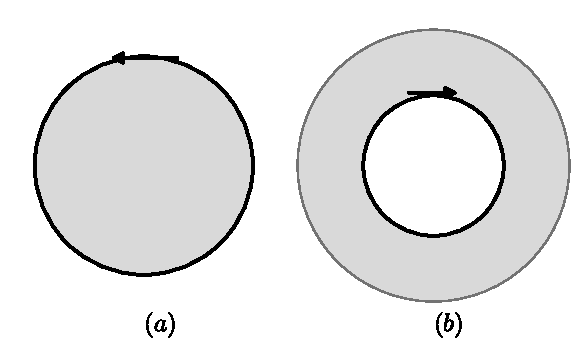
\includegraphics[width=0.72\textwidth]{fig_159.pdf}
\caption*{图 159\quad 在磁场中，代表点绕费米面运动，并使被填充的区域（比如说）保持在左侧。这意味着，对于“电子轨道”(a)，旋转的方向在取向上与“空穴轨道”(b)的相反。}
\end{figure}

这个积分恰好就是被切成轨道的那部分费米面的体积。换言之，
\begin{equation*}
\sigma_{yx}=\frac{ec}{H}\,n, \tag{9.35}
\end{equation*}
其中 $n$ 是被包围在这个费米面之内的电子数。与式 (7.147) 相比较即可看出：在非常强的场中，对任意费米面我们都验证了这个关系。

但如果我们遇到的是一个“空穴”面，情形又会怎样呢？我们必须回头仔细检查整个分析，并注意到沿轨道的绕行方向决定着式 (9.32) 的符号。因此，一个闭合的空穴体积将以相反的符号对式 (9.34) 作出贡献。我们其实应当写成
\begin{equation*}
\sigma_{yx}=\frac{ec}{H}\,(n_{e}-n_{h}). \tag{9.36}
\end{equation*}
这才是对 §7.13 中论证的恰当推广；在高场下，两类载流子的相对迁移率并不进入这一论证。但它只在电子面和空穴面都是闭合面时才适用。

回到式 (9.30) 和式 (9.31)，显而易见，$(1/\omega_H\tau)$ 量级的项在 $\sigma_{xx}$ 和 $\sigma_{yy}$ 中将为零；利用式 (9.32) 和式 (9.33) 极易验证这一点。我们必须用到式 (9.31) 的下一项，即 $(1/\omega_H\tau)^{2}$ 量级的项，才能找到一个不为零的分量。

对 $\sigma$ 的 $z$ 分量，同样的论证也成立。于是 $\sigma_{xz}$ 和 $\sigma_{yz}$ 在一阶下为零，但保留一个 $1/H$ 量级的项；$\sigma_{zz}$ 则含有一个与 $H$ 无关的项。

把这些结果合在一起，我们看到高场下电导率张量的形式如下：——
\begin{equation*}
\boldsymbol{\sigma}=\begin{pmatrix}
\dfrac{A_{xx}}{H^{2}} & \dfrac{-A_{yx}}{H} & \dfrac{-A_{zx}}{H}\\[10pt]
\dfrac{A_{yx}}{H} & \dfrac{A_{yy}}{H^{2}} & \dfrac{-A_{zy}}{H}\\[10pt]
\dfrac{A_{zx}}{H} & \dfrac{A_{zy}}{H} & A_{zz}
\end{pmatrix}, \tag{9.37}
\end{equation*}
其中系数 $A_{xx}$ 等均不为零，且与 $H$ 无关。注意，这个矩阵的非对角元是反对称的：在磁场中，Onsager 关系（§7.9）取如下形式
\begin{equation*}
\sigma_{xy}(\mathbf{H})=\sigma_{yx}(-\mathbf{H}) \tag{9.38}
\end{equation*}
因为坐标轴的反转起到使磁场反转符号的作用。

对这一矩阵的初步考察使人以为，垂直于磁场测得的磁致电阻应当按 $H^{2}$ 无限增大；$\sigma_{xx}$ 难道不是按 $1/H^{2}$ 减小吗？实际情形并非如此，一个初等的论证即可指明。我们的实验是在一根载流导线沿线测量电动势（E.M.F.）。如式 (7.161) 那样，我们必须考察\emph{电阻率张量}的相应分量，它是式 (9.37) 的逆：

例如，让我们考察 $\rho_{xx}$——横向的\emph{电阻率}。由初等矩阵代数，我们有
\begin{align*}
\rho_{xx}&=\frac{1}{\Delta}\left(\frac{A_{yy}A_{zz}+A_{zy}^{2}}{H^{2}}\right)\\
&=\frac{\left(\dfrac{A_{yy}A_{zz}+A_{zy}^{2}}{H^{2}}\right)}{\left(\dfrac{A_{zz}A_{yx}^{2}}{H^{2}}+\dfrac{A_{xx}A_{yy}A_{zz}+A_{xx}A_{zy}^{2}+A_{yy}A_{zx}^{2}}{H^{4}}\right)}\\
&\to\frac{A_{yy}A_{zz}+A_{zy}^{2}}{A_{zz}A_{yx}^{2}} \tag{9.39}
\end{align*}
这里取的是 $1/H$ 的最低次幂。于是，\emph{横向磁致电阻在高场下趋于一个常数}。我们说这个分量\emph{饱和}了。这是 $\boldsymbol{\rho}$ 的所有对角分量的共同特征。在 §7.13 的简单双带模型中我们已经注意到这一现象。

实际发生的是：虽然电导率 $\sigma_{xx}$ 趋于零，这并不意味着不能有电流通过。$x$ 方向的电动势伴随着一个 $y$ 方向的 Hall 电流；为消除这个电流所需的 $y$ 方向电动势又反过来产生一个 $x$ 方向的 Hall 电流，而这正是我们观测到的电流。

对 Hall 系数本身，在同样的极限下我们得到
\begin{equation*}
\rho_{xy}\to\frac{H}{A_{yx}}, \tag{9.40}
\end{equation*}
它与式 (9.36) 联立便给出
\begin{equation*}
R=\frac{1}{(n_{e}-n_{h})ec}. \tag{9.41}
\end{equation*}
在\emph{补偿}金属（compensated metal）的特殊情形——即电子态与空穴态数目相等——这个表达式将变为无穷大。再回过头看式 (9.36)，我们看到 $\sigma_{yx}$ 中的 $1/H$ 线性项消失了：此时电阻率张量的所有分量，包括 Hall 系数本身，都应按磁场的二次幂增大，而不饱和。

\section{开轨道}

在上面的整个论证中，从式 (9.33) 往后，我们都不言自明地假定了所处理的是闭合的等能面——电子的、空穴的，或两者兼有。但这并不是唯一可能的情形。例如，考虑一个

\begin{figure}[H]
\centering
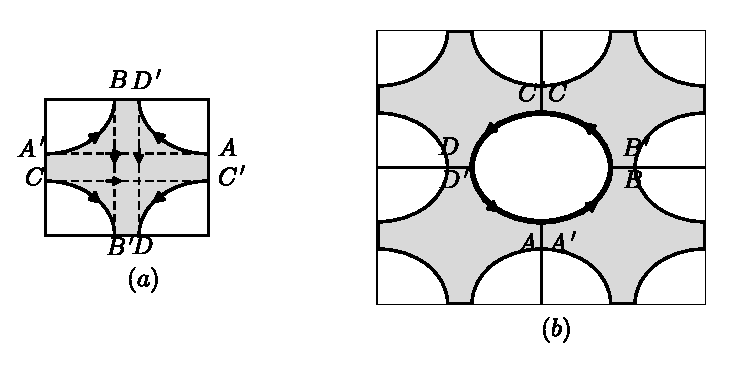
\includegraphics[width=0.72\textwidth]{fig_160.pdf}
\caption*{图 160\quad 轨道：(a) 简约区图式中的；(b) 重复区图式中的。}
\end{figure}

触及区边界的费米面，如图 160(a) 所示。考虑一个从这个平面截面上的 $D'$ 出发的电子，当它到达 $A$ 时会发生什么？如 §3.3 所示，$\mathbf{k}$ 空间中的这个点与平移一个倒格矢后得到的点 $A'$ 等价。代表点从 $A'$ 继续走到 $B$，然后被平移到等价点 $B'$，如此继续下去，依次经过 $C$、$C'$、$D$ 和 $D'$。

这种“轨道”的构造方式显得有些人为，仿佛区边界处存在不连续性似的。但 $A$ 和 $A'$ 确实代表完全相同的波函数。为了把这一点看得更清楚，我们像 §3.3 和 §6.8 中那样画出\emph{重复}区图式。这次我们不再让代表点每次穿过区边界时都平移一个倒格矢，而是在边界的另一侧再提供一个倒格子的晶胞。轨道跨越区边界是连续的，各段如图所示拼接起来。我们应当把它称为\emph{空穴轨道}（hole orbit），因为它围住的是 $\mathbf{k}$ 空间中的一个空区域。它将具有自己特有的回旋频率，正如 §9.1 中那样。

实际上，我们的倒格子是三维的，如图 161 所示。显然，在这种多连通费米面的截面平面上，既可以有电子轨道，也可以有空穴轨道；导致式 (9.36) 的论证必须加以修改。

\begin{figure}[H]
\centering
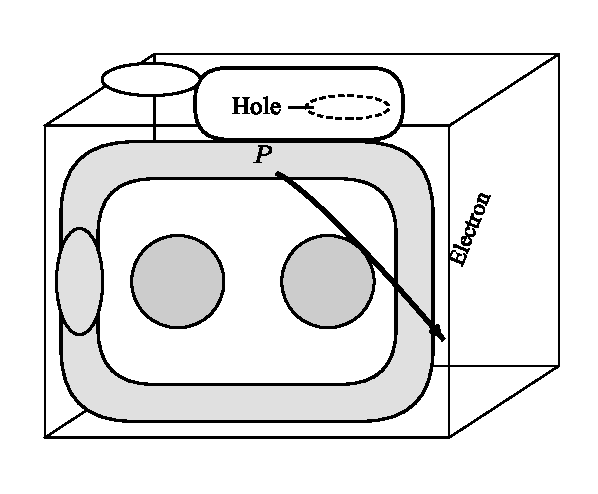
\includegraphics[width=0.72\textwidth]{fig_161.pdf}
\caption*{图 161\quad 在多连通的费米面上，既可以有“电子”轨道，也可以有“空穴”轨道。在诸如 $P$ 这样的点上，一个载流子可以属于两类中的任一类，视磁场方向而定。}
\end{figure}

图 162 表明还有另一种可能。存在这样一个平面，它与费米面的截线不是闭合曲线。此平面内的“轨道”是\emph{开的}（open）。磁场并不能使代表点回到它出发的地方。在重复区图式中，该态的 $\mathbf{k}$ 矢量一直延伸到无穷远。

\begin{figure}[H]
\centering
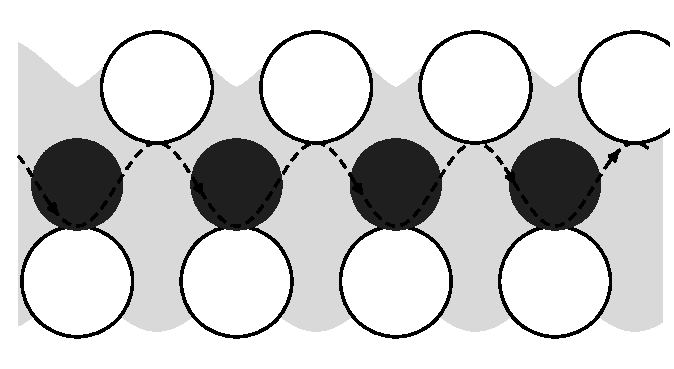
\includegraphics[width=0.72\textwidth]{fig_162.pdf}
\caption*{图 162\quad 一条开轨道。}
\end{figure}

开轨道的存在深刻地改变了上一节的论证。例如，假定存在一条沿 $y$ 方向的开轨道。于是，“积分 (9.32)
\begin{equation*}
\int v_{x}(\phi')\,d\phi'=-\frac{\hbar}{m_H^{*}}\int dk_{y}, \tag{9.42}
\end{equation*}
必定为零”这一证明不再成立。事实上，一眼便可看出，沿这条路径的这个积分的被积函数可能是正定的，因而积分必为有限值。\footnote{严格说来，对于开轨道我们应当重新定义“相位变量”$\phi$。这并没有什么困难；无非是定义一个沿电子在 $\mathbf{k}$ 空间中的路径而变化的变量而已。}这样，$\sigma$ 中凡涉及 $x$ 方向的各个分量都将从这类积分得到贡献；特别地，$\sigma_{xx}$ 将不按 $(1/\omega_H\tau)^{2}$ 变化，而会得出与 $H$ 无关的结果。

再者，这一效应对磁致电阻的影响也必须恰当地加以计算。在式 (9.37) 的位置上我们有
\begin{equation*}
\boldsymbol{\sigma}=\begin{pmatrix}
B_{xx} & \dfrac{-A_{yx}}{H} & -B_{zx}\\[10pt]
\dfrac{A_{yx}}{H} & \dfrac{A_{yy}}{H^{2}} & \dfrac{-A_{zy}}{H}\\[10pt]
B_{zx} & \dfrac{A_{zy}}{H} & A_{zz}
\end{pmatrix} \tag{9.43}
\end{equation*}
作为 $1/H$ 最低阶的各项。于是我们发现 $\rho_{xx}$ 的行为与式 (9.39) 中一样（译注：原文印作“(9.38)”，应为 (9.39)。），趋于饱和；但对电阻率的 $y$ 分量，我们得到
\begin{align*}
\rho_{yy}&=\frac{1}{\Delta}\left(B_{xx}A_{zz}+B_{zx}^{2}\right)\\
&=\frac{B_{xx}A_{zz}+B_{zx}^{2}}{\left\{A_{zz}(A_{yx}^{2}+B_{xx}A_{yy})+B_{xx}A_{yx}^{2}+A_{yy}B_{zx}^{2}\right\}/H^{2}}\\
&\propto H^{2}. \tag{9.44}
\end{align*}
于是，\emph{沿开轨道方向的横向磁致电阻按 $H^{2}$ 增大，而不饱和}。

这一显著现象对费米面的研究十分重要。考察单晶磁致电阻随取向（相对于磁场和电场的方向）的变化，可以提供关于费米面拓扑的证据。例如，如果观察到了不饱和的方向，那么费米面在重复区图式中必定从一个区连通到下一个区；除非电子和空穴的闭合区域体积恰好完全相等，否则它不可能由这些闭合区域构成（参见式 (9.41)）。

图 162 显示了一条典型的开轨道。乍一看，人们会以为所有开轨道都是这种性质，沿着多连通费米面的“轴”走向。于是人们会预期磁致电阻的不饱和方向是晶体的严格对称方向。

实际并非如此，这可以由下面的论证来验证。设一个平面以这样的角度切割一个多连通费米面，使得它既包含闭合的电子轨道，又包含闭合的空穴轨道（图 163）。那么，在包含电子轨道的区域与包含空穴轨道的区域之间，将存在一条开轨道，或者至少一条\emph{扩展轨道}（extended orbit），把这两个区域分隔开。

\begin{figure}[H]
\centering
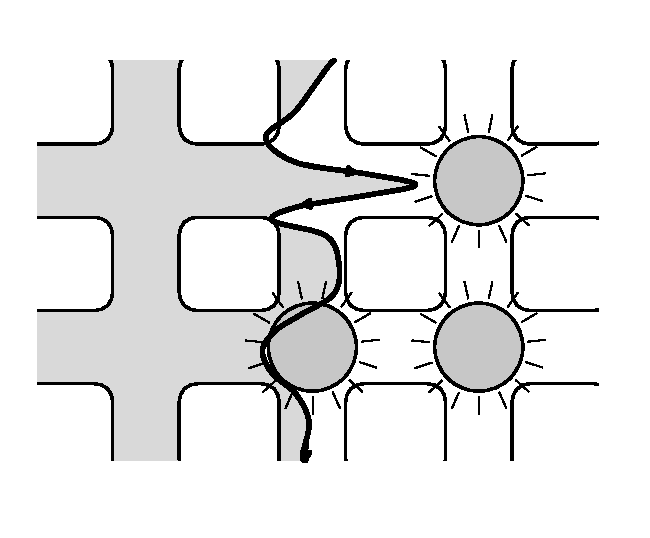
\includegraphics[width=0.72\textwidth]{fig_163.pdf}
\caption*{图 163\quad 分隔“电子”轨道区和“空穴”轨道区的开轨道。}
\end{figure}

这个证明是直观性的。人们无法画出内部带阴影的闭合环路（代表电子轨道）和外部带阴影的闭合环路（代表空穴轨道），而不在阴影区与无阴影区之间补上一条额外的边界。当然，这条边界本身也可能构成一个大的闭合环路——一条\emph{扩展轨道}——但不难构造出这样的情形：它沿着同一大致方向穿过倒格子，无限地延续下去。这一点通过考察简单的模型最易理解。人们发现，这类\emph{非周期}（aperiodic）开轨道常常沿一些方向行进，这些方向围绕对称轴张成相当可观的立体角。在贵金属 Cu、Ag、Au 中情形就是如此，它们的费米面如图 164 中所示。

\section{磁声振荡}

正如我们在 §8.8 中看到的，超声波的衰减并不能直接给出费米面形状的量度。但是，如果在施加超声波的同时加上磁场，就会观察到一些确实直接依赖于表面几何结构的现象。

这些现象无论在理论上还是在实践上都极其复杂；磁场方向、超声波的传播矢量
\begin{figure}[H]
\centering
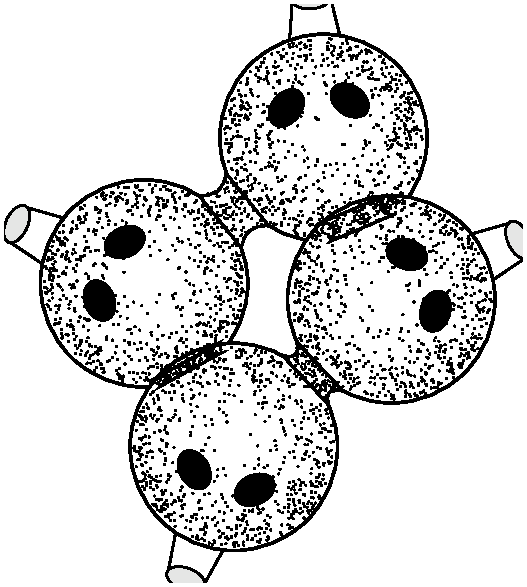
\includegraphics[width=0.72\textwidth]{fig_164.pdf}
\caption*{图 164\quad 铜的费米面。}
\end{figure}
以及波的偏振矢量，可以排布的方式实在太多。为了作完整的分析，人们必须构造一个广义电导率 $\boldsymbol{\sigma}(\mathbf{q},\omega)$，它类似于式 (8.115)，但像式 (9.14) 或式 (9.21) 中那样以回旋坐标表出。这是可以做到的——但不可避免地会被问题的几何格局弄得相当繁复。

不过，下面的简单例子可以说明这个效应。设磁场沿 $z$ 方向，另有一个横超声波，其偏振矢量沿 $y$ 方向，沿 $x$ 方向传播。考虑一个电子在真实空间中的实际路径。对自由电子而言，这将是一条螺旋线，也就是投射在 $(x,y)$ 平面上的一个圆。对于 $\mathbf{k}$ 空间中的“轨道”，这个投影很容易确定。一般地，
\begin{equation*}
\mathbf{k}=\frac{e}{c\hbar}\,\mathbf{H}\wedge\dot{\mathbf{r}}, \tag{9.45}
\end{equation*}
正如式 (6.40) 那样。由此，经一次初等的时间积分即得
\begin{equation*}
\mathbf{k}=\frac{e}{c\hbar}\,\mathbf{H}\wedge\mathbf{r}. \tag{9.46}
\end{equation*}
$\mathbf{k}$ 在 $\mathbf{k}$ 空间中的轨道，与 $\mathbf{r}$ 在真实空间中的路径的 $x$-$y$ 投影相同，只是要乘以 $eH/c\hbar$，并绕 $\mathbf{H}$ 旋转一个直角。

\begin{figure}[H]
\centering
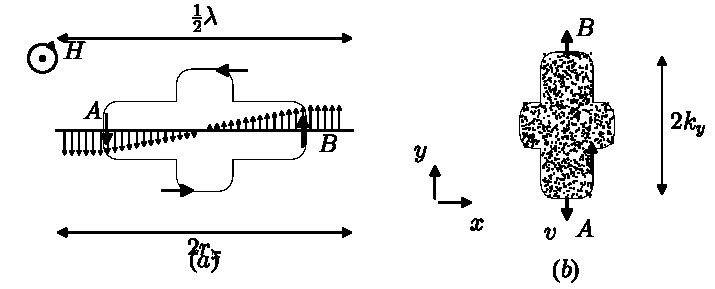
\includegraphics[width=0.72\textwidth]{fig_165.pdf}
\caption*{图 165\quad (a) 电子在真实空间中的轨迹；(b) 费米面上的轨道。}
\end{figure}

现在考虑由声波建立的电场。对一切实用目的而言，我们可以把它当作一个垂直于传播方向的静态振荡电场。实际上，为使 $\omega_H\tau\gg 1$，我们需要一个强到 $\omega_H\gg\omega$ 的磁场；电子在被散射之前、或者在电场发生变化之前，要绕轨道转许多圈。于是，重要的因素是电子沿路径绕行时所见到的电场变化。从图 165 显然可以看出，可以把这个电场安排成：在 $\mathbf{E}$ 与 $\mathbf{v}$ 平行的两个点上，它都使电子沿轨道向同一转向加速。这是一种\emph{几何共振}（geometrical resonance）；显然，条件是回路的直径应当是场的半波长的奇数倍：
\begin{equation*}
2r_{x}=\frac{\hbar c}{eH}\,2k_{y}=\left(n+\frac{1}{2}\right)\lambda. \tag{9.47}
\end{equation*}
对于固定的波长，当 $H$ 变化时，吸收将以 $1/H$ 的一个确定周期而振荡。这个周期应当给出费米面的直径——在电子速度平行于声波所产生的电矢量的那些点之间量得的直径。

然而，这个共振条件 (9.47) 并不十分精确。只要考察圆形轨道的情形就可以看出这一点。例如，设
\begin{equation*}
v_{y}(t)=v_{0}\sin\omega_H t, \tag{9.48}
\end{equation*}
且有
\begin{equation*}
x(t)=r_{x}\sin\omega_H t, \tag{9.49}
\end{equation*}
那么，在 $E_{y}\exp(iqx)$ 的场中，每周期吸收的能量将为
\begin{align*}
\int\mathbf{E}\cdot\mathbf{v}\,dt&=E_{y}v_{0}\int_{0}^{2\pi/\omega_H}\exp(iqr_{x}\sin\omega_H t)\sin\omega_H t\,dt\\
&=\frac{E_{y}v_{0}}{\omega_H}\int_{0}^{2\pi}\exp(iqr_{x}\sin\xi)\sin\xi\,d\xi\\
&=\frac{E_{y}v_{0}}{\omega_H}\,2\pi J_{1}(qr_{x}). \tag{9.50}
\end{align*}
于是，“共振”将出现在 Bessel 函数 $J_{1}(qr_{x})$ 的极大值处。在式 (9.47) 中的 $(n+\frac{1}{2})$ 的位置上，我们得到的是 1.22、2.23、3.24…$(n+\frac{1}{4})$ 这样的数。因此，在解释这一效应时必须谨慎。此外，弹性波的应变场与电子所受力之间的关系也会进入计算，并影响共振的位置。

\begin{figure}[H]
\centering
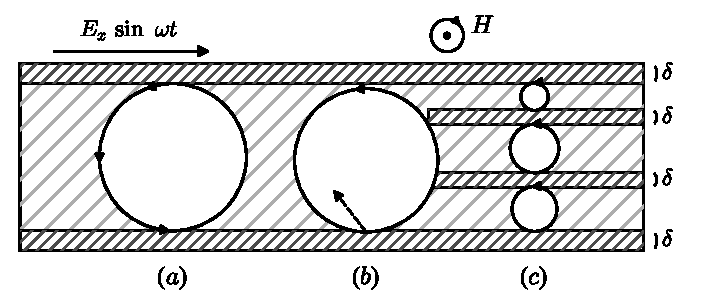
\includegraphics[width=0.72\textwidth]{fig_166.pdf}
\caption*{图 166\quad 射频尺寸效应：(a) 极值轨迹；(b) 被散射的轨迹；(c) 由内部趋肤层诱导的轨迹链。}
\end{figure}

一组电子轨道的卡钳直径还可以用更直接的方法测定，这就是 Gantmakher 效应，或称\emph{射频尺寸效应}（r.f. size effect）。在任意射频 $\omega\ll\omega_H$ 下，测量一块非常纯的金属薄片，且磁场平行于其表面时的表面阻抗。在趋肤深度中被加速的一个电子沿一条闭合轨迹
，其直径随 $H$ 的减小而增大。当这条轨道大到一定程度时，电子就会撞到薄片的下表面而被散射。表面阻抗对“有效”电子（§§ 8.7、9.2）颇为敏感，当式 (9.47) 中的 $2r_{x}$ 等于样品厚度时就会改变（图 166）。

这一现象完全没有利用回旋共振条件；而且由于表面是名副其实的空间不连续处，它比磁声效应更为明锐。但我们同样观察到在 $1/H$ 下具有恒定周期的振荡，来自各组极值轨道的贡献之间还发生干涉。这是因为，从薄片顶面趋肤深度出发的有效电子，会在顶面下方卡钳直径处汇合成一个薄薄的电流层。这个新的“趋肤层”又充当另一组轨道的源——如此等等。如果这样一条轨道链恰好能塞进薄片的厚度，从而在下表面产生一个“趋肤深度”区，样品对射频场就会显得比我们预料的透明得多。可是一旦下端轨道上的电子碰到这个表面，阻抗便急剧改变。再加上把不同的极值轨道组组合起来的种种可能性，观测结果变得相当复杂。不过，这些以及类似的非共振\emph{磁形态学}（magnetomorphic）现象，能够给出有关费米面的大量细致信息。

\section{轨道的量子化}

回旋频率 $\omega_{H}$ 就好比简谐振子的频率。因此我们预期会看到能量以 $\hbar\omega_{H}$ 为单位量子化。事实确实如此——尽管一个完全普遍的证明至今尚未给出。

但来考虑磁场中的自由电子。它们满足薛定谔方程
\begin{equation*}
\frac{1}{2m}\left(\frac{\hbar}{i}\nabla-\frac{e}{c}\mathbf{A}\right)^{2}\psi=\mathcal{E}\psi,
\tag{9.51}
\end{equation*}
其中 $\mathbf{A}$ 是矢势。我们要求出这个系统的定态。选取规范
\begin{equation*}
\mathbf{A}=(0,Hx,0),
\tag{9.52}
\end{equation*}
其旋度给出沿 $z$ 方向的场 $H$。

把式 (9.52) 代入式 (9.51)，我们必须求解
\begin{equation*}
\frac{\partial^{2}\psi}{\partial x^{2}}+\left(\frac{\partial}{\partial y}-\frac{ieH}{\hbar c}x\right)^{2}\psi+\frac{\partial^{2}\psi}{\partial z^{2}}+\frac{2m\mathcal{E}}{\hbar^{2}}\psi=0.
\tag{9.53}
\end{equation*}
这显然具有如下形式的解：
\begin{equation*}
\psi(x,y,z)=\exp\left\{i(\beta y+k_{z}z)\right\}u(x),
\tag{9.54}
\end{equation*}
其中 $u(x)$ 须满足方程
\begin{equation*}
\frac{\partial^{2}u}{\partial x^{2}}+\left\{\frac{2m\mathcal{E}'}{\hbar^{2}}-\left(\beta-\frac{eH}{\hbar c}x\right)^{2}\right\}u=0,
\tag{9.55}
\end{equation*}
其中
\begin{equation*}
\mathcal{E}'=\mathcal{E}-\frac{\hbar^{2}}{2m}k_{z}^{2}.
\tag{9.56}
\end{equation*}

沿 $z$ 方向——也就是平行于场的方向——的运动与自由电子完全相同，它对动能的贡献也一样。但对于 $(x,y)$ 平面内的运动，我们必须求解一个新的本征值方程 (9.55)，它可以写成
\begin{equation*}
-\frac{\hbar^{2}}{2m}\frac{\partial^{2}u(x)}{\partial x^{2}}+\frac{1}{2}m\left(\frac{eH}{mc}x-\frac{\hbar\beta}{m}\right)^{2}u(x)=\mathcal{E}'u(x).
\tag{9.57}
\end{equation*}
这不外乎就是简谐振子的波函数 $u(x)$ 的一维薛定谔方程，振子频率为
\begin{equation*}
\omega_{H}=\frac{eH}{mc},
\tag{9.58}
\end{equation*}
中心位于点
\begin{equation*}
x_{0}=\frac{1}{\omega_{H}}\frac{\hbar\beta}{m}.
\tag{9.59}
\end{equation*}
于是，
\begin{equation*}
\mathcal{E}'=\left(n+\frac{1}{2}\right)\hbar\omega_{H},
\tag{9.60}
\end{equation*}
而
\begin{equation*}
\mathcal{E}=\left(n+\frac{1}{2}\right)\hbar\omega_{H}+\frac{\hbar^{2}}{2m}k_{z}^{2}.
\tag{9.61}
\end{equation*}

这正是我们想要的结果：电子态的能量表为沿磁场方向的平移动能，加上垂直于磁场的平面内回旋运动的量子化能量之和。

有趣的问题是——我们怎样数状态？设有一个盒子，如 §1.7 中那样，边长为 $L_{x}$、$L_{y}$、$L_{z}$。显然，$k_{z}$ 像通常一样以 $2\pi/L_{z}$ 为单位量子化。同样，由式 (9.54) 的形式，$\beta$ 以 $2\pi/L_{y}$ 为单位量子化。但要注意，能量与 $\beta$ 无关，因此人们或许以为，对给定的 $n$，$\beta$ 可以取自一个无限集合中的任何值。

但情况并非如此。如式 (9.59) 所示，函数 $u$ 对 $\beta$ 的依赖体现在它以某点为中心：
\begin{equation*}
x_{0}=\frac{1}{\omega_{H}}\frac{\hbar\beta}{m}=\frac{v_{y}}{\omega_{H}}.
\tag{9.62}
\end{equation*}
这实际上意味着：如果电子以速度 $v_{y}$ 沿 $y$ 方向出发，它将在磁场中走一条圆形路径，圆心为 $x_{0}$。这条路径不能太大。$x_{0}$ 必须落在盒子之内，于是有
\begin{equation*}
0<x_{0}<L_{x}
\tag{9.63}
\end{equation*}
作为对这一中心允许位置的限制。

\begin{figure}[H]
\centering
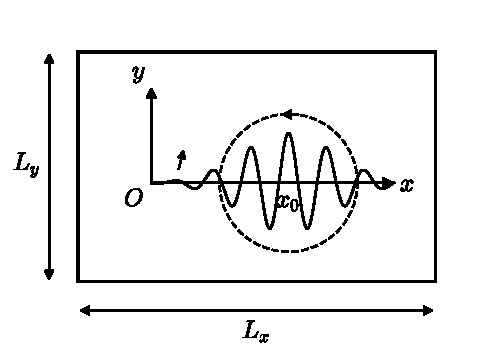
\includegraphics[width=0.72\textwidth]{fig_167.pdf}
\caption*{图 167\quad 磁场中电子薛定谔方程的解。}
\end{figure}

但由式 (9.62)，这就限制了 $\beta$ 的允许取值范围。这个变量不仅以 $2\pi/L_{y}$ 为单位量子化，而且还必须满足
\begin{equation*}
0<\beta<\frac{m\omega_{H}}{\hbar}L_{x}=\frac{eH}{c\hbar}L_{x}.
\tag{9.64}
\end{equation*}
因此，只有
\begin{equation*}
p=\frac{L_{y}}{2\pi}\frac{m\omega_{H}}{\hbar}L_{x}
\tag{9.65}
\end{equation*}
个不同的 $\beta$ 值。式 (9.61) 的每个能级，对应于 $n$ 和 $k_{z}$ 的一种特定选择，是 $p$ 重简并的。

磁场当然已经破坏了我们原先的量子化图式。变量 $k_{x}$、$k_{y}$、$k_{z}$ 曾是我们在 k 空间中的坐标，如今不再是“好量子数”；波函数 (9.54) 也不再各自对应于这组参数的一组固定取值。尽管如此，让我们仍用这同一空间，并且把具有式 (9.61) 所给的某个 $\mathcal{E}$ 值的 $p$ 个新能级，用我们原图式中对应此能量的等能面来表示。略去 $z$ 坐标，这些面便是 $(k_{x},k_{y})$ 平面中的圆（译注：原文印作“$(x,y)$ 平面”。）。新的状态其实并不定域于圆上任何一点；它们将绕着圆以频率 $\omega_{H}$ 转动。但我们可以通过指明各能级所在的圆，来对磁场中的各个能级进行分类。

\begin{figure}[H]
\centering
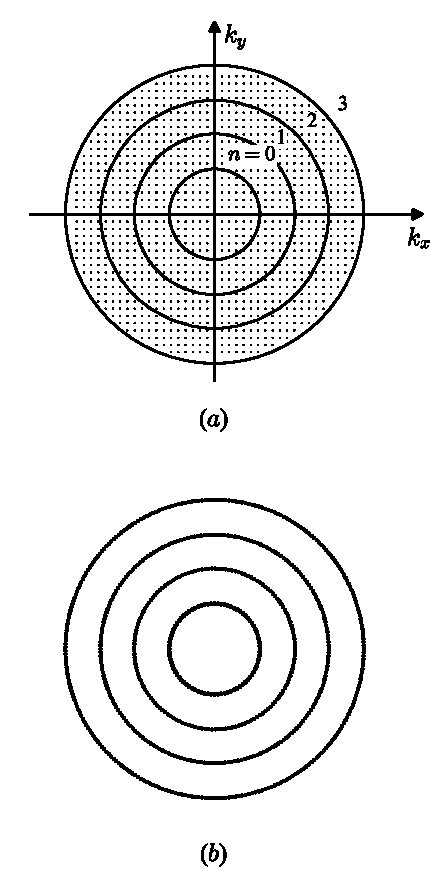
\includegraphics[width=0.72\textwidth]{fig_168.pdf}
\caption*{图 168\quad 自由电子的量子化图式：(a) 无磁场时；(b) 有磁场时。}
\end{figure}

\emph{事实上我们可以核验：与 k 空间中任一给定宏观体积相联系的能级总数，在新图式中与原先相同。}我们可以利用式 (9.7)；相隔能量 $\delta\mathcal{E}$ 的两个等能面之间的面积为
\begin{equation*}
\delta\mathcal{A}=\frac{2\pi m_{H}^{*}}{\hbar^{2}}\delta\mathcal{E}.
\tag{9.66}
\end{equation*}
设 $\delta\mathcal{E}$ 是回旋频率的一个量子 $\hbar\omega_{H}$。回想在常规量子化图式中，“允许状态”的密度是每单位 $(k_{x},k_{y})$ 平面面积 $(L_{x}L_{y})/(2\pi)^{2}$（参见 §1.6）。于是，两条量子化轨道之间的状态数为
\begin{align*}
\frac{L_{x}L_{y}}{(2\pi)^{2}}\delta\mathcal{A}&=\frac{2\pi m_{H}^{*}}{\hbar^{2}}\hbar\omega_{H}\frac{L_{x}L_{y}}{(2\pi)^{2}}\\
&=p
\tag{9.67}
\end{align*}
即式 (9.65)。

这正是我们想要的结果。它表明，磁场的效应可以说是在 k 空间中造就出这些量子化轨道，并使自由电子状态“凝聚”到最近的一条这样的轨道上。每条轨道上的状态数，恰好等于它所处的那个环带内“允许状态”的数目。

那么，当我们处理的是晶体中的电子时，一般情形又会怎样？对单个能带，§6.5 的准经典理论有效。等效哈密顿量的薛定谔方程 (6.30) 在磁场中的解，在大量子数下将满足对应原理极限，并将按 Bohr 相位积分公式量子化：
\begin{equation*}
\oint\mathbf{p}\cdot d\mathbf{r}=(n+\gamma)\,2\pi\hbar,
\tag{9.68}
\end{equation*}
其中 $n$ 是整数，$\gamma$ 是相位修正（典型值为 $\frac{1}{2}$），$\mathbf{p}$ 和 $\mathbf{r}$ 是共轭变量，表示粒子描出其轨道时的动量和位置。

我们可以利用式 (9.45) 来计算 $\mathbf{r}$，即电子在真实空间中沿其路径的位置；并且可以采用通常的动量规则
\begin{equation*}
\mathbf{p}=\hbar\mathbf{k}+\frac{e}{c}\mathbf{A}.
\tag{9.69}
\end{equation*}
由简单的几何推理即得：\emph{轨道在 k 空间中的面积是量子化的}：
\begin{equation*}
\mathcal{A}_{n}=\frac{2\pi eH}{c\hbar}(n+\gamma).
\tag{9.70}
\end{equation*}
由式 (9.61)、(9.66) 和 (9.5) 显然可见，这正是前面已对自由电子得到的结果。

要在磁场中描述电子能级，现在需要在 k 空间中作如下构造。选定一个 $n$ 值。在费米面每个垂直于磁场的截面上，画出面积为 $\mathcal{A}_{n}$ 的等能围线。把这些围线连成一根连续的管子，其轴平行于 $H$，且横截面积处处相同。对其余的 $n$ 值同样画出管子。假定常规量子化图式中的“允许点”已全部凝聚到最近的管子上。这就给出了在能量上简并的状态数，它们现在应被想象成以各自轨道相应的回旋频率绕每根管子环流。

\begin{figure}[H]
\centering
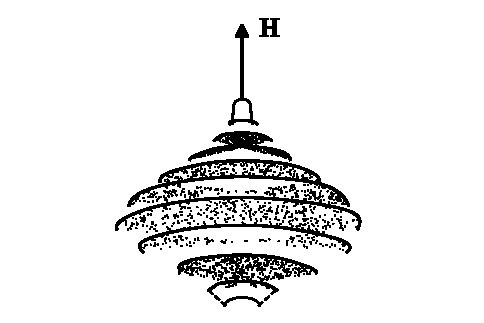
\includegraphics[width=0.72\textwidth]{fig_169.pdf}
\caption*{图 169\quad 量子化磁能级的管。}
\end{figure}

\section{de Haas--van Alphen 效应}

这种量子化有一些有趣而惊人的效应。电子气体作为一个整体的能量依赖于磁场的强度。而磁化率——它基本上是抗磁性的（这里我们忽略自旋效应），并且与温度无关——却随着磁场的改变而振荡。这就是 de Haas--van Alphen 效应。

要对一般形状的费米面计算这个效应，我们可以按如下步骤进行。先写下系统的自由能；对 Fermi--Dirac 系集（assembly），它由下式给出：
\begin{equation*}
F=N\zeta-kT\sum_{i}\ln\left(1+e^{(\zeta-\mathcal{E}_{i})/kT}\right),
\tag{9.71}
\end{equation*}
其中对所有可能的状态求和，状态能量为 $\mathcal{E}_{i}$；但我们由被占据状态的数目来固定 $\zeta$，即 Fermi 势（例如如式 (4.9) 中那样）。

对我们的量子化 \emph{Landau 能级}系统，能量由下式给出：
\begin{equation*}
\mathcal{E}_{i}=\mathcal{E}(n+\gamma,k_{z}),
\tag{9.72}
\end{equation*}
其中 $n$ 是轨道量子数，如式 (9.61) 中那样——但当然，如式 (9.65) 那样，每个这样的能级是 $p$ 重简并的。取一块单位边长的晶体立方；按式 (9.67) 或 (9.70)，k 空间中每根管子长度为 $dk_{z}$（照常沿 $H$ 方向量度）的一段上将有
\begin{equation*}
\frac{1}{4\pi^{3}}d^{3}k=\frac{eH}{2\pi^{2}\hbar c}\,dk_{z}
\tag{9.73}
\end{equation*}
个状态属于它。于是
\begin{equation*}
F=N\zeta-kT\int_{-\infty}^{\infty}\left\{\frac{eH}{2\pi^{2}\hbar c}\sum_{n=0}^{\infty}\ln\left(1+\exp\left[\left\{\zeta-\mathcal{E}(n+\gamma,k_{z})\right\}/kT\right]\right)\right\}dk_{z}.
\tag{9.74}
\end{equation*}

要算这个讨厌的积分，我们用一招纯数学的技巧——Poisson 求和公式。考虑 $f(x)$，一个任意函数。在 $n<x<n+1$ 范围内可以写成
\begin{equation*}
f(x)=\sum_{s=-\infty}^{\infty}e^{-2\pi ixs}g_{s},
\tag{9.75}
\end{equation*}
其中
\begin{equation*}
g_{s}=\int_{n}^{n+1}f(x)\,e^{2\pi ixs}dx.
\tag{9.76}
\end{equation*}
这正是一个 Fourier 级数，如式 (1.7)。于是可以写
\begin{align*}
f\left(n+\frac{1}{2}\right)&=\sum_{s=-\infty}^{\infty}e^{-2\pi is(n+\frac{1}{2})}g_{s}\\
&=\sum_{s=-\infty}^{\infty}e^{-i\pi s}g_{s}\\
&=\sum_{s=-\infty}^{\infty}(-1)^{s}\int_{n}^{n+1}f(x)\,e^{2\pi ixs}dx.
\tag{9.77}
\end{align*}
现在把上式对变量 $x$ 的所有区间求和，得
\begin{equation*}
\sum_{n=0}^{\infty}f\left(n+\frac{1}{2}\right)=\int_{0}^{\infty}f(x)\,dx+2\sum_{s=1}^{\infty}(-1)^{s}\int_{0}^{\infty}f(x)\cos 2\pi xs\,dx.
\tag{9.78}
\end{equation*}
我们把这个公式用到式 (9.74) 中对 $n$ 的求和上：
\begin{align*}
F&=N\zeta-kT\int_{-\infty}^{\infty}\left\{\frac{eH}{2\pi^{2}\hbar c}\int_{0}^{\infty}\ln\left(1+\exp\left[\left\{\zeta-\mathcal{E}(x+\gamma,k_{z})\right\}/kT\right]\right)dx\right\}dk_{z}\\
&\quad-2kT\sum_{s=1}^{\infty}\int_{-\infty}^{\infty}\left\{\frac{eH}{2\pi^{2}\hbar c}(-1)^{s}\int_{0}^{\infty}\ln\left(1+\exp\left[\left\{\zeta-\mathcal{E}(x+\gamma,k_{z})\right\}/kT\right]\right)\right.\\
&\qquad\left.\times\cos 2\pi xs\,dx\right\}dk_{z}.
\tag{9.79}
\end{align*}

我们暂且把注意力集中于如下形式的积分：
\begin{align*}
&\int_{0}^{\infty}\ln\left(1+\exp\left[\left\{\zeta-\mathcal{E}(x+\gamma,k_{z})\right\}/kT\right]\right)\cos 2\pi xs\,dx\\
&\quad=\frac{1}{4\pi^{2}s^{2}kT}\left[f^{0}(\mathcal{E})\frac{\partial\mathcal{E}}{\partial x}\right]_{x=0}+\int_{0}^{\infty}\frac{\cos 2\pi xs}{4\pi^{2}s^{2}kT}\left[f^{0}(\mathcal{E})\frac{\partial^{2}\mathcal{E}}{\partial x^{2}}+\frac{\partial f^{0}}{\partial x}\frac{\partial\mathcal{E}}{\partial x}\right]dx.
\tag{9.80}
\end{align*}
这里我们用到了
\begin{equation*}
kT\,\frac{\partial\ln\left(1+e^{(\zeta-\mathcal{E})/kT}\right)}{\partial\mathcal{E}}=f^{0}(\mathcal{E}),
\tag{9.81}
\end{equation*}
即式 (4.8) 所定义的 Fermi 函数，并且已分部积分两次。我们将略去式 (9.80) 中的第一项，因为我们只关心自由能的振荡部分。利用式 (9.61)，按定义有
\begin{equation*}
\mathcal{E}(x+\gamma,k_{z})=(x+\gamma)\hbar\omega_{H}+f(k_{z}),
\tag{9.82}
\end{equation*}
于是 $\partial\mathcal{E}/\partial x=\hbar\omega_{H}$，而 $\partial^{2}\mathcal{E}/\partial x^{2}=0$。再者，积分下限不妨取 $-\infty$，因为对积分的重要贡献只来自费米能级 $\mathcal{E}=\zeta$ 附近。于是，费米分布的这一薄层对自由能的贡献正比于
\begin{equation*}
I_{s}(k_{z})=\frac{\hbar\omega_{H}(\zeta,k_{z})}{4\pi^{2}s^{2}kT}\int_{-\infty}^{\infty}\cos 2\pi xs\,\frac{\partial f^{0}}{\partial x}\,dx.
\tag{9.83}
\end{equation*}

这个积分虽然名义上具有式 (4.13) 的形式，却不能用那个公式求值，因为被积函数在 Fermi 层厚度之内振荡得太快。但我们可以利用这样一个事实：$-\partial f^{0}/\partial x$ 在点 $X$ 处取极大，$X$ 满足
\begin{equation*}
\mathcal{E}(X,k_{z})=\zeta:
\tag{9.84}
\end{equation*}
我们可以说
\begin{equation*}
X=\frac{c\hbar}{2\pi eH}\,\mathcal{A}(\zeta,k_{z}),
\tag{9.85}
\end{equation*}
其中 $\mathcal{A}(\zeta,k_{z})$ 是费米面在切片 $k_{z}$ 处、实际费米能级上的横截面面积。我们把积分在这个点附近展开——记住 $\partial f^{0}/\partial x$ 是 $x$ 的偶函数——便得
\begin{align*}
I_{s}(k_{z})&\approx\frac{\hbar\omega_{H}}{4\pi^{2}s^{2}kT}\int_{-\infty}^{\infty}\cos 2\pi s\left(X+\frac{kT}{\hbar\omega_{H}}\eta\right)\frac{\partial f^{0}}{\partial\eta}\,d\eta\\
&=\frac{\hbar\omega_{H}}{4\pi^{2}s^{2}kT}\cos 2\pi sX\int_{-\infty}^{\infty}\cos\left(\frac{2\pi skT}{\hbar\omega_{H}}\eta\right)\frac{\partial f^{0}}{\partial\eta}\,d\eta\\
&=-\frac{\hbar\omega_{H}}{4\pi^{2}s^{2}kT}\cos\left(\frac{sc\hbar\mathcal{A}(\zeta,k_{z})}{eH}\right)\left\{\frac{2\pi^{2}skT/\hbar\omega_{H}}{\sinh\left(2\pi^{2}skT/\hbar\omega_{H}\right)}\right\}\\
&=-g(s,k_{z})\cos\left(\frac{sc\hbar\mathcal{A}(\zeta,k_{z})}{eH}\right),\quad\text{姑且记之。}
\tag{9.86}
\end{align*}

写到这里，我们或许应该停下来喘口气，看看究竟发生了什么。我们考虑的是费米面的一个特定切片。由整个图形的体积所固定的费米能级，未必恰好与某条量子化磁轨道重合。随着场的改变，量子化轨道被拉进、拉出，扫过费米能级，如图 170 所示。

\begin{figure}[H]
\centering
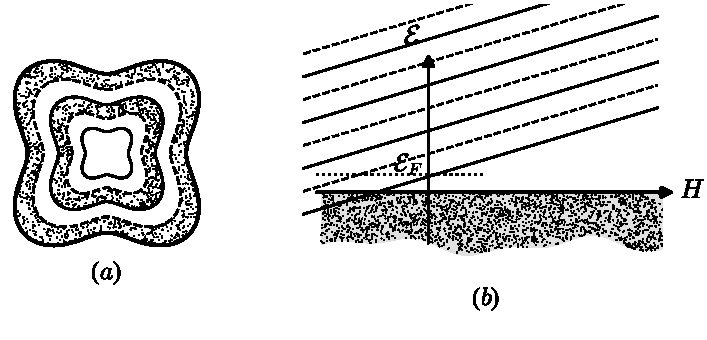
\includegraphics[width=0.72\textwidth]{fig_170.pdf}
\caption*{图 170\quad (a) 费米面未必与量子化轨道重合。(b) 磁场改变时，量子化能级扫过费米能级。}
\end{figure}

\begin{figure}[H]
\centering
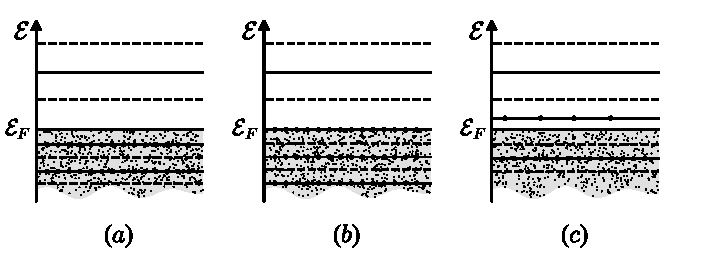
\includegraphics[width=0.72\textwidth]{fig_171.pdf}
\caption*{图 171\quad 磁场改变时磁能级的占据情况。}
\end{figure}

设我们处于 $T=0$，费米分布完全锐利。当一条量子化轨道扫过 $\zeta$ 时会发生什么？例如，设场的大小恰使 $\zeta$ 位于两条轨道的正中间（图 171(a)）。这时费米能级以下的状态数，与完全没有磁能级时的情形一模一样——但电子气体的总能量将低于没有磁场时的值——费米能级上每个电子约低 $\frac{1}{2}\hbar\omega_{H}$ 的量级。现在，随着 $H$ 增大，这些电子将被拉向费米能级（图 171(b)），其自由能随之升到一个极大。而当磁能级穿过费米能级时，它开始倒空（图 171(c)），电子的平均能量再度下降，并在 $\zeta$ 再次位于两条量子化轨道正中间时达到极小。这样，电子气体的自由能便规则地振荡，其周期由量子化轨道与费米能级相邻两次重合的间隔决定。这就是式 (9.86) 的含义；周期来自条件
\begin{equation*}
\frac{sc\hbar\mathcal{A}(\zeta,k_{z})}{eH}=2n\pi.
\tag{9.87}
\end{equation*}

从式 (9.74) 到式 (9.81) 的大部分代数演算，都是为把振荡按 Fourier 级数来分析而设的手段，因为每个能级扫过费米面时能量的变化并不是简单的正弦函数。这也解释了指标 $s$ 的由来——它给出更高的谐波。

我们也已经考虑到 $T\neq 0$ 时费米面并非完全锐利这一事实；事实上，若
\begin{equation*}
kT\gg\hbar\omega_{H},
\tag{9.88}
\end{equation*}
则所有振荡都将被抹平。换句话说，磁场必须强到使轨道的间距达到费米面上热层厚度的量级。

但分析到此还没有完结。以上只是对 $k_{z}$ 处一个特定截面的计算；我们必须对所有不同的切片求和：
\begin{equation*}
F=2kT\sum_{s=1}^{\infty}(-1)^{s}\int_{-\infty}^{\infty}\frac{eH}{2\pi^{2}\hbar c}\,g(s,k_{z})\cos\left(\frac{sc\hbar\mathcal{A}(\zeta,k_{z})}{eH}\right)dk_{z}.
\tag{9.89}
\end{equation*}
这是一个 Fresnel 型积分；众所周知，主要贡献来自相位驻定的区域。设
\begin{equation*}
\frac{\partial\mathcal{A}(\zeta,k_{z})}{\partial k_{z}}=0
\tag{9.90}
\end{equation*}
在 $k_{z}=k_{0}$ 处成立。在该点附近展开：$k_{z}=k_{0}+k'$，且
\begin{equation*}
\mathcal{A}=\mathcal{A}_{0}\pm\frac{1}{2}k'^{2}\mathcal{A}_{0}''\dots
\tag{9.91}
\end{equation*}
（$g(s,k_{z})$ 的变化可以忽略——而且我们也不言自明地假定了费米面的每一部分都有一个对称中心。）于是
\begin{align*}
F&=2kT\sum_{s=1}^{\infty}(-1)^{s}\frac{eH}{2\pi^{2}\hbar c}\,g(s,k_{0})\int_{-\infty}^{\infty}\cos\left\{\frac{sc\hbar}{eH}\left(\mathcal{A}_{0}\pm\frac{1}{2}k'^{2}\mathcal{A}_{0}''\dots\right)\right\}dk'\\
&\approx 2kT\sum_{s=1}^{\infty}(-1)^{s}\left(\frac{eH}{2\pi^{2}\hbar c}\right)g(s,k_{0})\left(\frac{2eH}{sc\hbar|\mathcal{A}_{0}''|}\right)^{\frac{1}{2}}\cos\left(\frac{sc\hbar\mathcal{A}_{0}}{eH}\pm\frac{\pi}{4}\right)\\
&=2kT\sum_{s=1}^{\infty}(-1)^{s}\left(\frac{eH}{2\pi sc\hbar}\right)^{\frac{1}{2}}\frac{1}{\sinh\left(2\pi^{2}skT/\hbar\omega_{H}\right)}\,|\mathcal{A}_{0}''|^{-\frac{1}{2}}\cos\left(\frac{sc\hbar}{eH}\mathcal{A}_{0}\pm\frac{\pi}{4}\right),
\tag{9.92}
\end{align*}
这里利用了 Fresnel 积分的标准性质。对 $H$ 微商两次，就可以把它表示为对金属磁化率的一个贡献。

这个公式看上去非常复杂——但其解释同样十分简单。我们不去盯住单个截面，而是注视整根磁管随磁场增大而向外生长的全过程。如上面所见，每根管穿过费米能级时能量会发生变化。但当一根给定的管子生长时，所发生的不过是它与费米面的交线沿管子上下移动（见图 169），因此对能量几乎没有影响——除非管子整个脱离费米面，这发生在横截面积取极大或极小之处。这解释了 $\mathcal{A}_{0}$ 出现在周期因子中的缘由。对一次谐波，
\begin{equation*}
\frac{c\hbar}{eH}\mathcal{A}_{0}=2\pi(n+\gamma),
\tag{9.93}
\end{equation*}
其中 $\gamma$ 是相位修正。于是，\emph{把磁矩作为 $1/H$ 的函数作图时，振荡的周期就直接给出费米面垂直于磁场方向的最大或最小截面的面积。}

实际上，对于复杂的费米面，如果同时存在几个不同的截面极大与极小，每一处都会贡献自己的振荡项，合成的磁矩作为场的函数就可能表现出非常复杂的行为。每个振荡的振幅将依赖于 $\mathcal{A}_{0}''$——极值截面附近费米面的局域曲率。它还依赖于温度，近似为 $\exp(-kT/\hbar\omega_{H})$，由此可以估算驻定轨道上的回旋频率。但如果存在杂质散射，振幅还会被再乘上一个形如
$\exp(-1/\omega_{H}\tau)$，也就是说，仿佛这个系统再也无法被冷却到某个固定温度 $T_{0}=\hbar/k\tau$ 之下。

上面的分析针对的是电子气的自由能和磁矩。系统的其他一些可观测性质，例如电导率和热导率，在强磁场中也会表现出类似的振荡效应。对这类行为作形式上的分析要复杂得多——但它本质上依赖于费米能级处的有效态密度随磁场的变化。振荡的电导率称为 de Haas--Shubnikov 效应。

\section{磁光吸收}

在半导体中，Landau 能级可以用光学方法直接探测。例如考虑一个有效质量为 $m^{*}$ 的电子的简单抛物线形导带。在磁量子化图式 (9.61) 中，各能级位于以变量 $k_{z}$ 描出的一系列抛物线上，彼此相隔一个磁量子 $\hbar\omega_{H}$（图 172）。

\begin{figure}[H]
\centering
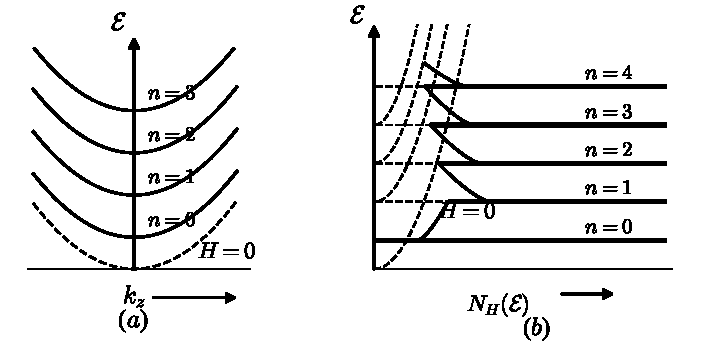
\includegraphics[width=0.72\textwidth]{fig_172.pdf}
\caption*{图 172\quad (a) 抛物线能带的磁量子化图式。(b) 态密度。}
\end{figure}

分配给每条抛物线各段的状态数由式 (9.67) 给出。对磁量子数 $n$ 的每个取值，我们都有一个简单的一维态密度问题。把能量 $\mathcal{E}$ 以下所有抛物线的贡献加起来，便得到总态密度函数
\begin{equation*}
\mathcal{N}_{H}(\mathcal{E})=\frac{1}{4\pi^{2}}\left(\frac{2m^{*}}{\hbar^{2}}\right)^{3/2}\hbar\omega_{H}\sum_{n}\left\{\mathcal{E}-\left(n+\frac{1}{2}\right)\hbar\omega_{H}\right\}^{-1/2}.
\tag{9.94}
\end{equation*}

\begin{figure}[H]
\centering
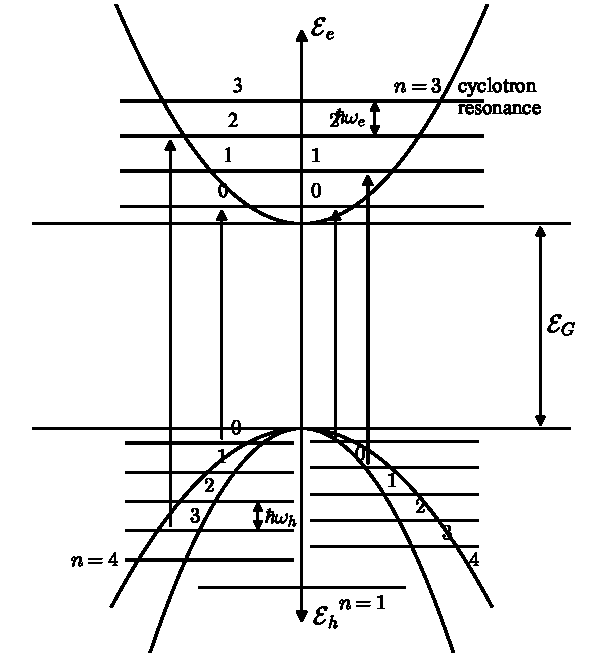
\includegraphics[width=0.72\textwidth]{fig_173.pdf}
\caption*{图 173\quad 半导体中具有两条空穴能带时的磁光跃迁。}
\end{figure}

当 $\omega_{H}\to 0$ 时，这个公式正确地积分后正确地回到标准的抛物线态密度函数 (4.33)。但磁场会在每个 Landau 能级处产生 $\mathcal{E}^{-1/2}$ 型的强 van Hove 奇异性（§2.5），这与 §9.7 中关于 de Haas--van Alphen 效应的一般论证相一致。

这类能级之间的跃迁将遵从选择定则 $\Delta n=\pm 1$；这不过是回旋共振（§9.2）的另一种描述方式。但态密度中的磁结构也足够宽，足以在其他能带的红外跃迁谱中被观察到，正如 §8.5 中所讨论的。这就是基本的磁光效应（magneto-optical effect）。

要解释实际的观测结果，还必须计及价带态的量子化，其 $\omega_{H}$ 和 $m^{*}$ 取不同的值（图 173）。对于一个在没有磁场时本来会发生的典型强跃迁，我们可以取矩阵元 (8.40) 与 $H$ 无关，并施加磁选择定则 $\Delta n=0$。于是联合态密度 (8.73) 便取与式 (9.94) 相同的形式；当 $\omega$ 与带间共振频率
\begin{equation*}
\hbar\omega_{n}=\mathcal{E}_{G}+\left(n+\frac{1}{2}\right)\hbar\left(\omega_{e}+\omega_{h}\right)
\tag{9.95}
\end{equation*}
相重合时，就会出现 $(\omega-\omega_{n})^{-1/2}$ 型的奇异性。不过在实际中，这些奇异性会因碰撞而展宽。

这样，这一现象就为测绘电子与空穴的回旋频率 $\omega_{e}$ 和 $\omega_{h}$ 提供了非常精确的手段，其能量范围覆盖带隙两侧。在一般的各向异性情形下，若同时存在价带简并以及能量对 $|\mathbf{k}|$ 的非抛物线型依赖，磁光谱可能非常复杂，但它提供了关于晶体电子能带结构的极为有价值的证据。

\section{磁击穿}

在本章中，我们讨论的一直是强磁场中的电子。特别地，我们研究了电子在被散射之前已回旋许多圈时出现的种种现象。我们已经看到，这时采用一种新的量子化图式是合宜的：在这一图式中，磁能级把 Bloch 图式中分立的各个允许态都吸收了进来。当然，如果存在散射，磁能级本身也会展宽，但只要 $\omega_{H}\tau\gg 1$，这一效应就可以忽略。

但是，我们提出的这种对每条轨道都满足式 (9.70) 的量子化图式，并不是在真正极其巨大的磁场中应当使用的终极图式。§9.6 中所用的准经典理论依赖于 §6.4 的等效哈密顿量原理；\emph{只有当我们能够忽略带间跃迁时，它才是有效的。}如果磁场非常大，这类跃迁就必然会发生——如果你愿意这么说，是通过隧穿发生的，正如 Zener 效应（§6.8）中那样——于是 \emph{Onsager} 图式 (9.70) 就会失效。

要理解这一效应，最容易的办法是从磁场极高的一端出发：在那里，电子波函数本质上就是带电粒子在磁场中自由运动的波函数，而晶格的晶体势仅作为微扰。把我们限制在垂直于磁场的二维空间内，我们在 $(k_{x},k_{y})$ 平面上便有一条圆形轨道。

现在引入如下形式的微扰
\begin{equation*}
\mathcal{V}(x)=\sum_{g}\mathcal{V}_{g}e^{igx}
\tag{9.96}
\end{equation*}
——即一系列相距 $2\pi/g$ 的平面。当轨道穿过区边界时，也就是说，当它沿 $x$ 方向的有效波矢 $k_{x}$ 等于 $\pm\frac{1}{2}g$ 时，就有可能发生 Bragg 衍射。轨道不再（比如说）沿 $AB$ 继续前进，而可能转到 $AC$ 方向，如此等等。

\begin{figure}[H]
\centering
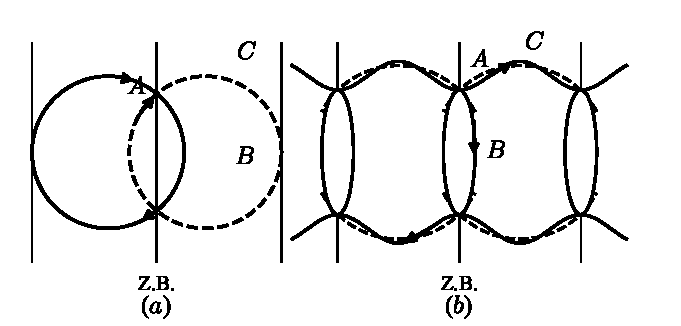
\includegraphics[width=0.72\textwidth]{fig_174.pdf}
\caption*{图 174\quad (a) 磁场中的自由电子轨道。(b) 在晶格的周期势中，轨道在区边界处被重新连接；但在强磁场下，轨道可能跳回自由电子的路径。}
\end{figure}

如果我们增大微扰的强度，那么 $A$ 处的轨道将在能量上分裂开，而 $AC$ 这条路径将成为优先的。此时电子便在通常的重复区图式中沿一条寻常的（开）轨道运动。图 174(a) 中圆的 $B$ 部分这时已被连接成费米面的一个单独分支，被完全分开地走完。

如果我们这时增大磁场，我们将回到圆形轨道图式。电子不再总是沿 $AC$ 前进，而是可能击穿能隙，或者说“隧穿”通过倒格子空间中分隔两条轨道的区域，发觉自己绕着 $B$ 运动了。

事实上，我们可以用 Zener 击穿的公式 (6.65) 来估计这个跃迁概率。电场 $E$ 能够引起穿过能隙 $\mathcal{E}_{\mathrm{gap}}$ 的隧穿，如果
\begin{equation*}
\frac{eEa\mathcal{E}^{0}}{(\mathcal{E}_{\mathrm{gap}})^{2}}>1,
\tag{9.97}
\end{equation*}
其中 $\mathcal{E}^{0}$ 是电子在能隙处的动能——实际上就是费米能 $\mathcal{E}_{F}$——而 $a$ 是相应的晶格间距。

现在，在重复区图式中趋向 $A$ 的电子具有速度
\begin{equation*}
v\sim\frac{\hbar k_{F}}{m},
\tag{9.98}
\end{equation*}
其中 $k_{F}$ 是费米半径。这在区边界处并不严格成立，因为等能面会因能隙的存在而发生畸变，但我们正假设这个畸变很小。

电子以这一速度横越磁场运动，会产生一个 Lorentz 力，它等同于一个强度为
\begin{equation*}
E\sim\frac{vH}{c}
\tag{9.99}
\end{equation*}
、方向与 $v$ 成直角的电场。如果式 (9.97) 得到满足，也就是说，如果参数
\begin{equation*}
\frac{ev\mathbf{H}}{c}\,\frac{a\mathcal{E}^{0}}{(\mathcal{E}_{\mathrm{gap}})^{2}}\approx\frac{e\hbar}{mc}\,H\,\frac{k_{F}a\mathcal{E}_{F}}{(\mathcal{E}_{\mathrm{gap}})^{2}}
\tag{9.100}
\end{equation*}
大于 1，这个场就能引起隧穿。由 (3.3)，乘积 $k_{F}a$ 是一个量级为 1 的数。利用 (9.4)，磁击穿（magnetic breakdown）的条件便成为
\begin{equation*}
\frac{\hbar\omega_{H}\mathcal{E}_{F}}{(\mathcal{E}_{\mathrm{gap}})^{2}}>1.
\tag{9.101}
\end{equation*}

这个条件远不如（我们不妨这么说）磁轨道的间隔必须大于能隙这样的条件那样苛刻。对某些金属，在 100 kG 量级的磁场中它就变得重要起来，并且会在 de Haas--van Alphen 效应以及其他现象中引起各种不同面积的新轨道的出现。

 % 本文件由 scripts/assemble.py 自动装配，勿手改（改 parts/ 后重跑）
% 第10章 磁性

\chapter{磁性}

\epigraphbook{万物皆始于秩序，故亦将终于秩序，并将依循秩序的制定者、\\天上之城的神妙数学，再度开始。}{SIR THOMAS BROWNE}

\section{轨道磁化率}

在本章中，我们所关注的是固体的磁化率本身，而不涉及磁场对固体其他性质（例如电导率）的影响。这是一个很大的课题，我们无法细致处理。例如，我们将略去大多数磁共振（magnetic resonance）现象。我们也不讨论技术上十分重要的、可永久磁化的材料的那些宏观性质的理论，例如磁滞（hysteresis）、矫顽力（coercivity）、剩磁（remanent magnetism）等等；这些性质本质上取决于样品被自发磁化而分成若干磁畴（domains），各磁畴的磁矩取向彼此不同。我们甚至不打算考虑划分磁化不同的磁畴的 Bloch 壁（Bloch wall）的优美理论——这种壁在施加磁场时还可以被驱使移动。

我们首先考虑\emph{非磁性固体}，在其中完全不必怀疑原子或离子携带有局域磁矩。我们也忽略电子自旋，或者假定所有自旋都紧紧地配对。即便如此，电子的轨道运动仍会对磁化率有贡献。

最简单的情形是每个原子或离子都由电子的闭合壳层组成，且激发到更高状态的能量很大。众所周知，这就导致抗磁性（diamagnetism）；磁化率为负，近似地由下式给出：
\begin{equation*}
\chi=-\frac{Ze^{2}N}{6mc^{2}}\,\overline{r^{2}},
\tag{10.1}
\end{equation*}
其中 $Z$ 是原子中电子的总数，$N$ 是单位体积中的原子数，$\overline{r^{2}}$ 是每个原子周围电子电荷云的方均半径。这正是我们处理稀有气体固体、或者离子晶体中离子的贡献时应当使用的那类公式。

上述结果本质上来自一阶微扰能量
\begin{equation*}
\left\langle 0\,\left|\frac{e^{2}}{2mc^{2}}A^{2}\right|\,0\right\rangle,
\tag{10.2}
\end{equation*}
其中 $\mathbf{A}$ 是磁场的矢量势，$|0\rangle$ 是每个原子的基态。当我们按照磁场中哈密顿量的标准表达式，把动能写成
\begin{equation*}
T=\frac{1}{2m}\left(\frac{\hbar}{i}\nabla-\frac{e}{c}\mathbf{A}\right)^{2}
\tag{10.3}
\end{equation*}
的形式时（如式 (9.51) 那样），上式便自动出现。

但是，如果原子存在激发态，比如说 $|n\rangle$，其轨道矩不为零，那么 (10.3) 中线性于 $\mathbf{A}$ 的项——也就是给出算符
\begin{equation*}
\frac{e}{2mc}\,\mathbf{H}\cdot\mathbf{L}=\mathbf{H}\cdot\boldsymbol{\mu}_{L},
\tag{10.4}
\end{equation*}
的那一项——就可能把这些激发态混入基态，其中 $\mathbf{L}$ 是电子的轨道角动量算符，而 $\boldsymbol{\mu}_{L}$ 是与之成比例的通常的磁矩算符。在二阶微扰中，这一项对能量的贡献为
\begin{equation*}
\delta\mathcal{E}=\sum_{n}\frac{|\langle 0|\mathbf{H}\cdot\boldsymbol{\mu}_{L}|n\rangle|^{2}}{\mathcal{E}_{0}-\mathcal{E}_{n}}
\tag{10.5}
\end{equation*}
它是正的，并且是 $H$ 的二次式。这就是原子、离子或分子的恒定的 van Vleck 顺磁性（van Vleck paramagnetism）的来源。

实践表明，把 (10.2) 和 (10.5) 应用于实际固体极其复杂；这就是我们只在原则上引用这些公式的原因。但我们从 (10.5) 中注意到，当激发能量变小时——例如在填满的能带之上有小的带隙时——这一贡献应当增大。当这个带隙趋于零，也就是当我们拥有自由载流子时，会发生什么呢？

这时理论又变得非常复杂，但对自由电子却存在精确解。在 §9.6 中我们导出了磁场中自由电子的能级；只要贯彻那套导致 de Haas--van Alphen 效应的 §9.7 的形式框架，算出整个电子气能量的平均变化并不困难。我们不寻求自由能中的振荡项，而是集中于那些作为 $H$ 的单调函数的项。例如，在 (9.80) 中我们略去了
\begin{equation*}
\frac{1}{4\pi^{2}s^{2}kT}\left[f^{0}(\mathcal{E})\frac{\partial\mathcal{E}}{\partial x}\right]_{x=0}
=\frac{1}{4\pi^{2}s^{2}kT}\,\frac{e\hbar H}{mc}\left[f^{0}(\mathcal{E})\right]_{x=0}
\tag{10.6}
\end{equation*}
（其中利用了 (9.82) 和 (9.58)）。

但这是 (9.79) 中的一项，而 (9.79) 中含有对所有 $s$ 值的求和以及对 Fermi 球的所有切片 $k_{z}$ 的积分。于是，对自由能的总贡献（除去 (9.79) 中与 $H$ 无关的前两项）便是
\begin{align*}
\Delta F_{L} &=-2kT\sum_{s=1}^{\infty}(-1)^{s}\int_{-\infty}^{\infty}\frac{eH}{2\pi^{2}\hbar c}\,\frac{1}{4\pi^{2}s^{2}kT}\,\frac{e\hbar H}{mc}\left[f^{0}(\mathcal{E})\right]_{x=0}dk_{z}\\
&=-\frac{1}{4\pi^{4}}\left(\frac{eH}{c}\right)^{2}\frac{1}{m}\int_{-\infty}^{\infty}\left[f^{0}(\mathcal{E})\right]_{x=0}dk_{z}\sum_{s=1}^{\infty}\frac{(-1)^{s}}{s^{2}}.
\tag{10.7}
\end{align*}
对 $k_{z}$ 的积分本质上量度的是 k 空间中沿 Fermi 球轴线的填充区域的长度，而对 $s$ 的求和给出 $-\frac{1}{12}\pi^{2}$。把它表示成磁化率，我们便得到 \emph{Landau 抗磁性}（Landau diamagnetism）
\begin{equation*}
\chi_{L}=-\frac{e^{2}k_{F}}{12\pi^{2}mc^{2}}.
\tag{10.8}
\end{equation*}

这个结果为负，是因为能级的聚束倾向于增大系统的总能量。从图 171 可以看到这一点。只有当 费米能级恰好位于两个量子化能级的正中间时，电子才能够“凝聚”到各自相应的管道上而不改变其平均能量。当一个量子化能级逼近 费米能级时，它会把电子一同带上去；这就是 $\Delta F_{L}$ 为正的原因。磁化率与温度无关，因为这是一种平均效应，并不要求能级间隔 $\hbar\omega_{H}$ 大于 $kT$。

按照 §9.7 论证的思路，对任意 费米面这一更一般的情形来计算 (10.7) 并不困难。但这样得到的结果并不正确。周期晶格中电子的 Landau 抗磁性需要更复杂的分析，我们在此不拟给出。此外，在 van Vleck 贡献与 Landau 贡献之间还存在交叉项。

\section{自旋顺磁性}

共享同一轨道态的、自旋相反的电子之间的简并，会被磁场解除。在金属中，这引起电子在两种自旋取向之间重新分布，从而产生一个磁矩。这个效应的计算是初等的。假设我们区分 + 自旋与 $-$ 自旋的电子（相对于 $\mathbf{H}$ 的方向）。那么它们的能量将为
\begin{equation*}
\left.\begin{aligned}
\mathcal{E}_{\mathbf{k}+} &= \mathcal{E}(\mathbf{k})-\mu_{0}H,\\
\mathcal{E}_{\mathbf{k}-} &= \mathcal{E}(\mathbf{k})+\mu_{0}H,
\end{aligned}\right\}
\tag{10.9}
\end{equation*}
其中 $\mathcal{E}(\mathbf{k})$ 是不存在磁场时的能量，而 $\mu_{0}$ 是电子的磁矩。

每个状态中的电子数将由两个不同的 Fermi--Dirac 分布给出，如同式 (4.8) 那样，但具有相同的化学势 $\zeta$。于是，正如我们在图 175 中看到的，+ 自旋态容纳的电子比先前要多——总数为
\begin{equation*}
n_{+}=\int_{0}^{\infty}\frac{1}{2}\,\mathcal{N}(\mathcal{E})\,f^{0}(\mathcal{E}_{\mathbf{k}+})\,d\mathcal{E},
\tag{10.10}
\end{equation*}
这是因为在原来能量 $\mathcal{E}$ 处的态密度，是在 + 自旋与 $-$ 自旋的电子之间平分的。

\begin{figure}[H]
\centering
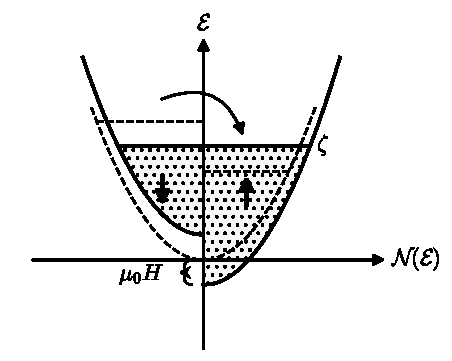
\includegraphics[width=0.72\textwidth]{fig_175.pdf}
\caption*{图 175\quad 磁场中“上”自旋与“下”自旋的 费米分布。}
\end{figure}

对于负自旋电子的密度有相应的公式。两者之差给出一个磁矩
\begin{align*}
M &=\mu_{0}(n_{+}-n_{-})\\
&=\mu_{0}\int_{0}^{\infty}\tfrac{1}{2}\{f_{0}(\mathcal{E}-\mu_{0}H)-f_{0}(\mathcal{E}+\mu_{0}H)\}\,\mathcal{N}(\mathcal{E})\,d\mathcal{E}\\
&\approx\mu_{0}^{2}H\int_{0}^{\infty}\left(-\frac{\partial f^{0}}{\partial\mathcal{E}}\right)\mathcal{N}(\mathcal{E})\,d\mathcal{E}\\
&=\mu_{0}^{2}H\,\mathcal{N}(\mathcal{E}_{F})
\tag{10.11}
\end{align*}
由式 (4.18)。

这个正的磁矩导致 Pauli 顺磁性（Pauli paramagnetism）。它不依赖于温度，并且直接量度 费米能级处的态密度。因此，原则上它应当与电子比热（§4.7）直接相关联；不过，当人们对多电子相互作用作出修正之后（§5.8），这种严格的等价性便不复存在。在实践中做这类比较的困难在于，抗磁性修正 (10.8) 并非可以忽略，而人们对它又知道得不够准确。不过在有些情形下，可以通过观察传导电子的电子自旋共振，直接测量自旋磁化率。

对自由电子气，容易证明
\begin{align*}
\chi_{P} &=\mu_{0}^{2}\,\mathcal{N}(\mathcal{E}_{F})\\
&=\frac{e^{2}k_{F}}{4\pi^{2}mc^{2}},
\tag{10.12}
\end{align*}
它恰好是 Landau 项 (10.8) 数值的三倍。但是，晶格对这两类磁化率的影响却截然不同。例如，假设 费米面是球形的，但“有效质量”变为 $m^{*}$。容易证明，$\chi_{P}$ 依赖于态密度，因而正比于 $m^{*}$；而 $\chi_{L}$ 由电子的轨道运动决定，不经过 Bohr 磁子的介入，所以将\emph{反比}于 $m^{*}$。

与自旋磁化率相联系的另一个现象是 Knight 移动（Knight shift）。在磁场 $\mathbf{H}$ 中，电子自旋被极化，每个电子具有平均磁矩
\begin{equation*}
\langle\boldsymbol{\mu}_{e}\rangle=\frac{1}{n}\,\chi_{P}\,\mathbf{H}.
\tag{10.13}
\end{equation*}
位于 $\mathbf{r}$ 处的一个电子，将与位于 $\mathbf{R}$ 处的原子核的磁矩 $\boldsymbol{\mu}_{I}$ 通过“接触相互作用”（contact interaction）
\begin{equation*}
\mathcal{H}_{\text{int.}}=\tfrac{8}{3}\pi\,(\boldsymbol{\mu}_{I}\cdot\boldsymbol{\mu}_{e})\,\delta(\mathbf{r}-\mathbf{R}),
\tag{10.14}
\end{equation*}
发生作用，这个效应在核共振理论中是众所周知的。把 (10.13) 代入 (10.14)，我们得到一个平均能量
\begin{align*}
\langle\mathcal{H}_{\text{int.}}\rangle &=\tfrac{8}{3}\pi\,\frac{\chi_{P}}{n}\,H\,|\psi(0)|^{2}\,\mu_{I}\\
&=\Delta\mu_{I}\cdot\mathbf{H},
\tag{10.15}
\end{align*}
姑且这样记，其中 $|\psi(0)|^{2}$ 是波函数在核处的模方。这个能量被解释为核的表观磁矩出现一个改变量 $\Delta\mu_{I}$——即它在磁场中共振频率的移动。

显然，Knight 移动应当正比于 $\chi_{P}$。但还有一个因子 $|\psi(0)|^{2}$，它无法由任何独立的实验给出。原则上这只涉及 费米面上的态，因此人们说它“量度了 费米能级处波函数中 $s$ 型成分的多少”。Knight 移动是一个容易测定的好物理量，但它的结果却不那么容易解释。

\section{居里--外斯定律与铁磁性}

现在我们假设每个原子的行为像一个小磁体，磁矩为 $\boldsymbol{\mu}$，例如可以来自过渡金属或稀土元素的离子中 $d$ 电子或 $f$ 电子的未满壳层。在磁场 $\mathbf{H}$ 中，每个小磁体将具有能量 $-\boldsymbol{\mu}\cdot\mathbf{H}$。假设每个原子都与近邻无关；由于它是局域的，它满足 Boltzmann 统计。磁矩为 $\boldsymbol{\mu}$ 的原子所占的比例将正比于
\begin{equation*}
n(\boldsymbol{\mu})=e^{\boldsymbol{\mu}\cdot\mathbf{H}/kT}.
\tag{10.16}
\end{equation*}

如果我们假设每个磁体都可以自由转动，那么平均磁矩必定是
\begin{equation*}
\langle\boldsymbol{\mu}\rangle=\int\boldsymbol{\mu}\,e^{\boldsymbol{\mu}\cdot\mathbf{H}/kT}d\Omega\,\Big/\int e^{\boldsymbol{\mu}\cdot\mathbf{H}/kT}d\Omega,
\tag{10.17}
\end{equation*}
其中 $d\Omega$ 是 $\boldsymbol{\mu}$ 转动时的立体角元。单位体积内 $N$ 个这种原子的集合将具有磁化率
\begin{align*}
\chi &=N\frac{\partial\langle\boldsymbol{\mu}\rangle}{\partial\mathbf{H}}=\int(N/kT)\,\boldsymbol{\mu}\boldsymbol{\mu}\,e^{\boldsymbol{\mu}\cdot\mathbf{H}/kT}d\Omega\,\Big/\int e^{\boldsymbol{\mu}\cdot\mathbf{H}/kT}d\Omega\\
&\approx\frac{N}{kT}\langle\boldsymbol{\mu}\boldsymbol{\mu}\rangle=\frac{1}{3}\,\frac{N\langle\mu^{2}\rangle}{kT}
\tag{10.18}
\end{align*}
此时 $H$ 已小到指数项可以忽略；并且我们已经把并矢张量 $\boldsymbol{\mu}\boldsymbol{\mu}$ 的平均，同矢量 $\boldsymbol{\mu}$ 之长度的平方 $\mu^{2}$ 的平均作了比较。

如今对我们来说，更自然的做法是把每个磁体同一个自旋角动量 $\mathbf{S}$ 联系起来，它沿磁场方向量子化：
\begin{equation*}
\boldsymbol{\mu}\cdot\mathbf{H}=\beta HS_{z},
\tag{10.19}
\end{equation*}
其中 $S_{z}$ 以整数台阶从 $S$ 变到 $-S$，而 $\beta$ 是 Bohr 磁子的两倍。例如，设 $S=\frac{1}{2}$。这时在 (10.17) 中我们遇到的是求和而不是积分：
\begin{align*}
\langle\boldsymbol{\mu}\rangle &=\beta S\left[\frac{e^{\beta SH/kT}-e^{-\beta SH/kT}}{e^{\beta SH/kT}+e^{-\beta SH/kT}}\right]\\
&=\beta S\,\tanh\frac{\beta SH}{kT}.
\tag{10.20}
\end{align*}

在 $H$ 很小的极限下，这个结果便与 (10.18) 相同，只要我们注意到，按照总角动量大小的规则，
\begin{equation*}
\langle\mu^{2}\rangle=S(S+1)\beta^{2}.
\tag{10.21}
\end{equation*}

结果 (10.18) 就是著名的顺磁磁化率的 \emph{Curie 定律}（Curie Law）。某些类型的固体近似地服从它，尤其是磁性原子或离子在晶体中彼此相距很远的那些固体，因为这时独立性假设成立。

然而在许多物质中，近邻自旋之间存在相互作用。为了近似地把这一点考虑进去，可以引入 \emph{Weiss 场}（Weiss field）
\begin{equation*}
\mathbf{H}_{I}=\lambda N\langle\boldsymbol{\mu}\rangle.
\tag{10.22}
\end{equation*}
这个场被认为来自每个原子所处的磁化平均环境——不过，用来量度相互作用强度的参量 $\lambda$，我们让它保持任意。

作用在一个原子上的总场现在是 $\mathbf{H}+\mathbf{H}_{I}$。把它代替 $\mathbf{H}$ 代入 (10.20)，我们近似地得到
\begin{equation*}
N\langle\boldsymbol{\mu}\rangle=\frac{1}{3}\,\frac{N\langle\mu^{2}\rangle}{kT}\left(\mathbf{H}+\lambda N\langle\boldsymbol{\mu}\rangle\right),
\tag{10.23}
\end{equation*}
由此得
\begin{align*}
\chi &\equiv N\left\langle\frac{\partial\boldsymbol{\mu}}{\partial\mathbf{H}}\right\rangle\\
&=\frac{N\langle\mu^{2}\rangle}{3k(T-\theta)},
\tag{10.24}
\end{align*}
其中
\begin{equation*}
\theta=\frac{\lambda N\langle\mu^{2}\rangle}{3k}.
\tag{10.25}
\end{equation*}
这就是所谓的\emph{居里--外斯定律}（Curie--Weiss law），它描述许多固体的磁化率行为。

参量 $\theta$ 显然具有温度的量纲。如果在 (10.24) 中 $T<\theta$ 会怎么样？磁化率似乎会先变为无穷大，然后变为负值。我们必须回到 (10.20)，求解方程
\begin{equation*}
N\langle\boldsymbol{\mu}\rangle=N\beta S\,\tanh\left\{\frac{\beta S}{kT}\left(\lambda N\langle\boldsymbol{\mu}\rangle+H\right)\right\}.
\tag{10.26}
\end{equation*}
当 $H=0$ 时，通常的解是 $\langle\boldsymbol{\mu}\rangle=0$；但当 $T<\theta$ 时，我们发现还有另一个 $\langle\boldsymbol{\mu}\rangle\neq 0$ 的根。这个根很容易用图解法定位；在温度 $T=0$ 时它显然趋于
\begin{equation*}
\mathbf{M}(0)=N\beta S.
\tag{10.27}
\end{equation*}

\begin{figure}[H]
\centering
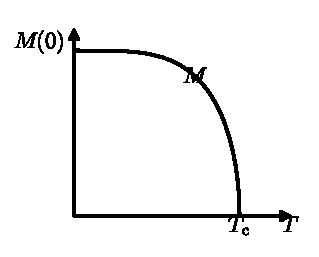
\includegraphics[width=0.72\textwidth]{fig_176.pdf}
\caption*{图 176\quad 铁磁体中的自发磁化。}
\end{figure}

这时系统的行为就好像每一个磁矩都平行排列一样；我们说这固体是\emph{铁磁性的}（ferromagnetic），并且看到，即使在不存在磁场时它也表现出很大的自发磁化。当我们使晶体升温时，自发磁化不断减小，直到在一个完全确定的温度——\emph{居里温度}（Curie temperature）——处消失：
\begin{equation*}
T_{\mathrm{C}}=\theta.
\tag{10.28}
\end{equation*}

\section{交换相互作用}

用居里温度 (10.25) 来衡量，Weiss 内场非常之大——远大于一个磁体阵列的普通内禀偶极场。在许多铁磁物质中，系数 $\lambda$ 并非 $\frac{4}{3}\pi$（对 Lorentz 场 (8.52) 而言它本可以取这个值），而是 1000 的量级。

通常把这个表观场归因于相邻原子上电子自旋之间的\emph{交换相互作用}（exchange interaction）。对于 Heisenberg 和 Dirac 的严格局域模型，我们可以给第 $\boldsymbol{l}$ 个格点上的原子指派一个总自旋算符 $\boldsymbol{\mathsf{S}}_{\boldsymbol{l}}$，并写下哈密顿量
\begin{equation*}
\mathcal{H}=-\sum_{\boldsymbol{l}\boldsymbol{l}'}J_{\boldsymbol{l}\boldsymbol{l}'}\,\boldsymbol{\mathsf{S}}_{\boldsymbol{l}}\cdot\boldsymbol{\mathsf{S}}_{\boldsymbol{l}'}-\beta\mathbf{H}\cdot\sum_{\boldsymbol{l}}\boldsymbol{\mathsf{S}}_{\boldsymbol{l}}.
\tag{10.29}
\end{equation*}
\emph{交换积分}（exchange integral）$J_{\boldsymbol{l}\boldsymbol{l}'}$ 是格点 $\boldsymbol{l}$ 与 $\boldsymbol{l}'$ 相对位置的函数，但只有当 $\boldsymbol{l}-\boldsymbol{l}'$ 为一两个格点间距时它才比较大。

我们可以把这个哈密顿量写成
\begin{equation*}
\mathcal{H}=-\sum_{\boldsymbol{l}}\bigl\{\sum_{\boldsymbol{l}'}J_{\boldsymbol{l}\boldsymbol{l}'}\boldsymbol{\mathsf{S}}_{\boldsymbol{l}'}+\beta\mathbf{H}\bigr\}\cdot\boldsymbol{\mathsf{S}}_{\boldsymbol{l}}.
\tag{10.30}
\end{equation*}
试想温度极低时会出现什么情形：那时所有自旋都排列整齐，以致对一切 $\boldsymbol{l}'$ 有
\begin{equation*}
\langle\beta\boldsymbol{\mathsf{S}}_{\boldsymbol{l}'}\rangle\approx\langle\boldsymbol{\mu}\rangle,
\tag{10.31}
\end{equation*}
于是我们可以把 (10.30) 中的第一项辨认成内场
\begin{align*}
\beta\mathbf{H}_{I}&=\sum_{\boldsymbol{l}'}J_{\boldsymbol{l}\boldsymbol{l}'}\boldsymbol{\mathsf{S}}_{\boldsymbol{l}'}\\
&=\frac{1}{\beta}\Bigl(\sum_{\boldsymbol{l}'}J_{\boldsymbol{l}\boldsymbol{l}'}\Bigr)\langle\boldsymbol{\mu}\rangle,
\tag{10.32}
\end{align*}
即
\begin{equation*}
\lambda=\frac{1}{N\beta^{2}}\Bigl(\sum_{\boldsymbol{l}'}J_{\boldsymbol{l}\boldsymbol{l}'}\Bigr)
\tag{10.33}
\end{equation*}
或者，用居里温度 (10.25) 来表示，
\begin{equation*}
k\theta=\frac{1}{3}S(S+1)\sum_{\boldsymbol{l}'}J_{\boldsymbol{l}\boldsymbol{l}'}.
\tag{10.34}
\end{equation*}
这便用系统转变为铁磁态所处的温度给出了交换相互作用的大小。

这个\emph{自旋哈密顿量}（spin Hamiltonian）(10.29) 的性质将是本章其余部分的主要论题。但是，它作为一个基本假设是否有充分的根据呢？对这个问题已有过许多不同的回答，而它正是铁磁性作为一种物理现象之谜的核心所在。

从群论的论证容易证明：相互作用取自旋算符的标量积这一形式，至少是最简单的可能形式，尽管还可能存在更复杂的其他项，例如\emph{偶极–偶极相互作用}（dipole–dipole interaction），
\begin{equation*}
\mathcal{H}_{\mathrm{dip.-dip.}}=\beta^{2}\biggl\{\frac{\boldsymbol{\mathsf{S}}_{1}\cdot\boldsymbol{\mathsf{S}}_{2}}{R^{3}}-\frac{3(\boldsymbol{\mathsf{S}}_{1}\cdot\mathbf{R})(\boldsymbol{\mathsf{S}}_{2}\cdot\mathbf{R})}{R^{5}}\biggr\},
\tag{10.35}
\end{equation*}
其中两个自旋相距 $\mathbf{R}$（一个矢量）。

同样众所周知的是，同一原子上或相邻原子上的电子自旋倾向于通过交换效应耦合起来——这是 Pauli 原理的一个推论。例如，若 $\phi_{a}$ 和 $\phi_{b}$ 是我们“放入两个电子”的两个波函数，那么按照这两个电子的自旋是平行还是反平行，我们可以构造出两类状态。这些状态就是对称与反对称组合
\begin{align*}
\Phi_{S}(\mathbf{r}_{1},\mathbf{r}_{2})&=2^{-\frac{1}{2}}\bigl\{\phi_{a}(\mathbf{r}_{1})\phi_{b}(\mathbf{r}_{2})+\phi_{a}(\mathbf{r}_{2})\phi_{b}(\mathbf{r}_{1})\bigr\},\\
\Phi_{A}(\mathbf{r}_{1},\mathbf{r}_{2})&=2^{-\frac{1}{2}}\bigl\{\phi_{a}(\mathbf{r}_{1})\phi_{b}(\mathbf{r}_{2})-\phi_{a}(\mathbf{r}_{2})\phi_{b}(\mathbf{r}_{1})\bigr\},
\tag{10.36}
\end{align*}
其中 $\Phi_{S}$ 属于反平行自旋（\emph{单态}，singlet state），而 $\Phi_{A}$ 属于平行自旋（\emph{三重态}，triplet state）。现在，如果我们计算库仑能 $e^{2}/|\mathbf{r}_{1}-\mathbf{r}_{2}|$ 在这两个态中的平均值，就会发现二者相差一个量
\begin{equation*}
2\iint\phi_{a}^{*}(\mathbf{r}_{1})\phi_{b}^{*}(\mathbf{r}_{2})\frac{e^{2}}{|\mathbf{r}_{1}-\mathbf{r}_{2}|}\phi_{a}(\mathbf{r}_{2})\phi_{b}(\mathbf{r}_{1})\,\mathrm{d}\mathbf{r}_{1}\,\mathrm{d}\mathbf{r}_{2},
\tag{10.37}
\end{equation*}
这就是交换积分。容易把这个差改写成如下形式，使它表示 $2J\,\boldsymbol{\mathsf{S}}_{1}\cdot\boldsymbol{\mathsf{S}}_{2}$ 在 $\boldsymbol{\mathsf{S}}_{1}$ 与 $\boldsymbol{\mathsf{S}}_{2}$ 平行和反平行两种情形下取值之差。于是，$J$ 的正负与大小便取决于这个积分的正负与大小。

有两种众所周知的情形。设两个电子属于同一原子，但并未填满一个闭合壳层。这时，库仑相互作用与原子轨道 $\phi_{a}$、$\phi_{b}$ 的形式使得 $J$ 为正；电子自旋倾向于排列起来，在与壳层中待填充的独立态数目相容的前提下使总自旋最大。这就是 Hund 规则（Hund's rule），它解释了为什么过渡金属离子的未满 d 壳层中的电子倾向于组合起来，赋予离子一个很大的永久磁矩（§5.5）。研究这类离子处于复杂晶体中各种环境时的顺磁性与磁共振性质，是物理学的一个重要分支。

但我们在这里关心的是不同离子上的电子自旋之间的相互作用——结果发现，在这种情形下算出的 $J$ 几乎总是负的，即倾向于使相邻格点上的自旋反平行。这方面最简单的例子是氢分子的 Heitler–London 模型，其中成键态的电子自旋是配对的。在 §4.2 中处理共价键时，我们曾把这一点视为理所当然。

因此，在这个基础上很难解释许多金属——通常是“过渡”族元素——具有铁磁性这一事实。我们可以理解为什么每个离子中的 d 电子倾向于组合成一个总自旋——在 Fe 中大到 $\frac{5}{2}$；却无法理解为什么相邻离子上的磁矩之间的相互作用会有利于平行取向。问题还因如下事实（§4.1）而更加复杂：这些所谓的 d 电子并非严格局域在特定的离子上，而是处于从原子到原子相互交叠、形成窄能带的状态。这个窄带又与普通的 s 带杂化，在 s 带中电子可以十分自由地传导。Heisenberg 模型哈密顿量 (10.29) 尽管作为金属铁磁性的唯象理论颇为成功，却需要从第一性原理出发加以认真的重新考察。这个微妙问题——固体理论中最重要的基本问题之一——的若干方面将在 §10.5–§10.6 中讨论。

\section{能带铁磁性}

从 Heisenberg 模型的局域自旋转向相反的极端，让我们把所有磁性电子都放进一个由 Bloch 态构成的能带。令 $n_{\mathbf{k}+}$ 为具有 + 自旋的态 $|\mathbf{k}\rangle$ 的占据数。在 Stoner 的\emph{集体电子模型}（collective electron model）中，我们在电子哈密顿量上添加如下一项：
\begin{equation*}
\mathcal{H}_{\mathrm{int.}}=\frac{U}{N}\sum_{\mathbf{k},\mathbf{k}'}n_{\mathbf{k}+}n_{\mathbf{k}'-}.
\tag{10.38}
\end{equation*}
于是，每一对自旋相反的电子都贡献一个大小为 $U/N$ 的正的“交换”能，它或许来自这两个电子偶尔同时栖身于同一原子的 d 壳层，但不一定恰好由像 (10.37) 那样的积分严格表示。自旋相同的电子的贡献则无须显式计入，因为它们可以归并到能量零点的定义之中。

虽然这一项可以解释为给出一个像 (10.22) 那样的内场，但我们现在处理的是 费米–狄拉克 分布，可以沿用 §10.2 的论证。令 $n_{\sigma}$ 为每原子中自旋为 $\sigma$ 的电子总数。代替 (10.9)，一个 + 自旋电子的能量为
\begin{equation*}
\mathcal{E}_{\mathbf{k}+}=\mathcal{E}(\mathbf{k})-\mu_{0}H+Un_{-},
\tag{10.39}
\end{equation*}
对 $-$ 自旋的电子有类似的式子。

两个电子集合的化学势仍然相同，因此我们必须满足如下方程：
\begin{equation*}
n\langle\mu\rangle=\mu_{0}\int_{0}^{\infty}\frac{1}{2}\bigl\{f^{0}(\mathcal{E}_{\mathbf{k}+})-f^{0}(\mathcal{E}_{\mathbf{k}-})\bigr\}\mathcal{N}(\mathcal{E})\,d\mathcal{E},
\tag{10.40}
\end{equation*}
以及
\begin{equation*}
n=\int\frac{1}{2}\bigl\{f^{0}(\mathcal{E}_{\mathbf{k}+})+f^{0}(\mathcal{E}_{\mathbf{k}-})\bigr\}\mathcal{N}(\mathcal{E})\,d\mathcal{E}.
\tag{10.41}
\end{equation*}
在 $H\to 0$、$T\to 0$ 的极限下，这些方程有一个与 (10.11) 类似的解。磁化率取如下形式：
\begin{equation*}
\chi=\frac{\mu_{0}^{2}\mathcal{N}(\mathcal{E}_{F})}{1-\frac{1}{2}U\mathcal{N}(\mathcal{E}_{F})}
\tag{10.42}
\end{equation*}
就好像我们只是把 Pauli 磁化率 (10.12) 增大了一个因子 $1/\{1-\frac{1}{2}U\mathcal{N}(\mathcal{E}_{F})\}$。交换相互作用 (10.38) 由于偏向平行自旋，使系统更容易被极化。

\begin{figure}[H]
\centering
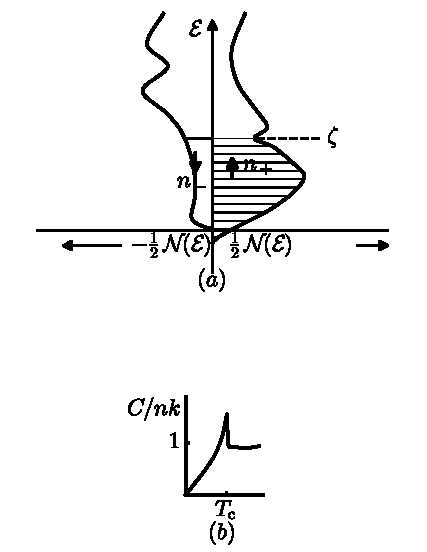
\includegraphics[width=0.72\textwidth]{fig_177.pdf}
\caption*{图 177\quad (a) 能带铁磁性；(b) 铁磁金属的电子比热。}
\end{figure}

但是，当交换场强到足以使
\begin{equation*}
\frac{1}{2}U\mathcal{N}(\mathcal{E}_{F})>1,
\tag{10.43}
\end{equation*}
时，这个形式解显然是不稳定的。这标志着向铁磁性的转变。为使 (10.39)–(10.41) 相互一致，我们必须让 $n_{+}$（比如说）远大于 $n_{-}$，从而使系统具有一个永久磁矩。随后便可数值求解这些方程，给出 $\langle\mu\rangle$ 作为温度的函数。其结果在定性上与 (10.26) 的结果并无明显不同。系统表现出一个居里温度，在居里温度以下磁矩饱和到近乎恒定的值；在居里点以上，理论也预言了某种类似于居里–外斯定律 (10.24) 的行为。

在这个模型中，不难显式计算出与这一转变相联系的比热。能量（参见 §4.7）可以作为 $T$ 的函数算出，再对它求导便给出比热。结果表明，$C_{\mathrm{el.}}$ 在居里
点处出现不连续，紧挨其下方是一个尖锐的峰。这又是向铁磁性转变时观测到的一个特征，尽管理论并不能在所有细节上都重现该峰的确切形状。

铁磁性的巡游电子（itinerant electron）图像对铁磁金属绝大多数观测性质的解释，与局域自旋模型同样成功。它也与普遍的能带理论（§3.10）、输运理论以及费米面研究相一致；例如，在其中可以观察到两套分立的能带系统，分别容纳“向上”自旋与“向下”自旋的电子。另一方面，“交换”能 $U$ 的确切本性一点也不清楚，而且有独立的证据表明磁矩存在某种程度的表观局域化（§10.6、§10.11）。当前最好的看法是：对具有 d 带的过渡金属倾向于能带模型，而稀土金属中部分填充的 f 态里的自旋，则似乎总是表现得如同按 Heisenberg 方式局域化。

如 §8.3 所述，有些物质是铁电体（ferro-electric）：它们在没有电场的情况下也能携带永久电矩。这一现象在宏观上与铁磁性相似，但其来源是一个复杂得多、也极不寻常的微观效应。它出自某些晶体结构的一种能力：使自己发生轻微畸变，从而让晶格的每一个晶胞都带有一个偶极矩。

\section{磁性杂质}

过渡元素或稀土元素的原子溶入普通金属后，往往保留局域磁矩。这是一系列有趣的实验现象和理论概念的源泉。用相移语言（§5.5）所作的 Friedel 解释，与通过 Anderson 哈密顿量（Anderson Hamiltonian）的传统描述互为补充；借助后者，可以用少数几个唯象参量对这类现象的许多特征作出半定量估计。

首先我们假设：自旋相反的电子之间的“交换”或“关联”排斥，只有当二者处在同一个能量为 $\mathcal{E}_d$ 的原子 $d$ 能级上时才起作用。利用式 (10.38) 中已经用过的简化 Hartree--Fock 近似，我们写出

\begin{equation*}
\mathcal{H}_{dd} = U n_{d+} n_{d-} \tag{10.44}
\end{equation*}
其中 $n_{d\sigma}$ 表示自旋为 $\sigma$ 的 $d$ 电子的平均数目。倘若过渡元素溶入普通金属后这些原子能级仍保持完全锐利，它们无疑会被极化——比方说 $n_{d+}$ 取尽可能大的值，而 $n_{d-}$ 取尽可能小的值——这正是 §10.5 所讨论的那类情形的一个夸张版本。在这种组态下，各能级的有效能量被劈开，即（图 178）

\begin{equation*}
\mathcal{E}_{d\sigma} = \mathcal{E}_d + U n_{d\sigma}. \tag{10.45}
\end{equation*}
\begin{figure}[H]
\centering
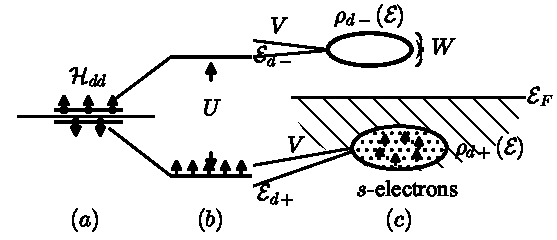
\includegraphics[width=0.72\textwidth]{fig_178.pdf}
\caption*{图 178\quad 原子 $d$ 能级(a)被 $d$–$d$ 相互作用极化并劈裂(b)，随后因与 $s$ 电子杂化而展宽为共振峰(c)。}
\end{figure}

现在我们在这些局域 $d$ 态与溶剂金属传导电子（“s 电子”）的 Bloch 态之间引入一个强度为 $V$ 的相互作用。这个相互作用不一定对自旋敏感；原则上，它与过渡金属能带结构的模型哈密顿量表述（§3.10）中的 $s$–$d$ 杂化矩阵元基本相同，而那个矩阵元本可以由诸如式 (3.27) 那样的 L.C.A.O.“重叠积分”导出。因此我们假设这个相互作用只联系同种自旋的 $s$ 态和 $d$ 态，并且忽略 $s$ 电子自身之间可能存在的微弱交换相互作用。

然而，若把这个相互作用看作作用在每个 $d$ 能级上的微扰，它将引起与 $s$ 带之间的往返跃迁，其速率为

\begin{equation*}
W_\sigma/\hbar = (\pi/\hbar)\, V^2 \mathcal{N}_s(\mathcal{E}_{d\sigma}) \tag{10.46}
\end{equation*}

在这个“黄金定则”（Golden Rule）公式里，溶剂金属的性质仅通过其 $s$ 带中处于所考虑 $d$ 态能量 (10.45) 处的态密度体现出来。但这段被缩短的寿命可以解释为 $d$ 能级在能量上展宽了 $W_\sigma$。在 $\mathcal{E}_{d\sigma}$ 处的锐利能级不复存在，我们得到的是典型 Lorentz 线型的谱密度函数

\begin{equation*}
\rho_{d\sigma}(\mathcal{E}) = \frac{2l+1}{\pi}\, \frac{W_\sigma}{(\mathcal{E} - \mathcal{E}_{d\sigma})^2 + W_\sigma^2}. \tag{10.47}
\end{equation*}

原则上，这条谱线的中心也会稍有移动，但这不是一个重要的物理效应。

这个公式其实正是我们把 Friedel 求和 (5.40) 作为能量的函数、在诸如 (3.81) 那样的共振附近求导时应得的结果。因此，把宽度 $W_\sigma$ 解释为 (10.46) 中 $s$–$d$ 矩阵元 $V$ 的做法，并不是物理本质的要素，尽管在这些相互作用不太强时这些方程是有效的。

但是现在，一旦杂质上的 $d$ 能级被展宽，我们就不能再肯定它们仍会保持磁性极化。此时的情形其实与 (10.39)–(10.42) 完全一样，只需用 (10.47) 代替 $\frac{1}{2}\mathcal{N}(\mathcal{E})$。于是我们得到杂质离子上存在永久矩的一个条件：如同 (10.43)，若

\begin{equation*}
U \rho_{d+}(\mathcal{E}_F) > 1 \tag{10.48}
\end{equation*}
则极化态在能量上就是稳定的，不会有电子从 $n_{d+}$ 分布转移到 $n_{d-}$ 分布（参见 §5.2）。

过渡元素和稀土元素稀薄合金的多种可观测性质，都可以由这个理论得出，其中的参量 $U$ 和 $V$ 取合理而自洽的数值。例如，从 V 到 Co 的铁族元素溶解在 Cu、Ag、Au 中时是磁性的，但作为杂质出现在 Al 中时却不显示磁矩。Al 中传导电子浓度较高，使 (10.46) 中的 $\mathcal{N}_s$ 过大，从而使 $d$ 能级展宽，压低 (10.47) 中 $\rho_{d\sigma}(\mathcal{E})$ 的峰值，以致磁化条件 (10.48) 不再能得到满足。

基体金属的传导电子对杂质的存在并非无动于衷，只是这一效应依赖于自旋。设磁性离子完全极化，总自旋为 $S$。若所有“向上”自旋的 $d$ 态都已填满，同种自旋的 $s$ 电子便无法进入。因此这时只有“向下”自旋的 $s$ 电子受益。按普通微扰论估计，经由矩阵元 $V$ 虚跃迁到比费米能级高出能量 $U$ 的 $d$ 能级上，会使这些电子中每一个的能量改变

\begin{equation*}
J/N \approx -V^2/U. \tag{10.49}
\end{equation*}
于是系统的行为就好像存在如下形式的依赖于自旋的相互作用能

\begin{equation*}
\mathcal{H}_{sd} = -(J/N)\, \mathbf{s} \cdot \boldsymbol{\mathsf{S}}_i\, \delta(\mathbf{r} - \mathbf{R}_i) \tag{10.50}
\end{equation*}
杂质在 $\mathbf{R}_i$ 处的局域自旋矩 $\boldsymbol{\mathsf{S}}_i$ 与传导电子在 $\mathbf{r}$ 处的自旋 $\mathbf{s}$ 联系起来。注意，无论 $V$ 的符号如何，这一相互作用的符号都倾向于使两个自旋反平行（见 §10.7）。

这个 $s$–$d$ 相互作用 (10.50) 是作用在自由电子气上的一个高度局域化的微扰。为了领会它的效应，让我们计算系统的磁“响应”作为波数的函数，做法与我们在 §5.1 中计算静电响应函数基本相同。眼前的问题其实要简单得多，因为我们忽略了电子气内部的自旋–自旋相互作用，可以把整个效应都归因于“外”微扰。“向上”自旋和“向下”自旋的 $s$ 电子各带磁矩 $g\beta\mathbf{s}$，可以分开处理；按照导出 (5.16) 的论证，我们得到一个广义磁化率（参见 §8.1）：

\begin{equation*}
\chi_0(q) = 2(g\beta s)^2 \sum_{\mathbf{k}} \frac{f^0(\mathbf{k}) - f^0(\mathbf{k}+\mathbf{q})}{\mathcal{E}(\mathbf{k}+\mathbf{q}) - \mathcal{E}(\mathbf{k})}, \tag{10.51}
\end{equation*}
其中求和遍及两种自旋的电子态。

在自由电子模型中，这个和可以像 (5.35) 那样求出，结果是一个简单的解析函数，在 $q = 2k_F$ 处有二阶导数奇性。再作 Fourier 变换（参见式 (5.17)），便给出局域矩 (10.50) 邻域内磁化强度的空间分布。该奇性产生一个波数为 $2k_F$ 的振荡项，在远距离处按 $1/r^3$ 衰减（图 179）。这就是 R.K.K.Y.（Ruderman--Kittel--Kasuya--Yosida）效应；距杂质远近不同的各个离子，其 Knight 位移（§10.2）会有微小变化，可以用它来探测这一效应。

用 §5.5 的语言，我们也可以把磁性极化的杂质描述成一个区域：“向上”自旋电子因 d 相移中出现共振 (3.81) 而被吸引进去。而“向下”自旋电子的相应共振出现在高得多的能量处，因此两种分布在费米能级处的相移相差很大。由 (5.41)，这就给出磁极化的振荡，与静电杂质周围的电荷 Friedel 振荡完全类似。这种描述与 Anderson 模型等价，但不能像 (10.49) 那样直接给出用 $V$ 和 $U$ 表示的 $J$ 的数值。

或许更重要的是，这一现象为两个相邻磁性离子上磁矩之间的耦合提供了一种机制。“向上”自旋杂质紧邻处“向下”自旋 $s$ 电子的过剩，会在该邻域内的任何其他杂质上诱导出相应的“向上”自旋。

\begin{figure}[H]
\centering
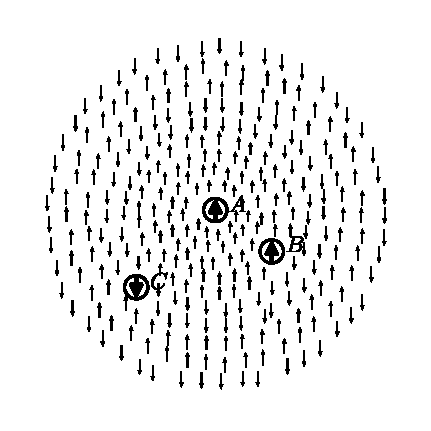
\includegraphics[width=0.72\textwidth]{fig_179.pdf}
\caption*{图 179\quad $s$ 电子围绕杂质 A 的自旋极化 Friedel 振荡，导致与近邻杂质 B 的铁磁性相互作用，但在更远的距离（如 C 处）则可能有利于反铁磁性。}
\end{figure}

这样，我们就有了铁磁性的 Heisenberg 交换模型（§10.4）所需的全部机制：过渡金属离子 $d$ 壳层中局域化的磁矩，由于其极化方向倾向于与浸泡着它们的传导电子气反平行，而被促成为彼此平行。

这类相互作用在稀薄合金中引起复杂的磁学和热学效应，其中磁性离子是无规分布在溶剂晶格上的。在极端情形下，把非磁性溶剂去掉，留下纯过渡金属，这就是诸如 Fe 等金属中铁磁性的 Vonsovski--Zener 模型（Vonsovski--Zener model）。注意，这是一个比 Heisenberg--Dirac 哈密顿量 (10.29) 所提示的“动力学”得多的模型。$d$ 壳层磁矩并不是由整数个完全局域的“d 电子”组成，而是代表 $s$ 带与 $d$ 带已充分杂化的 Bloch 态中的平均贡献。因此，这个模型与 §10.5 中讨论的较简单的能带铁磁性并不矛盾，只是参量 $U$ 需要重新解释。

依赖于自旋的 $s$–$d$ 相互作用 (10.50) 还导致一个与磁性杂质对电阻率的贡献相联系的奇特效应。设我们像 (6.90) 中那样，试图计算这样一个物体把一个处于态 $|\mathbf{k},+\rangle$ 的“向上”自旋 $s$ 电子散射到同自旋态 $|\mathbf{k}',+\rangle$ 的微分截面。

在第一级 Born 近似下，散射振幅恰好就是矩阵元

\begin{align*}
t^{(1)} &= \langle \mathbf{k}, + | \mathcal{H}_{sd} | \mathbf{k}', + \rangle \notag \\
&= -(J/N)\, \mathsf{S}_i^{(z)}. \tag{10.52}
\end{align*}
这一项平方后不为零，而且是价电荷散射等（§7.4）之外的附加项，本来通常就足以满足我们对此问题的好奇心了。

\begin{figure}[H]
\centering
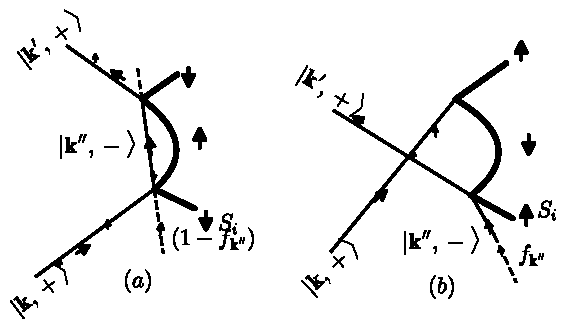
\includegraphics[width=0.72\textwidth]{fig_180.pdf}
\caption*{图 180\quad 二级 $s$–$d$ 散射中的直接过程(a)与交换过程(b)。注意自旋翻转跃迁中 $s$ 自旋与 $d$ 自旋的相对取向。}
\end{figure}

但是，本着一种迂腐的精神，让我们考察微扰级数中更高阶的项。初等量子力学教科书教导我们，第二级 Born 近似取如下形式

\begin{equation*}
t^{(2)} = \sum_{\mathbf{k}'',\sigma} \frac{\langle \mathbf{k}, + | \mathcal{H}_{sd} | \mathbf{k}'', \sigma \rangle \langle \mathbf{k}'', \sigma | \mathcal{H}_{sd} | \mathbf{k}', + \rangle}{\mathcal{E}(\mathbf{k}) - \mathcal{E}(\mathbf{k}'')}, \tag{10.53}
\end{equation*}
其中“中间”态 $|\mathbf{k}'',\sigma\rangle$ 通过相互作用哈密顿量 $\mathcal{H}_{sd}$ 与初态和末态两者相联系。然而，这个表达式并不完全正确。在完整的时间依赖微扰论中，我们必须考虑两类“图”（图 180）。在直接
过程（a）中，入射电子先进入态 $|\mathbf{k}'',\sigma\rangle$（因此该态必须是空的），然后才被发射到末态；而在交换（exchange）过程（b）中，我们假设一个已处于 $|\mathbf{k}'',\sigma\rangle$ 的电子，在“初始”电子被接纳进中间态之前，就先以 $|\mathbf{k}',+\rangle$ 离去。由这些规则，我们应当把 (10.53) 改写成

\begin{align*}
t^{(2)} = \sum_{\mathbf{k}'',\sigma} \frac{1}{\mathcal{E}(\mathbf{k}) - \mathcal{E}(\mathbf{k}'')} \big\{ &(1 - f_{\mathbf{k}''}) \langle \mathbf{k}, + | \mathcal{H}_{sd} | \mathbf{k}'', \sigma \rangle \langle \mathbf{k}'', \sigma | \mathcal{H}_{sd} | \mathbf{k}', + \rangle \\
&+ f_{\mathbf{k}''} \langle \mathbf{k}'', \sigma | \mathcal{H}_{sd} | \mathbf{k}', + \rangle \langle \mathbf{k}, + | \mathcal{H}_{sd} | \mathbf{k}'', \sigma \rangle \big\}, \tag{10.54}
\end{align*}
其中 $f_{\mathbf{k}''}$ 是中间态的占据数。

对于普通的势散射，(10.54) 中两个矩阵元的乘积与其次序无关，于是 $f_{\mathbf{k}''}$ 相消，我们便回到 (10.53)，它对散射截面的贡献只是对一级项 (10.52) 的一个小的修正。但对自旋散射我们必须记住，$\mathcal{H}_{sd}$ 中含有诸如 $\mathsf{S}_i^{(x)} s_x$ 和 $\mathsf{S}_i^{(y)} s_y$ 这样的项，它们以消耗杂质的极化为代价去“翻转”传导电子的自旋（见 (10.104)）。算符 $\mathsf{S}_i^{(x)}$ 与 $\mathsf{S}_i^{(y)}$ 不对易，因此 (10.54) 中各项的先后次序变得重要。从杂质自旋矩的角度看，两个跃迁中哪一个先发生确实至关重要。例如显而易见，倘若杂质已经具有最大的“向上”自旋，直接过程就是被禁戒的。

结果是，在 (10.54) 的代数约化中最终留下一个如下形式的项

\begin{equation*}
t_{\rm K} \approx 2(J/N)^2 \mathsf{S}_i^{(z)} \sum_{\mathbf{k}''} \frac{f_{\mathbf{k}''}}{\mathcal{E}(\mathbf{k}) - \mathcal{E}(\mathbf{k}'')}, \tag{10.55}
\end{equation*}
其中因子 $f_{\mathbf{k}''}$ 并未被来自其他图的贡献所抵消。由于 $f_{\mathbf{k}''}$ 在费米能量处陡然变化，当 $\mathcal{E}(\mathbf{k})$ 趋近 $\mathcal{E}_F$ 时，这个和会变得很大。例如，假设传导带中的态密度一直低到某个能量 $(\mathcal{E}_F - D)$ 都具有 $\mathcal{N}(\mathcal{E}_F)$ 的量级，我们可以把 (10.55) 近似地算成

\begin{equation*}
t_{\rm K} \approx 2(J/N)^2 \mathsf{S}_i^{(z)} \mathcal{N}(\mathcal{E}_F) \ln \frac{D}{|\mathcal{E}_F - \mathcal{E}(\mathbf{k})|}. \tag{10.56}
\end{equation*}
普通带电杂质在金属中产生的\emph{剩余电阻}（residual resistance）与温度无关（§§7.2--7.4）。但是，当我们把磁性杂质引起散射的总概率在费米面上厚度为 $kT$ 的“热层”内积分时，
(10.56) 中的奇性并未因此被抹平。电阻率应当随温度作对数式变化，大致为

\begin{equation*}
\rho(T) \sim \rho_0 \{1 - 2(J/N)\,\mathcal{N}(\mathcal{E}_F) \ln D/kT\}. \tag{10.57}
\end{equation*}

由于 $J$ 本质上是负的，这个公式预言剩余电阻率随温度下降而迅速增大。再把它与基体金属低温下按 $T^5$ 变化的“理想”电阻（§7.5）结合起来，就解释了长期在含过渡元素的稀薄合金中观测到的神秘的电阻极小（resistance minimum）。而 (10.56) 的强能量依赖进入诸如 (7.104) 那样的公式，则解释了在这类材料中同样观测到的巨大温差电功率（giant thermo-electric power）。

但完整的 Kondo 效应（Kondo effect）理论还必须考虑近邻杂质的相互极化、$t$ 的微扰展开的高阶修正、具有 $s$–$d$ 相互作用的系统之基态的性质，以及许多其他微妙之处。这个领域如今已成为固体物理中各种高深量子力学方法的主要演练场之一。

\begin{figure}[H]
\centering
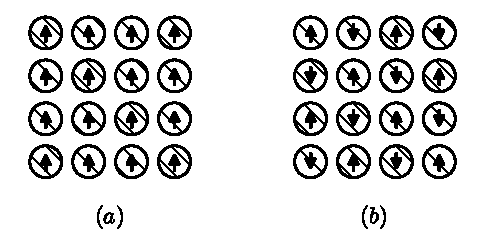
\includegraphics[width=0.72\textwidth]{fig_181.pdf}
\caption*{图 181\quad (a)铁磁有序。(b)反铁磁有序。}
\end{figure}

\section{反铁磁性}

Heisenberg 模型中铁磁性的一般条件是 (10.29) 中的交换积分 $J_{ll'}$ 为正。此时内场与自旋的排列方向平行，整个系统倾向于取图 181(a) 的组态。

但假如——正如对 $J_{ll'}$ 的计算常常表明的那样——该积分的符号为负，那么任一格点上的内场 (10.32) 就会与近邻自旋磁化的平均方向相反，图 181(b) 的排列成为有利。我们把这样的系统称为反铁磁性（antiferromagnetic）的。

为了看出会发生什么，让我们分别考虑自旋取向相反的两套子晶格。设
$\boldsymbol{\mu}_+$ 是 $\oplus$ 子晶格上原子的平均磁化。交换相互作用将在 $\ominus$ 子晶格上产生一个内场（不妨写成）

\begin{align*}
\mathbf{H}^- &= \frac{1}{\beta^2}(\Sigma J)\boldsymbol{\mu}_+ \notag \\
&= \lambda N \boldsymbol{\mu}_+, \tag{10.58}
\end{align*}
这个求和假定只对最近邻进行，因为 $J_{ll'}$ 被认为作用程极短。要点在于，$\lambda$ 现在将是\emph{负}的。

同样由于这一相互作用，每个 $\oplus$ 格点上也存在内场

\begin{equation*}
\mathbf{H}^+ = \lambda N \boldsymbol{\mu}_-. \tag{10.59}
\end{equation*}

现在假设我们的磁体是经典的，即 (10.17) 对磁场 $\mathbf{H}$ 中磁矩 $\boldsymbol{\mu}$ 的\emph{平均}值成立。把 (10.17) 写成

\begin{equation*}
\langle \boldsymbol{\mu} \rangle = \mathcal{L}\{(\boldsymbol{\mu}\cdot\mathbf{H})/kT\}, \tag{10.60}
\end{equation*}
其中用符号 $\mathcal{L}$ 表示由 (10.17) 右端定义的 Langevin 函数（Langevin function）。于是我们有两个方程要求解：

\begin{align*}
\boldsymbol{\mu}_- &= \mathcal{L}\{\boldsymbol{\mu}\cdot(\mathbf{H}+\lambda N\boldsymbol{\mu}_+)/kT\}, \notag \\
\boldsymbol{\mu}_+ &= \mathcal{L}\{\boldsymbol{\mu}\cdot(\mathbf{H}+\lambda N\boldsymbol{\mu}_-)/kT\}. \tag{10.61}
\end{align*}

在高温下，当近似 (10.18) 有效时，这两个方程可以相加而给出 (10.23)。结果与先前的 (10.24) 几乎完全一样：

\begin{equation*}
\chi = \frac{N\langle\mu^2\rangle}{3k(T+\theta)}; \tag{10.62}
\end{equation*}
$\lambda$ 为负时，方便的做法是按 $-\lambda N\langle\mu^2\rangle/3kT$ 来定义 $\theta$，这与 (10.25) 相一致。磁矩倾向于彼此反平行地排列，而不是被磁场拉向同一方向，顺磁磁化率因此减小。

但在低温下，即使不存在磁场也有一个解。若我们写出

\begin{equation*}
\boldsymbol{\mu}_- = -\boldsymbol{\mu}_+ \tag{10.63}
\end{equation*}
（在图 181(b) 的有序反铁磁排列中，直觉上正是如此），则 $\lambda$ 的负号被抵消，我们得到方程

\begin{equation*}
\boldsymbol{\mu}_+ = \mathcal{L}\{(\boldsymbol{\mu}\cdot|\lambda|N\boldsymbol{\mu}_+)/kT\} \tag{10.64}
\end{equation*}
待解。这个方程与 §10.3 中导致铁磁性的方程完全相同——例如 (10.26)，其中含有 Langevin 函数的“量子”等价物。

这样，从单个自旋的角度看，铁磁性与反铁磁性似乎很相似：系统在高温下是顺磁性的，但在某一温度以下变成强极化；在反铁磁情形中，这个温度称为 Néel 温度（Néel temperature），

\begin{equation*}
T_{\rm N} = \theta. \tag{10.65}
\end{equation*}

然而在宏观上，两者的行为大不相同。反铁磁排列不具有任何净极化，因此系统不显示任何永久磁化。所能观测到的只是磁化率的变化；要计算它，需在一个小的磁场 $H$ 之下求解 (10.61)。

\begin{figure}[H]
\centering
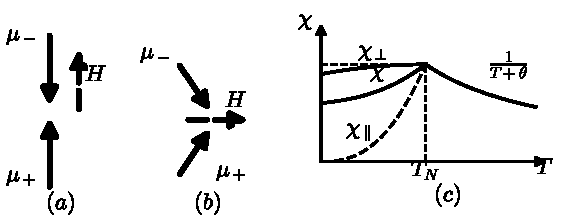
\includegraphics[width=0.72\textwidth]{fig_182.pdf}
\caption*{图 182\quad 反铁磁体的磁化率：(a)$\chi_\parallel$ 趋于零；(b)$\chi_\perp$ 保持恒定；(c)$\chi = \frac{1}{3}\chi_\parallel + \frac{2}{3}\chi_\perp$。}
\end{figure}

这个计算原则上很简单，只是实际做起来略嫌繁琐。其结果有趣之处在于，它依赖于 $\mathbf{H}$ 相对于两套子晶格磁化方向的取向。当 $\mathbf{H}$ 与 $\boldsymbol{\mu}_+$ 平行时，磁化率 $\chi_\parallel$ 在 $T=0$ 处趋于零。这是因为内场强到足以阻止 $\ominus$ 子晶格中的任何自旋翻转。另一方面，$\chi_\perp$ 在 $T=0$ 的值与它在 $T_{\rm N}$ 处应有的值相同：与外场垂直的子晶格极化，对其磁化被稍微转向外场方向只有微弱的抗拒。

实际上，一个宏观样品将包含大量磁畴，各磁畴的极化轴彼此不同，于是对平均磁化率可以写出

\begin{equation*}
\chi = \tfrac{1}{3}\chi_\parallel + \tfrac{2}{3}\chi_\perp. \tag{10.66}
\end{equation*}
$\chi$ 在 $T_{\rm N}$ 处斜率的不连续性很容易观测到，并且与子晶格极化时出现的比热反常相联系。

值得指出的是，由于 $\chi_\perp > \chi_\parallel$，磁场本应能够把所有磁畴都拉成垂直组态。但这种情况并不发生——大概是由于自旋–自旋相互作用的各向异性，它倾向于偏爱某些特殊的晶体方向。

我们在这里考虑的模型，只是展现着令人眼花缭乱的种种现象的一大类系统中的一个简单例子。这个论证可以从不同方向加以细化。例如，晶体结构可能是复杂的，其中磁性离子并不形成简单立方网络，系统究竟会如何划分成子晶格也可能并非一目了然。又如，相互作用的作用程可能比最近邻间更长，或者对某些自旋对是反铁磁性的，而对另一些则是铁磁性的。这样做的一个后果（在我们的框架内很容易处理：只需在 (10.58) 中加上诸如 $\lambda' N\boldsymbol{\mu}_-$ 的项，在 (10.59) 中加上 $\lambda' N\boldsymbol{\mu}_+$ 的项）是改变 Néel 温度，使之不再与 (10.62) 中的参量 $\theta$ 相同。

\begin{figure}[H]
\centering
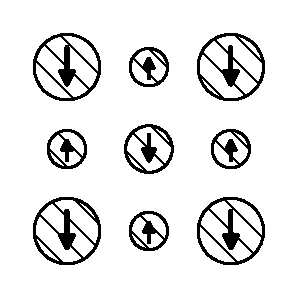
\includegraphics[width=0.72\textwidth]{fig_183.pdf}
\caption*{图 183\quad 亚铁磁性。}
\end{figure}

\begin{figure}[H]
\centering
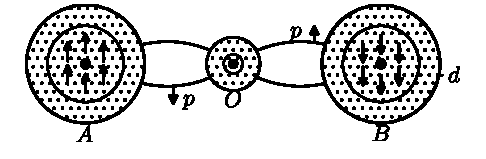
\includegraphics[width=0.72\textwidth]{fig_184.pdf}
\caption*{图 184\quad 超交换。}
\end{figure}

另一种情形是晶体中存在两种不同类型的磁性离子，而且二者不具有相同的磁矩。于是我们可能遇到图 183 所描绘的情况：A、B 两类原子的自旋取向相反，但由于一套子晶格上的矩比另一套上的大，系统仍将显示永久矩。这称为亚铁磁性（ferrimagnetism），是铁氧体（ferrite）的特征；在宏观上，它看起来与铁磁性非常相像。

在许多反铁磁物质中，磁性离子彼此相距相当远，以致很难相信它们能由诸如 (10.37) 那样的交换积分联系起来。这并不意味着晶格非常稀疏，而是意味着在磁性离子之间的空隙里填有许多非磁性离子。例如，它们可以是氧离子，如 MnO 中那样。这时我们就遇到了称为超交换（super-exchange）的机制：Mn 离子中的 $d$ 电子与氧中的电子相耦合，而后者再通过交换作用与第二个 Mn 离子中的 $d$ 电子相互作用。

示意性地，情形可以如图 184 所示。若原子 A 具有 $+$ 自旋，就有空位让一个 $-$ 自旋的电子从氧的 $p$ 态进入。若原子 B 具有 $-$ 自旋，它就能接纳这对电子中来自氧的另一个。这样，氧上 $p$ 电子自旋之间的相互作用就转化为磁性离子 $d$ 壳层自旋之间的相互作用。这一效应的实际计算颇为微妙，但它至少在原理上解释了观测到的现象。

在稀磁合金中，§10.6 的间接交换（indirect exchange）机制也可以是反铁磁性的。如图 179 所示，当第二个杂质恰好处在与第一个磁性离子的 R.K.K.Y. 振荡中“向上”自旋峰相对应的距离上时，就会出现这种情形。但要理解诸如 Cr 这类纯金属中的反铁磁性，我们应当回到 §10.5 的巡游电子图像。

定量地看，不难理解反铁磁图样如何能被传导电子之间的交换作用所稳定。设图 181(b) 那种类型的磁有序已经建立。一个“向上”自旋的电子穿越晶体时，通过交换相互作用 $U$ 将感受到一个依赖于局域极化的有效场。这个场具有磁超晶格的周期性，因而会在通常布里渊区内部的一个“子区”边界上引起能量不连续（参见 §2.6）。能带结构中的这一特征会反映为“向上”自旋电子密度的一个超晶格。对于自旋相反的电子，微扰的符号相反，于是它们倾向于占据另一套超晶格。如果这些分布碰巧与我们最初设想的磁化图样相一致，我们就找到了电子的一种自洽的反铁磁有序，而无须强迫它们局域化。

为了给这类论证赋予数学实质，我们假设
我们把均匀磁化率 (10.42) 推广为一个依赖于 $q$ 的磁响应函数。沿着 §5.1 的思路，在导致磁化率 $\chi_0(\mathbf{q})$（即式 (10.51)）的那类计算中，纳入一个形式如 (10.38) 的交换相互作用是很容易的。所得结果实际上与式 (10.42) 明显相似，即

\begin{equation*}
\chi(\mathbf{q}) = \frac{\chi_0(\mathbf{q})}{1 - \tfrac{1}{2} U (g\beta s)^{-2} \chi_0(\mathbf{q})}.
\tag{10.67}
\end{equation*}

现在，如果这个表达式的分母为零，金属的假定非磁态便是不稳定的。磁有序的 Overhauser 条件是

\begin{equation*}
\tfrac{1}{2} U (g\beta s)^{-2} \chi_0(\mathbf{q}) > 1
\tag{10.68}
\end{equation*}

其中铁磁性的条件 (10.43) 正是 $q = 0$ 的特殊情形。

通常的自由电子间交换相互作用能否在普通金属中导致稳定的自旋密度波（spin density waves），这个问题尚未得到确定的解决。然而在过渡金属中，已知 $U$ 相当大，而待代入 $\chi_0(\mathbf{q})$ 的公式 (10.51) 的电子能态 $\mathcal{E}(\mathbf{k})$ 由能带结构主导。例如，由 §5.4 显然可知，一个横跨费米面相互平行的平坦区域的波矢 $\mathbf{q}$ 可能诱导出很大的 $\chi_0(\mathbf{q})$ 值，从而使 (10.68) 得以满足。在这种情形下，反铁磁有序可能异常复杂：自旋密度的变化等价于锥面上自旋矩的螺旋形排布，其重复距离与底层晶格无关。

\section{Ising 模型}

在讨论铁磁性和反铁磁性时，我们对 Heisenberg 哈密顿量 (10.29) 的态采用了非常粗糙的近似。实际上，我们假定除正在处理的那个自旋之外，每个自旋都取其平均值；我们忽略了相邻格点上自旋之间的涨落与关联。此外，我们还忽略了 $\mathsf{S}_l$ 是算符这一事实——它们不能换成各自的平均期望值。

自旋哈密顿量的本征值分布实际上非常复杂，试图对系统的热力学给出精确的讨论，是固体理论的主要课题之一。这一理论沿两个方向发展。我们可以假定系统接近其基态（铁磁的或反铁磁的），然后讨论低能激发。这就是自旋波（spin waves）理论，将在 §10.11 中概述。

另一类近似是略去自旋算符的非对角元，只考虑它们沿某个固定方向——通常是 $H$ 的方向——的分量。换言之，我们假定系统的能级由下式给出

\begin{equation*}
\mathcal{E} = -\sum_{ll'} J_{ll'} \sigma_l \sigma_{l'} - \beta H \sum_l \sigma_l,
\tag{10.69}
\end{equation*}

\begin{figure}[H]
\centering
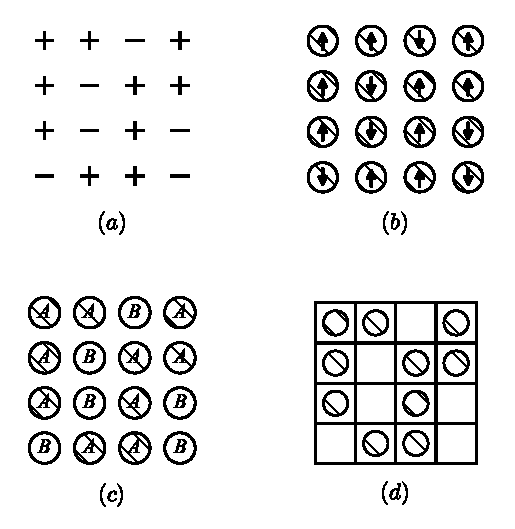
\includegraphics[width=0.72\textwidth]{fig_185.pdf}
\caption*{图 185\quad Ising 模型的一个组态 (a) 可以代表：(b) 自旋的一种排布；(c) 二元合金中原子的一种排布；(d) "格气"的一个组态。}
\end{figure}

其中我们在每个格点 $l$ 上定义一个只能取 $+1$ 或 $-1$ 的“自旋”量子数 $\sigma_l$。在多数情况下我们还假定 $J_{ll'}$ 只在格子中最近邻之间起作用。

这就叫作 Ising 模型。它不可能是铁磁或反铁磁系统的精确描述，但由于它绕开了求自旋集合的精确本征函数这一极为困难的问题，使人们得以集中处理这类系统的态的统计分布这一组合问题。

Ising 模型确实更精确地描述了另一类系统——合金：两种元素 A 和 B 可以在一组固定的格点位置上相互替换。我们可以说 $\sigma_l = +1$ 对应于第 $l$ 个格点上的一个 A 原子，而 $\sigma_l = -1$ 规定该格点上是一个 B 原子。“交换积分” $J$ 这时应解释为

\begin{equation*}
J = \tfrac{1}{2}\bigl\{ \mathcal{V}_{AB} - \tfrac{1}{2}(\mathcal{V}_{AA} + \mathcal{V}_{BB}) \bigr\},
\tag{10.70}
\end{equation*}

其中 $\mathcal{V}_{AB}$ 是相邻格点上 A 原子与 B 原子之间的相互作用能，减去的则是一个 AA 对或一个 BB 对的平均能量。

这类合金系统可以作实验研究，而且发现它们的确表现出一个过渡温度，类似于居里温度或 Néel 温度。在转变点以上，合金是无序的；温度较低时它趋于有序，或者是通过分凝出近乎纯 A 与近乎纯 B 的材料（这对应于 $J > 0$ 的情形，即铁磁性），或者是通过形成 A、B 原子规则地分布在相互穿插的子晶格上的区域——这是反铁磁性的类似物。有序–无序转变（order–disorder transition）与铁磁或反铁磁转变的差别在于：前一情形中 A 类与 B 类原子的总数是固定的，而“向上”与“向下”的自旋却可以自由地相互转变。这一差别在理论上可以形式地加以顾及，因此许多结果对两类系统普遍成立。

Ising 模型可以应用的另一个问题是“格气”（lattice gas）或“格液体”（lattice liquid）问题：把一些能在短距离上相互作用的原子放到一组格点上，并留下空格点。这在形式上与合金问题等价。然而，它是否真正贴切地适用于人们有时让它去描述的液–气转变的热力学，却令人怀疑。

不过，Ising 模型的重要性并不在于描述个别的物理效应；它是一个数学上易于处理的模型，描写一个应当表现出合作现象（co-operative phenomena）和相变的系统。在这个意义上，它更多地属于统计力学的一般理论，而不属于固体理论。然而，有某些原理对晶体格子的一般理论也很重要，我们现在就试图阐明它们。

\section{组合方法}

Ising 模型的优点是，其热力学性质的计算可以归结为一个组合问题。例如，假设我们要求配分函数（partition function）

\begin{equation*}
Z = \sum e^{-\mathcal{E}/kT},
\tag{10.71}
\end{equation*}

其中求和遍及所有“组态”，即遍及格子的 $N$ 个格点上 $+$ 自旋与 $-$ 自旋的各种排布。这个和看起来非常复杂，但形式上它只需涉及两个变量，例如 $N_A$——“向上”自旋[或 A 原子]的数目——与 $N_{AB}$——相邻反平行自旋[或 AB 对]的数目。

为看清这一点，我们把能量 (10.69) 用各种类型的键的总数表出：

\begin{equation*}
\mathcal{E} = J(N_{AB} - N_{AA} - N_{BB}) - \beta H (N_A - N_B).
\tag{10.72}
\end{equation*}

但这些变量并非相互独立。显然有

\begin{equation*}
N_A + N_B = N.
\end{equation*}

同样显然的是，止于 A 格点的键至多只有 $pN_A$ 条，这里 $p$ 是格子的配位数（co-ordination number），即给定格点的最近邻数目。每条这样的键需要在 $N_{AA}$ 中被计及两次、在 $N_{AB}$ 中被计及一次。于是 $2N_{AA} + N_{AB} = pN_A$；类似地 $2N_{BB} + N_{AB} = pN_B$。代入这些条件，我们发现 (10.72) 变成

\begin{equation*}
\mathcal{E} = -\tfrac{1}{2} pNJ + 2N_{AB} J - (2N_A - N)\beta H.
\tag{10.73}
\end{equation*}

现在设 $g(N; N_A, N_{AB})$ 表示把 $N_A$ 个“向上”自旋放到格子上、且恰有 $N_{AB}$ 对反平行近邻的全部放法数。所有这些组态都具有相同的能量；我们可以把配分函数 (10.71) 写成

\begin{align*}
Z &= y^{\frac{1}{2}N} z^{-\frac{1}{2}pN} \sum_{N_A, N_{AB}} g(N; N_A, N_{AB})\, y^{N_A} z^{N_{AB}} \\
&= y^{\frac{1}{2}N} z^{-\frac{1}{2}pN} \Lambda_N(y, z),
\tag{10.74}
\end{align*}

其中变量 $y$ 和 $z$ 与磁场及相互作用 $J$ 相联系：

\begin{equation*}
y \equiv e^{2\beta H/kT}; \quad z \equiv e^{-2J/kT}.
\tag{10.75}
\end{equation*}

系统的全部有趣性质现在都集中在函数 $\Lambda_N$ 之中；由它可以导出适用于“铁磁”与“反铁磁”系统、或合金相与正规溶液（regular solutions）理论的公式。

但是，计算 (10.74) 中组合因子的问题一般是不可解的；已知的只是近似公式。对给定的 $N_A$ 值，算出组态的总数并不困难。由初等代数，这必是把 $N_A$ 个物体放到 $N$ 个位置上的排布方式总数

\begin{equation*}
\sum_{N_{AB}} g(N; N_A, N_{AB}) = \frac{N!}{N_A! (N - N_A)!}.
\tag{10.76}
\end{equation*}

困难在于把这个总数按 $N_{AB}$ 的各个取值分开。

一个非常粗糙的近似，是把对 $N_{AB}$ 的单独求和换成假定它取其平均值。也就是说，我们把 $N_A$ 个 A 原子和 $N_B$ 个 B 原子无规地分布在格子的格点上，并计算 $\tfrac{1}{2}pN$ 条键中任一条一端为 A 原子、另一端为 B 原子的概率。结果当然是

\begin{align*}
\langle N_{AB} \rangle &= 2\, \frac{N_A}{N}\, \frac{N_B}{N}\, \tfrac{1}{2} pN \\
&= \frac{p N_A N_B}{N}.
\tag{10.77}
\end{align*}

把 (10.76) 和 (10.77) 代入 (10.74)，得

\begin{equation*}
\Lambda_N \approx \sum_{N_A} \frac{N!}{N_A! N_B!}\, y^{N_A} z^{p N_A N_B / N}.
\tag{10.78}
\end{equation*}

由此可以计算自由能：从对数中取出最大的项，并用 Stirling 公式作渐近展开。于是

\begin{align*}
F &= -kT \ln \Lambda_N \\
&\approx kT \Bigl\{ -N \ln N + N_A \ln N_A + N_B \ln N_B - N_A \ln y - p\, \frac{N_A N_B}{N} \ln z \Bigr\}.
\tag{10.79}
\end{align*}

\begin{figure}[H]
\centering
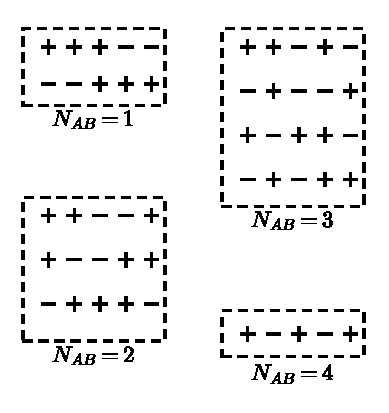
\includegraphics[width=0.72\textwidth]{fig_186.pdf}
\caption*{图 186\quad 对 $N=5$、$N_A=3$ 的链作组态计数。此系统的 $\langle N_{AB}\rangle = 2.4$。}
\end{figure}

自由能取极小（也即求和中出现极大项）的条件，可通过对 $N_A$ 求导得到（当然要取 $N_B = N - N_A$）。利用 (10.75)，我们得到

\begin{equation*}
\ln N_A - \ln N_B - \frac{2\beta H}{kT} - \frac{(N_A - N_B)}{N}\, \frac{2pJ}{kT} = 0,
\end{equation*}

即

\begin{equation*}
\frac{N_A}{N_B} = \exp \Bigl\{ \frac{2\beta H}{kT} + \Bigl( \frac{N_A - N_B}{N} \Bigr) \frac{2pJ}{kT} \Bigr\},
\tag{10.80}
\end{equation*}

或

\begin{equation*}
\Bigl( \frac{N_A - N_B}{N} \Bigr) = \tanh \Bigl\{ \frac{\beta H}{kT} + \Bigl( \frac{N_A - N_B}{N} \Bigr) \frac{pJ}{kT} \Bigr\}.
\tag{10.81}
\end{equation*}

如果把 $(N_A - N_B)/N$ 认作 $\langle \mu \rangle$，即系统的平均净极化，并像 (10.33) 那样把 $pJ$ 表为一个内场，那么我们就回到了铁磁转变的居里–外斯条件 (10.26)。在合金理论中，这被称为 Bragg--Williams 近似（Bragg--Williams approximation）。

\begin{figure}[H]
\centering
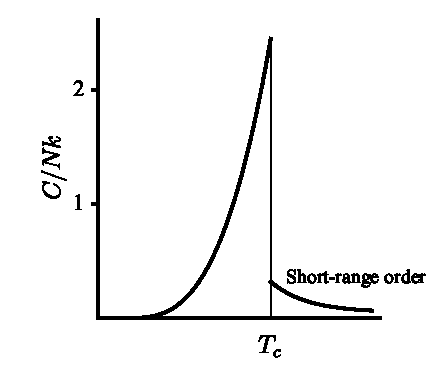
\includegraphics[width=0.72\textwidth]{fig_187.pdf}
\caption*{图 187\quad 准化学近似下的比热，格子的配位数为 p = 12。}
\end{figure}

上面这个初等内场公式的推导暴露了它的局限性；它对相邻自旋之间的关联只字未提。例如在铁磁体中，由于自旋对有平行排列的倾向，我们可以预期随机平均值 (10.77) 高估了实际平衡组态中 AB 对的数目。

改进这一点的一个有趣途径是 Guggenheim 的准化学近似（quasi-chemical approximation）。假设我们在无规混合的基础上算出与 (10.77) 类似的其他平均值，就得到

\begin{equation*}
\frac{\langle N_{AB} \rangle^2}{\langle N_{AA} \rangle \langle N_{BB} \rangle} = 4.
\tag{10.82}
\end{equation*}

但如果我们处理的是分子之间的化学平衡，如同化学反应

\begin{equation*}
AA + BB \rightleftharpoons 2AB,
\tag{10.83}
\end{equation*}

所表达的那样，那么我们知道，不同组元的平衡浓度应由下式给出

\begin{equation*}
\frac{\langle N_{AB} \rangle^2}{\langle N_{AA} \rangle \langle N_{BB} \rangle} = 4\, \frac{\bigl( e^{-\mathcal{E}_{AB}/kT} \bigr)^2}{e^{-\mathcal{E}_{AA}/kT}\, e^{-\mathcal{E}_{BB}/kT}},
\tag{10.84}
\end{equation*}

其中 $\mathcal{E}_{AB}$ 等等是 AB 分子等等的能量。用 (10.75) 的记号，这提示 (10.84) 的右端平均而言应等于 $4z^2$。对 (10.73) 稍作变换，便可算出 $\langle N_{AB} \rangle$，并用它代替 (10.77) 放入 (10.78)。

这个计算我们就不再往下做了，只想指出：在由下式定义的转变温度以下，系统表现出自发极化（铁磁性或反铁磁性）

\begin{equation*}
\frac{kT_c}{pJ} = \frac{2/p}{\ln(1 - 2/p)},
\tag{10.85}
\end{equation*}
（译注：按准化学近似的标准结果，右端应为 $-2/p\big/\ln\frac{p}{p-2}$，原书疑漏负号。）

在配位数 $p$ 很大的极限下，它应趋于 (10.28)（在我们现在的记号中 $k\theta = pJ$）。我们还可以近似地计算转变温度附近的比热；它表现出一个尖锐的奇点，在高温一侧有一间断，如图 187 所示。

碰巧，准化学近似等价于另一个看上去颇不相同的方法，它出自 Bethe 和 Peierls。这是把内场论证加以推广的一种尝试。取一个自旋集团——例如中心一个位于 $l = 0$ 的自旋，以及它的 $p$ 个近邻。从这个集团的能量中取 (10.69) 的下列各项：

\begin{equation*}
\mathcal{E}_p = -\sum_{j=1}^{p} J \sigma_0 \sigma_j - \beta H \sigma_0 - \beta H_I \sum_{j=1}^{p} \sigma_j.
\tag{10.86}
\end{equation*}

换言之，我们假定中心自旋感受到实际的外场 $H$，并且显式地与近邻的自旋相连；而对集团的外围格点，我们则假定可以把它们与环境的相互作用当作一个内场 $H_I$ 的效应来处理。

\begin{figure}[H]
\centering
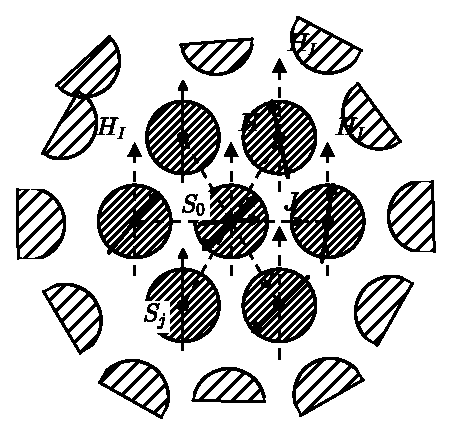
\includegraphics[width=0.72\textwidth]{fig_188.pdf}
\caption*{图 188\quad Bethe–Peierls 集团。}
\end{figure}

很容易为这个集团写出完整的配分函数，因为它只含 $p$ 项。于是可以算出集团中心原子的平均取向。但中心格点并不是格子中什么特权位置；$\langle \sigma_0 \rangle$ 必须与 $\langle \sigma_j \rangle$ 相同，后者是集团边缘上一个自旋的平均矩，它同样可以写成 $H_I$ 的函数。这就给出了内场 $H_I$ 的一个自洽条件：即使 $H = 0$，在低于由 (10.75) 定义的转变温度 $T_c$ 的温度下，$H_I$ 也可以不为零。

Bethe 方法作为一种物理上直观的程序是有吸引力的，甚至可以让它对更现实的模型给出结果：引入真正的自旋算符来代替 (10.86) 的“Ising 自旋变量”，并对这个集团哈密顿量的能级计算配分函数。或者，我们也可以在第一近邻的简单集团之外再引入更多的壳层，把问题解到更高的近似。

这些更高阶的近似，实际上是想更准确地确定 $\Lambda_N(y, z)$ 幂级数展开的系数。可以证明，每一个系数——无论是低温下有效的按 $z$ 的幂的展开，还是高温下有效的按

\begin{equation*}
w = \tanh \frac{J}{kT},
\tag{10.87}
\end{equation*}

的幂的展开——都依赖于数出在格子的“键”上能够描出的、具有给定边数的多边形，这颇像非理想气体理论中的 Mayer 集团和展开，或微扰论中的“图形”。这种计数原则上足够容易，实际做起来却极其繁难。

此外，这样的展开还不能完全使人相信：系统在某个确定温度的热力学性质中真的存在奇点；而 Bragg--Williams 方法和 Bethe 方法的封闭解析公式也填补不了这个空缺。这些方法\emph{假定}存在一个内场，或者假定系统有一个平均说来在每个格点上都相同的净极化。换言之，它们假定系统具有长程序（long-range order）——也就是说，只要知道一个格点上自旋的方向，我们就能猜出任何其他格点上它的方向，不管有多远。\footnote{在铁磁情形，要知道整个格子极化的净方向，只需知道一个自旋。在反铁磁情形，远处格点上自旋的方向当然还取决于它是否与原点的格点属于同一个子晶格。}

\begin{figure}[H]
\centering
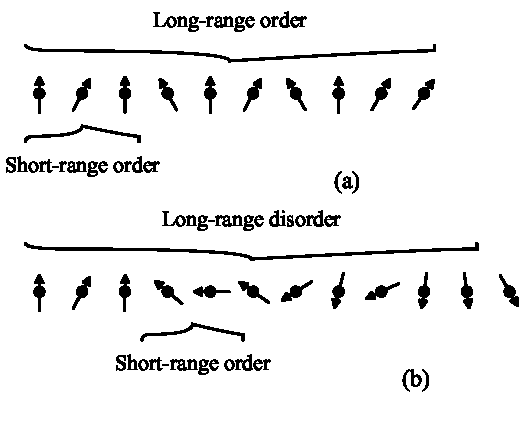
\includegraphics[width=0.72\textwidth]{fig_189.pdf}
\caption*{图 189\quad (a) 长程序蕴含短程序。(b) 短程序并不蕴含长程序。}
\end{figure}

我们前面已经指出，Bragg--Williams 方法甚至给不出任何短程序（short-range order），除非它是被假定的长程序所蕴含的：在居里温度以上，分布被假定得完全无规，每个自旋都与近邻的详细行为无关。Bethe 方法在 $T_c$ 以上会给出短程序，因此更为现实。两种方法都能相当好地描述长程有序态在充分建立之后的一般性质，但都不能用来证明这个态的确存在。

\section{Ising 问题的严格解}

事实证明，Ising 问题可以在两种特殊情形下严格求解。其中一种情形是平庸的，证明也很简单；另一种情形表述起来并不困难，但配分函数最终公式的证明却太过艰难，无法在这里给出。

平庸的情形是线性链；我们给出它的解，因为它展示了一种普遍的技巧。设考虑由 $N$ 个“层”组成的格子。在一维情形，这样一个“层”就是单个格点；在二维情形，它会是完整的一行原子，依此类推。

现在设 $\nu_j$ 是标志第 $j$ 层“状态”的记号；例如在二维情形，$\nu_j$ 可以是 $(++-+\ldots)$ 这样的符号，它给出第 $j$ 行中所有原子的自旋方向。我们假设只有相邻的层之间才有相互作用，即能量可以写成

\begin{equation*}
\mathcal{E} = \sum_{j=1}^{N} \mathcal{V}(\nu_j, \nu_{j+1}) + \sum_{j=1}^{N} \mathcal{V}(\nu_j)
\tag{10.88}
\end{equation*}

（其中包括每一层的“内能”，并且像 §1.6 中那样把两端闭合起来，使得 $\nu_{N+1} \equiv \nu_1$）。

于是系统的配分函数可以写成

\begin{equation*}
Z = \sum_{\nu_1}\sum_{\nu_2}\cdots\sum_{\nu_N}\left\{\prod_{j=1}^{N}\exp\left[-\left[\mathcal{V}(\nu_j, \nu_{j+1}) + \tfrac{1}{2}\mathcal{V}(\nu_j) + \tfrac{1}{2}\mathcal{V}(\nu_{j+1})\right]/kT\right]\right\}.
\tag{10.89}
\end{equation*}

但这不过相当于写下一串矩阵的乘积，其典型元素是

\begin{equation*}
P_{\nu_j\nu_{j+1}} = \exp\left\{-\left[\mathcal{V}(\nu_j, \nu_{j+1}) + \tfrac{1}{2}\mathcal{V}(\nu_j) + \tfrac{1}{2}\mathcal{V}(\nu_{j+1})\right]/kT\right\},
\tag{10.90}
\end{equation*}

这里要认识到，$\nu_j$ 是一个记号，按照层的复杂程度，它可以取两个或更多的值。实际上，式 (10.89) 说的无非是

\begin{align*}
Z &= \mathrm{trace}\,(P^N)\\
&= \sum_i \lambda_i^N,
\tag{10.91}
\end{align*}

其中 $\lambda_i$ 是式 (10.90) 中矩阵 $P$ 的本征值。实际上我们是假定 $N$ 很大——即我们的链几乎无限长——所以只有 $P$ 的最大本征值才是重要的。于是有结果

\begin{align*}
F &= -kT\ln Z\\
&\to -NkT\ln\lambda_{\max},
\tag{10.92}
\end{align*}

这表明自由能是一种广延性质。

现在，在一维链中，记号 $\nu_j$ 正是 $\sigma_j$ 的取值 $+1$ 和 $-1$。矩阵 (10.90) 可以写成

\begin{equation*}
P = \begin{pmatrix}\, y^{-\frac{1}{2}}z^{-\frac{1}{2}} & z^{\frac{1}{2}}\,\\[2pt]\, z^{\frac{1}{2}} & y^{\frac{1}{2}}z^{-\frac{1}{2}}\, \end{pmatrix}
\tag{10.93}
\end{equation*}

（用 (10.75) 的记号）。这个矩阵的本征值是

\begin{equation*}
\lambda_{\pm} = \tfrac{1}{2}\left\{(1+y) \pm \sqrt{\left[(1-y)^2 + 4yz^2\right]}\,\right\} y^{-\frac{1}{2}}z^{-\frac{1}{2}};
\tag{10.94}
\end{equation*}

把 $\lambda_+$ 代入 (10.92)，我们的问题便告解决。

这个结果的有趣之处在于，$F$ 既是 $y$ 的连续函数，又是 $z$ 的连续函数——也就是说，它是 $H$ 和 $T$ 的连续函数，没有奇点。零场下的比热可以算出，就是

\begin{equation*}
C_v = Nk\left(\frac{J}{kT}\right)^{2}\mathrm{sech}^2\left(\frac{J}{kT}\right),
\tag{10.95}
\end{equation*}

它在 $kT = J$ 附近有一个平滑的极大，但不表现出相变。

此外，在 $H = 0$ 时不存在与自发磁化强度相对应的解。\emph{线性链不是铁磁性的}。这一点从 Bragg--Williams 公式 (10.81) 本来看不出来，但在 Bethe 方法中确实显露出来：按式 (10.85)，当配位数 $p$ 趋于 2 时 $T_c \to 0$。当然，同样的结论对反铁磁性也成立。

\begin{figure}[H]
\centering
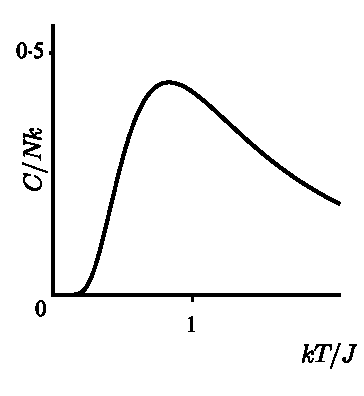
\includegraphics[width=0.72\textwidth]{fig_190.pdf}
\caption*{图 190\quad 线性链的比热。}
\end{figure}

重要的是要认识到这是一条\emph{拓扑}定理；Bethe 方法中 $p = 2$ 给不出转变温度这一点很可能只是偶然的。关键在于，线性链在任意一点都太容易被弄断。引入一个断口，便摧毁了长程序，使能量增加 $2J$；但断口可以出现在 $N$ 个格点中的任何一处，于是熵增加了 $k\ln N$。自由能的改变将会是

\begin{equation*}
F = 2J - kT\ln N,
\tag{10.96}
\end{equation*}

\begin{figure}[H]
\centering
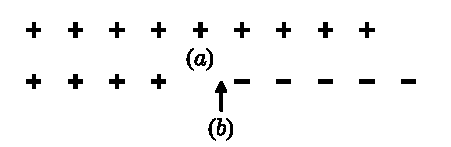
\includegraphics[width=0.72\textwidth]{fig_191.pdf}
\caption*{图 191\quad 线性链中的长程序 (a) 被单个断口 (b) 破坏。}
\end{figure}

只要 $N$ 足够大，无论温度多低，它总可以被做成负的。由这个论证——或者由对一个像 (10.93) 那样的矩阵的本征值所作的更精细的讨论，该矩阵阶数有限而且所有元素都为正——可以推断：任何只在一个维度上无限的格子都将没有奇点。这是“一条链构不成晶体”这条格言的一个典型例证；凡研究凝聚态的学生都应当把它牢牢记在心头。

不难证明，在二维格子中上述反驳不再成立。例如，假设我们造出一个反转自旋的连通区域，如图 192 所示。这个区域将由一条长度为 $L$ 的多边形边界围住——也就是说，在两个区域之间的边界上将有 $L$ 条 AB 型的连键。于是系统的能量将增加 $2LJ$。但与这份能量相联系的熵是多少？一般地说，边界的每个节点处有 3 个可供选择的方向，因此铺排这条边界的方式约有 $3^L$ 种。实际上这是高估，因为多边形还必须重新闭合——但当 $L$ 很大时这个误差并不重要。于是，对自由能的贡献将是

\begin{align*}
F &\approx 2LJ - kT\ln 3^L\\
&= L(2J - kT\ln 3).
\tag{10.97}
\end{align*}

\begin{figure}[H]
\centering
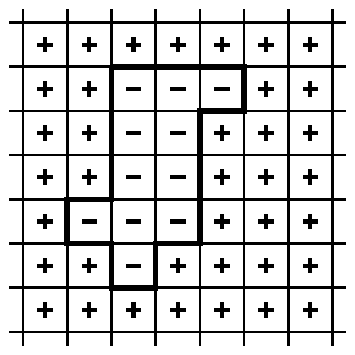
\includegraphics[width=0.72\textwidth]{fig_192.pdf}
\caption*{图 192\quad 一个反转自旋的区域。}
\end{figure}

如果

\begin{equation*}
kT < \frac{2J}{\ln 3},
\tag{10.98}
\end{equation*}

则所有这类贡献都将为正。

有序态在这个温度以下应当是稳定的。

这个粗糙的论证可以由严格的计算来支持，因为 Ising 模型另一个可解的情形是二维正方格子。Onsager 证明了该系统在温度

\begin{equation*}
kT_c = \frac{2J}{\ln(1+\sqrt{2})}
\tag{10.99}
\end{equation*}

以下是“铁磁性的”（或“反铁磁性的”）；这一证明所要求的代数定理远远超出我们现在的范围（尽管其出发点实际上就是式 (10.92) 所引述的关系）。

这个结果最有趣的特征是：虽然自由能本身是温度的连续函数，比热却在居里温度两侧对数式地发散。这样的奇点实际上在任何固态体系中都没有观察到，但这也许是因为我们不容易真正实现一个二维的 Ising 自旋集合。

\begin{figure}[H]
\centering
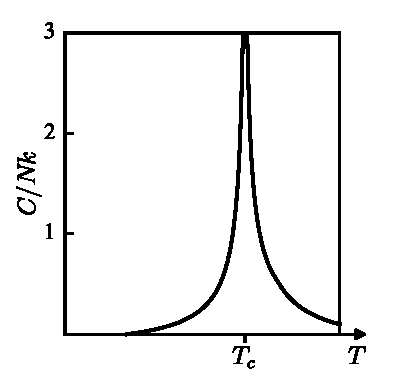
\includegraphics[width=0.72\textwidth]{fig_193.pdf}
\caption*{图 193\quad 正方层格的比热：Onsager 公式。}
\end{figure}

Onsager 方法还可以应用于另外几种二维格子，它们表现出类似的性质；此外还有一些优美的拓扑定理，利用它们可以在其他情形下定出转变温度。然而，对于处在有限磁场中的二维 Ising 铁磁体，不存在严格解。

对三维格子来说，Ising 问题完全没有严格解。人们可以有把握地相信它们会表现出长程序，因为拓扑条件比二维更有利于合作效应；借助级数展开，居里点可以定得相当准确。

由这段讨论产生一条重要原理。按照 Bethe 方法，有序–无序转变应当只依赖于配位数 $p$（参看式 (10.75)）。这样一来，二维三角格子与三维简立方格子的配位数都是 $p = 6$，二者就应当有完全相同的性质。事实上，它们的行为大不相同：比热曲线不同，转变温度也不同。格子的维数对合作现象是带根本性的，实际上对固体的许多性质也是如此。

\begin{figure}[H]
\centering
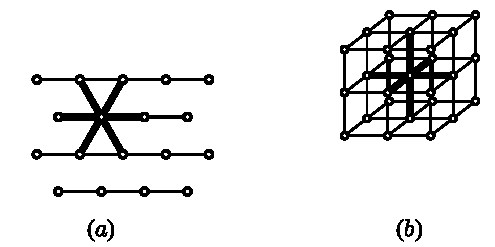
\includegraphics[width=0.72\textwidth]{fig_194.pdf}
\caption*{图 194\quad 三角层格 (a) 与简立方格子 (b) 具有相同的配位数。}
\end{figure}

\section{自旋波}

让我们回到自旋哈密顿量 (10.29)，并假定交换积分为铁磁型的。在零磁场中

\begin{equation*}
\mathcal{H} = -\sum_{ll'} J_{ll'}\,\mathsf{S}_l \cdot \mathsf{S}_{l'}.
\tag{10.100}
\end{equation*}

设 $S$ 是每个离子的总自旋。我们可以用自旋的 $z$ 分量 $\mathsf{S}_l^z$ 的本征态来给第 $l$ 个离子上的自旋态分类。于是，对沿 $z$ 方向分量为 $S'$ 的态

\begin{equation*}
\mathsf{S}_l^z\left|S'\right\rangle_l = S'\left|S'\right\rangle_l
\tag{10.101}
\end{equation*}

（本节中取 $\hbar = 1$）。

铁磁性普遍理论的假定是：哈密顿量 $\mathcal{H}$ 有这样一个基态，其中所有自旋都沿 $z$ 方向最大限度地排列。我们假定这个态可以写成

\begin{equation*}
\left|0\right\rangle = \left|S\right\rangle_1\left|S\right\rangle_2\left|S\right\rangle_3\ldots\left|S\right\rangle_l\ldots\left|S\right\rangle_N,
\tag{10.102}
\end{equation*}

其中 $\mathsf{S}^z$ 在格子的每个格点上都取其最大值 $S$。

容易验证这是 $\mathcal{H}$ 的一个本征态。让我们为某一格点上的自旋定义两个新算符（暂时略去它的标记 $l$）

\begin{equation*}
\mathsf{S}^{+} \equiv \mathsf{S}^{x} + i\mathsf{S}^{y}, \quad \mathsf{S}^{-} \equiv \mathsf{S}^{x} - i\mathsf{S}^{y}.
\tag{10.103}
\end{equation*}

它们是自旋偏离（spin-deviation）算符。例如，考察一下用 $\mathsf{S}^{+}$ 作用到 $\mathsf{S}^z$ 的一个本征态上的效果；其结果是 $\mathsf{S}^z$ 的另一个本征态。于是，采用 (10.101) 的记号，

\begin{align*}
\mathsf{S}^z\{\mathsf{S}^{+}\left|S'\right\rangle\} &= \mathsf{S}^z(\mathsf{S}^{x}+i\mathsf{S}^{y})\left|S'\right\rangle\\
&= \{(\mathsf{S}^{x}\mathsf{S}^z+i\mathsf{S}^{y})+i(\mathsf{S}^{y}\mathsf{S}^z-i\mathsf{S}^{x})\}\left|S'\right\rangle\\
&= \mathsf{S}^{+}\mathsf{S}^z\left|S'\right\rangle+\mathsf{S}^{+}\left|S'\right\rangle\\
&= \mathsf{S}^{+}(S'+1)\left|S'\right\rangle\\
&= (S'+1)\{\mathsf{S}^{+}\left|S'\right\rangle\},
\tag{10.104}
\end{align*}

这里用了自旋算符的熟知对易关系。这样，$\mathsf{S}^{+}\left|S'\right\rangle$ 是 $\mathsf{S}^z$ 的本征值为 $S'+1$ 的本征态——换句话说，它就是态 $\left|S'+1\right\rangle$。$\mathsf{S}^{+}$ 的效果是使自旋在 $z$ 方向上的分量增加一个单位。类似地，$\mathsf{S}^{-}$ 使 $S'$ 减少一个量子。

\begin{figure}[H]
\centering
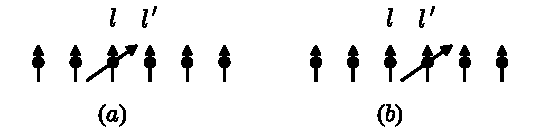
\includegraphics[width=0.72\textwidth]{fig_195.pdf}
\caption*{图 195\quad 算符 $\mathsf{S}_l^{\dagger}\mathsf{S}_{l'}^{-}$ 交换自旋偏离。}
\end{figure}

把 (10.103) 代入哈密顿量是很容易的事，后者可以写成

\begin{equation*}
\mathcal{H} = -\sum_{ll'} J_{ll'}\{\mathsf{S}_l^z\mathsf{S}_{l'}^z + \tfrac{1}{2}(\mathsf{S}_l^{+}\mathsf{S}_{l'}^{-}+\mathsf{S}_l^{-}\mathsf{S}_{l'}^{+})\}.
\tag{10.105}
\end{equation*}

当 $\mathcal{H}$ 作用在态 (10.102) 上时，只有 $z$ 分量作出贡献：

\begin{equation*}
\mathcal{H}\left|0\right\rangle = -\sum_{ll'} J_{ll'}S^2\left|0\right\rangle.
\tag{10.106}
\end{equation*}

算符 $\mathsf{S}_l^{+}$ 作用在态 $\left|S\right\rangle_l$ 上给出零，因为我们不能把 $\mathsf{S}_l^z$ 的本征值增大到超过它的最大值 $S$。于是，有序态 $\left|0\right\rangle$ 是总哈密顿量的本征态。

但现在来考虑系统的激发。自然而然的设想是，它们对应于单个自旋发生偏离的态，如图 195(a) 那样。然而，这样的态并不是 $\mathcal{H}$ 的本征态；算符 $\mathsf{S}_l^{+}\mathsf{S}_{l'}^{-}$ 作用在这个态上，会把它变成另一个态，如图 195(b) 那样，自旋偏离已经被交换到它的近邻身上。Ising 模型中所用的那种态的分类（例如图 185）在这里行不通；自旋偏离会在格子中不停地四处游走。

这种交换效应颇像 Bloch 态的紧束缚模型（§3.4）中电子从一个原子被递交给下一个原子的过程，而且结果证明它具有非常相似的数学性质。这一效应的数学表述如下。

让我们设 $S$ 是一个相当大的数（比如 $\frac{5}{2}$）。$\mathsf{S}^{-}$ 的效果是“产生一个自旋偏离”。我们不采用 (10.101) 的分类，而写

\begin{equation*}
n = S - S',
\tag{10.107}
\end{equation*}

并把态 $\left|n\right\rangle$ 定义为带有 $n$ 个自旋偏离量子的态。只要 $n < 2S$，我们就有通过 $\mathsf{S}^{-}$ 和 $\mathsf{S}^{+}$ 的作用来产生和湮没这些量子的自由。因此，这些算符带有简谐振子的常规理论中湮没算符和产生算符的某些性质（参看 §2.11）。

为了形式地表明这一点，我们可以计算对易子

\begin{align*}
[\mathsf{S}^{+},\mathsf{S}^{-}] &= i[\mathsf{S}^{y},\mathsf{S}^{x}] - i[\mathsf{S}^{x},\mathsf{S}^{y}]\\
&= -2i(i\mathsf{S}^z)\\
&= 2\mathsf{S}^z.
\tag{10.108}
\end{align*}

于是，若令

\begin{equation*}
a = \frac{\mathsf{S}^{+}}{(2\mathsf{S}^z)^{\frac{1}{2}}}, \quad a^{*} = \frac{\mathsf{S}^{-}}{(2\mathsf{S}^z)^{\frac{1}{2}}},
\tag{10.109}
\end{equation*}

则 $a$ 和 $a^{*}$ 具有标准的对易关系

\begin{equation*}
[a, a^{*}] = 1,
\tag{10.110}
\end{equation*}

而且互为复共轭。

定义 (10.109) 没有指明 $\mathsf{S}^{+}$ 和 $[\mathsf{S}^z]^{-\frac{1}{2}}$ 究竟应当按什么次序取——由于这些算符互不对易，这本来可能造成严重的后果。但若 $S$ 足够大，我们就可以忽略这个误差，把算符 $2\mathsf{S}^z$ 换成数 $2S$，因为我们只打算考虑几乎完全排列整齐的态。在这个近似下，自旋偏离态 $\left|n\right\rangle$ 是 $a^{*}a$ 的本征态，我们可以写

\begin{equation*}
a\left|n\right\rangle = n^{\frac{1}{2}}\left|n-1\right\rangle, \quad a^{*}\left|n\right\rangle = (n+1)^{\frac{1}{2}}\left|n+1\right\rangle.
\tag{10.111}
\end{equation*}

$n$ 的定义还意味着我们可以写

\begin{equation*}
\mathsf{S}^z = S - a^{*}a.
\tag{10.112}
\end{equation*}

现在把 (10.109) 和 (10.112) 代入哈密顿量 (10.105)。它近似地变成

\begin{align*}
\mathcal{H} &\approx -\sum_{ll'} J_{ll'}\{(S-a_l^{*}a_l)(S-a_{l'}^{*}a_{l'})+\tfrac{1}{2}\cdot 2S(a_l^{*}a_{l'}+a_l a_{l'}^{*})\}\\
&\approx -\sum_{ll'} J_{ll'}\{S^2 + S(a_l a_{l'}^{*}+a_l^{*}a_{l'}-a_l^{*}a_l-a_{l'}^{*}a_{l'})\},
\tag{10.113}
\end{align*}

这里我们略去了一个 $a_l^{*}a_l a_{l'}^{*}a_{l'}$ 量级的项。

式 (10.113) 中的第一项就是基态（式 (10.116)；译注：疑为 (10.106) 之误印）的能量；其余各项是算符，明确地表达自旋偏离从一个格点向下一个格点的传递。这颇像晶格动力学中的情形——晶格位移依靠弹性力从一个格点传到另一个格点——或者，正如我们已指出过的，像电子波的紧束缚公式。我们可以用在 §2.1 中用过的同一手法求出这个哈密顿量的本征态：代入

\begin{equation*}
a_l = N^{-\frac{1}{2}}\sum_{\mathbf{q}} a_{\mathbf{q}}\,e^{i\mathbf{q}\cdot\mathbf{l}}, \quad a_l^{*} = N^{-\frac{1}{2}}\sum_{\mathbf{q}} a_{\mathbf{q}}^{*}\,e^{-i\mathbf{q}\cdot\mathbf{l}},
\tag{10.114}
\end{equation*}

来代替每个格点上的湮没算符和产生算符。这等价于 (2.8)；波矢 $\mathbf{q}$ 满足与晶格动力学中相同的条件，而新算符 $a_{\mathbf{q}}$ 和 $a_{\mathbf{q}}^{*}$ 满足对易关系 (10.110)。

把 (10.114) 代入 (10.113)，并利用 $J_{ll'}$ 只依赖于 $\mathbf{h} = \mathbf{l}-\mathbf{l}'$ 这一事实（如 (2.6) 中那样），我们得到

\begin{equation*}
\mathcal{H} = \mathcal{H}_0 + \sum_{\mathbf{q}}\left\{\sum_{\mathbf{h}} 2SJ(\mathbf{h})\left(1-e^{-i\mathbf{q}\cdot\mathbf{h}}\right)\right\}a_{\mathbf{q}}^{*}a_{\mathbf{q}},
\tag{10.115}
\end{equation*}

其中 $\mathcal{H}_0$ 与算符 $a_{\mathbf{q}}$ 无关。但 $\mathcal{H}-\mathcal{H}_0$ 是一组简谐振子的哈密顿量，每个波矢 $\mathbf{q}$ 对应一个振子，每个振子具有能级

\begin{equation*}
\mathcal{E}_{\mathbf{q}} = n_{\mathbf{q}}\sum_{\mathbf{h}} 2SJ(\mathbf{h})\left(1-e^{-i\mathbf{q}\cdot\mathbf{h}}\right).
\tag{10.116}
\end{equation*}

换句话说，算符 $a_{\mathbf{q}}$、$a_{\mathbf{q}}^{*}$ 是自旋波的湮没算符和产生算符，自旋波是系统的元激发。第 $\mathbf{q}$ 个自旋波模中的能量以下列量子为单位而量子化：

\begin{equation*}
\hbar\omega_{\mathbf{q}} = \sum_{\mathbf{h}} 2SJ(\mathbf{h})\left(1-e^{-i\mathbf{q}\cdot\mathbf{h}}\right).
\tag{10.117}
\end{equation*}

仿照光子、声子和等离激元的命名，这样的元激发有时叫作磁振子（magnon）。

对于只含最近邻相互作用的简单格子，式 (10.117) 在小波矢下的形式容易算出：

\begin{equation*}
\hbar\omega_{\mathbf{q}} \approx 2SJq^2a^2,
\tag{10.118}
\end{equation*}

其中 $a$ 是晶格常数。于是，磁振子的能量正比于其波矢的平方——颇像电子的能量。实际上，可以定义一个“有效质量” $m^{*}$，使得

\begin{equation*}
\hbar\omega_{\mathbf{q}} \approx \frac{\hbar^2 q^2}{2m^{*}}.
\tag{10.119}
\end{equation*}

对于居里温度为几百开的典型铁磁体（由此可从式 (10.34) 得出 $J$ 的量级），我们发现 $m^{*}$ 约为自由电子质量的 10 倍。

激发谱的形式带来若干简单的推论。例如，由于磁振子服从 Bose--Einstein 统计，可以用 (2.46) 计算每个模的平均占据数：

\begin{equation*}
\overline{n}_{\mathbf{q}} = \frac{1}{e^{\hbar\omega_{\mathbf{q}}/kT}-1}.
\tag{10.120}
\end{equation*}

如果接受 (10.118)，并计算温度 $T$ 下所有被激发模中的磁振子总数，就得到

\begin{align*}
\overline{n} &= \frac{1}{8\pi^3}\int_0^{\infty}\frac{4\pi q^2\,dq}{\exp(2SJa^2q^2/kT)-1}\\
&= \frac{N}{4\pi^2}\left(\frac{kT}{2SJ}\right)^{\frac{3}{2}}\int_0^{\infty}\frac{x^{\frac{1}{2}}\,dx}{e^x-1}.
\tag{10.121}
\end{align*}

但每个磁振子都对应于一个自旋偏离的激发；它使系统的总自旋 $NS$ 减少一个单位（用 (10.112) 和 (10.114) 可以验证）。于是，自旋波诸模中 $\overline{n}$ 个量子的激发使总自旋减少 $\overline{n}$；磁化强度应当随温度的升高而按公式

\begin{equation*}
M(T) = M(0)\left\{1-\gamma\left(\frac{kT}{2SJ}\right)^{\frac{3}{2}}\right\},
\tag{10.122}
\end{equation*}

减小，其中 $M(0)$ 是 $T=0$ 时的饱和磁化强度，$\gamma$ 是一个可以由定积分 (10.121) 的值算出的数。

色散公式 (10.118) 的另一个简单推论是，磁振子应当对比热有贡献。显然，把 $\hbar\omega_{\mathbf{q}}$ 放到 (10.121) 的积分号下（参看式 (2.49)），就会在计算 $\mathcal{E}$ 时多引进 $T$ 的一次幂。这多出的一份 $T$ 的幂会在求微商得出比热时被取出来，因此比热也按 $T^{\frac{3}{2}}$ 变化。

铁磁介质中的自旋波还有许多其他有趣的性质。例如，它们可以与声子相互作用，并且可以像格波一样引起中子的非弹性散射。§2.8 的一般论证在此适用，并给出能量与晶体动量的选择定则。

从一般理论的观点看，我们在本节中所做的无非是对自旋哈密顿量 (10.100) 的态验证了 Bloch 定理（§1.4）。这个哈密顿量满足晶格平移不变性的条件，所以各态必定可以按波矢分类，并且必定具有满足 §2.5 各定律的谱。尽管如此，把哈密顿量约化成 (10.113) 的形式时不得不丢掉大量的项，特别是从自旋算符 $\mathsf{S}^{+}$ 和 $\mathsf{S}^{-}$ 定义算符 $a$ 和 $a^{*}$ 时所涉及的那些项。这些项给出自旋波之间的相互作用，在 (10.122) 按 $T$ 之幂的展开式中产生更多的项。事实是，在单个格点上能够产生的自旋偏离数以 $2S$ 为限。若产生高密度的磁振子，就有超越这一限度的趋势，可叠加性与独立性的假设便不再成立。实际上，有序态崩溃，我们穿过居里点；整个近似方案土崩瓦解。

我们对铁磁磁振子谱的推导是从 §10.4 的 Heisenberg 模型出发的。但是，物理上等价的现象也出现在 §10.5 的巡游电子模型中，尽管自旋并不局域在格点上。要构造行列式波函数 $\Psi(\mathbf{k},\mathbf{q})$——把一个电子从某个态 $\left|\mathbf{k},+\right\rangle$ 放进自旋已反转的另一个态 $\left|\mathbf{k}+\mathbf{q},-\right\rangle$——显然需要量级为交换能 $U$ 的能量。但电子气实际上是多体系统，除单粒子激发外还有集体模（参看 §5.7）。为了描述自旋波，我们把这些行列式作线性组合，

\begin{equation*}
\Psi_{\mathbf{q}} = \sum_{\mathbf{k}} A_{\mathbf{k}}\,\Psi(\mathbf{k},\mathbf{q})
\tag{10.123}
\end{equation*}

并选取系数 $A_{\mathbf{k}}$，使得 $\Psi_{\mathbf{q}}$ 是系统总哈密顿量的近似本征态。结果看上去与 (10.118) 完全一样；当 $\mathbf{q}\to 0$ 时能量趋于零。根据关于破缺对称效应的 \emph{Goldstone 定理}，这是其
必然后果：Heisenberg 哈密顿量 (10.29) 在磁场方向的转动下具有不变性。

从宏观上看，这一点是显而易见的：在长波长的自旋波中，介质在局域上被铁磁性地极化，相邻点之间相对自旋方向不会发生突然的反转。因此，磁振子是一种集体激发，其中电子的自旋在空间中强烈地相互关联。由于这个原因，磁振子–中子相互作用的一般理论并不依赖于电子是局域的还是巡游的（itinerant），因为衍射现象只依赖于这类双粒子的空间与时间关联（§2.8）。反铁磁性的自旋密度波（spin-density wave）理论（§10.7）中隐含的自旋关联，同样能为分析晶体中的磁有序图样给出正确的中子衍射结果（§2.6）。

\section{反铁磁基态}

初看之下，把 §10.11 的方法应用于 Heisenberg 反铁磁体似乎并不困难。假设我们有一个由 Ising 自旋构成的格子，它具有由变量 $\sigma_l$ 所定义的有序排列：在“自旋向上”的格点上 $\sigma_l$ 取 $+1$，在“自旋向下”的格点上取 $-1$。于是我们几乎可以完全仿照 (10.105) 写出我们的哈密顿量
\begin{equation*}
\mathcal{H} = -\sum_{ll'} J_{ll'} \bigl\{ \mathsf{S}_l^z \mathsf{S}_{l'}^z + \tfrac{1}{2}(\mathsf{S}_l^+ \mathsf{S}_{l'}^- + \mathsf{S}_l^- \mathsf{S}_{l'}^+) \bigr\} - \beta \sum_l (\sigma_l H_A \mathsf{S}_l^z + \mathbf{H}\cdot\mathsf{S}_l). \tag{10.124}
\end{equation*}

在这个表达式中，除了外磁场 $\mathbf{H}$ 之外，我们还纳入了一个“各向异性场”（anisotropy field）$H_A$，它总是平行于局域有序自旋的方向。于是，$H_A$ 在“向上”的格点上“向上”，在“向下”的格点上“向下”。这个场给出了量子化 $z$ 轴的方向（它不一定就是外加场的方向），除此之外它是任意的；我们很快就会看到需要它的理由。
\begin{figure}[H]
\centering
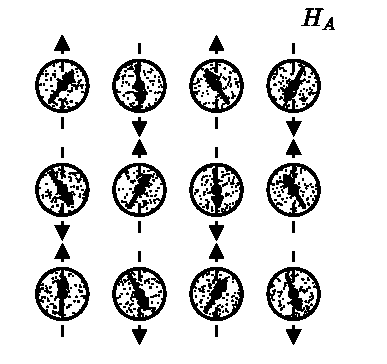
\includegraphics[width=0.72\textwidth]{fig_196.pdf}
\caption*{图 196\quad 反铁磁系统的量子化轴。}
\end{figure}

现在我们相对于对有序“Ising”态的偏离来定义局域的湮没算符与产生算符。在 $\sigma_l$ 为 $+1$ 的格点上，定义与 (10.109) 相同；而在“自旋向下”的格点上，我们要互换 $\mathsf{S}_l^+$ 与 $\mathsf{S}_l^-$ 的角色，因为我们是从第 $l$ 个离子的态 $|{-S}\rangle_l$ 出发来计量的。于是，在每一个格点上——无论“向上”还是“向下”——如下方程
\begin{align*}
\left.
\begin{aligned}
\mathsf{S}_l^x &\approx (\tfrac{1}{2}S)^{\frac{1}{2}}(a_l + a_l^*), \\
\mathsf{S}_l^y &\approx -i\sigma_l (\tfrac{1}{2}S)^{\frac{1}{2}}(a_l - a_l^*), \\
\mathsf{S}_l^z &= \sigma_l (S - a_l^* a_l),
\end{aligned}
\right\} \tag{10.125}
\end{align*}
定义了湮没和产生自旋偏离的算符 $a_l$ 与 $a_l^*$。（在某些论述中，人们在两个不同的子晶格（sublattice）上定义不同的算符；不过由于当 $l \neq l'$ 时 $a_l$ 与 $a_l^*$ 对易，这只是标签的问题。）

把 (10.125) 代入 (10.124) 是相当容易的。第一项就是这个态的“Ising”能量
\begin{equation*}
\mathcal{E}_0 = -\sum_{ll'} J_{ll'}\, \sigma_l \sigma_{l'} S^2 - N\beta S H_A \tag{10.126}
\end{equation*}
这一项我们可以丢弃。其余的项——在 $a_l$、$a_l^*$ 中保留到二阶乘积——虽然复杂，但很容易写出。

仿照 (10.114) 的一个 Fourier 变换引入新的湮没与产生算符 $b_{\mathbf{q}}$ 和 $b_{\mathbf{q}}^*$，使得
\begin{equation*}
a_l = N^{-\frac{1}{2}} \sum_{\mathbf{q}} b_{\mathbf{q}}\, e^{i\mathbf{q}\cdot\mathbf{l}}, \qquad a_l^* = N^{-\frac{1}{2}} \sum_{\mathbf{q}} b_{\mathbf{q}}^*\, e^{-i\mathbf{q}\cdot\mathbf{l}}. \tag{10.127}
\end{equation*}
除了“Ising”能量 (10.126) 之外，我们发现哈密顿量可以写成
\begin{equation*}
\mathcal{H} = \tfrac{1}{2} \sum_{\mathbf{q}} \bigl\{ A_{\mathbf{q}} (b_{\mathbf{q}}^* b_{\mathbf{q}} + b_{-\mathbf{q}}^* b_{-\mathbf{q}}) + B_{\mathbf{q}} (b_{\mathbf{q}} b_{-\mathbf{q}} + b_{\mathbf{q}}^* b_{-\mathbf{q}}^*) \bigr\} + \mathbf{H}\cdot\mathbf{M}, \tag{10.128}
\end{equation*}
其中系数与 (2.12) 或 (10.116) 相类似：——
\begin{align*}
\left.
\begin{aligned}
A_{\mathbf{q}} &= \beta H_A + \sum_{\mathbf{h}} 2S J(\mathbf{h}) \bigl\{ \sigma_{\mathbf{h}} - \tfrac{1}{2}(1 + \sigma_{\mathbf{h}})\cos\mathbf{q}\cdot\mathbf{h} \bigr\}, \\
B_{\mathbf{q}} &= -\sum_{\mathbf{h}} S J(\mathbf{h})(1 - \sigma_{\mathbf{h}})\cos\mathbf{q}\cdot\mathbf{h}.
\end{aligned}
\right\} \tag{10.129}
\end{align*}
在这些表达式中，$\sigma_{\mathbf{h}}$ 表示位于 $\mathbf{h}$ 处的格点相对于中心格点符号的符号。我们可以把 $J(\mathbf{h})$ 的力程比最近邻相互作用更长、甚至在某些距离上为铁磁型的情形也包括进来；唯一必要的条件是 $\sigma_l$ 应当正确地描述 Ising 模型的基态。

在 (10.128) 中，外磁场与一个复杂的算符 $\mathbf{M}$ 联结在一起出现；我们不打算一般地定义它，尽管在简单的情形中可以看出，它对应于一个在两个子晶格的格点上（沿 $z$ 轴）看似正负交替的矩。

这是我们在 (10.125) 中对局域量子化轴的任意选取所造成的结果——对这个项我们就不再深究了。

我们的“交替”态的另一个效应是：(10.128) 中存在把 $b_{\mathbf{q}}$ 与 $b_{-\mathbf{q}}$ 联结起来的项。当我们把 (10.125) 代入 (10.124) 时，它们通过像 $a_l a_{l'}$ 这样的乘积产生，而这类乘积在铁磁态 (10.113) 中并不出现。强加上一个 Ising 自旋背景系统降低了体系的基本平移对称性，因此哈密顿量不再能被 Fourier 变换 (10.127) 自动对角化。或许我们应当取每个晶胞两个自旋，并作一种颇不相同的 Fourier 分析。

然而，这个问题实际上并不比晶格动力学的类似问题中相互作用矩阵 (2.13) 的约化更困难。我们通过一个正则变换引入新变量 $c_{\mathbf{q}}$、$c_{\mathbf{q}}^*$：
\begin{align*}
\left.
\begin{aligned}
b_{\mathbf{q}} &= c_{\mathbf{q}}\cosh\theta_{\mathbf{q}} + c_{-\mathbf{q}}^*\sinh\theta_{\mathbf{q}}, \qquad b_{\mathbf{q}}^* = c_{\mathbf{q}}^*\cosh\theta_{\mathbf{q}} + c_{-\mathbf{q}}\sinh\theta_{\mathbf{q}}, \\
b_{-\mathbf{q}} &= c_{\mathbf{q}}^*\sinh\theta_{\mathbf{q}} + c_{-\mathbf{q}}\cosh\theta_{\mathbf{q}}, \qquad b_{-\mathbf{q}}^* = c_{\mathbf{q}}\sinh\theta_{\mathbf{q}} + c_{-\mathbf{q}}^*\cosh\theta_{\mathbf{q}},
\end{aligned}
\right\} \tag{10.130}
\end{align*}
它保持对易子
\begin{equation*}
[c_{\mathbf{q}}, c_{\mathbf{q}}^*] = \cosh^2\theta_{\mathbf{q}} - \sinh^2\theta_{\mathbf{q}} = 1. \tag{10.131}
\end{equation*}
参数 $\theta_{\mathbf{q}}$ 表示在这四个算符的空间中绕一个虚角度的转动。值得注意的是，$c_{\mathbf{q}}$ 的共轭是 $c_{-\mathbf{q}}^*$；我们必须反转运动方向，才能使它看上去像是给定波的物理共轭。

如果把 (10.130) 代入 (10.128)，就会得到一组“非对角”项
\begin{equation*}
\tfrac{1}{2} \sum_{\mathbf{q}} \bigl\{ 2A_{\mathbf{q}}\cosh\theta_{\mathbf{q}}\sinh\theta_{\mathbf{q}} + B_{\mathbf{q}}(\cosh^2\theta_{\mathbf{q}} + \sinh^2\theta_{\mathbf{q}}) \bigr\} (c_{\mathbf{q}} c_{-\mathbf{q}} + c_{\mathbf{q}}^* c_{-\mathbf{q}}^*), \tag{10.132}
\end{equation*}
只要把 $\theta_{\mathbf{q}}$ 选得满足
\begin{align*}
\frac{B_{\mathbf{q}}}{A_{\mathbf{q}}} &= -\frac{2\cosh\theta_{\mathbf{q}}\sinh\theta_{\mathbf{q}}}{\cosh^2\theta_{\mathbf{q}} + \sinh^2\theta_{\mathbf{q}}} \\
&= -\tanh 2\theta_{\mathbf{q}}, \tag{10.133}
\end{align*}
这组项便可以对每一个 $\mathbf{q}$ 值都变为零。对角项于是给出如下结果
\begin{equation*}
\mathcal{H} = \sum_{\mathbf{q}} \bigl[ (A_{\mathbf{q}}^2 - B_{\mathbf{q}}^2)^{\frac{1}{2}} (c_{\mathbf{q}}^* c_{\mathbf{q}} + \tfrac{1}{2}) - A_{\mathbf{q}} \bigr], \tag{10.134}
\end{equation*}
其中我们已利用对易关系把算符排成了这一顺序。现在的求和遍及 $\mathbf{q}$ 的一切取值，正负兼备。

这个结果与 (10.115) 十分相似。$c_{\mathbf{q}}^* c_{\mathbf{q}}$ 的本征态，比方说记作 $|n_{\mathbf{q}}\rangle$，对应于该模中激发了 $n_{\mathbf{q}}$ 个量子。在简单情形下，反铁磁振子（antiferromagnon）的能量将是
\begin{align*}
\hbar\omega_{\mathbf{q}} &= (A_{\mathbf{q}}^2 - B_{\mathbf{q}}^2)^{\frac{1}{2}} \\
&= \bigl\{ (\beta H_A - 2zSJ)^2 - (2pSJ\langle\cos qa\rangle)^2 \bigr\}^{\frac{1}{2}}, \tag{10.135}
\end{align*}
其中 $\langle\cos qa\rangle$ 是这个量对 $p$ 个最近邻取的平均值，这些近邻与原点相距 $a$，我们假定它们通过交换积分 $J$ 相互作用。如果写成
\begin{equation*}
\hbar\omega_A = \beta H_A, \quad \hbar\omega_J = -2pSJ \tag{10.136}
\end{equation*}
（记得 $J$ 在反铁磁性中是负的），则
\begin{equation*}
\omega_{\mathbf{q}} = \bigl\{ (\omega_A + \omega_J)^2 - (\omega_J\langle\cos qa\rangle)^2 \bigr\}^{\frac{1}{2}} \tag{10.137}
\end{equation*}
就是自旋波谱。

这看上去相当简单。例如，设 $\omega_A \ll \omega_J$，那么
\begin{align*}
\omega_{\mathbf{q}} &\approx \omega_J\bigl\{ 1 - \langle\cos qa\rangle^2 \bigr\}^{\frac{1}{2}} \\
&\approx \frac{1}{\sqrt{3}}\,\omega_J\, .\, qa, \tag{10.138}
\end{align*}
对应于频率对波数呈线性依赖，正如晶格谱 (2.21) 中那样。磁振子对比热的贡献应当按 $T^3$ 变化，也正如 (2.57) 中那样。

让我们试着遵循 (10.122)，计算每个子晶格（sublattice）的磁化强度随温度的变化。平均自旋偏离显然是
\begin{align*}
\langle a_l^* a_l\rangle &= \frac{1}{N}\sum_{\mathbf{q}} \langle b_{\mathbf{q}}^* b_{\mathbf{q}}\rangle \\
&= \frac{1}{N}\sum_{\mathbf{q}} \bigl\langle \cosh^2\theta_{\mathbf{q}}\, c_{\mathbf{q}}^* c_{\mathbf{q}} + \sinh^2\theta_{\mathbf{q}}\, c_{\mathbf{q}} c_{\mathbf{q}}^* \bigr\rangle \\
&= \frac{1}{N}\sum_{\mathbf{q}} \Bigl\{ \bigl(n_{\mathbf{q}} + \tfrac{1}{2}\bigr)\frac{A_{\mathbf{q}}}{\hbar\omega_{\mathbf{q}}} - \tfrac{1}{2} \Bigr\}, \tag{10.139}
\end{align*}
这里用到了变换 (10.127) 与 (10.130)。在此式中 $n_{\mathbf{q}}$ 是第 $q$ 个模中激发的磁振子数；我们自然要用 Bose–Einstein 分布 (10.120) 把它作为温度的函数计算出来。

但是即使在绝对零度，平均自旋偏离也不会消失。在 (10.139) 中取 $n_{\mathbf{q}} = 0$，我们仍然有
\begin{align*}
\langle a_l^* a_l\rangle_{T=0} &= \frac{1}{2N}\sum_{\mathbf{q}} \left( \frac{A_{\mathbf{q}}}{\hbar\omega_{\mathbf{q}}} - 1 \right) \\
&\approx \frac{1}{2N}\sum_{\mathbf{q}} \Bigl\{ \frac{1}{\bigl(1 - \langle\cos qa\rangle^2\bigr)^{\frac{1}{2}}} - 1 \Bigr\} \tag{10.140}
\end{align*}
（在 (10.138) 所描述的简单情形下）。这个和是可以计算的；它的行为如同积分
\begin{equation*}
\int \frac{1}{q}\,\mathrm{d}\mathbf{q} \tag{10.141}
\end{equation*}
只有当 $\mathrm{d}\mathbf{q}$ 是在二维或三维流形上取值时，它才收敛。于是我们证实：一维反铁磁体即使在 $T = 0$ 时也不具有稳定的有序态。这超出了 (10.96) 的结果——后者表明一维 Ising 模型对热涨落是不稳定的；在反铁磁情形，与自旋交换相联系的涨落会摧毁体系所假想的有序基态。

\begin{figure}[H]
\centering
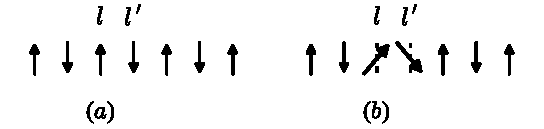
\includegraphics[width=0.72\textwidth]{fig_197.pdf}
\caption*{图 197\quad 在反铁磁有序态 (a) 中，交换算符 $\mathsf{S}_l^+ \mathsf{S}_{l'}^-$ 产生两个自旋偏离 (b)。}
\end{figure}

即使在二维和三维情形，每个子晶格的磁矩也达不到其假定的极大值。事实上，由 (10.125) 中的 $\sigma_l$ 所定义的“交替”态并非真正是哈密顿量的本征态。我们可以试着用 (10.106) 的方法来核查这一点；正如在那里指出的，$\mathsf{S}_l^+ \mathsf{S}_{l'}^-$ 项倾向于把一个自旋偏离从一个格点传递到相邻的下一个格点。而在反铁磁情形，它会在两个相邻格点上同时产生自旋偏离——于是基态必定包含由这种组态及类似组态出发所能得到的一切状态的混合。

三维体系的反铁磁基态并非完全有序（当 $S = \tfrac{1}{2}$ 时，每个子晶格大概只能达到其极大磁矩的 90\%），这一事实也反映在能量的期望值上。从 (10.126)、(10.129) 与 (10.134) 可以看到，它是
\begin{align*}
\langle\mathcal{H}\rangle + \mathcal{E}_0 &= \sum_{\mathbf{q}} \bigl( n_{\mathbf{q}} + \tfrac{1}{2} \bigr) \hbar\omega_{\mathbf{q}} - A_{\mathbf{q}} + \mathcal{E}_0 \\
&= -2NpS(S+1)J + \sum_{\mathbf{q}} \bigl( n_{\mathbf{q}} + \tfrac{1}{2} \bigr) \hbar\omega_{\mathbf{q}}, \tag{10.142}
\end{align*}
即便在 $T = 0$、$n_{\mathbf{q}} = 0$ 时，它也大于人们对“Ising”态算出的对角值。磁振子各模中的“零点能”必须包括进去；它使基态的能量升高，基态能量位于 $-2NpJS(S+1)$ 与 $-2NpJS^2$ 之间的某处。

\begin{figure}[H]
\centering
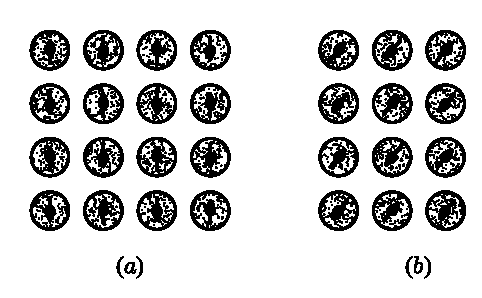
\includegraphics[width=0.72\textwidth]{fig_198.pdf}
\caption*{图 198\quad 在没有各向异性场时，反铁磁阵列 (a) 的自旋可以在能量不变的情况下转动 (b)。}
\end{figure}

关于 (10.139) 还有进一步的一点值得注意。按照 (10.138)，$\omega_{\mathbf{q}}$ 在 $q = 0$ 处为零，这样，在平均自旋偏离的计算中这一项的贡献就会是无穷大。我们需要各向异性场（anisotropy field）$H_A$ 来使得
\begin{equation*}
\omega_{\mathbf{q}} \to \sqrt{\bigl( 2\omega_A\omega_J \bigr)} \quad \text{当}\; q \to 0 \tag{10.143}
\end{equation*}
从而避免这个奇点。事实是：我们的体系在其总自旋为零的基态下，对于如图 198 所示的所有自旋的整体均匀转动是不稳定的。各向异性场正是用来稳定量子化方向的。这个场可以非常小——没有 $H_A$，(10.141) 中的极限在 $q = 0$ 处也可以是有限的——但原则上各向异性场必须存在，而且实际上它也确实存在。

实际上，我们可以把频率 (10.143) 作为体系的反铁磁共振（antiferromagnetic resonance）频率观测到。即使 $H_A$ 只有几百高斯，这也是一个很高的频率，但它可以通过施加一个强的外磁场而被带入共振。

反铁磁有序态的磁化率规则不难核查；当然，关于磁振子–声子相互作用等等也已有各种计算。然而，最有意思的一点或许是：如果我们用 (10.139) 去计算有限温度下子晶格的极化，就会发现一个行为如下的表达式
\begin{align*}
\sum_{\mathbf{q}} \frac{\bar{n}_{\mathbf{q}} A_{\mathbf{q}}}{\hbar\omega_{\mathbf{q}}} &\approx \sum_{\mathbf{q}} \frac{kTA_{\mathbf{q}}}{(\hbar\omega_{\mathbf{q}})^2} \\
&\propto \int \frac{1}{q^2}\,\mathrm{d}\mathbf{q} \tag{10.144}
\end{align*}
它在二维情形下于 $q = 0$ 处对数发散。

这样，交换效应在受到热激发时，就足以摧毁二维 Ising 模型的有序反铁磁态；Onsager 结果在这个情形下对真实自旋并不成立（尽管它对铁磁性确实成立）。积分 (10.144) 在三维情形确实收敛，因此反铁磁态在三维下很可能是稳定的——总会有一个由 (10.35) 那样的偶极–偶极项产生的微小各向异性场。但这一点尚未得到严格证明；其正确性的最好明证，也许当属 §2.6 中提到过的中子衍射实验——它们在物理上直接显示出了两个磁子晶格。

 % 本文件由 scripts/assemble.py 自动装配，勿手改（改 parts/ 后重跑）
% 第11章 超导电性

% 第11章 SUPERCONDUCTIVITY
% 页码核对说明：经与扫描页核对，第 11 章实际始于书页 379（p393.png）；
% p389–p392（书页 375–378）为第 10 章 §10.12 的结尾，归第 10 章文件。
% 本文件实际覆盖书页 379–385（p393–p399）：章首 + §11.1 + §11.2。

\chapter{超导电性}

\epigraphbook{既然变化本是自然的法则，\\ 唯独恒常反而显得奇怪。}{EARL OF ROCHESTER}

\section{电子间的吸引}

超导电性（superconductivity）长期以来被看作金属诸性质中最异乎寻常、最神秘的一种；但是 Bardeen、Cooper 与 Schrieffer 的理论——即\emph{BCS 理论}——已经解释了如此之多，以致我们可以说，如今我们对超导态的理解，几乎不亚于对“正常”态的理解。我们并不打算在这里论及这个庞大而进展迅速的领域的全部内容；重点将放在那些原子过程上，许多不寻常的宏观现象正是由它们引发的。

\begin{figure}[H]
\centering
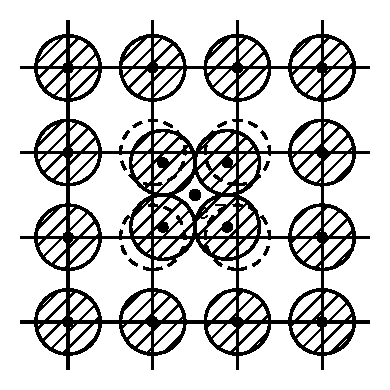
\includegraphics[width=0.72\textwidth]{fig_199.pdf}
\caption*{图 199\quad 电子附近晶格的极化。}
\end{figure}

整个效应源自任意两个能量几乎相同的电子之间的一种微弱吸引力。我们通常认为自由电子通过其库仑相互作用而相互\emph{排斥}；不过，正如 §5.8 所示，在长距离上这个场会因“其他”电子的屏蔽（screening）效应而显著减弱。但在晶格中，电子倾向于把正离子拉向自己，从而被一个晶格比平常略为密集的区域所包围。进入其邻近区域的另一个电子将被引向这个区域；看上去就好像它被第一个电子吸引着。打个比方：两个粒子紧挨着一同坐进床垫的同一个凹坑里，是能够占到便宜的。

计算这种力，最简单的办法是把它描述为一个电子发射“虚”声子、另一个电子吸收此声子的过程。考察图 200(a) 所定义的过程：处于状态 $\mathbf{k}$ 的电子发射一个声子，被散射到状态 $\mathbf{k}-\mathbf{K}$；处于状态 $\mathbf{k}'$ 的电子吸收这个声子，被散射到 $\mathbf{k}'+\mathbf{K}$。

\begin{figure}[H]
\centering
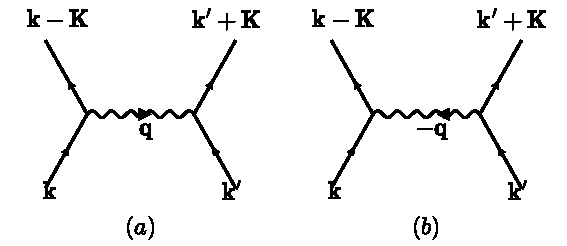
\includegraphics[width=0.72\textwidth]{fig_200.pdf}
\caption*{图 200\quad 通过声子交换的电子–电子相互作用。}
\end{figure}

在二级微扰论中，我们应当用矩阵元
\begin{equation*}
\langle \mathbf{k}-\mathbf{K},\,\mathbf{k}'+\mathbf{K}\,|\,V\,|\,\mathbf{k},\,\mathbf{k}'\rangle
=\frac{\mathcal{M}_{\mathbf{k},\,\mathbf{k}-\mathbf{K}}\,\mathcal{M}^{*}_{\mathbf{k}',\,\mathbf{k}'+\mathbf{K}}}{\mathcal{E}(\mathbf{k})-\mathcal{E}(\mathbf{k}-\mathbf{K})-\hbar\nu_{\mathbf{q}}}.
\tag{11.1}
\end{equation*}
来表示这一跃迁。在这个表达式中，$\mathcal{M}_{\mathbf{k},\mathbf{k}-\mathbf{K}}$ 代表电子–声子相互作用的矩阵元，与 §6.13 中的相同。能量分母代表由初态到中间态的能量变化，其中包括所产生的声子的能量 $\hbar\nu_{\mathbf{q}}$；对 N 过程有 $\mathbf{q}=\mathbf{K}$，不过电子–声子 U 过程也可以包括在内。

还有另一个过程对总散射作出贡献，如图 200(b) 所示：波矢为 $-\mathbf{q}$ 的声子先由 $\mathbf{k}'$ 发射出来，然后被 $\mathbf{k}$ 吸收。它给出一个与式 (11.1) 类似的表达式，只是分母稍有不同。把这两个过程合并起来，并假定电子–声子矩阵元实质上相同，我们就得到
\begin{equation*}
\langle \mathbf{k}-\mathbf{K},\,\mathbf{k}'+\mathbf{K}\,|\,V\,|\,\mathbf{k},\,\mathbf{k}'\rangle
=\frac{|\mathcal{M}_{\mathbf{k},\,\mathbf{k}-\mathbf{K}}|^{2}\,2\hbar\nu_{\mathbf{q}}}{\{\mathcal{E}(\mathbf{k})-\mathcal{E}(\mathbf{k}-\mathbf{K})\}^{2}-(\hbar\nu_{\mathbf{q}})^{2}}.
\tag{11.2}
\end{equation*}
它对电子所产生的效果，就好像两者之间存在一种直接的相互作用，其 Fourier 系数 $V(\mathbf{K})$ 由式 (11.2) 给出。它通常是正的；但对于
\begin{equation*}
|\mathcal{E}(\mathbf{k})-\mathcal{E}(\mathbf{k}-\mathbf{K})|<\hbar\nu_{\mathbf{q}}
\tag{11.3}
\end{equation*}
这一狭窄的能量范围，相互作用是负的，相应于一种吸引力。在式 (11.3) 的范围内，这个力具有 Fourier 分量
\begin{equation*}
V(\mathbf{K})\approx-\frac{2\,|\mathcal{M}_{\mathbf{k},\,\mathbf{k}-\mathbf{K}}|^{2}}{\hbar\nu_{\mathbf{q}}}.
\tag{11.4}
\end{equation*}
这或许算不上一种很强的力。我们是在极低的温度下工作，因此可以把声子发射过程看作由晶格的零点运动所诱发。利用式 (2.109)、(6.86) 与 (6.93)，我们得到
\begin{align*}
|\mathcal{M}_{\mathbf{k},\,\mathbf{k}-\mathbf{K}}|^{2}
&=|\mathcal{U}(\mathbf{K})|^{2}\,|\mathbf{K}\cdot\mathbf{U}_{\mathbf{q}}|^{2}\\
&=|\mathcal{U}(\mathbf{K})|^{2}\,\frac{\mathbf{K}^{2}\hbar}{2NM\nu_{q}},
\tag{11.5}
\end{align*}
式中 $\mathcal{U}(\mathbf{K})$ 是单个离子的屏蔽势的 Fourier 变换。如果只有 N 过程，并且声速由式 (6.84) 正确给出，那么
\begin{align*}
V(\mathbf{K}) &\approx-\frac{|\mathcal{U}(\mathbf{K})|^{2}\,\mathbf{q}^{2}}{NM\nu_{q}^{2}}\\
&=-\frac{|\mathcal{U}(\mathbf{K})|^{2}}{D_{0}s^{2}}=-\frac{3}{2}\,\frac{|\mathcal{U}(\mathbf{K})|^{2}}{NZ\mathcal{E}_{F}}.
\tag{11.6}
\end{align*}
这样，在 N 过程所允许的 $\mathbf{K}$ 值范围内，有效相互作用并不迅速减小。对更大的 $K$ 值，U 过程会使 $V(\mathbf{K})$ 有所增大，不过，正如 §6.13 和 §7.5 中所讨论的，电子 Bloch 态中平面波的混合避免了 $\mathbf{K}=\mathbf{g}$ 处的灾难。显然，这种吸引是短程的——直到两电子之间所能交换动量的最大值，它都具有很大的矩阵元。

当然，电子之间还存在着普通的库仑排斥。如同式 (5.32) 那样，相应的矩阵元应为
\begin{equation*}
V_{\mathrm{Coul.}}(\mathbf{K})=\frac{4\pi e^{2}}{K^{2}+\lambda^{2}},
\tag{11.7}
\end{equation*}
式中 $\lambda$ 是式 (5.22) 的屏蔽参量，或者是像式 (5.36) 那样的某种更复杂的表达式。我们把式 (11.4) 与式 (11.7) 之和取作对 \emph{Fröhlich 相互作用}（Fröhlich interaction）的估计。超导电性的判据就是它应为负值。用电子–声子相互作用来表述，这个判据并没有任何很简单的形式；不过有证据表明，Bardeen 公式 (6.93) 中“赝势部分”$\mathcal{V}'(K)$ 的强度才是关键因素。

上面的论证已经足够简单；但要想恰当地为它辩护，就需要考察电子–声子联合系统的能量中的各种贡献，其中包括 §6.11 中声速的重整化。应当注意，我们处理的只是像式 (11.3) 中那样处于很窄相对能量范围内的电子；在这个范围之外，晶格的运动太慢，跟不上电子的运动。但由于对净相互作用最重要的贡献来自相当大的 $K$ 值——相应于大的 $q$ 值——这个范围的量级为 $k\Theta$，这里 $\Theta$ 是 Debye 温度。既然超导电性只在极低温度下出现，这个能量范围就远比费米面（Fermi surface）上“热层”的厚度 $kT$ 宽广得多。因此，对于那些真正能够参与超导转变的电子来说，近似式 (11.4) 是合理的。

\section{Cooper 对}

为了领会电子之间交换声子所产生的吸引力的效果，我们现在来计算总散射振幅 $t$，即这样一个矩阵元：它的平方给出下述过程的概率——处于 $\mathbf{k}_1$ 和 $\mathbf{k}_2$ 两态的两个电子被散射到另外两个态 $\mathbf{k}_1'$ 和 $\mathbf{k}_2'$。如图 201(a) 那样，我们将假定这些态正好位于费米球（Fermi sphere）之外。

对散射最显而易见的贡献将是式 (11.2) 所定义的直接相互作用 $V(\mathbf{K})$。它对我们眼下的计算来说未免太复杂，所以让我们抽出其中的吸引部分，并假定它是一个常数。于是，我们的一级散射振幅将取为
\begin{equation*}
t_{1}=V(\mathbf{K})=V,
\tag{11.8}
\end{equation*}
其中 $V$ 是一个负的常数，与 $\mathbf{k}_1'$ 和 $\mathbf{k}_1$ 无关。但这个吸引势只对能量几乎相同的电子才成立；为了把条件 (11.3) 纳入理论，我们将约定：除非
\begin{equation*}
|\mathcal{E}(\mathbf{k}_{1})-\mathcal{E}(\mathbf{k}_{2})|<w,
\tag{11.9}
\end{equation*}
否则 $V(\mathbf{K})$ 为零，这里 $w$ 是一个常数。由式 (11.3) 显然可见，$w$ 应当具有 $k\Theta$ 的量级。

通常在散射问题中，近似式 (11.8) 已经足够。然而，在 $t$ 的微扰展开中还会有一些进一步的项，对应于电子从 $\mathbf{k}_1$ 出发、终于 $\mathbf{k}_1'$ 的逐次虚过程。例如，下一项可能就是图 201(b) 所示的过程：我们在初态与终态之间插入一个虚态，其中 $\mathbf{k}_1$ 先变到 $\mathbf{k}_1+\mathbf{K}$、$\mathbf{k}_2$ 先变到 $\mathbf{k}_2-\mathbf{K}$，然后再作第二次跃迁，变到 $\mathbf{k}_1'$ 和 $\mathbf{k}_2'$。

\begin{figure}[H]
\centering
\includegraphics[width=0.72\textwidth]{fig_201.pdf}
\caption*{图 201\quad (a) 电子的直接散射。(b) 二阶项。}
\end{figure}

这种过程对散射振幅的贡献由通常的微扰表达式给出：
\begin{equation*}
t_{2}(\mathbf{K})=\frac{V^{2}}{\mathcal{E}(\mathbf{k}_{1})+\mathcal{E}(\mathbf{k}_{2})-\mathcal{E}(\mathbf{k}_{1}+\mathbf{K})-\mathcal{E}(\mathbf{k}_{2}-\mathbf{K})}.
\tag{11.10}
\end{equation*}
但这一项只在非常有限的条件下才存在。由于 Pauli 原理，中间态不得位于费米面以下；而且按式 (11.9)，每次跃迁的能量差必须小于 $w$。于是我们得到如下规则：
\begin{equation*}
\mathcal{E}_{F}<\mathcal{E}(\mathbf{k}_{1}+\mathbf{K})<\mathcal{E}(\mathbf{k}_{1})+w,\quad
\mathcal{E}_{F}<\mathcal{E}(\mathbf{k}_{2}-\mathbf{K})<\mathcal{E}(\mathbf{k}_{2})+w,
\tag{11.11}
\end{equation*}
等等；如果式 (11.10) 还想对 $t_2$ 有任何贡献的话，这些规则就必须得到满足。这些条件类似于 Kondo 效应（§10.6）中虚自旋翻转跃迁的选择定则；在同时计及直接过程和交换过程时，各个态的占据数并\emph{不}会从二阶项中消去。

这些规则限制性如此之强，以致通常我们可以忽略 $t_2$。但当 $\mathbf{k}_1$ 和 $\mathbf{k}_2$ 的方向近乎相反时，条件 (11.11) 的两式合二为一，对可能发生散射的 $\mathbf{K}$ 值范围也就不再施加那么苛刻的限制。事实上，此时 $t_2$ 可以变得相当大。

为说明这一点，方便的做法是从费米能级（Fermi level）起量度能量。我们对每个态定义
\begin{align*}
\xi(\mathbf{k}) &\equiv \mathcal{E}(\mathbf{k})-\mathcal{E}_{F}\\
&\approx \hbar v_{F}(k-k_{F})
\tag{11.12}
\end{align*}
（只要 $k$ 近似等于 $k_F$）。我们还引入两个具有能量量纲的新辅助变量
\begin{equation*}
\Delta=\xi(\mathbf{k}_{1})+\xi(\mathbf{k}_{2}),\qquad
\eta=\hbar v_{F}\,|\mathbf{k}_{1}+\mathbf{k}_{2}|
\tag{11.13}
\end{equation*}
它们量度的是我们这对电子的总能量和总动量。

为得到二阶微扰项，我们把式 (11.10) 在满足式 (11.11) 的所有 $\mathbf{K}$ 值上积分。利用式 (11.12) 和 (11.13)，这可以化成一个更简单的公式：
\begin{align*}
t_{2} &= V^{2}\int \frac{\mathrm{d}\mathbf{K}}{\mathcal{E}(\mathbf{k}_{1})+\mathcal{E}(\mathbf{k}_{2})-\mathcal{E}(\mathbf{k}_{1}+\mathbf{K})-\mathcal{E}(\mathbf{k}_{2}-\mathbf{K})}\\
&= \frac{2\pi V^{2}k_{F}^{2}}{8\pi^{3}\hbar v_{F}}\int_{0}^{w}\mathrm{d}\xi\int_{-1}^{1}\frac{\mathrm{d}(\cos\theta)}{\Delta+\eta\cos\theta-2\xi}.
\tag{11.14}
\end{align*}

\begin{figure}[H]
\centering
\includegraphics[width=0.72\textwidth]{fig_202.pdf}
\caption*{图 202\quad (a) 在 $\mathbf{k}_3$ 处产生一个空穴、随后又被 $\mathbf{k}_2$ 填充的过程。(b) 逐次的对散射。(c) 涉及空穴的对散射。}
\end{figure}

当 $\Delta$ 和 $\eta$ 都远小于 $w$ 时，被积函数中出现一个奇点，它使积分呈对数行为（可参照式 (10.56)）：
\begin{equation*}
t_{2}\approx-\frac{V^{2}}{4\pi^{2}}\,\frac{k_{F}^{2}}{\hbar v_{F}}\ln\frac{2w}{\max{(\Delta,\eta)}}.
\tag{11.15}
\end{equation*}
通常这一项远小于 $t_1$，原本可以忽略。但如果 $\Delta$ 和 $\eta$ 恰好都非常小，式 (11.15) 就可能变得很大——这时我们或许不得不考虑 $t$ 的微扰级数中更进一步的项。

这样的项可能非常复杂，因为我们可以考虑如图 202(a) 那样的虚过程：一个来自费米面内部的电子与这对电子中的一个发生相互作用，留下一个空穴，而这个空穴最终在此后的某个过程中被填满。不过，这类过程在微扰级数中给出的贡献往往小得多。重要的是那些把图 201(b) 所示过程一再重复的情形——电子对不断地自我散射，如图 202(b) 那样。每一次这样的虚散射都引入一个类似于式 (11.15) 的因子，当 $\Delta$ 和 $\eta$ 很小时还包括那个大的对数积分。

为了得到正确的结果，我们还必须把这样的过程包括进来：一对电子从费米海（Fermi sea）中被散射出去，留下一对空穴，它们可以接收 $\mathbf{k}_1$ 和 $\mathbf{k}_2$ 处的电子（图 202(c)）。这一过程对 $t_2$ 给出与式 (11.15) 相同的贡献。把所有这些项加起来，我们看到散射振幅必定表现为无穷级数
\begin{equation*}
t\approx V+\gamma V^{2}+\gamma^{2}V^{3}+\ldots,
\tag{11.16}
\end{equation*}
其中
\begin{equation*}
\gamma=-\frac{1}{2\pi^{2}}\,\frac{k_{F}^{2}}{\hbar v_{F}}\ln\frac{2w}{\max{(\Delta,\eta)}}.
\tag{11.17}
\end{equation*}
但级数 (11.16) 可以求和：
\begin{equation*}
t\approx\frac{V}{1-\gamma V}.
\tag{11.18}
\end{equation*}
这样，散射振幅的行为就好像它含有一个极点。这是众所周知的一个征兆，表明自由粒子彼此散射的假设已经失效；它正是两个电子形成\emph{束缚态}（bound state）的标志。假设我们取 $\eta=0$，使得 $\mathbf{k}_1=-\mathbf{k}_2$。极点出现时的能量由下式确定：
\begin{align*}
1&=\gamma V\\
&=-\frac{V}{2\pi^{2}}\,\frac{k_{F}^{2}}{\hbar v_{F}}\ln\frac{2w}{\Delta}.
\tag{11.19}
\end{align*}
（译注：原书式 (11.19) 第二行分母印作 $v_F$，漏排 $\hbar$；由式 (11.17) 显见应有 $\hbar v_F$，译文已补正。）

换句话说，当这对电子的总能量在费米能级以下等于
\begin{equation*}
\Delta_{0}=2w\exp\left(-\frac{2\pi^{2}\hbar v_{F}}{|V|\,k_{F}^{2}}\right)
\tag{11.20}
\end{equation*}
时，它们就倾向于彼此束缚而形成一个“准分子”（quasi-molecule）。这样的状态称为 \emph{Cooper 对}（Cooper pair）。

这类态有可能存在，但这并没有解决超导电性的问题。我们可以这样论证：金属中所有的电子都倾向于结成这样的对——$\mathbf{k}$ 与 $-\mathbf{k}$ 相配，而且这种由 Bose–Einstein 型“准分子”组成的气体随后便能发生 Bose–Einstein 凝聚。然而这些电子对并不稳定；作为对超导态的描述，这种说法有启发性，却缺乏说服力。

最重要的结果是关于电子对能量的公式 (11.20)。我们可以采用自由电子模型，它给出
\begin{align*}
\frac{k_{F}^{2}}{2\pi^{2}\hbar v_{F}} &= \frac{1}{2}\,\mathcal{N}(\mathcal{E}_{F})\\
&= \frac{3}{4}\,\frac{ZN}{\mathcal{E}_{F}}
\tag{11.21}
\end{align*}
（在 BCS 理论中，这个量记作 $N(0)$，即费米能级处\emph{每个自旋}的态密度）。把式 (11.6) 代入式 (11.20)，并取 $w\approx k\Theta$，就应当得到
\begin{align*}
\Delta_{0} &\approx 2k\Theta\exp\{-2/\mathcal{N}(\mathcal{E}_{F})\,|V|\}\\
&\approx 2k\Theta\exp\{-8\mathcal{E}_{F}^{2}/9\,|\mathcal{U}|^{2}\}.
\tag{11.22}
\end{align*}
如果我们假定 $\Delta_{0}$ 是超导转变能量的某种量度，并令它等于 $kT_{c}$，就会发现转变温度 $T_{c}$ 应当介于 Debye 温度的 1/10 与 1/10,000 之间，视电子–离子相互作用势 $|\mathcal{U}|$ 的大小而定。实际观察到的正是如此——我们现在可以理解，为什么 $T_{c}$ 与 $\Theta$ 相差得如此悬殊。

由这个论证还可得出的另一个效应是\emph{同位素效应}（isotope effect）。如果考虑改变每个离子的质量 $M$ 而不改变原子间的作用力，那么我们预期声速按 $M^{-1/2}$ 变化。于是我们预期 $\Theta$ 也按同样的方式变化，从而
\begin{equation*}
T_{c}\propto M^{-1/2},
\tag{11.23}
\end{equation*}
这在许多情形中与观察结果大体相符。

关于 Cooper 对还有一点：如果两个电子除动量相反之外自旋也相反，它们将束缚得更牢。这一点从我们刚才给出的论证看并不明显，而是在计算吸引势 (11.2) 时显露出来的。§11.1 的论证假定我们处理的是可分辨粒子，即自旋相反的电子。倘若两个电子自旋相同，我们就必须援引 Pauli 原理，在计算有效相互作用时使用反对称化的波函数。“交换”项的计入会削弱吸引力，因为这时我们必须设法阻止两个电子进入同一状态或占据同一位置。Cooper 对的单态就是这个准分子的最低态。

\section{超导基态}

上述结果提示了超导态的两个重要特征：它是一个无法用微扰展开中的有限多项来达到的态，因为函数 (11.20) 在 $V=0$ 附近不是 $V$ 的解析函数；它是一个电子以某种方式配成对的态，$\mathbf{k}$ 与 $-\mathbf{k}$ 相配。这个态的构造最初是由 Bardeen、Cooper 和 Schrieffer 所完成的。为了演示他们的解，我们将采用 Bogoliubov 的方法。

完全可以避开有关波函数的一切讨论，而把整个问题用算符语言表述出来，这是非常方便的。我们需要表述这样一个事实：我们有 $N$ 个电子，其能量主要是动能，处在由矢量 $\mathbf{k}$ 和自旋指标 $\sigma$ 标记的态上，并且它们通过势 $V(\mathbf{K})$ 发生相互作用。我们定义湮没算符和产生算符 $b_{\mathbf{k}\sigma}$、$b^{*}_{\mathbf{k}\sigma}$，它们类似于式 (2.129) 和 (10.109) 中定义的算符 $a_{\mathbf{q}}$、$a^{*}_{\mathbf{q}}$，只不过我们现在处理的是费米子。这意味着它们必须服从\emph{反对易关系}（anticommutation relations）
\begin{align*}
[b_{\mathbf{k}\sigma},\,b^{*}_{\mathbf{k}'\sigma'}]_{+} &\equiv b_{\mathbf{k}\sigma}b^{*}_{\mathbf{k}'\sigma'}+b^{*}_{\mathbf{k}'\sigma'}b_{\mathbf{k}\sigma}\\
&=\delta_{\mathbf{k}\mathbf{k}'}\,\delta_{\sigma\sigma'}.
\tag{11.24}
\end{align*}
这个定义的结果是，算符
\begin{equation*}
n_{\mathbf{k}\sigma}=b^{*}_{\mathbf{k}\sigma}b_{\mathbf{k}\sigma}
\tag{11.25}
\end{equation*}
量度态 $(\mathbf{k},\sigma)$ 的占据数，并且如 Pauli 原理所要求的那样，本征值取 0 和 1。当式 (11.24) 中的 $\mathbf{k}$ 与 $\mathbf{k}'$、或 $\sigma$ 与 $\sigma'$ 不相同时，反对易子体现的是反对称原理：交换两个态的标记将使波函数反号。

我们这个系统的 Hamilton 量可以写成
\begin{equation*}
\mathcal{H}=\sum_{\mathbf{k}\sigma}\xi(\mathbf{k})\,b^{*}_{\mathbf{k}\sigma}b_{\mathbf{k}\sigma}+\sum_{\mathbf{k}_1,\,\mathbf{k}_2,\,\mathbf{K}}V(\mathbf{K})\,b^{*}_{\mathbf{k}_2-\mathbf{K},\downarrow}\,b^{*}_{\mathbf{k}_1+\mathbf{K},\uparrow}\,b_{\mathbf{k}_1,\uparrow}\,b_{\mathbf{k}_2,\downarrow}.
\tag{11.26}
\end{equation*}
第一项代表电子的动能，像式 (11.12) 中那样，从费米能级算起。为了方便，常常假定这个能量可以变动——即电子总数 $n$ 并非严格固定——办法是引进电子气的化学势 $\zeta$，并把第一项写成
\begin{align*}
\mathcal{H}_{0}&=\sum_{\mathbf{k}\sigma}n_{\mathbf{k}\sigma}\,\xi(\mathbf{k})\\
&=\sum_{\mathbf{k}\sigma}n_{\mathbf{k}\sigma}\{\mathcal{E}(\mathbf{k})-\zeta\}\\
&=\sum_{\mathbf{k}\sigma}n_{\mathbf{k}\sigma}\,\mathcal{E}(\mathbf{k})-n\zeta.
\tag{11.27}
\end{align*}
式 (11.26) 中的第二项代表由相互作用 (11.2) 所定义的散射，其效果是把 $\mathbf{k}_1$ 和 $\mathbf{k}_2$ 中的电子“湮没”掉，然后再把它们“重新产生”在 $\mathbf{k}_1+\mathbf{K}$ 和 $\mathbf{k}_2-\mathbf{K}$ 处，矩阵元为 $V(\mathbf{K})$。这里我们假定只有自旋相反的电子之间才有相互作用。

Bogoliubov 方法是对算符集 $b_{\mathbf{k}\sigma}$ 与 $b^{*}_{\mathbf{k}\sigma}$ 作一个正则变换，把它们变成具有同样对易关系的一套新的湮没算符和产生算符。特别地，这些新算符必须显示出某种配对性质——正如 Cooper 效应所提示的，它们必须把态 $(\mathbf{k},\uparrow)$ 与态 $(-\mathbf{k},\downarrow)$ 联结起来。

为简单起见，让我们略去自旋指标，写成
\begin{equation*}
\left.\begin{array}{ll}
\beta^{*}_{\mathbf{k}}=u_{\mathbf{k}}b^{*}_{\mathbf{k}}-v_{\mathbf{k}}b_{-\mathbf{k}}, &\quad \beta_{\mathbf{k}}=u_{\mathbf{k}}b_{\mathbf{k}}-v_{\mathbf{k}}b^{*}_{-\mathbf{k}},\\
\beta^{*}_{-\mathbf{k}}=u_{\mathbf{k}}b^{*}_{-\mathbf{k}}+v_{\mathbf{k}}b_{\mathbf{k}}, &\quad \beta_{-\mathbf{k}}=u_{\mathbf{k}}b_{-\mathbf{k}}+v_{\mathbf{k}}b^{*}_{\mathbf{k}}.
\end{array}\right\}
\tag{11.28}
\end{equation*}
（译注：原书 (11.28) 第一式排印为“$\beta_{\mathbf{k}}\ \ u_{\mathbf{k}}b^{*}_{\mathbf{k}}-v_{\mathbf{k}}b_{-\mathbf{k}}$”，漏印等号与 $\beta$ 上的星号；按变换关系此处应为第二式的 Hermite 共轭，译文已补正。）

如果
\begin{equation*}
u^{2}_{\mathbf{k}}+v^{2}_{\mathbf{k}}=1
\tag{11.29}
\end{equation*}
则算符 $\beta_{\mathbf{k}}$、$\beta^{*}_{\mathbf{k}}$ 就会具有费米子应有的反对易关系。
这个变换确实与反铁磁自旋波的变换 (10.130) 本质上相同，只不过现在我们是在 $\mathbf{k}$ 与 $-\mathbf{k}$ 的空间中作一个“真实转动”，于是
\begin{equation*}
u_{\mathbf{k}}=\cos\theta_{\mathbf{k}},\quad v_{\mathbf{k}}=\sin\theta_{\mathbf{k}}
\tag{11.30}
\end{equation*}
满足式 (11.29)。这是因为我们现在处理的是费米子，而不是玻色子。

当我们从式 (11.28) 解出原来的算符并代入 Hamilton 量 (11.26) 时，会得到形形色色的项，其中含有新算符 $\beta_{\mathbf{k}}$、$\beta^{*}_{\mathbf{k}}$ 的乘积。现在，只要某一项中含有湮没算符 $b_{\mathbf{k}}$，我们就可以利用反对易子把它移到右边，例如
\begin{equation*}
\beta_{\mathbf{k}}\beta^{*}_{\mathbf{k}'}=\delta_{\mathbf{k}\mathbf{k}'}-\beta^{*}_{\mathbf{k}'}\beta_{\mathbf{k}}.
\tag{11.31}
\end{equation*}
假定我们的超导态就是这些新算符的“真空”$|0\rangle$。按定义，真空中不存在任何能被湮没的对象，因此
\begin{equation*}
\beta_{\mathbf{k}}|0\rangle=0,
\tag{11.32}
\end{equation*}
对所有 $\mathbf{k}$ 成立。Hamilton 量中的这类项对基态 $|0\rangle$ 的能量没有贡献；于是基态是 $\mathcal{H}$ 中这一部分的本征态。

但是还剩下一些项不能用这种方式消去——即只含有像 $\beta^{*}_{\mathbf{k}}$ 这样的产生算符的项。它们来自 (11.26) 的动能部分，也来自相互作用项的约化——例如当式 (11.31) 中的 $\mathbf{k}$ 与 $\mathbf{k}'$ 恰好相等时。我们发现，Hamilton 量可以写成
\begin{align*}
\mathcal{H}&=2\sum_{\mathbf{k}}\xi(\mathbf{k})\,v^{2}_{\mathbf{k}}+\sum_{\mathbf{k},\,\mathbf{K}}V(\mathbf{K})\,u_{\mathbf{k}}v_{\mathbf{k}}u_{\mathbf{k}+\mathbf{K}}v_{\mathbf{k}+\mathbf{K}}\\
&\quad+\sum_{\mathbf{k}}\bigl\{2\xi(\mathbf{k})\,u_{\mathbf{k}}v_{\mathbf{k}}+(u^{2}_{\mathbf{k}}-v^{2}_{\mathbf{k}})\sum_{\mathbf{K}}V(\mathbf{K})\,u_{\mathbf{k}+\mathbf{K}}v_{\mathbf{k}+\mathbf{K}}\bigr\}\beta^{*}_{\mathbf{k}}\beta^{*}_{-\mathbf{k}}.
\tag{11.33}
\end{align*}
前面的这些项将给出我们基态的能量——只要我们能把最后那个求和中的产生算符消去。

这跟我们在 (10.132) 中遇到的情况非常相似——我们采用同样的手法。我们这样选取变换系数 $u_{\mathbf{k}}$、$v_{\mathbf{k}}$，使每个“危险”项都等于零。令
\begin{equation*}
2\xi(\mathbf{k})\,u_{\mathbf{k}}v_{\mathbf{k}}+(u^{2}_{\mathbf{k}}-v^{2}_{\mathbf{k}})\sum_{\mathbf{K}}V(\mathbf{K})\,u_{\mathbf{k}+\mathbf{K}}v_{\mathbf{k}+\mathbf{K}}=0.
\tag{11.34}
\end{equation*}
一般说来，这是关于未知函数 $u_{\mathbf{k}}$ 和 $v_{\mathbf{k}}$ 的一个复杂的积分方程，而且它们还须满足条件 (11.29)。但让我们采用 (11.8) 和 (11.9) 的假定，把吸引势 $V(\mathbf{K})$ 简化为在能量范围 $\pm w$ 之内取常数值 $V$、在此范围之外为零。我们把式 (11.34) 中对 $\mathbf{K}$ 的求和记作一个参量
\begin{equation*}
\Delta_{0}=-V\sum_{-w}^{w}u_{\mathbf{k}+\mathbf{K}}v_{\mathbf{k}+\mathbf{K}},
\tag{11.35}
\end{equation*}
然后联立求解 (11.34) 与 (11.29)。结果是
\begin{equation*}
u^{2}_{\mathbf{k}}=\frac{1}{2}\biggl[1+\frac{\xi(\mathbf{k})}{\sqrt{\{\Delta^{2}_{0}+\xi^{2}(\mathbf{k})\}}}\biggr],\quad v^{2}_{\mathbf{k}}=\frac{1}{2}\biggl[1-\frac{\xi(\mathbf{k})}{\sqrt{\{\Delta^{2}_{0}+\xi^{2}(\mathbf{k})\}}}\biggr],
\tag{11.36}
\end{equation*}
把它代回 (11.35)，便得到
\begin{align*}
1&=-\frac{1}{2}V\sum_{-w}^{w}\{\Delta^{2}_{0}+\xi^{2}(\mathbf{k})\}^{-\frac{1}{2}}\\
&=-\frac{1}{2}\,\mathcal{N}(\mathcal{E}_{F})\,V\ln\frac{2w}{\Delta_{0}},
\tag{11.37}
\end{align*}
这是在费米面附近对 $\xi$ 的范围积分而来的（记住自旋只计一种）。这与 (11.19) 完全相同。参量 $\Delta_{0}$ 恰恰就是一个 Cooper 对的结合能，与 (11.20) 或 (11.22) 中的一样。

我们可以把这个结果代回 (11.33) 的其余部分——现在其中所有的算符都已消去。我们得到
\begin{equation*}
\mathcal{E}_{0}=2\sum_{\xi<0}\xi(\mathbf{k})-\frac{1}{2}\Delta^{2}_{0}\sum_{\mathbf{k}}\{\Delta^{2}_{0}+\xi^{2}(\mathbf{k})\}^{-\frac{1}{2}}.
\tag{11.38}
\end{equation*}
于是，态 $|0\rangle$ 是 $\mathcal{H}$ 的一个本征态——但其能量低于电子填满的费米球，后者的能量本来正好是各被占据态的 $\xi(\mathbf{k})$ 值之和，如 (11.27) 那样。还可以证明，对于电子总数的期望值 $n$ 的变动而言，这个态使能量取极小，正如 (11.27) 所要求的。

\section{准粒子与能隙}

超导态 $|0\rangle$ 的本性是什么？按定义，它是算符 $\beta^{*}_{\mathbf{k}}$、$\beta_{\mathbf{k}}$ 的“真空”。这些算符能够产生和消灭真空的激发，正如原来的算符 $b^{*}_{\mathbf{k}}$ 和 $b_{\mathbf{k}}$ 能够“产生”和“消灭”电子一样。这样一种激发看上去会是什么样子？按照 (11.28)，$\beta^{*}_{\mathbf{k}}$ 的效果是以振幅 $u_{\mathbf{k}}$“产生”一个处在态 $\mathbf{k}$ 中的电子，同时又以振幅 $v_{\mathbf{k}}$“消灭”一个处在态 $-\mathbf{k}$ 中的电子。

这些系数由 (11.36) 给出。假定 $\mathbf{k}$ 远在费米面之上，使得 $\xi(\mathbf{k})\gg\Delta_{0}$，那么 $u^{2}_{\mathbf{k}}\approx 1$，而 $v^{2}_{\mathbf{k}}\approx 0$。我们的激发看上去就会像一个普通的电子。
\begin{figure}[H]
\centering
\includegraphics[width=0.72\textwidth]{fig_203.pdf}
\caption*{图 203\quad 准粒子。}
\end{figure}
但是现在，当我们逼近费米能级时，$\xi(\mathbf{k})$ 趋于零，$b^{*}_{\mathbf{k}}$ 的振幅将减小，而 $b_{-\mathbf{k}}$ 的振幅将增大。当 $\xi(\mathbf{k})$ 为负时，$v^{2}_{\mathbf{k}}$ 的值将大于 $\frac{1}{2}$；当我们远在费米能级之下时，$v^{2}_{\mathbf{k}}\approx 1$ 而 $u^{2}_{\mathbf{k}}\approx 0$。这时我们的激发相应于在 $-\mathbf{k}$ 处一个电子的“毁灭”，也就是说，它是本已被占据的诸态中的一个“空穴”。

因此，超导态的激发是颇为奇特的\emph{准粒子}（quasi-particle），当它们通过费米能级时，会从“电子”变成“空穴”。在 $\Delta_{0}$ 附近的能量范围内，每个准粒子都是 $\mathbf{k}$ 处的一个电子与 $-\mathbf{k}$ 处的一个空穴的混合体。Cooper 对本身不再出现，但是动量相反（当然还有自旋相反）的电子之间的关联是显而易见的。实际上，我们是在坚持：配对态中各波函数的相位之间应当存在一种关系。

激发的能量也可以计算。我们在 (11.26) 的展开式中寻找含下列算符
\begin{equation*}
n'_{\mathbf{k}}=\beta^{*}_{\mathbf{k}}\beta_{\mathbf{k}}
\tag{11.39}
\end{equation*}
的各项的系数，因为它量度的是在此模式中被激发的准粒子的数目。结果是
\begin{align*}
\epsilon(\mathbf{k})&=\xi(\mathbf{k})\,(u^{2}_{\mathbf{k}}-v^{2}_{\mathbf{k}})-2u_{\mathbf{k}}v_{\mathbf{k}}\sum_{\mathbf{K}}V(\mathbf{K})\,u_{\mathbf{k}+\mathbf{K}}v_{\mathbf{k}+\mathbf{K}}\\
&=\sqrt{\{\Delta^{2}_{0}+\xi^{2}(\mathbf{k})\}}
\tag{11.40}
\end{align*}
（对我们的简化相互作用，用了 (11.35) 和 (11.36)）。
\begin{figure}[H]
\centering
\includegraphics[width=0.72\textwidth]{fig_204.pdf}
\caption*{图 204\quad 准粒子的能量。}
\end{figure}
这一点非常重要，因为它证明了在超导基态之上存在\emph{能隙}（energy gap）$\Delta_{0}$。当 $\xi(\mathbf{k})\gg\Delta_{0}$ 时，$\epsilon(\mathbf{k})\approx\xi(\mathbf{k})$——准粒子的能量就是把一个普通电子激发到费米能级之上所需的能量。但当 $\mathbf{k}$ 趋近费米面（那里 $\xi(\mathbf{k})$ 为零）时，准粒子的能量趋于常数值 $\Delta_{0}$。然后，随着 $\mathbf{k}$ 再进一步减小，$\epsilon(\mathbf{k})$ 又重新增大，直至几乎等于 $|\xi(\mathbf{k})|$。这当然就是把一个电子从负能量态 $\xi(\mathbf{k})$ 中移出所需的能量，正如我们根据对准粒子算符的解释所预期的那样。
因此，超导态是一种“凝聚”态，其含义是：要使整个系统产生一个激发态，需要有限的能量 $\Delta_{0}$。在某些方面，它有点像半导体——在半导体中，要想把一个电子送入导带，也必须越过一有限的带隙。这个类比有助于粗略地解释超导体的某些特殊性质，例如电磁吸收（参见 §8.5）和隧穿（§6.8）。

\section{能隙随温度的变化}

基态只适用于 $T=0$ 的情形。在有限温度下，我们预期会有准粒子按通常的 费米–狄拉克 函数被激发：
\begin{equation*}
f_{\mathbf{k}}=\frac{1}{e^{\epsilon(\mathbf{k})/kT}+1}.
\tag{11.41}
\end{equation*}
在正常态中，这类激发无论在费米能级之上还是之下，都彼此独立。在超导态中，它们倾向于相互合作地发生作用，并破坏能隙。

让我们假定所处理的是态 $|f_{\mathbf{k}}\rangle$，其中第 $\mathbf{k}$ 个态中准粒子的平均数目由 (11.41) 给出。湮没算符 $b_{\mathbf{k}}$ 作用在这个态上的效果不再是零。平均而言，我们可以把 (11.25) 换成
\begin{equation*}
b^{*}_{\mathbf{k}}b_{\mathbf{k}}|f_{\mathbf{k}}\rangle=f_{\mathbf{k}}|f_{\mathbf{k}}\rangle.
\tag{11.42}
\end{equation*}
把 Hamilton 量约化成对角形式的做法，当应用于态 $|0\rangle$ 时，依靠的是 (11.32)。如果现在对态 $|f_{\mathbf{k}}\rangle$ 试着做同样的事情，就会多出一些额外的项；它们来自像 (11.31) 那样把算符乘积约化成标准次序的过程，并乘在 (11.33) 中那些“危险”乘积 $\beta^{*}_{\mathbf{k}}\beta^{*}_{-\mathbf{k}}$ 上。为了从 Hamilton 量中去掉这些“产生电子对”的部分，我们的条件 (11.34) 必须改成为
\begin{equation*}
2\xi(\mathbf{k})\,u_{\mathbf{k}}v_{\mathbf{k}}+(u^{2}_{\mathbf{k}}-v^{2}_{\mathbf{k}})\sum_{\mathbf{K}}V(\mathbf{K})\,u_{\mathbf{k}+\mathbf{K}}v_{\mathbf{k}+\mathbf{K}}(1-2f_{\mathbf{k}+\mathbf{K}})=0
\tag{11.43}
\end{equation*}
（这里计及与每个 $\mathbf{k}$ 相联系的两个可能的自旋态）。

对于简化的相互作用 $V$，这个积分方程可以这样求解：把 (11.35) 和 (11.36) 中的 $\Delta_{0}$ 换成
\begin{equation*}
\Delta=-V\sum_{-w}^{w}u_{\mathbf{k}+\mathbf{K}}v_{\mathbf{k}+\mathbf{K}}(1-2f_{\mathbf{k}+\mathbf{K}}).
\tag{11.44}
\end{equation*}
代替 (11.37)，利用 (11.41)，我们便得到
\begin{align*}
1&=-\frac{1}{2}V\sum_{-w}^{w}\frac{1}{\epsilon(\mathbf{k})}\tanh\frac{\epsilon(\mathbf{k})}{2kT}\\
&=-\frac{1}{2}\,\mathcal{N}(\mathcal{E}_{F})\,V\int_{-w}^{w}\frac{1}{\epsilon}\tanh\frac{\epsilon}{2kT}\,d\xi,
\tag{11.45}
\end{align*}
其中 $\epsilon$ 和以前一样，是一个激发的能量，
\begin{equation*}
\epsilon(\mathbf{k})=\sqrt{\{\Delta^{2}+\xi^{2}(\mathbf{k})\}}.
\tag{11.46}
\end{equation*}
式 (11.45) 与式 (11.46) 这两个方程给出 $\Delta$ 与 $T$ 之间的一个隐含关系。这个关系相当杂乱，但要点在于：当 $T$ 增大时，$\Delta$ 从 $T=0$ 处的 $\Delta_{0}$ 逐渐减小。换言之，能隙 $\Delta$ 随温度升高而减小，并在一个完全确定的温度 $T_{c}$ 处闭合为零；由 (11.46)，在该处 $\epsilon(\mathbf{k})=|\xi(\mathbf{k})|$。于是，我们可以通过积分
\begin{equation*}
\frac{2}{\mathcal{N}(\mathcal{E}_{F})\,V}=2\int_{0}^{w}\frac{1}{\epsilon}\tanh\left(\frac{\epsilon}{2kT_{c}}\right)d\epsilon,
\tag{11.47}
\end{equation*}
求出 $T_{c}$，其解为
\begin{equation*}
\Delta_{0}\approx 1.76\,kT_{c},
\tag{11.48}
\end{equation*}
\begin{figure}[H]
\centering
\includegraphics[width=0.72\textwidth]{fig_205.pdf}
\caption*{图 205\quad 能隙随温度的变化。}
\end{figure}
式中的 $\Delta_{0}$ 由 (11.22) 表示，即 $T=0$ 时的能隙。这样一来，§11.2 中由 Cooper 对的结合能来估计 $T_{c}$ 的讨论就得到了印证。

在 $T_{c}$ 以上，方程没有解。恰好低于 $T_{c}$ 时，能隙从零陡峭地升起，其变化规律为
\begin{equation*}
\Delta(T)\approx 3.2\,kT_{c}\left(1-\frac{T}{T_{c}}\right)^{\frac{1}{2}},
\tag{11.49}
\end{equation*}
这可以通过在 (11.47) 之解的邻域内寻求 (11.45) 与 (11.46) 的近似解来验证。在更低的温度下，它增大得较为缓慢，在大约 $T\sim\frac{1}{2}T_{c}$ 以下逐渐变平而趋于 $\Delta_{0}$。

从对我们的准粒子系统的能量所作的仔细计算——其中计及能隙随温度
%（句子未完，下接书页 394 / p408 页首 "ture, one can write down formulae for the specific heat."——应由下一部分的 B-TAIL 以 %JOIN% 续接"的变化，便可以写下比热的公式。……"；式 (11.50)、(11.51)、图 206 及 §11.6 均在 p408 起，归下一部分。）
 度的变化，即可写出比热的公式。恰在转变温度处，比热有一个数值为
\begin{equation*}
C_{es} = 1.43\,\gamma T_c, \tag{11.50}
\end{equation*}
的跃变，其中 $\gamma$ 是正常态电子比热公式 (4.46) 中的系数。在更低的温度下，能隙趋于在比热中占据主导，但像
\begin{equation*}
C_{es} \approx e^{-\Delta(T)/T} \tag{11.51}
\end{equation*}
这样简单的公式并不适用，除非 $\Delta$ 已经稳定到其极限值 $\Delta_0$。

\begin{figure}[H]
\centering
\includegraphics[width=0.72\textwidth]{fig_206.pdf}
\caption*{图 206\quad 超导体的比热，与正常金属电子比热的比较。}
\end{figure}

\section{持续电流}

超导态最引人注目的特征是，金属对于电流的流动似乎完全不表现出任何电阻。要在 BCS 理论中理解这一点，我们注意到能隙并不系结于晶格——它不像半导体中那样固定在倒格子空间的区界上——而只是出现在费米能级处。我们上面所用的论证并不依赖于费米面是球形的；对于任意形状的费米面，它也应当成立。

如 §7.2 所示，电场的作用是使费米分布相对于倒格子整体位移一个恒定矢量。电流 $\mathbf{J}$ 对应于自由电子球的如下位移：
\begin{equation*}
\boldsymbol{\delta}\mathbf{k} = \frac{m}{ne\hbar}\,\mathbf{J} \tag{11.52}
\end{equation*}
能隙并不妨碍这一移动；它随费米面一起被带到新的位置。

要用 BCS 理论的语言描述载流状态，我们只需假设每个电子对的质心移动了 $\boldsymbol{\delta}\mathbf{k}$。在构造式 (11.28) 的准粒子算符 $\beta_{\mathbf{k}}$、$\beta_{\mathbf{k}}^{*}$ 时，我们如今把态 $(\mathbf{k}+\boldsymbol{\delta}\mathbf{k},\uparrow)$ 与态 $(-\mathbf{k}+\boldsymbol{\delta}\mathbf{k},\downarrow)$ 相配；论证的其余部分照旧不变。

\begin{figure}[H]
\centering
\includegraphics[width=0.72\textwidth]{fig_207.pdf}
\caption*{图 207\quad (a)半导体中，能隙系结于布里渊区。(b)超导体中，能隙由费米面携带。}
\end{figure}

唯一需要指出的一点是，这样一种电子分布的总动能将增加
\begin{equation*}
\delta\mathcal{E} \approx \frac{\hbar^{2}(\delta k)^{2}}{2m} \tag{11.53}
\end{equation*}
的量（每个电子）。如果这个能量超过了超导态的结合能 (11.38)，我们就不能指望系统仍凝聚在能隙之下。这就为所能承载的电流设定了一个极限。

但载流态最重要的性质是：一旦建立起来，它就不容易被破坏。如 §7.5 所讨论的，阻碍正常电流的那些过程是“单电子”跃迁——单个粒子通过与声子或杂质的相互作用，从费米面的一侧被散射到另一侧。在超导态中，这样的过程只能通过产生准粒子来进行——在电子原来所在处（比如说 $\mathbf{k}+\mathbf{q}$）产生一个空穴，而电子又在 $(-\mathbf{k}+\mathbf{q})$ 处重新出现。这需要能量 $\Delta$，而单个声子提供不了这份能量。要把电流降到零，就得设法让所有电子同时慢下来，使整个位移了的费米面平滑地退回原点。对这样一种可能性极小的过程，并不存在简单的机制，因此在一段环形的超导材料中，环行电流一旦建立，几乎可以永不衰减地持续下去。

BCS 理论似乎关键性地依赖于存在明晰定义的 Bloch 态 $|\mathbf{k},\uparrow\rangle$ 和 $|-\mathbf{k},\downarrow\rangle$。然而，超导电性却常常在极无序、“肮脏”的合金中被观察到；在这些合金里，电子作普通导电时的平均自由程短得使我们无法把 $\mathbf{k}$ 当作好的量子数来处理。真实的情况是：超导“配对”可以在任何两个经由时间反演相互关联的态之间发生（§3.11）。全部必要条件不过是：电子在反转其自旋之后，能够沿原路折返它穿过材料的路径，无论这条路径多么迂回曲折。这样一来，Fröhlich 相互作用的理论看上去会非常复杂，但只要系统的本征态能够按时间反演配对来分类，且费米能处于态密度高的区域，那么在原则上没有任何东西妨碍一个宏观超导凝聚相的出现。基于同样的理由，把近独立电子态重新诠释为多体准粒子激发（§5.8），也不构成 BCS 理论的障碍。

然而，如果材料中含有内建的磁场，例如在铁磁体中，时间反演对称性的假设便不再成立（§9.3），因为我们无法假设在让单个电子沿其路径折返的假想过程中，这些磁场也会一并被反转。因此，相当低的磁性杂质浓度（§10.6）就足以摧毁超导电性。在杂质浓度稍低一些时，则可以观察到一种称为无能隙超导电性（gapless superconductivity）的状态——表面上是超导的、宏观上是有序的（§11.9），但准粒子谱中却没有实际的能隙 (11.40)。

\section{London 方程}

超导体在外磁场中的行为颇为奇特。其中一部分行为表面上可以理解为电导率无限的后果。我们无法在超导体内部建立起磁场，因为在磁场建立时，样品表面会感应出持续电流（persistent current），从而把内部屏蔽起来。但这个解释并不足以说明全部现象。

我们需要考察由具有矢势 $\mathbf{A}(\mathbf{r})$ 的磁场感应出的电流。按照式 (10.3)，这会引起动能算符的改变；在态 $\psi(\mathbf{r})$ 中，这个改变的期望值为
\begin{equation*}
\psi^{*}\left\{\frac{1}{2m}\left(\frac{\hbar}{i}\nabla - \frac{e}{c}\mathbf{A}\right)^{2} - \left(-\frac{\hbar^{2}}{2m}\nabla^{2}\right)\right\}\psi = -\frac{1}{c}\,\mathbf{J}(\mathbf{r})\cdot\mathbf{A}(\mathbf{r}), \tag{11.54}
\end{equation*}
在这里，我们是把这个局部的“动能密度”等同于密度为 $\mathbf{J}(\mathbf{r})$ 的电流在矢势 $\mathbf{A}(\mathbf{r})$ 中运动时相应的经典能量密度。于是，电流密度就是 (11.54) 对 $\mathbf{A}(\mathbf{r})$ 的导数，其形式为
\begin{equation*}
\mathbf{J}(\mathbf{r}) = \frac{e\hbar}{2m}\,\frac{1}{i}\left(\psi^{*}\nabla\psi - \psi\nabla\psi^{*}\right) - \frac{e^{2}}{mc}\,\psi^{*}\psi\,\mathbf{A}. \tag{11.55}
\end{equation*}
第一项就是大家熟知的无磁场时的电流公式。

在普通金属中，静场下这两部分贡献几乎相消，只剩下微弱的抗磁性（参见 §10.1）。然而在超导体中，“波函数” $\psi$ 的那些态（将在 §11.9 中更详细地讨论）具有某种“刚性”。举例来说，假设磁场的施加对波函数毫无影响，$\psi$ 保持等于零场中的值 $\psi_0$，那么我们可以肯定
\begin{align*}
\mathbf{J}_0(\mathbf{r}) &= \frac{e\hbar}{2mi}\left(\psi_0^{*}\nabla\psi_0 - \psi_0\nabla\psi_0^{*}\right)\\
&= 0. \tag{11.56}
\end{align*}
于是在超导体中，剩下的便是
\begin{align*}
\mathbf{J}(\mathbf{r}) &= -\frac{e^{2}}{mc}\,\psi^{*}(\mathbf{r})\psi(\mathbf{r})\,\mathbf{A}(\mathbf{r})\\
&= -\frac{e^{2}n}{mc}\,\mathbf{A}(\mathbf{r}), \tag{11.57}
\end{align*}
其中 $n$ 是当地的电子密度。

这个不再出现假想“波函数”的公式，就是著名的 London 方程（London equation）；它对解释超导体的许多性质大有帮助。例如，我们知道电导率是无限的，因此样品内部没有电场。静磁场将通过 Maxwell 方程
\begin{equation*}
\nabla\wedge\mathbf{H} = \frac{4\pi}{c}\,\mathbf{J}. \tag{11.58}
\end{equation*}
与电流 $\mathbf{J}$ 相联系。但 (11.57) 可以写成
\begin{align*}
\mathbf{H} &= \nabla\wedge\mathbf{A}\\
&= -\frac{mc}{e^{2}n}\,\nabla\wedge\mathbf{J}. \tag{11.59}
\end{align*}
把 (11.58) 与 (11.59) 结合起来，我们得到
\begin{equation*}
\nabla^{2}\mathbf{H} = \frac{1}{\lambda^{2}}\,\mathbf{H}, \qquad \nabla^{2}\mathbf{J} = \frac{1}{\lambda^{2}}\,\mathbf{J}, \tag{11.60}
\end{equation*}
其中
\begin{equation*}
\lambda = \sqrt{\frac{mc^{2}}{4\pi ne^{2}}}. \tag{11.61}
\end{equation*}
对于恰在超导体表面之外并平行于表面的磁场 $\mathbf{H}_0$，(11.60) 的解是
\begin{equation*}
\mathbf{H} = \mathbf{H}_0\,e^{-z/\lambda}, \tag{11.62}
\end{equation*}
其中 $z$ 是深入样品内部量度的距离。这样，磁场迅速衰减，只能穿透 $\lambda$ 的距离——这就是所谓的穿透深度（penetration depth），其量级为 $5\times10^{-6}$ cm。

这一结果并不依赖于磁场是如何建立的。对于在磁场中从转变温度之上冷却下来的样品，它同样成立。当金属变为超导体时，磁场被排了出去。这就是 Meissner 效应（Meissner effect），它无法仅凭无限电导率来解释。

超导态要求时间反演对称性，而且是“完全抗磁的”，这一事实提示：足够强的磁场应当能够改变这个态。确实，当施加的磁场超过临界值 $H_c$ 时，块体金属中的超导电性即被破坏。对第一类超导体（type I superconductor，见 §11.10），这个场可以由比热曲线通过热力学论证计算出来。临界场处的场能 $H_c^{2}/8\pi$ 必须等于超导态与正常态之间的自由能之差。举例来说，假设超导态的比热正比于 $T^{3}$，而正常态具有普通的电子比热 $\gamma T$，那么可以证明临界场应是温度的函数：
\begin{equation*}
H_c = \sqrt{(2\pi)\gamma T_c\{1-(T/T_c)^{2}\}}, \tag{11.63}
\end{equation*}
其中 $T_c$ 是临界温度 (11.48)。实际上，正如在 (11.51) 处所指出的，超导体的比热是温度的复杂函数，所以这个公式只是近似正确。

值得注意的是，这一论证假设我们能够把\emph{全部}磁场排除在样品之外。对于厚度与 $\lambda$ 相当的很小或很薄的金属块，磁场会穿透进去，热力学论证便不再有效。这时超导态可以存在于比 (11.63) 算出的值高得多的磁场之下。第二类超导体（type II superconductor）中发生的正是这种情形：在那里，即使在块体样品中，这类细丝也可以通过与位错、杂质等的相互作用而稳定下来（见 §11.10）。

\section{相干长度}

推导 London 方程 (11.57) 时的假设是：超导波函数是“刚性的”，不受磁场施加的影响。这显然不正确；我们知道，足够强的磁场会破坏超导态。我们需要计算 (11.55) 中的波函数 $\psi$ 在微扰 $\mathbf{A}(\mathbf{r})$ 作用于超导基态时所产生的改变。

这在 §11.3 的 Bogoliubov 形式框架内并不难算出。假设我们考虑矢势的一个单独的 Fourier 分量
\begin{equation*}
\mathbf{A}(\mathbf{r}) = \mathbf{A}_{\mathbf{q}}\,e^{i\mathbf{q}\cdot\mathbf{r}}. \tag{11.64}
\end{equation*}
在 $\exp(i\mathbf{k}\cdot\mathbf{r})$ 和 $\exp(i\mathbf{k}'\cdot\mathbf{r})$ 这两个普通自由电子态之间，这一项之一的矩阵元将是
\begin{equation*}
\int e^{-i\mathbf{k}'\cdot\mathbf{r}}\,\mathbf{A}(\mathbf{r})\,e^{i\mathbf{k}\cdot\mathbf{r}}\,\mathrm{d}\mathbf{r} = \mathbf{A}_{\mathbf{q}}\,\delta(\mathbf{k}+\mathbf{q}-\mathbf{k}'). \tag{11.65}
\end{equation*}
这样，用湮没和产生算符 (11.24) 的语言来说，$\mathbf{A}(\mathbf{r})$ 的行为就如同算符
\begin{equation*}
\mathbf{A} = \mathbf{A}_{\mathbf{q}}\,b_{\mathbf{k}+\mathbf{q}}^{*}b_{\mathbf{k}} \tag{11.66}
\end{equation*}
一样。精确到 $\mathbf{A}$ 的一阶，磁场在 Hamiltonian 中产生的实际微扰就是算符
\begin{equation*}
-\frac{e\hbar}{2mci}\left(\nabla\cdot\mathbf{A}+\mathbf{A}\cdot\nabla\right) = -\frac{e\hbar}{2mc}\sum_{\mathbf{k}}\left\{(\mathbf{k}+\mathbf{q})+\mathbf{k}\right\}\cdot\mathbf{A}_{\mathbf{q}}\,b_{\mathbf{k}+\mathbf{q}}^{*}b_{\mathbf{k}}. \tag{11.67}
\end{equation*}
这很容易通过与 (11.65) 和 (11.66) 的类比得到；在所有“裸电子”态之间，右边的算符与左边的算符具有相同的矩阵元。

现在对这个表达式施加变换 (11.28)。用准粒子算符 $\beta_{\mathbf{k}}$、$\beta_{\mathbf{k}}^{*}$ 表出的结果有点复杂，但由于我们是要把微扰作用到超导基态 $|0\rangle$ 上，可以利用 (11.32) 消去所有含有湮没算符的项。剩下的就是含有两个产生算符之积的项；我们的微扰变为
\begin{equation*}
-\frac{e\hbar}{2mc}\sum_{\mathbf{k}}\,(2\mathbf{k}+\mathbf{q})\cdot\mathbf{A}_{\mathbf{q}}\,(v_{\mathbf{k}+\mathbf{q}}u_{\mathbf{k}} - v_{\mathbf{k}}u_{\mathbf{k}+\mathbf{q}})\,\beta_{\mathbf{k}+\mathbf{q}}^{*}\beta_{-\mathbf{k}}^{*}, \tag{11.68}
\end{equation*}
其中 $v_{\mathbf{k}}$、$u_{\mathbf{k}}$ 等是 (11.28) 中的系数。磁场产生净动量为 $\mathbf{q}$ 的准粒子对，正如我们从关于持续电流性质的论证（§11.6）中所应预期的那样。

我们用 (11.68) 作为微扰来计算基态波函数的改变，然后用这个“非刚性”的态代替 $\psi$，重新由 (11.55) 计算电流。结果如下：
\begin{equation*}
\mathbf{J}_{\mathbf{q}} = -\frac{e^{2}n}{mc}\,\mathbf{A}_{\mathbf{q}} + \frac{e^{2}}{2m^{2}c}\sum_{\mathbf{k}}\frac{(2\mathbf{k}+\mathbf{q})\left\{(2\mathbf{k}+\mathbf{q})\cdot\mathbf{A}_{\mathbf{q}}\right\}(v_{\mathbf{k}}u_{\mathbf{k}+\mathbf{q}} - v_{\mathbf{k}+\mathbf{q}}u_{\mathbf{k}})}{\epsilon(\mathbf{k})+\epsilon(\mathbf{k}+\mathbf{q})}, \tag{11.69}
\end{equation*}
其中准粒子对的能量 $\epsilon(\mathbf{k})+\epsilon(\mathbf{k}+\mathbf{q})$ 由 (11.40) 算出。

这一计算中存在一些形式上的困难——关于矢势规范选取的困难，这类困难在磁场中粒子的量子理论中经常出现。这里我们可以假定 $\mathbf{A}(\mathbf{r})$ 是纯横向的，即 $\mathbf{q}\cdot\mathbf{A}_{\mathbf{q}}=0$，从而避开这些困难。为方便起见，把 $v_{\mathbf{k}}$ 等的乘积对称化；我们得到
\begin{equation*}
\mathbf{J}_{\mathbf{q}} = -\frac{e^{2}n}{mc}\,\mathbf{A}_{\mathbf{q}} + \frac{2e^{2}}{m^{2}c}\sum_{\mathbf{k}}\frac{\mathbf{k}(\mathbf{k}\cdot\mathbf{A}_{\mathbf{q}})\left(v_{\mathbf{k}-\frac{1}{2}\mathbf{q}}u_{\mathbf{k}+\frac{1}{2}\mathbf{q}} - v_{\mathbf{k}+\frac{1}{2}\mathbf{q}}u_{\mathbf{k}-\frac{1}{2}\mathbf{q}}\right)}{\epsilon(\mathbf{k}-\frac{1}{2}\mathbf{q})+\epsilon(\mathbf{k}+\frac{1}{2}\mathbf{q})}. \tag{11.70}
\end{equation*}
利用 (11.36) 中 $u_{\mathbf{k}}$ 和 $v_{\mathbf{k}}$ 用能量 $\xi(\mathbf{k})$ 表出的公式，这个和式很容易算出。我们不打算详细追述这一论证；它不过是初等的几何。我们只是把 (11.70) 写成
\begin{equation*}
\mathbf{J}_{\mathbf{q}} = -\frac{c}{4\pi}\,\Gamma(\mathbf{q})\,\mathbf{A}_{\mathbf{q}} \tag{11.71}
\end{equation*}
的形式，用以表示电流与矢势之间的关系；$\Gamma(\mathbf{q})$ 是所施加磁场的波数 $q$ 的一个完全确定的函数。

从 (11.70) 的形式可以相当清楚地看出，当 $q\to 0$ 时和式消失。因此，对缓慢变化的磁场，London 公式 (11.57) 成立；一般说来，Meissner 效应随之而来。但随着 $q$ 增大，(11.70) 中的和式——它本质上是正的——趋于抵消首项。的确，对大的 $q$ 值，我们考虑的是能量远大于能隙的激发，准粒子的行为就像普通的电子和空穴（依其在费米能级之上还是之下而定）。这时可以证明——这是运用该理论的一个很好的练习——London 项恰好被抵消。换言之，当 $q$ 变大时，
\begin{equation*}
\Gamma(q) \to 0 \tag{11.72}
\end{equation*}
$\Gamma(q)$ 在这两个极限之间的实际形式如图 208 所示。很自然可以设想（而且这同样可以由 (11.70) 验证），当 $q$ 大到足以产生一个激发时——也就是当 $q$ 超过
\begin{equation*}
\hbar v_F q_c \sim \Delta_0. \tag{11.73}
\end{equation*}
所给出的 $q_c$ 时——我们将从“London”区制过渡到 (11.72) 所示的区制。

\begin{figure}[H]
\centering
\includegraphics[width=0.72\textwidth]{fig_208.pdf}
\caption*{图 208\quad 响应函数：(a)在波数空间中，(b)在真实空间中。}
\end{figure}

这个公式所定义的量 $1/q_c$，就是在纯金属的理想情形下\emph{相干长度}（coherence length）$\xi$ 的值。

为了看出它的意义，让我们把 (11.71) 表成\emph{真实空间}中电流与矢势之间的关系。它变为
\begin{equation*}
\mathbf{J}(\mathbf{r}) = \int \Gamma(\mathbf{r}-\mathbf{r}')\,\mathbf{A}(\mathbf{r}')\,\mathrm{d}\mathbf{r}', \tag{11.74}
\end{equation*}
其中 $\Gamma(\mathbf{r})$ 是 $\Gamma(\mathbf{q})$ 的 Fourier 变换。在 London 理论中 $\Gamma(\mathbf{q})$ 是常数，所以 $\Gamma(\mathbf{r})$ 是 $\delta$ 函数；$\mathbf{J}(\mathbf{r})$ 的值只依赖于 $\mathbf{A}(\mathbf{r})$ 的\emph{局域}值，如 (11.57) 那样。但 (11.71) 的变换要更复杂。$\Gamma(\mathbf{r})$ 的范围将是相干长度 $\xi$，于是我们将得到 $\mathbf{J}$ 与 $\mathbf{A}$ 之间的一个\emph{非局域}关系。它与反常趋肤效应理论中使用的 Chambers 公式 (8.101) 颇为相似。

这一由 Pippard 从唯象上建立的结果，对于反常趋肤效应、磁场穿透等性质的细致分析十分重要。实际上，$\xi$ 就是一个 Cooper 对的“尺度”；它是配对的电子的相位必须发生关联的距离。在“肮脏”的金属中，当电子平均自由程 $\Lambda$ 小于 $1/q_c$ 时，相干长度 $\xi$ 的表观值不会超过 $\Lambda$ 本身。这时相位关联在一定程度上被破坏，但配对本身并未被摧毁，材料仍是超导体。

有意思的是看一看这种相干性在数学理论中是如何表达的。从 (11.67) 到 (11.68) 的步骤把它显示得非常清楚。算符 (11.67) 引起单电子态之间的散射。在正常金属中，我们应当把这些事件当作相互独立的事件来处理，并把各个矩阵元的平方相加。这样，在 (11.69) 中我们将恰好有对应于
\begin{equation*}
(v_{\mathbf{k}}u_{\mathbf{k}+\mathbf{q}})^{2} + (u_{\mathbf{k}}v_{\mathbf{k}+\mathbf{q}})^{2} \tag{11.75}
\end{equation*}
的项出现在分子中。

但在超导态中，该算符以\emph{单一}的矩阵元
\begin{equation*}
(v_{\mathbf{k}}u_{\mathbf{k}+\mathbf{q}} - u_{\mathbf{k}}v_{\mathbf{k}+\mathbf{q}}) \tag{11.76}
\end{equation*}
产生两个动量近乎相反的激发，再取其平方。这给出的结果与 (11.75) 不同；正是乘积项在微扰所产生的两个准粒子之间引起关联，即相干性。但这一项只对小于 $q_c$ 的 $q$ 才重要；这正是相干长度的意义所在。

\section{非对角长程序}

超流电流可以沿着长达许多千米的回路流动。这样的回路上某一点的物理条件会受到相距极远的其他各点条件的影响。因此，电子系统表现出一种特殊形式的\emph{长程序}（long range order），我们想从数学上刻画它，同时适当地顾及当我们从一个区域走到另一区域时材料、温度或磁场的改变。

在半导体的宏观理论中，这些局域特征被概括为各类载流子的密度和迁移率。类似地，在 Gorter--Casimir 二流体模型（two-fluid model）中，我们假设超流电流由数密度为 $n_s$ 的“超流电子”携带，$n_s$ 依赖于温度等。如果每个这样的电子以速度 $\mathbf{v}_s$ 运动、携带电荷 $e^{*}$（不一定是普通的电子电荷 $e$），那么总的超流电流密度必须是
\begin{equation*}
\mathbf{J}_s = n_s e^{*}\mathbf{v}_s. \tag{11.77}
\end{equation*}
这个模型在 BCS 理论的框架内几乎可以得到论证：把“正常”电子的平衡浓度
\begin{equation*}
n_n = n - n_s, \tag{11.78}
\end{equation*}
认同为 (11.41) 所给出的准粒子激发的浓度。在 $T=0$ 时没有准粒子，故 $n_s=n$；在临界温度 $T_c$ 处，$n_s$ 迅速降到零。我们甚至可以在热力学上逼近图 206 的比热反常，办法是在超流相与“正常”相之间指定一个自由能差。于是我们可以设想，例如，超导隧穿（§11.11）这类空间性的效应，在数学上可以用 $n_s$ 的局域值随位置的变化来描述。

然而这个描述并不充分。正如我们在 §11.8 中看到的，超导基态的特征是：粒子对的波函数在大于 (11.73) 所定义的相干长度 $\xi$ 的距离上存在强关联。因此，让我们回到 §11.7 的 London 理论，并且有意为电子密度的超流分量引入一个\emph{宏观波函数} $\Psi(\mathbf{r})$（通常称为 Ginzburg--Landau 序参量（order parameter））。正如我们在 §11.8 中学到的那样，只要我们不涉及在短于相干长度的距离上迅速变化的性质，这可以很好地充当超流序的一个适当的局域量度。

按照量子力学的正则形式，我们自然假设局域超流密度由
\begin{equation*}
n_s(\mathbf{r}) = |\Psi(\mathbf{r})|^{2} \tag{11.79}
\end{equation*}
给出，并且
\begin{equation*}
\mathbf{J}_s(\mathbf{r}) = \frac{e^{*}}{2m^{*}}\left[\Psi^{*}\left\{\frac{\hbar}{i}\nabla - \frac{e^{*}}{c}\mathbf{A}\right\}\Psi + \Psi\left\{-\frac{\hbar}{i}\nabla - \frac{e^{*}}{c}\mathbf{A}\right\}\Psi^{*}\right] \tag{11.80}
\end{equation*}
定义超流电流密度，正如 (10.3) 和 (11.55) 那样。但由于怀疑超流电流的载体是“对”而不是单个电子，我们让 $e^{*}$ 和 $m^{*}$ 保持未定义。

如果 $\Psi(\mathbf{r})$ 处处为实，那么它就可以被消去而换成 $n_s$：(11.79) 和 (11.80) 立即约化为 London 方程 (11.57)，只是把 $e$、$m$ 和 $n$ “重整化”为 $e^{*}$、$m^{*}$ 和 $n_s$。在 §11.8 所讨论的限制之内，这就为 Meissner 效应提供了一个良好的定性描述，其中包括隐含在 $n_s$ 随 $T$ 变化之中的穿透深度对温度的依赖。

但是，除非 $\Psi(\mathbf{r})$ 是\emph{复}的，我们就不能描述均匀材料中的超流电流。这一唯象理论出乎意料的特征是：物理情况直接依赖于序参量的\emph{相位}的变化，而不只是依赖于它的绝对大小：用矩阵力学的语言说，我们必须与非对角长程序（off-diagonal long range order）打交道。

例如，假设我们有一种温度恒定且均匀的材料，其中 $n_s(\mathbf{r})$ 为常数。写成
\begin{equation*}
\Psi(\mathbf{r}) = (n_s)^{\frac{1}{2}}\,e^{i\chi(\mathbf{r})}, \tag{11.81}
\end{equation*}
我们便得到
\begin{equation*}
m^{*}\mathbf{v}_s(\mathbf{r}) = \hbar\nabla\chi(\mathbf{r}) - (e^{*}/c)\,\mathbf{A}(\mathbf{r}) \tag{11.82}
\end{equation*}
在不存在磁场时，相位函数 $\chi(\mathbf{r})$ 扮演 (11.77) 中已定义的超流速度 $\mathbf{v}_s$ 的速度势的角色。但如果 $\chi$ 不随空间变化，就不会有超流电流。

\begin{figure}[H]
\centering
\includegraphics[width=0.72\textwidth]{fig_209.pdf}
\caption*{图 209\quad 用于磁通量子化（flux quantization）的积分路径。}
\end{figure}

现在考虑一个被磁场（具有矢势 $\mathbf{A}(\mathbf{r})$）穿过的超导材料回路（图 209）。让我们沿环绕此电路的一条路径积分 (11.82)，路径保持在超导介质内部足够深处，以避开可能发生抗磁屏蔽电流的穿透区。在电路中不存在其他电动势源的情况下，$\mathbf{v}_s(\mathbf{r})$ 沿此
路径必须为零。序参量 $\Psi(\mathbf{r})$ 本身必须是超导体内位置的单值函数，因此当我们绕回到出发点时，其相位角必须回到同一数值，再加上 $2\pi$ 的某个整数倍。由初等矢量演算可得
\begin{equation*}
\Phi = \oint \mathbf{A}\cdot\mathbf{dl} = (\hbar c/e^{*}) \oint \nabla\chi(\mathbf{r})\cdot\mathbf{dl} = n\,2\pi\hbar c/e^{*},
\tag{11.83}
\end{equation*}
其中 $n$ 为整数。\emph{全磁通}（fluxoid）$\Phi$——即穿过回路的总磁通——以 $2\pi\hbar c/e^{*}$ 为单位而量子化。

\emph{磁通量子化}（flux quantization）与液 $^{4}$He 中类似的\emph{环流量子化}（quantization of circulation）一道，是量子力学最引人注目的宏观表现之一。实验发现，冻结在超导系统中的磁通以下列量子为单位跳变
\begin{equation*}
\Phi_0 = 2\pi\hbar c/2e = 2.07\times 10^{-7}\,\mathrm{G\,cm^{2}}.
\tag{11.84}
\end{equation*}
超流粒子携带的电荷恰好是一个电子对的电荷，即
\begin{equation*}
e^{*} = 2e.
\tag{11.85}
\end{equation*}
除了这一重整化之外，基本的 London 假设由此得到完全的实验证实。

对电荷 (11.85) 的确正是我们根据 BCS 理论所应预期的结果。要从第一性原理推导诸如 (11.80) 那样的方程（同时顾及“局域性”近似），需要依靠 \emph{Gor'kov 方程}，它以 Green 函数的语言写成。在这一形式体系中，序参量 $\Psi(\mathbf{r})$ 联系着一个“反常传播子”（anomalous propagator）
\begin{equation*}
F_{\uparrow\downarrow}(\mathbf{r}, t; \mathbf{r}', t') = \langle \psi_\uparrow(\mathbf{r}, t)\,\psi_\downarrow(\mathbf{r}', t') \rangle
\tag{11.86}
\end{equation*}
它度量的是自旋相反的一对电子的波函数在 $\mathbf{r}$ 与 $\mathbf{r}'$ 两点、$t$ 与 $t'$ 两时刻之间的平均相位相干性。正如我们在 (11.76) 中看到的，这个量不消失正是超流态的特征；而在金属的“正常”态中，它本来会自动消失。

\section{超导结}

超导体中的能隙可以通过 Giaever 隧穿（Giaever tunnelling）直接观测。如 §6.8 中那样，我们研究夹在譬如正常金属与超导体之间的一层薄绝缘膜的电流/电压特性。正常电子只有当有空着的准粒子态来接纳它们时才能进入超导体。在远低于 $T_c$ 的温度下，电流必须为零，直到外加偏压 $\phi$ 达到能隙 $\Delta$（§11.4），然后急剧跳升（图 210）。这种结的透射系数 $\mathcal{T}$ 难以计算，但电流随电压的变化使我们得以细致检验能隙区中准粒子态的态密度。

\begin{figure}[H]
\centering
\includegraphics[width=0.72\textwidth]{fig_210.pdf}
\caption*{图 210\quad 准粒子从正常金属隧穿进入超导体：(a) 零偏压时；(b) $\phi > \Delta$ 时；(c) 电流/电压特性，显示温度的影响。}
\end{figure}

实际上，由于 §6.8 中已经讨论过的原因，这一转变并不完全陡峭。对于强耦合超导体，即 (11.22) 中参量 $\mathcal{N}(\mathcal{E}_F)V$ 很大的情形，电子–声子相互作用 (11.5) 足以在准粒子中产生相当比例的\emph{声子协助隧穿}（phonon-assisted tunnelling）（参看图 116）。于是，在隧穿电流中观察到的精细结构可以给出关于超导体声子谱的详细信息。

更引人注目的现象是\emph{相干隧穿}（coherent tunnelling），此时有超流电流流过结。它不仅可以通过两个超导体之间的薄绝缘膜来观测，还可以透过正常金属中相当厚的一层（5000 Å）来观测——借助邻近效应（proximity effect），这层正常金属可以暂时变成超导的。换句话说，真正超导体中配对相互作用的强度，足以在电子穿过势垒时保持其间的相位关联，并在另一侧重新建立起相干性。

对于所有这类现象，§11.9 的宏观序参量形式体系显然是合用的。这个函数在这样的边界上如何行为？结左方的 $\Psi_L$ 与右方的 $\Psi_R$ 之间有什么关系？

既然穿过势垒的渗漏是一个随时间变化的过程，我们就需要考虑 $\Psi$ 的运动方程。按正则量子力学的说法，这涉及一个超流粒子的能量，我们把它取为某个值 $\mu$。于是我们为序参量写出一个含时 Schrödinger 方程，即
\begin{equation*}
i\hbar\frac{\partial\Psi}{\partial t} = \mu\Psi.
\tag{11.87}
\end{equation*}
当然，在普通的超流电流中，$\mu$ 应当是超流配对的化学势——即在 (11.27) 中用作能量原点的量 $\zeta$ 的两倍——因而在整个回路上严格处处相同。这样的系统因此在时间上表现为定态，正如 (11.80) 诸式所隐含的那样。

然而，对于通过两个相同超导体之间的结的透射，我们必须考虑耦合方程
\begin{equation*}
\left.\begin{array}{l}
i\hbar\dfrac{\partial\Psi_L}{\partial t} = \mu_L\Psi_L + \mathcal{T}\Psi_R,\\[8pt]
i\hbar\dfrac{\partial\Psi_R}{\partial t} = \mu_R\Psi_R + \mathcal{T}\Psi_L,
\end{array}\right\}
\tag{11.88}
\end{equation*}
其中我们容许超流序以速率 $\mathcal{T}$ 双向转移。注意，这个系数在这里以\emph{矩阵元}的身份出现，虽然它起初定义为准粒子隧穿的\emph{跃迁概率}。这是因为超流由\emph{电子对}组成，电子对的隧穿速率预期正比于单电子速率的\emph{平方}。

方程 (11.88) 具有一般的含时解，其中超流密度 $|\Psi_L|^{2}$ 与 $|\Psi_R|^{2}$ 以相等而相反的速率变化，仿佛超流粒子正从结的一侧被输运到另一侧。我们应当把这个解解释为一个（单位面积的）电流密度
\begin{equation*}
J_s = e^{*}\frac{\partial}{\partial t}|\Psi_R|^{2} = \frac{2}{\hbar}\,\mathcal{T}\,n_s e^{*}\sin(\chi_R - \chi_L),
\tag{11.89}
\end{equation*}
其中 $\Psi_R$ 与 $\Psi_L$ 之间的相位差（参看 (11.81)）随时间按下列方式变化
\begin{equation*}
\frac{\partial}{\partial t}(\chi_R - \chi_L) = -\frac{1}{\hbar}(\mu_R - \mu_L).
\tag{11.90}
\end{equation*}
当然，这些方程可以在 Gor'kov 形式体系中从 BCS 理论严格推导出来，只需用一个隧穿哈密顿量来表示电子从一个区域向另一个区域的转移。这里注意，超流电流 (11.89) 与准粒子隧穿系数 $\mathcal{T}$ 成正比，这表明相位相干性再一次发挥了作用。

现在假设我们在结两端加上一个小的恒定电压 $\phi$（小于能隙宽度，以避免准粒子激发）。这相当于超流粒子的化学势有了 $2e\phi$ 的差。方程 (11.89) 与 (11.90) 描写一个随时间振荡的超流电流，其频率为 $2e\phi/\hbar$。这就是交流 Josephson 效应（A.C. Josephson effect），它再次为量子现象中的相位相干性提供了直接的宏观证据，并且已被证明是测量重要原子常数之比 $e/\hbar$ 的极为精确的方法。

在磁场存在时，这些公式需要按式 (10.3) 作通常的修改，以保持矢量势定义中的规范不变性。一个典型的情形如下。假设两个超导体之间有一个面积较大的结（图 211）。由于绝缘势垒本身不是超导的，磁通可以穿过结区，方向平行于分隔面。今考虑成对的点，如 $L_1,R_1$；$L_2,R_2$，位于结的两侧，深入到各自内部足以避开穿透区，但在平行于表面的方向上相距颇远。假设已知相位差恰为
\begin{equation*}
\Delta\chi_1 = \chi(R_1) - \chi(L_1)
\tag{11.91}
\end{equation*}
——它跨接 $L_1R_1$；那么跨接 $L_2R_2$ 的相应相位差 $\Delta\chi_2$ 是多少？

考虑一条从 $L_2$ 到 $L_1$ 的路径，沿这条路径我们对式 (11.82) 的两边积分。正如推导 (11.83) 时那样，$\mathbf{v}_s$ 没有贡献——除穿透区之外，它不可能有平行于结面的分量：于是得到
\begin{equation*}
\chi(L_1) - \chi(L_2) = \frac{e^{*}}{\hbar c}\int_{L_2}^{L_1}\mathbf{A}(\mathbf{r})\cdot\mathbf{dl}.
\tag{11.92}
\end{equation*}

\begin{figure}[H]
\centering
\includegraphics[width=0.72\textwidth]{fig_211.pdf}
\caption*{图 211\quad Josephson 结。}
\end{figure}

类似地，在右边的材料中沿返回的路径，
\begin{equation*}
\chi(R_2) - \chi(R_1) = \frac{e^{*}}{\hbar c}\int_{R_1}^{R_2}\mathbf{A}(\mathbf{r})\cdot\mathbf{dl}.
\tag{11.93}
\end{equation*}
把这两个方程相加，并略去穿过结时右方路径上的平庸贡献，我们得到
\begin{align*}
\Delta\chi_2 &= \Delta\chi_1 + \frac{e^{*}}{\hbar c}\oint \mathbf{A}\cdot\mathbf{dl}\\
&= \Delta\chi_1 + 2\pi\Phi(1,2)/\Phi_0,
\tag{11.94}
\end{align*}
其中 $\Phi_0$ 是量子化磁通的单位，即 (11.84)，而 $\Phi(1,2)$ 是穿过势垒、介于直线 $L_1R_1$ 与直线 $L_2R_2$ 之间的磁通。换言之，当我们在结区内四处移动时，序参量跨边界的相对相位差是变化的。

于是，宽结上的总电流是外加磁场的复杂函数。我们必须对每一小块面积计算 $(\chi_R - \chi_L)$，由 (11.89) 算出对电流的贡献，然后再对整个结面求积分。例如，对于宽度为 $W$、被总磁通 $\Phi$ 穿过的结，可以导出最大 Josephson 电流的公式，形式为
\begin{equation*}
J \propto \left|\sin(\pi\Phi/\Phi_0)\big/(\pi\Phi/\Phi_0)\right|,
\tag{11.95}
\end{equation*}
这一电流可以在零外加电压下流动，但当改变磁场时它迅速振荡。这种直流 Josephson 效应（D.C. Josephson effect）在双结并联这一更复杂的构型中，提供了测量磁场的极其灵敏的器件。

\section{第二类材料}

对 Meissner 效应理论（§11.7）作细致的分析会揭示一个佯谬。我们曾假设，只要磁场能量一超过超导态与正常态的自由能之差，整块样品就会停止超导——亦即在式 (11.63) 给出的临界场 $H_c$ 处。但这个假设忽略了构造一种非均匀相的可能性：磁通由弥散在超导材料中的正常金属细丝层来承载。这样的\emph{中间态}（intermediate state）显然直到高得多的磁场仍可保持热力学稳定，并且在宏观尺度上仍然是电学超导的。

实验上，在\emph{第二类材料}（type II materials）中观察到的正是与此相仿的状态：Meissner 效应在较低的下临界场 $H_{c1}$ 处消失，但材料直到高得多的场 $H_{c2}$ 仍不显示电阻。这类材料用作电磁铁绕组的重要性使人们的注意力集中于这一现象；这一现象在理论上也有重大的意义。

正如铁磁畴理论（§10.3）中那样，我们需要为同一金属中正常区与超导区之间的边界建立一个理论模型。这意味着，(11.77) 或 (11.79) 中的“超流密度”$n_s$ 必须允许随空间变化。我们还需要一些进一步的方程，来确定序参量 $\Psi(\mathbf{r})$ 的振幅作为 $\mathbf{r}$ 的函数的行为。

Ginzburg--Landau 理论的基本假设是：处于磁场 $H$ 中的超导体，其自由能密度（相对于同温度下零场中的正常金属来计量）是如下形式的函数
\begin{equation*}
g_s - g_n = \alpha|\Psi|^{2} + \tfrac{1}{2}\beta|\Psi|^{4} + \frac{1}{8\pi}H^{2} + \frac{1}{2m^{*}}\left|-i\hbar\nabla\Psi - \frac{e^{*}}{c}\mathbf{A}\Psi\right|^{2}.
\tag{11.96}
\end{equation*}
头两项仅仅表达了一个任意的假设：进入超导相所获得的自由能收益是序参量 $\Psi$ 的函数，并且可以按实量 $|\Psi|^{2}$ 的幂展开。任意系数 $\alpha$ 与 $\beta$ 本身依赖于温度；在 $T_c$ 以下、超导相占优的温度范围内，系数 $\alpha$ 必然变为负；于是零磁场中的超流浓度受 $\beta$ 项的限制，取值为
\begin{equation*}
n_s = |\Psi_0|^{2} = -\alpha/\beta.
\tag{11.97}
\end{equation*}
对于遵从 Meissner 效应的第一类材料，我们可以把 $H^{2}$ 项考虑进来，并把大块材料的临界场认定为
\begin{equation*}
H_c^{2}/8\pi = \alpha^{2}/2\beta,
\tag{11.98}
\end{equation*}
亦即 $g_s$ 再也无法降到 $g_n$ 之下的那一点。同样，我们可以把 (11.97) 代入 London 公式 (11.61)，即
\begin{equation*}
\lambda = \left(\frac{m^{*}c^{2}}{4\pi n_s e^{*2}}\right)^{\frac{1}{2}},
\tag{11.99}
\end{equation*}
以便用同一组参量来表达穿透深度，从而可以估计这些参量的温度依赖性。

(11.96) 的最后一项也是唯象的，但它有牢固的正则基础——它正是磁场中粒子动能的典型量子力学表达式。在 London 方程 (11.55) 与 (11.80) 中，这一项代表“超流电流”的动能，它来自 $\Psi$ 相位的空间变化，如 (11.82) 那样。Ginzburg--Landau 理论的精妙之处在于：恰恰是同一项，系数不改，却能同时描述序参量的模发生空间变化所产生的效应——这些效应本应归因于破坏配对相干性所需的能量。

例如，假设我们想从一个超导区——其中 $\Psi$ 由 (11.97) 给出——过渡到一个 $\Psi = 0$ 的正常区，同时使总自由能的代价最小。在没有磁场并且忽略 $\beta$ 项的情况下，序参量的模必须满足偏微分方程
\begin{equation*}
(\hbar^{2}/2m^{*})\nabla^{2}|\Psi| - |\alpha|\Psi = 0,
\tag{11.100}
\end{equation*}
它由自由能积分经变分法得到。这描写的是 $|\Psi|$ 指数式衰减的情形，其特征长度为
\begin{equation*}
\xi = \left\{\hbar^{2}/2m^{*}|\alpha|\right\}^{\frac{1}{2}}.
\tag{11.101}
\end{equation*}
换言之，我们可以把系数 $\alpha$ 与 §11.8 的相干长度联系起来；在典型的“脏”金属中，这个量近似等于电子平均自由程 $\Lambda$。这个描述显然不足以细致地表现 §11.8 中 Pippard 公式所隐含的非局域行为，但在接近 $T_c$ 的温度下，可以用 Gor'kov 方法从第一性原理予以论证。

论证的下一步，是研究超导材料（其中 $|\Psi| = |\Psi_0|$ 且 $H = 0$）与含有临界场 $H_c$ 的正常材料之间的临界边界处自由能最小的位形。$\Psi$ 的一般偏微分方程要与 $H$ 的 Maxwell 方程组相耦合，如 (11.58)–(11.60) 那样，是相当繁复的，但在两种极端情形下，答案的形式不难求出。

首先假设相干长度 $\xi$ 远大于穿透深度 $\lambda$。由图 212($a$) 可以清楚看到，磁场被从厚度为 $\xi$ 的一层中排除出去，这需要能量
\begin{equation*}
\sigma_{\mathrm{I}} \sim \xi(H_c^{2}/8\pi)
\tag{11.102}
\end{equation*}
（每单位边界面积），而在这一层的大部分区域内，并没有“有序化”自由能的收益作为补偿。表面能近似由 (11.102) 给出，是正的。这是第一类超导电性的典型情形：中间态因需要在正常区与超导区之间制造边界而付出能量，故受到抑制。

另一方面，如果相干长度 $\xi$ 远小于穿透深度 $\lambda$，那么在磁场被排除的区域的大部分范围内，都可以获得有序相的负能量（图 212($b$)）。因此粗略地说，表面能的形式为
\begin{equation*}
\sigma_{\mathrm{II}} \sim -\lambda(H_c^{2}/8\pi).
\tag{11.103}
\end{equation*}
更细致的分析表明，表面能在下述情况下由正变负：
\begin{equation*}
\lambda > \xi/\sqrt{2}.
\tag{11.104}
\end{equation*}
这就是第二类超导电性的基本条件；化学杂质与晶体缺陷显然有利于这一条件，因为它们使相干长度 $\xi$ 缩短，而对 $\lambda$ 等其他宏观超导参量没有明显的影响。

\begin{figure}[H]
\centering
\includegraphics[width=0.72\textwidth]{fig_212.pdf}
\caption*{图 212\quad 正常区与超导区之间的边界。(a) 第一类，$\xi \gg \lambda$；(b) 第二类，$\xi \ll \lambda$。}
\end{figure}

正常相与超导相之间的负表面能显然有利于第二类材料在 $H_{c1}$ 与 $H_{c2}$ 之间的磁场范围内所采取的\emph{混合态}（mixed state）。样品被磁通细丝所穿透，每一根细丝都具有单位全磁通强度，即式 (11.84)。细丝内有一个半径为 $\xi$ 的正常金属圆柱形芯区，外围是半径为 $\lambda$ 的圆柱区域，超流电流必须围绕它流动，以限制磁场的穿透。因此，每根细丝的行为都像超流体中的一根涡线（vortex line），并且倾向于排斥其近邻。当我们增大磁场时，磁通线的密度增大，细丝“结晶”成二维点阵。但间隙材料在宏观尺度上仍保持超导，直到上临界场 $H_{c2}$——此时正常金属的芯区被迫相互接触，整块样品回归正常态。

\begin{figure}[H]
\centering
\includegraphics[width=0.72\textwidth]{fig_213.pdf}
\caption*{图 213\quad 第二类超导体中磁通细丝的阵列，显示磁力线集中于圆柱形正常材料芯的内部及其周围。超流涡旋在穿透区内绕细丝流动。}
\end{figure}


% 文献目录 (书页 415–424 / p429–p438)

\chapter*{文献目录}
\markboth{文献目录}{}
\addcontentsline{toc}{chapter}{文献目录}

{\small 译注：以下文献条目一仍原书，保留英文（或原文）以便查检；章组标题、类别小标题与说明性文字为译文。原书排印的个别笔误（如 Galvonomagnetic、SKOBOB、Magnetisme）亦照录未改。}

\section*{第 1 章　周期结构}

以下是一些一般性教科书，覆盖本学科的许多分支。

\subsection*{入门与描述性读物}

\begin{itemize}[leftmargin=2em, itemsep=0.2em]
\item SLATER, J. C. (1951). \emph{The Quantum Theory of Matter}.
\item DEKKER, A. J. (1957). \emph{Solid State Physics}.
\item AZAROFF, L. V. (1960). \emph{Introduction to Solids}.
\item CUSACK, N. (1963). \emph{The Electrical and Magnetic Properties of Solids}.
\item ROSENBERG, H. M. (1963). \emph{Low Temperature Solid State Physics}.
\item AZAROFF, L. V. \& BROPHY, J. J. (1963). \emph{Electronic Processes in Materials}.
\item HOLDEN, A. (1965). \emph{The Nature of Solids}.
\item ZHDANOV, G. S. (1965). \emph{Crystal Physics}.
\item KITTEL, C. (1966). \emph{Introduction to Solid State Physics} (3rd edition).
\item BROWN, F. C. (1967). \emph{The Physics of Solids}.
\item BLAKEMORE, J. S. (1969). \emph{Solid State Physics}.
\item CRACKNELL, A. P. (1969). \emph{Crystals and their Structures}.
\end{itemize}

\subsection*{更深入的读物}

\begin{itemize}[leftmargin=2em, itemsep=0.2em]
\item WILSON, A. H. (1953). \emph{The Theory of Metals}.
\item PEIERLS, R. E. (1955). \emph{Quantum Theory of Solids}.
\item WANNIER, G. H. (1959). \emph{Elements of Solid State Theory}.
\item ZIMAN, J. M. (1960). \emph{Electrons and Phonons}.
\item SMITH, R. A. (1961). \emph{The Wave Mechanics of Crystalline Solids}.
\item KITTEL, C. (1963). \emph{Quantum Theory of Solids}.
\item ANDERSON, P. W. (1963). \emph{Concepts in Solids}.
\item SACHS, M. (1963). \emph{Solid State Theory}.
\item WEINREICH, G. (1965). \emph{Solids: Elementary Theory for Advanced Students}.
\item SLATER, J. C. (1965, 1967). \emph{Quantum Theory of Molecules and Solids}: Vol. 2: \emph{Symmetry and Energy Bands in Solids}; Vol. 3: \emph{Insulators, Semiconductors and Metals}.
\item BASSANI, F., CAGLIOTTI, G. \& ZIMAN, J. M. (eds.) (1968). \emph{Theory of Condensed Matter} (I.A.E.A., Vienna).
\item LANDSBERG, P. T. (ed.) (1969). \emph{Solid State Theory}.
\item ZIMAN, J. M. (ed.) (1969). \emph{The Physics of Metals. 1. Electrons}.
\item HARRISON, W. A. (1970). \emph{Solid State Theory}.
\end{itemize}

\section*{第 2 章　格波}

\begin{itemize}[leftmargin=2em, itemsep=0.2em]
\item BRILLOUIN, L. (1946). \emph{Wave Propagation in Periodic Structures}.
\item BACON, G. E. \& LONSDALE, K. (1953). `Neutron Diffraction.' \emph{Rep. Prog. Phys.} 16.
\item BORN, M. \& HUANG, K. (1954). \emph{Dynamical Theory of Crystal Lattices}.
\item DE LAUNAY, J. (1956). `Theory of Specific Heats and Lattice Vibrations.' \emph{Solid State Phys.} 2.
\item SHULL, C. G. \& WOLLAN, E. O. (1956). `Applications of Neutron Diffraction to Solid State Problems.' \emph{Solid State Phys.} 2.
\item BOUMAN, J. (1957). `Theoretical Principles of Structural Research by X-rays.' \emph{Handb. Phys.} 32.
\item GUINIER, A. \& VON ELLER, G. (1957). `Les Méthodes Expérimentales des déterminations de structures cristallines par rayons X.' \emph{Handb. Phys.} 32.
\item LEIBFRIED, G. \& LUDWIG, W. (1958). `Theory of Anharmonic Effects in Crystals.' \emph{Solid State Phys.} 7.
\item SLATER, J. C. (1958). `Interaction of Waves in Crystals', \emph{Rev. Mod. Phys.} 30.
\item KOTHARI, L. S. \& SINGWI, K. S. (1959). `Interaction of Thermal Neutrons with Solids.' \emph{Solid State Phys.} 8.
\item COCHRAN, W. (1960). `Crystal Stability and The Theory of Ferroelectricity.' \emph{Advance Phys.} 9.
\item HERBSTEIN, F. H. (1961). `Methods of Measuring Debye Temperatures, etc.' \emph{Advanc. Phys.} 10.
\item BACON, G. E. (1962). \emph{Neutron Diffraction} (2nd edition).
\item MITRA, S. S. (1962). `Vibration Spectra of Solids.' \emph{Solid State Phys.} 13.
\item FRAUENFELDER, H. (1962). \emph{The Mössbauer Effect}.
\item COCHRAN, W. (1963). `Lattice Vibrations.' \emph{Rep. Prog. Phys.} 26.
\item JAMES, R. W. (1963). `The Dynamical Theory of X-ray Diffraction' \emph{Solid State Phys.} 15.
\item MARADUDIN, A. A., MONTROLL, E. W. \& WEISS, G. H. (1963). `Theory of Lattice Dynamics in the Harmonic Approximation.' \emph{Solid State Phys.} Suppl. 3.
\item BAK, T. A. (ed.) (1964). \emph{Phonons and Phonon Interactions}.
\item WERTHEIM, G. K. (1964). \emph{Mössbauer Effect: Principles and Applications}.
\item MARADUDIN, A. A. (1966). `Theoretical and Experimental Aspects of the Effects of Point Defects and Disorder on the Vibrations of Crystals' 1 and 2. \emph{Solid State Phys.} 18, 19.
\item STEVENSON, R. W. H. (ed.) (1966). \emph{Phonons in Perfect Lattices and in Lattices with Point Imperfections}.
\item CHOQUARD, P. (1967). \emph{The Anharmonic Crystal}.
\item EVANS, R. H. \& HAERING, R. R. (eds.) (1969). \emph{Phonons and their Interactions}.
\item GUYER, R. A. (1969). `The Physics of Quantum Crystals.' \emph{Solid State Phys.} 23.
\item MUNN, R. W. (1969). `The Thermal Expansion of Axial Metals.' \emph{Adv. in Phys.} 18.
\end{itemize}

\section*{第 3 章　电子态}

\begin{itemize}[leftmargin=2em, itemsep=0.2em]
\item REITZ, J. R. (1955). `Methods of the One-Electron Theory of Solids.' \emph{Solid State Phys.} 1.
\item HAM, F. S. (1955). `The Quantum Defect Method.' \emph{Solid State Phys.} 1.
\item SLATER, J. C. (1956). `The Electronic Structure of Solids.' \emph{Handb. Phys.} 19.
\item WOODRUFF, T. O. (1957). `The Orthogonalized Plane-Wave Method.' \emph{Solid State Phys.} 4.
\item CALLAWAY, J. (1958). `Electron Energy Bands in Solids.' \emph{Solid State Phys.} 7.
\item JONES, H. (1960). \emph{The Theory of Brillouin Zones and Electronic States in Crystals}.
\item HEINE, V. (1960). \emph{Group Theory in Quantum Mechanics}.
\item PINCHERLE, L. (1961). `Band Structure Calculations in Solids.' \emph{Rep. Prog. Phys.} 23.
\item CALLAWAY, J. (1963). \emph{Energy Band Theory}.
\item KNOX, R. S. \& GOLD, A. (1964). \emph{Symmetry in the Solid State}.
\item MEIJER, P. H. (ed.) (1964). \emph{Group Theory and Solid State Physics}.
\item FALICOV, L. M. (1966). \emph{Group Theory and its Physical Applications}.
\item HARRISON, W. A. (1966). \emph{Pseudopotentials in the Theory of Metals}.
\item NUSSBAUM, A. (1966). `Crystal Symmetry, Group Theory and Band Structure Calculation.' \emph{Solid State Phys.} 18.
\item LOUCKS, T. (1967). \emph{Augmented Plane Wave Method}.
\item ALDER, B., FERNBACH, S. \& ROTENBERG, M. (eds.) (1968). \emph{Methods in Computational Physics 8: Energy Bands in Solids}.
\item CRACKNELL, A. P. (1968). \emph{Applied Group Theory}.
\item COHEN, M. L., HEINE, V. \& WEAIRE, D. (1970). Articles on pseudopotentials in \emph{Solid State Phys.} 24.
\item KILLINGBECK, J. (1970). `Group Theory and Topology in Solid State Physics.' \emph{Rep. Progr. Phys.} 33.
\item ZIMAN, J. M. (1971). `The Calculation of Bloch Functions.' \emph{Solid State Phys.} 26.
\end{itemize}

\section*{第 4 章　固体的静态性质}

\begin{itemize}[leftmargin=2em, itemsep=0.2em]
\item MOTT, N. F. \& GURNEY, R. W. (1940). \emph{Electronic Processes in Ionic Crystals}.
\item FAN, H. Y. (1955). `Valence Semiconductors, Germanium and Silicon.' \emph{Solid State Phys.} 1.
\item WIGNER, E. P. \& SEITZ, F. (1955). `Qualitative Analysis of the Cohesion in Metals.' \emph{Solid State Phys.} 1.
\item KEESOM, P. H. (1956). `Low Temperature Heat Capacity of Solids.' \emph{Handb. Phys.} 14.
\item NYE, J. F. (1957). \emph{Physical Properties of Crystals: their Representation by Tensors and Matrices}.
\item SMITH, R. A. (1959). \emph{Semiconductors}.
\item SCANLON, W. W. (1959). `Polar Semiconductors.' \emph{Solid State Phys.} 9.
\item HILSUM, C. \& ROSE-INNES, A. C. (1961). \emph{Semiconducting III--V Compounds}.
\item GSCHNEIDER, K. A. (1964). `Physical Properties and Interrelationships of Metallic and Semimetallic Elements.' \emph{Solid State Phys.} 16.
\item MOTT, N. F. (1964). `Electrons in Transition Metals.' \emph{Adv. in Phys.} 13.
\item TOSI, M. P. (1964). `Cohesion of Ionic Solids in the Born Model.' \emph{Solid State Phys.} 16.
\item MARCH, N. H. (1968). \emph{Liquid Metals}.
\item PHILLIPS, J. C. (1969). \emph{Covalent Bonding in Crystals, Molecules and Polymers}.
\end{itemize}

\section*{第 5 章　电子间相互作用}

\begin{itemize}[leftmargin=2em, itemsep=0.2em]
\item PINES, D. (1955). `Electron Interaction in Metals.' \emph{Solid State Phys.} 1.
\item DE WITT, C. \& NOZIÈRES, P. (1959). \emph{The Many Body Problem} (Cours données à l'École d'Été de Physique Théorique, Les Houches, 1958).
\item MOTT, N. F. \& TWOSE, W. D. (1961). `The Theory of Impurity Conduction.' \emph{Adv. in Phys.} 10.
\item THOULESS, D. J. (1961). \emph{The Quantum Mechanics of Many-Body Systems}.
\item CAIANIELLO, E. R. (ed.) (1962). \emph{Lectures on the Many-Body Problem}.
\item PINES, D. (1962). \emph{The Many Body Problem}.
\item NOZIÈRES, P. (1963). \emph{Le Problème à N Corps}.
\item PINES, D. (1963). \emph{Elementary Excitations in Solids}.
\item ZIMAN, J. M. (1964). `The Method of Neutral Pseudoatoms in the Theory of Metals.' \emph{Adv. in Phys.} 13.
\item PINES, D. \& NOZIERES, P. (1966). \emph{The Theory of Quantum Liquids. 1. Normal Fermi Liquids}.
\item MARCH, N. H., YOUNG, W. H. \& SAMPANTHAR, S. (1967). \emph{The Many Body Problem in Quantum Mechanics}.
\item MOTT, N. F. (1967). `Electrons in Disordered Systems.' \emph{Adv. in Phys.} 16, 49.
\item ADLER, D. (1968). `Insulating \& Metallic States in Transition Metal Oxides.' \emph{Solid State Phys.} 21.
\item HALPERIN, B. I. \& RICE, T. M. (1968). `The Excitonic State at the Semiconductor Semimetal Transition.' \emph{Solid State Phys.} 21.
\item MARCH, N. H. \& STODDART, J. C. (1968). `Localisation of Electrons in Condensed Matter.' \emph{Rep. Prog. Phys.} 31.
\item HEDIN, L. \& LUNDQVIST, S. (1969). `Effect of Electron--Electron \& Electron--Phonon Interaction on the One Electron States of Solids.' \emph{Solid State Phys.} 23.
\item ZIMAN, J. M. (1969). \emph{Elements of Advanced Quantum Theory}.
\item BOSMAN, A. J. \& VAN DAAL, H. J. (1970). `Small-polaron versus Band Conduction in some Transition Metal Oxides.' \emph{Adv. in Phys.} 19.
\end{itemize}

\section*{第 6 章　电子动力学}

\begin{itemize}[leftmargin=2em, itemsep=0.2em]
\item KOHN, W. (1957). `Shallow Impurity States in Silicon and Germanium.' \emph{Solid State Phys.} 5.
\item LEWIS, H. W. (1958). `Wave Packets and Transport of Electrons in Metals.' \emph{Solid State Phys.} 7.
\item BLOUNT, E. I. (1962). `Formalisms of Band Theory.' \emph{Solid State Phys.} 13.
\item SHAM, L. J. \& ZIMAN, J. M. (1963). `The Electron--Phonon Interaction.' \emph{Solid State Phys.} 15.
\item KNOX, R. S. (1963). `Theory of Excitons.' \emph{Solid State Phys.} Supp. 5.
\item MARKHAM, J. J. (1966). `F-centres in Alkali Halides.' \emph{Solid State Phys.} Supp. 8.
\item BROWN, E. (1968). `Aspects of Group Theory in Electron Dynamics.' \emph{Solid State Phys.} 22.
\item FOWLER, W. B. (ed.) (1968). \emph{Physics of Colour Centres}.
\item JOSHI, S. K. \& RAJAGOPAL, A. K. (1968). `Lattice Dynamics of Metals.' \emph{Solid State Phys.} 22.
\item BURSTEIN, E. \& LUNDQVIST, S. (eds.) (1969). \emph{Tunnelling Phenomena in Solids}.
\item DUKE, C. B. (1969). `Tunnelling in Solids.' \emph{Solid State Phys.} Supp. 10.
\end{itemize}

\section*{第 7 章　输运性质}

\begin{itemize}[leftmargin=2em, itemsep=0.2em]
\item JONES, H. (1956). `Theory of Electrical and Thermal Conductivity in Metals.' \emph{Handb. Phys.} 19.
\item MACDONALD, D. K. C. (1956). `Electrical Conductivity of Metals and Alloys at Low Temperatures.' \emph{Handb. Phys.} 14.
\item BLATT, F. J. (1957). `Theory of Mobility of Electrons in Solids.' \emph{Solid State Phys.} 4.
\item JAN, J. P. (1957). `Galvanomagnetic and Thermomagnetic Effects in Metals.' \emph{Solid State Phys.} 5.
\item KLEMENS, P. G. (1958). `Thermal Conductivity and Lattice Vibrational Modes.' \emph{Solid State Phys.} 7.
\item ROSENBERG, H. M. (1958). `The Properties of Metals at Low Temperatures.' \emph{Prog. Metal. Phys.} 7.
\item KEYES, R. W. (1960). `The Effects of Elastic Deformation on the Electrical Conductivity of Semiconductors.' \emph{Solid State Phys.} 11.
\item ZIMAN, J. M. (1960). \emph{Electrons and Phonons}.
\item DRABBLE, J. R. \& GOLDSMID, H. J. (1961). \emph{Thermal Conduction in Semiconductors}.
\item MENDELSSOHN, K. \& ROSENBERG, H. M. (1961). `The Thermal Conductivity of Metals at Low Temperatures.' \emph{Solid State Phys.} 12.
\item MACDONALD, D. K. C. (1962). \emph{Thermoelectricity: an Introduction to the Principles}.
\item BEER, A. C. (1963). \emph{Galvanomagnetic Effects in Semiconductors}.
\item DELVES, R. T. (1965). `Thermomagnetic Effects in Semiconductors and Semimetals.' \emph{Rep. Progr. Phys.} 28.
\item GOLDSMID, H. J. (1965). `Transport Effects in Semimetals and Narrow-gap Semiconductors.' \emph{Adv. in Phys.} 14.
\end{itemize}

\section*{第 8 章　光学性质}

\begin{itemize}[leftmargin=2em, itemsep=0.2em]
\item FRÖHLICH, H. (1949). \emph{The Theory of Dielectrics}.
\item GIVENS, M. P. (1958). `Optical Properties of Metals.' \emph{Solid State Phys.} 6.
\item MOSS, T. S. (1959). \emph{The Optical Properties of Semi-Conductors}.
\item PIPPARD, A. B. (1962). `The Dynamics of Conduction Electrons.' \emph{Low-Temperature Physics} (ed. De Witt, Dreyfus, de Gennes).
\item SCHULMAN, J. H. \& COMPTON, W. D. (1962). \emph{Colour Centres in Solids}.
\item SCAIFE, B. K. P. (1963). `Dispersion and Fluctuation in Dielectrics.' \emph{Progr. in Dielectrics}, 5.
\item STERN, F. (1963). `Elementary Theory of the Optical Properties of Solids.' \emph{Solid State Phys.} 15.
\item KUPER, C. G. \& WHITFIELD, G. D. (1963). \emph{Polarons and Excitons}.
\item LOUDON, R. (1964). `The Raman Effect in Crystals.' \emph{Adv. in Phys.} 13.
\item EINSPRUCH, N. (1965). `Ultrasonic Effects in Semiconductors.' \emph{Solid State Phys.} 17.
\item MARTIN, D. H. (1965). `The Study of the Vibrations of Crystal Lattices by far Infra-red Spectroscopy.' \emph{Adv. in Phys.} 14.
\item ABELES, F. (ed.) (1966). \emph{Optical Properties and Electronic Structure of Metals and Alloys}.
\item SPECTOR, H. N. (1966). `Interaction of Acoustic Waves and Conduction Electrons.' \emph{Solid State Phys.} 19.
\item TAUC, J. (ed.) (1966). \emph{The Optical Properties of Solids}.
\item DANIEL, V. V. (1967). \emph{Dielectric Relaxation}.
\item APPEL, J. (1968). `Polarons.' \emph{Solid State Phys.} 21.
\item AUSTIN, I. G. \& MOTT, N. F. (1969). `Polarons in Crystalline and Noncrystalline Materials.' \emph{Adv. in Phys.} 18.
\item NEWMAN, R. C. (1969). `Infra-red Absorption due to Localized Modes of Vibration of Impurity Complexes in Ionic and Semiconductor Crystals.' \emph{Adv. in Phys.} 18.
\item PICK, R. M. (1970). `Phonons and Photons in Crystals.' \emph{Adv. in Phys.} 19.
\end{itemize}

\section*{第 9 章　费米面}

\begin{itemize}[leftmargin=2em, itemsep=0.2em]
\item SHOENBERG, D. (1957). `The de Haas--van Alphen Effect.' \emph{Prog. Low Temp. Phys.} 2.
\item KAHN, A. M. \& FREDERIKSE, H. P. R. (1959). `Oscillatory Behaviour of Magnetic Susceptibility and Electronic Conductivity.' \emph{Solid State Phys.} 9.
\item HARRISON, W. A. \& WEBB, M. B. (eds.) (1960). \emph{The Fermi Surface}.（这本会议报告集包含若干篇不同侧面的评述。）
\item LAX, B. \& MAVROIDES, J. G. (1960). `Cyclotron Resonance.' \emph{Solid State Phys.} 11.
\item AZBEL', M. YA. \& LIFSHITZ, I. M. (1961). `Electron Resonances in Metals.' \emph{Prog. Low Temp. Phys.} 3.
\item PIPPARD, A. B. (1961). `Experimental Analysis of Electronic Structure of Metals.' \emph{Rep. Prog. Phys.} 23.
\item PIPPARD, A. B. (1962). `The Dynamics of Conduction Electrons.' \emph{Low-Temperature Physics} (ed. De Witt, Dreyfus, de Gennes).
\item LIFSHITZ, I. M. \& KAGANOV, M. I. (1959, 1962, 1966). `Some Problems of the Electron Theory of Metals.' \emph{Uspekhi Fiz. Nauk}, 69, 78, 87.
\item FAWCETT, E. (1964). `High Field Galvonomagnetic Properties of Metals.' \emph{Adv. in Phys.} 13.
\item KUBO, R., MIYAKE, S. J. \& HASHITSUME, N. (1965). `Quantum Theory of Galvanomagnetic Effect at Extremely Strong Magnetic Fields.' \emph{Solid State Phys.} 7.
\item KANER, E. A. \& GANTMAKHER, V. F. (1968). `Anomalous Penetration of Electromagnetic Field in a Metal and Radiofrequency Size Effects.' \emph{Uspekhi Fiz. Nauk}, 94.
\item KANER, E. A. \& SKOBOB, V. G. (1968). `Electromagnetic Waves in Metals in a Magnetic Field.' \emph{Adv. in Phys.} 17.
\item ZYRYANOV, P. S. \& GUSEVA, G. I. (1968). `Quantum Theory of Thermomagnetic Phenomena in Metals and Semiconductors.' \emph{Uspekhi Fiz. Nauk} 95.
\item KHAIKIN, M. S. (1968). `Magnetic Surface Levels.' \emph{Uspekhi Fiz. Nauk} 96.
\item BAYNHAM, A. C. \& BOARDMAN, A. D. (1970). `Helicon and Alfvén Wave Propagation in Non-Magnetic Semiconductors and Semimetals: Active and Passive Waves.' \emph{Adv. in Phys.} 19.
\end{itemize}

\section*{第 10 章　磁性}

\begin{itemize}[leftmargin=2em, itemsep=0.2em]
\item VAN VLECK, J. H. (1932). \emph{The Theory of Electric and Magnetic Susceptibilities}.
\item NEWELL, G. F. \& MONTROLL, E. W. (1953). `On the Theory of the Ising Model of Ferromagnetism.' \emph{Rev. Mod. Phys.} 25.
\item KNIGHT, W. D. (1956). `Electron Paramagnetism and Nuclear Magnetic Resonance in Metals.' \emph{Solid State Phys.} 2.
\item VAN KRANENDONK, J. \& VAN VLECK, J. H. (1958). `Spin Waves.' \emph{Rev. Mod. Phys.} 30.
\item DOMB, C. (1960). `On the Theory of Cooperative Phenomena in Crystals.' \emph{Advanc. Phys.} 9.
\item ABRAGAM, A. (1961). \emph{The Principles of Nuclear Magnetism}.
\item GRIFFITH, J. S. (1961). \emph{The Theory of Transition-Metal Ions}.
\item ROWLAND, T. J. (1961). `Nuclear Magnetic Resonance in Metals.' \emph{Prog. Mater. Sci.} 9.
\item SIVERSTEN, J. M. \& NICHOLSON, M. E. (1961). `The Structure and Properties of Solid Solutions.' \emph{Prog. Mater. Sci.} 9.
\item HERPIN, A. (1962). `Magnetisme.' \emph{Low-Temperature Physics} (ed. De Witt, Dreyfus, de Gennes).
\item KITTEL, C. (1962). `Magnons.' \emph{Low-Temperature Physics} (ed. De Witt, Dreyfus, de Gennes).
\item VONSOVSKII, S. V. (1962). `Magnetism and Electrical Properties of Solids.' \emph{Uspekhi Fiz. Nauk}, 76.
\item VONSOVSKII, S. V. \& IZYUMOV, YU. A. (1962). `Electron Theory of Transition Metals.' \emph{Uspekhi Fiz. Nauk}, 77, 78.
\item ANDERSON, P. W. (1963). `Theory of Magnetic Exchange Interactions: Exchange in Insulators and Semiconductors.' \emph{Solid State Phys.} 14.
\item SLICHTER, C. P. (1963). \emph{Principles of Magnetic Resonance}.
\item YAFET, Y. (1963). `g-Factors and Spin-Lattice Relaxation of Conduction Electrons.' \emph{Solid State Phys.} 14.
\item MATTIS, D. C. (1965). \emph{The Theory of Magnetism}.
\item THOMPSON, E. D. (1965). `Unified Theory of Ferromagnetism.' \emph{Adv. in Phys.} 14.
\item BAILYN, M. (1966). `Theory of Magnetic Impurities in Simple Metals.' \emph{Adv. in Phys.} 15.
\item RADO, G. T. \& SUHL, H. (eds.) (1966). \emph{Magnetism}, Vols. 1--4.
\item SMART, J. S. (1966). \emph{Effective Field Theories of Magnetism}.
\item BLANK, A. YA. \& KAGANOV, M. I. (1967). `Ferromagnetic Resonance and Plasma Effects in Metals.' \emph{Uspekhi Fiz. Nauk}. 92.
\item FISHER, M. E. (1967). `The Theory of Equilibrium Critical Phenomena.' \emph{Rep. Prog. Phys.} 30.
\item NAGAMIYA, T. (1967). `Helical Spin Ordering---1. Theory of Helical Spin Configurations.' \emph{Solid State Phys.} 20.
\item TYABLIKOV, S. V. (1967). \emph{Methods in the Quantum Theory of Magnetism}.
\item COOPER, B. R. (1968). `Magnetic Properties of Rare Earth Metals.' \emph{Solid State Phys.} 20.
\item COQBLIN, B. \& BLANDIN, A. (1968). `Stabilité des moments localisés dans les métaux.' \emph{Adv. in Phys.} 17.
\item GRAZHDANKINA, N. P. (1968). `Magnetic First Order Phase Transitions.' \emph{Uspekhi Fiz. Nauk}, 96.
\item KITTEL, C. (1968). `Indirect Exchange Interactions in Metals.' \emph{Solid State Phys.} 22.
\item HEEGER, A. J. (1969). `Localized Moments and non-moments in Metals: the Kondo Effect.' \emph{Solid State Phys.} 23.
\item KONDO, J. (1969). `Theory of Dilute Magnetic Alloys.' \emph{Solid State Phys.} 23.
\item HEBBORN, J. W. \& MARCH, N. H. (1970). `Orbital and Spin Magnetism and Dielectric Response of Electrons in Metals.' \emph{Adv. in Phys.} 19.
\item WHITE, R. M. (1970). \emph{Quantum Theory of Magnetism}.
\end{itemize}

\section*{第 11 章　超导电性}

\begin{itemize}[leftmargin=2em, itemsep=0.2em]
\item LONDON, F. (1950). \emph{Superfluids}. Vol. I.
\item SHOENBERG, D. (1952). \emph{Superconductivity}.
\item BARDEEN, J. (1956). `Theory of Superconductivity.' \emph{Handb. Phys.} 15.
\item KHALATNIKOV, I. M. \& ABRIKOSOV, A. A. (1959). `The Modern Theory of Superconductivity.' \emph{Advanc. Phys.} 8.
\item KUPER, C. G. (1959). `The Theory of Superconductivity.' \emph{Advanc. Phys.} 8.
\item SCHAFROTH, M. R. (1960). `Theoretical Aspects of Superconductivity.' \emph{Solid State Phys.} 10.
\item BARDEEN, J. \& SCHRIEFFER, J. R. (1961). `Recent Developments in Superconductivity.' \emph{Progr. Low Temp. Phys.} 3 (ed. Gorter).
\item FRÖHLICH, H. (1962). `Theory of Superconductive State.' \emph{Rep. Prog. Phys.} 24.
\item LYNTON, E. A. (1962). \emph{Superconductivity}.
\item TINKHAM, M. (1962). `Superconductivity.' \emph{Low-Temperature Physics} (ed. De Witt, Dreyfus, de Gennes).
\item BLATT, J. M. (1964). \emph{Theory of Superconductivity}.
\item RICKAYZEN, G. (1965). \emph{Theory of Superconductivity}.
\item KUPER, C. G. (1968). \emph{An Introduction to the Theory of Superconductivity}.
\item PARKS, R. D. (ed.) (1969). \emph{Superconductivity} (2 vols.).
\end{itemize}


\end{document}
